\documentclass[oneside,AutoFakeBold=true]{ZJUthesis}
%\documentclass{ctexart}
%\documentclass[GBK,shortfn,twoside,doctor,numberorder]{ZJUthesis}

% 该文档中首字符为“%”的均为注释行,不会在论文中出现

% 由于fontsepc包有更新,可能造成在编译过程中的问题
% 如果使用ZJUthesis有问题,可尝试使用ZJUthesisv2
% 如果仍有问题,可换回ZJUthesis,尝试将下面的一行拷至本文档\documentclass之前
% \expandafter\def\csname CTEX@spaceChar\endcsname{\hspace{1em}}

% 论文默认为单面模式,需双面模式请将第一行换为如下所示:
% \documentclass[twoside]{ZJUthesis}
% AutoFakeBold=true 是为解决在Windows系统下,使用xelatex时中文字体不能加粗的问题

% 取消目录中链接的颜色,方便打印
% 如需颜色,请将“false”改为“true”
\hypersetup{colorlinks=false}

%\usepackage[sectionbib]{chapterbib}

\usepackage{algorithmic}
\usepackage[linesnumbered,ruled,longend]{algorithm2e}
\usepackage{anyfontsize}
\usepackage{subfigure}
\usepackage{amssymb,amsmath}
\usepackage{caption}
\usepackage{graphicx}
\usepackage{xcolor}
\usepackage{multicol}
\usepackage{rotating}
\usepackage{booktabs}
\usepackage{tabularx}
\usepackage{url}
%\usepackage{epstopdf}

\usepackage{amsthm}
%\usepackage{cite}
%\usepackage[font=normalsize]{subfig}
\usepackage{url}
\usepackage{graphicx}
\usepackage{graphics}
\usepackage{bm}
%\usepackage[ruled,lined,linesnumbered]{algorithm2e}
\usepackage{graphicx}
\usepackage[mathscr]{eucal}
\usepackage{color}
\usepackage{dsfont}
\usepackage{epsfig, latexsym, amssymb, amsmath}
\usepackage{caption}
%\usepackage{algorithmicx}
%\usepackage{algorithm}
%\usepackage{algpseudocode}
\usepackage{mathtools}
\usepackage{float}
\usepackage{cases}

%\newtheorem{thm}{Theorem}
%\newtheorem{lm}{Lemma}
%\newtheorem{df}{Definition}
%\newtheorem{as}{Assumption}
%\newtheorem{cor}{Corollary}
%\newtheorem{pb}{Problem}

%\newtheorem{ex}{Example}
\newtheorem{theorem}{定理}[section]
\newtheorem{df}[theorem]{定义~}
\newtheorem{lm}[theorem]{引理~}
\newtheorem{pp}[theorem]{命题~}
\newtheorem{remark}[theorem]{注~}
\newtheorem{as}[theorem]{假设~}

%\newcommand{\M}{\mathcal{M}}
\newcommand{\A}{\emph{\textbf{a}}}
\newcommand{\vv}{r}
%\newcommand{\p}{\mathbf{\pi}}
\newcommand{\p}{\pi}
\newcommand{\e}{\epsilon}
\newcommand{\N}{\mathcal{N}}
\newcommand{\W}{\mathcal{W}}
\newcommand{\K}{\mathcal{K}}
\newcommand{\V}{\mathcal{V}}
\newcommand{\ca}{\mathcal}
\newcommand{\rv}[1]{{\color{blue}#1}} %revise of the text

%test
%test2

\begin{document}
%%%%%%%%%%%%%%%%%%%%%%%%%%%%%
%% 正文字体设定
%%%%%%%%%%%%%%%%%%%%%%%%%%%%%
\fangsong

%%%%%%%%%%%%%%%%%%%%%%%%%%%%%
%% 论文封面部分
%%%%%%%%%%%%%%%%%%%%%%%%%%%%%
% 中文封面内容

% 中图分类号
\classification{TP393}

% 单位代码
\serialnumber{10335}

% 密级,如需密级则将其前“%”去掉
\SecretLevel{ }

% 学号
\PersonalID{11732001}

\title{网络外部性视角下移动网络}
% 如果标题一行写不下,就写成两行,在下面的命令里写第二行,不需要两行则注释掉
\titletl{中的效用优化研究}
%\titletl{test}

%英文题目
\Etitle{Utility Optimization in Mobile Networks:}
% 如果一行写不下,同中文题目设定,一行写不下则写两行,不需要就注释掉
\Etitletl{from the View of Network Externality}

%\Etitle{\begin{small}Research on the Resource Optimization in the\end{small}}
% 如果一行写不下,同中文题目设定,一行写不下则写两行,不需要就注释掉
%\Etitletl{\begin{small}mmWave Wireless Communication System\end{small}}

% 作者
\author{张梦源}

\degree{博士}

% 导师
\supervisor{陈积明\hspace{0.5em}教授,章君山\hspace{0.5em}教授}
%\supervisor{匿名}

% 合作导师,如果有的话,去掉注释,
%\cpsupervisor{某 \quad某某}

% 专业名称
\major{控制科学与工程}

% 研究方向
\researchdm{网络资源分配与优化}

% 所属学院
\institute{控制科学与工程学院}

%论文提交日期
\submitdate{二〇二〇年三月}

% 答辨日期
\defenddate{2020年05月21日}
\defenddateE{May 21, 2020}

% 生成封面
\makeCoverPage

%%%%%%%%%%%%%%%%%%%%%%%%%%%%%%
%% 中文题名页内容
%%%%%%%%%%%%%%%%%%%%%%%%%%%%%%
% 论文评阅人信息 注意两字名与三字名,两字职称与三字职称的写法,便于对齐
% 多余的名额直接注释掉即可,比如三个评阅人,把评阅人D,E注释掉即可
\reviewersA{匿名}
\reviewersB{匿名}
\reviewersC{匿名}
\reviewersD{匿名}
\reviewersE{匿名}

% 答辩委员会信息,如果某一个单位比较长,
% 请在其它较短后面补上{hspace{Xem}},X是比最长的单位名少几个字
% 如果实际人数少于6人,多余的注释掉即可
%\chairman{孙优贤\hspace{1.5em}院士\hspace{1.5em}浙江大学控制科学与工程学院}
%\commissionerA{陈\hspace{1em}谋\hspace{1.5em}教授\hspace{1.5em}南京航空航天大学自动化学院}
%\commissionerB{郑史烈\hspace{1.5em}教授\hspace{1.5em}浙江大学信息与电子工程学院}
%\commissionerC{余官定\hspace{1.5em}教授\hspace{1.5em}浙江大学信息与电子工程学院}
%\commissionerD{高云君\hspace{1.5em}教授\hspace{1.5em}浙江大学计算机科学与技术学院}
%\commissionerE{赵春晖\hspace{1.5em}教授\hspace{1.5em}浙江大学控制科学与工程学院}
%\commissionerF{葛志强\hspace{1.5em}教授\hspace{1.5em}浙江大学控制科学与工程学院}

\chairman{张文安~~~教授~~~浙江工业大学信息工程学院}
\commissionerA{邓水光~~~教授~~~浙江大学计算机科学与技术学院}
\commissionerB{葛志强~~~教授~~~浙江大学控制科学与工程学院}
\commissionerC{钟财军~~~教授~~~浙江大学信息与电子工程学院}
\commissionerD{孟文超~~~研究员~~~浙江大学控制科学与工程学院}
%\commissionerE{}
%\commissionerF{}
%\chairman{陈谋       \hspace{1.5em}教授\hspace{1.5em}南京航空航天大学 \hspace{1em}}
%\commissionerA{郑史烈\hspace{1.5em}教授\hspace{1.5em}浙江大学 \hspace{5em}}
%\commissionerB{高云君\hspace{1.5em}教授\hspace{1.5em}浙江大学 \hspace{5em}}
%\commissionerC{赵春晖\hspace{1.5em}教授\hspace{1.5em}浙江大学 \hspace{5em}}
%\commissionerD{葛志强\hspace{1.5em}教授\hspace{1.5em}浙江大学 \hspace{5em}}
% 生成中文题名页
\maketitle


%%%%%%%%%%%%%%%%%%%%%%%%%%%%%%
%% 英文封面内容,硕士论文可不要此页
%%%%%%%%%%%%%%%%%%%%%%%%%%%%%%
% 英文题名
\englishtitle{Utility Optimization in Mobile Networks}
% 如果题名一行写不下,就写到第二行,不需要则将其注释掉
\englishtitletl{from the View of Network Externality}

% 评阅人信息,名字,职称,单位尽量用简写,否则会写不下
\EreviewersA{Anonymity}
\EreviewersB{Anonymity}
\EreviewersC{Anonymity}
\EreviewersD{Anonymity}
\EreviewersE{Anonymity}

% 答辩委员会信息,同样尽量用简写,否则会写不下
%\Echairman{Youxian Sun\hspace{1.5em}Academician\hspace{1.5em}ZJU}
%\EcommissionerA{Mou Chen\hspace{1.5em}Professor\hspace{1.5em}NUAA}
%\EcommissionerB{Shilie Zheng\hspace{1.5em}Professor\hspace{1.5em}ZJU\hspace{1.8em}}
%\EcommissionerC{Guanding Yu\hspace{1.5em}Professor\hspace{1.5em}ZJU\hspace{1.5em}}
%\EcommissionerD{Yunjun Gao\hspace{1.5em}Professor\hspace{1.5em}ZJU\hspace{1.3em}}
%\EcommissionerE{Chunhui Zhao\hspace{1.5em}Professor\hspace{1.5em}ZJU\hspace{2.3em}}
%\EcommissionerF{Zhiqiang Ge\hspace{1.5em}Professor\hspace{1.5em}ZJU\hspace{1.5em}}

\Echairman{Wenan Zhang~~~~~Professor~~~~~ZJUT}
\EcommissionerA{Shuiguang Deng~~~~~Professor~~~~~ZJU}
\EcommissionerB{Zhiqiang Ge~~~~~Professor~~~~~ZJU}
\EcommissionerC{Caijun Zhong~~~~~Professor~~~~~ZJU}
\EcommissionerD{Wenchao Meng~~~~Research Fellow~~~~ZJU}
%\EcommissionerE{}
%\EcommissionerF{}

% 生成英文封面
\makeenglishtitle


%%%%%%%%%%%%%%%%%%%%%%%%%%%%%%
%% 原创声明与版权协议页
%%%%%%%%%%%%%%%%%%%%%%%%%%%%%%

\SignautreDateA{}{}{}
\SignautreDateB{}{}{}
\SignautreDateC{}{}{}
%\SignautreDateA{2018}{10}{30}
%\SignautreDateB{2018}{6}{30}
%\SignautreDateC{2018}{6}{30}
% 生成原创声明与版权协议页
\makeOSandCPRTpage


%%%%%%%%%%%%%%%%%%%%%%%%%%%%%%
%% 论文部分开始
%%%%%%%%%%%%%%%%%%%%%%%%%%%%%%
\ZJUfrontmatter

%%%%%%%%%%%%%%%%%%%%%%%%%%%%%%
%% 勘误页,一般没有
%%%%%%%%%%%%%%%%%%%%%%%%%%%%%%
%\begin{corrigenda}
这是一个勘误\index{勘误}章节,一般情况下是没有的。
\end{corrigenda}


%%%%%%%%%%%%%%%%%%%%%%%%%%%%%%
%% 致谢页
%%%%%%%%%%%%%%%%%%%%%%%%%%%%%%
\begin{thanks}
%%%%%%%%%%% 总起

% 行文至此,意味着攻读博士学位的生涯即将告终

%光阴荏苒,岁月如梭,数年的博士生活转眼间就到了即将画上句号的时候。行文至此,回首过往,不免有诸多感慨。一路走来,经历了论文不断被拒的痛苦与挫败,也经历了论文被顶级期刊和会议接收的喜悦与成就。回想读博五年,并非一帆风顺,不过正是这段经历让我学会了坦然面对科研和生活中的喜与悲,让我更加相信坚持一定会有收获。在博士生涯进入尾声之际,我要向一直以来支持和帮助我成长的师长、同窗和亲友们表示最诚挚的谢意,你们的关心与支持我将铭记于心,这篇博士论文是对你们最好的答谢。


光阴荏苒,岁月如梭,数年的博士生活转眼间就到了即将画上句号的时候。行文至此,回首过往,不免有诸多感慨。从最初的一名不知学术为何物的“新人”成长为一位具有独立科研能力的博士,这其中经历过困难与挫折、陷入过困境与对自己的怀疑,也收获了成功的喜悦与自信。这些成长与蜕变离不开我多年的努力与坚持,更离不开陪伴并给予我帮助和支持的师长、同窗和亲友们。在博士生涯进入尾声之际,我要向一直以来支持和帮助我成长的师长、同窗和亲友们表示最诚挚的谢意,你们的恩典我会永远铭记,希望可以这篇博士论文作为对你们最好的答谢。

%%%%%%%%%%%% Thanks to Sun

%在此,谨向敬爱的孙优贤院士表示深深的敬意和衷心的感谢,感谢您和课题组为我提供了一流的科研平台和舒适的科研环境。您踏实严谨、亲临一线的科研作风深深得鼓舞和激励着我,我将受用终身。

谨向孙优贤院士致以崇高的敬意和衷心的感谢! 您渊博的学识、对待工作的高标准严要求、对事业的不断追求和对我的深切关爱,都深深地影响和教育了我,并将继续激励我不断前行。您殷切的期望与鼓励为我今后的工作点亮了一盏指路明灯!


%%%%%%%%%%%% Thanks to Chen
衷心感谢导师陈积明教授在学习、生活上对我的关怀、指导与帮助!感谢您不仅在科研上使我学会了注重细节的工匠精神,还教会了我在生活中如何做人、如何做事,感谢您在我遇到困境时的鼎力帮助、在我就业求职过程中的大力支持与指导。您开放活跃的思维、锐意进取的态度、求真务实的精神、对学生的宽容与理解为我们年轻一辈树立了榜样,我也将继续努力前进,不辜负您对我的期望!


%%%%%%%%%%%%% Thanks to Zhang
衷心感谢Arizona State University的章君山教授对我的教导、关怀与帮助! 您为我开启了学术科研的大门,带我进入了一个全新的世界,帮助我打下来了良好的科研基础,培养了我缜密的逻辑思维与严谨的科研态度。您在学术上严谨求实、追求创新的态度为我树立了榜样。同时,您也教会了我如何面对失败与挫折,保持积极向上的心态,并在我陷入困境时给予我巨大的帮助。我能够有今天的成就与您的帮助密不可分,我对于您的感激之情溢于言表。


%%%%%%%%%%%%%% Thanks to Shibo、Lei Yang
衷心感谢贺诗波老师对我细致入微的指导与帮助。贺老师。。。与我讨论从研究路线到论文思路,从公式推导到内容表述,都给予了莫大的帮助。

感谢University of Nevada, Reno的Lei Yang教授,作为我的大师兄,您帮我

%%%%%%%%%%%%% Thanks to Lin
%非常感激林庆老师在工作、学习和生活等各个方面给予我的热情关爱和细心帮助!您是我在杭州最亲密最敬爱的长辈之一,您对我和我家人无微不至的支持与鼓励,是阴雨绵绵的杭城最温暖的阳光。

感谢林庆老师在工作、学习和生活上的帮助、支持与照顾。您用您的辛勤工作和无微不至,将课题组的各个方面打理得井井有条,让我们享受着温馨、舒适的科研环境。

%%%%%%%%%%%%%%% Thanks to others
%感谢University of Waterloo的Sherman Shen教授,
感谢中山大学的陈旭教授,University of Auburn的Xiaowen Gong教授。您们丰厚的研究经验与学术功底对我科研工作提出的宝贵意见,和您们的每次讨论都让我受益匪浅。衷心感谢浙江大学NESC实验室程鹏教授、吴均峰研究员,您们在学术上严谨求实的态度为我树立了榜样,您们对我们的严格要求与悉心指导帮助我们可以不断进步。感谢控制学院徐巍华、杨亮、黄懿明、于玲等各位老师对我学习生活的关心与帮助。

感谢李超师兄、史秀纺师姐、赵成成师姐对我科研生活上的帮助。感谢张治坤、李松原、刘昊俣、李可汉、杨光、张镇勇、王鑫、谢伟戈、刘孟祥、胡康等在我学术科研与生活上给予的无私帮助。感谢浙江大学控制科学与工程学院网络传感与控制研究组(NeSC-IIPC)的每一位在读或业已毕业的成员、感谢我在ASU学习期间的每一位实验室伙伴和朋友们,非常开心能与你们一起度过这段人生最美好的时光。


%%%%%%%%%%%%%%% Thanks to family
最后,我想感谢我的家人长期以来在求学路上对我的理解、支持、鼓励和帮助。感谢我父亲孜孜不倦的教导、鼓励与支持,感谢我母亲对我生活上无微不至的关心与照顾,您们无私的爱与付出使我可以安心于学业科研,最终才走到今天这一步,愿您们永远有一颗年轻的心态和健康的身体。也感谢我的爷爷奶奶、姥姥姥爷、叔叔婶婶、舅舅小姨、堂哥表哥的长期帮助与支持,使我可以集中精力于自己的学业上。最后的最后,我也感谢一下我自己,感谢自己没有被科研道路上的困难吓倒而轻言放弃,在人生中的黄金时段,没有辜负自己的青春年华。


%%%%%%%%%%%%%%% Final thanks
回想多年的求学经历,帮助过我的人还有太多,需要感谢的人还有太多。正是由于每一位长辈、老师对我的教导、同学和朋友们的关心与帮助,才使我能够度过艰难的时刻、克服困难最终顺利完成学业。展望未来的人生道路,要走的路还很长。我会继续努力,为国家强大民族复兴而奋斗,以更大的成绩回报浙江大学、NESC实验室对我的栽培,回报大家的信任与期望。

谨以此文献给我的家人和所有关心和帮助过我的良师益友。

	\begin{flushright}
		{张梦源}
		
		{二〇二〇年三月于北京}
	\end{flushright}
\end{thanks}


%%%%%%%%%%%%%%%%%%%%%%%%%%%%%%
%% 序言页
%%%%%%%%%%%%%%%%%%%%%%%%%%%%%%
%\begin{preface}
	
暂时不知道些什么
\end{preface}


%%%%%%%%%%%%%%%%%%%%%%%%%%%%%%
%% 摘要
%%%%%%%%%%%%%%%%%%%%%%%%%%%%%%
\begin{abstract}

%    随着无线通信技术的不断发展,无线应用逐渐进入生产生活中的各个领域。人们对无线通信系统的性能需求也逐渐提升,这主要包括更高的通信带宽、更低的通信时延、更稳定的通信连接、更大规模的通信容量以及更高的通信效率。然而,现有的无线通信系统难以达到以上要求,人们迫切盼望着下一代无线通信系统的到来。
    随着移动通信技术的快速发展、智能移动终端全球范围内的大规模普及以及移动互联网应用产业的兴起,近些年来移动用户和移动数据流量呈现出爆炸性的指数增长。人们日益增长的对于数据流量的需求和对于服务质量的要求不断地给移动网络技术的发展带来新的挑战。除了依靠日趋成熟的5G技术在网络基础架构能力的提升以外,网络服务运营商还可以通过对有限频谱资源的高效利用以及对数据服务定价机制的合理设计等方式有针对性地对供给侧的资源进行合理调度,实现网络整体性能的优化。另一方面,随着移动设备感知能力的愈发强大,移动网络逐渐承载起以移动用户为核心的感知网络,成为用户个人数据的主要生成来源、用户周边环境数据的主要采集渠道。其一方面推动了以移动群智感知技术为代表的移动大数据技术发展,同时却也引发了人们对于移动网络中个人隐私保护的密切关注。

    网络外部性效应是网络经济学领域的主要研究对象之一,广义上指的是一个网络中任意个体所获得的效用受网络中其他个体的影响。近年来移动网络规模上的不断扩张使得网络外部性效应在一些移动网络的问题场景中凸显出来。
    %这些影响可能直接取决于网络的规模大小,抑或间接取决于其他网络个体的参与程度以及个体之间关联的强弱。
%    在这里,正向网络外部性指个体用户的效用随着网络中其余用户参与程度的增强而提高,而相应的负向网络外部性则对应于个体移动用户效用的降低。在有些场景中甚至会出现多重网络外部性的复合效应。
    具体来说,单一用户从移动网络中获取的效用可以随着网络中其余用户参与程度的增强而提高(正网络外部性)或降低(负网络外部性)。由于网络外部性效应对于网络中个体效用的显著影响,在移动网络机制设计与性能优化中对网络外部性效应进行充分考量是至关重要的。
    %另一方面,由于移动设备与用户的紧密关联,移动网络应用中的隐私保护问题逐渐成为了人们讨论的焦点,而在一些场景中移动网络设计者不得不面对隐私保护与网络性能优化目标上的冲突。
    近些年,研究者们在以移动网络性能优化和隐私保护为目标的机制设计方面取得了众多研究进展,然而现有工作仍然存在以下三方面的不足:1)在解决网络性能优化的问题时缺乏从网络外部性角度的分析与讨论,缺乏对于网络外部性影响的深刻理解;2)网络性能优化与用户隐私保护相结合的研究分析还较少,尤其缺乏针对性能-隐私权衡的刻画与考量;3)现有激励机制设计中对于用户个体在交互中的策略性行为假设较为理想,缺乏对于个体行为理性模型差异性的考量。本文结合国内外研究现状,对频谱共享、移动群智感知、移动数据服务三个基本场景中的网络性能优化问题进行了探索和改进,具体包括以下几部分工作:
    \begin{enumerate}
        \item 概述了无线通信领域网络外部性的研究背景,并综述了本文涉及到的移动网络机制设计及隐私保护的相关研究进展。

%        \item 研究了在毫米波无线通信系统中多用户快速定位与跟踪问题。毫米波通信需要发射与接收双方通过波束对准,利用极窄的波束建立连接。例如在蜂窝小区场景中,基站需要对多个用户位置信息进行实时准确的估计与跟踪,以建立低时延的毫米波方向性通信。现有的多目标跟踪算法,如概率假设密度粒子滤波算法,难以做到流水线化计算,制约了跟踪实时性的进一步提高。对此,本文提出了一种改进的重采样算法,通过引入粒子复制序列集合以及待复制粒子序列,使得需要重采样的粒子在只获得自身信息与之前重采样粒子信息时即可进行粒子复制运算。通过引入该改进的重采样算法,整个概率假设密度粒子滤波算法能够实现完全流水线化运算。在此基础上,为进一步降低运行时延,在多核处理器硬件平台上提出了计算资源优化分配问题,并通过解决一组混合整数规划问题,得到了高时效的近似解法。仿真结果验证了提出算法在保证跟踪精度的情况下,能显著降低整个滤波算法的计算时延,有效提高多用户跟踪的实时性,为毫米波通信的建立奠定了基础,并为基站与每个用户的低时延通信提供了保证。

	\item 研究了隐私保护下群智感知系统平台成本最小化问题,提出了一种用于移动群智感知中隐私数据聚合的拍卖框架。由于移动用户感知能力和提供数据的隐私成本的差异性,作为拍卖者感知平台的挑战在于选择合适的参与用户,针对性地为他们设计数据噪声分布,使得用户的数据隐私得到保护,同时数据聚合结果达到既定准确性指标。本文提出了一种用户本地数据加噪的方案,并揭示了用户间对于隐私保护级别的{\kaishu 负网络外部性}效应。根据用户对于隐私保护级别的偏好,本文分成“消极隐私保护”和“积极隐私保护”两种场景进行问题的建模与求解。基于问题隐藏的单调性特性,针对两种场景分别提出了具有诚实性、个体合理性、计算高效性的激励机制设计DPDA和EDPDA,使得感知平台在满足结果准确性约束的同时可以给予用户足够的奖励并近似地实现成本最小化。本文通过理论分析结合充分的仿真实验验证了所提出的算法的表现。
     
        \item 研究了隐私保护下具有社交意识的网络吞吐量最大化问题。在数据库辅助频谱共享的场景中研究了移动用户位置隐私保护下的频谱接入机制。其中移动用户在频谱共享决策制定中同时考虑了其在地理位置上和社交联系上与其他用户的耦合关系。这两层耦合关系分别决定了其所受周围用户的信号干扰影响({\kaishu 负网络外部性})以及其所受其他用户的社交效应({\kaishu 正网络外部性})。针对基于接收信号强度(RSS)的位置隐私攻击,本文提出了一种信号传输功率扰动的方案以降低隐私攻击的有效性。进一步,本文将隐私保护下次级用户的频谱共享问题建模成一个社交群体效用最大化(SGUM)博弈。其中次级用户以最大化其社交群体效用为目标进行策略性的信道接入选择。而社交群体效用即刻画了用户在两种网络外部性影响作用下所获得的实际效用。针对该博弈模型本文设计了一个基于无悔学习规则的双时间尺度分布式学习算法,并证明其以概率1收敛至博弈的相关均衡集合。数值仿真结果证实所提出的算法可以在隐私保护与网络吞吐量最大化的目标之间进行权衡。
%        \item 研究了毫米波通信应用在蜂窝小区网络中的基站资源优化分配问题。考虑基站引入大规模多输入多输出天线阵列,当已知小区内多个用户位置的情况下,如何分配其天线资源以最大化系统收益即系统吞吐量的问题。将基站上的大规模天线阵列虚拟地分成若干个均匀线性子阵列,分别通过波束成形技术与对应的用户进行通信。由于大规模天线阵列与每个均匀线性子阵列都有着固定的形状,因此本文将资源优化问题建模为如何在矩形阵列中设计并合理地放置这些子阵列使得系统的收益最大。这既需要考虑每个用户对应子阵列的天线数量,又需要考虑子阵列在矩形阵列中的位置。根据子阵列的放置方式不同又包含两种的情况,1)所有线性子阵列都平行于矩形阵列的一条边;2)为了进一步提高系统收益,线性子阵列可以相互垂直放置。本文对以上两种情况分别建模,解决了两个NP-hard问题,得到了两种情况下多项式时间的近似算法。仿真结果验证了提出的两种算法在不同情况下都能有效地分配天线资源,得到有性能保证的系统收益。            
        
 %       \item 研究了毫米波通信应用在无线数据中心网络中的资源优化分配问题。考虑在数据中心网络中利用毫米波无线连接代替传统服务器间的有线连接,以提高数据中心网络灵活性及可扩展性的问题。随着数据应用不断的发展,数据中心网络中涌现了极度不平衡流量。为了降低不平衡流量带来的网络拥堵,在每个服务器机架顶布置毫米波阵列天线以建立点对点无线数据中心网络。通过分析阵列天线与波束成形技术特点,本文提出了无线数据中心网络硬件实现方式以及单层和三层两种网络拓扑结构,并给出了网络拓扑中节点与边的生成方式。之后,为了降低给定时间内系统中任务流的最大完成时间,本文建模了天线资源分配优化问题,通过变量替换等方式将其转化为几何规划问题并给出了解法。仿真结果验证了提出的毫米波无线数据中心网络结构与资源优化算法的有效性。
       \item 研究了服务提供商收益最大化问题。在竞争性数据服务市场中多个服务提供商通过定价策略的制定以最大化自身收益。市场中移动用户的数据消费行为同时受到社交效应({\kaishu 正网络外部性})和拥塞效应({\kaishu 负网络外部性})两方面因素的影响。为了刻画移动用户和服务提供商之间的策略互动,本文使用斯塔克伯格博弈模型对问题建模,具体包括第一阶段的提供商博弈和第二阶段的用户博弈。针对用户博弈,本文刻画了均衡解的特征并证明了其唯一存在性。针对提供商博弈,本文考虑提供商行为理性与行为有限理性两种场景,并证明了博弈中混合策略均衡解的存在性。进一步,本文提出了一种分布式学习算法,用于寻找提供商博弈的混合策略均衡解。数值仿真结果体现了网络效应和拥塞效应对于系统性能的影响,并验证了有限理性行为对于服务提供商收益的负面影响。 

        \item 对全文进行了总结,并对进一步的研究工作进行了展望。
    \end{enumerate} 
    
\keywords{网络外部性;网络性能优化;机制设计;隐私保护;博弈论}
\end{abstract}


%%%%%%%%%%%%%%%%%%%%%%%%%%%%%%
%% 英文摘要
%%%%%%%%%%%%%%%%%%%%%%%%%%%%%%
\begin{englishabstract}

	Humans in the 21st century have been living in the Information Age with the Internet as the core. With its outstanding characteristics and advantages of ubiquity, convenience, and intelligence, mobile networks have become a new space for people to study, work, and live, as well as an emerging and dynamic field of economic and social development. At the same time, with mobile networks' prominent instrumental attribute, social attributes, media attributes, and platform attributes, people demand for high-quality mobile services, and have increasing concerns about privacy protection and security risks of mobile services. Therefore, as we rely on the full power of commercial 5G technique to improve the performance of mobile networks, it is increasingly important to study the mechanism design of innovative mobile networks and optimize its overall utility, taking into account critical constraints, including 1) the resources limitation in the operation of mobile networks, 2) the self-interest characteristic of individual network participants, 3) the conflict between enhancing network performance and data privacy protection, and 4) the prominent effects of network externality. 
	
	Researchers have made significant progress in studying the utility optimization and mechanism design in mobile networks, though there are still some deficiencies. For example, there is a lack of in-depth analysis and discussion from the perspective of network externalities in solving the problem of utility optimization; the consideration and characterization of the trade-off between optimizing network utility and individuals' privacy protection is insufficient; and existing incentive mechanisms are designed based on ideal rationality assumptions for the individuals' behaviors, which has limitations in its practical usage.
	
	Based on the existing works on related topics, this thesis focuses on improving the utilities of different entities in the mobile networks from the perspective of the network externality. In particular, utility optimization problems in three basic mobile networks scenarios, namely: the crowdsensing network, the spectrum sharing network, and the data services market, are studied by using theoretic tools of game theory and mechanism design, to exploit the individuals' intelligence and interactions. Accordingly, a privacy-preserving incentive mechanism, a privacy-preserving spectrum access mechanism and a data pricing mechanism are proposed as solutions to the above three problems. The results enrich the theory of mobile network utility optimization and shed light on the design and practice of mobile network. The main contributions of the thesis are summarized as follows: 

	%With the popularity of mobile devices and the rapid development of related fields such as mobile social networks and online entertainment, subscribed mobile users and data traffic around the world have experienced a trend of substantial growth in recent years. The enlarging demands for high-quality communication and data service give rises to new challenges to the development of wireless network technology. To optimize the overall network performance, the network operators can rely on the enhancement on network infrastructure and capabilities brought by the next-generation 5G technology. In addition, they ought to exploit the limited resource in an efficient and reasonable manner via sophisticated designed resource allocation mechanism and service pricing mechanism. On the other hand, with the growing sensing capabilities of mobile devices, the mobile network has become the main channel for third-party applications to collect users' personal data and urban environment data, which has promoted the development of mobile big data technologies. While on the other side of the coin, the exposure of personal data has incurred serious privacy crisis and raised people's concern about the risk of privacy leakage.
	
%	As one of the main topics in the research field of network economics, network externality is defined as the indirect impact on an individual's utility from other individuals in the rest of the network. Such kind of effect may simply depend on the size of the network, or depend on the degree of involvement of other individuals, as well as the strength of the association between individuals. In recent years, the continuous expansion on the network-scale has made the phenomenon of network externalities increasingly prominent in some scenarios. Specifically, the utility obtained by an individual user from the network can be increased (with positive network externality) or decreased (with negative network externality) by the enhanced involvement of other users in the network. It is due to such prominent influences that network externality has on the individuals' utility, taking the network externality into consideration is of great importance. 
%In recent years, researchers have made a lot of progress in the protocol designs aiming for network performance optimization and privacy protection. However, there are still three aspects that require more efforts to be taken: 1) the lack of analysis and investigation on solving network optimization from the view of network externality; 2) the lack of research work combining network performance optimization and users' privacy protection, especially the characterization on the trade-off between the system performance and the privacy; 3) the lack of heterogenous modeling about individuals' strategic behaviors. Based on the state-of-the-art, this thesis has made an effort on network performance optimization within three scenarios: the spectrum sharing network, the mobile crowdsensing network, and the mobile data service market. The main contributions are summarized as follows: 
	\begin{enumerate}
		%\item A brief introduction on the background of network economics and the basic concepts of network externality and some discussion on the related works about mechanism design and privacy protection in mobile networks, is provided.
    		%\item The first part studies the cost minimization problem of privacy-preserving mobile crowdsensing system and proposes an auction based framework for privacy-preserving data aggregation. Given the heterogeneity on mobile users' sensing capabilities and their unit privacy cost, the platform is facing the challenges of determining the set of mobile users for which the noise distribution need to be carefully designed so that the privacy protection is provided and the data aggregation accuracy is satisfied. This work carries out a local data perturbation scheme and reveal the negative externality concerning the users' privacy-preserving level. And two different settings, ``privacy passive'' setting and ``privacy proactive'' setting, are discussed separately which corresponds to two kinds of privacy-preserving attitudes. Based on the hidden monotonicity of the problem, two computational efficient incentive mechanisms, DPDA and EDPDA, are proposed satisfying the truthfulness and individual rationality properties. By using the the proposed algorithms, the platform can approximately minimize the cost under the aggregation accuracy constraint in both two settings. The performance of the algorithm is validated through extensive numerical experiments.
		
		\item Study the cost minimization problem of privacy-preserving mobile crowdsensing system under the single network externality effect. An auction based framework for privacy-preserving data aggregation is proposed while considering the conflict objectives of collecting data from mobile users and protect users' data privacy. Given the heterogeneity on mobile users' sensing capabilities and their unit privacy cost, this work carries out a local data perturbation scheme so that the privacy protection is provided and the data aggregation accuracy is satisfied. The \textsl{negative network externality} concerning the users' privacy-preserving level is then explicitly revealed. And two different settings, ``privacy passive'' setting and ``privacy proactive'' setting, are discussed separately which corresponds to two kinds of privacy-preserving attitudes. Based on the hidden monotonicity of the problem, two computational efficient incentive mechanisms, DPDA and EDPDA, are proposed satisfying the truthfulness and individual rationality properties. By using the the proposed algorithms, the platform can approximately minimize the cost under the aggregation accuracy constraint in both two settings. The performance of the algorithm is validated through extensive numerical experiments.
		
    		%\item The second part studies the socially-aware throughput maximization problem within the context of locational privacy-preserving database-assisted spectrum sharing. The mobile users jointly take into account their physical coupling (negative externality due to the signal interference) and social coupling (positive externality due to the social network effect) while making spectrum sharing decisions. In particular, to mitigate RSS-based PHY-layer location privacy threat, a power perturbation approach is employed where each secondary user judiciously ``reduces'' its transmission power by choosing a power level following a statistical distribution (with a negative bias). Accordingly, the privacy-preserving spectrum sharing among users is cast as a stochastic channel selection game, where strategic players (secondary users) adjust their strategies dynamically aiming to maximize their social group utilities. Specifically, a two-time-scale distributed learning algorithm based on no regret-based rule is devised, which is shown to converge almost surely towards the set of socially-aware correlated equilibrium. The numerical results corroborate that the higher the privacy protection level, the more significant the degradation of the network throughput would be.
		
		\item Study the throughput maximization problem under the dual network externality effects within the context of locational privacy-preserving database-assisted spectrum sharing and propose a distributed spectrum sharing mechanism. Firstly, to mitigate RSS-based PHY-layer location privacy threat, a power perturbation approach is employed where each secondary user judiciously ``reduces'' its transmission power by choosing a power level following a statistical distribution (with a negative bias). Then the double impacts of network externality are explicitly revealed: the mobile users jointly take into account their physical coupling (\textsl{negative network externality} due to the signal interference) and social coupling (\textsl{positive network externality} due to the social network effect) while making spectrum sharing decisions. Accordingly, the privacy-preserving spectrum sharing among users is cast as a stochastic channel selection game, where strategic players (secondary users) adjust their strategies dynamically aiming to solve a social group utility maximization (SGUM) problem. Specifically, a two-time-scale distributed learning algorithm based on no regret-based rule is devised, which is shown to converge almost surely towards the set of socially-aware correlated equilibrium. The numerical results corroborate that the higher the privacy protection level, the more significant the degradation of the network throughput would be.
    		
		%\item The third part studies the revenue maximization problem for the wireless service providers. The pricing strategies of multiple service providers in a competitive data service market are studied where mobile users' data consumption behaviors are influenced by two effects: the network effect (positive network externality) and the congestion effect (negative network externality). To analyze the strategic interactions between mobile users and service providers, a two-stage Stackelberg game is devised, consisting of a providers' game in Stage I and a users' game in Stage II, respectively. In particular, for the users' game, the equilibrium solution is characterized explicitly and its uniqueness is established. For the providers' game, the analysis indicates that a mixed-strategy equilibrium solution is guaranteed for the scenario with rational providers as well as the scenario with providers of bounded rationality. A distributed learning algorithm for finding a mixed-strategy equilibrium solution is further provided. And the numerical results provide insights into how positive network effect and congestion effect would impact the system performance, and demonstrate that the bounded rational behavior incurs degradation to service providers' revenues.
		
		\item Study the revenue maximization problem for the wireless service providers in a competitive data service market under the dual network externality effects and propose a pricing mechanism based on Stackelberg game model. 
Firstly, the two effects that influence the mobile users' data consumption behaviors are studied, namely: the network effect (\textsl{positive network externality}) and the congestion effect (\textsl{negative network externality}). To analyze the strategic interactions between mobile users and service providers, a two-stage Stackelberg game is devised, consisting of a providers' game in Stage I and a users' game in Stage II, respectively. In particular, for the users' game, the equilibrium solution is characterized explicitly and its uniqueness is established. For the providers' game, the analysis indicates that a mixed-strategy equilibrium solution is guaranteed for the scenario with rational providers as well as the scenario with providers of bounded rationality. A distributed learning algorithm for finding a mixed-strategy equilibrium solution is further provided. And the numerical results provide insights into how positive network effect and congestion effect would impact the system performance, and demonstrate that the bounded rational behavior incurs degradation to service providers' revenues.
    		%\item The conclusions are drawn with future work at the end of the dissertation.
		
		\item Explore the methodology of integrating network economics into the research of mobile networking technology, and innovatively study the utility optimization problem of mobile network from the perspective of network externality. This thesis chooses three independent mobile network scenarios, reveals the network externalities and proposes network utility optimization solutions accordingly. The results have shown that a deep understanding and accurate characterization of the network externality of mobile networks is necessary and indispensable for enhancing the feasibility of mechanism design and the effectiveness of utility optimization. Moreover, the results turn out to be an extension and enrichment of the research on the applications of network economic theory. In addition, the theoretical tools of game theory and mechanism design used in this thesis combine the cutting-edge results in related fields with mature theoretical models, and also pay attention to their applicability in the real scenarios of mobile networks.
	\end{enumerate}

	\englishkeywords{Mobile Network, Utility Optimization, Mechanism Design, Network Externality, Game Theory}

\end{englishabstract}


%%%%%%%%%%%%%%%%%%%%%%%%%%%%%%
%% 目录页
%%%%%%%%%%%%%%%%%%%%%%%%%%%%%%
\ZJUcontents

%%%%%%%%%%%%%%%%%%%%%%%%%%%%%%
%% 插图列表
%%%%%%%%%%%%%%%%%%%%%%%%%%%%%%
\ZJUListofFigures

%%%%%%%%%%%%%%%%%%%%%%%%%%%%%%
%% 表格列表
%%%%%%%%%%%%%%%%%%%%%%%%%%%%%%
\ZJUListofTables

%%%%%%%%%%%%%%%%%%%%%%%%%%%%%%
%% 缩写、符号清单、术语表
%%%%%%%%%%%%%%%%%%%%%%%%%%%%%%
%\begin{ListofSymbol}
缩写、符号清单、术语表
\end{ListofSymbol}





%%%%%%%%%%%%%%%%%%%%%%%%%%%%%%
%% 正文内容部分开始
%%%%%%%%%%%%%%%%%%%%%%%%%%%%%%
\ZJUmainmatter

%\chapter{绪论}

\textbf{本章摘要:} 本章首先介绍了下一代毫米波无线通信系统的产生背景、相关概念; 接着分析总结了国内外毫米波无线通信中资源管理与优化问题的研究现状;最后阐述了本文的研究思路和研究内容。

\textbf{关键词:} 毫米波通信;5G;资源优化

%\keywords{毫米波通信;5G;资源优化}

\section{研究背景}

\subsection{下一代无线通信系统}

近些年来,无线通信技术发展日新月异。从日常生活的语音通信、视频交流、高清影音甚至虚拟现实,到工业系统的智能感知、数据收集与精密控制,越来越多的数据需要通过无线的方式进行稳定高效的传输。随着对无线通信的依赖,人们对无线通信系统的性能要求也逐渐提高,其主要集中在对更高的通信带宽、更低的通信时延、更稳定的通信连接、更大规模的通信覆盖以及更经济的通信效率等方面的需求。例如,现有无线通信相较于有线通信而言较低的性能越来越难以满足需求,人们迫切希望无线通信也能够达到有线连接的高速率与低延迟;城市中心用户虽有大量基站覆盖,却由于深处高楼之内而不得不忍受时断时续的连接;未来车辆之间用以通信的车联网既要求极高的可靠性保障,同时也要求极高的通信实时性,以便及时发现道路上的情况并作出反应;对于深山老林或是隧道洞穴等人类难以到达之处,需要能保证长时间稳定运行的无线感知与传输技术代替人类进行监测活动。然而现有的无线通信系统难以满足以上性能需求,人们迫切盼望建成下一代5G(Fifth Generation)通信系统\cite{shafi20175g}以满足这些更高的需求。

现阶段5G通信技术的研究已经成为全球各国科技领域竞争的焦点,各个国家都在积极布局,以争取5G技术标准的话语权。表(\ref{table1})总结了各个国家与地区5G研究的主要组织计划及其工作。

\begin{table}[htbp]
	\caption{全球各国家地区5G通信技术发展现状}
	\label{table1}
	\centering
	\small
	\begin{tabular}{|c|c|c|}
	\hline
	\textbf{国家和地区} & \textbf{组织/计划}    & \textbf{工作示例}             \\ \hline
	中国             & IMT-2020,国家科技重大专项 & 提前布局,确立5G领先的发展道路          \\ \hline
	美国             & FCC,5G-Americas  & 首先公布5G使用频谱范围              \\ \hline
	欧盟             & METIS/METIS-II    & 定义5G通信关键业绩指标              \\ \hline
	英国             & 5GIC              & 实验达到1Tbps数据传输速率           \\ \hline
	日本             & 5GMF              & 实现了Pre5G Massive MIMO商用应用 \\ \hline
	韩国             & 5G Forum          & 冬奥会5G直播技术应用               \\ \hline
	澳大利亚           & ACMA              & 黄金海岸5G实验达到3Gbps和6ms延迟     \\ \hline
	\end{tabular}
\end{table}


美国国家自然科学基金会成立了“先进无线通信研究计划”以支持5G蜂窝网络的研发。其联邦通信委员会(FCC)在2016年7月为5G网络分配了新的频谱资源,包括28、37和39GHz三个授权频段,和64-71GHz的非授权频段,成为全球首个公布5G技术使用频谱的国家。
日本的电波产业协会于2014年成立了“5GMF”以促进学术界、工业界与政府之间的合作;2016年日本软银公司又进行了Pre5G Massive MIMO的商用应用,并计划于2020年东京奥运会前实现5G的商用化。
韩国于2013年成立了“5G Forum”组织,并随后推出了5G移动通信促进战略;在2018年平昌冬奥会上,韩国电信运行商KT公司利用研发的5G技术为比赛提供了同步观赛、VR直播和互动时间切片等服务。
欧盟于2012年便启动了“METIS”科研项目以进行5G技术的研究,在2015年第一期研究结束后组织了“METIS-II”项目并于2017年6月30日完成,项目总结了5G接入网的新兴技术,并定义了5G通信的关键业绩指标;此外欧盟还成立了“5G-Public Private Partnership (5G-PPP)”组织以促进5G技术标准与应用的发展,目标是在今后的十年中将通信和IT整合到一个无所不在的统一的高容量架构中,同时覆盖固定接入和移动接入等服务。
英国萨里大学领导的5G创新研究组织“5GIC”启动了全球首个5G测试床,并在核心成员的努力下将毫米波点对点通信的传输速率提高到了1Tb/s。

我国很早就开始了对5G通信的战略布局,从国家宏观层面上明确了未来的发展目标与方向。2011年就在“973”计划中开始布局下一代移动通信系统。2013年由工业和信息化部、国家发展和改革委员会以及科学技术部共同成立了“IMT-2020(5G)推进组”负责推进5G通信的技术研发,开展国际交流与合作。2016年又在“新一代宽带无线移动通信网”国家科技重大专项中确立了以5G作为研究重点,从2G跟随、3G突破、4G同步,走向了5G领先的发展道路。

未来的5G通信将不仅仅是4G的技术延伸,还将会是一种包含多类不同设备、多种接入技术的,灵活的、无缝的多样化网络系统\cite{bogale2016massive}。针对不同的应用场景和设备,会有不同的系统要求与架构。

\begin{enumerate}
	\item \textbf{高速率低覆盖场景},主要包括室内高速流媒体传输、数据交换等场景,在此类场景中主要的瓶颈是传输带宽。随着人们对视频等流媒体分辨率和码率要求的提升,视频体积随之变大,所需的传输带宽也相应增加,例如逐渐兴起的4K分辨率视频,即使是通过H.265编码压缩后传输,每个用户也需要30Mbps左右的带宽。此时传输范围一般在数十米范围内,以视距传播为主。又或是在数据中心网络中,利用无线传输代替传统的有线传输,使得数据中心网络更加灵活高效,同时毫米波通信较低的覆盖范围也在一定程度上保护了用户数据的隐私与安全。

	\item \textbf{高连续广覆盖场景},例如在高铁、地铁、高速公路等场景中,用户设备处于高速移动状态,经常会在小区间切换,这就需要系统能够支持更大的覆盖面积以及更高效的小区切换,如高速宽带无线移动通信系统(EUHT)、Picocell等方案。

	\item \textbf{高可靠低时延场景},例如工业互联网、智能交通、虚拟现实、远程医疗等。在此类应用场景中,虽然传输的数据量较少,但是用户对通信可靠性有着极高的要求,同时对通信延迟有着很高的敏感度,需要保持在1-5毫秒的范围内。例如在工业互联网应用中,感知终端需要及时可靠的将感知信息发送到控制中心,同时控制中心在作出决策后也需要尽快地将控制信号发送到控制终端。对于精密的工业系统,发生了通信错误或是高通信延时极易对生产过程造成损害。又或是在智能交通及车联网的应用中,车辆间需要实时了解周围车辆及道路的准确情况,以便对行驶进行调整,这都需要高可靠低时延的无线网络保证数据传输。

	\item \textbf{高容量低功耗场景},主要应用于物联网等系统中。在此类应用场景中,大量感知节点通常分布在很大的范围内,传感器数量众多,但是并不要求很高的传输速率。同时由于传感器网络中节点电量的限制,通信的频次也需要相应地降低以满足使用寿命的需求。以LoRa、NB-IoT等广域低功耗无线网络(LPWAN)为例,在较为广阔的区域内通过大量低硬件成本、低复杂性的传感节点,将现实物理系统与网络信息系统相连,通过特殊的休眠机制等方式降低节点功耗,延长了系统运行时间,成为了传统蜂窝网络与短距离高速率无线技术的有效补充。

	\item \textbf{高容量多干扰场景},如办公区、球场、演唱会等。在此类场景中,用户数量很多且集中在较小的区域内,相互之间的位置很接近,容易造成较大的干扰。此时频谱资源较为紧张,除了使用毫米波通信与大规模多输入多输出天线系统之外,还可以采用设备间通信(D2D)的模式,以提高频谱利用率。
\end{enumerate}

\subsection{毫米波通信系统中资源优化问题}

\subsubsection{下一代无线通信系统核心技术}

与有线通信不同,无线通信系统无法通过单纯增加光纤或网线数量的方式提升通信系统表现\cite{marzetta2015massive}。
为了提高下一代无线通信系统性能,研究者主要提出了三种方案:一是使用尚未被占用的频谱资源进行通信,如毫米波通信;二是将小区范围缩小,提高一定范围内的接入点数量,如致密化蜂窝小区;三是提高每个小区内基站与用户所配备的天线数量,以期提升频谱利用率,如大规模天线阵列。事实上三种方案是相辅相成的,其主要包含三个核心技术突破,一是毫米波(millimeter wave, mmWave)通信技术,二是波束成形(beamforming)技术,三是大规模多输入多输出(Massive Multiple-Input Multiple-Output, Massive MIMO)天线阵列技术。

\begin{figure}[htbp]
	\centering
	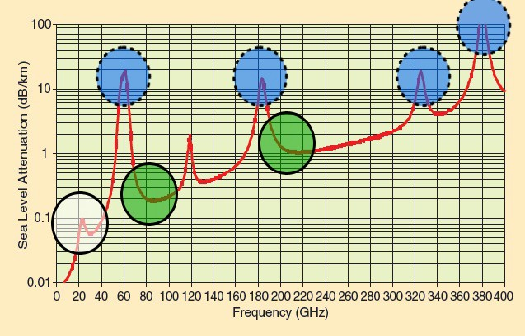
\includegraphics[width=0.7\textwidth]{Pictures/mmwave.pdf}
	\caption{毫米波频段大气衰减图\cite{rappaport2011state}}
	\label{fig:mmwave}
\end{figure}

\begin{figure}[htbp]
	\centering
	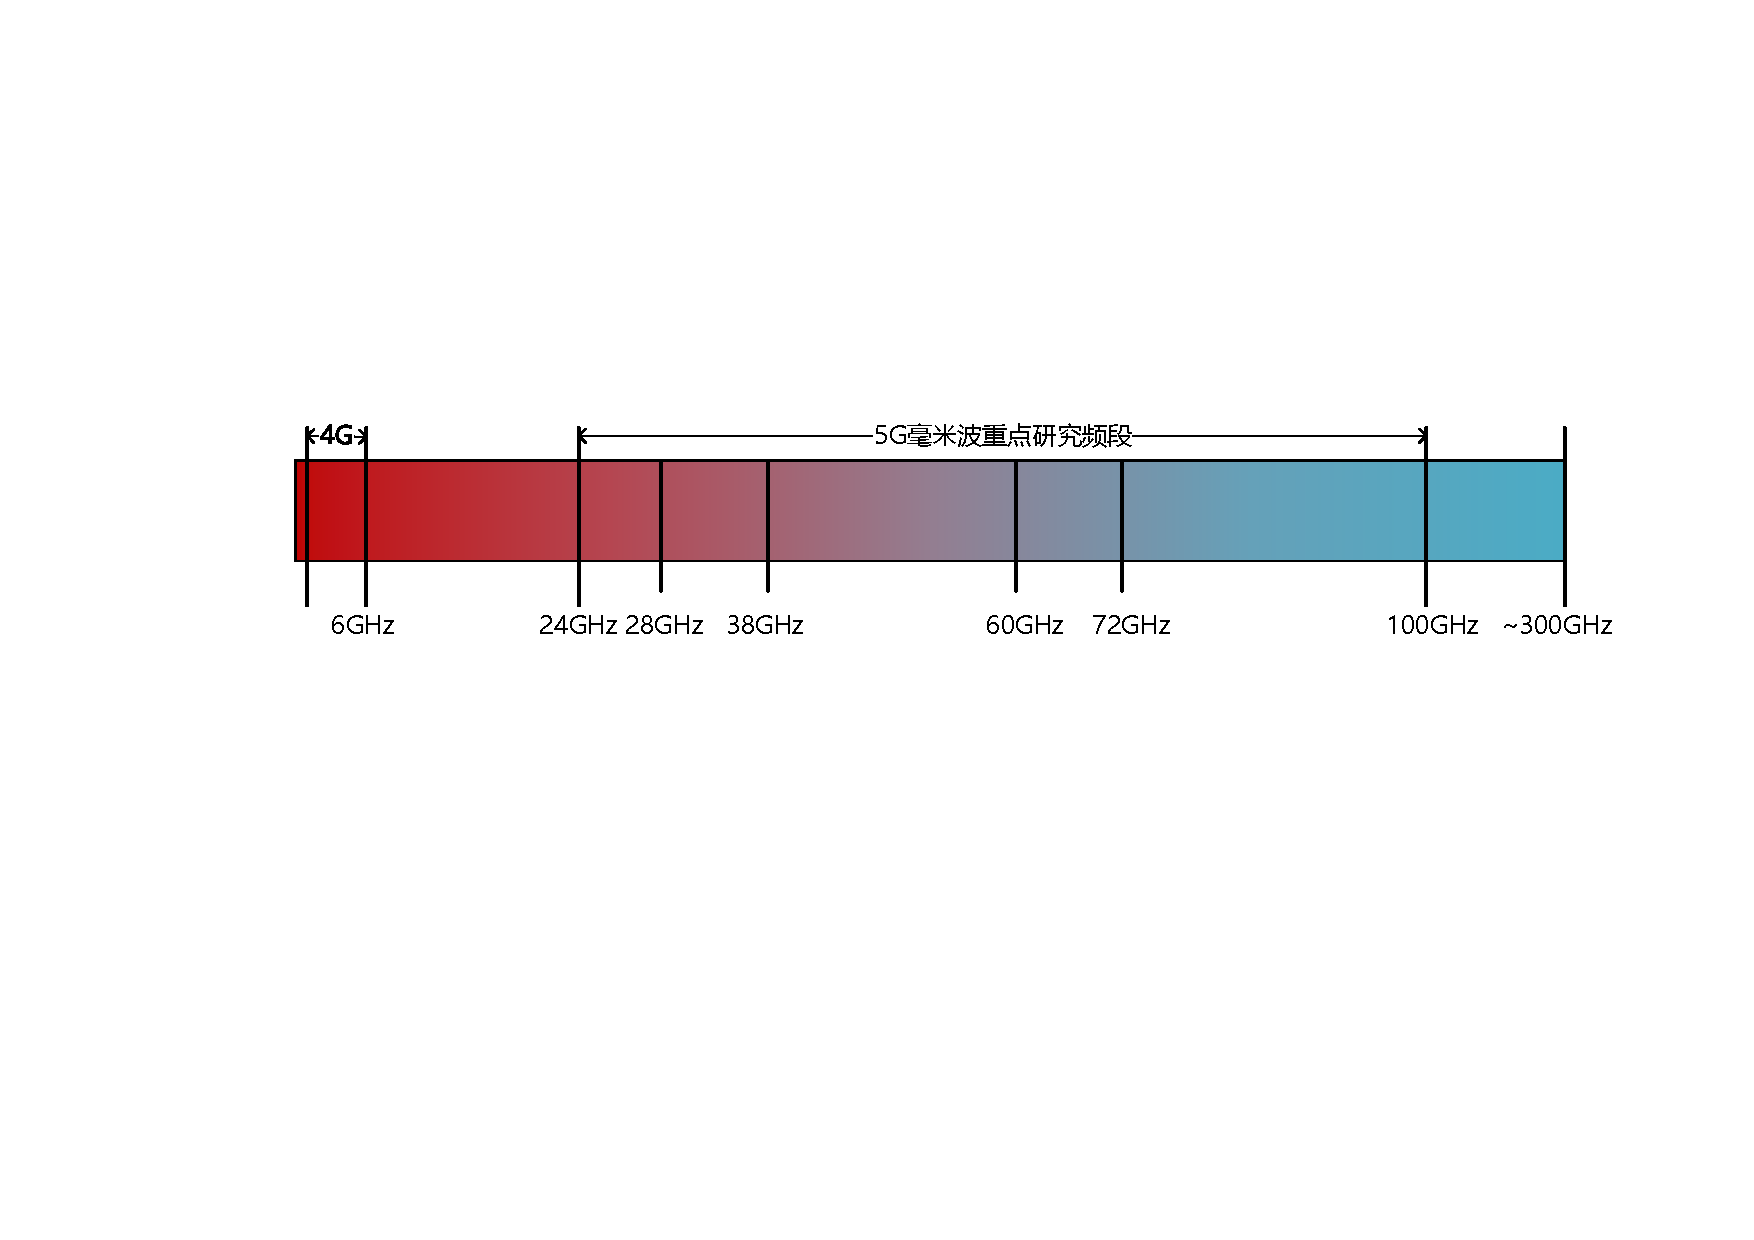
\includegraphics[width=0.7\textwidth]{Pictures/mmw.pdf}
	\caption{毫米波通信研究频谱范围}
	\label{fig:mmw}
\end{figure}

\begin{enumerate}
\item \textbf{毫米波通信技术} \quad 毫米波频段主要是指处于30-300GHz的极高频(EHF)频段,其波长在1-10毫米的范围内。该频段拥有丰富的、未被有效利用的频谱资源,能够提供高达Gbps级别的通信带宽。在传统无线通信网络中,通常是利用超高频、特高频及以下频段进行通信,而毫米波所在的极高频则通常是用于遥感卫星、射电天文学或者日常的安检扫描中,并未应用到无线数据传输领域。其原因在于虽然毫米波频段数据传输速率高,然而根据Friis自由空间衰落模型,过短的波长导致其在自由空间中的衰落速度极快,有效通信范围非常受限;同时毫米波在面对障碍物时阻挡效应严重,难以通过绕射等方式继续传播,严重影响了毫米波作为数据载体的实际应用。
近些年的研究发现,可以通过将毫米波与波束成形技术结合,将毫米波信号能量集中成方向性的窄波束进行数据传输,不但可以提高信号传输范围,还可以实现频谱资源的空分复用,提高频谱利用率;同时可以利用毫米波高速率低覆盖的特点,与致密化蜂窝小区技术结合,既可以有效地提高数据传输速率,又能避免较长的传输距离干扰其他基站小区内用户,还降低了非核心区域恶意用户的窃听机会,提高了传输数据的安全性。如图(\ref{fig:mmwave})所示为毫米波频段受大气影响的情况,在致密化小区技术的基础上,小区范围下降到200米的范围内,此时大气对毫米波的影响并不显著,尤其是在28GHz和38GHz频段\cite{rappaport2013millimeter}。现阶段毫米波通信研究主要专注在24-100GHz范围内,如28GHz\cite{pi2011introduction}、38GHz\cite{sulyman2014radio}、60GHz\cite{li2014efficient}与72GHz\cite{nie201372}等频段,见图(\ref{fig:mmw})。事实上,毫米波通信已经应用于一些无线通信标准中,如1)IEEE 802.15.3c-2009 Task Group 3c协议\cite{802153},作为第一个工作在57-64GHz频段的无线协议,首次达到了1Gbps的带宽;2)IEEE 802.11ad Wi-Fi协议\cite{80211ad},使用60GHz频段通信,最大支持32根天线,带宽可以达到4.6Gbps峰值;3)802.11ay协议\cite{80211ay,ghasempour2017ieee},作为802.11ad的继任者,是第一个真正意义上的毫米波宽带无线接入协议,它使用60GHz频段通过方向性基站进行数据传输,最高支持100Gbps的峰值传输速率,并可保证在300-500米的传输范围内得到20-40Gbps的稳定传输。

\item \textbf{波束成形技术}\quad 毫米波通信在带来更高的通信带宽同时,也带来了更快的路径衰减。为了弥补高频率带来的传输损耗,可以利用波束成形技术进行信号的发射与接收。波束成形技术建立在多天线系统的基础上,通过提高多重增益(Multiplex Gain)、分集增益(Diversity Gain)以及天线增益(Antenna Gain)以提高信号的传输效率。其中多重增益是指在多个天线上同时传输平行的多路信号,以降低误码率;分集增益是通过时空编码的方式,提高分集增益、降低误码率;天线增益是通过提高特定用户方向上的信噪比,并降低其他用户方向上的信噪比,以提高传输效率。
波束成形技术可以分为模拟波束成形技术\cite{venkateswaran2010analog}、数字波束成形技术\cite{spencer2004zero}以及混合模拟数字波束成形技术\cite{han2015large}。模拟波束成形技术通过改变每个天线单元上的信号相位,将毫米波波束能量集中到某一特定的方向上,而其他干扰方向的天线增益被显著降低,进而提高了传输的能量效率,很适合应用在室内环境的毫米波通信系统中。数字波束成形技术最早使用在传统天线数量有限的微波系统中,每个数字基带通过单独的数模(DAC)/模数(ADC)转换器控制一个天线的相位,因此相较于模拟波束成形技术能够达到更高的自由度。然而在毫米波通信中,当天线数量急速增长时,相应的硬件成本也会急剧增加,同时为每个天线单元配备一个DAC/ADC从硬件上难以实现,因此将纯数字波束成形技术用于大规模多天线阵列中并不现实。因此在未来的5G通信中,会将模拟波束成形技术与数字波束成形技术结合,利用混合波束成形技术将整个天线阵列虚拟地分成多个子阵列,每个子阵列连接在同一个射频链路上,并与一个用户进行通信。混合波束成形技术中的数字波束成形部分在基带上对信号进行预编码,当预编码过的信号通过数模转换器后,利用模拟波束成形技术将信号聚集成方向性波束与对应方向进行通信。

\item \textbf{大规模多输入多输出天线阵列技术}\quad 多输入多输出(MIMO)天线阵列系统\cite{rusek2013scaling}已经应用于现有的无线通信系统中,在4G长期演进(Long-term Evolution, LTE)标准中基站端支持最多八个天线的MIMO技术。相较于传统的单天线通信系统,在发射和接收端布置更多的天线带来了更高的自由度,更好的链接质量与更快的传输速率。MIMO技术带来了通信质量的显著改进的同时,也带来了发射接收端更高的硬件复杂度以及在信号处理中的更高的计算复杂度与能耗。5G通信系统中将MIMO系统进一步发展成为大规模(Massive)MIMO系统,在发射和接收端引入了数以百计的天线单元,以期进一步提高通信性能。在Massive MIMO系统中,天线数量将远远大于用户数量,充足的天线带来了信道硬化的特点,使得信道状态可以保持相对稳定且变化缓慢,从而使提前进行系统资源优化处理成为可能。
\end{enumerate}

\subsubsection{毫米波通信研究要点}

毫米波通信能够提供极高的通信带宽,为各种无线应用带来新的可能性,因此一直受到研究者的重视。然而毫米波信号波长过短,极易在空间中衰减,就需要利用波束成形技术将其集中成方向性波束进行传输。为了形成能量更集中、更窄的波束,需要大量的天线单元即大规模MIMO天线阵列。而大规模天线阵列的组成又是建立在毫米波信号使用的基础上:只有使用毫米波信号,天线单元的体积与单元之间的距离才能缩小到合适的范围内,进而可以将大规模天线阵列布置在发射与接收端。三者之间相互依托,密不可分。新的技术也带来了新的挑战,在这些新兴技术的支持下,如何更高效地利用系统资源提高无线通信性能,如实时性、吞吐量、能耗效率与频谱利用率等,就成为了下一代毫米波通信中重要的研究内容。本文将从三个角度进行研究,首先从毫米波方向性通信建立的基础入手,研究如何实时准确地得到多用户位置信息,以进行发射接收双方波束对准并建立连接,即毫米波通信多用户跟踪实时性问题;在此基础上,本文将研究毫米波通信在星型网络与网状网络这两类主要网络拓扑结构中的资源分配优化问题,分别将在蜂窝小区基站以及无线数据中心网络两个应用场景中进行讨论。

\begin{enumerate}
	\item 毫米波通信系统多用户跟踪实时性问题研究

	在毫米波通信系统中,极短的波长导致无线信号的衰减速度急剧增加,需要将传统的全向波转变为方向性波束以集中能量进行信号传播。毫米波只有在发射与接收波束对准的情况下才能实现其高速率的数据传输,因此毫米波通信需要需要精确的位置与跟踪信息以进行波束对准。同时由于毫米波所用天线的体积相较于厘米波段显著减小,使得将较大规模的天线布置在用户终端上成为可能。借此可以利用阵列信号处理等手段,对信号进行更准确的波达角估计,进而可以判断出与基站之间的相对方位信息,便于毫米波波束的对准与传输。同时借助空分复用等技术,基站可以在同一个频段与多个用户同时通信,这就需要同时对大量移动目标进行跟踪以便利用方向性波束通信。因此\textbf{如何提高对多个移动用户精确跟踪的实时性直接影响着用户的通信表现。}这也成为毫米波通信系统中重要的研究课题之一。在毫米波无线通信中,系统对实时性要求有了进一步的提高:感知网络(Tactile Internet)中所提出的实时性要求网络反应时间小于对应应用的某些时间常量,例如人体感知延迟的水平,即1毫秒\cite{fettweis20145g}内。因此提高对通信范围内多个目标的跟踪精度与实时性就尤为重要。本文将在毫米波通信系统中针对多个可移动用户的跟踪实时性问题进行研究。

	\item 星型网络结构毫米波通信系统资源分配与优化问题研究

	作为星型网络结构(Star Network)的典型应用之一,蜂窝移动通信系统是毫米波通信的一个主要应用场景。蜂窝系统中的基站资源管理与优化问题一直是重要的研究问题,且在引入毫米波通信等新兴技术后又出现了诸多新的挑战,如干扰对齐、绿色通信、天线分配等。系统需要对包括计算资源(运算核心)、通信资源(天线数量)、能量资源(传输功率)、频谱资源(信道分配)等在内的资源进行合理分配,以最大化系统效益。在基站-用户场景中,用户只拥有较少数量的资源而基站则拥有大量可利用资源用以分配。\textbf{如何分配基站的天线资源以提高整个系统的吞吐量}就成为了一个重要的研究问题。对此本文将在单小区单基站多用户的场景下进行研究,考虑基站端天线资源的优化问题以提高5G毫米波通信系统吞吐量等性能。

	\item 网状网络结构毫米波通信系统资源分配与优化问题研究

	此外,作为网状网络结构(Mesh Network)的典型应用之一,数据中心网络也是毫米波通信的另一个主要应用场景。该场景下通信双方都拥有较强的通信与计算能力,能够在授权或者非授权频段建立彼此之间的直接通信而无需通过基站进行数据传输\cite{asadi2014survey}。此时收发双方之间所拥有的通信资源规模相当,数据传输表现与双方都直接相关。与之前星型网络场景不同的是,在本场景中发射和接收双方可以进行同等水平的资源分配与优化。因此,\textbf{如何建立无线数据中心网络并在给定任务负荷下优化调整系统内发射接收对的通信资源以提高整个系统的通信效率}就成为一个重要的研究问题。本文将在无线数据中心网络场景下进行资源优化分配研究以提高数据中心网络的性能表现。
\end{enumerate}

\section{研究现状}

\subsection{毫米波通信系统多目标快速跟踪}

相较于传统无线通信系统,毫米波通信系统对用户定位精度和实时性要求更高。这主要体现在毫米波通信使用的是较窄的波束进行方向性通信,只有在准确的知道用户位置信息时才能进行波束对准。且用户经常处于运动中,需要在对其进行定位的同时进行波束跟踪,以提供持续性的高性能服务。由于毫米波天线阵列的特点,在只存在视距传播路径的情况下,可以进行更精确的波达角(Direction of Arrival, DoA)估计,再加以准确的到达时间(Time of Arrival, ToA)即可得到精确的用户位置信息。
Maccartney等人研究了73GHz频段毫米波信号在野外大基站小区内的传播模型\cite{maccartney2017rural,maccartney2017study},在3GPP/ITU-R的室外大基站CI模型的基础上,加入基站高度对信号传播的影响,提出了更加准确并已实施的CIH衰落模型以利于更准确的距离定位。
Savic等人提出了利用分布式Massive MIMO系统进行基于指纹的定位方法\cite{savic2015fingerprinting},在高杂波多径反射的环境中,采集用户的接收信号强度(Received Signal Strength, RSS),在只存在一个基站的情况下,利用贝叶斯非参高斯过程回归方法对用户进行高精度定位。
Koivisto等人提出了在超致密小区结构中联合设备定位与时钟同步的方法\cite{koivisto2017joint,koivisto2017high},利用基于扩展卡尔曼滤波(Extended Kalman Filter, EKF)的算法对ToA和DoA进行估计,并通过二阶段EKF对ToA和DoA进行融合估计用户位置,其提出的级联式EKF算法即使在实际工作场景下,依然能够得到移动用户米级别的定位精度以及微秒级别的时钟同步。
Cui等人提出了利用毫米波信号对车辆进行定位的方法\cite{cui2016vehicle},通过设计合适的脉冲信号波形,利用两种接收机测量时间并得到精确的位置信息,其中能量检测器消耗较低的计算复杂度,得到较高的时间测量精度;而相干接收器通过消耗更高的计算复杂度,能够得到更高的时间测量精度。

在移动通信场景中,用户通常会在一定范围内运动,因此需要在准确定位的基础上对这些移动用户进行波束跟踪,以保证基站与用户之间的连续高速率通信。通常做法在得到用户的测量位置(角度)信息后,利用各种滤波算法对收到的信息进行滤波以重新估计用户的精确位置(角度)。
日本NTT DOCOMO公司研究了在室内多反射场景下利用70GHz频段毫米波与移动性目标进行通信的问题\cite{inoue2015experimental},当用户按照$2$km/s的速度运动时,无论是在有反射或是无反射墙壁的情况,或是障碍物存在与否,系统都可以得到高达2Gbps的通信速率。
之后三星公司与DOCOMO共同研究了在户外场景下利用28GHz频段毫米波超宽带无线信号与高移动性用户进行通信的问题\cite{obara2016experiment},在基站使用48个天线单元组成的平面天线阵列,通过混合数字模拟波束成形技术将毫米波信号将极窄的波束发射到拥有4个天线组成的均匀线性阵列的移动设备上。实验证明了即使用户在处于$60$km/s的运动速率时也能够得到约4Gbps的高通信速率。
Tateishi等人研究了在室内场景下利用15GHz频段对移动目标进行波束跟踪的问题\cite{tateishi2016indoor},证明了即使存在丰富的多径路径情况下,用户仍然能够在50米的距离达到7.7Gbps的峰值下行速率。
Kim等人研究了在OFDM毫米波无线通信系统中的波束跟踪问题\cite{kim2018beam},在多小区多用户的场景中,设计将基站天线阵列分成两个子阵列,通过特殊的导频设计可以区分不同的子阵列的信号,并计算两者的相位差得到波束发射角(Angle of Departure, AoD)与波束到达角(Angle of Arrival, AoA)并以此进行多用户跟踪。
Suhanya等人提出了一种鲁棒性的波束跟踪算法\cite{jayaprakasam2017robust}。在固定的基站运行扩展卡尔曼滤波,并通过EKF估计出的误差协方差来鲁棒地更新波束成形权重。
Vutha等人研究了在模拟波束成形场景中通过只训练一个波束对来跟踪一条轨迹的方法\cite{va2016beam},此设计同样也利用了扩展卡尔曼滤波作为跟踪滤波算法,并证明了在同样的信噪比情况下,较窄的波束对角度改变更加灵敏,因此能够提供更高的跟踪精度,然而过窄的波束也同时容易导致波束错位,降低跟踪的精度。
Yu等人则研究了在慢衰落MIMO干扰信道中波束跟踪对于干扰校准的影响\cite{yu2012beam},通过应用矩阵扰动理论混合特征分解和预测过程以最小化干扰校准预测步骤的复杂度,该算法能够使用更低的计算复杂度得到与传统算法相似的跟踪效果。
Wei等人提出了利用毫米波无线射频进行高精度无源用户跟踪的方法\cite{wei2015mtrack},并将跟踪精度提高到了分米的级别,通过高方向性的60GHz毫米波波束扫描发现用户的初始位置,并降低环境中背景反射造成的干扰,最后利用基于信号相位的模型对用户路径进行跟踪。

在毫米波通信系统中,大部分研究工作关注单目标的定位与跟踪问题,很少涉及到多目标跟踪领域;且多着重于跟踪精度提升,对跟踪实时性研究较少。本文着眼于毫米波通信中的多目标跟踪实时性问题,为毫米波通信建立位置信息基础。

\subsection{毫米波蜂窝系统基站资源分配与优化}

蜂窝小区网络是毫米波通信的重要应用场景之一,其主要由基站及众多用户组成,是一种典型的星型网络拓扑结构。现有蜂窝网络技术中引入了MIMO技术,利用多个天线组成的天线阵列,通过空时编码与波束成形等技术实现了空间分集和空间复用,提高了信道频谱利用率。
在引入毫米波通信后,为了进一步提高天线系统的增益,美国贝尔实验室的科学家 Marzetta 在MIMO技术的基础上,于2010年最早提出了适用于毫米波通信的Massive MIMO天线系统概念\cite{marzetta2010noncooperative}。假设在一个时分双工无线通信系统中,基站拥有无限数量的天线资源,即可在同一个时间频率上与多个用户分别通信。之后Rusek等人认为在目前的理论研究及硬件实现中,可以定义大规模MIMO系统中的基站天线数量在100到1000个天线终端范围内\cite{rusek2013scaling},同时该系统符合随机矩阵理论中的一些渐进结果,例如信道中的奇异值分布会趋向于具有确定性的函数等。不仅如此,使用大规模MIMO阵列天线还可以大幅度提高频谱与能量利用效率\cite{lu2014overview}。由于系统采用TDD的方式,上下行信号在同一个频段内通信,在很短的时间内可以认为上下行信道是具有相互性(Reciprocal)\cite{bjornson2016massive}的,即两个方向上的信道响应是相同的。可以通过上行信号的信道响应得到信道状态信息(Channel State Information, CSI),并对上下行信道进行估计,因此可以通过增加基站天线数量来提高系统性能\cite{marzetta2006much}。在多基站多小区的情况下,由于正交信道导频数量远小于用户数量\cite{marzetta1999blast},相邻基站用户非正交导频会带来导频污染问题。但是当基站天线数量无限增长时,会出现信道硬化(Channel Hardening)\cite{hochwald2002space,hochwald2004multiple}的特性,非相关噪声与快速衰落效应都将消失,只剩下由于导频污染导致的小区间干扰影响系统表现,随机的无线信道特性趋向于确定\cite{wangxinshui}。在此基础上,Hoydis等人\cite{hoydis2013massive}研究了当Massive MIMO系统中基站天线数量相较于用户数量并非无穷大时的系统表现,并给出了计算每个用户需要多少数量的天线以满足一定比例的无限天线系统极限表现的方法。同时证明了通过最小均方误差法(MMSE)和正则迫零法(RZF)可以在节省较多天线资源的同时达到特征值波束成形法与匹配滤波所能得到的效果。在这类场景中可分配资源通常包括天线资源、用户配对、信道分配或是能量分配等。而其优化目标一般为最大化系统吞吐量、频谱利用效率、能量利用效率或是最小化通信误差等目标。

在频谱资源优化方面,4G中主要使用正交频分复用(Orthogonal Frequency Division Multiple Access, OFDMA)技术\cite{holma2009lte}。在5G的研究中,除计划继续使用TDMA、FDMA或OFDMA等正交方法之外,有研究认为可以采用如半正交多址接入SOMA\cite{khormuji2015generalized}、稀疏编码多址接入SCMA\cite{nikopour2013sparse}、交织多址接入IMDA\cite{ping2006interleave}等非正交多址接入(Non-orthogonal multiple access, NOMA)类技术\cite{saito2013non,dai2015non},将多个用户的信号在能量域上叠加,在接收端利用连续干扰消除的方法逐步提取目标信号,此时所有用户可以在相同的时间使用相同的频率与编码进行通信,这将极大提高系统频谱利用率。

在能量利用效率方面,毫米波通信系统中的绿色通信被列为重点研发方向。事实上电力资源消耗是通信运营公司的主要运行成本,因此提高毫米波无线传输能量利用效率具有重要的研究意义。
Bj{\"o}rnson等人研究了如何在Massive MIMO系统中得到最优的能量利用效率\cite{bjornson2015optimal},提出了最优能量效率与天线数量、活动用户数量以及发射功率之间的闭式关系。
Ngo等人证明通过使用Massive MIMO系统可以提高频谱利用率的同时更好的提高能量利用率\cite{ngo2013energy},只需通过MRC,ZF等简单的线性过程,通过对上行导引向量进行信道估计即可降低小区内的干扰,同时权衡了频谱利用率与能量利用率以得到最优的系统收益。
Shi等人则研究了多小区Massive MIMO系统的小区上行覆盖范围优化问题\cite{jin2015cell}。通过应用在基站上的倾斜可调整的天线阵列可以优化小区覆盖范围,中和小区边缘覆盖与导引向量污染的问题。同时文章对不同小区形状以及用户性质的情况进行了分析,通过简单的线性查找即可得到最优覆盖方式。
为了得到准确的信道状态信息,大部分工作都将研究注重于时分双工系统,即上下行信道只有时域上的区分,在频域上保持有相互性。然而Adhikary等人研究了在移动通信中普遍使用的频分双工(Frequency Division Duplexing,FDD)系统\cite{adhikary2013joint}中的CSI问题。由于不能利用上下行信道的相互性,系统需要利用联合空间分集与复用技术(JSDM)在FDD通信系统中获取即时信道状态信息,并借此方法只需通过较少的二阶统计信息即可得到有效地空间分集增益。

现有研究工作中大部分都针对传输信道、能量以及波束成形权重等要素进行资源优化,很少有针对大规模天线阵列本身天线单元的资源优化研究。随着阵列天线上天线数量的增多,天线单元本身也成为需要优化分配的重要资源。本文将针对蜂窝小区基站天线阵列中天线资源本身及其子阵列形状适配等优化问题进行研究。

\subsection{毫米波无线数据中心网络资源分配与优化}

数据中心网络(Data Center Network,DCN)是毫米波通信的另一个重要应用场景,也是一种典型的网状网络拓扑结构。随着大数据、云计算、人工智能、超级计算等新技术在各个领域的运用越来越广泛,数据中心对海量数据的储存与传输变得越来越重要。其中数据中心网络通过电缆、光纤和无线等方式建立高效的拓扑结构,将多种物理单元连接起来,负责着极为重要的通信功能。

早期的数据中心网络流量主要以南北向流量(North-South Bandwidth)为主,即数据中心外到数据中心服务器之间进出的流量。然而随着大数据等科技的应用,东西向流量(East-West Bandwidth)即数据中心服务器之间的流量越来越重要。 按照Cisco公司发布的全球云指数白皮书\cite{cisco2018cloud}预测,到2021年$85\%$的数据中心流量将会是服务器之间或数据中心之间的东西向流量,而服务器与外界互访的南北向流量将会下降到$15\%$左右。许多很小的应用将会需要动态调动大量的数据传输,传统的多层数据中心网络将难以满足强大的传输带宽需求。因此有研究者考虑使用灵活性更高的无线方式动态地进行服务器/机架间的点对点通信,以降低通信热点的发生,降低系统传输时延。

有线数据中心网络主要分为两大类,一类是简单的树状结构,在接入层使用接口较少的廉价交换机,汇聚层使用接口较多也更昂贵的交换机,而在核心层使用拥有数百个万兆接口的极为昂贵的高性能交换机以满足数据分发的需要。这种结构对核心层网络设备有极高的性能要求,而且当服务器数量和拓扑结构发生改变时,难以满足可扩展性的需求,同时容易带来带宽超额(oversubscription)的问题。

\begin{figure}[t]
	\centering
	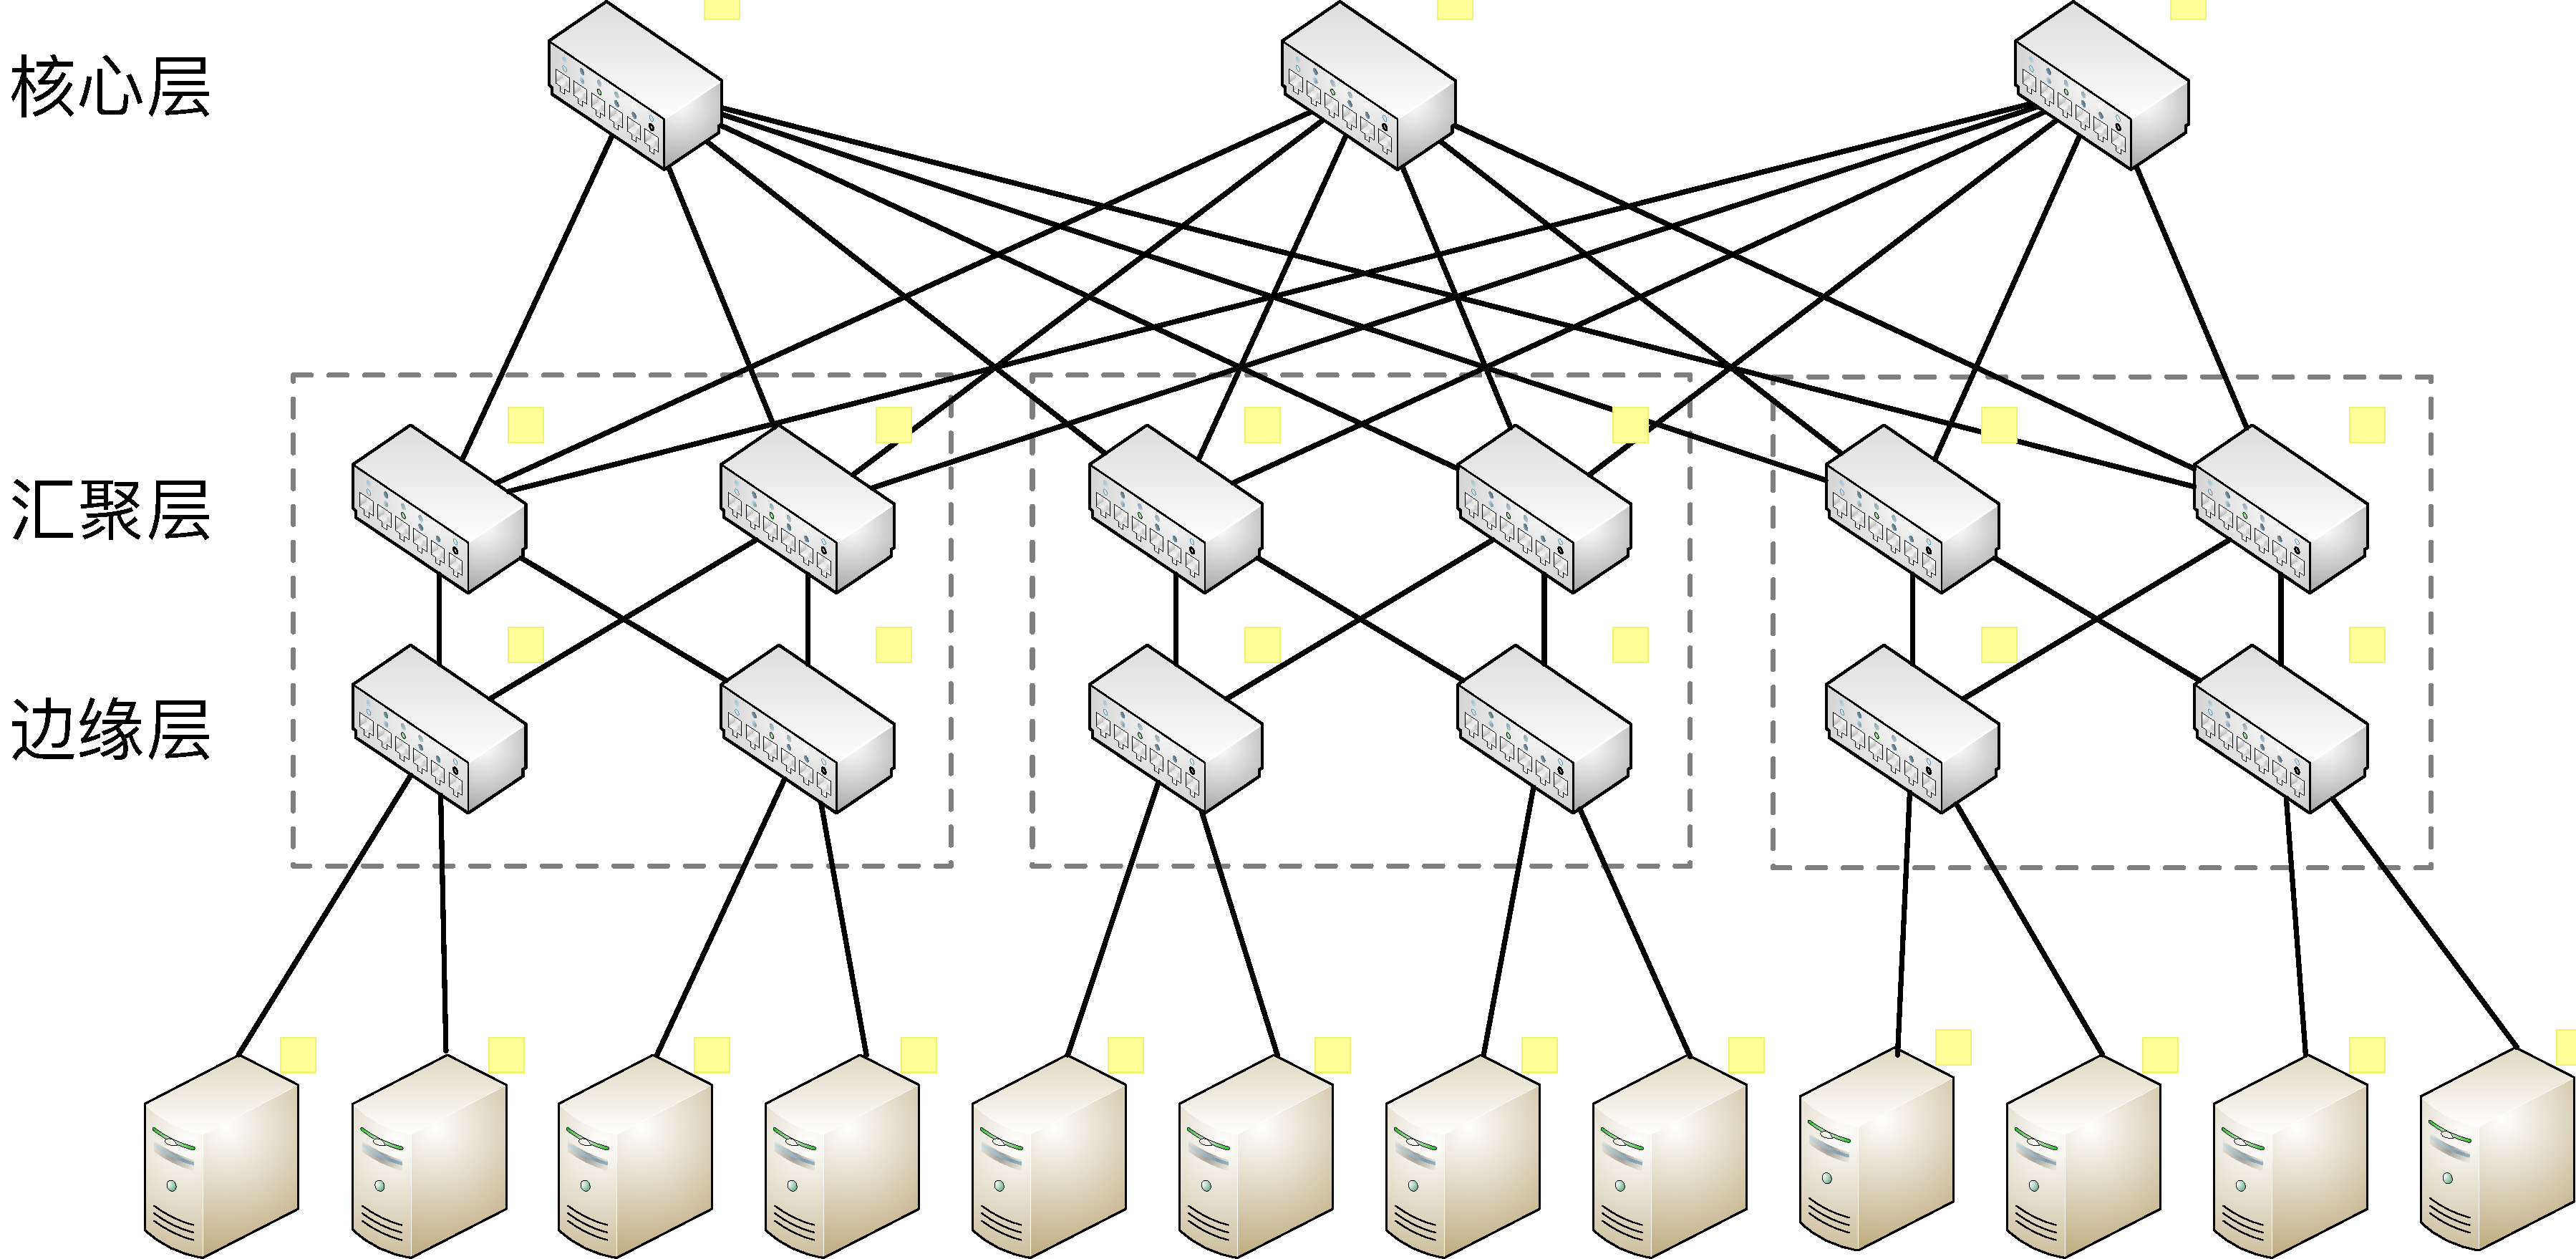
\includegraphics[width=0.7\textwidth]{Pictures/fattree.pdf}
	\caption{Fat-tree数据中心架构示意图}
	\label{fig:ft}
\end{figure}

\begin{figure}[t]
	\centering
	\includegraphics[width=0.7\textwidth]{Pictures/helios.pdf}
	\caption{Helios数据中心架构示意图}
	\label{fig:helios}
\end{figure}


现有的数据中心网络主要为分级的互联网络结构,利用交换机将各个物理结构进行连接\cite{xia2017survey,chen2016features}。通常是一种分级的胖树(Fat-tree)型互联模型网络架构,通过加入冗余的带宽和交换机阵列,使用经济的平价交换机代替昂贵的高性能交换机,同时冗余交换机的引入也缓解了单点失效的问题。

传统的有线数据中心网络一般主要包含三层:核心层(Core Layer)、汇聚层(Aggregation Layer)和接入层(Access Layer)。
\begin{enumerate}
	\item 核心层负责数据中心流入流出的路由功能,提供与大量汇聚节点的丰富连接。
	\item 汇聚层提供核心层与接入层之间的连接,同时也提供防火墙、负载平衡、流量汇聚与应用加速等服务。
	\item 接入层连接服务器与数据中心网络,是整个架构中最底层的结构。
\end{enumerate}

多余的冗余交换机在带来对等带宽的同时也带来了巨大的资源消耗,如图(\ref{fig:ft})所示。主要包括三种类型,以交换机为核心的架构(Switch-centric topologies),以服务器为核心的架构(Server-centric topologies),以及各种增强型架构。
在以交换机为核心的架构中 \cite{singla2012jellyfish,walraed2013aspen},交换机处于多层级架构中的高层位置,而服务器处于网络边缘较低层的位置。
Fat-tree拓扑结构 \cite{al2008scalable}是在传统树形结构的基础上改进的三层拓扑结构。在Fat-tree架构中,系统主要由自上而下的核心层、汇聚层和边缘层构成,边缘层与服务器相连。各层级的交换机为同型号交换机,且每个节点的上下行带宽保持相等。同时对于任意两个服务器之间都有着多条相同代价的传输路径,因此理论上可以得到完全对等的带宽。然而这种架构使得交换机之间的接线非常复杂且冗余。
VL2 \cite{greenberg2009vl2}是与Fat-tree类似的三层树状拓扑结构。只是每个边缘层交换机都与两个汇聚层交换机相连,而汇聚层与核心层之间的交换机则以完全二部图的形式相连接。在提高了交换机之间线缆带宽的同时减少了总体线缆数量。

在以服务器为核心的模块化数据中心架构中,服务器吸纳了更多的连接与路由功能,除了作为拓扑网络中的终端节点外,更成为彼此间的中继节点。作为组网与路由的核心,服务器的作用变得更加重要,交换机则只作为单纯的数据转发。微软亚洲研院在2008到2013年间陆续提出了DCell\cite{guo2008dcell}、FiConn\cite{li2009ficonn}、BCube\cite{guo2009bcube}、MDCube\cite{wu2009mdcube}以及CamCubeOS\cite{costa2013camcubeos}等数据中心网络拓扑架构。
其中DCell\cite{guo2008dcell}是一个典型的以服务器为核心的递归型数据中心拓扑架构。在最底层的0-层,有n个服务器直接与一个交换机相连;这样的n+1个0-层结构构成了1-层DCell架构,每个0-层结构中的服务器提供一个端口与另一个0-层结构中的服务器相连,若将0-层结构看做是一个虚拟节点,则整个1-层形成一个完全图网络。因此DCell结构提供了很强的可扩展性。然而此架构中网卡数量指数级增长,且系统仍为有阻塞的架构。
FiConn\cite{li2009ficonn}则考虑到实际系统中,服务器与交换机的物理网卡接口数量的限制,将服务器端的物理网卡接口数量设置为2个,在此基础上以多层递归的形式将网络连接起来,这可以被认为是低连接度版本的DCell架构。与DCell类似,FiConn也是由相同的基本单元构成的递归型架构,相较于DCell减少了大量的网络传输线路,也降低了布线的难度。
BCube\cite{guo2009bcube}可以看作是集装箱式的模块化数据中心结构。它与DCell架构类似,也是一个递归型的以服务器为中心的拓扑架构。在0-层架构中与DCell相同,也是有n个服务器直接与一个n接口交换机相连;在上层的k-层结构中,都由n个k-层结构组成,每个交换机与每个(k-1)-层中的服务器相连。可以认为BCube是Fat-tree与DCell权衡后的结果:相较于Fat-tree结构而言,BCube节省了交换机的数量,但是增加了网卡数量,并能够提供更好的一对多服务;而相较于DCell而言,BCube提高了网络转发效率,能够提供更高的网络容量。
MDCube\cite{wu2009mdcube}则是将多个BCube连接起来,已适用于超大规模数据中心网络。其引入带宽更宽的光交换机用于BCube集装箱式模块之间的通信,而BCube集装箱式模块之内的通信仍使用传统电交换机。

随着数据量的极速增长以及服务器间数据流量的增加,数据中心对传输带宽的要求逐渐升高,传统的电缆连接已渐渐不能满足高速数据中心网络的需求;同时随着商业光通信交换机设备的价格逐渐降低,基于光信号传输的系统架构映入研究者的视线。光交换机可以有选择地将光纤中的光信号进行转发,能够提供巨大的传输带宽。现有工作主要是将光信号交换机与现有电信号交换机混合组网,以提高传输速率。一般而言,电信号交换机通常仍组成树状结构,而光交换机则采用单跳的方式连接两个服务器。

早在2005年Barker等人就提出利用光路交换机\cite{barker2005feasibility}降低数据中心网络的通信成本。在高性能计算机系统中建立两套通信网络,一套利用光路交换机(OSC)价格便宜且能耗较少地满足长期且大量的数据交换,另一套则使用电包交换机(EPS)用来满足短期的低带宽数据交换。光路交换机系统使用了较少的光学传输设备,能够显著的降低数据中心网络成本。
Wang等人引入了基于MEMS的光学交换机\cite{wang2009your},组成混合包交换/电路交换网络。设计可以提供更易用的全数据包网络,同时低成本地为一些高级的应用提供了更高的带宽。
Helios\cite{farrington2010helios}提出了混合电子/光学交换机架构,可以大量减少交换机数量、线缆和能源消耗等,这是一个2层的多根树状结构,利用被动光学分路器(Mux)承载不同波长的信号进行高容量的单跳通信,并通过最大最小公平进行带宽的估计,如图(\ref{fig:helios})所示。
2011年Wang等人提出c-Through\cite{wang2011c}在原有有线数据中心网络的架构中,引入了高带宽低复杂度的MEMS机架间光路交换机。通过波分复用技术(Wave Division Multiplexing, WDM)显著提高了总通信带宽。提高了数据中心网络的通信带宽。
Helios与c-Through的区别在于Helios在交换机上进行流量估计与流量多路分解,而c-Through则在服务器端进行流量控制。 c-Through的优势在于可以通过服务器进行数据缓冲,并打包将数据进行转发,使得光学路径传输更加高效。
Helios在交换机上实现流量估计与多路分解的工作,虽然使得整个流量控制对终端透明,但是需要更新所有的交换机设备。而c-Through则将数据缓冲在终端设备上。两者体现了在混合有线数据中心网络设计上不同的权衡方式。
OSA\cite{chen2014osa}在c-Through和Helios的基础上建立光路单跳网络,依靠Hedera\cite{al2010hedera}在理想无阻碍网络中进行基于最大最小平等带宽分配方式分配TCP流量。进而通过多个单跳连接缝合技术建立所有服务器间的通信网络。此外还可以动态调整光路链接的带宽,以更细粒度地适应数据传输需求。
Sun等人提出了基于Fat-tree模型的改进的Diamond\cite{sun2014diamond}结构。它用边缘交换机替换掉Fat-tree模型中所有汇聚层的交换机,并将边缘交换机与核心交换机直接连接。相较于Fat-tree模型,通过此方法可以有效的降低端到端(End-to-End)的时延。
最新的一些研究已经开始使用毫米波无线通信加强数据中心网络,其中包括使用喇叭状天线\cite{halperin2011augmenting},或是阵列天线3D波束成形\cite{zhang20113d,zhou2012mirror}等技术建立点对点无线链接。

现有研究工作主要通过建立新型拓扑结构等方式对数据中心网络进行优化。在引入毫米波通信后服务器间的通信变得更加多样化与自由化,预期可以极大的提升网络性能。利用毫米波高速通信建立无线数据中心网络架构的研究方兴未艾,本文中也提出一种基于阵列天线的点对点视距通信毫米波无线数据中心网络设计,并对其阵列天线资源进行优化分配研究。与星型网络不同,这种网状网络中任意两者之间都有可能发生通信,通信的双方所拥有的资源处于着相同的水平且不需要通过基站建立通信。此时只针对基站等资源优势的一方进行资源分配与优化难以得到系统的最优解,需要同时对发射与接收双方进行资源的分配与优化。

\section{本文研究内容}

\subsection{研究思路}

本文研究在下一代毫米波无线通信系统中的资源分配与优化问题。全文的思路和基本组织结构如图(\ref{fig:the})所示。第一章介绍了下一代毫米波无线通信系统,及其相关的多目标跟踪实时性与资源优化分配问题的研究背景及研究现状;第二至四章为本文的主体部分,其中第二章研究了毫米波无线通信系统中多目标跟踪实时性问题,提高了用户位置信息获取的实时性,为后续第三、四章不同网络拓扑场景下的毫米波通信建立了基础;之后第三章研究了星型网络拓扑下的毫米波通信资源分配问题,主要针对蜂窝小区中基站侧天线资源进行优化;接着在第四章研究了网状网络拓扑下的毫米波通信资源优化分配问题,主要针对无线数据中心网络中机架天线资源进行优化;第五章对全文做了总结与展望。

\begin{figure}[t]
\centering
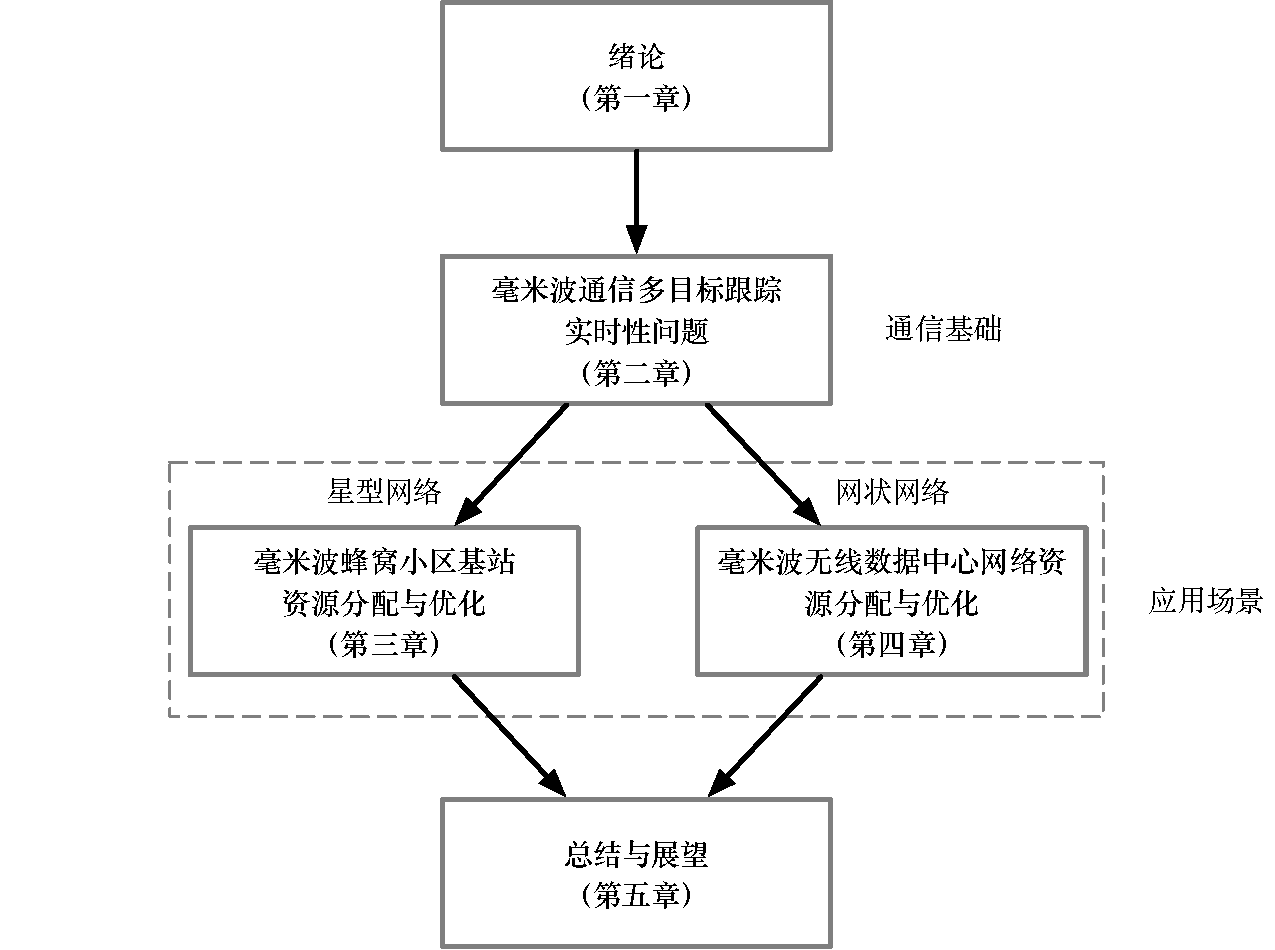
\includegraphics[width=0.9\textwidth]{Pictures/zongjiegou.pdf}
\caption{全文组织结构}
\label{fig:the}
\end{figure}

\subsection{研究内容}

本文的具体研究内容如下:

第二章研究了毫米波通信系统中的多用户快速跟踪问题。由于毫米波通信与波束成形技术的引入,基站会通过很窄的波束与用户进行通信。精确的用户位置信息能够帮助更好地进行波束对准,因此基站需要准确地感知并估计小区内处于移动中的用户的个数及其各自位置信息,这就是一个多目标跟踪问题。同时,准确而快速的跟踪意味着更低的通信时延,因此毫米波通信中多目标跟踪的实时性也亟需提高。现有的高效多目标跟踪算法,如概率假设密度粒子滤波算法等,由于其中重采样算法的限制,难以做到流水线化计算,制约了实时性的进一步提高。本章提出一种改进的重采样算法,通过引入粒子复制序列集合以及待复制粒子序列,使得需要重采样的粒子在只获得自身信息与之前重采样粒子信息的时即可进行粒子复制运算,而不用等待所有粒子完成权重值过滤后才能继续重采样。通过引入此改进的重采样算法,整个概率假设密度粒子滤波算法能够实现完全流水线化的运算。在此基础上,本文提出基于多核处理器硬件平台的计算资源分配优化算法,通过解决一组混合整数规划问题,得到了高时效的近似解法。仿真结果验证了提出的算法在保证跟踪精度的情况下,能显著降低整个滤波算法的计算时延,有效地提高了用户跟踪的实时性,为基站中每个用户的低时延通信提供了保证。

第三章研究了毫米波通信在星型网络拓扑下的典型应用——蜂窝小区网络中的资源优化问题。基站在已知小区内多个用户位置的情况下,优化分配资源以最大化系统收益即吞吐量。基站上的大规模天线阵列虚拟的分成若干个均匀线性子阵列,分别通过波束成形技术与对应的用户进行通信。由于大规模天线阵列与每个均匀线性子阵列都有着一定的固定的形状,因此问题建模为如何在矩形阵列中合理的放置这些子阵列,使得系统收益最大,这既需要考虑每个用户所占用子阵列的天线的数量,又需要考虑这些子阵列在矩形阵列中的位置分配。此场景根据不同的子阵列放置方式,又包含了两种不同的情况:1)所有线性子阵列都互相平行且平行于矩形阵列的一条边;2)为了进一步提高系统收益,线性子阵列可以平行于矩形阵列的任意一条边,即存在相互垂直的子阵列。对两种情况分别进行问题建模,对两个NP难问题进行分解并逐步求解。通过解决一系列的多选择背包问题,多背包问题和带状装箱问题,得到了两种情况下多项式时间的近似算法,并给出了每个算法的计算复杂度和下界。仿真结果验证了提出的两种算法在不同的情况下都能有效地分配天线资源,得到有性能保证的系统收益。

第四章研究在毫米波通信在网状网络拓扑下的典型应用——无线数据中心网络中的资源优化问题。在下一代数据中心网络中利用毫米波高速无线传输代替传统服务器间有线连接,以提高数据中心网络灵活性及可扩展性等。随着数据流量特性的变化,网络中出现了流量极度不平衡现象,降低了整个网络的通信性能。数据中心的机房环境相对稳定,服务器间位置也相对密集且固定,因此可以通过60GHz毫米波无线通信建立服务器间点对点直接连接,减小通信热点带来的通信性能下降。设计在每个服务器机架顶(Top of Rack, ToR)布置毫米波天线,并提出适用于阵列天线的点对点视距通信六边形机架布置方案,同时建立了单层和三层的数据中心无线网络拓扑结构,提出了对应的网络节点与边生成方式。进而对建立的无线数据中心网络结构提出了天线资源优化分配问题,通过变量替换等方式将其转化为一几何规划问题进行求解。仿真结果验证了所提出毫米波无线数据中心网络结构与优化算法能够有效降低系统的最大通信时延。

\chapter{绪论}

\textbf{本章摘要:} 本章首先介绍了移动网络发展概况及移动网络效用优化的重要意义、网络外部性效应的基本概念及其在移动网络中的体现,阐述了对于本文研究主题以及研究视角的思考; 
接着分析总结了近些年国内外涉及到与本文中三个移动网络效用优化问题相关的研究现状;
最后概述了本文的研究思路和研究内容及论文结构。

\textbf{关键词:} 移动网络;效用优化;网络外部性;研究背景;研究现状;研究内容

%\keywords{毫米波通信;5G;资源优化}

\section{研究背景}
%当今世界是一个网络的世界,各种形式的网络在人们生活中随处可见、无处不在。例如,由移动设备作为节点,由通信链路连接而成的移动通信网;社交网络是由每个人作为节点,每条边由人们之间的社交关系定义;电力网络则是由包含了发电站、配电站、工厂、办公楼、电动车充电站等电力设施以及它们之间的电力传输线路所组成的网络;而交通运输网络则是由各个运输枢纽以及连接他们的运输线路、运输工具所定义的。这些客观存在的以及人们创造出来的网络充斥着整个社会和我们的生活。

%当今的世界是一个网络的世界,各种形式的网络在人们生活中随处可见、无处不在。
%\subsection{移动网络性能优化}

21世纪见证了人类进入到以网络为核心的信息时代。现实社会中的群体与设施越来越多地呈现出网络化的特征,使得当今世界俨然发展成为一个网络的世界。不论是实体网络(如通信、电力、交通等基础设施网络),还是虚拟网络(如使用同一产品的用户网络、彼此间存在社交联系的社交网络),各种网络自身的结构特征与网络节点之间的信息交互都深刻地影响着网络整体以及网络中每一个参与个体的效用(Utility)。随着通信网络技术迅猛发展和移动智能终端广泛普及,移动网络以其突出特点和优势,越来越成为人们学习、工作、生活离不开的新空间和经济社会发展最具生机活力的新领域。与此同时,人们对移动网络的服务质量的要求日益增高、对隐私保护和安全风险的担忧日益加深,对网络资源分配的高效性与公正性更加关注,迫切要求从更广泛和多维的视角对移动网络理论、技术及机制进行创新性研究,以引领和推动移动网络更好地造福人类。


%在通讯技术的高速发展下,现代人类社会中的群体与设施越来越多地呈现出网络化的特征,使得当今的世界俨然发展成为一个网络的世界。不论是实体网络(如通信、电力、交通等基础设施网络),还是虚拟网络(如使用同一产品的用户网络、彼此间存在社交联系的社交网络),网络自身的结构特征与网络节点之间的信息交互都深刻地影响着网络整体以及网络中每一个参与个体的效能(Utility)。
%这其中包括,由移动通信设备作为节点、通信链路连接而成的移动通信网,节点对应每个人、连边代表人与人之间社交联系的社交网络,由发电站、配电站、工厂、办公楼、电动车充电站这些电力设施以及它们之间的电力传输线路所组成的电力网络,以及由各个运输枢纽与连接他们的运输线路、运输工具所定义的交通运输网络。

\subsection{移动网络的发展}

本文所研究的移动网络(Mobile network),泛指用户使用移动智能终端设备(如智能手机)依托各种无线通信技术,进行文本、语音、图像等多种类型的数据传输,使用包括移动社交、媒体资讯、在线游戏、电子商务、移动物联网在内的多种互联网应用服务的网络架构。它是在现代移动通信技术与互联网技术、平台、商业模式融合发展过程中形成的,由无线通信基础设施、具有强大感知能力的智能终端与新型业务及其管理、计费平台共同构成的一个新的业务体系。
%本文所研究关注的对象是由大量具备无线通信和感知能力的智能终端设备(如智能手机)所组成的移动网络(Mobile network)。移动网络作为接入网在包括移动社交、在线游戏、移动物联网在内的多种应用服务场景中提供对于语音、文本、图像、视频等多种类型的数据传输。
移动网络以其泛在、便捷、智能、普惠的突出优势得以在全球快速发展,其工具属性、社交属性、媒体属性、平台属性越来越凸显,推动人类从传统互联网进入了移动互联网时代。
%近年来,无线通信技术的飞速进步、智能终端感知能力的不断提升,使得移动网络的规模得到前所未有的扩张。
根据思科公司(Cisco)最新发布的年度互联网报告白皮书\cite{Cisco2023},全球移动网络用户将在2023年达到57亿,占全球总人口的71\%,预计每年产生高达930EB(exabyte)的数据流量。而全球11\%的移动设备届时将在5G通信技术的支持下达到575Mbps的通信速率。作为全球最大的移动市场,中国早在2018年底就已拥有近12亿独立移动用户,占中国总人口的82\%,接近于欧洲的86\%和美国的85\%,并预计在2025年达到88\%的移动连接普及率\cite{GSMA}。在可预见的未来,移动网络与云计算/边缘计算、人工智能、大数据、区块链等技术的深度融合,将在车联网、智慧城市、智慧交通、智慧医疗等“万物互联”的场景中带给人们更加智能化的生活生产方式,引领人类社会信息技术与经济形态的加速变革。

与此同时,移动网络在快速发展中也一直面临诸多的矛盾问题甚至多种风险,特别是随着移动网络达到相当规模和移动用户日趋普及,人们对移动网络的通信、数据和各种应用业务的服务质量的要求日益增高、对个人隐私保护和数据安全的担忧日益加深,不断给移动网络的技术性能、资源配置、有序运行和整体效用优化提出新的挑战。因此,从更宽广和多维的视角,深化细化移动网络相关理论、技术和机制的创新研究,是具有重要价值和现实意义的,这正是本文选定研究主题的首要考虑。

%移动网络仍然发挥着其重要的技术支撑作用,同时也不断面对着新的技术挑战与更高的性能要求。}

\subsection{移动网络中的效用优化}

随着移动网络的快速扩张,移动用户对于数据流量的需求日益增长,对于网络服务质量的要求不断提高,这既给移动网络的设计运营持续带来新的挑战,同时也成为移动技术持续发展的动力。其中,无线通信资源的有限性一直以来是移动网络技术的主要挑战。从总体上看,移动网络发展中的基本矛盾一直是网络资源供给与用户需求之间的矛盾。按照目前的发展趋势,移动网络容量的扩建速度仍然很难匹配网络流量的需求增长。这种供需的不平衡涉及到方方面面,既有网络基础设施能力和终端设备性能的问题、又有网络协议标准和算法机制的问题,既有宏观层面的资源规划调度问题、又有微观层面的资源高效利用问题。随着移动网络技术的升级换代,特别是以5G技术为核心的新一代移动网络技术进入商用,移动网络的速率、时延、带宽、吞吐量等技术性能有望大为提升,可以在一定程度上有效缓解现阶段的供需矛盾。而相比移动网络技术的快速演进和应用功能的广泛拓展,移动网络运作中效用优化机制的更新发展则显得有些滞后。

在移动网络资源管理的微观层面,如何在资源有限(例如,无线通信可用带宽一定)的情况下高效、公平地对进行资源分配,一方面使移动用户获得满意的服务体验,另一方面使移动网络运营商或管理者实现收益的优化一直是一个突出的难题。针对移动网络资源有限的特性,网络效用最大化NUM(Network utility maximization)的一系列优化理论工具被提出并被运用于不同移动网络场景中移动用户和网络管理者效用的优化。通过从数学上对于网络中独立个体的效用进行建模,进而使用分布式的协议设计对网络中的个体进行协调,NUM在对诸如网络吞吐量、延迟、公平性等性能指标的优化研究中已经取得了显著的成果\cite{NET}。

除了资源有限的特性外,移动网络还具有另一个重要特征,即网络中的参与个体通常为相对独立,且具有自利属性的理性(Rational)个体。这些理性个体大到网络运营商(例如中国移动、中国联通)、网络管理者,小到一个移动智能终端,通常都是以最大化自身效用为出发点做出行为决策的。例如,在一个移动数据服务市场中,网络运营商所追求的核心目标是尽可能多地占据市场份额并通过向注册的移动用户收取网络服务费用最大化其收益。而移动用户则希望在满足自身对网络服务需求的情况下尽可能减小所需开支。再比如,在频谱共享网络中,由于智能终端由不同的移动用户个体所携带使用,因而每个终端会通过策略性地选择接入的频段和发射功率以获取尽可能大的数据吞吐率,而不会考虑给其他设备带来的信号干扰以及网络的整体性能表现。

在移动网络中理性个体所追求的利益之间存在差异甚至相互冲突的情况下,NUM理论框架下的系统效能的全局最优状态在多数情况下是难以达到的。一种替代的问题解决思路是寻求一种参与者行为决策相对稳定的系统均衡状态。在经济学与运筹学中被广泛研究的博弈论(Game Theory)方法则是对这类问题进行建模求解最合适的理论工具。一个博弈模型通常由参与博弈的个体的集合、他们对应的行为策略集合,以及他们各自效用函数的集合这三部分构成。在网络中其他个体行为决策一定的情况下,如果任何个体在单方面改变其决策时无法获得其个体效用的提升,则此时博弈即达到了一个均衡稳定的状态。不同的博弈模型可以有效地刻画个体在最大化自身收益过程中互相之间的策略交互。包括“非合作博弈”、“零和博弈”、“纳什均衡”在内的一系列经济学概念原理\cite{osborne}已经被广泛应用于各种移动网络中的资源分配与系统优化问题中\cite{han2012game}。
%\footnote{博弈论模型中,每个玩家以最大化自身效用为目标,针对其他玩家的策略做出最优响应(Best response)。}
不同于NUM,从网络整体的角度来看,博弈所追求的均衡状态下的网络整体效用可能较全局优化得到的系统性能有所折损。这种损失正是由于网络中个体的效用目标与系统整体的效用目标不一致所导致的。

理性个体的存在所导致的移动网络效用优化问题的复杂性还体现在其他一些方面。例如,在移动群智感知应用中,感知平台管理者需要借助移动用户的感知能力来完成感知任务。对于作为理性个体的移动用户来说,这需要消耗其终端设备上有限的能量资源、计算存储资源,甚至影响到其隐私安全,因而会降低他们参与的积极性。而使用传统的定价机制激励用户的参与在这种场景中效果并不理想,原因是平台管理者通常无法准确获取用户个体的效用函数信息,从而很难通过价格策略的优化使得用户在获取足够激励的同时自身效用得到最大化。解决这类问题则需要应用博弈论中的一个重要分支:机制设计(Mechanism Design)的理论工具\cite{Nisan07}。机制设计理论研究的即是如何通过逆向工程的方法根据给定的效用优化目标设计相应的市场机制和博弈规则。当系统按照所设计机制运行时,即使当系统管理者和参与个体之间存在信息不完全和信息不对等的情况时,个体依然可以获得足够的激励参与到系统中,而系统可以达到某些既定的性能要求。常见的基本性能要求包括个体合理性(Individual Rationality)和诚实性(Truthfulness),前者即要求机制设计提供系统参与者足够的激励,而后者则要求机制的设计须使参与者没有提供虚假信息的动机(具体定义见本文第二章)。在包括群智感知、动态频谱拍卖在内的一些移动网络问题场景中,使用高效的激励机制设计往往可以实现理性个体之间的协同合作与互利双赢。

%然而,从网络整体的角度来看,博弈均衡状态下的系统性能可能较全局优化得到的系统性能有所损失。这种损失正是由于网络中个体的自利属性以及他们决策间的关联性所导致的。
在移动网络机制设计中,充分考虑个体行为模型上的差异性是至关重要的。在传统的博弈论理论模型中,通常假设理性个体对自己的效用有客观的认知,对于可以选择的决策有充分的了解,并对不同决策所得到的不同结果有明确的偏好。这些独立个体执行最大化个人效用的行为被称之为完全理性行为。而在实际应用中,传统博弈论的完全理性模型常常由于其较为理想的假设使得其使用合理性遭到质疑。一些研究者们认为个体信息的不完整性和不确定性、个体对自身或他人策略的非客观评估,会使得个体行为偏离完全理性行为,即所谓的有限理性(Bounded-rational)行为。行为经济学(Behavioral Economics)对于个体的有限理性行为有着广泛且深入的研究,其中就包括获得2002年诺贝尔经济学奖的展望理论(Prospect Theory)\cite{Kahneman}。在具有不确定性的环境中,相比于通常在求解最优策略时所使用的期望效用理论(Expected Utility Theory),展望理论提供了对于个体决策制定在行为心理学上更加准确的描述,从相关实验研究的结果上看更加贴近现实中的情况。在移动网络的一些问题场景中,由于网络参与的个体通常包括服务运营商和手持移动设备的移动用户群体,个体之间普遍存在着信息不对等和不确定性的情况。因而,展望理论在移动网络的效用优化问题研究中有着较大的应用价值。

%以移动通信网络中的数据服务定价问题为例,该问题中作为买方的移动用户购买使用服务提供商的数据流量。作为卖方的服务提供商需要考虑如何优化其定价策略以最大化其收益。该问题本质上即是一个市场交易模型下的商品定价问题,可以被建模成纳什博弈问题进行分析。

通过分析可以看出,移动网络发展和应用中微观层面的许多矛盾问题,其背后实质上是移动网络运营主体、使用主体乃至监管主体之间的利益关系问题。换言之,这其中不仅仅存在由物质和技术方面的约束,更关键的是存在个体理性(完全理性或有限理性)行为与集体效用目标的冲突。因此,很有必要运用先进适用的博弈论和机制设计理论工具,深入具体地研究移动网络运行中的机制设计问题,以达到优化移动网络整体效用、改善移动网络性能的目的。本文就是考虑基于个体自利属性,运用博弈论和机制设计理论工具,选择移动网络中的若干具体场景,通过在相关机制设计上的创新提出移动网络效用优化的有效方案及相关算法,为促进移动网络中不同主体之间的协同合作提供借鉴。

\subsection{移动网络中的网络外部性}

移动网络规模的不断扩大直接导致了网络中理性个体的交互会变得愈发复杂,对网络整体效用产生显著影响,进而反向作用到网络中个体的效用上。这种网络规模与结构对个体产生的影响使得移动网络在许多场景下具有典型的{\kaishu 网络外部性(Network Externality)}效应。因此,要深入地研究设计移动网络的有效机制、优化移动网络的整体效用,需要认清和把握移动网络的网络外部性特征。否则,将很容易导致相关机制的失效与资源的错误配置。这也正是本文从网络外部性视角研究移动网络整体效用优化的考量所在。

在传统经济学中,外部性(Externality)是指一个市场参与者的行为影响到其他参与者或者公共利益,而行为人却没有因为该行为做出赔偿或得到补偿。如果经济体中存在外部性,市场自发达到的均衡就不是帕累托(Pareto)最优,存在着改进的可能。1974年,Rohlfs\cite{Rolfs}在研究通信行业的消费外部经济中,发现通信网络中用户的效用水平会随着用户数量的增加而增加,进而分析了通信服务的需求特征,将用户数量作为通信网络用户效用函数的重要变量之一。其后,经济学家Katz和Shapiro 于1985年在《美国经济评论》上发表《网络外部性、竞争与兼容性》一文,正式定义了“网络外部性”这一概念:随着使用同一产品或服务的用户数量变化,每个用户从消费此产品或服务中所获得的效用的变化\cite{Katz}。著名的梅特卡夫法则(Metcalfe Law)则描述了网络的价值以网络节点数平方的速度增长的经济现象。他指出网络的效益随着网络用户的增加而呈指数增长,认为网络对每个人的价值与网络中其他人的数量成正比。从20世纪80年代以来,网络外部性就一直是研究具有网络结构产业特征的网络经济理论最基础、最核心的概念。
%,普遍认为当一种产品对用户的价值随着采用相同产品或兼容产品的用户增加而增加时,就出现了网络外部性。

%在网络经济学的研究领域一直被作为主要的研究对象之一,并被称之为{\kaishu 网络外部性(Network Externality)}。作为研究具有网络结构产业的经济学分支,网络经济学萌芽于20世纪50年代至80年代初。1974年,Rolfs\cite{Rolfs}在研究通信行业的“消费外部经济”时将用户数量作为通信网络用户效用函数的变量之一,形成了网络经济学的理论雏形。20世纪80年代中期开始,得益于博弈论等理论工具的渐趋成熟,网络经济学研究进入到理论奠基和快速发展期。1985年,经济学家Katz和Shapiro在《美国经济评论上》发表的《网络外部性、竞争与兼容性》一文\cite{Katz}正式定义了网络外部性的概念。在网络经济学中,从市场主体的消费者层面来认识,当一种产品对用户的价值随着采用相同产品或可兼容产品的用户增大而增大时,就出现了网络外部性。本文中所讨论的移动网络中的网络外部性则更具一般性地指任一移动网络参与者受到网络中其他参与者非直接影响所导致其效用上的损失或受益。这种影响可能简单取决于其他参与者的数量(网络的规模),亦或是网络中个体的参与程度和个体之间的关联强度\cite{externality}。

依据不同的分析视角,网络外部性现象可以被进一步细分。常见的划分方式将网络外部性分为正网络外部性与负网络外部性两类。简单来说,如果用户所获得的效用随着其他用户参与程度的增加而增加,则为正网络外部性,相反若用户效用随其他用户参与程度的增加而减少则为负网络网络外部性。网络外部性还可以被分为直接网络外部性和间接网络外部性。直接网络外部性即“通过消费相同产品的个体数量所导致的直接效果”而产生的外部性。间接网络外部性则源自于产品周边系统所提供的效用,例如产品现有的使用规模,刺激生产周边兼容或互补性产品的厂商,愿意不断提供更多样化或低价的互补品,促使使用该产品的效用不断提升。此外,当个体只受到网络中一部分用户的影响时,网络外部性还可以被定义为局部网络效应,例如社交网络下的网络外部性影响\cite{jianweibook}。

本文中讨论的网络外部性是一般性地指移动网络参与者受到网络中其他参与者非直接影响所导致其效用上的受益或损失。这种影响既可能简单取决于其他参与者的数量,也就是网络的规模,同时也可能取决于网络中个体的参与程度或者个体之间的关联强度\cite{externality}。例如在网络服务定价问题中,使用无线数据服务给用户带来的价值可以被分成两部分,一部分是用户使用服务获得的自有效用,另一部分是与其有社交关联的用户同时使用服务所带来的协同效用。对于服务提供商来说,如果其掌握了移动用户的社交关联信息,其便可以在同时考虑正网络外部性影响下用户的自有效用和协同效用的基础上,进行定价策略的优化。相反,若其仅考虑了前者而忽略了后者则可能导致得到的收益偏离实际可达到的最优收益。进一步,如果提供商适当降低服务价格以吸引更多用户的参与,则用户在正网络外部性影响下可获得更多的效用,进而使用更多的数据服务,给服务提供商带来额外的收益。

除了移动社交网络中的正网络外部性效应,负网络外部性现象也存在于许多移动网络问题中。例如,在移动通信中,当用户数量增加使得流量负载超出基础架构容量时,就会发生拥塞(Congestion)现象。这种影响在许多数据通信速率较高的移动网络系统中尤为明显,目前已有相关工作对其进行了深入的研究\cite{Asuman07,Fang09,Tran12,rayliu2,rayliu3}。其中Yang等\cite{rayliu2}使用随机博弈模型对无线接入网络选择问题进行建模,并充分考虑了不同用户选择同一无线网络所导致的拥塞效应。移动网络中的另一种常见的负网络外部性现象是移动设备间的信号干扰。接入一个信道的用户越多,每个用户所获得的吞吐量越低。因而当移动设备在做信道接入决策时,除了考虑信道的通信质量,还需要考虑其它设备的信道接入选择。Jiang等\cite{rayliu1}在研究多信道感知接入的问题时,就从网络外部性的角度将信号干扰作为影响次级用户顺序信道接入决策的主要因素并进行相关分析。

从上述基于有限具体场景和问题的研究中,都可以看出研究移动网络性能和效用优化问题时充分考虑网络外部性效应的必要性和可能性,这也为本文选定以网络外部性作为研究视角提供了有益启示。

%在移动网络中,网络外部性效应对于系统的影响尚未被很好地理解。而如不考虑个体行为对其他个体或系统性能的影响,将导致相关机制对资源的错误配置。

%这时网络外部性通常也被称为网络效应。比如,在一个有线电话网络中,如果参与这个网络的用户越多,每一个用户可能从这个网络中获得的好处越大,因为用户可以使用电话或传真来联络的用户会越多,通信交流更加方便。每一个新增的用户,都给所有现存的用户增加了潜在的联系对象,因此也会提高所有老用户的效用。
%除了网络规模的影响外,网络外部性在一些更为复杂的情况下还体现为参与者的参与程度对每一个独立个体的影响。

%依据不同的分析视角,网络外部性现象可以被进一步细分。常见的划分方式将网络外部性分为正网络外部性与负网络外部性两类。简单来说,如果用户所获得的效用随其他用户参与程度增加而增加,则为正网络外部性,相反若用户效用随其他用户参与程度增加而降低则为负网络外部性。典型的正网络外部性的例子包括电话网络,使用电话进行联络的用户数量越多,则对于每一个使用电话的用户其效用越大。负网络外部性现象\cite{negative}也较为普遍的存在于生活中的很多场景中,例如机动车辆数量增多带来的交通拥堵,化工企业数量增多带来的空气污染、水污染等。网络外部性的其他分类方式还包括直接网络外部性或间接网络外部性、单边网络外部性或双边网络外部性等。此外,当个体只受到网络中一部分用户的影响时,网络外部性还可以被定义为一种{\kaishu 局部网络影响},例如社交网络影响\cite{jianweibook}。
%	\item \textbf{单边网络效应/双边网络效应} 单边效应是指产生于单边网络中同类用户之间的网络效应。而在一个双边网络里,两类不同的用户之间会产生跨边的网络效应,即网络一边参与用户的效用会受到网络另一边参与用户的影响。例如阿里巴巴的支付宝服务,接受支付宝付款的商户越多,支付宝用户就会享受到越多的支付便利。反过来,支付宝用户越多,接受支付宝付款的商户就可能获得更多的商机。另一个例子比如操作系统与其兼容的软件。


%近些年,移动通信技术的飞速发展推动了移动社交网络与相关应用的普及与流行。例如包括微信、QQ在内的基于社交的即时通信应用大大促进了人们的在线社交活动,改变了人们的交流沟通方式,同时也对人们的数据流量使用行为产生了影响。
%例如基于社交网络的在线游戏应用,通常用户的效用体验是随着其在线好友数量增多而增加的。对于一个移动用户,如果其社交好友都热衷于某一手机游戏,那么该用户很有可能也会成为该游戏的玩家。
%这种社交影响最终会导致用户更多的数据流量使用。这种现象即是我们所要讨论的网络外部性的一种典型的体现。

%近年来,移动通信技术的飞速发展、移动设备的普及、网络规模的不断扩大、以及移动社交应用的盛行,使得一些移动网络问题中的网络外部性现象愈发凸显出来。而在对这些问题的分析建模过程中考虑网络外部性的影响则具有十分重要的意义。
%当一个移动网络场景中存在网络外部性现象时,在建模过程中充分将网络外部性的影响考虑进去将有利于网络设计的优化,有效提升网络中个体效用以及网络的整体性能。
%例如在网络服务定价问题中,作为一个服务提供商,如果其掌握了移动用户的社交关联信息,那么其可以在考虑社交影响带来的正网络外部性的基础上,进行定价策略的优化。在这种情况下,使用无线数据服务给用户带来的价值可以被分成两部分,一部分是用户自身使用服务获得的效用,另一部分是与其有社交关联的用户同时使用服务所带来的额外效用。因此,如果提供商在优化定价策略时仅考虑前者而忽略了后者则可能使得到的收益偏离实际可达到的最优收益。相反如果提供商适当降低服务价格以吸引更多用户的参与,则用户在正网络外部性影响下可获得更多的效用,进而使用更多的数据服务,给服务提供商带来额外的收益。

%\subsubsection{理性行为模型}
%在移动网络中,通常假设通信或数据资源的持有者和使用者为独立的个体,他们了解自己可以选择的决策,对于所得到的不同的结果有明确的偏好。这些独立个体执行最大化个人效用的行为则被称之为理性(Rational)行为。而个体信息的不完整以及不确定性,甚至个体对自身或他人策略的非客观性评估,会使得实际中个体行为偏离理性行为,其被称之为有限理性(Bounded-rational)行为。行为经济学(Behavioral Economics)对于个体的非完全理性行为有着广泛且深入的研究,其中就包括获得2002年诺贝尔奖经济学奖的展望理论(Prospect Theory)\cite{Kahneman}。在具有不确定性的环境中,相比于通常用于求解最优策略所使用的期望效用理论(Expected Utility Theory),展望理论提供了对于决策制定在行为心理学上更加准确的描述,从相关实验研究的结果上看其更加贴近真实中的情况。在移动网络的一些问题场景中,展望理论有着较大的应用价值。在移动网络中的机制设计中,充分的考虑不同用户行为模型上的异质性是至关重要的。

%\subsection{移动网络中的隐私保护}

\iffalse

移动设备与人们日常生活的密切融合一方面改变了人们的日常生活方式,另一方面也带来了隐私安全的隐患,成为国内外社会所共同关注的焦点问题。早期移动网络中的隐私攻击以通过窃取用户账号密码以获得个人信息的形式为主。如今,随着大数据技术的发展以及移动互联网各类应用的涌现,隐私攻击的目标以及扩展到用户移动设备上所产生的各类隐私数据。

近年来,由于数据隐私保护措施不力导致的严重隐私泄露事件时有发生。XX年。。。这些事件使得移动网络技术领域的工作者逐渐认识到,隐私保护不论从工程技术的角度还是社会的角度都具有极其重要的意义。



另一方面,随着移动设备定位技术的演进与更迭,移动用户的位置隐私受到了极大的威胁。由于移动设备的便携性,设备所出现位置的轨迹基本反映了用户日常活动的轨迹。而这些位置信息与用户的职业、生活习惯等属性具有紧密的关联,不但关系到用户的隐私更影响到用户的安全。本文所强调的位置隐私威胁并非针对于基于地理位置的个性化服务(LBS)所产生的地理位置数据,而是通过对移动设备的定位而直接获取用户的位置信息。
%移动互联网的大量新型应用,使用移动网络作为接入网,结合了移动设备便携性、可定位的特点,为用户提供。

在移动网络效用优化问题的一些最新研究中,对于移动数据隐私和位置隐私的保护已被作为影响效用的重要因素之一。用户对于隐私保护的偏好与要求被建模并作为网络效用优化的目标或约束条件。而基于密码学的信息加密技术、差分隐私\cite{}的相关理论工具等已被大量应用在效用优化的问题中。相关研究中的技术难点在于效用优化与隐私保护的目标之间时常存在矛盾,一些保护隐私的措施往往会对个体的效用产生负面影响。因此,如何达到效用优化与隐私保护之间的平衡具有较大的研究空间和研究价值。


\fi

\section{研究现状}

近些年来,国内外有不少研究者对移动网络的效用优化问题进行了富有成果的研究探讨。事实上移动网络的效用优化问题普遍存在于众多实际场景中。在不同问题中,所需优化的效用目标与限制条件因问题场景以及网络参与者而异。本节主要对本文所涉及的三个典型移动网络场景中效用优化问题及相关研究现状进行介绍分析,考虑到移动网络的网络外部性有关的研究现状在上一节已作了介绍,这里不再赘述。

\subsection{移动群智感知系统保隐私激励机制设计}
%\subsection{移动群智感知系统中的机制设计与数据隐私保护}

基于众包的思想,移动群智感知系统将感知任务指派给移动用户来完成。由于用于完成感知任务的感知、计算资源属于移动用户个体,因此系统需要通过有效的激励机制向用户提供奖励,鼓励用户参与并贡献其感知资源。在一些场景中,为了对用户资源进行协调调度,系统需向用户获取一些有关用户资源的信息(例如移动用户的感知成本、数据隐私偏好等)。而对于激励机制设计的一个主要挑战,即是如何促使用户诚实地提供所需的个人相关信息。基于反向拍卖模型的机制设计是群智感知激励机制设计中的一类主流方法\cite{yang2012crowdsourcing}。简单说,拍卖机制的设计需解决拍卖赢家确定(Winner-determination)和奖励金额确定(Price-determination)两个子问题。给定某一目标(如最大化拍卖商收益),所设计机制需基于拍卖参与者的竞价信息(Bids)确定合适的参与者(赢家)集合,进而确定对于这些参与者的奖励金额。在移动群智感知的场景中,感知平台作为拍卖商需通过拍卖获取移动用户的感知数据,移动用户则通过竞价使得自己获取满意的奖励(如果被选为赢家)。

在群智感知系统中,用户在向感知平台提供数据的过程中往往会直接或者间接地泄露与用户相关的敏感信息。因次,参与用户在产生感知成本的同时也会付出一定隐私成本。
近些年,研究者们开始对群智感知系统中的数据隐私保护给予更多的关注\cite{christin2011survey,dandekar2014privacy,ghosh2015selling,jin2016inception,zhang2016privacy,wang2016value,gong2017truthful}。其中大多数工作\cite{christin2011survey,dandekar2014privacy,ghosh2015selling,jin2016inception,zhang2016privacy}在建模中假定群智感知平台是值得信赖的,用户直接将原始感知数据发送给作为数据收集方的感知平台,将数据隐私保护控制权完全交给了感知平台。近期的工作\cite{wang2016value,wang2016buying}更多考虑了感知平台为非可信的情况,并允许用户通过报告含有噪声的数据来对其隐私进行保护。本小节将介绍几种与本文相关的移动群智感知隐私保护设计,这些设计将基于差分隐私的数据加噪与激励机制设计相结合,把对于用户隐私成本的补偿考虑到激励机制的设计中。下文根据所使用的激励机制的类型对相关工作进行分类,包括基于{\kaishu 拍卖模型}的方法,基于{\kaishu 博弈模型}的方法和基于{\kaishu 合约模型}的方法。

%\rv{并在博弈论模型框架下把隐私数据作为可交易的私人商品,然而}


%In this section, we give an overview of several state-of-art privacy-preserving MCS designs that integrate differential-private noise injection with incentive mechanism design. We classify these works according to the types of incentive mechanisms they used, which includes \emph{auction} based approach, \emph{game theory} based approach, and \emph{contract theory} based approach.



%\subsubsection{基于拍卖模型的方法}
%The (reverse) auction mechanism is one of the most popular approaches for platform-centric MCS incentive mechanism design. In specific, the platform acts as the auctioneer and the mobile users report their bids reflecting their participation costs to the platform. The platform selects the participants and determines the corresponding payments, aiming to minimize the total payment or to maximize the platform utility under the budget constraint, or to maximize the participants' social welfare\cite{DejunJ}. 

\textbf{基于拍卖模型的方法:}反向拍卖机制是移动群智感知系统常用的激励机制类型之一。具体来说,由平台充当拍卖商,移动用户向平台报告其出价,反映其参与成本。该平台选择参与者并确定相应的付款,目的是在预算约束下使总付款最小化或使平台效用最大化,或使参与者的社会福利最大化\cite{DejunJ}。Ghosh和Roth的工作\cite{ghosh2015selling}首创性地提出了一种可用于保护用户数据隐私的拍卖机制,其中用户的出价反映了其单位隐私成本,并令用户单位隐私成本与差分隐私保护级别$\epsilon$的乘积来刻画用户的隐私损失。文章作者所设计的拍卖机制满足激励机制设计的两个基本要求,即诚实性(Truthfulness)和个体合理性(Individual Rationality):
%In the seminar work by Ghosh and Roth \cite{ghosh2015selling}, an auction mechanism was proposed, where the private data is treated as goods procured by a data analyzer running a survey. Each individual's privacy cost is modeled as a linear function of her differential-privacy-preserving level $\epsilon$. The designed auction mechanism satisfies two fundamental requirements for incentive mechanism design, i.e., truthfulness and individual rationality:
\begin{itemize}
%\item Truthfulness: A participated user cannot benefit from bidding untruthfully.
\item \textbf{诚实性}:参与用户无法通过不诚实的出价行为获取收益上的提升。
%\item Individual Rationality: Each participated user receives a payment that is larger than or equal to her privacy cost.
\item \textbf{个体合理性}:每个参与用户收到的奖励不低于其隐私损失。
\end{itemize}
%This work\cite{ghosh2015selling} characterizes the tradeoff between the total payment and the result accuracy from the following two perspectives: 1) to minimize the total payment given an accuracy requirement, or 2) to maximize the result accuracy under a payment budget. 
Ghosh等\cite{ghosh2015selling}从以下两个角度描述了数据收集者付给用户的总奖励额与数据聚合结果准确性之间的折衷:(1)在给定准确性要求的情况下最小化总奖励额;(2)在给定总奖励额预算情况下最大化数据聚合结果准确性。在此基础上,Jin等\cite{jin2016inception}开发了一个用于在移动群智感知系统中保护用户数据隐私的组合拍卖机制框架。除了在建模中将隐私成本作为用户感知成本的一部分,作者在解决用户选择问题中还考虑了感知用户可靠性对聚合结果准确性的影响。另一相关工作[\citenum{zhang2016privacy}]则考虑了移动用户行为受社交因素的影响。值得注意的是,以上工作在建模过程中都假设数据收集者为可信第三方。
%Along this line, Jin \textsl{et al.} developed a combinatorial auction based framework for preserving data privacy in MCS \cite{jin2016}. Specifically, the privacy cost is modeled as part of each user's sensing cost. In addition, the reliability of mobile users, which influences the accuracy of aggregated sensing results, is further considered during the user selection. Related works \cite{zhang2016privacy} considered a setting where the mobile users are embedded in a social network. Worth noting is that both assumed a trusted data collector in their models.

% In addition, they also considered the case of real-time data aggregation in which their proposed mechanism provides long-term incentives aiming to maintain continuous participation. 
%Although the above mentioned works posses some differences in the models they used, all of them apply the Laplacian mechanism for data perturbation. 

%\subsubsection{基于博弈模型的方法}
%The game theoretic model is another popular approach for incentive mechanism design \cite{DejunJ, he2017exchange,Yang17}. 
\textbf{基于博弈模型的方法:}使用基于博弈论模型的问题建模\cite{DejunJ, he2017exchange,Yang17}是网络经济学中研究激励机制的另一种典型方法。
%As a user-centric approach, game theory based approach enables mobile users more involvements into the payment determination process. 
与基于拍卖的激励机制设计相似,基于博弈论模型的方法需要指定一种支付策略以激励用户的参与。所不同的是,在基于博弈的方法中,用户是否参与不由平台选择确定,而是用户根据平台的奖励规则做出策略性的决策。
%Similar to the auction based mechanism design, game-theoretic approaches need to specify a payment policy that incentives users' participation. However, in game based approaches, the participated users are not selected by the platform; instead, given the payment policy of the platform, users make strategic participation decisions. 
Wang等\cite{wang2016value}在一种特定背景下设计了一种博弈机制,其中数据收集者购得的用户私人数据为用户对于系统状态的认知。不同于文献[\citenum{ghosh2015selling,jin2016inception,zhang2016privacy}]中所考虑的可信平台对聚合后数据进行中心式数据加噪,Wang等\cite{wang2016value}使用了数据收集者不可信的假设。在这种前提下,每个参与用户策略性地对于其原始数据进行扰动,随后将带噪声的数据发送给数据收集者。在博弈模型中,用户为玩家其行动对应于其数据扰动策略。通过对于数据收集者定价策略的精心设计,该机制可以实现当博弈达到纳什均衡时,参与用户的隐私成本得到补偿且数据聚合结果满足一定的准确性要求。然而使用博弈论建模的方法可能会导致系统处于效率较低的均衡状态,使得数据聚合结果难以达到较高的准确性标准。
%Wang \textsl{et al.} in \cite{wang2016value} devised a game-theoretic mechanism in a setting where a data collector purchases users' private data which represents their knowledge about an underlying system state. Different from \cite{ghosh2015selling,jin2016,zhang2016privacy} where a trusted platform carries out centralized data perturbation over aggregated data, an underlying assumption in \cite{wang2016value} is that the data collector is not trustworthy, in which case each participated user is allowed to locally perturb her raw data strategically before releasing it to the data collector. In their game theoretic model, individual users are the players of the game whose actions correspond to their data perturbation strategies. And the pricing strategy is carefully designed by the data collector, so that a Nash equilibrium of the game can be achieved with participated users' privacy cost being compensated and the accuracy requirement of the collected data being satisfied.

%\subsubsection{基于合约模型的方法}
\textbf{基于契约模型的方法:}在基于契约的机制中,契约设计者将精心设计一组付出-报酬的对应选项,以激励具有不同类型的个体的参与,同时优化设计者自身的收益。基于契约的方法不要求实时的竞标信息,而是利用个体成本的统计信息来确定报酬契约,从而克服了信息不对称的问题并减少了通信和计算开销。Zhang等\cite{Kun1}提出了一种基于契约的移动群智感知隐私保护框架。具体来说,感知平台设计并公布其契约选项,每个选项都指定一种类型的查分隐私保护级别,以及用户在同意该契约选项后所可收到的相应报酬。此后,每个用户选择使自己效用最大化的契约选项之一。作者选取了适当的指标并得出了个人隐私保护级别与数据聚合准确性之间的定量关系。
%In a contract-based mechanism, the contract designer would sophistically design a menu of effort-payment pairs to incentivize the participation of individuals with different types, while at the same time optimize its own payoff. Instead of requiring real-time bid information, contract-based approach exploits the statistical information of individuals' costs to determine payment contracts, which overcomes the information asymmetry and reduces communication and computation overhead. In \cite{Kun1}, a contract-based privacy-preserving MCS framework was proposed. Specifically, the platform designs and broadcasts a menu of contracts, each of which specifies one type of differential-privacy-preserving level and the corresponding payment that a user will receive if she agrees with that contract. Each user then chooses one of the contracts that maximizes her utility. The authors derived the quantitative relationship between individual privacy and aggregation accuracy with proper metrics. 
表\ref{table:comparison}总结对上面所介绍的三类方法进行了对比。
%The three approaches reviewed above are summarized in Table 1. Although they applied different mechanism design approaches, their is one common thread: the $DPL$ of each individual user remains unchanged throughout the crowdsensing procedure. In the next section, we extend the current scenario to a more general one, in which case the mobile users' $DPL$s are not static and the platform needs to dynamically adjust the pricing policy to optiize the operation of the MCS system.

\begin{table}[!htp]
	%\caption{Summary of existing data privacy-preserving approaches for mobile crowdsensing}
	\caption{针对现有移动群智感知数据保隐私方法类型的总结}
	\centering
	\tabcolsep=10pt
	\begin{tabular}[c]{|c|c|c|c|c|}
		\hline \label{table:comparison}
		\textbf{文献} & \textbf{激励机制类型} & \textbf{平台可信} &  \textbf{数据扰动机制} & \textbf{特征} \\ \hline
		
		\cite{jin2016inception}  & 拍卖  &   是  &	拉普拉斯机制 & 考虑用户可靠性 \\ \hline

%		\cite{Kun1}	  & Auction	       &        No  	  & Laplace mechanism & Provide long-term incentive mechanism 	\\ \hline
		
		\cite{zhang2016privacy}  & 拍卖  &   是  & 拉普拉斯机制  & 考虑用户社交联系 \\ \hline

		\cite{wang2016value}  & 博弈 &    否   &   随机回应 & 分析了用户的均衡行为	\\ \hline

		\cite{Kun1}  & 契约  & 否  & 拉普拉斯机制 & 解决信息不对称问题 \\ \hline

	\end{tabular}
\end{table}




\subsection{移动网络保隐私频谱共享机制设计}

移动通信网络中所使用的的频谱是一种典型的稀缺资源,当空间上临近的两个通信链路同时使用同一频段时会互相产生干扰,影响通信的质量。在这种情况下,有限的频谱带宽中又有大部分被划分为只有“主用户”可以使用的专用频段。动态频谱共享技术的出现大大改善了频谱的使用效率,使得无频谱使用执照的移动设备可以以“次级用户”的身份机会性地在“主用户”未使用其频段时接入频段,被公认为是解决频谱利用问题的有效解决方案。然而在规模较大的移动网络场景中,由于个体用户普遍具有自利属性,如何为大量次级用户设计高效的分布式频谱接入机制以优化系统的整体性能仍然面临着较大的挑战。较为常见的一类解决方案是将次级用户之间的交互建模成非合作博弈\cite{wang2010game, chen2012spatial}。

无线网络中的另一种常见隐私攻击是针对于移动用户位置信息的攻击,其相关问题一直以来被众多学者所关注。这其中有较大一部分工作侧重于在网络应用层中对于位置隐私攻击与防护的研究。用于解决网络层位置隐私保护的方法包括位置混淆(Location obfuscation)\cite{Agrawal:Privacy}、用户匿名化(Anonymization)\cite{Beresford:Mix, Gongjournal, Shin:AnonySense}、以及基于密码学的位置变换\cite{Ghinita:Private, Khoshgozaran:Blind}。这些方法分别适用于不同的应用场景,其中位置混淆通过在位置信息上添加扰动将真实位置与临近位置进行混淆,并可以进一步结合差分隐私的工具从数学上量化位置隐私保护的级别\cite{Dwork:Differential}。匿名化方法中则包括基于虚假名(Pseudonym)的方法\cite{Beresford:Mix}以及基于$k$-匿名的方法\cite{Shin:AnonySense}。其中前者致力于将用户真实身份与其位置信息解耦,后者的核心思想则是保证至少$k$个用户的位置是难以区分的。基于密码学的位置变换方法则通过对位置信息的加密提供对于敏感位置信息的保护。

然而针对于无线网络物理层面中的位置隐私攻击,以上这些隐私保护方案效果则十分有限。在网络物理层的位置隐私攻击中,攻击者主要利用信号的物理信息来推测用户的位置。在这种情况下,对传输信号的物理信息进行模糊化成为更为有效的防御手段。在[\citenum{Jiang07}]和[\citenum{EI10}]所设计的防御方案中,移动设备通过策略性地降低其传输功率,可以有效减少可参与完成RSS定位的攻击者数量,或降低攻击者RSS定位的准确性。 Wang等\cite{Ting11}则聚焦于定向天线的设计,以应对物理层位置隐私攻击的问题。Gao等\cite{location}所应用的位置隐私保护措施与本文中所使用的较为接近。然而不同于本文所考虑的基于RSS的定位攻击,文献[\citenum{location}]中考虑的是通过推断目标用户所使用的信道来判断其位置。因而目标用户可以通过选择最有利的信道来缓解隐私攻击的威胁。

%与大多数现有工作不同,本文我们共同考虑频谱管理和位置隐私保护。\cite{Bennis13}启发了提出的两时尺度学习算法的思想,该研究使用基于增强学习的算法研究了分散式小蜂窝网络中的干扰缓解。也许与我们最相关的工作是\cite{ZhangGlobe},它使用博弈论模型研究了在具有社交意识的动态频谱访问情况下的位置隐私保护。在这项研究中,我们考虑了一个不同的均衡标准(即相关均衡),该标准通过放宽对玩家渠道选择策略的独立性假设来概括\cite{ZhangGlobe}中考虑的纳什均衡。此外,物联网设备旨在适应基于后悔规则\cite{Hart00asimple}的策略,而不是\cite{ZhangGlobe}中使用的随机虚拟游戏动力学。

\subsection{移动数据服务定价机制设计}

一个移动通信网络是由网络运营商(数据服务提供商)和众多移动用户(数据服务使用者)所组成的。运营商制定数据服务的价格,而用户基于观察到的价格决定自己的数据使用需求量。对于数据服务定价机制的研究需要将对于用户行为的分析与对于运营商价格策略的优化有效地结合起来。价格策略是运营商追求收益优化的重要杠杆。较高的价格在得到更大边际收益的同时可能会抑制用户的需求,而较低的价格有助于扩大其用户市场,而会造成一定的收益损失。在对用户行为的建模中,当假设其决策不考虑自身数据使用行为对于价格的潜在影响时,这些用户被称为价格接受者(price-taker)。相反,当假设用户的决策考虑了网络中其他用户的行为及其影响时,这些用户被称为价格预期者(price-anticipator),此时对于用户的行为策略的建模和分析需借助博弈论的理论工具。价格预期者类型的用户、多个运营商之间的竞争以及服务市场供需两侧的信息不完整都会给数据服务定价机制的设计带来不小的挑战。

通信网络中的定价问题已经在文献\cite{Walrand08,Huang10,Xinbin,CaoTVT,Xiaoming}中得到了较好的解决。在一些重点关注单个服务提供商定价策略的研究工作中,移动用户的数据使用行为所受到正面网络影响已经被考虑进来,如\cite{Hartline08,Candogan12,SwapnaES12}。而据我们所知,目前还很少有在研究网络服务定价问题中同时考虑到网络效应和拥塞效应的影响。最近,Gong等\cite{GongDCZ17}首先研究了垄断市场中单个服务提供商的定价策略,在该市场中,移动用户的数据使用行为会同时受到这两种影响。相比于上述工作中所考虑的垄断市场,我们的前期工作\cite{MYCISS16}研究了寡头市场环境下的定价问题,即存在多个服务提供商之间争夺移动用户的数据市场的竞争。

从以上分析可以看出,研究者们针对移动网络不同应用场景及其问题中的性能效用优化及机制设计研究取得了很多进展,然而现有研究难免仍然存在诸多不足和尚需进一步研究的问题。比如:1)在解决网络效用优化的问题时大多专注于技术性能领域,缺乏从网络外部性角度的深入分析和讨论;2)优化网络性能与用户隐私保护相结合的研究分析还较少,尤其缺乏针对性能提升—隐私保护之间权衡的考量与刻画;3)现有激励机制设计中对于用户个体在交互中的策略性行为假设还过于理想,与实际情况存在差距其效果有明显局限性。以上这些研究不足不同程度上限制了网路整体效用优化的提升空间,为本文研究提供了有益启示和创新研究的难得契机。
%本文涉及到以下三个典型场景,分别为移动群智感知、分布式频谱接入网络、
%借助于博弈论与机制设计的理论工具,人们可以通过对算法机制的巧妙设计实现对于存在理性个体的复杂移动网络系统的效用优化。本文对移动网络中及的三个典型移动网络效用优化问题进行简单的介绍:
%\begin{itemize}
%\item \textbf{分布式频谱接入机制:} 移动通信网络中所使用的的频谱是一种典型的稀缺资源,当空间上临近的两个通信链路同时使用同一频段时会互相产生干扰,影响通信的质量。在这种情况下,有限的频谱带宽中又有大部分被划分为只有“主用户”可以使用的专用频段。动态频谱共享技术的出现大大改善了频谱的使用效率,使得无频谱使用执照的移动设备可以以“次级用户”的身份机会性地在“主用户”未使用其频段时接入频段,被认为是解决频谱利用问题的有效解决方案。然而在规模较大的移动网络场景中,由于个体用户普遍具有自利属性,如何为大量次级用户设计高效的分布式频谱共享接入机制以优化系统的整体性能仍然面临着较大的挑战。较为常见的一类解决方案是将次级用户之间的交互建模成非合作博弈\cite{wang2010game, chen2012spatial}。
%
%
%\item \textbf{数据服务定价机制:} 一个移动通信网络是由网络运营商(数据服务提供商)和众多移动用户(数据服务使用者)所组成的。运营商制定数据服务的价格,而用户基于观察到的价格决定自己的数据使用需求量。对于数据服务定价机制的研究需要将对于用户行为的分析与对于运营商价格策略的优化有效地结合起来。价格策略是运营商追求收益优化的重要杠杆。较高的价格在得到更大边际收益的同时可能会抑制用户的需求,而较低的价格有助于扩大其用户市场,而会造成一定的收益损失。在对用户行为的建模中,当假设其决策不考虑自身数据使用行为对于价格的潜在影响时,这些用户被称为价格接受者(price-taker)。相反,当假设用户的决策考虑了网络中其他用户的行为及其影响时,这些用户被称为价格预期者(price-anticipator),此时对于用户的行为策略的建模和分析需借助博弈论的理论工具。价格预期者类型的用户、多个运营商之间的竞争以及服务市场供需两侧的信息不完整都会给数据服务定价机制的设计带来不小的挑战。
%
%\item \textbf{群智感知激励机制:} 群智感知基于众包的思想,将感知任务指派给移动设备来完成,并支付给移动用户一定奖励以补偿用户的资源消耗。与频谱选择和数据服务消费场景所不同,群智感知中的感知、计算资源属于移动用户,系统则需要通过有效的激励机制向用户提供激励,鼓励用户参与并贡献其感知资源。在一些场景中,为了对用户资源进行协调调度,系统需向用户获取一些有关用户资源的信息(例如移动用户的感知成本、数据隐私偏好等)。而对于激励机制设计的一个主要挑战即是如何促使用户诚实地提供所需的个人相关信息。常见的用于群智感知激励机制设计包括基于反向拍卖模型的机制\cite{yang2012crowdsourcing},具体包括确定拍卖赢家(Winner-determination)和确定相应的奖励金额(Price-determination)两步。此外,如何消除用户对于贡献个人数据所产生的隐私顾虑也已成为相关研究关注的重点。
%\end{itemize}



%\subsection{网络外部性在移动网络中的体现}
%%在这一小节,我们结合一些移动网络中的具体场景,对移动网络中涉及到网络外部性效应的一些现有研究进行介绍。
%
%%我们首先简要回顾一下有关具有社交意识的频谱共享的相关工作。Li等\cite{li2011propagation}对认知无线电网络中的社交行为进行了社交网络上的分析。另一种常见的基于社交互动的频谱共享模型是将次级用户具有利己性质的行为互动建模为非合作博弈\cite{wang2010game}。
%
%依据不同的分析视角,网络外部性现象可以被细分为为正网络外部性与负网络外部性两类。简单来说,如果用户所获得的效用随其他用户参与程度增加而增加,则为正网络外部性,相反若用户效用随其他用户参与程度增加而降低则为负网络外部性。典型的正网络外部性的例子包括电话网络,使用电话进行联络的用户数量越多,则对于每一个使用电话的用户其效用越大。负网络外部性现象\cite{negative}也较为普遍的存在于生活中的很多场景中,例如机动车辆数量增多带来的交通拥堵,化工企业数量增多带来的空气污染、水污染等。网络外部性的其他分类方式还包括直接网络外部性或间接网络外部性、单边网络外部性或双边网络外部性等。此外,当个体只受到网络中一部分用户的影响时,网络外部性还可以被定义为一种{\kaishu 局部网络影响},例如社交网络影响\cite{jianweibook}。
%
%%随着越来越多的移动用户通过在线社交网络(例如Facebook \cite{FB},Twitter\cite{Twitter})进行联络,用户的影响力和信息传播速度已经达到了前所未有的速度\cite{Niyato}。
%作为一种典型的局部网络外部性效应,移动网络中的社交影响引起了众多研究人员的关注。David等\cite{David10}将用户之间的社交效应建模为一种正网络外部性效应。Chen等\cite{Baochun}采用了类似的想法来刻画众包系统中不断增长的社交用户数量所带来的内在收益的增长,及其对于平台外在奖励开支的削减。为了减少蜂窝网络峰值负载,Malandrino等\cite{social}提出了一系列算法,根据用户在社交网络中的地位将数据内容主动地推送给一些特定用户。一些研究工作已经在解决网络设计和优化问题中对于个体间的社交影响进行充分的考量。Chen等\cite{Chen13}利用社交信任和互惠互利因素,通过将问题转化为联合博弈来改进D2D合作通信质量。Li等\cite{li2011propagation}针对认知无线电网络中个体的社交行为进行了社交网络分析。Ashraf等\cite{Ashraf}使用用户之间的社交距离确定用户关联,基于此实现了具有底层D2D通信的小型蜂窝网络系统性能上的提升。Yang等\cite{Guang}提出了一种移动群智感知系统设计,利用移动用户之间的社交联系来激励他们的参与和合作,以获取更高的回报。Chen等\cite{Chen14}提出了一个社交群体效用最大化(SGUM)框架,其中每个用户以自己的个人效用与社交朋友的效用所组成的“群体效用”为优化目标。
%
%%在移动频谱共享机制的研究领域,近年来的一些以优化系统效用为目标的研究工作都考虑了用户间的社交影响。Li等\cite{li2011propagation}针对认知无线电网络中个体的社交行为进行了社交网络分析。另一种
%
%%We start with a brief review on related work on socially-aware spectrum sharing. Xing \emph{et al.}~proposed to use anthropological models in human society to enhance the performance of cognitive radio networks \cite{xing2008human}. Li \emph{et al.} \cite{li2011propagation} carried out social network analysis of the social behavior in cognitive radio networks. Another common approach for spectrum sharing based on social interactions is to model secondary users' interactions as noncooperative game (e.g., \cite{wang2010game} and many others) assuming they are \emph{selfish yet rational}. Notably, Chen \emph{et al.} \cite{chen2012spatial} developed a spatial spectrum access game framework to model the competitive spectrum access among the secondary users by taking the spatial reuse effect into account. 
%%\subsubsection{移动网络中的负网络外部性}
%除了社交效应所导致的正网络外部性效应,负网络外部性现象也存在于很多移动网络问题场景中。例如,在通信网络中,当用户数量增加使得流量负载超出基础架构容量时,就会发生拥塞现象。
%%拥塞效应在一些数据速率较低的通信场景(例如\cite{Jiming}和\cite{Deng})中的影响可能并不突出,然而其在
%这种影响在许多数据通信速率较高的移动网络系统中尤为显著,目前已有相关工作对其进行了深入的研究\cite{Asuman07,Fang09,Tran12,rayliu2,rayliu3}。其中Yang等\cite{rayliu2}使用随机博弈模型对无线接入网络选择问题进行建模,并充分考虑了不同用户选择同一无线网络所导致的拥塞效应。移动网络中的另一种常见的负网络外部性现象是移动设备间的信号干扰。接入一个信道的用户越多,每个用户所可以获得的吞吐量越低。因而当移动设备在做信道接入决策时,除了考虑信道的通信质量,还需考虑其他设备的信道接入选择。Jiang等\cite{rayliu1}在研究多信道感知接入的问题时就从网络外部性的角度将信号干扰作为影响次级用户顺序信道接入决策的主要因素并进行相关分析。
%\subsubsection{Ray Liu}
%负网络外部性

\iffalse
\subsection{移动网络机制设计}
\subsubsection{群智感知激励机制}
移动群智感知系统的激励机制设计最近受到了广泛关注\cite{yang2012crowdsourcing,feng2014trac,Zhao,wen2015quality,zhang2015incentivize,zhang2015truthful,jin2015quality,jin2016inception,zhang2016privacy,duan2012incentive,Shibo14,peng2015pay,cheung2015distributed,he2017exchange}。不同的模型例如拍卖模型\cite{yang2012crowdsourcing,feng2014trac,Zhao,wen2015quality,zhang2015incentivize,zhang2015truthful,jin2015quality,jin2016inception,zhang2016privacy}和博弈模型\cite{duan2012incentive,Shibo14,peng2015pay,cheung2015distributed,he2017exchange}已经被用于设计具有不同目标的激励机制,其中包括社会福利最大化\cite{cheung2015distributed,gao2015providing,jin2015quality},成本或付款最小化\cite{feng2014trac,jin2016inception}以及平台的利润最大化\cite{Shibo14,zhang2016privacy}。然而现有的大多数工作\cite{yang2012crowdsourcing,feng2014trac,Zhao,wen2015quality,zhang2015incentivize,zhang2015truthful,jin2015quality}仅考虑了参与者的感知成本。

\subsubsection{无线数据定价机制}
通信网络中的定价问题已经在文献\cite{Walrand08,Huang10,Xinbin,CaoTVT,Xiaoming}中得到了较好的解决。在一些重点关注单个服务提供商定价策略的研究工作中,移动用户的数据使用行为所受到正面网络影响已经被考虑进来,如\cite{Hartline08,Candogan12,SwapnaES12}。而据我们所知,目前还很少有在研究网络服务定价问题中同时考虑到网络效应和拥塞效应的影响。最近,Gong等\cite{GongDCZ17}首先研究了垄断市场中单个服务提供商的定价策略,在该市场中,移动用户的数据使用行为会同时受到这两种影响。相比于上述工作中所考虑的垄断市场,我们的前期工作\cite{MYCISS16}研究了寡头市场环境下的定价问题,即存在多个服务提供商之间争夺移动用户的数据市场的竞争。
\fi

\iffalse
\subsection{差分隐私保护}
本小节将介绍差分隐私的一些基本知识。我们从介绍

\subsubsection{贝叶斯隐私攻击模型} 
我们假设一个移动用户的隐私数据字段为$x\in\ca{X}$,其中$\ca{X}$代表数据取值的区间。我们同时假设攻击者攻击者具有针对目标用户数据字段$x\in\ca{X}$的分布$\pi(x)$的{\kaishu 先验}知识,以及数据$x\in\ca{X}$被模糊为$x^*\in\ca{X}$的概率$p(x^*|x)$。则攻击者根据贝叶斯规则以及观察值$x^*$可以推断出目标用户真实数据取值的{\kaishu 后验}分布$p(x|x^*)$:
%We assume that a mobile user has private sensing data $x\in\ca{X}$ with $\ca{X}$ denoting the domain of the data value. We also assume that an adversary has the \emph{prior} knowledge about the probabilistic distribution $\pi(x)$ of a participated user's sensing result $x\in\ca{X}$, as well as the probability $p(x^*|x)$ under which a sensing data $x\in\ca{X}$ is obfuscated to $x^*\in\ca{X}$. Then, with the observation of $x^*$, the attacker can derive a \emph{posterior} distribution of user's true sensing result, $p(x|x^*)$, based on Bayes' rule\cite{Leye}:
\begin{equation}
p(x|x^*)=\frac{p(x^*|x)\cdot\pi(x)}{\sum_{x'\in\ca{X}}p(x^*|x')\cdot\pi(x')}.
\end{equation}
在应对这种贝叶斯隐私攻击时,有效的机制应当可以限制攻击者后验知识较其先验知识的提高。换句话说,若$p(x^*|x)$和$p(x^*|x')$足够接近到对于攻击者来说,观察到$x^*$并不能帮助其有效地区分$x$和$x'$,则说明防御机制是有效的。
%In order to combat this Bayesian privacy attack, we design a privacy-preserving mechanism that can bound the improvement of the attacker's \emph{posterior} knowledge over her \emph{prior} knowledge. In other words, it is desirable to have the value of $p(x^*|x)$ and $p(x^*|x')$ close enough so that, given the observation $x^*$, the attacker can hardly distinguish $x$ and $x'$. To this end, we resort to the celebrated notion of differential privacy.

\subsubsection{差分隐私} 
根据\cite{wang2016value}, 我们定义一个用户的差分隐私保护级别如下。
\begin{df}[差分隐私保护级别]\label{def1}
用户的差分隐私保护级别$\epsilon$定义如下
\begin{equation}
\epsilon = \max\left\{\ln\left(\frac{p(x^*|x)}{p(x^*|x')}\right)\right\}, ~\forall x, x'\in\ca{X}.
\end{equation}
\end{df}
用户的$ DPL $通过测量报告数据的条件概率之间的可分辨性,量化了攻击者在\\ emph {pri}知识下的潜在隐私泄漏。可以容易地证明,在$ DPL = \ epsilon $的情况下,攻击者的知识增益$ g = p(x | x ^ *)/ p(x)$被限制为$ 1 / e ^ \ epsilon \ leq g \ leq e ^ \ epsilon $和\ emph {先前}的知识$ p(x)$。显然,\ epsilon $越小,攻击者就越难正确地推断出真实数据,因此,保护​​隐私的性能就越好。接下来,我们回顾两种本地数据扰动方法,通过这种方法,可以为用户数据实现一定的差异性隐私保护级别。
%A user's $DPL$ quantifies the potential leakage of privacy under the \emph{prior} knowledge of attacker by measuring the indistinguishability between the conditional probability of the reported data. It can be easily proved that with $DPL=\epsilon$, the knowledge gain of an attacker, $g=p(x|x^*)/p(x)$, is bounded as $1/e^\epsilon\leq g\leq e^\epsilon$ with \emph{prior} knowledge $p(x)$. Clearly, the smaller the $\epsilon$, the harder for the attacker to correctly infer out the true data, and hence the better the privacy-preserving performance. We next review two local data perturbation methods, by which a certain differential privacy-preserving level for a user's data can be achieved.

\subsubsection{差分隐私机制}
\textbf{拉普拉斯机制.}
Laplace mechanism is a widely used technique that provides differential privacy gurantees\cite{dwork2014algorithmic}. In this paper, we are interested especially in a variant version of Laplace mechanism, in which a Laplacian noise $\eta\sim Lap(\Delta/\epsilon)$ is added locally to each individual user's data where $\Delta \triangleq \max_{x,x'\in\ca{X}}|x-x'|$ is defined as the local sensitivity and $\epsilon$ is the $DPL$ of that user.  

\textbf{随机回应机制.}
Randomized response is another tool that can provide local differential privacy guarantees\cite{dwork2014algorithmic}. With certain probability, the individual user sends a random instance of her real data to the untrusted data collector. The parameters of randomized response mechanism are carefully chosen to limit the platform's ability to learn with confidence about the true value of the data. %As an illustrating example, when the data is one bit binary data, the data owner can flip a biased coin, and report the truth to the platform if the coin comes up head, and tell the opposite answer if it comes up tail. The data owner thus preserves the data privacy due to the coin randomness.
\fi


%\subsection{移动无线保隐私机制设计}


%\subsection{移动网络频谱共享与用户位置隐私保护}


%\subsection{通信网络服务定价问题}
%通信网络中的定价问题已经在文献\cite{Walrand08,Huang10,Xinbin,CaoTVT,Xiaoming}中得到了较好的解决。在一些重点关注单个服务提供商定价策略的研究工作中,移动用户的数据使用行为所受到正面网络影响已经被考虑进来,如\cite{Hartline08,Candogan12,SwapnaES12}。Candogan等\cite{Candogan12}考虑了一个社交网络中用户的数据消费模型,并将数据服务提供商与用户之间的交互建模为一个斯塔克伯格博弈,其中用户的效用函数为线性-二次函数。
%Hartline \emph{et al.} propose a basic ``Influence and Exploit Marketing'' strategy in \cite{Hartline08}, which takes into consideration of sequential purchases, where myopic consumers make their consumption decisions based on their neighboring consumers who have already bought the product. Candogan \emph{et al.} in \cite{Candogan12} consider a simultaneous consumption decision making model for rational agents embedded in a social network. They formulate the interactions between the monopolist and agents as a Stackelberg game with linear-quadratic utility function for the agents. 
%据我们所知,目前还很少有在研究网络服务定价问题中同时考虑到社交效应和网络拥塞效应的影响。最近,Gong等\cite{GongDCZ17}首先研究了垄断市场中单个服务提供商的定价策略,在该市场中,移动用户的数据使用行为会同时受到这两种影响。相比于上述工作中所考虑的垄断市场,本文考虑了寡头市场环境下的定价问题,即存在多个服务提供商之间争夺移动用户的数据市场的竞争。

%\subsection{移动网络数据服务定价与个体非完全理性行为}
%近些年,人们在解决一些实际的无线网络中个体的决策问题时,采用了展望理论(Prospect Theory)\cite{Kahneman}对决策过程进行建模。 例如,Li等\cite{Tianming}研究了一种无线环境下的随机接入博弈,其中用户考虑了展望理论中的{\kaishu 概率失真效应}作用,策略性地确定其在冲突信道上的传输概率。Yu等\cite{Yu}研究了一种数据市场模型,模型中用户需要选择成为数据卖方还是数据买方,并确定交易的数据量。他们考虑了展望理论中的{\kaishu 概率失真效应}和{\kaishu 效用框架效应}对用户决策行为的影响,并将该问题表述为非凸优化问题。

\section{本文研究内容}

%近年来,研究者们在不同应用场景中对网络性能优化的研究取得了很多进展,然而现有工作仍然存在以下三方面的不足:(1)在解决网络性能优化的问题时缺乏从网络外部性的角度的分析与讨论;(2)结合网络性能优化与用户隐私保护的研究分析还较少,尤其缺乏针对性能提升-隐私保护之间权衡的刻画与考量;(3)现有激励机制设计中对于用户个体在交互中的策略性行为假设较为理想,与实际情况存在差距。以上这些研究不足一定程度上限制了网络性能优化的提升空间,为本文提供了充分的研究动机。

\subsection{研究思路}

基于对移动网络特点特别是具有典型网络外部性特征的认识,针对现有网络效用优化及机制设计研究的不足,本文研究总的思路是:在国内外现有研究基础上,围绕提升移动网络运行中各主体的整体效用,从网络外部性的视角,运用运筹优化理论及博弈论与机制设计工具,对移动网络中群智感知、频谱共享、数据服务三个基本场景中的网络效用优化问题进行具体的基础理论层面的研究,提出相关机制设计的改进方案计协议算法,力求丰富移动网络效用优化和机制设计理论,同时也尝试探索技术与经济多学科交叉研究的方法。

本文所选择的三个问题场景,一方面包含了移动网络效用优化较为热点的现实问题,同时也涵盖了移动网络中网络外部性效应的不同具体表现。第一个场景是考虑移动网络的单重网络外部性的情形,研究数据隐私保护下受负网络外部性影响时的数据聚合激励机制设计,求证群智感知平台成本最小化的有效方案及算法。第二、三个场景是考虑移动网络的双重网络外部性的情形,其中第二个场景研究信号干扰(负网络外部性)和社交效应(正网络外部性)共同影响下,以吞吐量最大化为优化目标的频谱接入机制设计;第三个场景研究社交效应(正网络外部性)和拥塞效应(负网络外部性)共存的移动数据服务市场中的数据服务定价机制,以求实现服务提供商收益的最大化。

%基于对移动通信网络中网络外部性现象的认识,本文从网络外部性的视角,对不同场景中的移动网络资源分配与优化问题进行研究。借助网络经济学的相关原理与工具,对问题进行分析,提出相应的机制设计和协议算法,以达到提升网络系统性能的目的。全文的思路和基本组织架构如图(\ref{fig:the})所示。第1章绪论介绍网络外部性的概念以及隐私保护、群智感知激励机制等相关研究背景和国内外研究现状,第2-4章为文章的主体部分,第5章对全文进行总结和展望。主题内容可分为三大部分,对应于三种场景下不同网络性能目标的优化,其中第一个场景中移动网络受单重网络外部性的影响,后两个场景中网络则受到正网络外部性和负网络外部性的双重影响。具体来看,第一部分以群智感知平台成本最小化为目标,研究了数据隐私保护下考虑了{\kaishu 负网络外部性}效应的数据聚合激励机制设计,对应的章节为第2章。第二部分研究了信号干扰({\kaishu 负网络外部性})和社交效应({\kaishu 正网络外部性})共同影响下以吞吐量最大化为优化目标的频谱接入机制设计,对应于本文的第3章。第三部分研究了社交效应({\kaishu 正网络外部性})拥塞效应({\kaishu 负网络外部性})共存的移动数据服务市场中,服务提供商的定价机制收益最大化问题,对应的章节为第5章。

%本文研究在下一代毫米波无线通信系统中的资源分配与优化问题。全文的思路和基本组织结构如图(\ref{fig:the})所示。第一章介绍了下一代毫米波无线通信系统,及其相关的多目标跟踪实时性与资源优化分配问题的研究背景及研究现状;第二至四章为本文的主体部分,其中第二章研究了毫米波无线通信系统中多目标跟踪实时性问题,提高了用户位置信息获取的实时性,为后续第三、四章不同网络拓扑场景下的毫米波通信建立了基础;之后第三章研究了星型网络拓扑下的毫米波通信资源分配问题,主要针对蜂窝小区中基站侧天线资源进行优化;接着在第四章研究了网状网络拓扑下的毫米波通信资源优化分配问题,主要针对无线数据中心网络中机架天线资源进行优化;第五章对全文做了总结与展望。

%\begin{figure}[t]
%\centering
%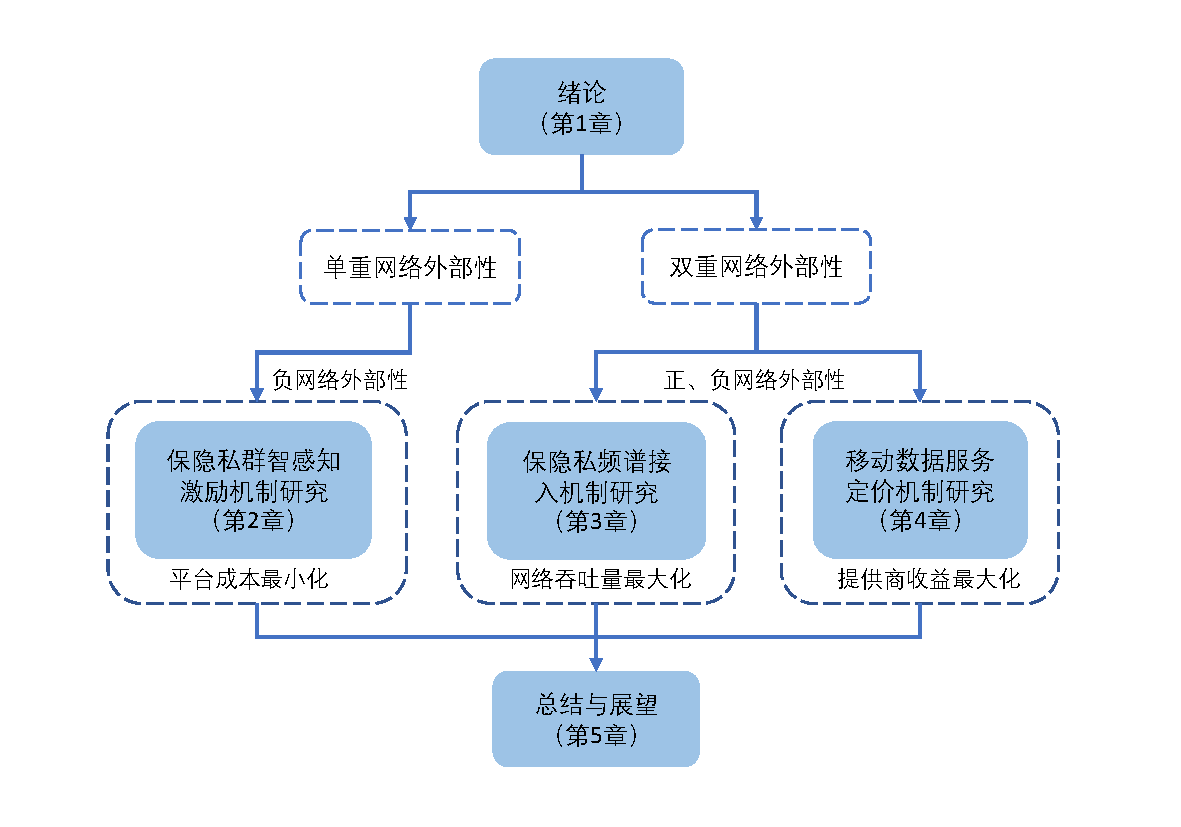
\includegraphics[width=1.05\textwidth]{pic/jiegou2.pdf}
%\caption{全文组织结构图}
%\label{fig:the}
%\end{figure}

\subsection{研究重点}

本文主要研究以下三个问题:

第一、单重网络外部性下移动群智感知系统平台成本最小化研究。移动群智感知是移动大数据时代重要的数据采集方式,同时是移动网络用户个人数据隐私保护的重点。本文以数据隐私保护下群智感知系统平台成本最小化为效用优化目标,提出研究一种用于移动群智感知中隐私数据聚合的拍卖框架。由于移动用户的感知能力和提供数据的隐私成本是有差异的,充当拍卖者角色的感知平台的主要挑战在于选择合适的参与用户,为此本文为他们设计用于隐私保护的数据噪声分布,使得数据聚合结果达到准确性指标,同时用户的隐私得到保护并获取足够的奖励。同时,本文提出一种允许用户进行本地数据加噪的方案。其中用户所允许添加的噪声分布由感知平台决定,其数据隐私保护程度可以使用差分隐私的量化指标进行衡量。本文分析揭示了该数据加噪的方案下用户间所存在的{\kaishu 负网络外部性}效应,并根据用户对于隐私保护级别的偏好分成“消极隐私保护”和“积极隐私保护”两种情形进行问题的建模与求解。在“消极隐私保护”情形中当平台可以通过支付奖励充分补偿用户的隐私损失时,用户即愿意参与并提供感知数据。而在更具一般性的“积极隐私保护”情形中,参与用户对其数据隐私保护级别存在固有要求,仅当要求满足时才同意参与任务。进一步,基于问题隐藏的单调性特性,本文分别针对两种情形设计了具有诚实性、个体理性,计算效率高的激励机制,以近似地最小化感知平台用于购买用户数据的成本,同时满足对于聚合结果准确性的要求。最后,通过理论分析结合充分的仿真实验验证所提出方案的可行性。

第二、双重网络外部性下频谱共享网络吞吐量最大化研究。在数据库辅助频谱共享场景中,便携式移动设备与用户的强关联性,对移动设备的定位攻击给用户带来了位置隐私保护方面的担忧。本文为移动用户设计了为信号传输功率水平添加随机扰动的策略,以削弱基于RSS的潜在位置隐私攻击的威胁。另一方面,虽然频谱共享网络中用户之间的物理信号干扰({\kaishu 负网络外部性})会给网络整体性能带来负面影响,但用户之间社交关联引入的社交效应({\kaishu 正网络外部性})给系统效用带来了一定的提升空间。本文中,每个次级用户在进行频谱接入决策时,把包含其社交好友效用的“社交群体效用”作为自己的优化目标。进一步,本文将这种隐私保护下的具有社交意识的频谱共享问题建模成一个随机信道选择博弈。博弈中次级用户作为策略性的玩家动态调整其策略,以最大化其社交群体效用。针对提出的博弈模型,本文还设计了一个基于无悔规则的双时间尺度分布式学习算法,并证明其几乎可以肯定收敛至博弈的相关均衡集合。仿真实验得到的数值结果证实了所提出方案的可行性。

第三、双重网络外部性下移动数据服务提供商收益最大化研究。
在竞争性数据服务市场中多个服务提供商通过定价策略的制定以最大化自身收益。市场中移动用户的数据消费行为同时受到两方面因素的影响:社交效应({\kaishu 正网络外部性})和拥塞效应({\kaishu 负网络外部性})。为了分析移动用户和服务提供商之间的策略互动,本文设计了一个两阶段的斯塔克伯格博弈,分别由第一阶段的提供商博弈和第二阶段的用户博弈组成。针对用户博弈,本文刻画了均衡解的特征并建立了它的唯一性。对于提供商博弈,分析表明,在提供商行为理性以及提供商行为有限理性的情形下,混合策略均衡解均是有保证的。进一步,本文提出了一种分布式学习算法,用于寻求提供商博弈的混合策略均衡解。最后,数值仿真结果对于正网络外部性和负网络外部性如何影响系统性能的提供了见解,并验证了提供商有限理性行为对其收益所产生的负面影响。


%第二章考虑了数据隐私保护下群智感知系统平台成本最小化问题,提出了一种用于移动群智感知中隐私数据聚合的拍卖框架。由于移动用户的感知能力和提供数据的隐私成本皆有所差异,充当拍卖者角色的感知平台的主要挑战在于选择合适的参与用户,并针对性地为他们设计用于隐私保护的数据噪声分布,使得数据聚合结果达到准确性指标,同时用户的隐私得到保护并获取足够的奖励。本文提出了一种允许用户进行本地数据加噪的方案。其中用户所允许添加的噪声分布由感知平台决定,其数据隐私保护程度可以使用差分隐私的量化指标进行衡量。本文揭示了用户间所存在的{\kaishu 负网络外部性}效应,并根据用户对于隐私保护级别的偏好分成“消极隐私保护”和“积极隐私保护”两种场景进行问题的建模与求解。在“消极隐私保护”场景中当平台可以通过支付奖励充分补偿用户的隐私损失时,用户即愿意参与并提供感知数据。而在更具一般性的“积极隐私保护”场景中,参与用户对其数据隐私保护级别存在固有要求,仅当要求满足时才同意参与任务。基于问题隐藏的单调性特性,本文分别针对两种场景设计了具有诚实性、个体理性,计算效率高的激励机制,以近似地最小化感知平台用于购买用户数据的成本,同时满足对于聚合结果准确性的要求。我们通过理论分析结合充分的仿真实验验证了所提出的方案。
%
%第三章考虑了位置隐私保护下具有社交意识的网络吞吐量最大化问题。在数据库辅助频谱共享的场景中,由于便携式移动设备与用户的强关联性,对移动设备的定位攻击给用户带来了位置隐私保护方面的担忧。本文中移动用户对信号传输功率水平添加随机扰动,以削弱基于RSS的潜在位置隐私攻击的威胁。另一方面,虽然用户之间的物理信号干扰({\kaishu 负网络外部性})会给网络整体性能带来负面影响,但用户之间社交关联引入的社交效应({\kaishu 正网络外部性})给系统效用带来了一定的提升空间。本文中,每个次级用户在进行频谱接入决策时,把包含其社交好友效用的“社交群体效用”作为自己的优化目标。进一步,本文将这种隐私保护下的具有社交意识的频谱共享问题建模成一个随机信道选择博弈。博弈中次级用户作为策略性的玩家动态调整其策略,以最大化其社交群体效用。我们针对博弈模型设计了一个基于无悔规则的双时间尺度分布式学习算法,并证明其几乎可以肯定收敛至博弈的相关均衡集合。数值结果证实,隐私保护级别越高,网络吞吐量的下降就越显着。
%
%第四章考虑了服务提供商收益最大化问题。在竞争性数据服务市场中多个服务提供商通过定价策略的制定以最大化自身收益。市场中移动用户的数据消费行为同时受到两方面因素的影响:社交效应({\kaishu 正网络外部性})和拥塞效应({\kaishu 负网络外部性})。为了分析移动用户和服务提供商之间的策略互动,本文设计了一个两阶段的斯塔伯格博弈,分别由第一阶段的提供商博弈和第二阶段的用户博弈组成。针对用户博弈,本文刻画了均衡解的特征并建立了它的唯一性。对于提供商博弈,分析表明,对于提供商行为理性的场景以及提供商行为有限理性的场景,混合策略均衡解均是有保证的。进一步,本文提出了一种分布式学习算法,用于寻找提供商博弈的混合策略均衡解。最后,数值仿真结果对于正网络外部性和负网络外部性如何影响系统性能的提供了见解,并验证了提供商有限理性行为对其收益所产生的负面影响。


%最后,第六章对全文进行了总结,并提出了未来可能的研究方向。

\subsection{本文结构}

本文共分六章及附录。第一章为绪论,主要是首先介绍了移动网络的发展及其效用优化的重要性、分析了移动网络的网络外部性特征和有关研究进展,概述了本文选定研究主题以及研究视角的思考;接着分析综述了近些年国内外涉及与本文中移动网络效用优化场景相关领域的研究现状,以及有待研究的问题;最后阐述了本文的研究思路和主要内容。第二章主要介绍本文研究中所用到的基础理论工具,包括博弈原理、拍卖机制设计理论及展望理论等相关理论的概念、思想和模型,以及在本文研究中的应用及其体会。第三章、第四章、第五章是本文研究的主体,分章阐述移动网络三个场景中的效用优化和机制设计改进方案及其算法的分析研究过程和结论,其中第二、三章中的相关定理、引理和推论的推导证明另列为本文的附录\ref{sec:appA}、附录\ref{sec:appB}。第六章是对本文的总结和展望,概括了研究重点内容及其成果,分析了可能产生的主要贡献,并提出未来可能的研究方向及有关问题。全文的基本思路和组织架构如图\ref{fig:the}所示。

\begin{figure}[t]
\centering
\includegraphics[width=1.05\textwidth]{pic/jiegou2b.pdf}
\caption{全文组织结构图}
\label{fig:the}
\end{figure}

\chapter{非合作博弈与拍卖机制相关理论基础}

\textbf{本章摘要:} 
本章分别介绍了与本文相关的非合作博弈的基本概念,包括动态博弈的分类、斯塔克伯格博弈模型;同时介绍了与本文相关的拍卖机制设计理论;最后介绍了行为经济学中展望理论框架下博弈中个体的非完全理性模型。


\textbf{关键词:}非合作博弈;拍卖机制设计;展望理论

%\section{引言}

\section{非合作博弈相关理论基础}\label{sec:game}
博弈论(Game Theory)是研究理性个体互动决策的理论,源于应用数学领域,后又在经济学、计算机科学、管理学等学科领域得到进一步理论发展与广泛应用。根据博弈参与者能否形成约束性协议,博弈可分为合作博弈和非合作博弈\cite{osborne,Fudenberg}。一般认为,当参与者根据自身利益,无法与其他参与者就行动选择达成约束性协议而独立作出决策时,该博弈模型属于非合作博弈\cite{osborne}。

\subsection{非合作博弈的表征}

非合作博弈的表征形式包含三类,即策略博弈(Strategic game)、延展博弈(Extensive game)和联合博弈(Coalitional game),在本文中我们的讨论主要是策略博弈\cite{osborne}。策略博弈是一种典型的静态博弈,其中所有的参与者同时进行行动,在数学上有如下的定义:
\begin{df}[策略博弈]
一个策略博弈可以由一个有序三元组定义:
\begin{equation}
\mathcal{G}=(\mathcal{V},\{\mathcal{S}_i\}_{i\in\mathcal{V}},\{u_i\}_{i\in\mathcal{V}})
\end{equation}
其中
\begin{enumerate}
\item $\mathcal{V}=\{1,\cdots,N\}$为一个有限的参与者集合。
\item $\mathcal{S}_i$为表示参与者$i$可行策略空间的一个非空策略集合。
\item $u_i: \mathcal{S}\rightarrow  \mathbb{R}$代表参与者$i$的收益,其中$\mathcal{S}\triangleq\prod_i\mathcal{S}_i$代表所有参与者的策略空间。
\end{enumerate}
\end{df}
根据上述定义,一个策略博弈模型可以由参与者集合、行为集合和参与者在不同行为交互情况下的收益集合三部分来表征。博弈的参与者其中当策略集合$\mathcal{S}_i$为由参与者$i$所有可选行动组成的集合$\mathcal{A}_i=(a_{i1},a_{i2},\cdots)$时,元素$s_i\in\mathcal{S}_i$也被称为纯策略(Pure-strategy)。对应地,当策略集合中的元素$s_i\in\mathcal{S}_i$对应于参与者$i$定义在可选行动集合$\mathcal{A}$上的一个策略分布$\pi_i$时,元素$s_i\in\mathcal{S}_i$则被称为一个混合策略(Mixed-strategy)。进一步,我们令向量$s_{-i}=[s_j]_{j\neq i}\in\mathcal{S}_{-i}$为除参与者$i$外其余参与者的策略向量,其中$\mathcal{S}_{-i}\triangleq\prod_{j\neq i}S_j$表示除参与者$i$外其余参与者的策略空间。


\subsection{博弈的均衡}\label{sec:neconcept}

最优响应是指博弈中参与者在其他参与者策略已知或可预测条件下,给自身带来最大化收益的策略\cite{osborne,Fudenberg},数学上定义如下:
\begin{df}[最优响应]
对于策略博弈$\mathcal{G}=(\mathcal{V},\{\mathcal{S}_i\}_{i\in\mathcal{V}},\{u_i\}_{i\in\mathcal{V}})$中的任意参与者$i\in\mathcal{V}$,及任意$s_{-i}\in\mathcal{S}_{-i}$,参与者$i$的最优响应为
\begin{equation}
B_i(s_{-i})=\arg\max_{s_i\in\mathcal{S}_i}u_i(s_i,s_{-i})
\end{equation}
\end{df}

当一个策略博弈中的每个参与者都将最优响应作为自己的行动时,该博弈即可达到均衡状态,对应的所有参与者的策略即为纳什均衡(Nash Equilibrium)\cite{Nash1951},其定义如下:
\begin{df}[纳什均衡]
假设对于策略博弈$\mathcal{G}=(\mathcal{V},\{\mathcal{S}_i\}_{i\in\mathcal{V}},\{u_i\}_{i\in\mathcal{V}})$中每个个体$i\in\mathcal{V}$,若满足
\begin{equation}\label{}
u_{i}(s_{i}^*,s_{-i}^*)\ge u_{i}(s_{i},s_{-i}^*),~\forall s_i\ne s_i^*.
\end{equation}
则纯策略$s^*=(s_{1}^*,\cdots,s_{N}^*)\in\mathcal{S}$是一个(纯策略)纳什均衡。
\end{df}
对于使用纳什均衡作为策略博弈的解,较为广泛的一种解释是因为纳什均衡对应于博弈的一个稳定状态,在这个状态上任何参与者都无法通过单方面改变其策略以获得更高的收益,因而没有偏离其当前均衡策略的动机。然而由于一个策略博弈并不能保证其纯策略纳什均衡的存在,因而出现了由纳什均衡衍生出的一些其他均衡概念,这些均衡解的出现方便了对于博弈模型均衡状态的分析。例如,当博弈中参与者所使用的策略$s_i$对应为一个混合策略$\pi_i\in\Delta\mathcal{A}$时,博弈相应的均衡即成为混合纳什均衡\cite{Fudenberg,Lasaulce2011}。
\begin{df}[混合纳什均衡]
假设对于策略博弈$\mathcal{G}=(\mathcal{V},\{\mathcal{S}_i\}_{i\in\mathcal{V}},\{u_i\}_{i\in\mathcal{V}})$中每个个体$i\in\mathcal{V}$,若满足
\begin{equation}\label{}
u_{i}(\pi_{i}^*,\pi_{-i}^*)\ge u_{i}(\pi_{i},\pi_{-i}^*) + \epsilon,~\forall \pi_i\ne\pi_i^*.
\end{equation}
则混合策略均衡$\pi^*=(\pi_{1}^*,\cdots,\pi_{N}^*)\in\Delta\mathcal{A}$是一个混合纳什均衡。
\end{df}

一个混合策略是对于参与者所有可能行为的随机化选择,因此不难理解纯策略纳什均衡是混合策略纳什均衡的一个特例。进一步我们还可以通过设定一个阈值$\epsilon$,更具一般性地得到对于混合策略纳什均衡的一个近似,即$\epsilon$-纳什均衡\cite{Fudenberg,Lasaulce2011}:
\begin{df}[$\epsilon$-纳什均衡]
假设对于策略博弈$\mathcal{G}=(\mathcal{V},\{\mathcal{S}_i\}_{i\in\mathcal{V}},\{u_i\}_{i\in\mathcal{V}})$中每个个体$i\in\mathcal{V}$,若满足
\begin{equation}\label{}
u_{i}(\pi_{i}^*,\pi_{-i}^*)\ge u_{i}(\pi_{i},\pi_{-i}^*) + \epsilon,~\forall \pi_i\ne\pi_i^*.
\end{equation}
则混合策略均衡$\pi^*=(\pi_{1}^*,\cdots,\pi_{N}^*)\in\Delta\mathcal{A}$是一个$\epsilon$纳什均衡。
\end{df}

当博弈处于$\epsilon$-纳什均衡状态时意味着任意参与者通过单方面偏离博弈均衡策略只能获得不超过$\epsilon$的收益增加。
%由于$\epsilon$-纳什均衡属于混合纳什均衡,因此一个有限博弈可以确保存在一个$\epsilon$-纳什均衡。
以上所介绍的纳什均衡相关概念中均默认要求参与者独立地完成策略(纯策略或混合策略)的选择。在一些情况下,博弈参与者的策略之间可能存在相关性。例如,当博弈开始前参与者之间存在一定的信息交互,或博弈存在一个“协调者”可以向每个参与者进行策略建议(参与者可以不接受)。在这种设定下,博弈的稳态可由相关均衡(Correlated Equilibrium)\cite{Aumann}来刻画:
\begin{df}[相关均衡]
我们称定义在$\Delta\mathcal{S}$上的联合概率分布$\pi^*$为一个非合作博弈$\mathcal{G}=(\mathcal{V},\{\mathcal{S}_i\}_{i\in\mathcal{V}},\{u_i\}_{i\in\mathcal{V}})$的一个相关均衡(CE),如果$\forall i\in\V$,$\forall t_{i},s_i\in\mathcal{S}_i$,$t_i\neq s_i$,个体收益$u_i$满足以下不等式,
%A probability distribution $\pi^*$ on $\Delta\mathcal{M}$ is a socially-aware correlated equilibrium (CE) of game $\Gamma$ if, $\forall n\in\V$, $\forall a_{n,i},a_{n,j}\in\mathcal{M}_n$, the expected group utility satisfies the following,
\begin{equation}
\sum_{s_{-i}\in\mathcal{S}_{-i}}\pi^*(s)\left[u_i(t_i,s_{-i})-u_i(s)\right]\leq0.
\end{equation}
\end{df}

在相关均衡状态上,任何参与者都无法通过单方面偏离“协调者”的建议而获得收益的提升。从以上定义可以看出,一个混合纳什均衡可以被看作为一个相关均衡的特例,因而相关均衡在实际中较混合纳什均衡更易出现。
%在一些不存在纯纳什均衡的有限博弈中,我们可以转而使用混合纳什均衡和相关均衡来研究分析博弈的均衡状态。
本文中第四章使用了相关均衡(CE)来刻画移动设备的频谱选择均衡策略,本文的第五章则分别使用了纳什均衡和$\epsilon$-纳什均衡的概念对于移动用户和服务提供商的均衡策略进行刻画。博弈论中还有其他的均衡概念,例如占优策略均衡(Dominant strategy Equilibrium)和子博弈精炼均衡(Subgame Perfect Equilibrium)和均衡等,由于他们在本文中没有涉及,这里我们不进行详细介绍。

博弈论中对于博弈均衡解的研究通常包括对于均衡解存在性、唯一性以及均衡解效率上的分析。从数学上讲,证明纳什均衡的存在等价于证明一个定点问题(Fixed-point problem)解的存在性。因此众多关于均衡存在证明的工作都基于对于定点定理的推导。本节仅介绍一个与本文相关的纳什均衡存在性的结论\cite{Nash48}。

%\begin{thm}(有限博弈中纯纳什均衡的存在性)
%在理想信息前提下,每一个有限博弈存在至少一个纯纳什均衡。
%\end{thm}

\begin{thm}[有限博弈中混合纳什均衡的存在性]
若策略博弈$\mathcal{G}=(\mathcal{V},\{\mathcal{S}_i\}_{i\in\mathcal{V}},\{u_i\}_{i\in\mathcal{V}})$满足参与者集合与对应的策略集合为有限集合,则称该博弈为有限博弈(Finite Game),且该博弈至少存在一个混合纳什均衡。
\end{thm}

博弈均衡解的唯一性与均衡解的质量相比存在性分析更为复杂,且通常需要在特定问题模型中针对具体问题进行具体分析,因此不在这里进行介绍。

%当一个动态博弈具有有限的状态空间与动作空间时,该动态博弈至少存在一个策略均衡。而通常一个存在均衡的动态博弈会同时拥有多个均衡状态。

\subsection{动态博弈}
非合作博弈模型可以被分为静态博弈与动态博弈两类\cite{osborne,Fudenberg,han2012game}。通常,我们认为静态博弈中参与者拥有对于博弈确定的认知,包括对于信息和行为的假设,且这些认知不随博弈进行而改变,参与者则仅需基于已有的关于其他参与者信息行为的假设进行一次性的行动。前几节中我们正是在静态博弈的范畴下对于策略博弈的表征形式与均衡概念进行了相关的讨论。相比于静态博弈,动态博弈中通常假设参与者可以从过往的行动和策略中提取有用信息,并用于当前与未来行动与策略的制定。动态博弈模型主要包括以下几类:

\begin{itemize}
\item {\heiti 重复博弈:}顾名思义,一个标准的重复博弈包含对于同一静态博弈有限或无限次的重复进行,其中参与者通过重复的策略交互以求最大化自身长期收益,会产生静态博弈中所不存在的合作与惩罚的现象。
\item {\heiti 随机博弈:}随机博弈则较重复博弈更具一般性。参与者的即时收益不单取决于当前参与者的行为,同时取决于环境当前的状态。随机博弈中又可细分为共同状态(Common states)随机博弈和个体状态(Individual states)随机博弈。共同状态随机博弈中博弈环境对于所有参与参与者相同,而在个体状态随机博弈中,每个参与者可以处于不同的博弈环境状态。
\item {\heiti 差分/差异博弈:}与重复博弈和随机博弈不同,差分/差异博弈则在时间上是连续的。通常,差分博弈中的状态进化规则(例如一个确定性的或者随机的差分方程)。差异博弈则是对于差分博弈的离散化,当处于极限情况下时即等价于差分博弈。差异博弈可被看作为介于差分博弈与随机博弈之间的一种动态博弈类型。
\item {\heiti 演化博弈:}演化博弈通常涉及到大规模的用户,侧重于研究用户间交互所导致的群体演化的研究。其应用起源于生物学与社会学中。
\end{itemize}

与静态博弈不同,动态博弈在建模中需考虑两个较为关键的问题:首先,如何对参与者所处的动态环境进行建模。一些差分方程用于从数学上刻画参与者所处环境的动态特性。其次,如何对参与者的目标进行建模。在大部分场景下,参与者的收益需要根据动态环境调整为长期的期望收益。本文的研究内容主要涉及到重复博弈与个体状态随机博弈。

\subsection{斯塔克伯格博弈}
斯塔克伯格博弈是由H. Stackelberg提出的一种典型的重复博弈,属于完全信息非合作博弈的范畴。在斯塔克伯格博弈中,博弈的参与者分为领导者(Leader)和跟随者(Follower),博弈分为两个阶段。在第一阶段中,领导者首先行动,跟随者随后行动。在一些斯塔克伯格博弈场景中,可能出现领导者和跟随者分别同时包含多个个体的情况,则问题可被看成是两层的优化问题。在博弈的上层,领导者们在了解跟随者的策略及收益函数的情况下,选择最优策略以最大化自身效用。在博弈的下层,跟随者在观察到领导者的行为后,通过非合作博弈选择其最佳对策。斯塔克伯格博弈的均衡可由逆向归纳法(Backward Induction)得到。该模型在竞争型市场商品定价和产量决策中具有重要应用价值。

%\subsection{基于学习的博弈均衡求解}
%
%最优响应动态和强化学习算法都是可以帮助博弈达到纳什均衡的动态
%
%在最优响应动态中,参与者需要能够观察到其他参与者的行为。而使用基于强化学习的算法则仅要求已知博弈每一个阶段时参与者的即时收益值。
%
%收敛,以概率1收敛。


\section{拍卖机制设计相关理论}\label{sec:mech}

机制设计理论(Mechanism Design),源自于经济学家L. Hurwicz在上世纪六七十年代的开创性工作。它所研究的即是如何通过逆向工程的方法根据给定的效用优化目标设计相应的市场机制和博弈规则\cite{Nisan07}。当系统按照所设计机制运行时,即使当系统管理者和参与个体之间存在信息不完全和信息不对等的情况时,个体依然可以获得足够的激励参与到系统中,而系统可以达到一些既定的性能要求。在一些资源优化分配的机制设计场景中,较为常用的一类激励机制是拍卖机制。

\subsection{拍卖机制基本概念与原理}
作为博弈论的一个分支,拍卖模型与博弈模型一样在众多涉及到资源分配的领域有着较为广泛的应用。从理论上讲,拍卖机制实现的是在买卖双方信息不对等的情况下以一种竞价的方式,完成实际或虚拟的物品经由拍卖者(Auctioneer)在买家(Buyer)和卖家(Seller)之间的交换\cite{Nisan07}。

%对于任意给定的一个经济或社会目标,在自由选择、自愿交换、信息不完全对等的决策条件下,能否设计以及怎样设计出一个经济机制,使经济活动参与者的个人利益和设计者既定的目标一致是至关重要的。从研究路径和方法来看,与传统经济学在研究方法把市场机制作为已知,研究它能导致什么样的配置有所不同,机制设计理论把社会目标作为已知,试图寻找实现既定社会目标的经济机制。

%通常认为,评价某种经济机制优劣的基本标准有三个:资源的有效配置、信息的有效利用以及激励相容。资源有效配置通常采用帕累托最优标准,有效利用信息要求机制运行需要尽可能低的信息成本,激励相容要求个人理性和集体理性一致。

根据拍卖的供需匹配类型、资源(商品)属性以及拍卖规则,拍卖模型可以被进行如下的类型划分:
\begin{itemize}
\item 供需匹配类型:当拍卖模型中多个买家从一个卖家处竞得拍卖物品时,卖家为拍卖者,该拍卖为正向拍卖。相反,当拍卖模型中存在一个买家向多个卖家购得拍卖物品时,买家为拍卖者,该拍卖为反向拍卖(Reverse auction)。当拍卖模型中同时存在多个卖家和买家时,买家和卖家需分别向一个第三方拍卖者进行报价,以完成物品的拍卖,该拍卖称为双向拍卖(Double auction)。
\item 物品属性:一个拍卖模型可以依据被拍卖物品的属性进行分类。例如,按物品种类分为单物品拍卖或组合拍卖(Single-item/ Combinatorial),按照供需方对物品的需求分为单件需求拍卖或多件需求拍卖(Single-minded/Multi-minded),按同一物品份数分为单件物品拍卖或多件物品拍卖(Single-unit/ Multi-unit)。
\item 拍卖规则:按照拍卖中报价的原则,一个拍卖机制可以被分为公开报价或密闭报价拍卖(Open-bid auction/Sealed-bid auction),公开报价博弈中报价可序惯性地进行,报价是公开的。而密闭报价拍卖的出价是同时性的,报价者提交密封式的竞价并且报价最高者赢得物品可。根据奖励方式的不同,密闭报价可进一步分为第一价格(First-price)拍卖与第二价格(Second-price)拍卖两类。不同于第一价格拍卖中奖励额设为赢家的报价,第二价格拍卖中,奖励额设为除赢家外剩余报价者中的最高(反向博弈中的最低)报价。
\end{itemize}
%\subsection{激励机制的性质}
尽管拍卖模型的类型繁多,但每一个拍卖机制都包括三个不可缺少的阶段:报价(Bidding)、赢家确定(Winner determination)和奖励确定(Price determination)。简单来说,一个拍卖机制的设计就是在报价规则形式确定的情况下,通过设计赢家确定与奖励确定的规则,使得激励机制在运作中满足以下基本要求:
\begin{itemize}
\item \textbf{诚实性(Truthfulness)}:参与用户无法通过不诚实的报价行为获取收益上的提升。
\item \textbf{个体合理性(Individual Rationality)}:每个参与用户收到的奖励不低于其隐私损失。
\item \textbf{计算高效性(Computational Efficient)}:赢家的确定与奖励的确定需要达到多项式时间复杂度。
\item \textbf{近似最优性(Approximation)}:机制运行所得到的效用近似接近于目标最优值。
\end{itemize}
%由以上定义可看出,当处于机制均衡状态时每个个体可获得非负的效用,则该机制具备个体合理性的性质。由于激励机制无法强迫个体的参与,因此个体理性是对一个有效的激励机制最基本的要求。

%单一变量机制设计问题,其中每个竞价者只有一个隐私数值


\subsection{反向拍卖机制}

本文主要关注的是反向拍卖机制。与常规的正向拍卖不同,反向拍卖机制中一般存在着一个买家和多个提供同类物品的卖家,买家作为拍卖者从卖家处购得物品。因此反向拍卖有时也被称为采购拍卖(Procurement auction)\cite{Nisan07}。在反向拍卖中,买家首先会给出所要获得的商品,然后由卖家对自己所拥有的符合买家需求的商品进行报价(Bidding),买家随后根据卖家的报价以及商品的价值选择获胜的卖家集合以及给予他们的相应奖励。假设有一系列的物品$[n]=\{1,\cdots,N\}$和一个买家。每一个物品对应一个卖家$i$,并且对应于一个真实价值$c_i\in\mathbb{R}^+$以及一个卖家的报价$b_i\in\mathbb{R}^+$。我们令一个反向拍卖机制$\mathcal{M}=(f, p)$包含一个分配函数$f: \mathbb{R}_{+}^{N} \rightarrow 2^{[n]}$和一个支付函数$p: \mathbb{R}_{+}^{n} \rightarrow \mathbb{R}_{+}^{n}$。其中分配函数基于卖家报价得到一个赢家集合$\mathcal{S}$,支付函数$p$返回对于每个卖家$i$的奖励$p_i$。我们令$\mathbf{s}=\{s_1,\cdots,s_N\}$为刻画赢家集合$\mathcal{S}$的向量,有$\forall i\in\mathcal{S}, s_i=1$和$\forall i\notin\mathcal{S}, s_i=0$。我们令价值函数$V(S): 2^{[n]} \rightarrow \mathbb{R}_{+}$代表买家从购得物品中可获得的价值。在数学上,拍卖机制的个体合理性可以被描述为:$p_i\geq s_i\cdot b_i$以及当$s_i=0$时,$p_i=0$。机制的诚实性可以被描述为:对于任意卖家$i\in[n]$,以及卖家报价$\{b_1,\cdots,b_N\}$,有$p_{i}-s_{i} \cdot b_{i} \leq p_{i}^{\prime}-s_{i}^{\prime} \cdot c_{i}$,其中$p_{i}^{\prime},s_{i}^{\prime}$为卖家$i$使用真实报价$c_i$时得到的拍卖结果。

基于以上的设定,我们在讨论机制的诚实性时可以直接应用Myerson最优机制定理\cite{Myerson1981}:
\begin{thm}
在单变量机制设计中,机制$\mathcal{M}=(f, p)$具有诚实性当且仅当以下两个条件得到满足:
\begin{enumerate}
\item $f$是单调的:对于所有$i \in[n]$且$b_{i}^{\prime} \leq b_{i}$,如果对于任意$b_{-i}$,有$i\in f\left(b_{i}, b_{-i}\right)$,则有$i \in f\left(b_{i}^{\prime}, b_{-i}\right)$。
\item 赢家被支付阈值奖励:$p_i = \inf \left\{c_{i}: i \notin f\left(c_{i}, c_{-i}\right)\right\}$。
\end{enumerate}
\end{thm}
基于反向拍卖的基本设定,我们接下来介绍一类典型的反向拍卖机制,预算可行机制。


\subsubsection{预算可行机制}
预算可行机制是一类特殊的是反向博弈中的,由Singer\cite{Singer}于2010年首次提出。它在基本反向博弈的模型基础上添加了一个对于买家支付的预算$B$,对支付给赢家的总奖励进行了约束,即$\sum_{i} p_{i} s_{i} \leq B$。Singer对于买家价值函数$V$属于子模函数的情况进行了研究。
\begin{df}
如果一个价值函数$V: 2^{[n]} \rightarrow \mathbb{R}^{+}$满足以下两个条件:
\begin{enumerate}
\item 如果$S \subseteq T$则$V(S) \leq V(T)$.
\item $V(S \cup\{i\})-V(S) \geq V(T \cup\{i\})-V(T), \quad \forall S \subseteq T$.
\end{enumerate}
则$V$是一个非降子模函数。
\end{df}

对于以单调子模函数为优化目标的机制设计,我们基于卖家对于价值函数边际贡献与其成本的比值对卖家进行递归排序,即$i+1=\arg\max_{j\in V/S_i}\frac{V(S\cup\{i\})-V(S)}{c_j}$,其中$S_i=\{1,\cdots,i\}$,$S_0=\emptyset$。令$V_i=V(S\cup\{i\})-V(S)$,则在子模的条件下,可以得到:
\begin{equation}
V_{1} / c_{1} \geq V_{2} / c_{2} \geq \ldots \geq V_{N} / c_{N}.
\end{equation}
其中$V\left(S_{k}\right)=\sum_{i \leq k} V_{i}$。
使用基于比例分配规则的贪婪算法,我们可以得到拍卖机制的阈值奖励$\theta'_i$为
\begin{equation}
\theta_{i}^{\prime}=\min \left\{\frac{V_{i} \cdot B}{\sum_{i \in S} V_{i}}, \frac{V_{i} \cdot c_{k+1}}{V_{k+1}}\right\}
\end{equation}
同时满足诚实性和个体合理性的要求。本文中在第三章的机制设计研究中使用到了与预算可行机制的设计目标具有互补性的节俭机制。预算可行机制的目标是在预算约束存在情况下选择合适的赢家集合与支付以最大化价值函数,而节俭机制的目的则是在购得物品价值满足一定要求的情况下最小化买家的总支付。我们在节俭机制的设计中同样使用了以比例分配规则为核心思想的贪婪算法。

\section{展望理论中的个体有限理性模型}\label{sec:setup}
在移动网络中的机制设计和效用优化中,充分考虑各类运营主体特别是众多的不同用户的行为模型上的异质性是至关重要的。行为经济学(Behavioral Economics)对于个体的非完全理性行为有着广泛且深入的研究。1979 年,美国普林斯顿大学心理学教授丹尼尔·卡内曼和阿莫斯·特沃斯基提出了 “展望理论”(Prospect Theory)\cite{Kahneman},也有译为“前景理论”。与传统的期望效用函数理论(Expected Utility Theory)的理性个体假设不同,展望理论从实证研究出发,从人的心理特质、行为特征揭示了影响选择行为的非理性心理因素,认为大多数人在面临获利的时候是风险规避的、在面临损失的时候是风险喜好的,而对其对得失的判断往往根据参考点来做出决定的。因为该理论将来自心理学研究应用到经济学之中,尤其是在不确定情况下的人为判断和决策方面作出了突出贡献,并被普遍作为是决策论的期望理论之一,卡内曼教授获得了 2002 年度诺贝尔经济学奖。本节主要介绍本文第五章所涉及到的展望理论中的{\kaishu 概率失真效应}和{\kaishu 效用框架效应}。

\subsection{概率失真效应}
概率失真效应是展望理论的两个主要特征之一,其指现实中决策者倾向于看重小概率事件,但是看轻中等和大概率事件。具体而言,这种特性可以通过将客观概率$p$映射到主观概率的概率失真函数$w(p)$来刻画。使用较为广泛的概率失真函数有Prelec函数\cite{Prelec}:
%We consider two main features of Prospect Theory. The first one is the \emph{probability distortion effect}, which states that decision maker is prone to overweigh events with small probability, but underweight medium and large probability events. Specifically, this characteristic can be captured by a probability distortion function $w(p)$ that maps an objective probability $p$ to a subjective one. A widely used probability distortion function is the Prelec function \cite{Prelec}:
\begin{equation}\label{eq:distortion}
w(p)=\exp(-(-\ln p)^{\alpha}), 0<\alpha\leq 1,
\end{equation}
其中$p$是事件的真实概率,$\alpha$是概率失真参数,$w(p)$是对应的主观概率。图\ref{fg:dist_func}阐明了具有不同参数的概率失真函数(\ref{eq:distortion})。我们可以看到所有曲线在点$1/e$相交。此外,当$0\leq p < 1/e$时,函数是凸的,$w(p)<p$(即低估客观概率);而当$1/e\leq p<1$时,函数是凹的,我们有$w(p)\geq p$(即高估客观规律)。失真参数$\alpha$的值越小,则概率失真效应越明显。当$\alpha$设置为1时,该函数即变为客观概率。
%在这里我们考虑同类服务提供商,其主观评估可以通过(\ref{eq:distortion})中给出的具有相同$\alpha$取值的失真函数来表征。同时,我们假设服务提供商能够客观地评估自身的策略。因而在前景理论下,用户$k$对联合定价策略$\mathbf{p}\in\Delta\mathcal{P}$的评估可以表示为$\pi_k(p_k)w(\prod_{k'\in\K,k'\neq k}\pi_{k'}(p_{k'}))$。
%where $p$ is the real probability of an event, $\alpha$ is the probability distortion parameter, and $w(p)$ is the corresponding subjective probability. Fig. \ref{fg:dist_func} illustrates the probability distortion function (\ref{eq:distortion}) with different parameters. We can see that all the curves intersect at the point $1/e$. Besides, we have when $0\leq p < 1/e$, the function is convex, and $w(p)<p$ (under-weighting); when $1/e\leq p<1$, the function is concave, and we have $w(p)\geq p$ (over-weighting). A smaller value of distortion parameter $\alpha$ corresponds to a more significant probability distortion effect. When $\alpha$ is set to 1, the function reduces to the objective probability. In our work, we consider homogeneous service providers whose subjective evaluation can be characterized by the distortion function given in (\ref{eq:distortion}) with a same fixed value of $\alpha$. Meanwhile, we assume that service providers are able to evaluate their own strategies objectively. Thus, user $k$'s evaluation for a joint pricing strategy $\mathbf{p}\in\Delta\mathcal{P}$ under Prospect Theory can be expressed as $\pi_k(p_k)w(\prod_{k'\in\K,k'\neq k}\pi_{k'}(p_{k'}))$.
\begin{figure}
\centering
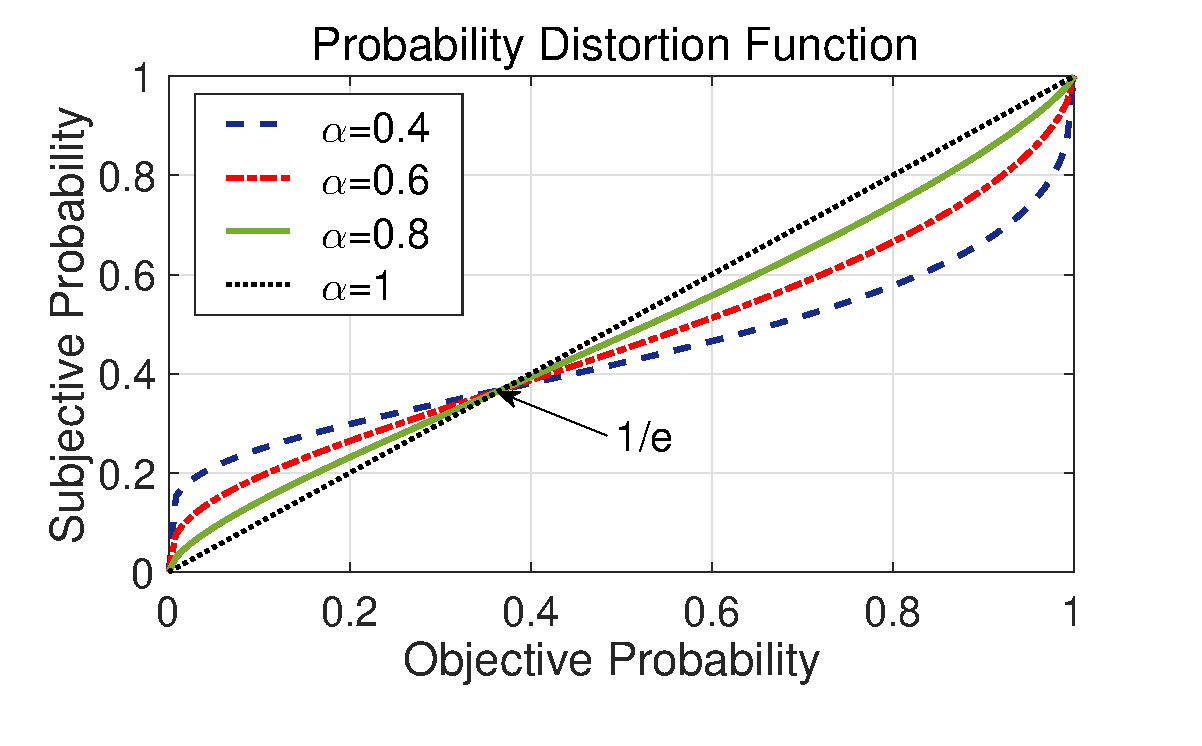
\includegraphics[scale=0.6]{./pic/dist_func.eps}
%\caption{Probability distortion functions under different distortion parameters $\alpha$.}\label{fg:dist_func}
\caption{失真参数$\alpha$不同取值下的概率失真函数。}\label{fg:dist_func}
\vspace{0.1cm}
\centering
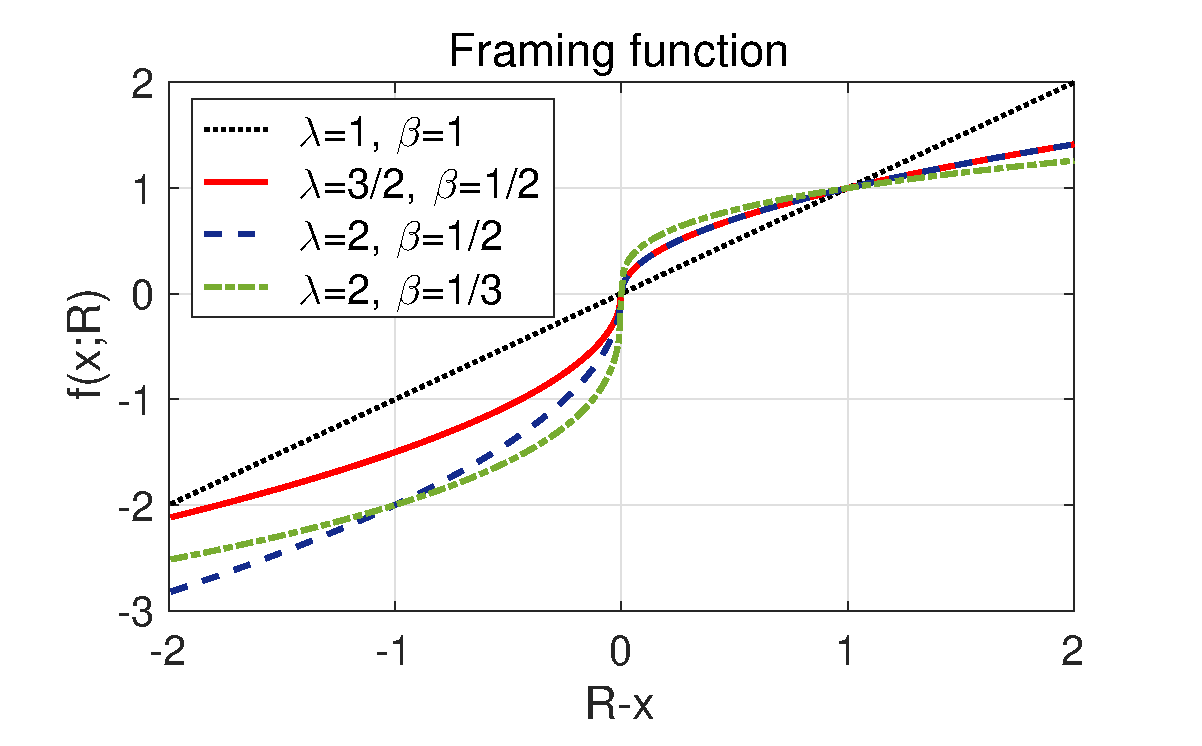
\includegraphics[scale=0.6]{./pic/fram_func.eps}
%\caption{Framing functions under different utility aversion parameters $\beta$ and loss penalty parameter $\lambda$.}\label{fg:fram_func}
\caption{不同效用规避参数$\beta$和损失惩罚参数$\lambda$下的框架函数。}\label{fg:fram_func}
\end{figure}

\subsection{效用框架效应}
我们考虑的展望理论的另一个特征是效用框架效应。此效应反映了每个服务提供商对自己的收益进行主观评估的实际情况。实际中,仅当其收入超过参照点$R$($R$无需等于零)时,每名用户才会将其视为收益增益,否则将视为收益损失。同样,在给定参考点$R$的情况下,S型单调框架函数$f(\cdot)$会进一步调整客观收入,其中函数在$v>R$侧为凹函数,而在$v<R$一侧是凸函数。此外,在$R$附近,收益损失比收益增益增长得更快,表明收益损失的边际效用大于收益增益的边际效用。常用的框架函数为Kahneman框架\cite{Kahneman},
%Another characteristic of Prospect Theory we considered is the \emph{utility framing effect}. This effect captures the practical situation where each service provider has subjective evaluation of her own payoff. In practice, each user might consider her payoff as a gain only if it is above a reference point $R$ (not necessarily equals zero), and consider it as a loss otherwise. Also, given the reference point $R$, the objective payoff is further tuned by a S-shaped monotone framing function $f(\cdot)$, which is concave at the side where $v>R$, and convex at the side where $v<R$. In addition, in the neighborhood of $R$, the losses loom larger than gains indicating that the marginal utility in losses is larger than in gains. In this work, we use a framing function based on the one proposed in \cite{Kahneman},
\begin{equation}\label{eq:framing}
f(x;R)=
\begin{cases}
(v - R)^{\beta}, &v\geq R\\
-\lambda(R-v)^{\beta}, &v<R
\end{cases}
\end{equation}
其中参数$0<\beta\leq 1$和$\lambda\geq 1$分别用于刻画风险规避和损失规避的因素。图\ref{fg:fram_func}展示了不同参数取值下的框架函数。特别地,当博弈参与者收入远离参照点时,$\beta$值越大,表示风险规避程度较小;$\lambda$值的增大则刻画了博弈参与者在客观上经历等同的收益的损失和增益时,所主观上体验到的损失要大于所体验到的增益。容易看出,当$\beta=\lambda=1$时,主观收益曲线与原始的客观收益曲线一致。
%我们假设每个服务提供商$k$基于式(\ref{eq:framing})来评估其收入。则在前景理论模型下,服务提供商$ k\in\K$的预期收入$z_k^{PT}$可写为
%where the parameters $0<\beta\leq 1$ and $\lambda\geq 1$ model the risk aversion and loss aversion respectively. Fig. \ref{fg:fram_func} illustrates the framing function with different parameters. In particular, a larger $\beta$ characterizes less degree of risk aversion when the player's payoff is away from the reference point; and a larger $\lambda$ captures the greater loss experienced by the player with her payoff being reduced by a certain amount, in comparison to the corresponding gain she experiences with the same amount of the payoff increase. It is easy to see that when $\beta=\lambda=1$, the subjective payoff boil down to the original objective payoff. We assume each service provider $k$ evaluate her revenue using (\ref{eq:framing}) with parameter $\beta_k$, and reference point $R_k, \forall k\in\K$. Under Prospect Theory model, the expected revenue $z_k^{PT}$ of service provider $k\in\K$ can be written as

%\begin{equation}\label{eq:PT}
%%\small
%z_{k}^{PT}(\pi_{k},\pi_{-k})=\sum_{\mathbf{p}\in \mathcal{P}}\pi_k(p_k)w\left(\prod_{k'\in\K,k'\neq k}\pi_{k'}(p_{k'})\right)f_k(v_k).
%\end{equation}
%
%我们将前景理论讨论下的定价博弈表示为$\mathcal{G}_P^{PT}\left(\mathcal{K},\Delta\mathcal{P},\{z_k^{PT}(R_k)\}_{k\in\mathcal{K}}\right)$,然后在下一节中重新讨论价格博弈的均衡解的存在。
%We denote the pricing game under Prospect Theory as $\mathcal{G}_P^{PT}\left(\mathcal{K},\Delta\mathcal{P},\{z_k^{PT}(R_k)\}_{k\in\mathcal{K}}\right)$, and revisit the existence of equilibrium solution for the pricing game in the next section.

展望理论在移动网络的效用优化问题研究中有着较大的应用价值。近些年,人们在解决一些移动网络中个体决策问题时,采用了展望理论对决策过程进行建模。 例如,Li等\cite{Tianming}研究了一种无线环境下的随机接入博弈,其中用户考虑了展望理论中的{\kaishu 概率失真效应}作用,策略性地确定其在冲突信道上的传输概率。Yu等\cite{Yu}研究了一种数据市场模型,模型中用户需要选择成为数据卖方还是数据买方,并确定交易的数据量。他们考虑了展望理论中的{\kaishu 概率失真效应}和{\kaishu 效用框架效应}对用户决策行为的影响,并将该问题表述为非凸优化问题。本文第五章中则运用了展望理论对无线服务提供商的有限理性行为进行刻画与建模。

%\section{本章小结}\label{chp2:sec:con}


\chapter{单重网络外部性下群智感知系统平台成本最小化研究}

\textbf{本章摘要:} 
本章提出了一种用于移动群智感知系统的保隐私数据聚合框架。其中用户为保护自身数据隐私,将本地数据加噪的感知数据提交给感知平台。这种由用户本地完成数据加噪的隐私保护方式给群智感知系统引入了{\kaishu 负网络外部性}的影响因素。
%:每个用户的隐私保护程度取决于聚合结果中的总噪声量,而总噪声量又取决于选择哪些移动用户以及这些用户所添加的噪声。
在这种网络外部性作用下,感知平台通过有限的市场力量,根据用户的隐私偏好和感知能力,选择合适的参与用户群组
%以最小化平台用于奖励用户的总成本,同时满足对于数据聚合结果的准确性要求。本章第3节首先考虑一种“消极隐私保护”的场景,即一旦平台可以通过奖励充分补偿用户的隐私损失,用户即愿意参与感知任务。
%本文使用解析表达式对问题的负网络外部性因素与隐藏的单调性特性进行了刻画与分析。
%,并基于此设计出一个具有诚实性、个体理性,计算效率高的激励机制。
%本章第4节将讨论扩展到一种“积极隐私保护”的场景,其中参与用户除了要求隐私成本得到补偿外,还对其所得到的数据隐私保护级别有固有的要求。
本章第3节和第4节分别针对“消极隐私保护”和“积极隐私保护”两种场景,提出了具备诚实性、个体合理性,计算高效性的拍卖激励机制,可以近似地最小化感知平台总成本同时满足数据聚合结果的准确性要求。本章通过理论分析结合充分的仿真实验对于提出的方案进行了验证。


%本章提出了一种用于移动群智感知保隐私数据聚合的拍卖框架,其中感知平台作为拍卖商征召移动用户完成感知任务并给予用户一定奖励以补偿其隐私损失。为保护自身数据隐私,移动用户将带有噪声的数据提交给感知平台。为确保数据聚合结果的准确性,感知平台只能通过有限的市场力量,即根据用户的隐私偏好和感知能力选择合适的感知用户群体,以此控制聚合数据中的噪声水平。这种由用户本地完成数据加噪的方式给群智感知系统引入了{\kaishu 负网络外部性}的影响因素:每个用户的隐私保护程度取决于聚合结果中的总噪声量,而总噪声量又取决于选择哪些移动用户以及这些用户所添加的噪声。本章研究了在这种{\kaishu 单重}负网络外部性作用下的拍卖激励机制设计。具体而言,本章第3节首先考虑一种“消极隐私保护”的场景,即一旦平台可以通过奖励充分补偿用户的隐私损失,用户即愿意参与感知任务并提供感知结果数据。本文通过解析表达式明确地描述了问题的负网络外部性因素与隐藏的单调性特性,并基于此设计出一个具有诚实性、个体理性,计算效率高的激励机制。本章第4节将讨论扩展到“积极隐私保护”的场景,即参与用户对其可获得的数据隐私保护级别有固有的要求。针对两种场景,本文提出的激励机制所确定的用户子集及相应奖励可以近似地最小化感知平台购买用户隐私数据的成本,同时满足对于数据聚合结果准确性的要求。本章通过理论分析结合充分的仿真实验对于提出的方案进行了验证。
%We develop an auction framework for privacy-preserving data aggregation in mobile crowdsensing, where the platform plays the role as an auctioneer to recruit workers for sensing tasks. The workers are allowed to report noisy versions of their data for privacy protection; and the platform selects workers by taking into account their sensing capabilities to ensure the accuracy level of the aggregated result. 
%%By leveraging the concept of differential privacy, we propose a differentially private data aggregation scheme that allows workers to generate noise by themselves while ensuring the differential privacy of their data in the aggregated result. Under this data aggregation scheme, the proposed framework introduces 
%In such an auction based framework, there exists externalities among workers' data privacy, because the data privacy of each worker depends on both her injected noise and the total noises from other workers that are selected to fulfill the task.

%Observe that when moving the control of data privacy from the data aggregator to the workers, the data aggregator has limited market power in the sense that it can only partially control the noise by judiciously choosing a subset of workers based on workers' privacy preferences. This introduces \emph{externalities} because the privacy of each worker depends on the total noise in the aggregated result that in turn relies on which workers are selected. 
%Specifically, we first consider a privacy-passive scenario where workers participate if their privacy loss can be adequately compensated by the rewards. 
%%To achieve a desirable accuracy level of the data aggregation in a cost-effective manner, we explicitly characterize the externalities.
%%, i.e., the impact of the noise added by each worker on both the data privacy and the accuracy of the aggregated result. 
%Further, we characterize the hidden monotonicity property of the problem, and determine the critical bid of workers, making it possible to design a truthful, individually rational and computationally efficient incentive mechanism. 

%We explicitly characterize the externalities and the hidden monotonicity property of the problem, making it possible to design a truthful, individually rational and computationally efficient incentive mechanism.
%We then extend the results to a privacy-proactive scenario where workers have individual requirements for their perceivable data privacy levels. Our proposed mechanisms for both scenarios can select a subset of workers to (nearly) minimize the cost of purchasing their private sensing data subject to the accuracy requirement of the aggregated result. We validate the proposed scheme through theoretical analysis as well as extensive simulations.

\textbf{关键词:}群智感知;数据隐私保护;拍卖理论;差分隐私
%\keywords{毫米波通信;Massive MIMO;整数规划}

\section{引言}

%\subsection{研究动机}
	近些年来,移动群智感知的兴起引发了人们的关注。作为一种颇具发展前景的无线传感网络应用,移动群智感知利用人们便携移动设备上的传感器来执行各种感知任务,其应用场景包括医疗保健,环境监测,室内定位和智能交通等\cite{sheng2013sensing}。 
	%Mobile crowdsensing arises as a promising sensing paradigm that leverages the sensing capability of human-carried mobile devices to perform various sensing tasks (e.g., healthcare, environment monitoring, indoor localization, and smart transportation) \cite{sheng2013sensing}. 
	通过将感知任务外包给公众,移动群智感知系统可以有效地收集细粒度的感知任务数据。然而另一方面,参与感知任务的任何个体不可避免地需要授予任务发布者一定权限以访问其感知数据,因而当感知数据本身具有敏感性且任务发布者为不可信第三方时,用户的隐私泄漏隐患便会暴露出来。这种隐私安全隐患已然成为除设备资源消耗(例如电池和计算能力)问题外,阻碍群智感知用户增长的主要因素。
	%By outsourcing the sensing tasks to the public crowd, mobile crowdsensing systems can collect fine-grained information effectively and efficiently. However, any individual involved in a sensing task inevitably authorizes the task agent a certain level of privilege to access her sensing data which may be sensitive, thereby giving rise to the privacy leakage when being released to an untrusted party. This becomes a key challenge hindering individuals (workers) from participation, other than the consumption of the limited system resources (e.g., battery and computing power) of their mobile devices.
	因此,移动群智感知的成功与否很大程度上取决于与隐私保护措施的激励机制设计与运用。
	%Therefore, the success of mobile crowdsensing hinges closely upon the design of efficient incentive mechanisms to stimulate workers' participation.
	
	大部分早期的移动群智感知系统激励机制设计\cite{yang2012crowdsourcing,feng2014trac,Zhao,wen2015quality,zhang2015incentivize,zhang2015truthful,jin2015quality,duan2012incentive,Shibo14,peng2015pay,cheung2015distributed,he2017exchange,gong2017truthful}仅考虑了参与用户的感知成本,而直到近些年才开始有更多研究工作将参与用户的隐私成本考虑进来。
	%Most of incentive mechanisms developed for mobile crowdsensing systems (e.g., \cite{yang2012crowdsourcing,feng2014trac,Zhao,wen2015quality,zhang2015incentivize,zhang2015truthful,jin2015quality,jin2016inception,zhang2016privacy,duan2012incentive,Shibo14,peng2015pay,cheung2015distributed,he2017exchange,gong2017truthful}) take into account only workers' sensing costs. Only a few recent works consider workers' privacy costs. 
	这其中大部分设计基于感知平台为可信第三方的理想假设,允许感知平台收集得到用户的原始数据后在数据聚合结果上进行加噪处理\cite{jin2016inception,zhang2016privacy}。该方式可以一定程度上解决公开聚合结果所导致的用户数据隐私泄露问题,然而参与用户自身缺乏对其数据隐私保护级别。尤其当感知平台可信度较低时,用户的参与度将大大降低。另有一些设计将平台与用户的交互建模为博弈问题\cite{wang2016value,wang2016buying},然而对于博弈均衡点质量控制上的挑战使得数据聚合结果的准确性难以得到保证。
	%However, in these works,  either workers have no control of their data privacy (e.g., the platform is assumed to be trustworthy and fully responsible for protecting workers' private data \cite{jin2016inception}), or the platform interacts with workers via game-theoretic models (e.g., \cite{wang2016value}), which may lead to an inefficient equilibrium, i.e., the platform may not achieve a desirable accuracy level of the aggregated result. 
	解决这些不足的关键在于为移动群智感知开发新颖的数据聚合框架,允许参与用户向不可信的第三方(包括感知平台在内)报告他们在本地加噪后的感知数据(以保护其数据隐私)。用户的感知结果可靠性因而同时取决于用户的加噪处理及其移动设备自身的感知能力\cite{jin2016inception}。此外,在保隐私数据聚合框架设计中,至关重要的一环是如何通过激励机制的设计在用户的数据隐私保护和数据聚合准确性之间获得良好的权衡。	
	%To address these issues, it is of paramount importance to develop novel data aggregation schemes for mobile crowdsensing that not only allow the platform to selectively recruit workers based on their sensing quality \footnote{The reliability of the sensing results depends on the total noise added by the workers and the sensor quality of their mobile devices \cite{jin2016inception}.}, but also allow workers to report their locally perturbed sensing data to the untrusted platform for privacy protection. And a key question here is how to achieve a good balance between workers' data privacy and the aggregation accuracy by the design of an incentive mechanism.
%	To address these issues, novel data aggregation for mobile crowdsensing is needed to allow workers to protect their data privacy against untrusted platformby themselves but also the platform to choose workers selectively based on their sensing quality to achieve a desirable accuracy level of the aggregated result. 
	%A key step here is to devise more efficient incentive mechanisms that take into account workers' privacy protecting behaviors.
%	One possible solution to address the issue of untrusted platform is to allow workers to protect their data privacy by reporting locally perturbed noisy data \cite{wang2016value}. Clearly, this approach would negatively impact the reliability of the sensing results.\footnote{The reliability of the sensing results depends on the total noise added by the workers and the sensor quality of their mobile devices \cite{jin2016inception}.} To further ensure the accuracy of the aggregated results, the platform needs to devise more efficient incentive mechanisms that consider workers' privacy protecting behaviors, in order to achieve a good balance between workers' data privacy and the aggregation accuracy.
	%One key question herein is how to achieve a desirable accuracy level of the data aggregation in a cost-effective manner when the workers report noisy data. 
	由于基于博弈论模型的方案会导致系统处于质量较低的纳什均衡状态,本章选用基于拍卖机制的激励机制,其设计过程中需要解决以下四个挑战:
	%Due to the existence of multiple Nash Equilibria (e.g., \cite{wang2016value}), game-theoretic models cannot guarantee a desirable accuracy level of the data aggregation. Therefore, in this paper we take an auction approach that includes the accuracy requirement when designing the incentive mechanism.
%	而使用拍卖机制需要解决四个主要挑战: 
	%However, using an auction-based approach to select privacy-sensitive workers and collect their noisy sensing data has to tackle four major challenges for the design of effective incentive mechanisms:
% 	the accuracy of the aggregated results would inevitably suffer from the total noise added by the workers. 
% 	From the platform's perspective, to achieve a desirable accuracy level of the aggregated result, the platform would select workers who are willing to add less noise and pay more to encourage workers to add less noise.
% 	From the workers' perspective, workers can add more noise to achieve higher data privacy as the platform does not know the true sensing data and the added noise, which calls for a novel data aggregation scheme to prevent against the strategic behaviors. To tackle these challenges, we take an auction approach to study a crowd-empowered privacy-preserving data aggregation for mobile crowdsensing, where the workers are allowed to report noisy data and the platform can choose a subset of workers to achieve a desirable accuracy level of the aggregated result in a cost effective manner. However, there are still three major  challenges for the incentive mechanism design:
	\begin{itemize}
	%[noitemsep,leftmargin=*]
	    	\item {\bfseries 行为策略性} 由于感知数据的加噪处理由移动用户在本地完成,策略性用户会寻求向原始数据中添加尽量大的噪声以提高数据隐私保护级别。用户的行为策略性还体现在他们为了最大化自身的效用可以向平台提交偏离真实值的出价,导致感知平台需要付出更大成本以获得足够可靠的感知数据。因此,激励机制的设计需要具备诚实性的特性,并赋予感知平台对于用户数据加噪一定的控制能力。
		%As workers are allowed to perturb their data locally, if the noise is fully specified by the workers themselves, it is possible that they would play strategically by adding more noise into their sensing data to enhance their data privacy. Moreover, workers may manipulate their bids to maximize their own benefits, leading to a higher cost of achieving a desirable aggregation accuracy. Therefore, a truthful incentive mechanism is required, which integrates a carefully designed data aggregation scheme that endues the platform certain control over the workers' data perturbation.
		
		\item {\bfseries 网络外部性} 
		%The privacy of each worker can be evaluated in terms of the impact of her privacy protecting behavior on the accuracy of the aggregated result. 
		在相关工作[\citenum{jin2016inception}]中,噪声由感知平台添加到用户的感知数据中,因而用户的数据隐私完全取决于平台所添加的噪声大小。相比而言,本章中每个用户的数据隐私取决于被选择完成感知任务的用户集合以及被选用户所添加到数据中的噪声大小(请参见第\ref{sec:dp}节),由此引入了{\kaishu 负网络外部性}的影响因素,使得本章中的激励机制设计更具挑战性。
	    	%Compared with the existing works (e.g., \cite{jin2016inception}), where the platform adds noises into workers' sensing data and workers' data privacy only depends on the noise added by the platform, the data privacy of each worker in this paper depends on which workers are selected to fulfill the task and how much noise the selected workers generate (see Section \ref{sec:dp}), which introduces \textit{externalities}. This makes the design of incentive mechanism in this paper more challenging.
	    %not only the noise added by herself but also the total noise in the aggregated result (see Section \ref{sec:dp}). From the data aggregator's perspective, to achieve high quality of the aggregated result, the data aggregator would select workers with higher sensing capabilities who are willing to add less noise; from the workers' perspective, workers with high sensing capabilities can add more noise to achieve higher data privacy while still maintaining the quality of the aggregated result at a certain level. As a result, the data privacy of each worker depends on 
	    
		
	    	\item {\bfseries 隐私保护偏好} 
		%In practice, rational individuals would target on gaining as much benefit as possible. In our problem, each worker aims to maximize the difference between the reward from the platform and the data privacy loss.
		在群智感知模型中,用户旨在最大化其从感知平台获取的报酬与其数据隐私成本的差值。传统情况下,只要获得的报酬可以完全弥补提供数据所产生的隐私损失,用户就会选择参与感知系统。这在本章中被称作为“ 消极隐私保护”情形。
		%In the crowdsensing modeling, workers aim to maximize the difference between their rewards from the platform and their data privacy loss. Conventionally, a worker will opt into the system as long as her privacy loss is fully compensated by the received reward, which is called \emph{privacy-passive} case in this paper. 
		然而,在某些情况下用户的隐私保护行为可能会更加积极,表现在他们会对其所能获得的数据隐私保护级别有一定的要求。在这种“积极隐私保护”情形中,若感知平台所指定的噪声水平低于某个特定阈值,则用户无论所获奖励多少都将拒绝参与感知任务。由此,我们需要针对具有不同隐私保护偏好的用户设计新颖的激励机制。
		%However, in some cases workers' behaviors can be more proactive in the sense that they might have intrinsic preferences on their data privacy levels. In such a \emph{privacy-proactive} case, a worker would refuse to participate if the noise level determined by the mechanism is below a certain customized threshold, regardless of how much reward she could receive. Novel incentive mechanisms are required to deal with workers with different kinds of rational behaviors.
	

		
		\item  {\bfseries 计算复杂度} 为了以经济且高效的方式得到具有理想精度水平的数据聚合结果,平台需要以最小的成本找到最优的用户子集来完成感知任务。由于用户数据隐私价值评估的差异以及在单重负网络外部性影响下用户间数据隐私级别所呈现的相关性,寻找最优用户子集同时达到理想的准确性是一个有约束的组合优化问题。由此,我们在问题求解中需要高效的算法设计。
		%To achieve a desirable accuracy level of the aggregated result in a cost-effective manner, the platform needs to find an optimal subset of workers to fulfill the sensing task. Because different workers have different valuations of their data privacy and workers' data privacy is interdependent due to externalities, it is of combinatorial nature to find an optimal subset of workers to minimize the system cost while achieving the desirable accuracy level.   Therefore, a computationally efficient mechanism is needed.
	\end{itemize}
	

	
	%A common assumption made by these works is that the platform (i.e., the data collector) is trustworthy and the true sensing data is reported to the platform, although the aggregated results of the sensing tasks can be added with noise to protect workers' data privacy before releasing to the public. However, this scheme suffers from two fundamental issues: 1) workers have no control of their data privacy; and 2) the platform has to be fully responsible for protecting workers' private data, which not only is costly due to the investment on infrastructure and maintenance, but also may lead to reputation damage if data breach occurs (e.g., the Netflix data breach and the Veterans Affairs data theft \cite{DataBreach}). One possible solution to these issues is to allow workers to control their data privacy by reporting noisy data. Along this line, very recent work \cite{wang2016value} studies how to trade private data in a game-theoretic model of collecting private data in hypothesis testing. Different from \cite{wang2016value}, this paper aims to address these issues under an auction framework for mobile crowdsensing. This also differentiates our approach from the existing works in mobile crowdsensing by allowing workers to control their data privacy and thereby releasing the burden of protecting workers' data privacy at the platform's side.
	%
	%It is worth noting that when moving the control of data privacy from the platform to the workers, the quality of the sensing results would inevitably suffer from the noise added by the workers. To maintain the quality of the sensing results, the platform would reward workers more if the reported data is of higher quality (i.e., less noise is added).  Clearly, there is a tradeoff between the (privacy) cost and the accuracy. In this paper, workers are assumed to have intrinsic valuation of their privacy cost, and the transaction of workers' data depends on whether the workers' privacy loss can be compensated via the designed incentive mechanism.
	\vspace{-0.2cm}
%	\subsection{贡献总结}
%	本章开发了一个拍卖框架,用于移动群智感知中隐私保护下的数据聚合,在该框架中,用户将出价提交到该平台,平台则充当拍卖商的角色,征召用户来完成感知任务。在对用户加噪后的数据进行聚合时,平台旨在最小化购得隐私传感数据的成本,同时使数据聚合结果满足一定准确性要求。
	
	为了应对这些挑战,本文提出了一种新颖的用于移动群智感知的拍卖框架,在该框架中,用户可以通过基于数据聚合方案所确定的噪声分布添加噪声来保护其数据隐私。具体的,我们考虑采用节俭机制(frugal mechanism)的设计\cite{frugal, AGT},以最小化平台征召用户所需的总支付为目标,同时使聚合数据满足需要的准确性。但是我们注意到,由于单重负网络外部性的影响,基于阈值的节俭机制\cite{frugal,milgrom2004putting}无法直接应用于我们所考虑的问题,这使得机制设计更具挑战性。此外,尽管通过本地数据加噪,用户可以避免直接将原始数据暴露给不可信感知平台,然而用户所添加噪声的分布仍然是由感知平台所指定的。感知平台可以通过指定较小的噪声分布同时给予用户大量的奖励以收集到接近真实数据的用户加噪数据。为了使用户可以更大程度地控制自己的数据隐私保护级别,本章将问题的讨论范围进一步扩展到一种积极隐私保护的情况。在这种情况下,用户可以限制其最低可接受噪声级别的情况。针对这种情况本文设计了一种有效的具有诚实性属性的激励机制,其中用户的出价有两个维度,包括了他们对单位隐私成本的出价以及他们对绝对隐私级别的固有要求。在算法的开始阶段,该机制需要对用户进行额外的预筛选,用于后续对于参与用户的选择。对于积极隐私保护场景的考虑将我们提出的机制设计与移动群智感知中现有的隐私数据聚合机制\cite{jin2015quality, jin2016inception,zhang2016privacy}区分开来。
	
	本章的主要贡献概述如下:
	%In this paper, we develop an auction framework for privacy-preserving data aggregation in mobile crowdsensing, where the workers submit their bids to the platform and the platform plays the role as an auctioneer to recruit workers for a sensing task. When aggregating noisy data from workers, the platform aims to minimize the cost of purchasing the \textit{private} sensing data, while achieving a desirable accuracy level of the aggregated result. Our main contributions are summarized as follows:
	% Note that the reliability of each worker's sensing data may be different due to different sensor qualities; moreover, the noise added by workers (i.e., privacy protection behaviors) would negatively affect the reliability of the data. \textit{Therefore, when designing the incentive mechanism, this joint effect of workers' sensing capabilities and privacy protection behaviors on the data accuracy needs to be accounted for. It is worth noting that due to this joint effect, the privacy level of each worker may be different and  depend on each other. } For example of differential privacy, the privacy level of each worker depends on the sensitivity of the aggregated result to each worker's data and the aggregated result depends on which workers are selected to fulfill the sensing tasks. In other words, the privacy level of each worker introduces \textit{externalities}, which renders the design of the incentive mechanism a more challenging task. 
	%
	%Intuitively, the higher the payment is, the higher the accuracy of the aggregated result is. However, the strategic behaviors of workers (i.e., the noise added by each worker) are not observable by the platform, such that workers may play with their bids to obtain higher payments but still provide very noisy sensing data, which makes the design of the incentive mechanism even more challenging, as the design of the incentive mechanism relies on the knowledge of workers' strategies. To tackle these challenges, we propose a differentially private data aggregation scheme by leveraging the celebrated concept of differential privacy. The idea is to carefully design the noise distribution for each worker based on their sensing capabilities, bids and privacy costs at the platform side, and then let each worker generate the noise based on the designed distribution in a distributed manner. By this means, the platform does not know the true sensing data of each worker but can still maintain the accuracy of the aggregated results at a certain level as well as guarantee the use of each worker's data in a differentially private manner.
	%
	%Based on the proposed differentially private data aggregation, we design the incentive mechanism by solving a privacy auction to allocate the sensing task to a set of workers based on their privacy cost under the aforementioned joint effect. Due to the combinatorial nature of the problem, we design a computationally efficient mechanism with close-to-optimal performance, meanwhile satisfying truthfulness and individual rationality. Our main contributions are summarized as follows:
	\begin{itemize}
	%[noitemsep,leftmargin=*]
		\item {\bfseries 差分隐私数据聚合} 
		%When allowing each worker to report noisy data, the strategic behaviors of workers are not observable by the platform. As a result, workers may add more noise into their sensing data. 
		我们基于当前学术界流行的差分隐私概念提出了隐私保护下的数据聚合方案,其主要思想是利用拉普拉斯分布的可分性质针为每个用户指定一个噪声分布。每个用户根据相应的噪声分布进行加噪后将结果报告给平台。通过使用此方案,用户对其数据隐私进行得到相应的保护平台可以在不知道用户真实感知数据的情况下,对聚合数据的噪声水平进行一定的控制。
		%To tackle the challenge due to workers' strategic behaviors,  we propose a  differentially private data aggregation scheme by leveraging the celebrated concept of differential privacy. The key idea is to carefully design the noise distribution for each worker based on the divisible property of Laplace distribution, such that each worker can report a privacy-preserving version of their data based on the noise distribution suggested by the platform, who can guarantee the differential privacy of each worker's data. By using this scheme, the platform can have certain control over the aggregated noise level without knowing workers' true sensing data. 
		%the platform can prevent workers from strategically adding large noise into workers' sensing data and control the noise level of their data without knowing their true sensing data.
		
		
% 		Based on the designed distributions, each worker can report a privacy-preserving version of her data. Using this scheme, the platform does not know the true sensing data of each worker but can still maintain the accuracy of the aggregated result at a certain level as well as guarantee the use of each worker's data in a differentially private manner.
		%We remark that this scheme relaxes the common assumption that the platform is trustworthy and allows each worker to take control of her own data privacy. 
		
		\item {\bfseries 单重负网络外部性}
		%The privacy of each worker depends on not only the noise added by herself but also the total noise in the aggregated result. 
		%针对不同的参与用户,我们所提出的数据聚合方案得到的用户的噪声分布不同。换句话说,如果平台选择的用户不同,则用户对应的隐私级别将发生变化,由此引入单重外部性的影响。对于拉普拉斯噪声分布​​,我们明确刻画了用户之间的单重负网络外部性(即单一用户的参与对其他用户隐私的影响),并在激励机制设计中充分考虑到了这种联系。
		由于我们提出的差分隐私数据聚合方案针对不同的参与用户设计的噪声分布不同,因此当感知平台选择的参与用户集合变化时,每个用户的隐私保护级别都将发生变化,形成一种网络外部性效应。在本章的分析中我们明确刻画了用户之间的单重负网络外部性(即单一用户的隐私保护级别随参与用户增加而降低),并在激励机制设计中充分考虑到了这种联系。
		%Under the proposed differentially private data aggregation scheme, for different sets of workers, different noise distributions will be designed for the workers. In other words, the privacy of a worker would change if the platform chooses different workers, which introduces externalities. For the Laplace noise distribution, we explicitly characterize the externalities among workers and the impact of each worker's participation on the privacy of other workers, which is accounted in the incentive mechanism design.
		
		
		
		%We further incorporate workers' intrinsic requirements on their data privacy levels into our incentive mechanism design (see Section \ref{sec:im2}) by letting the workers report their lowest acceptable data privacy level, under which they agree to participate. We call this scenario by \textsl{Privacy-proactive case} in contrast to the basic scenario where the noise level is solely determined by the platform, named as \textsl{Privacy-passive case}.}
		
		%When designing the incentive mechanism, the platform needs to account for the externalities. 
		
		
		\item {\bfseries 隐私—准确性权衡}
		为了保证聚合结果的准确性,如果用户汇报的感知数据具有更高的准确性(即添加的噪声较少),则平台将给予用户更多奖励。显然,在隐私保护和聚合结果准确性之间存在着一个权衡。本章使用用户添加噪声所导致的聚合结果失真来描述聚合结果的准确性,并基于差分隐私的概念刻画了用户数据隐私与聚合结果准确性之间的权衡。
		%To maintain the accuracy of the aggregated result, the platform would reward workers more if the reported data is of higher accuracy (i.e., less noise is added).  Clearly, there is a tradeoff between the (privacy) cost and the accuracy. We characterize the tradeoff between workers' data privacy and the accuracy of the aggregated result based on the concept of differential privacy. The accuracy of the aggregated result is characterized in terms of the distortion, due to the noise added by workers. 
		
		\item {\kaishu\bfseries 差分隐私数据拍卖} 
		基于所提出的差分隐私数据聚合方案,激励机制的设计归结为解决一个将感知任务分配给一组用户并通过支付奖励换取用户敏感数据的反向拍卖问题。该拍卖以最小化用户总报酬为目标,以数据聚合结果的准确性限制为约束。本章证明了该问题的NP难属性。
		%Based on the proposed differentially private data aggregation, the design of the incentive mechanism boils down to solving a privacy auction of allocating the sensing task to a set of workers that can minimize the total payment to the workers, subject to the accuracy constraint of the aggregated result. We show that it is NP-hard to find the optimal solution to this problem. 
		通过探索问题的结构,本章挖掘出了该问题{\kaishu 隐藏单调性}的属性,并确定了用户的临界出价。基于这些发现,本章针对问题的组合性质提出了一种计算有效的差分隐私数据拍卖方案。此外,本章证明了所提出的差分隐私数据拍卖方案具备诚实性、个体合理性,并可以得出近似最优解。通过充分的仿真实验,本章评估了所提出方案的性能表现。
		%By exploring the problem structure, we discover the \textit{hidden monotonicity} property of the problem and determine the critical bid of workers. Based on these findings, we propose a computationally efficient differentially private data auction scheme despite the combinatorial nature of the problem. Moreover, we show that the proposed differentially private data auction scheme is truthful, individually rational and close to the optimal solution. The performance of the proposed scheme is evaluated via extensive simulations.
		
		\item {\bfseries 固有隐私要求}
		针对“积极隐私保护”场景,本章对“消极隐私保护”下的差分隐私数据拍卖方案进行了扩展。具体来说,每个用户将向平台报告其最低可接受的数据隐私级别以及其单位隐私成本,激励机制将两部分信息作为一个二维的竞价输入,并基于此确定参与用户的集合以及相应的奖励(参见第\ref{sec:im2}节)。
		%We make an extension of the basic differentially private data auction to deal with the case with privacy-proactive workers. Specifically, we incorporate workers' intrinsic privacy preference on their data privacy levels to the incentive mechanism. Each worker would report her lowest acceptable data privacy level together with her unit privacy cost to the platform. An amended truthful auction mechanism is provided in Section \ref{sec:im2}, which takes the two-dimensional bids of workers as input.
	\end{itemize}
	


	
	
	
	本文的其余部分安排如下。第\ref{sec:problem}节描述了用于移动群智感应系统的隐私保护数据聚合框架。第\ref{sec:im}节提出了激励机制,并分析了它在用户消极隐私保护情形下的特性。在\ref{sec:im2}节中,我们将研究扩展到积极隐私保护的场景,其中用户对数据隐私级别提出了固有要求。在\ref{sec:pe}中,我们评估了所提出的激励机制的性能。节\ref{sec:toncon}对本章进行总结。

%\section{研究现状}	
%	移动群智感知系统的激励机制设计最近受到了广泛关注\cite{yang2012crowdsourcing,feng2014trac,Zhao,wen2015quality,zhang2015incentivize,zhang2015truthful,jin2015quality,jin2016inception,zhang2016privacy,duan2012incentive,Shibo14,peng2015pay,cheung2015distributed,he2017exchange}。不同的模型例如拍卖模型\cite{yang2012crowdsourcing,feng2014trac,Zhao,wen2015quality,zhang2015incentivize,zhang2015truthful,jin2015quality,jin2016inception,zhang2016privacy}和博弈模型\cite{duan2012incentive,Shibo14,peng2015pay,cheung2015distributed,he2017exchange}已经被用于设计具有不同目标的激励机制,其中包括社会福利最大化\cite{cheung2015distributed,gao2015providing,jin2015quality},成本或付款最小化\cite{feng2014trac,jin2016inception}以及平台的利润最大化\cite{Shibo14,zhang2016privacy}。然而现有的大多数工作\cite{yang2012crowdsourcing,feng2014trac,Zhao,wen2015quality,zhang2015incentivize,zhang2015truthful,jin2015quality}仅考虑了参与者的感知成本。
%	%Incentive mechanism design for mobile crowdsensing systems has recently garnered much attention (e.g., \cite{yang2012crowdsourcing,feng2014trac,Zhao,wen2015quality,zhang2015incentivize,zhang2015truthful,jin2015quality,jin2016inception,zhang2016privacy,duan2012incentive,Shibo14,peng2015pay,cheung2015distributed,he2017exchange}). Different models (e.g., auction \cite{yang2012crowdsourcing,feng2014trac,Zhao,wen2015quality,zhang2015incentivize,zhang2015truthful,jin2015quality,jin2016inception,zhang2016privacy} and game-theoretic models \cite{duan2012incentive,Shibo14,peng2015pay,cheung2015distributed,he2017exchange}) have been introduced to design incentive mechanisms with different objectives, including social welfare maximization (e.g., \cite{cheung2015distributed,gao2015providing,jin2015quality}), cost or payment minimization (e.g., \cite{feng2014trac,jin2016inception}), and platform's profit maximization (e.g., \cite{Shibo14,zhang2016privacy}). Most of the existing works (e.g., \cite{yang2012crowdsourcing,feng2014trac,Zhao,wen2015quality,zhang2015incentivize,zhang2015truthful,jin2015quality}) consider only the sensing costs of the participants. 
%	
%	最近,研究者们开始对数据隐私保护给予更多的关注\cite{christin2011survey,dandekar2014privacy,ghosh2015selling,jin2016inception,zhang2016privacy,wang2016value,gong2017truthful}。其中大多数工作\cite{christin2011survey,dandekar2014privacy,ghosh2015selling,jin2016inception,zhang2016privacy}都假定群智感知平台是值得信赖的,用户则直接把原始感知数据发送给作为数据收集方的感知平台,将数据隐私保护控制完全交给了平台来完成。近期的工作\cite{wang2016value,wang2016buying}则允许用户通过报告含有噪声的数据来保护其隐私并在博弈论模型框架下把隐私数据作为可交易的私人商品,然而使用博弈论的问题建模可能会导致系统处于效率较低的均衡状态,无法提供令人满意的数据聚合结果的准确性保证。为了解决这些问题,本文提出了一种新颖的用于移动群智感知的拍卖框架,在该框架中,用户可以通过基于数据聚合方案所确定的噪声分布添加噪声来保护其数据隐私。具体来说,我们考虑采用节俭机制设计\cite{frugal, AGT},其目的是最大程度地减少平台征用一组用户所需的总支付,使其聚合数据可以达到需要的准确性。但是我们注意到,由于外部性的影响,基于阈值的节俭机制\cite{frugal,milgrom2004putting}无法直接应用于我们所考虑的问题,这使得机制设计更具挑战性。
%	%Recently, there has been much attention paid to data privacy (e.g., \cite{christin2011survey,dandekar2014privacy,ghosh2015selling,jin2016inception,zhang2016privacy,wang2016value,gong2017truthful}). Most of these works (e.g., \cite{christin2011survey,dandekar2014privacy,ghosh2015selling,jin2016inception,zhang2016privacy}) assume that the platform (i.e., the data collector) is trustworthy and the true data is reported to the platform, where workers have no control of their data privacy. Very recent works \cite{wang2016value,wang2016buying} allow the workers to protect their data privacy by reporting noisy data and study how to trade private data in game-theoretic models, which, however, may result in an inefficient equilibrium, i.e., the accuracy of the aggregated result cannot be guaranteed. To address these issues, this paper proposes a novel auction framework for mobile crowdsensing, where the workers can protect their data privacy by adding noise based on the noise distributions determined through the proposed data aggregation scheme. Specifically, we consider \emph{frugal} mechanism design \cite{frugal, AGT} which aims to minimize the total payment of the buyer (the platform) for procuring a feasible set of workers whose aggregated data achieves a desirable accuracy level. We caution that, however, the threshold-based mechanism for frugal mechanism \cite{frugal,milgrom2004putting} cannot be applied directly to the problem under consideration due to the effect of externalities, which makes the mechanism design more challenging. \footnote{Some of our preliminary results have been presented in \cite{LeiMobiHoc}.}
%	
%尽管通过允许用户进行本地加噪将数据隐私控制从平台端转移到用户端,但是平台通过指定噪声的分布仍然对于用户的数据加噪级别有一定的控制权。为了使用户可以更大程度地控制自己的数据隐私保护级别,我们将讨论范围进一步扩展到具有主动保护隐私意识的用户可以限制其最低可接受噪声级别的情况。我们针对这种情况设计了一种有效的具有诚实性的激励机制,其中用户的出价有两个维度,包括了他们对单位隐私成本的出价以及他们对绝对隐私级别的固有要求。在开始阶段,该机制需要对用户进行额外的预筛选,用于后续可征用用户的选择。这些差别将我们的方法与移动群智感知中现有的隐私数据聚合机制设计\cite{jin2015quality, jin2016inception,zhang2016privacy}区分开来。
	
	%Although the control of data privacy is moved from the platform side to the workers side by allowing workers to conduct local noise injection, the platform still has the power to specify the noise injection level for each selected worker \cite{LeiMobiHoc}. In order to grant workers more control of their data privacy levels, we further extend the discussion to the scenario where privacy-proactive workers can impose restrictions on their least acceptable noise levels. We devise an efficient truthful incentive mechanism for this scenario where workers' bids are of two-dimension, including their bids for the unit privacy cost and their intrinsic requirements on their privacy levels. Pre-processing for selecting feasible worker set is also needed at the beginning stage for winner determination. These differentiates our approach from the existing mechanism designs on private data aggregation in mobile crowdsensing \cite{jin2015quality, jin2016inception,zhang2016privacy}. 
	
	%Similar to \cite{wang2016value,wang2016buying}, this paper does not assume that the platform is trustworthy. Different from \cite{wang2016value,wang2016buying},
	
	
	%The rest of the paper is organized as follows. In Section \ref{sec:problem}, we describe the privacy-preserving data aggregation framework for mobile crowdsensing systems. In Section \ref{sec:im}, we propose the incentive mechanism and analyze its properties for the privacy-passive scenario. In Section \ref{sec:im2}, we extend the study to the privacy-proactive scenario where workers impose intrinsic requirement on their data privacy levels. In Section \ref{sec:pe}, we evaluate the performance of the proposed incentive mechanism. The paper is concluded in Section \ref{sec:con}.

%\section{Privacy-Preserving Data Aggregation for Mobile Crowdsensing}\label{sec:problem}
\section{数据隐私保护下的移动群智感知系统}\label{sec:problem}
\subsection{系统概况}
	我们考虑一个移动群智感知系统,如图\ref{fg:sys}所示,该系统由一个集中式平台$\mathcal{A}$,一个任务代理$\mathcal{T}$和一组参与用户$\mathcal{N}\triangleq\{1,\cdots,N\}$组成。该任务要求用户向平台报告其对某特定对象或现象的本地感测数据,例如光谱感测和环境监控。由于不同用户的感测数据的可靠性可能由于传感器质量的不同而有所不同\cite{jin2016inception},为了提高结果的可靠性,该平台将对所有参与用户的感测数据进行聚合。{\kaishu 与现有的基于拍卖的移动群智感知工作不同\cite{yang2012crowdsourcing,feng2014trac,Zhao,wen2015quality,zhang2015incentivize,zhang2015truthful,jin2015quality,jin2016inception,zhang2016privacy,duan2012incentive,Shibo14,peng2015pay,cheung2015distributed,he2017exchange,gong2017truthful},本文允许每个用户报告其经过噪声处理后的数据,以保护其自身的数据隐私\cite{wang2016value}。}
	%Consider a mobile crowdsensing system consisting of a centralized platform $\mathcal{A}$, a task agent $\mathcal{T}$ and a set of participating workers $\mathcal{N}\triangleq\{1,\cdots,N\}$, as illustrated in Fig. \ref{fg:sys}. The task requires workers to report to the platform their local sensing data of a specific object or phenomenon (e.g.,  spectrum sensing and environmental monitoring). To enhance the reliability of the result, the platform will aggregate the sensing data, as the reliability of each worker's sensing data may be different due to different sensor qualities \cite{jin2016inception}.  \textit{Different from  the existing works on auctions in mobile crowdsensing systems (e.g., \cite{yang2012crowdsourcing,feng2014trac,Zhao,wen2015quality,zhang2015incentivize,zhang2015truthful,jin2015quality,jin2016inception,zhang2016privacy,duan2012incentive,Shibo14,peng2015pay,cheung2015distributed,he2017exchange,gong2017truthful}), we allow each individual to report a privacy-preserving version of her data to protect her own data privacy \cite{wang2016value}.}  
	
	\begin{figure}[h!]
		\vspace{-0.0cm}
		\centering
		\includegraphics[scale=0.64]{./pic/sys2.pdf}
				\vspace{-0.2cm}
		\caption{基于拍卖模型框架的保隐私数据聚合}\label{fg:sys}
		\vspace{-0.3cm}
	\end{figure}
	具体而言,我们所提出的保隐私数据聚合流程如下(参见图\ref{fg:sys}):
	%Specifically, the workflow (see Fig. \ref{fg:sys}) of the proposed privacy-preserving data aggregation is as follows:
	\begin{itemize}
	%[noitemsep,leftmargin=*]
		\item 首先,任务代理在群智感知平台上发布任务,然后将该任务向用户集合$\mathcal{N}$中所有$N$个用户宣布该任务(步骤1)。
		%First, the task agent posts a task in the crowdsensing platform, which then announces the task to a set of $N$ workers, denoted as  $\mathcal{N}$ (step 1).
		\item {\bfseries 激励机制} 然后,平台进行拍卖以征召用户。用户首先将他们的出价提交到平台(步骤2)。在该平台上,出价反映了用户的个人信息,例如对隐私损失的评估以及其最低可接受的数据隐私保护级别(参见\ref{sec:pc1})。基于收集到的用户出价,平台确定中标者(即参与完成任务的用户)以及对参与用户的对应支付(步骤3和4)。
		%Then the platform runs an auction to recruit workers. The workers first submit their bids to the platform (step 2), where the bids reflect the personal information of workers such as the valuation of privacy loss and the lowest acceptable data privacy protection level of each worker (see Section \ref{sec:pc1}). Based on the collected bids, the platform determines the winners (i.e., the workers to fulfill the task), and the corresponding payments to the winners (steps 3 and 4).
		\item {\bfseries 数据聚合} 接下来,平台将数据加噪要求告知参与用户,并允许用户报告其感知数据的隐私保护版本(步骤5和6)。
		%Next, the platform sends the data reporting requirements to the winners and allows the winners to report a privacy-preserving version of their sensing data  (steps 5 and 6).
		\item 最后,平台将聚合结果发布给任务代理(步骤7)。
		%Finally, the platform releases the aggregated result to the task agent (step 7).
	\end{itemize}
	
	
	
	\vspace{-0.1cm}
	\subsection{群智感知拍卖模型}\label{sec:pc1}
	
	在群智感知系统中,平台扮演着拍卖师的角色征召移动用户完成感知任务并聚合传感数据。作为竞标者,用户将其敏感数据提供给平台,并从平台获取奖励以补偿其隐私损失。接下来,我们介绍隐私成本模型,用户模型和平台模型以及机制设计的目标。
	%In the crowdsensing system, the platform plays the role as an auctioneer who recruits workers to complete the sensing task and then aggregates the sensing data. As the bidders, workers provide their private sensing data to the platform in return for payments that compensate their privacy loss. In the following, we introduce the privacy cost model, the workers model and the platform model, followed by the design objectives.
	
	\subsubsection{平台模型}
	在拍卖开始阶段,作为拍卖者的平台将从用户处征集出价(见节\ref{sec:wm}中定义)。通过运行巧妙设计的赢家选定流程和奖励确定流程,平台输出一个任务分配结果$(\mathbf{x},\mathbf{p})$,其中$\mathbf{x}=(x_{1},\cdots,x_{N})$代表参与用户的集合,而$\mathbf{p}=(p_{1},\cdots,p_{N})$表示平台向参与用户给予的奖励数额。具体来说,$x_i\in\{0,1\}$表示用户$i$是否被选择参与感知任务:$x_i=1$表示用户$i$被选择(即$i$为赢家),反之$x_i=0$表示用户$i$未被选择。据此,我们将$\mathcal{S}$定义为由$S$个用户组成的赢家集合。对于每个用户$i\in\N$,平台将给予金额为$p_{i}\ge0$的奖励以收集其隐私数据,并利用差分隐私的工具进行数据聚合(参见节\ref{sec:dp})。平台消耗的总奖励额可以表示为$\sum_{i\in\N}p_i$。我们将感知任务的数据聚合精度要求表示为$\Delta$,其定义将在节\ref{sec:im}中给出。
	%At the beginning of the auction, the platform (auctioneer) would elicit bids (defined in Section \ref{sec:wm}) from the workers. By running a carefully designed winner determination procedure and a payment determination procedure, the platform outputs an allocation result $(\mathbf{x},\mathbf{p})$, in which $\mathbf{x}=(x_{1},\cdots,x_{N})$ indicates the participants and $\mathbf{p}=(p_{1},\cdots,p_{N})$ indicates the amount of payments to the participants. Specifically, $x_i\in\{0,1\}$ denotes if worker $i$ is selected to execute the task: $x_i=1$ means that worker $i$ is selected (i.e., winner) and $x_i=0$, otherwise. Accordingly, we define $\mathcal{S}$ as the winner set with $S$ workers. For each worker $i\in\N$, the platform will pay $p_{i}\ge0$ amount of reward to collect her private data, and use the data in a differentially private manner after the data aggregation (see Section \ref{sec:dp}). The total payment that the platform spent can be expressed as $\sum_{i\in\N}p_i$. We denote the data aggregation accuracy requirement for the sensing task as $\Delta$, which will be defined later in Section \ref{sec:im}. 
	
	\subsubsection{用户模型}\label{sec:wm} 接下来,我们介绍用户的隐私成本模型,出价模型和效用函数模型。
	%Next, we introduce the privacy cost model, the bidding model, and the utility model for the workers.
	%then separately describe the worker model for the privacy-passive scenario and the privacy-proactive scenario.
	
	{\bfseries 隐私成本} 在我们考虑的模型中,用户在向平台提供其敏感感知数据时会产生隐私成本。我们使用差分隐私\cite{Dwork}的理论工具来量化这种隐私成本的大小。我们令$v_i>0$表示用户$i$对单位隐私成本的估价。直观上,$v_i$的值越大,表明用户$i$在提供其感知数据时会产生更大的隐私损失。我们假设每个用户的这种单位隐私成本是不被平台或其他用户所了解的。我们令$\e_i$表示用户$i$的数据隐私级别(请参见节\ref{sec:dp}中的定义),该级别由感知平台指定,与数据扰动的噪声大小紧密相关。具体而言,$\e_i$的值越小,用户$i$所被允许添加到其数据上的噪声水平越高,因而数据隐私保护级别越高。用户$i$的隐私成本$c_i$由下式给出
	%\footnote{根据差分隐私\cite{ghosh2015selling}的效用理论表征,可以将隐私成本建模为具有真实数据向量的效用与带有扰动数据向量的实用程序,它是用户隐私$ \ e_i $的线性函数。}
	%In our model, workers incur privacy cost when providing their private sensing data to the platform. Such privacy cost is quantified using differential privacy \cite{Dwork}. We let $v_i>0$ denote worker $i$'s valuation of unit privacy cost. Intuitively, a larger value of $v_i$ indicates that worker $i$ has a higher intrinsic valuation of privacy loss by revealing her sensing data. We assume that all unit privacy costs are unknown to the platform or to the other workers. We let $\e_i$ denote worker $i$'s data privacy level (see formal definition in Section \ref{sec:dp}), which is specified by the platform and closely related to the noise level for data perturbation. Specifically, the smaller the value of $\e_i$, the larger the noise worker $i$ is allowed to add on her data, and thus the higher the data privacy level. The privacy cost $c_i$ of worker $i$ can be given by \footnote{According to the utility theoretic characterization of differential privacy \cite{ghosh2015selling}, the privacy cost can be modeled as the difference between the utility with true data vector and the utility with perturbed data vector, which is a linear function of worker's privacy $\e_i$.}
	\begin{equation}\label{eq:privacycost}
	\begin{array}
	[c]{lll}%
	c_i=v_i\e_i(\mathbf{x}).
	\end{array}
	\end{equation} 
	该形式的隐私成本函数已在许多现有工作中被使用\cite{dandekar2014privacy,ghosh2015selling,jin2016inception,zhang2016privacy}。而本文中用户隐私$\e_i$是$\bf{x}$的函数,其不仅取决于用户自己增加的噪声,还取决于数据聚合结果中的总噪声,因而引入了{\kaishu 网络外部性}的因素(参见\ref{sec:dp}节)。这是本工作与移动群智感知其他工作,例如\cite{jin2016inception}之间的主要区别。在\cite{jin2016inception}中,用户的隐私成本完全取决于其自身的参与情况。
	%Note that this cost function has been used in many existing works (e.g., \cite{dandekar2014privacy,ghosh2015selling,jin2016inception,zhang2016privacy}). However, the worker's privacy $\e_i$ in (\ref{eq:privacycost}) in this paper is a function of $\mathbf{x}$ and depends on not only the noise added by herself but also the total noise in the aggregated result, which introduces \textit{externalities} (see Section \ref{sec:dp}). This is a key difference between this work and other related works in mobile crowdsensing (e.g., \cite{jin2016inception}), where the privacy cost of a worker purely depends on her own participation. }
	
	{\bfseries 竞价模型} 我们假设每个用户的单位隐私成本独立于其个人数据,因此在竞价过程中不会泄露用户个人隐私。然而,为了获取更大收益,用户可能不会报告其单位隐私成本的真实价值。由于在{\kaishu 消极隐私保护}情形和{\kaishu 积极隐私保护}情形下用户在确定其数据隐私级别时的行为不同,因此我们针对两种情形使用差异化的出价模型。在消极隐私保护的情况下,每个用户$i\in\N$只需将其单位隐私成本作为出价$b_i$报告给平台(其值可能与真实值$v_i$不同)。我们令$\mathbf{b}=(b_1,\cdots,b_N)$表示所有用户的出价向量,$\mathbf{b}_{-i}$表示除去用户$i$后的出价向量。平台运行拍卖算法,其输出结果指定了每个用户$i$所可获得的数据隐私保护级别$\e_i$。用户$i$则被动地接受数据隐私保护级别并相应地进行本地噪声注入(请参见第\ref{sec:dp}节)。
	%We assume that each worker's unit privacy cost is independent to her private data, so that she would not reveal private information during the bidding process. Nevertheless, a worker may not report the true value of her unit privacy cost to gain more benefit. We differentiate the bidding model for the \emph{privacy-passive} scenario and \emph{privacy-proactive} scenario due to the different roles workers play during determination of their data privacy levels. In privacy-passive scenario, each worker $i\in\N$ simply report her unit privacy cost as bid $b_i$, which could be different from the true value $v_i$. Let $\mathbf{b}=(b_1,\cdots,b_N)$ denote the vector of bids submitted by the workers and $\mathbf{b}_{-i}$ denote the bid vector without worker $i$'s bid. The platform runs the auction with the outcome specifying the data privacy level $\e_i$ of each worker $i$. Worker $i$ would passively accept the data privacy level and conduct local noise injection accordingly (see Section \ref{sec:dp}).  
	%\rev{Without loss of generality, we assume that workers' bids are ordered in the increasing order, i.e., $b_{1}\le b_{2}\le\cdots\le b_{N}$. To prevent manipulations of bids that may lead to system performance degradation (e.g., high costs), the truthfulness of the incentive mechanism is desired, which is discussed in Section \ref{sec:im}. As the platform does not know the exact noise added by workers, workers can play strategically by adding more noise into their sensing data to enhance their data privacy during the data aggregation stage. Therefore, a novel data aggregation scheme is required, which is discussed in Section \ref{sec:dp}.} 
	
	在积极隐私保护的情况下,我们假设每个用户$i\in\N$对其数据隐私级别具有固有要求,一旦平台分配的隐私保护级别$\e_i$大于其自定义阈值$E_i$,她将选择不参与感知任务。为了实现这样的限制约束,用户$i$将报告一个对应于其单位隐私成本$v_i$和数据隐私保护级别$E_i$的出价元组($b_i, g_i$)。	
	%In the privacy-proactive scenario, we assume each worker $i\in\N$ possesses an intrinsic requirement on her data privacy level such that she would drop out if $\e_i$ assigned by the platform is greater than a customized threshold $E_i$. To impose such a constraint, worker $i$ would report a bid tuple ($b_i, g_i$) for her unit privacy cost $v_i$ and her requirement for the data privacy level $E_i$, respectively. 
	
%	In the crowdsensing system,  workers are assumed to be selfish and strategic, in order to maximize their own utilities.  Based on the privacy cost (\ref{eq:privacycost}), the utility $u_i$ of worker $i$ can be given as,
%	\begin{equation}\label{eq:individual payoff}
%	u_i(b_{i},\mathbf{b}_{-i})=p_i(b_{i},\mathbf{b}_{-i})-c_i=p_i(b_{i},\mathbf{b}_{-i})-v_i\e_i(\mathbf{x}),
%	\end{equation}
%	where $u_{i}$ and $p_{i}$ are functions of $\mathbf{b}$, given $\e_{i}$ and $\mathbf{x}$.
%	Here it holds that for a non-participant $i\in\N$ (i.e., $x_{i}=\e_{i}=p_{i}=0$), her utility turns out to be zero. Notice that we do not explicitly include the sensing cost of carrying out the task into the utility function (\ref{eq:individual payoff}) in order to ease the presentation. Meanwhile, our results in this paper can be easily extended to incorporate the sensing cost as in \cite{he2017exchange,Duan14}. For example, similar to \cite{he2017exchange}, letting $s_i$ denote the sensing cost of user $i$, we can modify the individual utility of user $i$ as $u_i=p_i-s_i-\e_iv_i$, and define $p_i'=p_i-s_i$ to incorporate the sensing cost in the reward. Therefore, our results  can be extended to this case.
%	In this paper, we first consider the basic scenario with passive workers where the the privacy-preserving levels of workers' data are solely determined by the platform; we then consider the scenario with proactive workers where the privacy-preserving level assigned the platform is subject to a constraint pre-announced by the worker.
	
	
	
	
%%\rev{In the crowdsensing system, the platform plays the role as an auctioneer who recruits workers to complete the sensing task and then aggregates the sensing data. \revv{The workers play the role as the bidders who provide their sensing data to the platform in return for payments that compensate their privacy loss. In this paper, we first consider the basic scenario with passive workers where the the privacy-preserving levels of workers' data are solely determined by the platform; we then consider the scenario with proactive workers where the privacy-preserving level assigned the platform is subject to a constraint pre-announced by the worker.}
	
	
%	\subsubsection{Privacy Cost}\label{sec:pc}
%	
%	According to the utility theoretic characterization of differential privacy \cite{ghosh2015selling}, the privacy cost can be modeled as the difference between the utility with true data vector and the utility with perturbed data vector, which is a linear function of worker's privacy $\e_i$. 
%	Let $v_i>0$ denote worker $i$'s intrinsic valuation of unit privacy cost. The privacy cost of worker $i$ can be given by
%	\begin{equation}\label{eq:privacycost}
%	\begin{array}
%	[c]{lll}%
%	c_i=v_i\e_i(\mathbf{x}).
%	\end{array}
%	\end{equation}
%	Intuitively, a larger value of $v_i$ indicates that worker $i$ has a higher valuation of privacy loss by revealing her sensing data. We assume that all unit privacy costs $v_i$ are unknown to the platform or to the other workers. 
%	\textit{Note that this cost function has been used in many existing works (e.g., \cite{dandekar2014privacy,ghosh2015selling,jin2016inception,zhang2016privacy}). However, the worker's privacy $\e_i$ in (\ref{eq:privacycost}) in this paper is a function of $\mathbf{x}$ and depends on not only the noise added by herself but also the total noise in the aggregated result, which introduces \textit{externalities} (see Section \ref{sec:dp}). This is one major difference between this work and other related works in mobile crowdsensing (e.g., \cite{jin2016inception}), where the privacy cost of a worker purely depends on her own participation. }
	
	
% 	depends on not only $v_i$ but also $\e_i(\mathbf{x})$, which is a function of $\mathbf{x}$, because each worker's privacy $\e_i$ depends on the total noise added into the aggregation result (see Section \ref{sec:dp}). In other words, the privacy cost of a worker depends on the participation of other workers, which introduces \textit{externalities} when allowing workers to report noisy data. This is one major difference between this work and the prior works (e.g., \cite{jin2016inception}) that the privacy cost of a worker purely depends on its own participation. 

	{\bfseries 用户效用}
	在我们的群智感知框架中,每个用户将有噪声的数据报告给平台,同时得到报酬$p_i$以补偿其隐私费用$c_i$。我们假设用户在最大化自身收益方面是利己且具有策略性的。基于隐私成本的表达式(\ref{eq:privacycost}),消极隐私保护用户的$i$的效用$u_i$可以被表示为:
	%In our crowdsensing framework, each worker reports the noisy data to the platform in return for the payment $p_i$ that compensates her privacy cost $c_i$. Workers are assumed to be selfish and strategic, in order to maximize their own utilities.  Based on the privacy cost (\ref{eq:privacycost}), the utility $u_i$ of a privacy-passive worker $i$ can be given as,
	\begin{equation}\label{eq:individual payoff}
	u_i(b_{i},\mathbf{b}_{-i})=p_i(b_{i},\mathbf{b}_{-i})-c_i=p_i(b_{i},\mathbf{b}_{-i})-v_i\e_i(\mathbf{x}),
	\end{equation}
	对于积极隐私保护者,其效用为
	%For a privacy-proactive worker, her utility is,
	\begin{equation}\label{eq:individual payoff2}
	u_i(b_{i},g_i,\mathbf{b}_{-i},\mathbf{d}_{-i})=
		\begin{cases}
			p_i(b_{i},g_i,\mathbf{b}_{-i},\mathbf{g}_{-i})-v_i\e_i(\mathbf{x}), &~$if$~\e_i(\mathbf{x})\leq g_i,\\
			-\infty, &~$其他情况$.
		\end{cases}
	\end{equation}
	其中,给定$\e_{i}$和$\mathbf{x}$,$u_{i}$和$p_{i}$是出价向量的函数。在这里,非参与用户$i\in\N$(即有$x_{i}=\e_{i}=p_{i}=0$)的效用为零。
	%where $u_{i}$ and $p_{i}$ are functions of the bid vector, given $\e_{i}$ and $\mathbf{x}$. Here it holds that for a non-participant $i\in\N$ (i.e., $x_{i}=\e_{i}=p_{i}=0$), her utility turns out to be zero.
	请注意,为了简化形式,我们没有显式地将执行任务的感知成本包括在效用函数中(\ref{eq:individual payoff})。而我们在本章中的结果可以很容易地通过类似文献[\citenum{he2017exchange,Duan14}]中所使用的方式扩展到包含感知成本的情况。例如,类似于[\citenum{he2017exchange}],让$s_i$表示用户$i$的感知成本,我们可以将用户$i$的个体效用修改为$u_i=p_i-s_i-\e_iv_i$,并且定义$p_i'=p_i-s_i$将感知成本引入到奖励中。
	%Notice that we do not explicitly include the sensing cost of carrying out the task into the utility function (\ref{eq:individual payoff}) in order to ease the presentation. Meanwhile, our results in this paper can be easily extended to incorporate the sensing cost as in \cite{he2017exchange,Duan14}. For example, similar to \cite{he2017exchange}, letting $s_i$ denote the sensing cost of user $i$, we can modify the individual utility of user $i$ as $u_i=p_i-s_i-\e_iv_i$, and define $p_i'=p_i-s_i$ to incorporate the sensing cost in the reward. Therefore, our results  can be extended to this case.
		

%	\subsubsection{Platform Model}
%	At the beginning of the auction, the platform (auctioneer) would elicit bids from the workers. By running a carefully designed winner determination procedure and a payment determination procedure, the platform outputs an allocation result $(\mathbf{x},\mathbf{p})$, in which $\mathbf{x}=(x_{1},\cdots,x_{N})$ indicates the participants and $\mathbf{p}=(p_{1},\cdots,p_{N})$ indicates the amount of payments to the participants. Specifically, $x_i\in\{0,1\}$ denotes if worker $i$ is selected to execute the task: $x_i=1$ means that worker $i$ is selected (i.e., winner) and $x_i=0$, otherwise. Accordingly, we define $\mathcal{S}$ as the winner set with $S$ workers. For each worker $i\in\N$, the platform will pay $p_{i}\ge0$ amount of reward to collect her private data, and use the data in a differentially private manner after the data aggregation (see Section \ref{sec:dp}). \revv{The total payment that the platform spent can be represented as $\sum_{i\in\N}p_i$. And we denote the data aggregation accuracy requirement for the sensing task as $\Delta$, which will be defined later in Section \ref{sec:im}. }
	

	\subsubsection{设计目标}
	我们旨在通过设计具备以下属性的激励机制,提出一种基于拍卖的分配机制,以使对用户的总补偿量最小,并获得令人满意的数据聚合准确性:
	%We aim to design an auction based allocation mechanism that minimizes the total payment to the workers with satisfactory data aggregation accuracy, by designing an incentive mechanism with the following desirable properties:
	\begin{itemize}
	%[noitemsep,leftmargin=*]
		\item {\bfseries 诚实性:} 每个用户$i$可以通过诚实地对其隐私评估来最大化其效用,即$u_i(v_i,\mathbf{b}_{-i})\geq u_i(b_i,\mathbf{b}_{-i}), \forall \mathbf{b}$。		
		\item {\bfseries 个体合理性:} 每个用户$i\in\N$的效用保证为非负。根据式(\ref{eq:individual payoff})和(\ref{eq:individual payoff2}),这意味着算法所确定的补偿$p_i$和隐私级别$\e_i(\mathbf{x})$满足$u_i=p_i-c_i\geq0$。此外,对于积极隐私保护用户$i$,额外的约束条件$\e_i(\mathbf{x})\leq g_i$需要进一步被满足。
		%ach worker $i\in\N$ can obtain a non-negative utility. According to (\ref{eq:individual payoff}) and (\ref{eq:individual payoff2}), it implies that the payment $p_i$ and the privacy level $\e_i(\mathbf{x})$ are determined such that $u_i=p_i-c_i\geq0$; moreover, for a privacy-proactive worker $i$, the constraint $\e_i(\mathbf{x})\leq g_i$ needs to be further satisfied.
		
		\item {\bfseries 成本最小化:} 所设计的激励机制以最大程度地减少支付给用户的费用为优化目标。
		%The mechanism can minimize the total payment to the workers.
		
		\item {\bfseries 计算效率:} 拍卖算法可以在多项式时间内得到解$(\mathbf{x}, \mathbf{p})$。
		%The solution $(\mathbf{x}, \mathbf{p})$ can be computed in polynomial time.
	\end{itemize}
%	For the scenario with privacy-proactive workers, we further require that workers' intrinsic data privacy level requirements are satisified, i.e., $\e_i\leq d_i, \forall i\in\N$.
	
	%Mathematically, let $x_i\in\{0,1\}$ denote if worker $i$ is selected to execute the task: $x_i=1$ means that worker $i$ is selected (i.e., winner) and $x_i=0$, otherwise. If worker $i$ is selected, she will report a privacy-preserving version $\hat{d}_i$ of her data $d_i$ by adding random noise $n_i$. Without loss of generality, we assume that all the sensory data $d_i$ are normalized values within the range $[0,1]$. The platform then aggregates workers' data into an aggregated result using some aggregation operation. In this paper, we consider a weighted aggregation operation $f$ to calculate the aggregated result $r$ based on workers' data. Let $\mathcal{S}$ be the set of $S$ workers who are selected to execute the task and $\mathbf{d}$ be the vector of workers' data. The aggregated result $r$ can be written as
	%\begin{equation}\label{f}
	%\begin{array}
	%[c]{lll}%
	%r=f(\mathbf{d})=\sum_{i\in\mathcal{N}} w_i(d_i+n_i)x_i=\sum_{i\in\mathcal{S}} w_i(d_i+n_i),
	%\end{array}
	%\end{equation}
	%where $w_i>0$ is the weight of worker $i$. % with $\sum_{i\in\mathcal{S}}w_i=1$. 
	%Similar to \cite{jin2016inception,li2014resolving,meng2015truth}, the weighted aggregation is to capture the effect of workers' diverse skill levels on the calculation of the aggregated results. The choice of weights can be based on workers' skill levels as in \cite{jin2016inception}. 
	
	
	
	%\subsection{Privacy Cost}\label{sec:pc}
	%According to the utility theoretic characterization of differential privacy \cite{ghosh2015selling}, the relationship between the expected utilities with two neighboring input data vectors can be characterized by $\exp(\e_i)$ based on (\ref{eq:DP}). The privacy cost can be modeled as the difference between the utility with true data vector and the utility with perturbed data vector, which is a linear function of $\e_i$. Let $v_i>0$ denote worker $i$'s intrinsic valuation of unit privacy cost. The privacy cost of worker $i$ can be given by
	%\begin{equation}\label{eq:privacycost}
	%\begin{array}
	%[c]{lll}%
	%c_i=v_i\e_i(\mathbf{x}).
	%\end{array}
	%\end{equation}
	%Intuitively, a larger value of $v_i$ indicates that worker $i$ has a higher valuation of privacy loss by revealing her sensing data. We assume that all unit privacy costs $v_i$ are unknown to the platform or to the other workers. 
	%
	%\textit{Note that the cost function (\ref{eq:privacycost}) depends on not only $v_i$ but also $\mathbf{x}$, i.e., externalities, which is one major difference between this work and the prior works that the cost of a worker purely depends on its own participation. }


	\subsection{差分隐私下的数据聚合}\label{sec:dp}
	\vspace{-0.1cm}
	在消极隐私保护和积极隐私保护两种情况下,为了保护数据隐私,每个拍卖的获胜者$i$都会通过添加随机噪声$n_i$到原始数据$d_i$上后报告其隐私保护版本$\hat{d}_i$。在不失一般性的前提下,我们假设所有感知数据$d_i$都是归一化在$[0,1]$范围内的值。在本文中,我们考虑对用户数据使用加权聚合运算$f$来计算得到聚合结果$r$。令$\mathbf{d}$为代表用户感知数据的向量。聚合结果$r$可以写为
	%In both the privacy-passive case and the privacy-proactive case, to protect the data privacy, each winner $i$ will report a privacy-preserving version $\hat{d}_i$ of her data $d_i$ by adding random noise $n_i$. Without loss of generality, we assume that all the sensing data $d_i$ are normalized values within the range $[0,1]$. In this paper, we consider a weighted aggregation operation $f$ to calculate the aggregated result $r$ based on workers' data. Let $\mathbf{d}$ be the vector of workers' data. The aggregated result $r$ can be written as
	\begin{equation}\label{f}
	\begin{array}
	[c]{lll}%
	r=f(\mathbf{d})=\sum_{i\in\mathcal{N}} w_i(d_i+n_i)x_i=\sum_{i\in\mathcal{S}} w_i(d_i+n_i),
	\end{array}
	\end{equation}
	其中$w_i>0$是用户$i$的归一化权重,满足$\sum_{i\in\N}w_i=1$。
	%where $w_i>0$ is the normalized weight of worker $i$ such that the sum of these weights is equal to 1. 
	类似于已有的一些工作\cite{jin2016inception,li2014resolving,meng2015truth},加权聚合是考虑到用户不同技能水平对聚合结果的影响。直觉上,较高的权重将分配给感知结果更可靠的用户提供的数据,这使得聚合结果更接近于真实的结果\cite{jin2016inception,li2014resolving,meng2015truth}。
	%Similar to \cite{jin2016inception,li2014resolving,meng2015truth}, the weighted aggregation is to capture the effect of workers' diverse skill levels on the calculation of the aggregated results. Intuitively,  higher weights will be assigned to workers whose sensing data are more likely to be close to the ground truths. This makes the aggregated results closer to the data provided by more reliable workers, which have been used by many state-of-the-art data aggregation methods \cite{jin2016inception,li2014resolving,meng2015truth}. 
	权重的确定可以基于平台和用户已知的用户技能水平\cite{jin2016inception}。
	%The choice of weights can be based on workers' skill levels as in \cite{jin2016inception}, which is \textit{a priori} known to the platform and the workers.
	
	在本文中,我们基于著名的差分隐私\cite{Dwork}概念对数据聚合中的隐私损失进行量化,并提出了以下差分隐私数据聚合定义。
	%In this paper, we quantify the privacy loss incurred in data aggregation based on the celebrated concept of differential privacy \cite{Dwork}, and the proposed differentially private data aggregation is defined as follows.
	
	\begin{df}[差分隐私数据聚合]
		如果对于一个聚集运算$f:[0,1]^S\rightarrow \mathbb{R}$,任何一对相邻向量$\mathbf{d}$和$\mathbf{d}_{(i)}$(两个向量仅在用户$i$的数据上存在差异),以及任何聚合结果的集合$O\subseteq Range(f)$,以下不等式成立:
		%An aggregation operation $f:[0,1]^S\rightarrow \mathbb{R}$ is $\e_i$-differentially private with respect to worker $i$, if for any pair of neighboring vectors $\mathbf{d}$ and $\mathbf{d}_{(i)}$ differing only in the $i^{th}$ worker's data and any set of aggregation results $O\subseteq Range(f)$, the following inequality holds:
		\begin{equation}\label{eq:DP}
		\begin{array}
		[c]{lll}%
		Pr[f(\mathbf{d})\in O]\leq\exp(\e_i)Pr[f(\mathbf{d}_{(i)})\in O],
		\end{array}
		\end{equation}
		则聚集运算$f$对于用户$i$是$\e_i$-差分隐私的。其中$\epsilon_i$是一个正参数,用于量化工作者$i$的数据隐私保护级别。
		%with $\epsilon_i$ being a positive parameter quantifying the data privacy level of worker $i$.
	\end{df}
	
	%因此,在操作$ f $下,以$ \ e_i $-有区别地私有方式使用了工作者$ i $的数据。
	值得注意的是,此定义与\cite{Dwork}中的定义稍有不同,在\cite{Dwork}中,$\e$-差分隐私的描述是基于最坏情况下的隐私保护级别,即$\e=\sup_i\e_i$。
	%It follows that worker $i$'s data is used in an $\e_i$-differentially private manner under operation $f$. This definition differs slightly from the definition in \cite{Dwork}, which is stated in terms of the worst-case privacy (i.e.,  $\e$-differentially private, where $\e=\sup_i\e_i$). 
	
	一种众所周知的提供差分隐私保护的方法是将基于拉普拉斯分布生成的随机噪声添加到聚合函数$f$的计算结果上\cite{Dwork}。由于在这里我们允许每个用户自己添加噪声,因此我们需要巧妙地设计每个用户的噪声分布,以使噪声的总和等价于服从拉普拉斯分布的随机噪声,即使得聚合噪声$n=\sum_{i\in\mathcal{S}}w_in_i$遵循拉普拉斯分布。
	%Given the aggregation operation $f$, a well-known method to provide differential privacy is to add random noise drawn from a Laplace distribution to this function \cite{Dwork}. As we allow each worker to add noise by themselves,  we need to carefully design the noise distribution for each worker such that the sum of the noises is equivalent to the random noise drawn from a Laplace distribution, i.e., the aggregated noise $n=\sum_{i\in\mathcal{S}}w_in_i$ follows the Laplace distribution. 
	
	\begin{pp}\label{prop:aggreation}
		针对式(\ref{f})中的聚合函数$f$,我们定义$s_i(f)=\max_{\mathbf{d},\mathbf{d}_{(i)}\in[0,1]^S}|f(\mathbf{d})-f(\mathbf{d}_{(i)})|$为函数$f$针对用户$i$的数据$d_i$的敏感度,$\sigma$为拉普拉斯分布的参数。我们进而定义$\e_i=s_i(f)/\sigma$。我们说用户$i$在聚合运算$f$下是受到差分隐私保护的,如果对于每一个用户$i\in\mathcal{S}$,在其数据上添加独立的噪声$n_i=G_1(S,\sigma/w_i)-G_2(S,\sigma/w_i)$。其中$G_1(S,\sigma/w_i)$和$G_2(S,\sigma/w_i)$为服从伽玛分布的i.i.d.随机变量,概率密度函数为$g(x;S,\sigma/w_i)=\frac{1}{\Gamma(1/S)}\large(\frac{w_i}{\sigma}\large)^{\frac{1}{S}}x^{\frac{1}{S}-1}e^{\frac{w_ix}{\sigma}}$。
		%For the aggregation operation $f$ in (\ref{f}), define $\e_i=s_i(f)/\sigma$, where $s_i(f)=\max_{\mathbf{d},\mathbf{d}_{(i)}\in[0,1]^S}|f(\mathbf{d})-f(\mathbf{d}_{(i)})|$ is the sensitivity of $f$ to the $i^{th}$ entry $d_i$ and $\sigma$ is the parameter of the Laplace distribution. The aggregation operation $f$ is $\e_i$-differentially private with respect to worker $i$, if $n_i=G_1(S,\sigma/w_i)-G_2(S,\sigma/w_i)$ for all $i\in\mathcal{S}$ are independent, where $G_1(S,\sigma/w_i)$ and $G_2(S,\sigma/w_i)$ are i.i.d. random variables following gamma distribution with pdf $g(x;S,\sigma/w_i)=\frac{1}{\Gamma(1/S)}\large(\frac{w_i}{\sigma}\large)^{\frac{1}{S}}x^{\frac{1}{S}-1}e^{\frac{w_ix}{\sigma}}$.
	\end{pp}
	
	\begin{proof}
		证明命题\ref{prop:aggreation}的成立只需证明聚合后的噪声服从拉普拉斯分布。基于拉普拉斯分布\cite{kotz2012laplace}的可分性,拉普拉斯分布可以被构造为一系列i.i.d.伽玛分布的加和。根据伽马分布的缩放定律,$w_in_i=G_1(S,\sigma)-G_2(S,\sigma)$。因此,我们有
		%To show Proposition \ref{prop:aggreation}, it suffices to show that the aggregated noise follows the Laplace distribution. Based on the divisible property of Laplace distribution \cite{kotz2012laplace}, the Laplace distribution is divisible and can be constructed as the sum of \textit{i.i.d.} gamma distributions. Based on the scaling law of gamma distribution,  $w_in_i=G_1(S,\sigma)-G_2(S,\sigma)$. Therefore, we have
		\begin{equation}
		\begin{array}
		[c]{lll}%
		\sum_{i\in\mathcal{S}}w_in_i=\sum_{i\in\mathcal{S}}(G_1(S,\sigma)-G_2(S,\sigma))=L(\sigma),
		\end{array}
		\end{equation}
		其中第二个等式来自拉普拉斯分布\cite{kotz2012laplace}的可分性,从而得出了证明结论。
		%where the second equality follows from the divisible property of Laplace distribution \cite{kotz2012laplace}, which concludes the proof.
	\end{proof}

	\vspace{-0.2cm}
	根据命题\ref{prop:aggreation},如果我们针对每个用户巧妙地设计其噪声分布,则(\ref{f})中的聚合计算$f$可以满足对于用户$i$的$\e_i$-差分隐私保证。因此,我们在算法\ref{alg:aggregation}中提出了满足差分隐私保证的数据聚合机制。其中,平台需要告知用户参数$S$和$\sigma/w_i$的值,每个用户基于这两个参数产生随机噪声,加入到原始感知数据上,将$\hat{d}_i$报告给感知平台。具体来说,$\sigma/w_i$的值表征了用户$i$的数据隐私保护级别(请参见\ref{sec:pvsa}节中的命题\ref{prop:distortion})。
	%Based on Proposition \ref{prop:aggreation}, if the noise distribution of each worker is carefully designed, the aggregation operation $f$ in (\ref{f}) is $\e_i$-differentially private with respect to worker $i$. Therefore, we propose the data aggregation mechanism in Algorithm \ref{alg:aggregation}. In Algorithm \ref{alg:aggregation}, the platform only informs the workers the values of $S$ and $\sigma/w_i$, based on which each worker generates a random noise and reports $\hat{d}_i$ back to the platform. Specifically, the quantity $\sigma/w_i$ characterizes the data privacy level of worker $i$ (see Proposition \ref{prop:distortion} in Section \ref{sec:pvsa}).
	
	\begin{algorithm}
		\caption{Differentially Private Data Aggregation}
		\label{alg:aggregation}
		\begin{algorithmic}[1]
			\STATE \textbf{Input:} 参与用户集合$\mathcal{S}$,每个参与用户的加权系数$w_i, \forall i\in\mathcal{S}$, 拉普拉斯分布参数$\sigma$.
			\STATE \textbf{Output:} 聚合结果$r$.
			\STATE 对于每一个用户 $i\in\mathcal{S}$,平台会告知其参数$S=|\mathcal{S}|$和$\sigma/w_i$的值。
			\STATE 每个用户基于$G_1(S,\sigma/w_i)-G_2(S,\sigma/w_i)$的分布生成随机噪声$n_i$,然后报告加噪后的数据$\hat{d}_i=d_i+n_i$给平台。
			\STATE 平台基于式(\ref{f})对用户的数据进行聚合,将聚合后的结果返回给任务代理。%The platform aggregates the data from the workers using (\ref{f}) and releases the aggregated result $r$ to the task agent.
		\end{algorithmic}
	\end{algorithm}
	
\noindent\textbf{备注:} 
	\begin{itemize}
	%[noitemsep,leftmargin=*]
	\item 在消极隐私保护的情况下,用户将直接按照平台告知的参数化数据隐私保护级别生成随机噪声。相反,在积极隐私保护的情况下,用户对数据隐私保护级别有自定义的要求,因而平台告知用户的噪声参数需要满足该固有要求(请参见第\ref{sec:im2}节中的详细讨论)。
	%Note that in the privacy-passive case, workers will passively inject random noise parameterized by the data privacy level informed by the platform. In contrast, in the privacy-proactive case, workers have customized requirements on their data privacy levels, and the noise parameters informed by the platform will satisfy their data privacy requirements (see detailed discussion in Section \ref{sec:im2}).
	
	\item 在提出的数据聚合算法中,平台不知道用户数据的真实值,而是仅知道用户汇报的数据中所含噪声所服从的分布信息。通过这样的操作,平台除了对用户的数据隐私提供保护之外,还可以防止用户向他们的感知数据中添加任意大的噪声,导致聚合结果变得毫无用处。为了应对所谓的“道德风险({\kaishu Moral hazard})”问题,平台则可以对于每个用户是否遵循指定的噪声分布进行加噪处理进行监测,甚至应用一些信誉管理技术来识别不诚实的用户\cite{tmc}。另外,我们还可以通过客户端APP的设计强制用户按照平台指定的噪声分布完成本数据加噪。
	%Note that in the proposed data aggregation algorithm, the platform does not know the true value of worker's data, but a privacy-preserving version of her data, which is generated using the noise distributions that the workers agree with in the proposed auction framework. By doing so, other than protecting workers' data privacy, the proposed algorithm can also prevent workers from adding arbitrarily large noise into their sensing data, in which case the aggregated result becomes useless. For the platform, it is easy to check if the distribution of each worker's reports follows the assigned noise distribution, based on which reputation management techniques can applied to recognize the dishonest workers \cite{tmc}. Also, the client-side APP can be designed to enforce the locally generated noise following the distribution regularized by the platform, to address the \emph{moral hazard} issue.

	\item 对于不同的参与用户集合,平台所指定的噪声分布也有所差异。换句话说,每个参与用户的隐私保护级别一定程度上取决于参与用户集合的选择,这就引入了{\kaishu 网络外部性}的概念。这也正是本文中的激励机制设计与现有的基于拍卖机制的移动群智感知系统设计的不同之处。
	%Also note that for different sets of winners, different noise distributions will be assigned to the winners. In other words, the privacy of each winner depends on the selection of the winner set, which introduces the \textit{externalities}. This makes the design of incentive mechanism in this paper different from   the existing works on auctions in mobile crowdsensing systems.
	
	\end{itemize}
	
	\subsection{隐私与准确性}\label{sec:pvsa}
	由于系统允许用户报告加噪处理过的数据,添加到汇总结果中的噪声将不可避免地降低结果的准确性。从命题\ref{prop:aggreation}中,我们观察到$\e_i$取决于$\sigma$的值。$\sigma$的值越高,$\e_i$值越小,隐私保护效果越好。但是,$\sigma$值越大,聚合结果的准确性越差。{\kaishu\bfseries 很明显,用户的数据隐私保护与平台的数据聚合结果准确性之间存在自然的折衷。}
	%When allowing workers to report noisy data, the noise added into the aggregated result would inevitably reduce the accuracy of the result. From Proposition \ref{prop:aggreation}, we observe that $\e_i$ depends on the value of $\sigma$. The higher the value of $\sigma$, the smaller $\e_i$, and hence, the better the privacy guarantee. However, the higher the value of $\sigma$, the lower the accuracy of the aggregated result. \textit{Clearly, there is a natural trade-off between workers' data privacy and the accuracy of the aggregated result.}
	为了描述准确性,我们引入\textit{失真度}的概念,刻画两个聚合结果之间的差异。这其中一个聚合结果为未加噪声的基准结果,另一个为带有噪声的用户提交数据对应的聚合结果(由式(\ref{f})计算得到)。
	%To characterize the accuracy, we introduce the notion of \textit{distortion} between two aggregation functions: one using all the workers' data with no noise and the other using the selected workers' data with noise (i.e., the aggregated result $r$ in (\ref{f})). As the platform needs to pay for the workers' data, it would be costly to get all workers' data and workers would also add noise to protect their data privacy. Therefore, we can treat the aggregation of all the workers' data with no noise as the benchmark.
	
	\begin{df}[失真度]\label{df:distortion}
		给定向量$\mathbf{x}$,我们定义失真度$\delta(\mathbf{x})$为
		%Given the vector $\mathbf{x}$, the distortion $\delta(\mathbf{x})$ is defined as 
		\begin{equation}\label{eq:distortion}
		\begin{array}
		[c]{lll}%
		\delta(\mathbf{x})=\max\limits_{\mathbf{d}\in[0,1]^N}\mathbb{E}[(\sum\limits_{i\in\N}w_id_i-\sum\limits_{i\in\N}w_i(d_i+n_i)x_i)^2].
		\end{array}
		\end{equation}
	\end{df}
	在定义\ref{df:distortion}中,失真度定义为对于任意的真实用户感知数据$\mathbf{d}$,用户报告的感知数据与真实结果的期望的最大偏差值。显然,失真度取决于参与任务的用户数量以及加入到数据中的噪声。它们之间的依赖性通过以下命题来量化。
	%In Definition \ref{df:distortion}, the distortion is defined as the maximum of expected deviation from the true result for any sensing data reported by the workers. It is clear that the distortion depends on the set of workers fulfilling the task and the noise added into the data. Their dependence is quantified by the following proposition.
	
	\begin{pp}[隐私-失真度]\label{prop:distortion}
		对于所有用户,给定$x_i$和$w_i$和聚合函数(\ref{f}),每个用户的隐私和聚合结果的失真可以表示为
		%Given $x_i$ and $w_i$ for all the workers, under the aggregation function (\ref{f}), the privacy of each worker and the distortion of the aggregated result can be given as
		\begin{equation}\label{eq:e}
		\begin{array}
		[c]{lll}%
		\e_i=\frac{w_ix_i}{\sigma}, \forall i\in\N
		\end{array}
		\end{equation}
		\begin{equation}\label{eq:delta}
		\begin{array}
		[c]{lll}%
		\delta(\mathbf{x})=(\sum_{i\in\N}w_i(1-x_i))^2+2\sigma^2.
		\end{array}
		\end{equation}
	\end{pp}
	\begin{proof}
		对于所有用户,给定$x_i$和$w_i$和聚合函数(\ref{f}),我们有
		\[s_i(f)=\max_{\mathbf{d},\mathbf{d}_{(i)}\in[0,1]^S}|w_i(d_i-d_i')x_i|=w_ix_i\].
		因此,我们有$\e_i=\frac{s_i(f)}{\sigma}=\frac{w_ix_i}{\sigma}$。
		针对于失真度,我们有
		\begin{align*}
		\delta(\mathbf{x})&=\max\limits_{\mathbf{d}\in[0,1]^N}\mathbb{E}[(\sum\limits_{i\in\N}w_id_i-\sum\limits_{i\in\N}w_i(d_i+n_i)x_i)^2]\\
		&\mathop{=}\limits^{(a)}\max\limits_{\mathbf{d}\in[0,1]^N}\mathbb{E}[(\sum\limits_{i\in\N}w_id_i(1-x_i)-\sum\limits_{i\in\mathcal{S}}w_in_i)^2]\\
		&\mathop{=}\limits^{(b)}\max\limits_{\mathbf{d}\in[0,1]^N}(\sum\limits_{i\in\N}w_id_i(1-x_i))^2+2\sigma^2\\
		&=(\sum\limits_{i\in\N}w_i(1-x_i))^2+2\sigma^2,
		\end{align*}
		其中等号(a)从(\ref{f})中的关系式$\sum_{i\in\N}w_in_ix_i=\sum_{i\in\mathcal{S}}w_in_i$得到,而等号(b)从命题\ref{prop:aggreation}得到,即$\sum_{i\in\mathcal{S}}w_in_i$是一个均值为零,方差为$2\sigma^2$的拉普拉斯随机变量。
		%where (a) follows from equation (\ref{f}) that $\sum_{i\in\N}w_in_ix_i=\sum_{i\in\mathcal{S}}w_in_i$, and (b) follows from Proposition \ref{prop:aggreation} that $\sum_{i\in\mathcal{S}}w_in_i$ is a Laplace random variable with zero mean and $2\sigma^2$ variance.
	\end{proof} 
	
	\vspace{-0.2cm}
	从命题\ref{prop:distortion}可以看出,给定$\sigma$,完成任务的用户数量越多,失真就越小;当参与用户集合$\mathcal{S}$给定时,$\sigma$值越高,$\e_i$值越小(即更好的隐私保护),同时失真度越高。
	%From Proposition \ref{prop:distortion}, it is clear that given $\sigma$, the more workers fulfilling the task, the less the distortion; given the set of selected workers $\mathcal{S}$, the higher the value of $\sigma$, the smaller $\e_i$ (i.e., better privacy) and the worse the distortion. 	
	类似于文献\cite{dandekar2014privacy}中的处理,我们允许用户添加具有以下参数形式的的拉普拉斯噪声,
	%Following \cite{dandekar2014privacy}, we call the aggregated operation $f$ in (\ref{f}) \textit{canonical} if the Laplace noise added by workers has a parameter of the following form
	\begin{equation}\label{eq:sigma}
	\begin{array}
	[c]{lll}%
	\sigma=\sigma(\mathbf{x})=\sum_{i\in\N}w_i(1-x_i).
	\end{array}
	\end{equation}
	基于(\ref{eq:sigma}),每个用户的隐私和聚合结果的失真度可以表示为
	%Based on (\ref{eq:sigma}), the privacy of each worker and the distortion of the aggregated result can be given as
	\begin{equation}\label{eq:e_new}
	\begin{array}
	[c]{lll}%
	\e_i(\mathbf{x})=\frac{w_ix_i}{\sum_{i\in\N}w_i(1-x_i)}, \forall i\in\N
	\end{array}
	\end{equation}
	\begin{equation}\label{eq:delta_new}
	\begin{array}
	[c]{lll}%
	\delta(\mathbf{x})=3(\sum_{i\in\N}w_i(1-x_i))^2.
	\end{array}
	\end{equation}
	等式(\ref{eq:e_new})和(\ref{eq:delta_new})中引入了{\kaishu 负网络外部性},用户$i$的数据隐私取决于其他用户的参与。
	%Eqs. (\ref{eq:e_new}) and (\ref{eq:delta_new}) introduce \textit{externalities} among the workers such that the data privacy of worker $i$ depends on other workers' participations. 
	具体而言,参与者越多,聚合结果失真越小,而隐私保护越差(即$\e_i$越大)。此外,我们需要谨慎选择用户,因为他们所具有的不同技能水平(即$w_i$),将对失真度产生不同的贡献。此外,由于不同用户的隐私偏好存在差异,征召他们的成本也有所不同。因此,寻找合适的用户来完成群智感知任务是一项具有挑战的任务。
	%Specifically, the more participants, the less the distortion but the larger $\e_i$ (i.e., worse privacy). Intuitively, as the same sensing task is fulfilled by all the workers, the more participants, the more easily the true data can be figured out (i.e., the more privacy loss). Moreover, we need to carefully choose the workers as they have different skill levels (i.e., $w_i$) that may contribute differently to the distortion. Further, the costs of choosing different workers are different. Therefore, it is a challenging task to find a suitable set of workers to fulfill the sensing task.
%		\vspace{-0.2cm}
	\section{消极隐私保护下的激励机制}\label{sec:im}
	%\section{Incentive Mechanism: The Case with Privacy-passive Workers}\label{sec:im}
	在本节中,我们研究当用户处于消极隐私保护情况下(即对数据隐私保护级别没有内在固有要求),数据众筹的激励机制设计。在这种假设情形下,一旦用户的隐私损失完全被平台给予的奖励所补偿,他们就会参与并完成感知任务。
	%In this section, we study the incentive mechanism design for data crowdsensing in the privacy-passive scenario where workers have no intrinsic requirements on their data privacy level. In other words, they would passively participate as long as their privacy loss are compensated by the reward from the platform.
	\subsection{数学模型}\label{sec:formulation}
	群智感知平台的目标是最大程度地减少所需向用户支付的总奖励,以使聚合结果的准确性高于某个预定阈值(即失真低于阈值参数$\Delta$)。具体来说,这个问题可以表述为
	%The goal of crowdsensing platform is to minimize the total payment to the workers such that the accuracy of the aggregated result is above certain predetermined threshold (i.e., the distortion is below a threshold $\Delta$). Specifically, this problem can be formulated as 
	\begin{equation}%
	\hspace{-0.8cm}
	\begin{array}
	[c]{lll}%
	&{\text{minimize}}&~\sum_{i\in\N}p_i
	\\
	&\text{subject to}&~ p_i\ge b_i\e_i(\mathbf{x}),~\forall i\in\N,~(\text{个体合理性约束})\\
	&&~ \delta(\mathbf{x})\le \Delta,~(\text{准确性约束})\\
	&&~ x_i\in\{0,1\}, \forall i\in\N.
	\end{array}
	\label{eq:problem1}
	\end{equation}
	
	在问题(\ref{eq:problem1})中,决策变量为$\{x_i\}_{i\in\N}$和$\{p_i\}_{i\in\N}$,个体合理性约束确保每个用户都能获得非负的效用。关于准确性约束,阈值通常将影响奖励总额和对于用户数据的隐私保护级别。在低阈值(高精度)时,平台将向用户支付更多费用以获得噪声水平较低的数据。
	%In problem (\ref{eq:problem1}), the decision variables are $\{x_i\}_{i\in\N}$ and $\{p_i\}_{i\in\N}$, and the individual rationality constraints ensure that each worker can obtain non-negative utility. For the accuracy requirement constraint, the threshold will generally determine the total payment and the data privacy levels of the workers. With a low threshold (i.e., high accuracy), the platform would pay more to the workers to obtain less noisy data (i.e., worse privacy for the workers).
	不同于多数群智感知的现有工作,问题(\ref{eq:problem1})涉及到了用户之间存在的负网络外部性影响,其直接导致用户的数据隐私保护级别之间彼此依赖,这已在节\ref{sec:dp}和节\ref{sec:pvsa}中讨论过。由于单重负网络外部性的影响,设计一种激励机制来解决问题(\ref{eq:problem1})具有一定的挑战性。
	%Note that different from most works on crowdsensing, problem (\ref{eq:problem1}) considers the externalities among workers such that workers' data privacy depends on each other, which has been discussed in Sections \ref{sec:dp} and \ref{sec:pvsa}. Due to the externalities, designing an incentive mechanism to solve (\ref{eq:problem1}) is a challenging task.
	下面的定理\ref{thm:NP}表明问题(\ref{eq:problem1})是一个NP难问题。
	%Theorem \ref{thm:NP} shows that  problem (\ref{eq:problem1}) is NP-hard.
	
	\begin{thm}\label{thm:NP}
		群智感知拍卖问题(\ref{eq:problem1})是NP难问题。
	\end{thm}
	
	为了证明定理\ref{thm:NP},我们首先建立问题(\ref{eq:problem1})与以下问题之间的等价关系:
	%To show Theorem \ref{thm:NP}, we first establish the equivalence between problem (\ref{eq:problem1}) and the following problem:
	\begin{equation}%
	\hspace{-0.0cm}
	\begin{array}
	[c]{lll}%
	&{\text{minimize}}&~\sum_{i\in\N}b_i\e_i(\mathbf{x})
	\\
	&\text{subject to}&~ \sum_{i\in\N}w_ix_i\ge W,\\
	&&~ x_i\in\{0,1\}, \forall i\in\N,
	\end{array}
	\label{eq:problem2}
	\end{equation}
	其中$W=\sum_{i\in\N}w_i-(\Delta/3)^{1/2}$。
	
	\begin{lm}\label{lm:transform}
		问题(\ref{eq:problem1})的最优解$\mathbf{x}^*$同时为问题(\ref{eq:problem2})的解。
		%The optimal allocation $\mathbf{x}^*$ for problem (\ref{eq:problem1}) is the same as that for problem (\ref{eq:problem2}).
	\end{lm}
	\begin{proof}
		注意到当问题(\ref{eq:problem1})被最小化时, $p_i$应当始终等于$b_i\e_i(\mathbf{x}^*)$。因此, 关于个体合理性的约束是紧的。换句话说,最小化$\sum_{i\in\N}p_i$等价于最小化$\sum_{i\in\N}b_i\e_i(\mathbf{x})$。接着,我们可以将约束$\delta(\mathbf{x})\le \Delta$通过一些数学变换重写为$\sum_{i\in\N}w_ix_i\ge W$,即可得到需要证明的结论。
		%Observe that to minimize (\ref{eq:problem1}), $p_i$ is always equal to $b_i\e_i(\mathbf{x}^*)$. Therefore, the inequalities for individual rationality are tight. In other words, minimizing $\sum_{i\in\N}p_i$ is equivalent to minimizing $\sum_{i\in\N}b_i\e_i(\mathbf{x})$. Next, we can rewrite the constraint $\delta(\mathbf{x})\le \Delta$ as $\sum_{i\in\N}w_ix_i\ge W$ after some algebra, which concludes the proof.
	\end{proof}
	很容易证明问题​​(\ref{eq:problem2})可归结为一个NP难的反向二进制背包问题。基于引理\ref{lm:transform},可得到定理\ref{thm:NP}。
	%It is easy to show that problem (\ref{eq:problem2}) is reducible to a reverse binary knapsack problem, which is NP-hard. Based on Lemma \ref{lm:transform}, Theorem \ref{thm:NP} follows.
	
	
	\subsection{机制设计}
	根据定理\ref{thm:NP},当用户集合$\N$较大时,问题(\ref{eq:problem1})具有较高的计算复杂度。为了解决这个问题,我们提出了一种计算上有效的机制{\kaishu 差分隐私数据拍卖机制(DPDA)}(见算法\ref{alg:auction-winner}和\ref{alg:auction-payment})。该算法具有诚实性和个体合理性的性质,并且可以针对问题(\ref{eq:problem1})找到一个近似最优解$\mathbf{x}^*$的参与用户集合。我们将在节\ref{sec:analysis}做详细讨论。
	%From Theorem \ref{thm:NP}, problem (\ref{eq:problem1}) is computationally hard when the cardinality of $\N$ is large. To tackle this challenge, we propose a computationally efficient mechanism (see Algorithms \ref{alg:auction-winner} and \ref{alg:auction-payment}), namely \textit{differentially private data auction (DPDA)},  which is truthful and individually rational and can find the set of winners close to the optimal allocation $\mathbf{x}^*$ for problem (\ref{eq:problem1}), as discussed in Section \ref{sec:analysis}. 
	算法\ref{alg:auction-winner}中的主要思路是首先找到对应于问题(\ref{eq:problem2})的如下分数松弛问题的解$C$,
	%In Algorithm \ref{alg:auction-winner}, the idea is to first find the solution $C$ of the fractional relaxation of problem (\ref{eq:problem2}), i.e.,
	\begin{equation}%
	\hspace{-0.0cm}
	\begin{array}
	[c]{lll}%
	&{\text{minimize}}&~\sum_{i\in\N}b_i\e_i(\mathbf{x})
	\\
	&\text{subject to}&~ \sum_{i\in\N}w_ix_i\ge W,\\
	&&~ 0\le x_i\le 1, \forall i\in\N,
	\end{array}
	\label{eq:problem3}
	\end{equation}
	
	我们将问题的解$C$作为目标成本,并根据$C$通过选择总成本大于或等于$C$的最小用户集合来确定参与的用户。因为问题(\ref{eq:problem3})的约束比问题(\ref{eq:problem2})的约束要松弛,因此$C$是问题(\ref{eq:problem2})解的下限。为了找到最小的一组用户,我们探索了问题\ref{eq:problem3}的解的结构。基于问题(\ref{eq:problem3})和问题(\ref{eq:problem2})之间的关系,我们发现了问题的{\kaishu 单调性}属性(参见附录中定理\ref{thm:ratio}的证明)。进而基于这种单调性属性,我们通过逐步将用户添加到参与用户集合中直到总成本大于等于目标成本(参见算法\ref{alg:auction-winner}中的第6-10行的主循环部分)。本质上,我们希望找到最小的$k$,使得$\sum_{i\le k}b_iw_i/(\sum_{i\ge k+1}w_i)\ge C$,即$k=\min\{j: \sum_{i\le j}b_iw_i/(\sum_{i\ge j+1}w_i)\ge C,~\forall j\in\N\}$,继而所有下标$i\le k$的用户属于参与用户集合中。值得注意的是,由于负网络外部性的影响,这种单调性属性是隐藏于问题(\ref{eq:problem2})中的,这使我们的问题比现有的移动群智感知拍卖工作更具技术难度。
	%which is chosen as the target cost. Based on the target cost $C$, the set of winners can be determined by choosing the smallest set of workers with the total cost greater than or equal to $C$. Because problem (\ref{eq:problem3}) is less constrained than problem (\ref{eq:problem2}) and thus $C$ is a lower bound of the solution to problem (\ref{eq:problem2}). To find this smallest set of workers, we explore the solution structure of problem (\ref{eq:problem3}). Based on the relationship between problem (\ref{eq:problem3}) and problem (\ref{eq:problem2}), we discover the property of \textit{monotonicity} (see the proof of Theorem \ref{thm:ratio} in Appendix), based on which the set of winners can be found by gradually adding the workers into the winner set until the total cost is greater than or equal to the target cost (see the main loop (line 6-10) in  Algorithm \ref{alg:auction-winner}).  Essentially, we want to find the smallest $k$ such that $\sum_{i\le k}b_iw_i/(\sum_{i\ge k+1}w_i)\ge C$, i.e., $k=\min\{j: \sum_{i\le j}b_iw_i/(\sum_{i\ge j+1}w_i)\ge C,~\forall j\in\N\}$,  and all the workers with $i\le k$ are in the winner set. Note that due to the externalities, this monotonicity property is \textit{hidden} in problem (\ref{eq:problem2}), which makes our problem more technically challenging than the existing auction works on mobile crowdsensing.

	\begin{algorithm}
		%\caption{Differentially Private Data Auction: Winner Determination}
		\caption{DPDA-确定参与用户集合}
		\label{alg:auction-winner}
		\begin{algorithmic}[1]
			\STATE \textbf{Input:} 总用户集合$\mathcal{N}$,每个用户的权值$w_i, \forall i\in\mathcal{N}$,每个用户的竞价$b_i, \forall i\in\mathcal{N}$。
			\STATE \textbf{Output:} 获胜者(参与用户)集合$\mathcal{S}$
			\STATE 按照$w_ib_i$数值的递增顺序对用户进行排序。
			\STATE 通过求解问题(\ref{eq:lp})得到目标成本$C$。
			\STATE 令$k=1$, $x_1=1$且$x_i=0,~\forall i=2,\dots,N$
			\STATE 令$\mathcal{S}=\{1\}$,计算$C'=b_1\e_1(\mathbf{x})$。
			\STATE \textbf{while} $C'<C$ \textbf{do} $\backslash\backslash$ 确定获胜者
			\STATE \quad $k=k+1$. 
			\STATE \quad 令$x_k=1$,同时令$\mathcal{S}=\mathcal{S}\cup\{k\}$.
			\STATE \quad $C'=\sum_{i=1}^kb_i\e_i(\mathbf{x})$.
			\STATE \textbf{end while}
			\STATE \textbf{return} $\mathcal{S}$.
		\end{algorithmic}
	\end{algorithm}
	
	在算法\ref{alg:auction-payment}中,我们应用了拍卖理论\cite{milgrom2004putting}中的临界值方法。其思想是是确定关键竞标价$b_c$,进而只选择竞标价小于$b_c$的用户作为拍卖的胜出者。具体实现时,我们首先从用户集合$\mathcal{N}$中移除用户$i$,找出将导致该用户输掉拍卖的最小出价(算法\ref{alg:auction-payment}中的第5行)。这里我们将用户的出价按升序排列。关键竞标价$b_c$即被设为所有这些投标的最高价(算​​法\ref{alg:auction-payment}中的第6行)。使用此关键竞标价,我们根据每个获奖者的权重确定每个获奖者的付款(算法\ref{alg:auction-payment}中的第8行)。通过节\ref{sec:analysis}中对DPDA的分析,我们可以看到算法\ref{alg:auction-winner}和\ref{alg:auction-payment}给出的解是可行的,并且为问题(\ref{eq:problem1})的近似解。
	%In Algorithm \ref{alg:auction-payment}, we leverage the critical value approach in Auction theory \cite{milgrom2004putting}. The idea is to determine the critical bid $b_c$ such that a worker will not be selected if her bid is larger than or equal to $b_c$. Specifically, we first remove worker $i$ from the worker set $\mathcal{N}$ and find out the smallest bid by which the worker would lose the auction (line 5 in Algorithm \ref{alg:auction-payment}). Note that the bids are ordered in the increasing order. The critical bid is determined based on the supremum of all these bids (line 6 in Algorithm \ref{alg:auction-payment}). Using this critical bid, we determine the payment for each winner based on their weights (line 8 in Algorithm \ref{alg:auction-payment}). From the analysis of DPDA in Section \ref{sec:analysis}, we can see that the solution given by Algorithms \ref{alg:auction-winner} and \ref{alg:auction-payment} is feasible and close to the optimal solution to problem (\ref{eq:problem1}).


	
	
	求解目标成本$C$的问题(\ref{eq:problem3})为一个线性分数规划问题。为了在计算上有效地求解$C$,我们可以根据以下引理将问题(\ref{eq:problem3})转换为线性规划问题。
	%For the complexity of Algorithm \ref{alg:auction-winner}, we need to solve $C$ for problem (\ref{eq:problem3}), which is a linear fractional program. To efficiently solve $C$, we can transform problem (\ref{eq:problem3}) into a linear program based on the following lemma.
	
	\begin{lm}\label{lm:lp}
		问题(\ref{eq:problem3})等价于以下线性规划问题:
		%Problem (\ref{eq:problem3}) is equivalent to the following linear program:
		\begin{equation}
		\hspace{-0.0cm}
		\begin{array}
		[c]{lll}%
		&{\text{minimize}}&~\sum_{i\in\N}b_iw_iy_i
		\\
		&\text{subject to}&~ \sum_{i\in\N}w_iy_i\ge Wz,\\
		&&~ 0\le y_i\le z, \forall i\in\N,\\
		&&~ \sum_{i\in\N}w_iz-\sum_{i\in\N}w_iy_i=1.
		\end{array}
		\label{eq:lp}
		\end{equation}
	\end{lm} 
	\begin{proof}
		为了证明等价性,我们将证明问题(\ref{eq:problem3})的任何可行解对于问题(\ref{eq:lp})也是可行的,且具有相同的函数值,同时逆命题也成立。我们注意到,如果$\mathbf{x}$为问题(\ref{eq:problem3})的可行解,则$y_i=\frac{x_i}{\sum_{i\in\N}w_i(1-x_i)},~\forall i\in\N$和$z=\frac{1}{\sum_{i\in\N}w_i(1-x_i)}$是问题(\ref{eq:lp})的可行解,且可得到相同的目标函数值$\sum_{i\in\N}b_iw_iy_i=\sum_{i\in\N}b_i\e_i(\mathbf{x})$。因此,问题(\ref{eq:problem3})的最优值大于或等于问题(\ref{eq:lp})的最优值。对于逆命题,首先注意到问题(\ref{eq:lp})中有$z>0$。如果$y_i$和$z$为问题(\ref{eq:lp})的可行解,则$x_i=y_i/z$是问题(\ref{eq:problem3})的可行解,且具有相同的目标函数值$\sum_{i\in\N}b_i\e_i(\mathbf{x})=\sum_{i\in\N}b_iw_iy_i$。因此,问题(\ref{eq:problem3})的最优值小于或等于问题(\ref{eq:lp})的最优值。因此,问题(\ref{eq:problem3})等价于问题(\ref{eq:lp})。
		%To show the  equivalence, we will show that any feasible point in problem (\ref{eq:problem3}) is also feasible in problem (\ref{eq:lp}) with the same objective value and vice versa. We note that if $\mathbf{x}$ is feasible in problem  (\ref{eq:problem3}), then  $y_i=\frac{x_i}{\sum_{i\in\N}w_i(1-x_i)},~\forall i\in\N$ and $z=\frac{1}{\sum_{i\in\N}w_i(1-x_i)}$ are feasible in problem (\ref{eq:lp}), yielding the same objective value $\sum_{i\in\N}b_iw_iy_i=\sum_{i\in\N}b_i\e_i(\mathbf{x})$. It follows that the optimal value of problem  (\ref{eq:problem3}) is greater than or equal to the optimal value of problem (\ref{eq:lp}). Conversely, note that $z>0$ in problem (\ref{eq:lp}). If $y_i$ and $z$ are feasible in problem (\ref{eq:lp}), then $x_i=y_i/z$ is feasible in problem (\ref{eq:problem3}) with the same objective value $\sum_{i\in\N}b_i\e_i(\mathbf{x})=\sum_{i\in\N}b_iw_iy_i$. Therefore, the optimal value of problem  (\ref{eq:problem3}) is less than or equal to the optimal value of problem (\ref{eq:lp}). Therefore, problem (\ref{eq:problem3}) is equivalent to problem (\ref{eq:lp}).
	\end{proof}
	
	基于引理\ref{lm:lp},我们可以通过求解线性规划问题(\ref{eq:lp})来求解得到$C$。而算法\ref{alg:auction-winner}的计算成本有两部分主要来源:求解线性规划(\ref{eq:lp})(第3行)和确定拍卖获胜者集合(第6-10行) 。为了有效地求解(\ref{eq:lp}),我们可以对线性规划使用现有的求解器,例如CPLEX\cite{CPLEX},它可以在多项式时间内求解线性规划问题(\ref{eq:lp})\cite{megiddo1986complexity}。确定获胜者集合则在最坏的情况下具有$O(N)$的时间复杂度。因此,算法\ref{alg:auction-payment}可以在多项式时间内确定问题(\ref{eq:problem1})的参与用户集合。对于每个拍卖获胜者,算法\ref{alg:auction-payment}需要运行一次算法\ref{alg:auction-winner},即最坏情况不超过$N$次,因此也为多项式时间内可解。
	%Based on Lemma \ref{lm:lp}, we can solve $C$ by solving a linear program (\ref{eq:lp}). Note that the computational complexity of Algorithm \ref{alg:auction-winner} consists of two parts: solving a linear program (\ref{eq:lp}) (line 3) and finding the set of winners (line 6-10). To solve (\ref{eq:lp}) efficiently, we can use many solvers for linear programs, e.g., CPLEX \cite{CPLEX}, which can solve the linear program (\ref{eq:lp}) in polynomial time \cite{megiddo1986complexity}. To find the set of winners, it takes at most $O(N)$ time in the worst case. Therefore, Algorithm \ref{alg:auction-winner} can  determine the winner set for problem (\ref{eq:problem1}) in polynomial time. For Algorithm  \ref{alg:auction-payment}, it needs to run Algorithm  \ref{alg:auction-winner} for each winner, and the worst case is to run $N$ times, which means that it is also solvable in polynomial time.
	
	%Then, the main loop (line 6-10) in  Algorithm \ref{alg:auction-winner} finds the set of winners by gradually adding the workers into the winner set until the total cost is greater than or equal to the target cost. Essentially, we want to find the smallest $k$ such that $\sum_{i\le k}b_iw_i/(\sum_{i\ge k+1}w_i)\ge C$, i.e., $k=\min\{j: \sum_{i\le j}b_iw_i/(\sum_{i\ge j+1}w_i)\ge C,~\forall j\in\N\}$,  and all the workers with $i\le k$ are in the winner set. Once the set of winners is determined, the payment of each winner is given by Algorithm \ref{alg:auction-payment}, which determines the payment of every winner based on the supremum of all the bids that can make her a winner, namely critical bid $b_c$.

	
	\begin{algorithm}
		\caption{DPDA-确定用户奖励}
		\label{alg:auction-payment}
		\begin{algorithmic}[1]
			\STATE \textbf{Input:} 用户集合$\mathcal{N}$,用户的权值$w_i, \forall i\in\mathcal{N}$,每个用户的竞价$b_i, \forall i\in\mathcal{N}$,获胜者集合$\mathcal{S}$。
			\STATE \textbf{Output:} 用户奖励$\mathbf{p}$。
			\STATE 令$\mathbf{p}=(0,\dots,0)$,$b_c=b_{k+1}$,其中$k$为集合$\mathcal{S}$中竞价最大的用户的下标。
			\STATE \textbf{for each} $i\in\mathcal{S}$ \textbf{do} $\backslash\backslash$ 确定关键竞价			\STATE \quad 在集合$\mathcal{N}\setminus\{i\}$上运行算法\ref{alg:auction-winner},得到获胜者集合$\mathcal{S}'$。令$k'$为集合$\mathcal{S}'$中竞价最高的用户的下标。 
			\STATE \quad $b_c=\min\{b_c, b_{k'+1}\}$.
			\STATE \textbf{end for}
			\STATE 对于每一个用户$i\in\mathcal{S}$,有奖励$p_i=\frac{b_{c}w_i}{\sum_{i\in\mathcal{N}\setminus\mathcal{S}}w_i}$。
			\STATE \textbf{return} $\mathbf{p}$.
		\end{algorithmic}
	\end{algorithm}
	
	
	
	\subsection{DPDA性能分析}\label{sec:analysis}
	在本节中,我们将证明DPDA是诚实的,个体合理性的,并且其结果对于最优成本而言,是$\alpha$-近似的。
	%In this section, we will prove that DPDA is truthful, individually rational, and $\alpha$-approximation with respect to the optimal cost.
	首先,我们分析DPDA的诚实性。
	%First, we analyze the truthfulness of DPDA.
	
	\begin{thm}\label{thm:tr}
		DPDA是诚实的。
	\end{thm} 
	\begin{proof}
		要证明DPDA是诚实的,只需证明用户无法通过报出偏离其真实隐私成本估值的竞价来提高其效用。在DPDA中,获胜者根据其出价在集合$\N$中的排序确定,排序越高,被选中的机会就越小。此外,由算法\ref{alg:auction-payment}所确定的关键出价并不取决于获胜者的出价。
		%To show DPDA is truthful, it is sufficient to show that users cannot improve their utilities by deviating their bids from their true valuations. Note that in DPDA, the winner is determined by the ranking of her bid in the set $\N$ and the higher the ranking, the lower the chance of being selected. Moreover, the critical bid determined by Algorithm \ref{alg:auction-payment} does not depend on the value of winners' bids.  
		在下面的内容中,我们将讨论用户$i$使用不诚实的出价$\tilde{b}_i$的情况。
		%In what follows, we discuss the cases with an untruthful bid $\tilde{b}_i$ of worker $i$.
		\begin{itemize}
		%[noitemsep,leftmargin=*]
			\item 虚报高价 $\tilde{b}_i>v_i$。在这种情况下,用户$i$的排名可能会向后移动。首先假设用户本可以通过诚实地竞标$v_i$赢得拍卖。此时假设用户通过虚报高价仍然留在获胜者集合中,然而虚报高价并不会改变她的效用,因为算法\ref{alg:auction-payment}确定的关键出价$b_c$将保持不变;而如果由于虚报高价而被排除在参与用户集合外,则其效用即减小为零。我们再假设用户通过诚实的竞标无法赢得拍卖,那么她即使虚报高价仍然不会被选中为获胜者。因此在两种情况下,用户$i$都无法改善其效用。
			%In this case, the ranking of worker $i$ may move backward. If she could win the auction by truthfully bidding $v_i$ and she remains in the winner set  by overbidding, then her utility will remain the same because the critical bid $b_c$ determined by Algorithm \ref{alg:auction-payment} will remain the same; if she loses the auction by overbidding, her utility will be zero.  If she loses the auction by truthfully bidding, then she will still lose by overbidding. In either case, worker $i$ cannot improve her utility.
			\item 虚报低价 $\tilde{b}_i<v_i$。在这种情况下,用户$i$的排名可能会在集合中向前移动。假设用户可以通过诚实地竞标$v_i$赢得拍卖,那么虚报低价的话她仍然会处于获胜者集合中,然而由于关键竞标价格保持不变,她的效用并不能提高。假设用户使用诚实的竞标会输掉了拍卖,而虚报低价可以使其被选为获胜者,则此时她的效用为$u_i=\frac{(b_{c}-v_i)w_i}{\sum_{i\in\mathcal{N}\setminus\mathcal{S}}w_i}$。由于她最初不在获胜者集合中,因而有$v_i\ge b_{c}$,而这将导致她的效用$u_i\le 0$。
			%In this case, the ranking of worker $i$ may move forward in the group. If she could win the auction by truthfully bidding $v_i$, then her utility cannot be improved since she must still remain in the winner set and the critical bid remains the same. If she loses the auction by truthfully bidding but underbidding helps her become a winner, her utility would be $u_i=\frac{(b_{c}-v_i)w_i}{\sum_{i\in\mathcal{N}\setminus\mathcal{S}}w_i}$. Since she is not originally in the winner set, it means that $v_i\ge b_{c}$, which leads to her utility $u_i\le 0$.
		\end{itemize}
		因此,DPDA是诚实的。
		%Therefore, DPDA is truthful.
	\end{proof}
	
	接下来,我们分析DPDA的个体合理性性质。
	%Next, we analyze the individual rationality of DPDA. 
	\begin{thm}\label{thm:ir}
		DPDA是满足个体合理性的。
		%DPDA is individually rational.
	\end{thm} 
	\begin{proof}
		由于$b_c\ge b_i,~\forall i\in\mathcal{S}$,对于获胜者集中的每个用户,我们都有\[p_i=\frac{b_{c}w_i}{\sum_{i\in\mathcal{N}\setminus\mathcal{S}}w_i}\ge \frac{b_{i}w_i}{\sum_{i\in\mathcal{N}\setminus\mathcal{S}}w_i}=c_i,\]对于所有输掉拍卖的用户,我们有$p_i-c_i = 0$。因此,对于所有用户,我们有$p_i-c_i\ge0$,即DPDA具备个人理性的性质。
		%For each worker in the winner set, we have \[p_i=\frac{b_{c}w_i}{\sum_{i\in\mathcal{N}\setminus\mathcal{S}}w_i}\ge \frac{b_{i}w_i}{\sum_{i\in\mathcal{N}\setminus\mathcal{S}}w_i}=c_i,\] since $b_c\ge b_i,~\forall i\in\mathcal{S}$. For all workers who lose the auction, $p_i-c_i=0$. Therefore, we have $p_i-c_i\ge0$ for all the workers, i.e., DPDA is individually rational.
	\end{proof}
	
	接下来,我们分析算法DPDA的近似率。我们的思路是首先刻画问题(\ref{eq:problem3})的最优解。其挑战主要来自问题本身所具有的单重网络外部性特征。针对这个挑战,我们剖析了问题(\ref{eq:problem3})的结构,并在将问题(\ref{eq:problem3})转换为一个等效问题后发现了问题隐藏的\textit{单调性}属性。根据这一发现,我们证明DPDA满足问题(\ref{eq:problem1})的结果准确性约束,并利用DPDA的输出与问题(\ref{eq:problem1})最优解之间的关系推导出DPDA的近似比率。我们将结果归纳在以下定理中。
	%Then, we analyze the approximation ratio of DPDA. The idea is to first characterize the optimal solution to problem (\ref{eq:problem3}), which, however, is still challenging, due to the externalities. To tackle this challenge, we explore the structure of problem (\ref{eq:problem3}) and discover the \textit{hidden monotonicity} property after transforming problem (\ref{eq:problem3}) into an equivalent problem. Based on this finding, we show that DPDA satisfies the accuracy requirement of  problem (\ref{eq:problem1}) and  derive the approximation ratio of DPDA by using the relationship between the outputs of DPDA and the optimal solution to problem (\ref{eq:problem1}). The results are summarized in the following theorem.
	
	\begin{thm}\label{thm:ratio}
		DPDA满足问题的准确性约束(即$\delta(\mathbf{x})\le \Delta$),可以得到相对于最优成本的$\alpha$近似解,其中$\alpha=\frac{(b_k+C)w_k}{C\sum_{i\ge k}w_i-\sum_{i\le k-1}b_iw_i}\ge 1$。
		%DPDA satisfies the accuracy requirement (i.e., $\delta(\mathbf{x})\le \Delta$) and is $\alpha$-approximation with respect to the optimal cost, where $\alpha=\frac{(b_k+C)w_k}{C\sum_{i\ge k}w_i-\sum_{i\le k-1}b_iw_i}\ge 1$.
	\end{thm} 
	
	接下来,我们在“小竞标者(Small bidder)”的假设下完善近似比率$\alpha$。
	%We next refine the approximation ratio $\alpha$ under the following ``small bidders'' assumption.
	\begin{as}\label{as:small}
	在“小竞标者”的假设下,单一用户的竞价通常比求解问题(\ref{eq:lp})得到的目标成本$C$小得多,因此可以满足$C>\beta b_{max}$,其中$b_{max}=\max_ib_i$,而$\beta>N$是一个较大的正常数。
	%In a ``small bidders'' scenario where the workers' bids are generally much smaller than the target payment $C$ computed by solving (\ref{eq:lp}), it is satisfied that $C>\beta b_{max}$ with $b_{max}=\max_ib_i$, and $\beta>N$ being a large positive constant.
	\end{as}
	
	\begin{cor}\label{cor:ratio}
		在假设\ref{as:small}下,DPDA可以得到针对最优成本的$\alpha'$-近似解,其中$\alpha'=\frac{1}{1-k/(\beta+1)}\ge 1$。
		%Under Assumption \ref{as:small}, DPDA is $\alpha'$-approximation with respect to the optimal cost, where $\alpha'=\frac{1}{1-k/(\beta+1)}\ge 1$.
	\end{cor} 
	附录\ref{pf:thm:ratio}中提供了定理\ref{thm:ratio}和推论\ref{cor:ratio}的证明。该结果展示了一个具体的方案,即“小投标者”效应越显着,$\beta$的值越大,因此我们的DPDA算法的性能越好。
	%The proof of Theorem \ref{thm:ratio} and Corollary \ref{cor:ratio} are provided in Appendix. This result showcases a concrete scenario that the more significant the ``small bidders'' effect, the larger the value of $\beta$, and therefore the better will the performance of our DPDA algorithm be.

\section{积极隐私保护下的激励机制}\label{sec:im2}
在上一节所讨论的模型中,虽然用户可以在本地进行数据加噪,然而噪声级别是由平台指定的,因此用户对于其数据的隐私保护级别的控制非常有限。在本节中,我们将考虑一种积极隐私保护的场景:用户寻求一种积极主动的数据隐私保护,仅当平台所指定的隐私保护级别满足用户的固有要求时,用户才会参与并完成感知任务。我们首先介绍该场景下问题的建模,然后介绍在DPDA基础上所拓展得到的EDPDA拍卖机制,最后对其进行性能上的分析。
%In the model above, workers are allowed to inject noise over their sensing data locally to avoid revealing private information to the untrustworthy platform. However, since the noise level is specified by the platform, workers lose control to some extent on determining the exact privacy protection level of her data. In this section, we consider the scenario where privacy-proactive workers possess intrinsic requirements on the data privacy levels assigned by the platform. We first present the problem formulation, and then present an auction mechanism developed based on DPDA, followed by the performance analysis.
	
	\subsection{问题建模}
	
	%\rev{To successfully employ a set of privacy-proactive workers, the incentive mechanism output has to satisfy workers' privacy level requirements in addition to the basic individual rationality requirement (i.e., workers perceive non-negative utility). As both the unit privacy cost and privacy level requirement  are assumed to be private information known only by the worker herself, the bid of each worker is in a two-dimensional structure.} 
	遵循与节\ref{sec:im}相同的思路,我们旨在设计一种激励机制,在满足数据聚合结果准确性约束的前提下最小化平台用于征召用户的奖励总额。所设计的激励机制除具备{\kaishu 真实性}、{\kaishu 个人理性}和{\kaishu 计算效率}几个属性外,还应满足用户对于隐私保护级别的固有要求。我们重新定义优化问题(\ref{eq:problem1}),如下所示:
	%Along the same line as in Section \ref{sec:im}, we aim to devise a mechanism that minimizes platform's total payment subject to the accuracy requirement for the aggregated result. The incentive mechanism outcome should also satisfy workers' privacy level requirements in addition to other properties including \emph{truthfulness, individual rationality} and \emph{computational efficiency}. We reformulate the optimization problem (\ref{eq:problem1}) as follows:
	\begin{equation}%
	\hspace{-0.8cm}
	\begin{array}
	[c]{lll}%
	&{\text{minimize}}&~\sum_{i\in\N}p_i
	\\
	&\text{subject to}&~ p_i\ge b_i\e_i(\mathbf{x}),~\forall i\in\N,~(\text{个体合理性约束})\\
	&&~ \delta(\mathbf{x})\le \Delta,~(\text{准确性约束})\\
	&&~ \e_i(\mathbf{x})\leq g_i, \forall i\in\N,~(\text{隐私保护级别约束})\\
	&&~ x_i\in\{0,1\}, \forall i\in\N.
	\end{array}
	\label{eq:problem1b}
	\end{equation}	 
	 % we allow workers to reveal noisy data to the untrustworthy platform by add random noise by themselves our settings, we the previous sections, we have assumed that In this section, we extend the incentive mechanism designed in the last section for 
	在我们的讨论中,我们做以下的假设:
	%In our study, we made the following mild assumptions to ensure the problem (\ref{eq:problem1b}) is feasible. 
	\begin{as}\label{as:1}
	给定每个用户$i\in\N$的出价$g_i$和权重$w_i$,平台将确定准确性约束$\Delta$,以满足以下条件,
	%Given the bid $g_i$ and weight $w_i$ of each worker $i\in\N$, the platform determines the accuracy requirement $\Delta$ such that the following condition is satisfied,
	\begin{equation}
		 %\frac{d_i}{w_i}\geq \sqrt{3/\Delta}.
		 \Delta\geq 3(w_i/g_i)^2,~i\in\N.
	\end{equation}
	\end{as}
%	This assumption reasonably assumes that the worker's privacy constraint $d_i$ should not be too small compared with her skill level $w_i$. The lower bound $\sqrt{3/\Delta}$ is determined by the specific differential private data aggregation operation we apply.
	\noindent  该假设意味着平台对于准确性的要求相对于比值$w_i/g_i$不应太小。其背后的解释是,同等条件下,在积极隐私保护场景中,由于有些用户会对隐私保护级别有较严格的要求,我们可能无法招募到一些具有高技能水平的员工(他们对于结果准确性有较大贡献),因而我们可能难以得到同被动隐私保护场景下一样高的聚合结果准确性。我们有以下引理。
	
	
	%This assumption assumes that the platform's accuracy requirement should not be too small relative to the ratio $\frac{w_i}{g_i}$ of a worker. The rationale behind is that in the privacy-proactive case, we may not be able to achieve as high accuracy of aggregation results as in the privacy-passive case, since we can not recruit workers with high skill levels (who can contribute more in terms of result accuracy), but with too strict privacy level requirements. We have the following lemma.
	
	\begin{lm}\label{lm:lm3}
	成本最小化问题(\ref{eq:problem1b})在假设\ref{as:1}下有可行解。
	%The payment minimization problem (\ref{eq:problem1b}) has a feasible solution under Assumption \ref{as:1}.
	\end{lm}
	\begin{proof}
	给定(\ref{eq:problem1b})中的的聚合结果准确性约束,我们有$\sum_{i\in\N}w_ix_i\geq \sum_{i\in\N}w_i-(\Delta/3)^{1/2}$。在隐私保护级别约束(\ref{eq:problem1b})的限制下,我们有$\sum_{i\in\N}w_ix_i\leq \sum_{i\in\N}w_i-\frac{w_ix_i}{g_i}$。当$\frac{g_i}{w_i}\geq \sqrt{3/\Delta}$满足时,易得到
	\[\sum_{i\in\N}w_i-(\Delta/3)^{1/2}\leq \sum_{i\in\N}w_i-\frac{w_i}{g_i}\leq \sum_{i\in\N}w_i-\frac{w_ix_i}{g_i}\]
	进而命题得以证明。
	\end{proof}


	
	
	\subsection{机制设计}
	由于(\ref{eq:problem1b})中用户对于隐私保护级别的附加限制,节\ref{sec:im}中开发的激励机制无法直接应用在积极隐私保护的场景中。此外,由于在积极隐私保护场景下,用户的单位隐私成本和固有隐私级别要求都为仅用户自己知道的私人信息,因此每个用户需要提交一个二维的竞价。类似于消极隐私保护场景,由于用户的策略性行为,他们可能会使用偏离真实值的竞价。 针对这种问题场景中的挑战,我们对于DPDA进行了扩展,得到了同样基于拍卖的激励机制EDPDA。接下来,我们介绍问题的建模(\ref{eq:problem1b})。我们将指出,该问题同样可以简化为反向二进制背包问题,并且基于下述引理\ref{lm:formulation2}可以通过放松整数变量约束转换为可解的线性规划问题。
	%The incentive mechanism developed in Section 3 cannot be directly applied in the privacy-proactive scenario due to the additional constraints of workers' privacy levels in (\ref{eq:problem1b}). Moreover, as both the unit privacy cost and privacy level requirement are assumed to be private information known only by the worker, each worker needs to submit a two-dimensional bid, of which the value could deviate from the true value due to workers' strategic behaviors. We present an auction-based incentive mechanism, namely \textit{enhanced differentially private data auction (EDPDA)}, that addresses the new challenges. Similar to the analysis conducted for the privacy-passive scenario, we first show that the reformulated problem (\ref{eq:problem1b}) can be reduced to a reverse binary knapsack problem, and then relax the integer variable condition to obtain a solvable linear program based on the following Lemma \ref{lm:formulation2}.
	\begin{lm}\label{lm:formulation2}
	问题的分数松弛(\ref{eq:problem1b})可简化为以下线性规划问题:
	%The fractional relaxation of Problem (\ref{eq:problem1b}) is reducible to the following linear program:
		\begin{equation}%
		\hspace{-0.0cm}
		\begin{array}
		[c]{lll}%
		&{\text{minimize}}&~\sum_{i\in\N}b_iw_iy_i
		\\
		&\text{subject to}&~ \sum_{i\in\N}w_iy_i\geq Wz,\\
		&&~ \sum_{j\in\N}w_jy_j+\frac{w_i}{g_i}y_i\leq\sum_{j\in\N}w_jz, \forall i\in\N,\\
		&&~ 0\le y_i\le z, \forall i\in\N,\\
		&&~ \sum_{i\in\N}w_iz-\sum_{i\in\N}w_iy_i=1,
		\end{array}
		\label{eq:lpb}
		\end{equation}
		其中$W$的定义与(\ref{eq:problem2})中的相同。
		%where $W$ is as defined as in (\ref{eq:problem2}).
	\end{lm}
	引理\ref{lm:formulation2}的证明参见附录\ref{app2}。
	%See Appendix \ref{app2} for the proof of Lemma \ref{lm:formulation2}.

	我们使用算法\ref{alg:auction-winner2}中所示的贪婪算法来确定拍卖获胜者的集合。具体来说,我们首先筛选出一组隐私保护级别可以保证被满足用户(第4-5行)。然后,我们以问题(\ref{eq:lpb})的解作为目标总成本,然后遵循算法\ref{alg:auction-winner}中所使用的相同程序,在不超出目标成本的前提下筛选出拍卖的获胜者。每个获奖者$i\in\mathcal{S}$得到的奖励是通过节\ref{sec:im}中提出的算法\ref{alg:auction-payment}计算得到的。
	%The set of winners are determined in a greedy manner as described in Algorithm \ref{alg:auction-winner2}. Specifically, we first filter out a set of $k$ workers whose privacy level requirements are guaranteed to be satisfied (line 4-5). Then we use the solution to problem (\ref{eq:lpb}) as a budget target and follow the same procedures that has been used in Algorithm \ref{alg:auction-winner} to filter out winners without exhausting the budget target. The payment for each winner $i\in\mathcal{S}$ is computed via Algorithm \ref{alg:auction-payment} introduced in Section \ref{sec:im}.
	
	\begin{algorithm}
		\caption{EDPDA-确定参与用户集合}
		\label{alg:auction-winner2}
		\begin{algorithmic}[1]
			\STATE \textbf{Input:} 总用户集合$\mathcal{N}$,每个用户的权值$w_i, \forall i\in\mathcal{N}$,每个用户的竞价$\{b_i, g_i\}, \forall i\in\mathcal{N}$。
			\STATE \textbf{Output:} 获胜者(参与用户)集合$\mathcal{S}$.
			\STATE 按照$\frac{w_i}{g_i}$数值的递增顺序对用户集合$\mathcal{N}$中的用户进行排序。
			\STATE 找出最大的整数$k$满足$\frac{w_{k}}{g_k}\leq\sum_{i=k+1}^Nw_i$,并定义获胜者集合$\mathcal{S}'=\{1,\dots,k\}$。
			\STATE 对集合$\mathcal{S}'$中的用户按照$b_iw_i$值的递增顺序进行排序。
			\STATE 通过求解问题(\ref{eq:problem1b})得到目标成本$C$。
			\STATE 令$l=1$,$x_1=1$且$x_i=0,~\forall i=2,\dots,N$
			\STATE 令$\mathcal{S}=\{1\}$,计算$C'=b_1\e_1(\mathbf{x})$。
			\STATE \textbf{while} $C'<C~\text{and}~l\leq k$ \textbf{do} $~//$ 确定获胜者
			\STATE \quad $l=l+1$. 
			\STATE \quad 令$x_l=1$,同时令$\mathcal{S}=\mathcal{S}\cup\{l\}$.
			\STATE \quad $C'=\sum_{i=1}^lb_i\e_i(\mathbf{x})$.
			\STATE \textbf{end while}
			\STATE \textbf{return} $\mathcal{S}$.
		\end{algorithmic}
	\end{algorithm}


	\subsection{EDPDA性能分析}\label{sec:analysis2}
	我们接下来证明EDPDA满足诚实性、个体合理性,同时满足所有参与用户对于隐私保护级别的固有要求。首先,我们分析EDPDA的诚实性。
	%We next show that EDPDA is truthful, individually rational, and meets the data privacy level requirements of all participated workers. 
	
	%First, we analyze the truthfulness of EDPDA.
	
	\begin{thm}
		EDPDA具有诚实性。
		%EDPDA is truthful.
	\end{thm} 
	\begin{proof}
		为了阐明EDPDA的诚实性,我们需要对单位隐私成本$v_i$和隐私约束$E_i$的不诚实出价行为进行分别讨论。对于单位隐私成本,定理\ref{thm:tr}提供的证明足以表明用户使用不同于真实成本的出价并不会带来效用上的收益。因此在这里,我们集中讨论用户对于隐私约束的不诚实出价情况。
		%We show the truthfulness of EDPDA by discussing the untruthful bidding behaviors regarding to the unit privacy cost $v_i$ and the privacy constraint $E_i$ separately. For the unit privacy cost, the proof provided for Theorem \ref{thm:tr} is sufficient to show that bid deviation from workers' true cost would not bring utility gain. We here focus on the discussion on the untruthfully bidding of workers' privacy constraint.  
		\begin{itemize}
		%[noitemsep,leftmargin=*]
			\item 虚报高价 $\tilde{g}_i>E_i$。这种情况下,在算法\ref{alg:auction-winner2}第4行执行完毕时用户$i$的排名可能会比诚实报价情况下向前移动。如果用户通过诚实报价$E_i$即可进入集合$\mathcal{S}'$,则排名前进不会改变其效用。而如果用户通过诚实报价$E_i$本无法进入集合$\mathcal{S}'$,依靠虚报高价虽然可能会帮助其进入集合$\mathcal{S}'$,而后续平台可能会指定一个较低的违背用户固有要求的隐私保护级别。		
			%In this case, the ranking of worker $i$ after the execution of line 4 in Algorithm \ref{alg:auction-winner2} may move backward. If worker $i$ is not within $\mathcal{S}'$ via bidding the true value of $E_i$, she will still be filtered out after moving backward. If she is within $\mathcal{S}'$ and remains in the set after moving backward, she will be ranked for another time regarding her unit privacy bid $v_i$, which may affect her final utility. Therefore, in either case, overbidding of $E_i$ would not bring benefits to the worker.
			\item 虚报低价 $\tilde{g}_i<E_i$。这种情况下, 在算法\ref{alg:auction-winner2}第4行执行完毕时用户$i$的排名可能会比诚实报价情况下向后移动。如果通过诚实报价$E_i$无法进入用户集合$\mathcal{S}'$,则排名后退后用户仍然会被排除在集合$\mathcal{S}'$外。如果用户通过诚实报价$E_i$可以进入用户集合$\mathcal{S}'$,而排名后退则可能使得其被排除在集合$\mathcal{S}'$外。
			%In this case, the ranking of worker $i$ after the execution of line 4 in Algorithm \ref{alg:auction-winner2} may move forward in the group. If she is already within $\mathcal{S}'$, moving forward would not affect her utility. If she is not within $\mathcal{S}'$ originally,  moving forward may help her win the auction, while her privacy constraint would be violated, which is in contrast to her intend.
		\end{itemize}
		综上,可以总结得出EDPDA是具有诚实属性的。
		%In summary, we conclude that EDPDA is truthful.
	\end{proof}
	如果我们使用算法\ref{alg:auction-payment}确定获胜者的奖励,则EDPDA的个体合理性属性可以使用与定理\ref{thm:ir}相同的证明得到。接下来,我们证明EDPDA可以保证用户的隐私约束可以被满足。
	%The individual rationality of EDPDA can be proved by the same procedure as for Theorem \ref{thm:ir} given that the payment for the winners are determined via Algorithm \ref{alg:auction-payment}.
	
	%Next, we show that EDPDA guarantees that workers' privacy constraints are satisfied.
	\begin{thm}
		EDP​​DA保证参与用户的隐私约束可以被满足。
		%EDPDA guarantees that participated workers' privacy constraints are satisfied.
	\end{thm} 
	\begin{proof}
		在算法\ref{alg:auction-winner2}(第3-5行)中,我们首先过滤选出了其固有隐私保护级别要求可以被满足的一组用户$\mathcal{S}'$,然后我们进一步确定获胜者集合$\mathcal{S}\subseteq\mathcal{S}'$。算法在对集合$\mathcal{S}'$中的用户进行重新排序(第6行)及之后的处理中都不会违背用户的隐私保护级别要求。根据(\ref{eq:e_new}),对于每个获胜者$i\in\mathcal{S}$,我们都有\[\e_i=\frac{w_i}{\sum_{j\in\mathcal{N}\backslash\mathcal{S}}w_j}\leq\frac{w_i}{\sum_{j\in\mathcal{N}\backslash\mathcal{S}'}w_j}\leq g_i.\]由于我们已经证明了诚实性,我们有$\e_i\leq E_i,~\forall i\in\mathcal{S}$,即在EDPDA每个参与用户的隐私保护级别要求可以被满足。
		%In Algorithm \ref{alg:auction-winner2} (line 3-5), we first filter out a set of workers $\mathcal{S}'$ whose privacy constraints are guaranteed to be satisfied, based on which we further determine the winner set $\mathcal{S}\subseteq\mathcal{S}'$. Notice that the re-sorting of workers within $\mathcal{S}'$ (line 6) and the following procedure would not violate the privacy constraints. According to (\ref{eq:e_new}), for each winner $i\in\mathcal{S}$, we have \[\e_i=\frac{w_i}{\sum_{j\in\mathcal{N}\backslash\mathcal{S}}w_j}\leq\frac{w_i}{\sum_{j\in\mathcal{N}\backslash\mathcal{S}'}w_j}\leq g_i.\] Since the truthfulness has been proved, we have $\e_i\leq E_i,~\forall i\in\mathcal{S}$, i.e., each winner's privacy constraint is satisfied under EDPDA.
	\end{proof}
	
	

	在将DPDA扩展至EDPDA后,激励机制的近似比率的推导变得更具挑战性。因此,我们将其留作我们的未来工作。
	%The derivation of approximation ratio of the incentive mechanism becomes much more challenging after we extend the winner selection procedure in order to address workers' intrinsic privacy requirements. We thus leave it to our future work.

%	\begin{figure*}[!t]
%		\begin{minipage}[t]{0.48\textwidth}
%			\centering
%			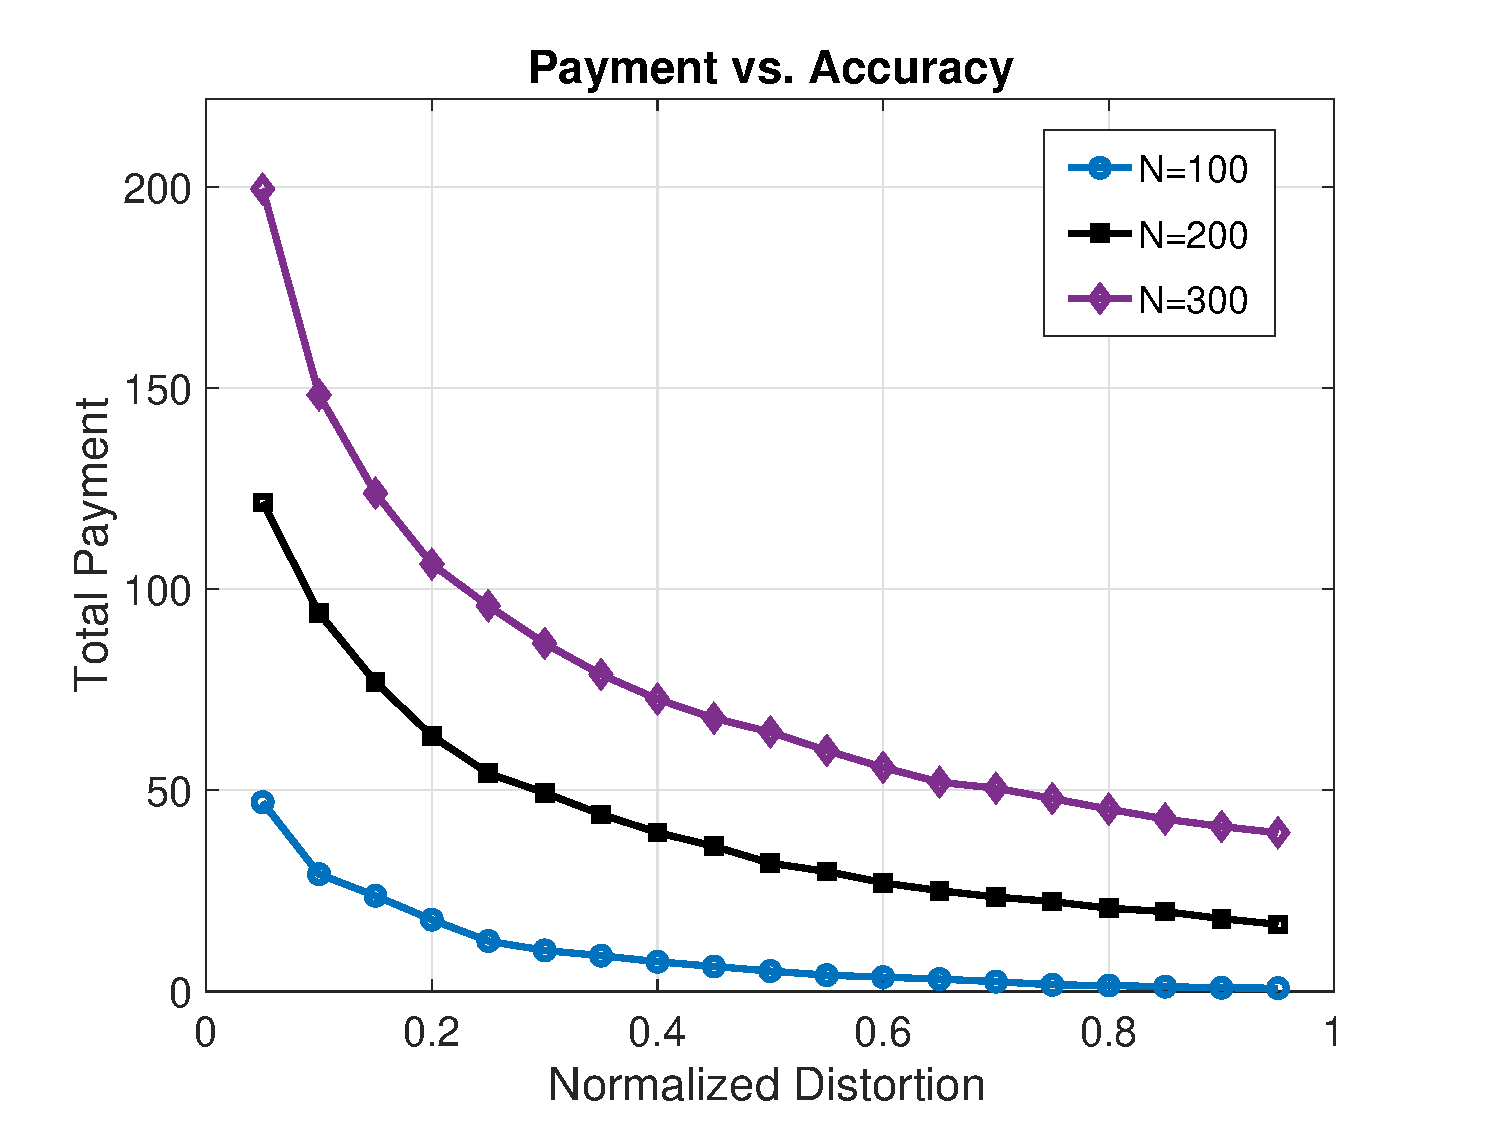
\includegraphics[scale=0.3]{./pic/payment_vs_accuracy5.eps}
%			%\caption{Payments under different accuracy requirements (privacy-passive case).}\label{fg:payment}
%			\caption{不同准确性约束下的平台支付(消极隐私保护情况)。}\label{fg:payment}
%		\end{minipage}
%		\hfill
%		\begin{minipage}[t]{0.48\textwidth}
%			\centering
%			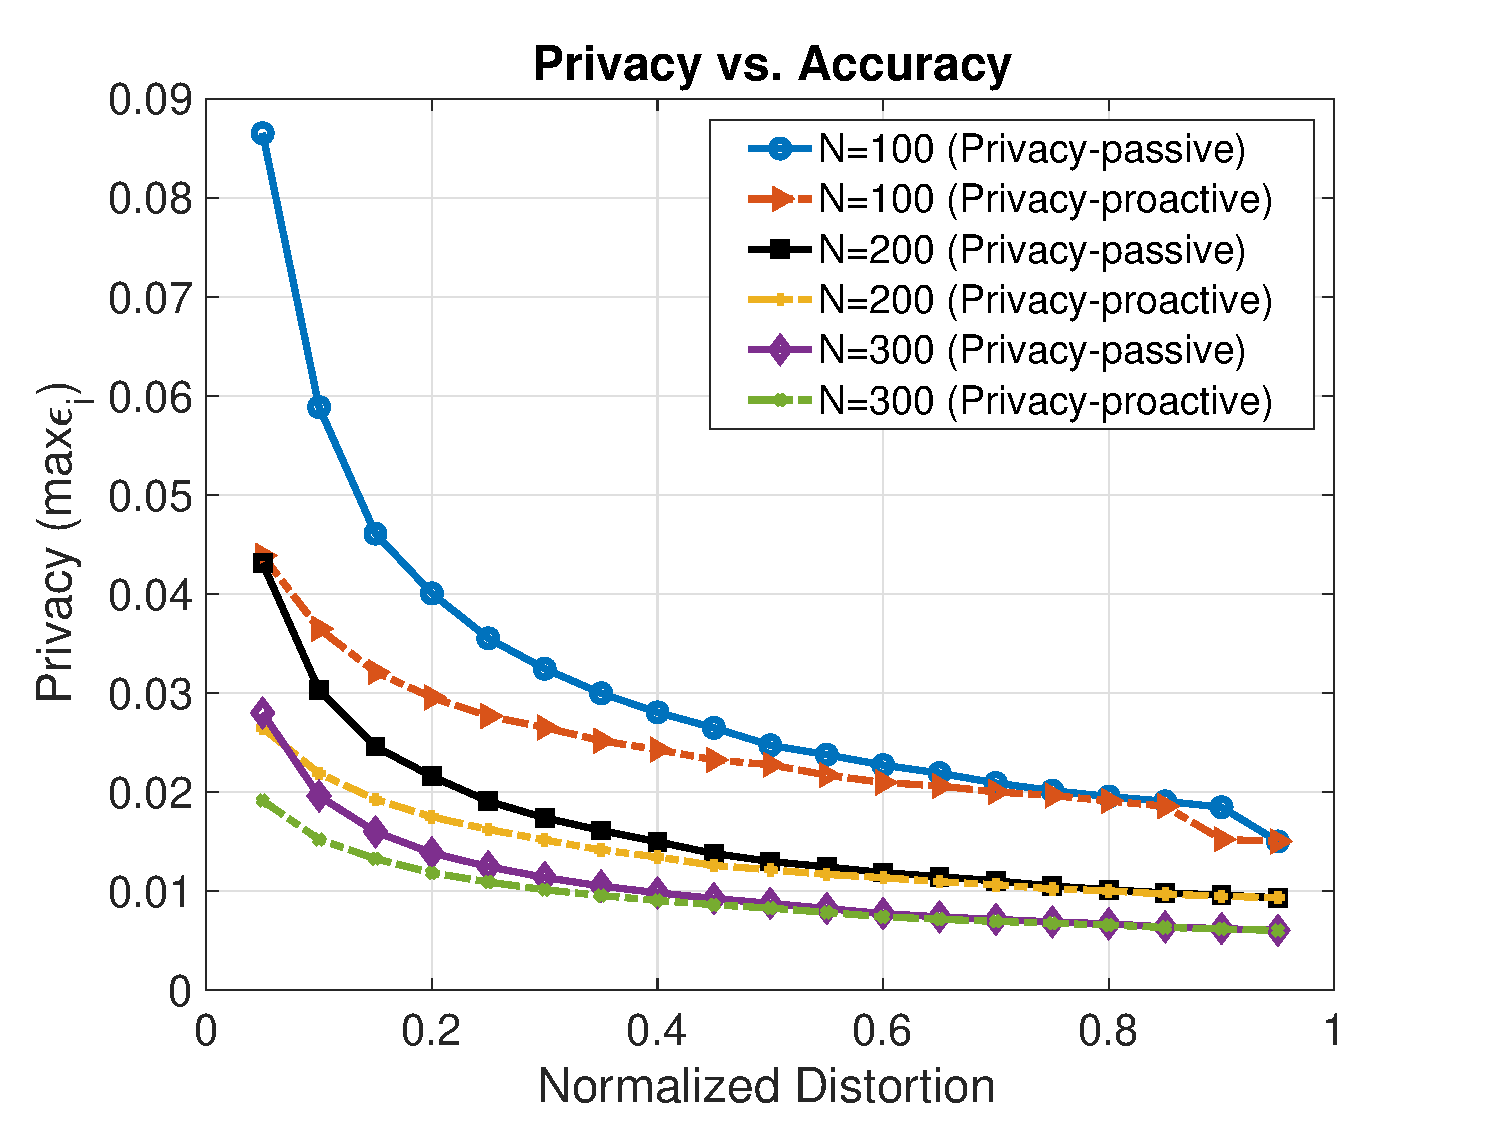
\includegraphics[scale=0.3]{./pic/privacy_vs_accuracy4.eps}
%			\caption{数据隐私与准确性之间的关系。}\label{fg:privacy}
%		\end{minipage}
%	\end{figure*}
	
	\begin{figure*}[!t]
%		\begin{minipage}[t]{0.48\textwidth}
			\centering
			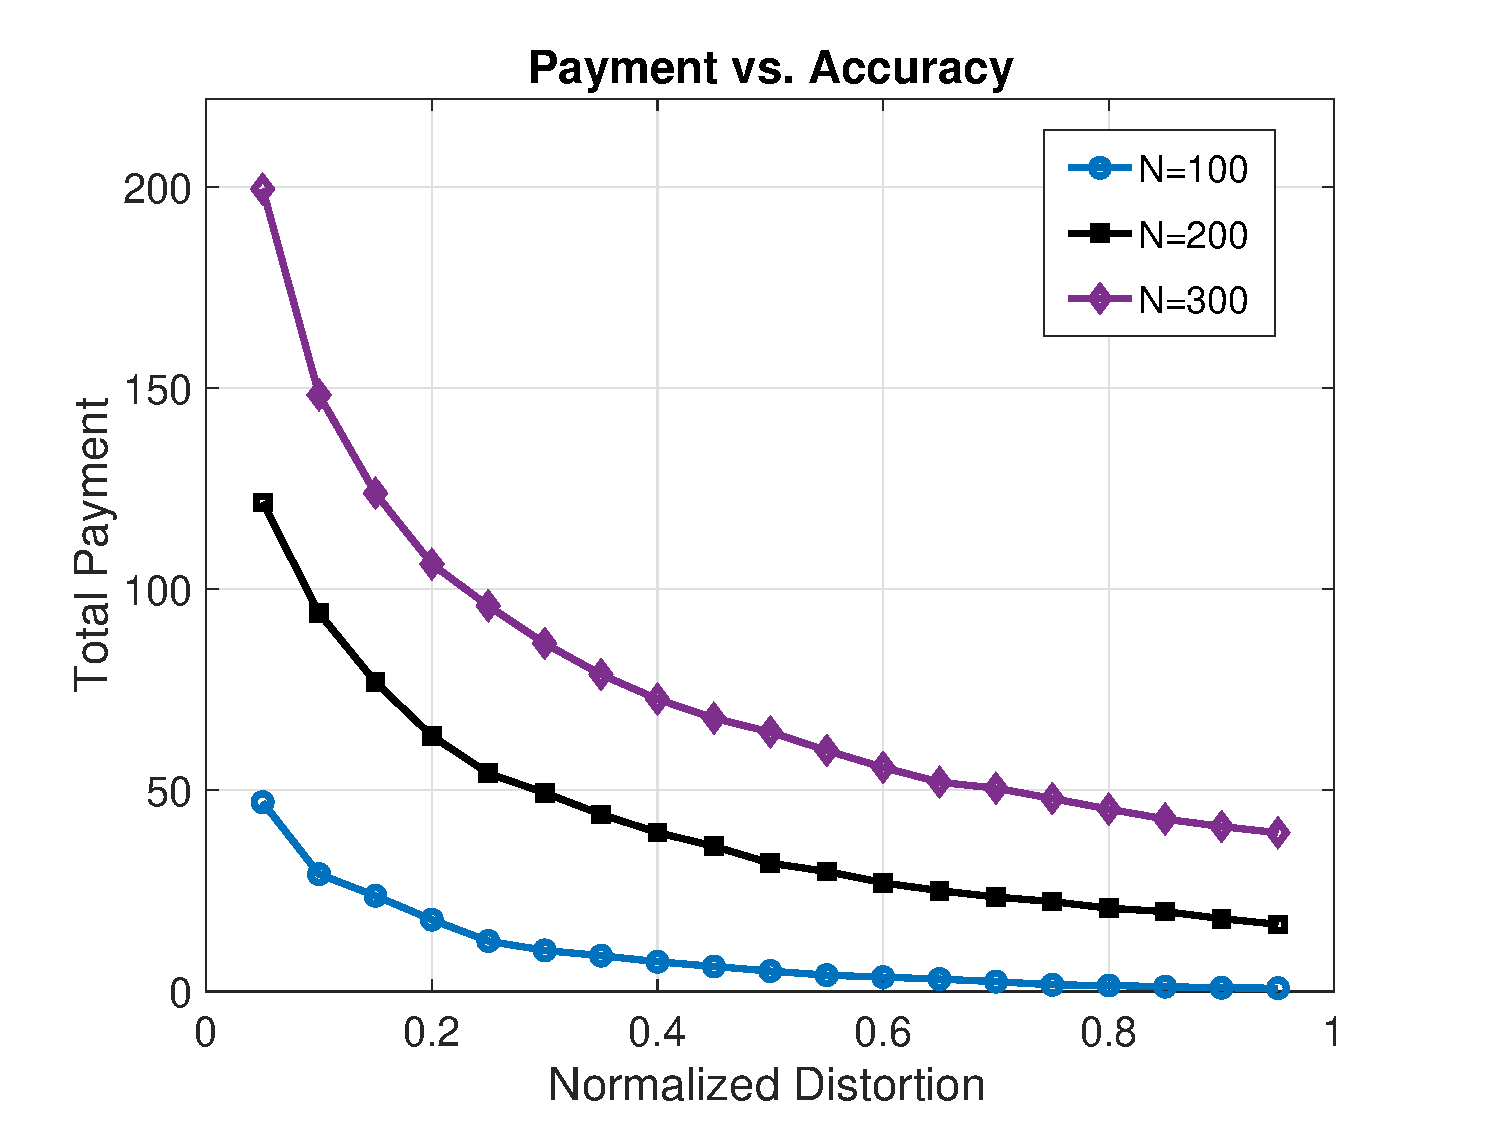
\includegraphics[scale=0.5]{./pic/payment_vs_accuracy5.eps}
			%\caption{Payments under different accuracy requirements (privacy-passive case).}\label{fg:payment}
			\caption{不同准确性约束下的平台支付(消极隐私保护情况)}\label{fg:payment}
	\end{figure*}
%		\end{minipage}
%		\hfill
%		\begin{minipage}[t]{0.48\textwidth}
	\begin{figure*}[!t]
			\centering
			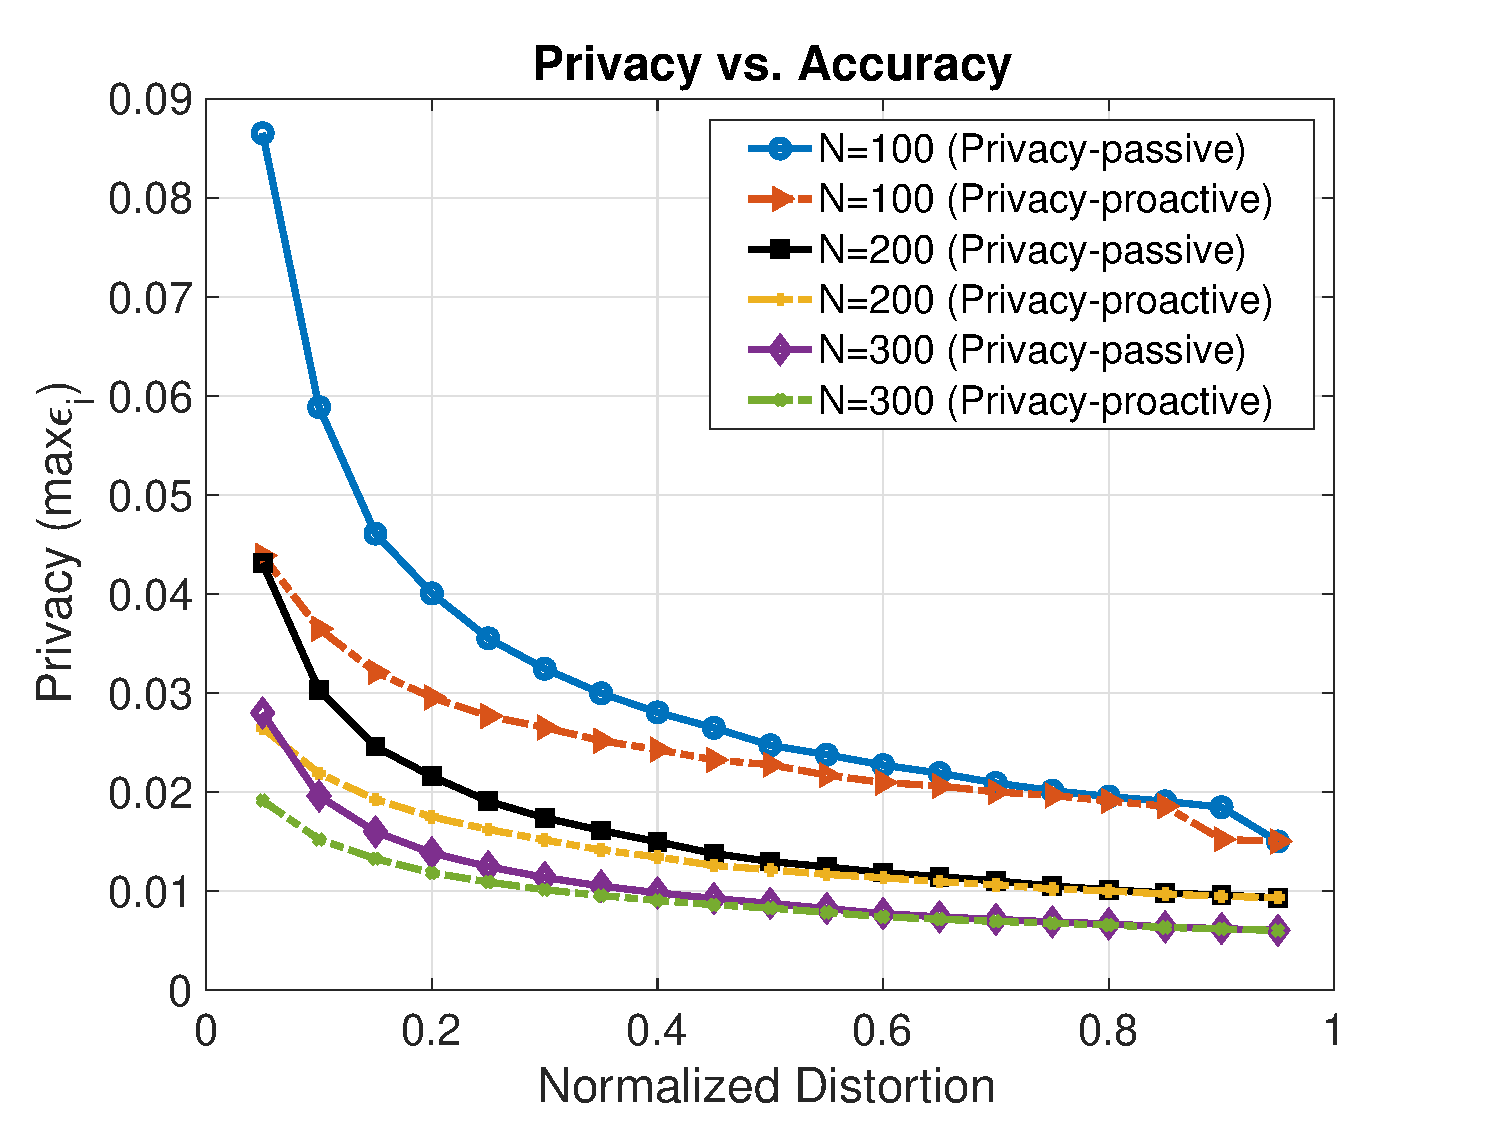
\includegraphics[scale=0.5]{./pic/privacy_vs_accuracy4.eps}
			\caption{数据隐私与准确性之间的关系}\label{fg:privacy}
%		\end{minipage}
	\end{figure*}	
	
	
	
	
	
%		\hfill
%		\begin{minipage}[t]{0.3\linewidth}
%			\centering
%			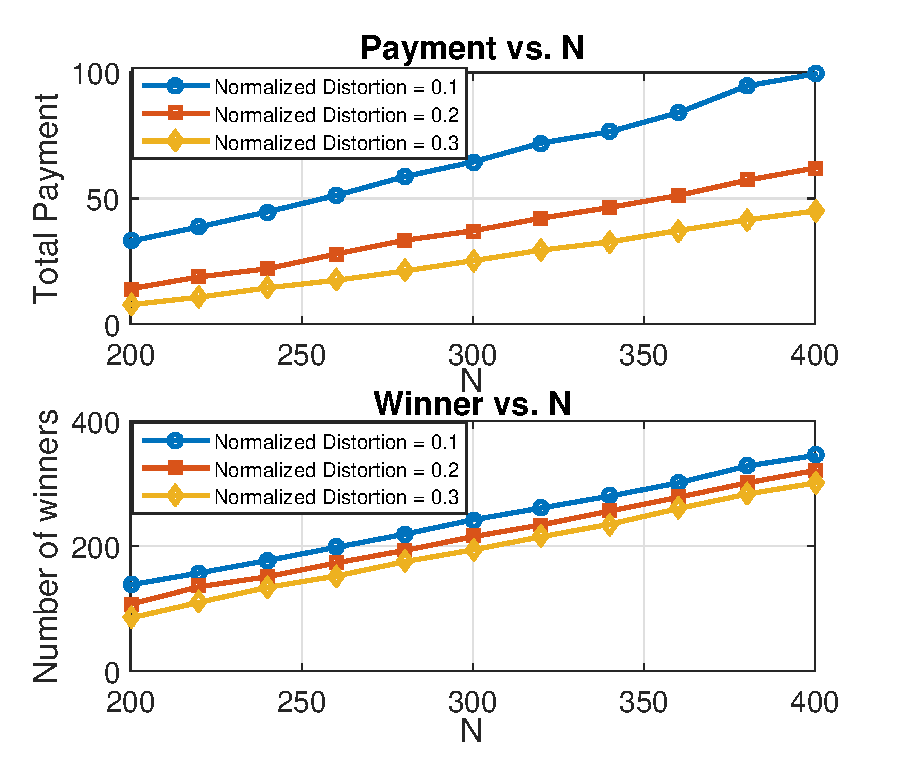
\includegraphics[scale=0.39]{./pic/externalities.eps}
%			\caption{Effect of externalities.}\label{fg:externalities}
%		\end{minipage}
		%\vspace{-0.5cm}
%		\vfill
%		\begin{minipage}[t]{0.48\textwidth}
%			\centering
%			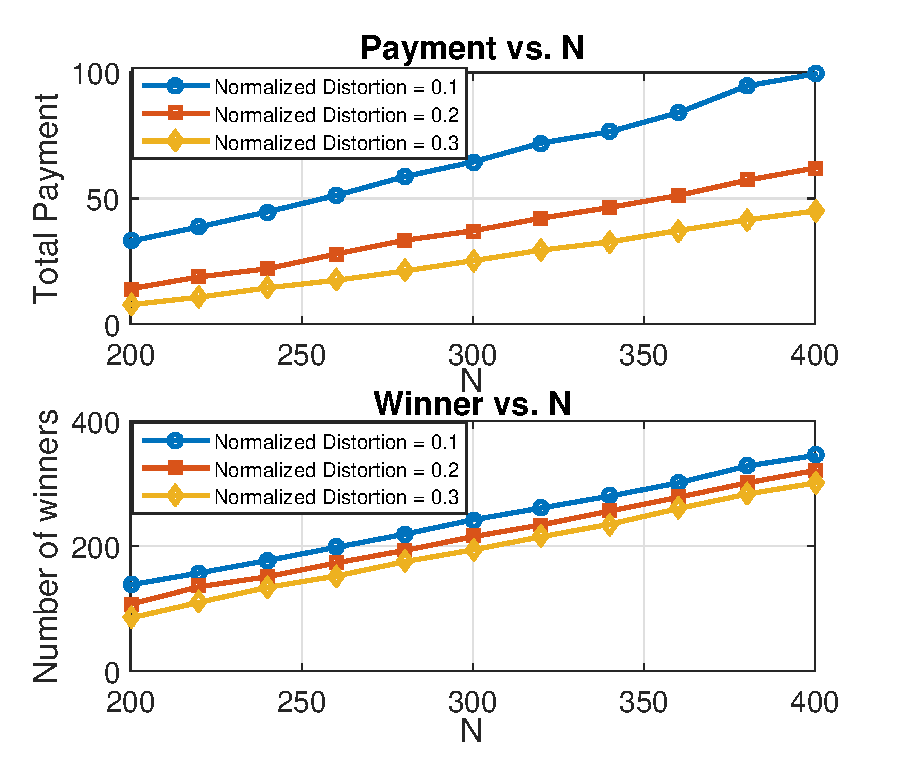
\includegraphics[scale=0.5]{./pic/externalities.eps}
%			\caption{Effect of externalities (privacy-passive case).}\label{fg:externalities1}
%		\end{minipage}
%	\begin{figure}
%		%\small
%		\subfigure[Privacy-passive case under different accuracy requirements.]{
%		\begin{minipage}[b]{0.45\textwidth}
%			\centering
%			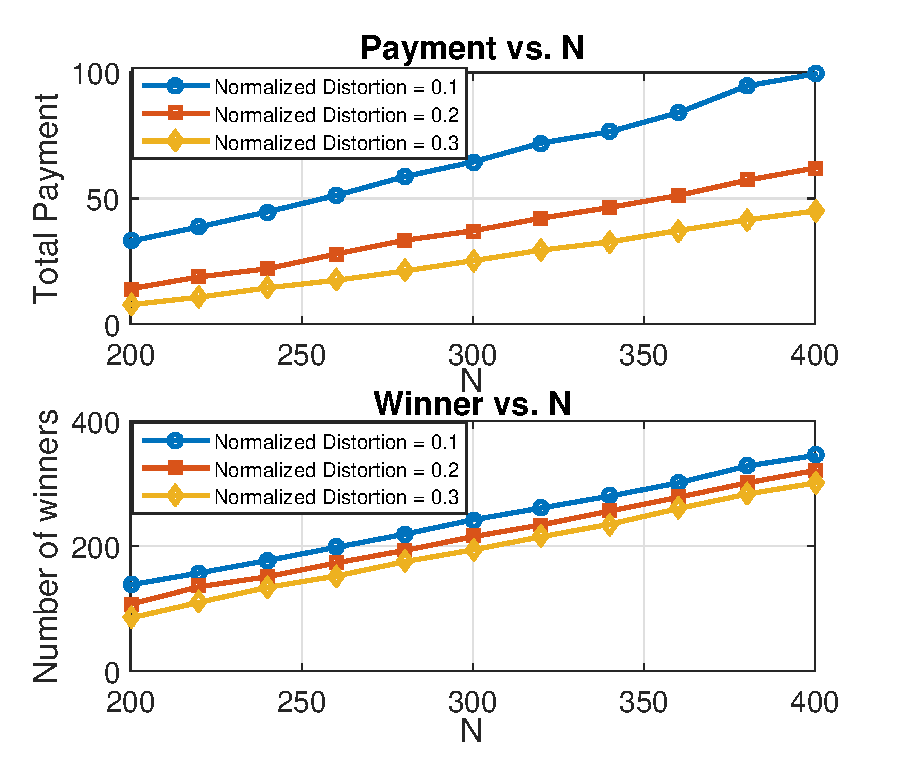
\includegraphics[scale=0.6]{./pic/externalities.eps}			
%		\end{minipage}}\label{fg:externalities1}
%		\subfigure[Comparison between privacy-passive case and privacy-proactive case (normalized distortion = 0.2).]{
%		\begin{minipage}[b]{0.45\textwidth}
%			\centering
%			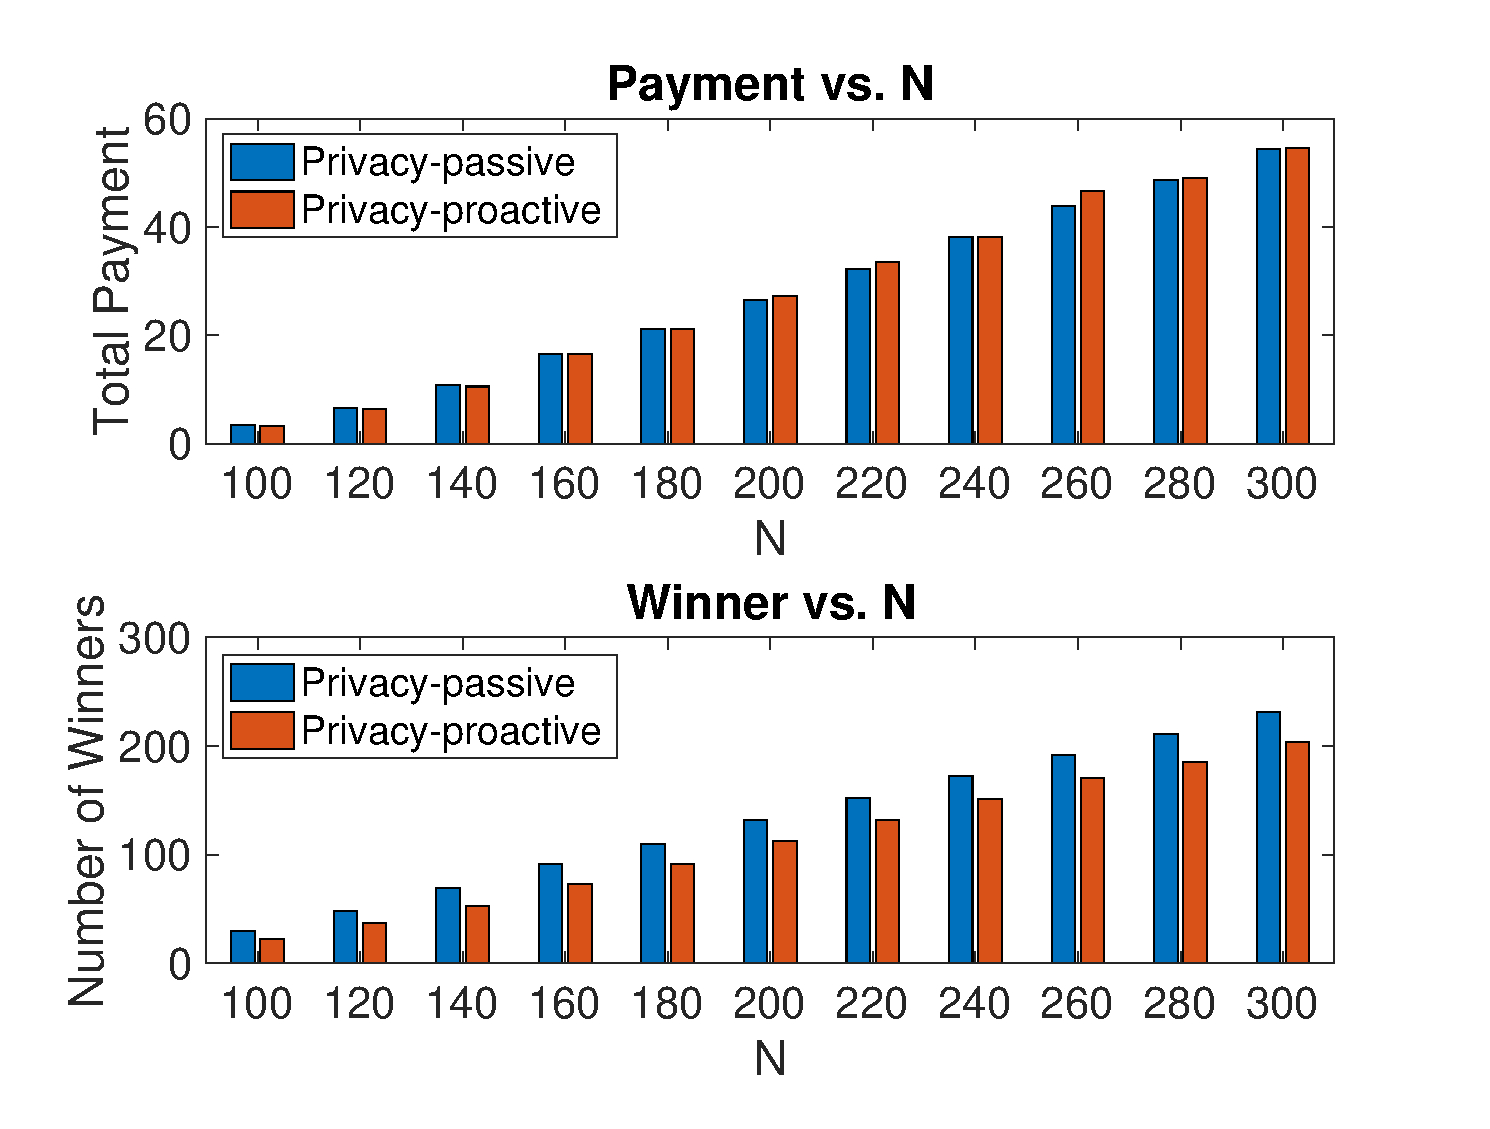
\includegraphics[scale=0.4]{./pic/externalities3.eps}
%		\end{minipage}}\label{fg:externalities2} %% label for second subfigure
%		\caption{Effect of externalities}
%		\label{fg:externalities}
%	\end{figure}
		
%	\begin{figure*}[!t]
%		\begin{minipage}[t]{0.48\textwidth}
%			\centering
%			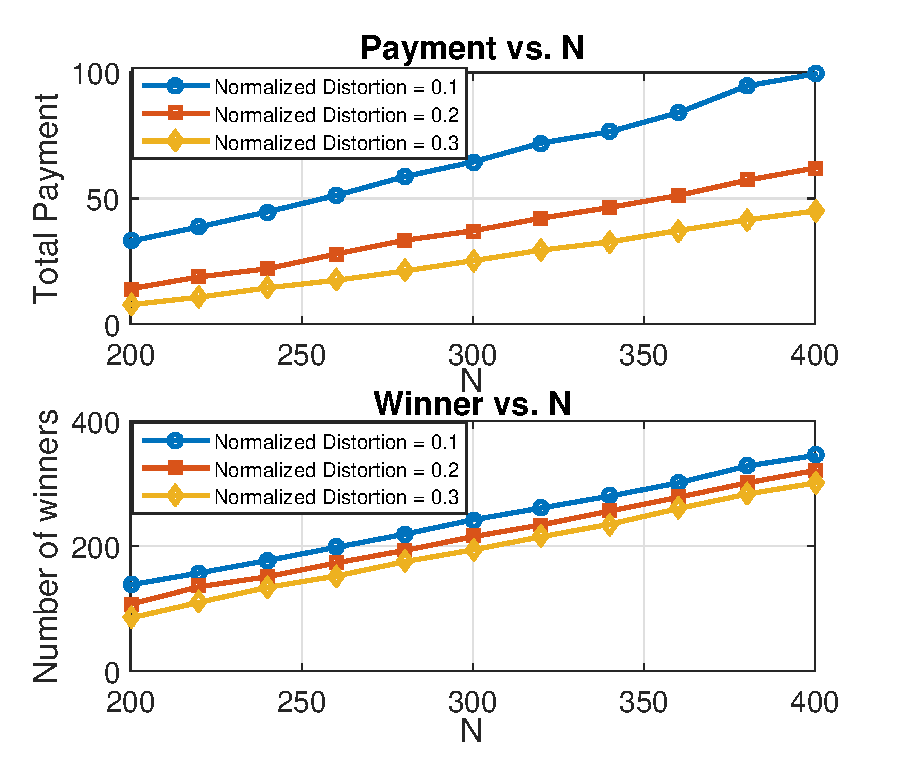
\includegraphics[scale=0.6]{./pic/externalities.eps}
%			\caption{不同准确性约束下用户总量的影响(消极隐私保护情况)。}\label{fg:externalities1}
%		\end{minipage}
%		\hfill
%		\begin{minipage}[t]{0.48\textwidth}
%			\centering
%			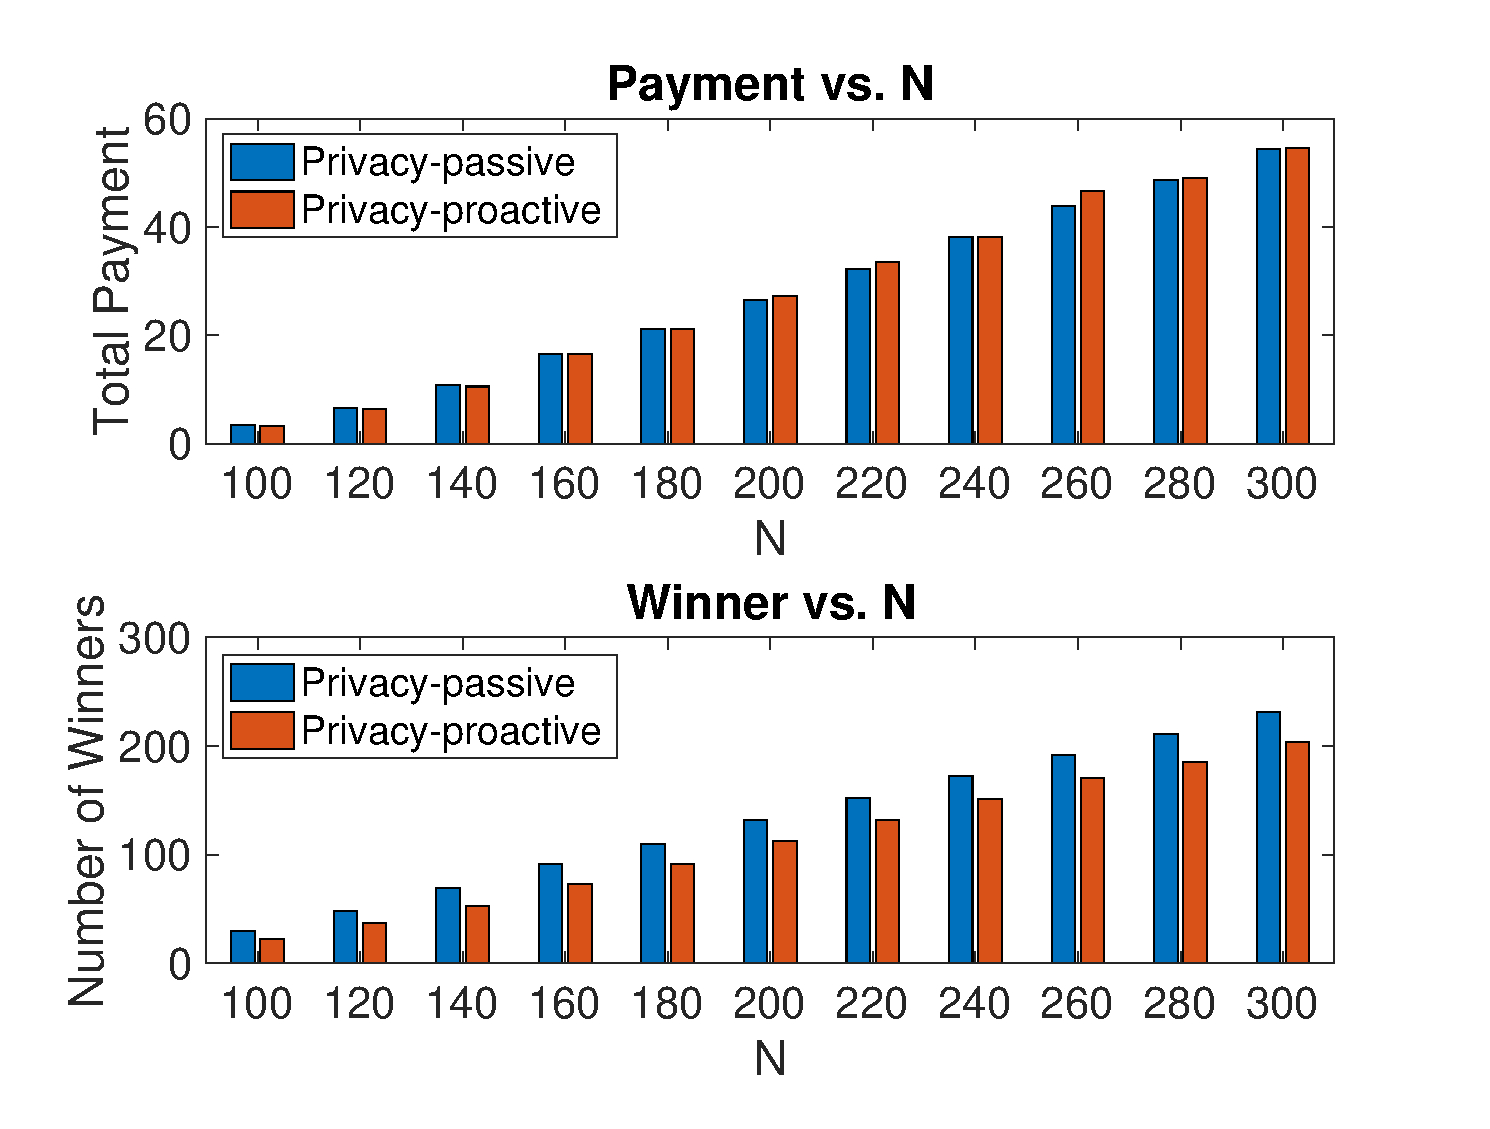
\includegraphics[scale=0.4]{./pic/externalities3.eps}
%			\caption{积极隐私保护与消极隐私保护之间的结果对比(归一化失真度要求 = 0.2)。}\label{fg:externalities2}
%		\end{minipage}
%		\caption{外部性影响}
%		\label{fg:externalities}
%	\end{figure*}		
	
	\begin{figure*}[!t]
%		\begin{minipage}[t]{0.48\textwidth}
			\centering
			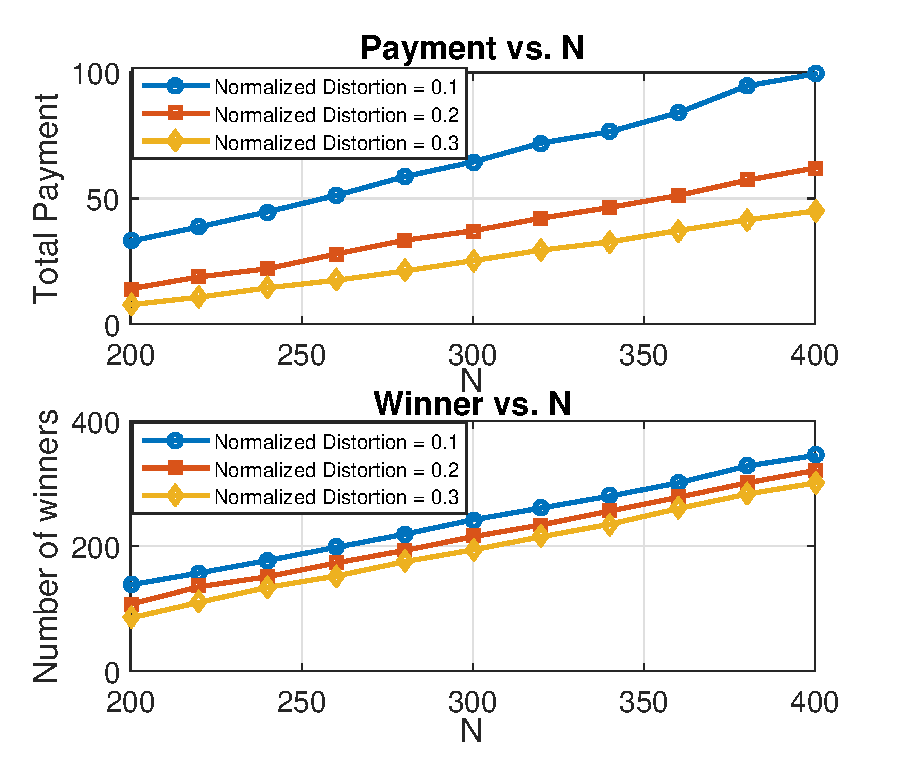
\includegraphics[scale=0.84]{./pic/externalities.eps}
			\caption{不同准确性约束下用户总量的影响(消极隐私保护情况)}\label{fg:externalities1}
%		\end{minipage}
%		\hfill
%		\begin{minipage}[t]{0.48\textwidth}
	\end{figure*}
	\begin{figure*}[!t]
			\centering
			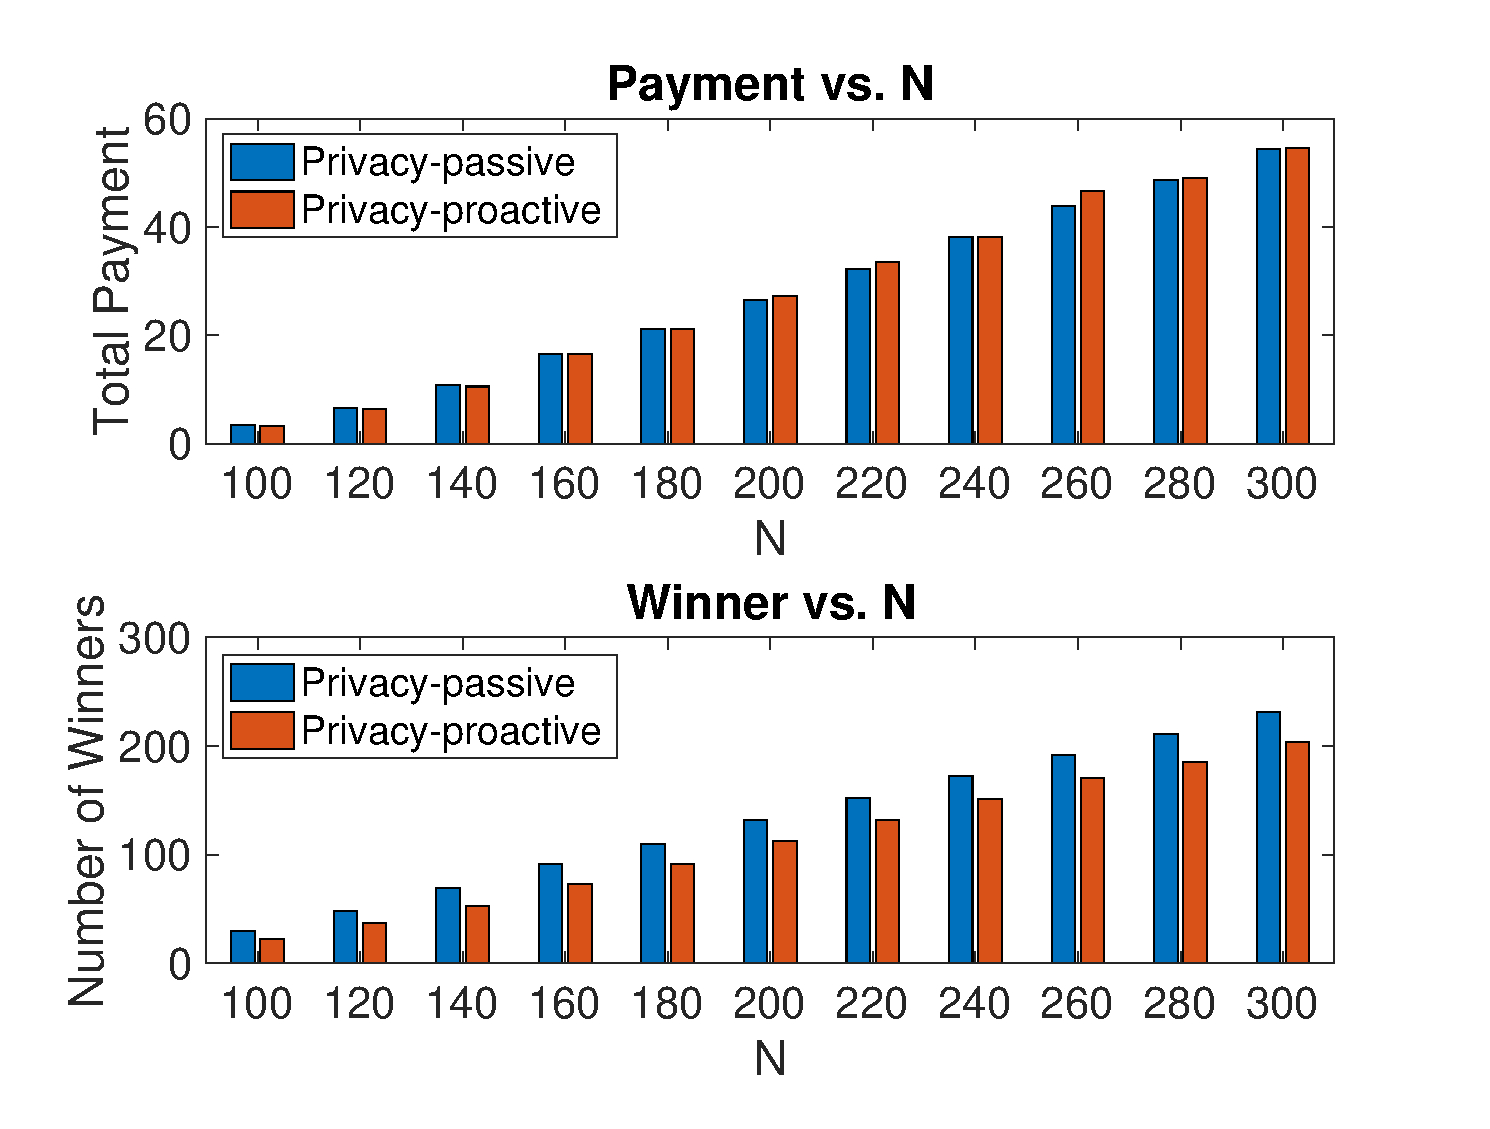
\includegraphics[scale=0.58]{./pic/externalities3.eps}
			\caption{积极隐私保护与消极隐私保护之间的结果对比(归一化失真度要求 = 0.2)}\label{fg:externalities2}
%		\end{minipage}
%		\caption{外部性影响}
%		\label{fg:externalities}
	\end{figure*}		
	
%		\centering
%		\subfloat[Privacy-passive case under different accuracy requirements.]{
%			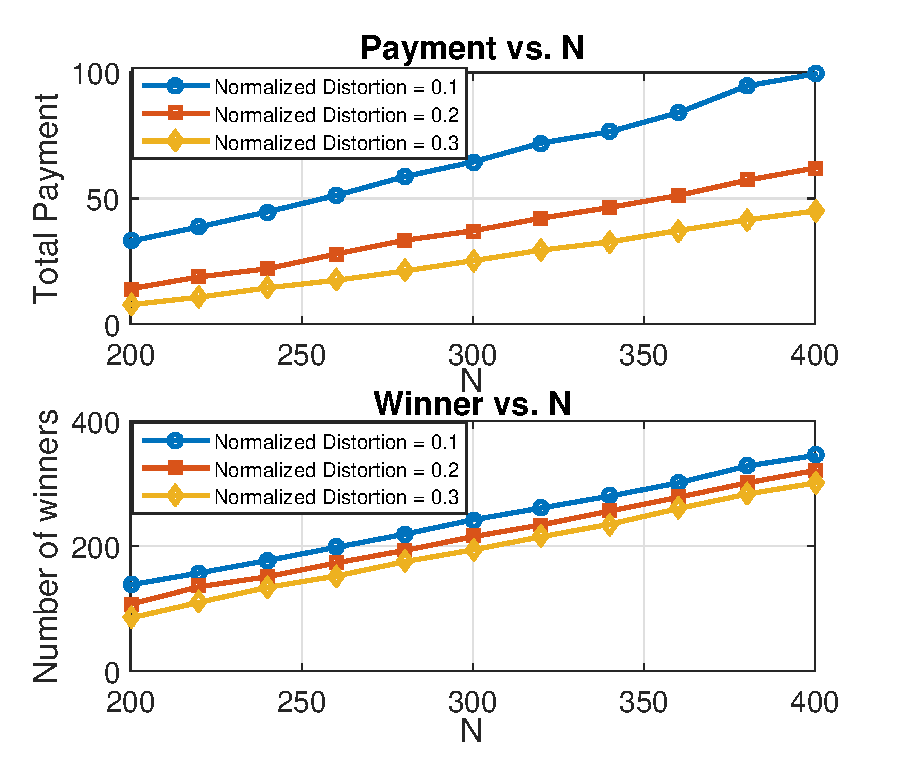
\includegraphics[scale=0.5]{./pic/externalities.eps}\label{fg:externalities1}}
%		%\hspace{0.45in}
%		\hfill
%		\centering
%		\subfloat[Comparison between privacy-passive case and privacy-proactive case (normalized distortion = 0.2).]{
%			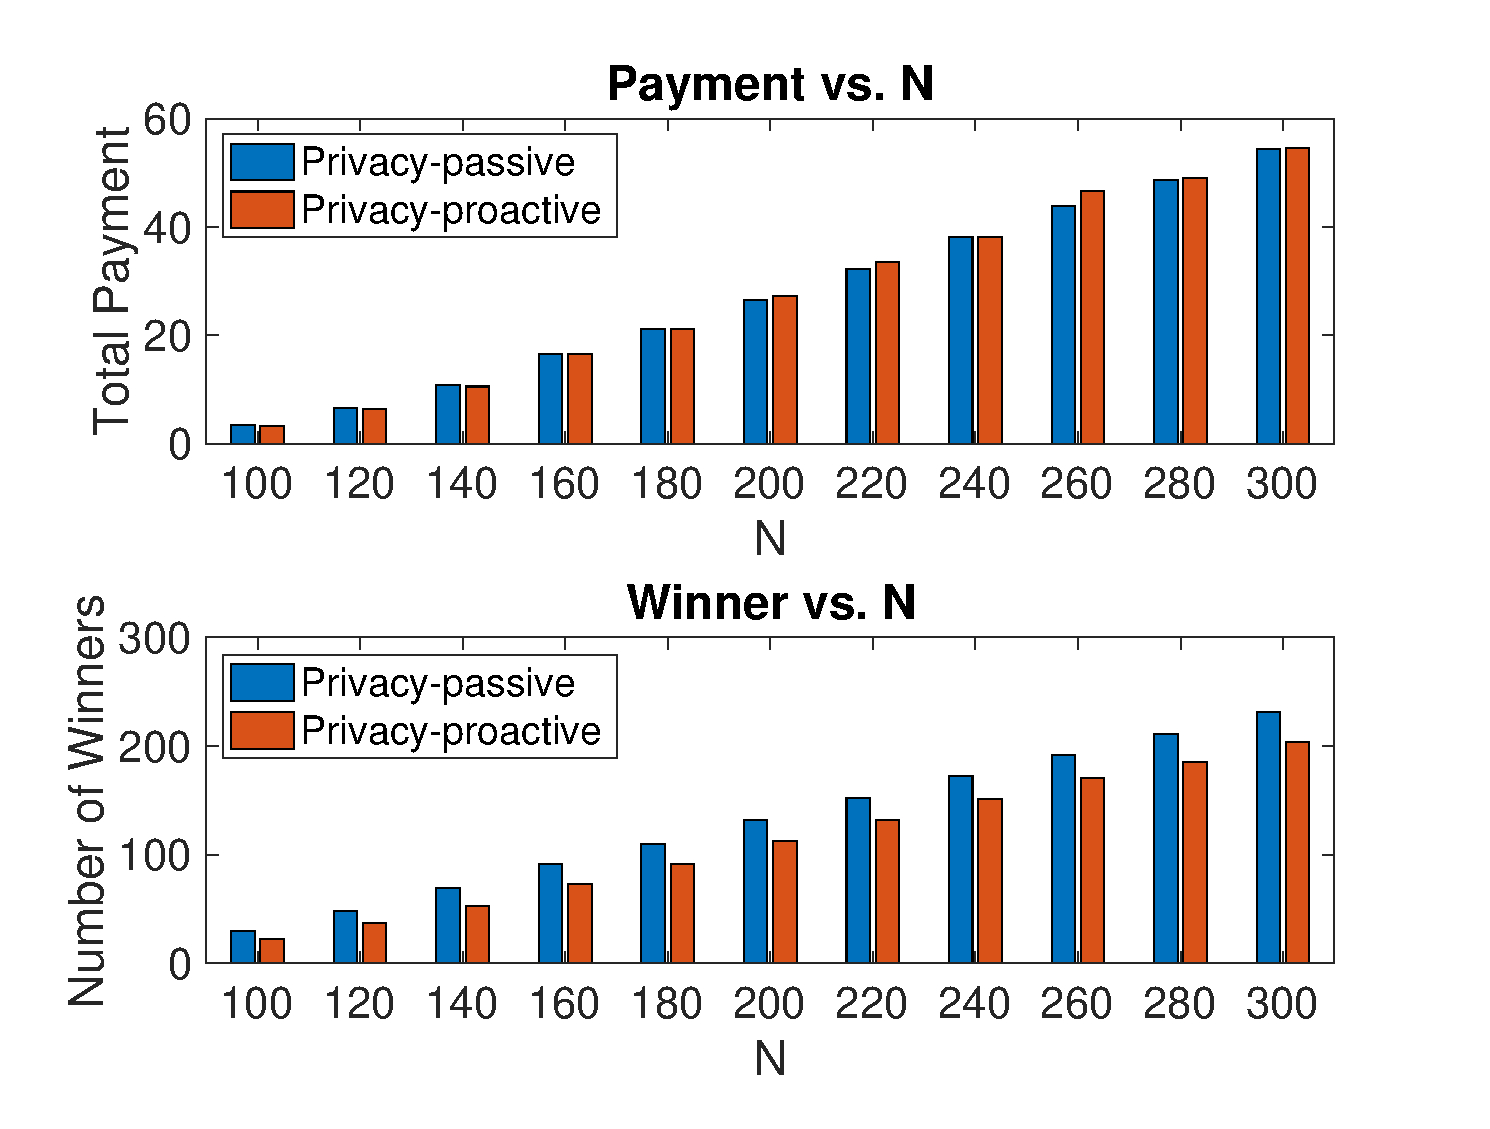
\includegraphics[scale=0.34]{./pic/externalities3.eps}\label{fg:externalities2}}
%		\hfill
%%		\begin{minipage}[t]{0.48\textwidth}
%%			\centering
%%			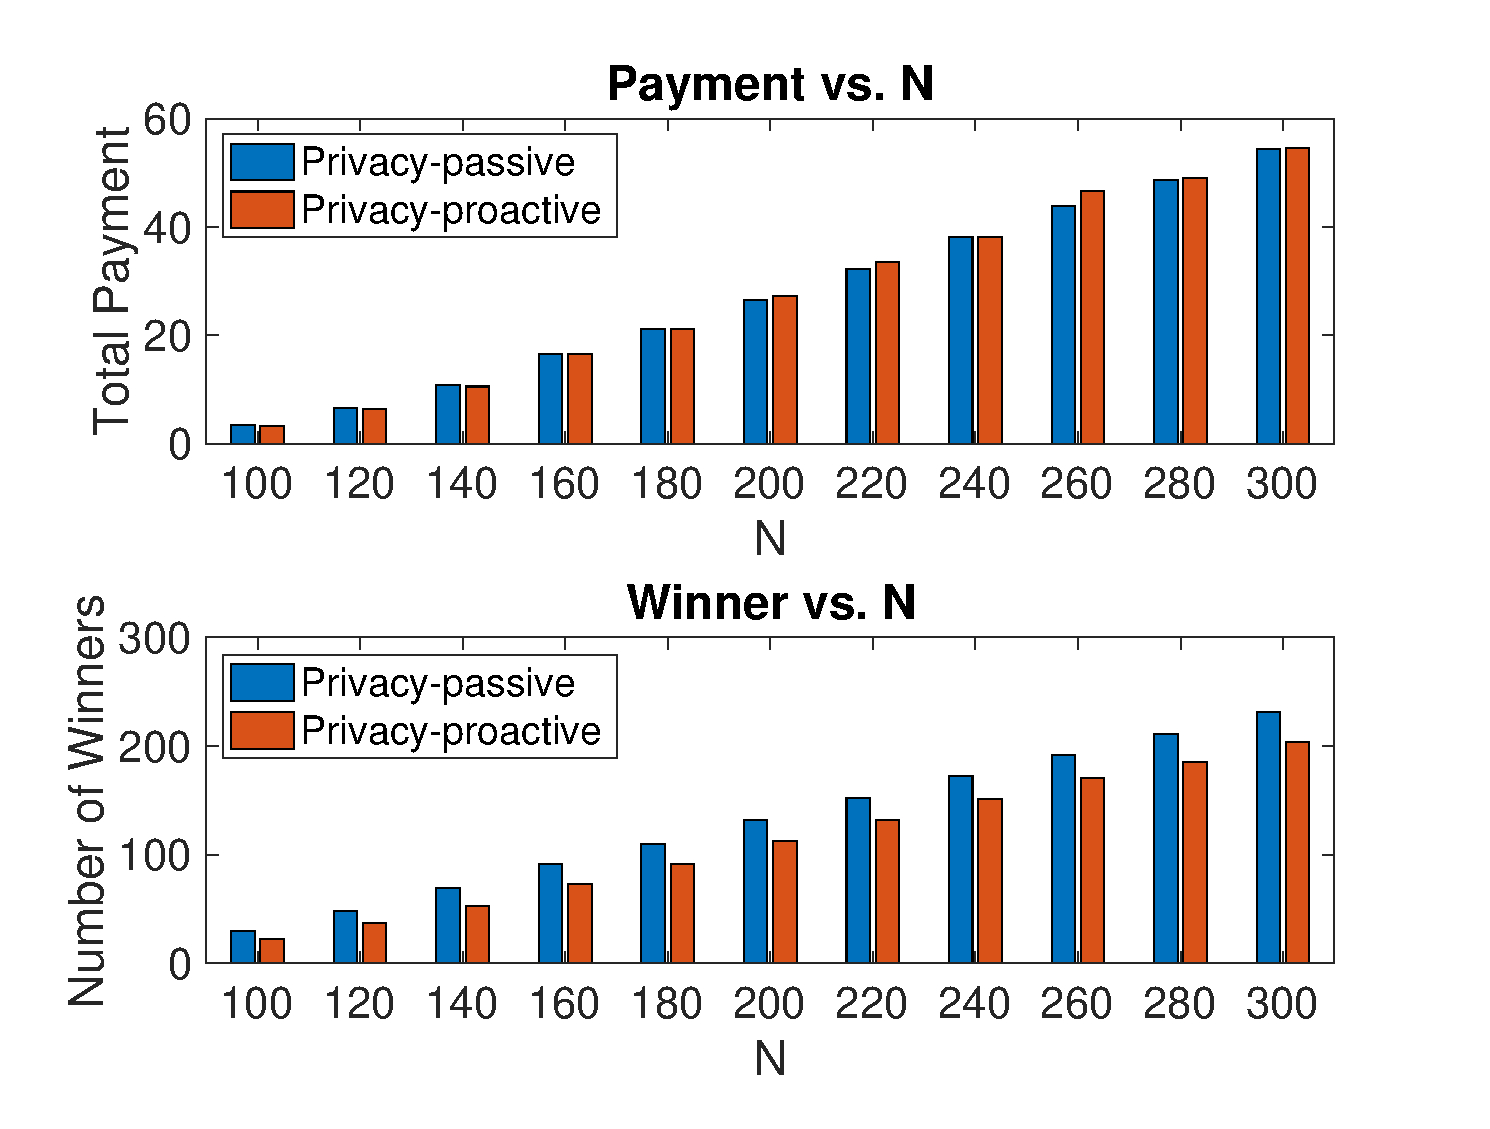
\includegraphics[scale=0.34]{./pic/externalities3.eps}
%%			\caption{Comparison between privacy-passive case and privacy-proactive case (normalized distortion = 0.2).}\label{fg:privacy}
%%		\end{minipage}
%		\caption{Effect of externalities}\label{fg:externalities}
		
		
		
%		\begin{minipage}[t]{0.3\linewidth}
%			\centering
%			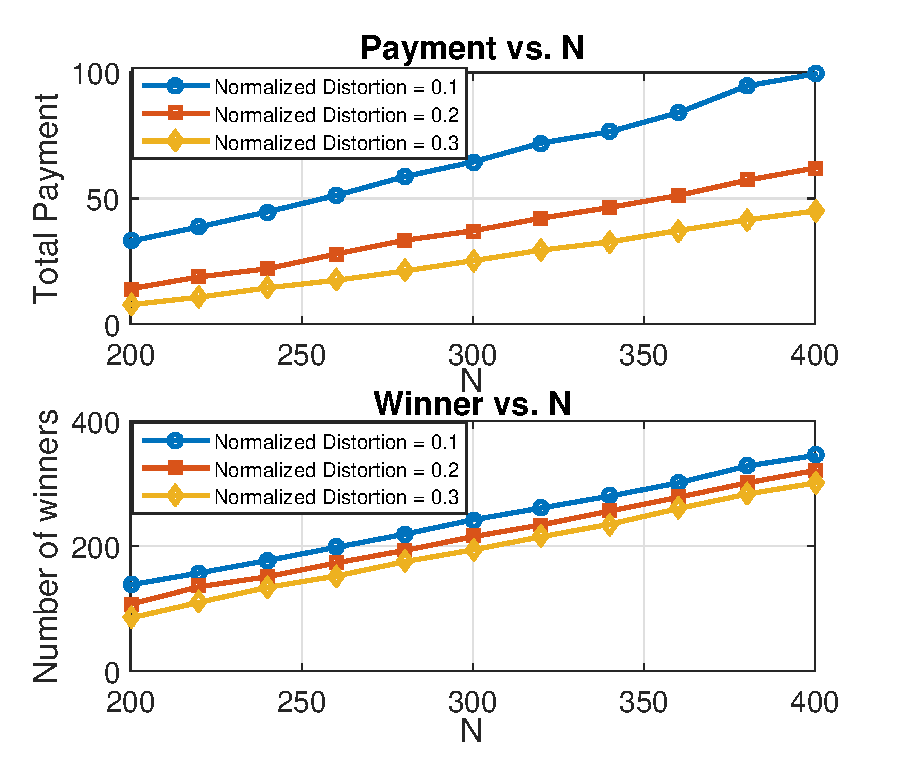
\includegraphics[scale=0.39]{./pic/externalities.eps}
%			\caption{Effect of externalities.}\label{fg:externalities}
%		\end{minipage}
%		\hfill
%		\begin{minipage}[t]{0.3\linewidth}
%			\centering
%			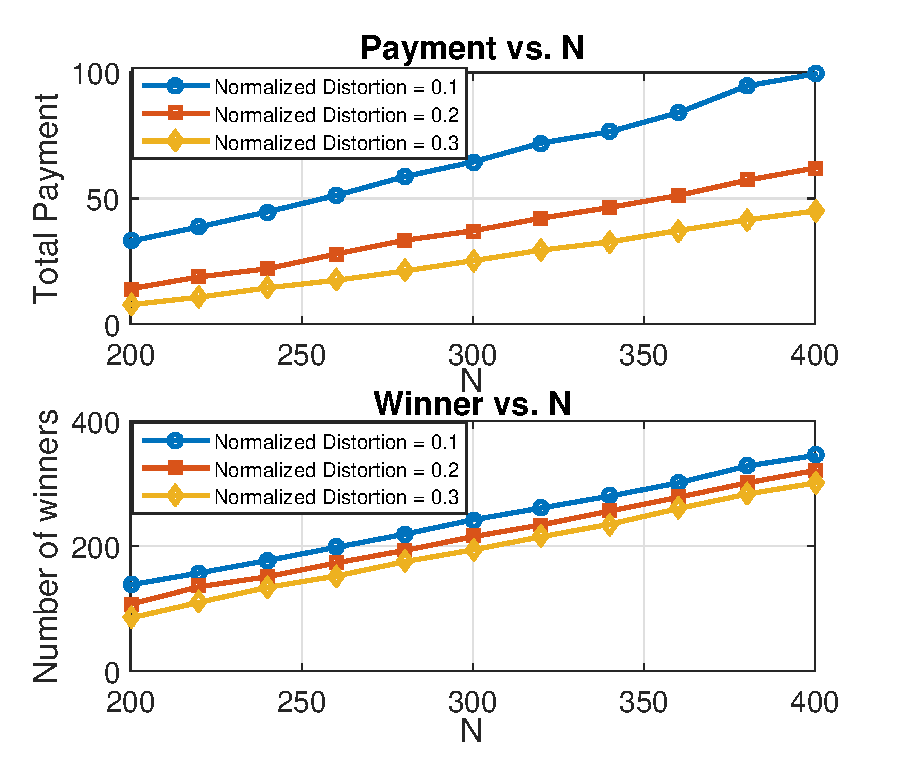
\includegraphics[scale=0.39]{./pic/externalities.eps}
%			\caption{Effect of externalities.}\label{fg:externalities}
%		\end{minipage}
	
%	\end{figure*}

\section{性能评估}\label{sec:pe}

\subsection{仿真设置}\label{sec:setup}
	在仿真中,我们随机生成用户的竞标价。具体的,我们从区间$[1, 20]$均匀地生成用户$i$的单位隐私成本$v_i$;对于积极隐私保护场景,我们从区间$[0.01, 0.2]$均匀地生成用户$i$的隐私保护级别固有要求$E_i$。我们从区间$[1,10]$均匀地随机生成每一个用户的权值,然后进行归一化处理。实验中的用户总数$N$的变化范围为100到300。失真度通过预设的最大失真度$\Delta_{\max}$进行归一化处理,保证$W$在不同失真度情况下总为正值。我们使用优化求解器CPLEX\cite{CPLEX}的二等分算法求解问题(\ref{eq:problem2})和问题(\ref{eq:problem1b})的最优解。由于据我们所知, 现有的群智感知激励机制研究工作尚未有考虑系统网络外部性的特征,因此在这里我们仅对DPDA算法和EDPDA算法进行评估实验。
	%In our simulation, we generate workers' bids at random. Specifically, the unit privacy costs are generated uniformly from the interval $[1, 20]$ and the data privacy level requirements are generated uniformly from the interval $[0.01, 0.2]$. The weights of workers are first generated uniformly at random from the interval $[1,10]$ and then normalized. The number of workers $N$ varies from 100 to 300. The distortion is normalized by some largest distortion $\Delta_{\max}$ such that $W$ is always positive under different distortions. The optimal solutions to the problem (\ref{eq:problem2}) and (\ref{eq:problem1b}) are calculated based on the bisection algorithm using the CPLEX optimization solver \cite{CPLEX}. To the best of our knowledge, as there are no auction mechanisms for mobile crowdsensing allowing workers to report noisy data while considering the externalities, we examine only the performance of the DPDA algorithm and the EDPDA algorithm we proposed in this paper.
	
	\vspace{-0.2cm}
	\subsection{结果和讨论}
	
	%\noindent{\textbf{Payment versus Accuracy.}}
	\noindent{\textbf{奖励 vs. 准确性}}
	在图\ref{fg:payment}中,我们展现了平台总支付在不同结果准确性约束下的变化趋势。我们观察到,随着准确性约束放宽(归一化失真度要求变大),平台总支付会单调降低。其背后原因是$W$会随着$\Delta$数值的增加而减少,即准确性要求放宽后平台不需要在“购买”较准确的用户隐私数据上产生过多成本。同时,我们发现对于相同水平的失真度要求,平台的总支付额随着用户总数的增加而增加。这是由于对于相同水平的失真,$W$随着用户数量的增加而增加(\ref{eq:problem2}),使得平台必须征召更多的用户,从而导致总付款额的增加。
	%In Fig. \ref{fg:payment}, we illustrate the payments under different accuracy requirements with different total number of privacy-passive workers. We observe that as the distortion level increases, the total payments decrease, simply because $W$ decreases as $\Delta$ increases, i.e., the platform does not need to purchase much privacy from workers. Meanwhile, for the same level of distortion, the total payments increase with the number of workers, because $W$ increases with the number of workers for the same level of distortion based on (\ref{eq:problem2}), which requires the platform to select more workers and thereby the total payments increase. 
	
	%\begin{figure}[h!]
	%	\centering
	%	\includegraphics[scale=0.4]{./pic/payment_vs_accuracy1.eps}
	%	\caption{Payments under different accuracy requirements with different total number of workers.}\label{fg:payment}
	%\end{figure}
	
	\noindent{\textbf{隐私 vs. 准确性}}
	在图\ref{fg:privacy}中,我们阐明了数据隐私保护级别与结果准确性约束之间的关系。我们使用所有参与用户中最低的隐私保护级别(即$\epsilon=\max_{i\in\mathcal{S}}\epsilon_i$)来表示某一准确性约束(失真度要求)的系统隐私保护级别。正如我们所预期的,随着准确性约束放宽,数据隐私保护级别会有所升高(即$\epsilon$越小,隐私保护级别越高),与节\ref{sec:pvsa}中的分析相符合。实验结果同时清除地表明积极隐私保护场景下的用户普遍会比消极隐私保护场景下的用户得到更高的隐私保护级别,而这正是由于积极隐私保护场景下的用户会对其隐私保护级别有固有的要求。
	%In Fig. \ref{fg:privacy}, we illustrate the relationship between the data privacy and the accuracy. As the privacy of each worker is different, we use the maximum of all the workers' $\epsilon_i$  ($\epsilon=\max_{i\in\mathcal{S}}\epsilon_i$) to denote the privacy protection level at the given distortion level. As expected, as the distortion level increases,  the data privacy level increases (the smaller $\epsilon$, the higher the privacy protection level), which agrees with our analysis in Section \ref{sec:pvsa}. The results clearly show that privacy-proactive workers in general experience higher privacy level than the privacy-passive workers, which agrees with our expectation since privacy-proactive workers have imposed customized privacy level requirement once enter into the crowdsensing system. 
	
	%\begin{figure}[h!]
	%	\centering
	%	\includegraphics[scale=0.4]{./pic/privacy_vs_accuracy2.eps}
	%	\caption{Relationship between data privacy and the accuracy.}\label{fg:privacy}
	%\end{figure}
	
	\noindent{\textbf{单重负网络外部性}}
	在图\ref{fg:externalities1}和图\ref{fg:externalities2}中,我们阐明了单重负网络外部性的影响。如同节\ref{sec:formulation}中所讨论的,每个用户的数据隐私保护级别取决于其他用户的参与。当参与用户的数量改变时,用户们的隐私保护级别也相应发生变化。当用户数量增加时,平台需要征召的用户数量也随即增加以维持相同的结果准确性。因此,我们可以从实验结果中观察到当用户总数增加时,平台的总支付和参与的用户数量都有相应的增加。图\ref{fg:externalities1}则清除地说明了准确性要求越低(失真度水平越高),平台总支付和参与的用户数量约少。
	%Fig. \ref{fg:externalities} illustrates the effect of externalities. As discussed in Section \ref{sec:formulation}, the data privacy level of each worker depends on other workers' participations, and when the  number of workers changes, it would change workers' privacy levels. As the number of workers increases, the platform needs to hire more workers to maintain the same distortion level. Therefore, we can observe that the increase of total payments and the number of winners as the worker set enlarges. Fig. \ref{fg:externalities1} clearly shows that the higher the distortion level, the lower the total payment and the less the number of winners. 
	在图\ref{fg:externalities2}中,我们进行了隐私消极保护场景和因司机及保护场景的对比。可以看到,在给定归一化失真度和用户集大小的情况下,两种场景下平台所需支付的总付款额几乎相同。这是由于积极隐私保护场景下参数$W$并不受用户$i\in\N$的固有隐私级别要求$g_i$的影响。此外,我们观察到,积极隐私保护场景下的拍卖获胜者人数通常少于消极隐私保护场景下的获胜者人数。这是因为对隐私保护级别的固有要求使少数用户失去了参与感知任务的条件,直接导致了用户人数的减少。因而在单重负外部性的影响下,获胜者的数量减少了。
	%In Fig. \ref{fg:externalities2}, we show the comparison results of the privacy-passive case and privacy-proactive case. We can see that almost the same total payment has to be consumed in the two cases given a fixed normalization distortion with a fixed size of worker set, as $W$ is not influenced by the imposed privacy level requirement $g_i$ of each worker $i\in\N$. Moreover, we observe that the number of winners in the privacy-proactive case is in general less than the number of winners in the privacy-passive case. This is because the additional requirement on privacy level renders a few workers unqualified for being evolved into the private crowdsensing, which leads to the shrink of worker set. Under the effect of externality, the number of winners decreases.

	
	%\begin{figure}[h!]
	%	\centering
	%	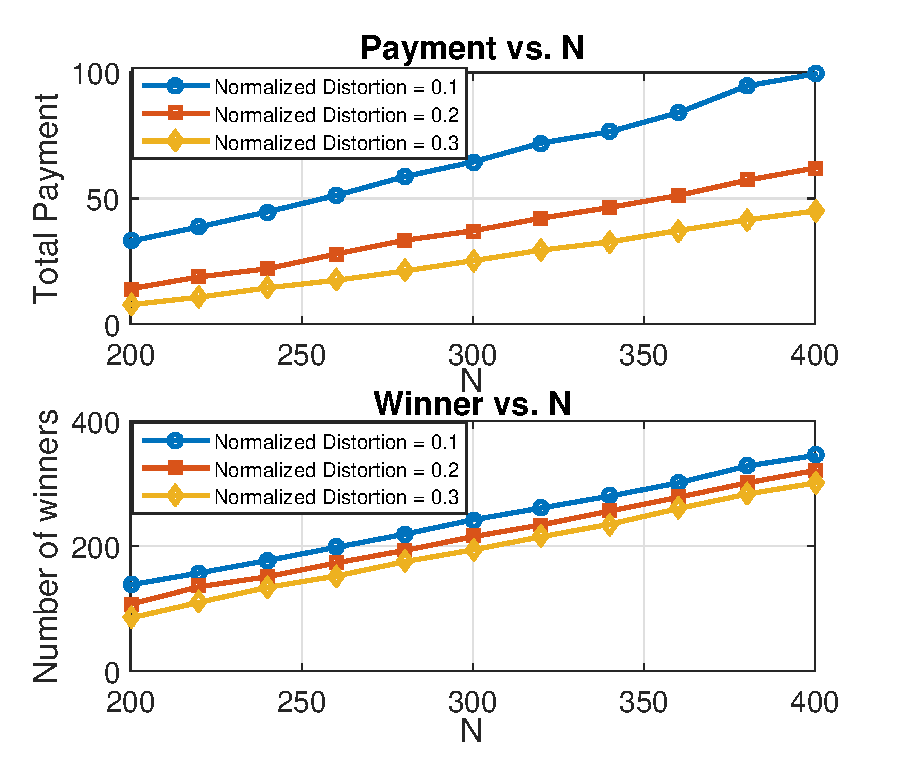
\includegraphics[scale=0.4]{./pic/externalities.eps}
	%	\caption{Effect of externalities.}\label{fg:externalities}
	%\end{figure}
	
	
	\noindent{\textbf{算法近似度}}
	在表\ref{tab:optimality}中,我们通过分别比较DPDA算法和EDPDA算法输出结果与相应最优值的差异来说明两个算法的性能。对于每个$N$的取值,我们运行100次实验,并且在每个实验中,我们都会随机生成节\ref{sec:setup}中提到的参数。
	%In Table \ref{tab:optimality}, we illustrate the performance of the proposed DPDA algorithm and EDPDA algorithm respectively by comparing their output total payment with the optimal ones. For each $N$, we run 100 experiments and in each experiment, we randomly generate the parameters as mentioned in Section \ref{sec:setup}. 
	在不同的实验设置下,我们观察到两种算法得到的总付款都非常接近最优值,两个算法的最大近似比约为2。
	%Under different settings, we observe that the total payments generated by these two algorithms are very close to the optimal one and the maximal approximation ratio for each case is around 2. 
	相比之下,DPDA算法的近似率优于EDPDA。这是因为在积极隐私保护的场景下,平台除了要考虑成本最小化的目标外,还须考虑用户的固有隐私保护级别要求。
	%EDP​​DA算法的拍卖获胜者选择过程通过先筛选出满足隐私保护级别要求的工人,然后选择优化付款的获胜者,而不是在选择获胜者时共同考虑这两个因素,从而将这两个因素解耦。
	%By comparison, DPDA algorithm outperforms EDPDA in terms of the approximation ratio. This is because that in the privacy-proactive scenario, the platform has to take into account workers' privacy level requirements in addition to the objective of payment minimization. And the winner determination procedure of EDPDA algorithm decouples the two factors by first filtering out workers whose privacy level requirements are satisfied, then selecting out winners that optimize the payment, instead of jointly considering both two factors while choosing the winners.
	
%	\begin{table}[h!]
%			\vspace{-0.3cm}
%		\caption{Approximation ratio of the DPDA algorithm, where we choose the normalized distortion equal to 0.2.}
%		\vspace{-0.2cm}
%		\label{tab:optimality}
%		\centering \tabcolsep 5pt
%		\begin{tabular}{|c|c|c|c|}
%			\hline
%			Number of workers $N$  & 200 & 300 & 400 \\
%			\hline
%			Average approximation ratio   & 1.88 &1.85& 1.85\\
%			\hline
%			Minimal approximation ratio   & 1.71 &1.69& 1.70\\
%			\hline
%			Maximal approximation ratio   &  2.15    & 2.07   & 1.99      \\
%			\hline
%		\end{tabular}
%
%	\end{table}

	\begin{table}[h!]
%			\vspace{-0.3cm}
		\caption{DPDA和EDPDA算法的近似率(归一化失真度要求 = 0.2).}\label{tab:optimality}
		%\vspace{-0.3cm}
		
		\centering \tabcolsep 5pt
%		\subfloat[DPDA Algorithm]{
		\subfigure[DPDA算法]{
		\begin{tabular}{|c|c|c|c|}
			\hline
			用户总数 $N$  & 100 & 200 & 300 \\
			\hline
			平均近似率   & 1.88 &1.85& 1.85\\
			\hline
			最小近似率   & 1.45 &1.68& 1.70\\
			\hline
			最大近似率   &  2.21    & 2.23   & 2.08 \\
			\hline
		\end{tabular}
%		\caption{Approximation ratio of the DPDA algorithm, where we choose the normalized distortion equal to 0.2.}
		}\label{tab:optimality1}

		\centering \tabcolsep 5pt
		\subfigure[EDPDA算法]{
		\begin{tabular}{|c|c|c|c|}
			\hline
			用户总数 $N$  & 100 & 200 & 300 \\
			\hline
			平均近似率   & 1.98 &1.89& 1.86\\
			\hline
			最小近似率   & 1.63 &1.67& 1.70\\
			\hline
			最大近似率   &  2.75    & 2.27   & 2.08      \\
			\hline
		\end{tabular}
			}\label{tab:optimality2}
	\end{table}
	

%\noindent{\textbf{诚实性}} 图\ref{fg:truthfulness}的结果验证了DPDA算法的诚实性。我们随机选取拍卖的一个获胜者和一个失败者。我们在固定了其他用户的竞价后调整被选中用户的竞价,同时对他们的效用进行评估。图\ref{fg:truthfulness}
%In Fig. \ref{fg:truthfulness}, we verify the truthfulness of the proposed DPDA algorithm. We randomly select a winner and a loser in the auction. We fix the bids of the other workers and manipulate the selected worker's bid to evaluate the utility. Fig. \ref{fg:truthfulness} illustrates how the utility of the selected worker changes with her bid. As we can see that no matter how the bid changes, a winner or a loser cannot improve her utility and that the best bidding strategy for a worker is to bid truthfully.
%
%	
%	\begin{figure}[h!]
%	\vspace{-0.3cm}
%		\centering
%		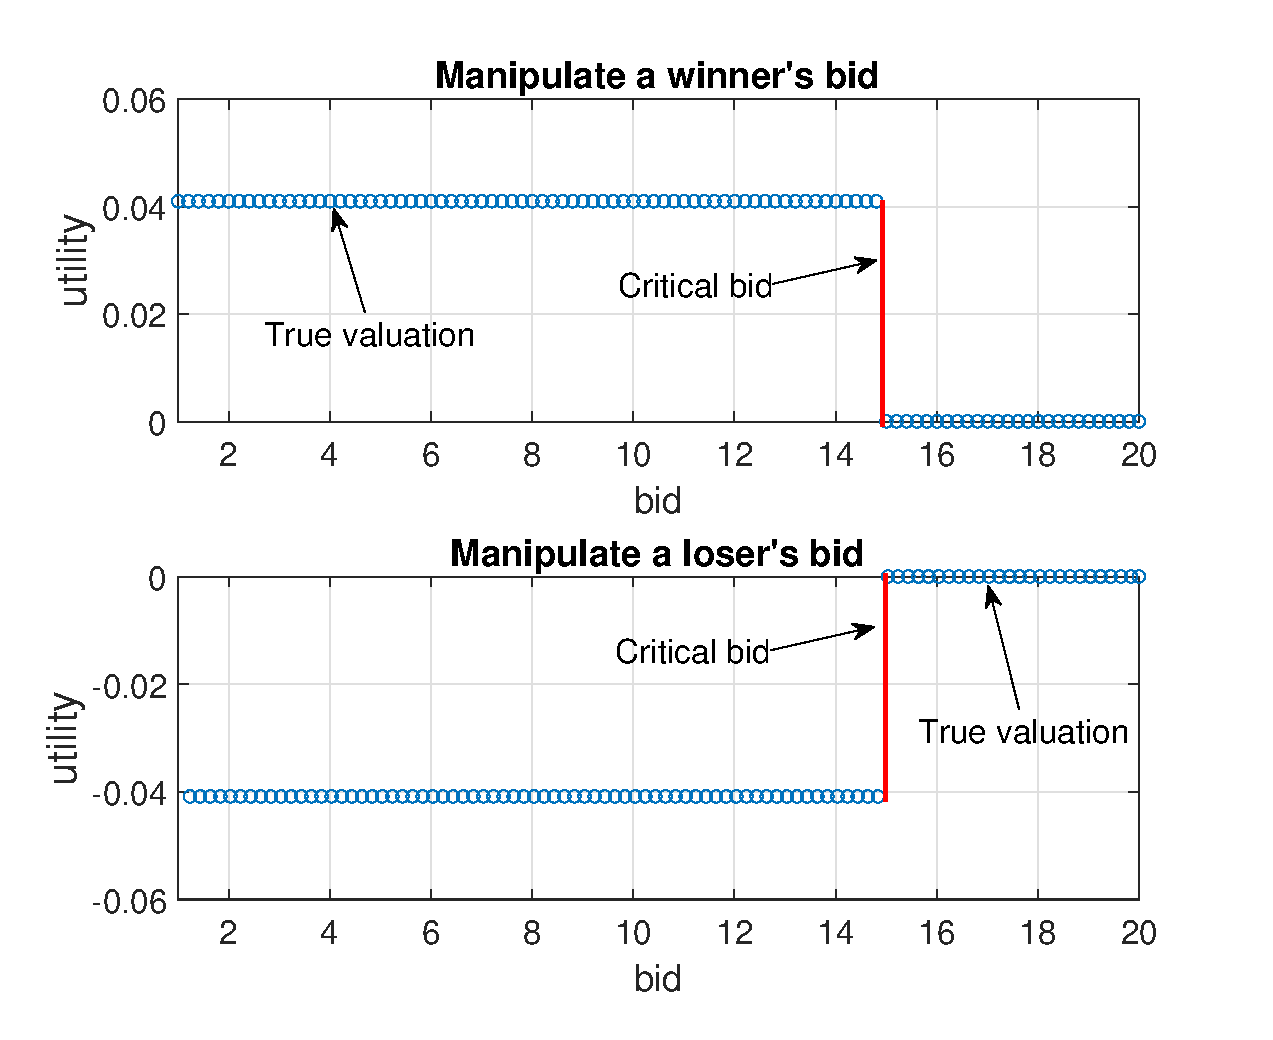
\includegraphics[scale=0.34]{./pic/truthfulness.eps}
%		\vspace{-0.2cm}
%		\caption{Truthfulness of the DPDA algorithm.}\label{fg:truthfulness}
%		\vspace{-0.0cm}
%	\end{figure}

\noindent{\textbf{计算复杂度}}
图\ref{fg:complexity}展示了算法DPDA的计算复杂度。对于$N$的每个取值,我们运行100次实验来评估算法的平均运行时间。实验中参数按节\ref{sec:setup}所述随机生成。我们实验所使用的PC配备有2.7GHz Intel Core i7处理器和16GB RAM。在不同的设置(即不同的失真度级别,出价和用户权重)下,我们观察到提出的DPDA算法的计算时间很短,并且与问题大小近似成线性关系。
%In Fig. \ref{fg:complexity}, we illustrate the computational complexity of the proposed DPDA algorithm. For each $N$, we examine the average running time of the algorithm by running 100 experiments, in which the parameters are randomly generated as mentioned in Section \ref{sec:setup}. These experiments are run on a PC with a 2.7 GHz Intel Core i7 processor and 16 GB RAM. Under different settings (i.e., different distortion levels, bids, and weights), we observe that the computation time of the proposed DPDA algorithm is low and approximately linear with the problem size.

	\begin{figure}[h!]
		\vspace{-0.2cm}
		\centering
		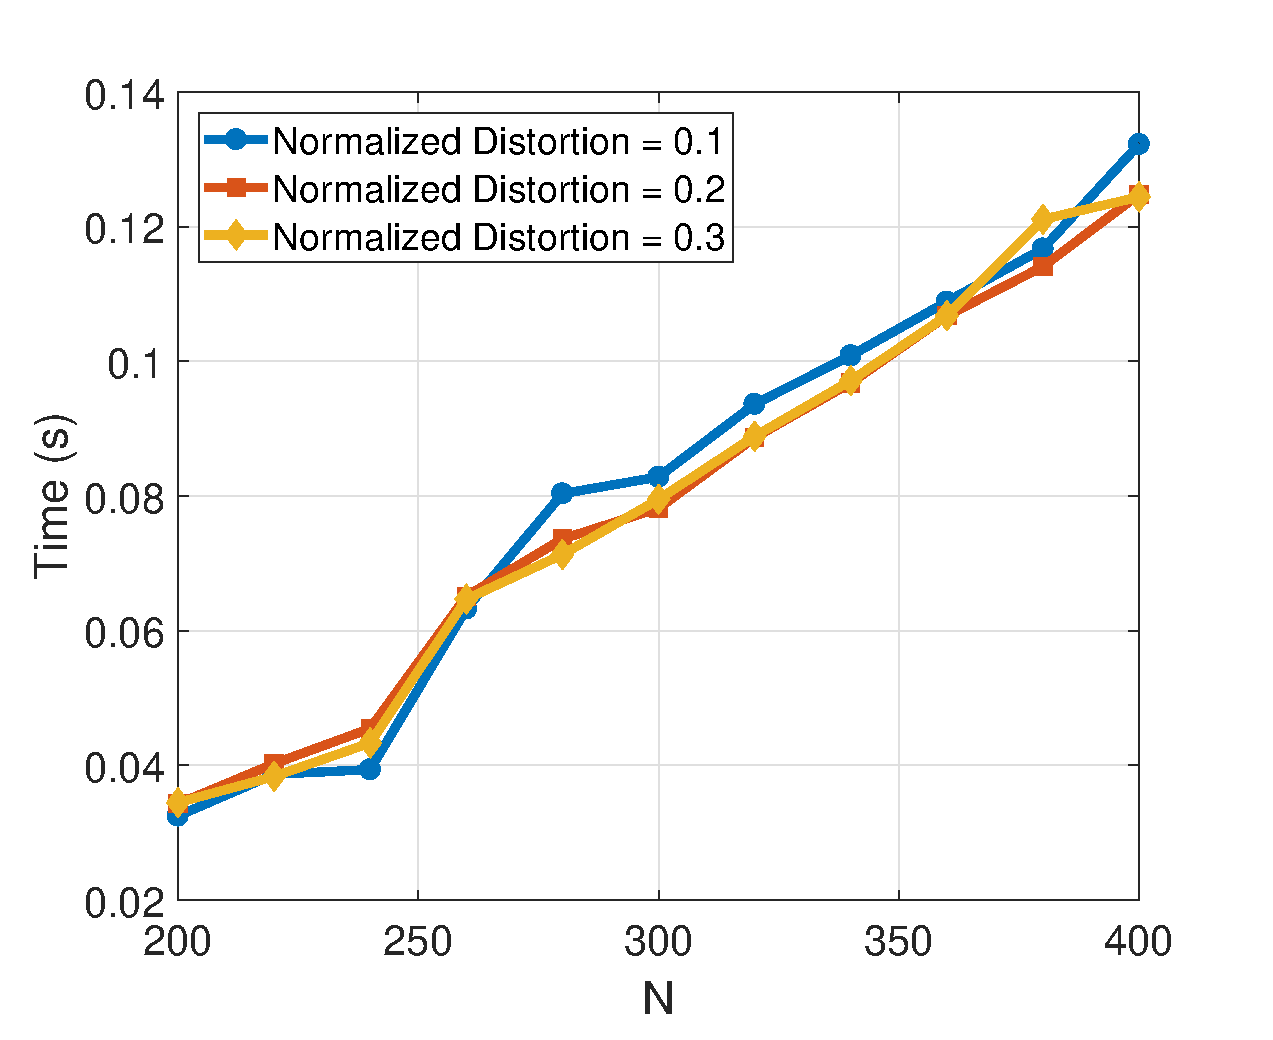
\includegraphics[scale=0.52]{./pic/complexity.eps}
		\vspace{-0.2cm}
		\caption{不同参数设置下DPDA的运算耗时。}\label{fg:complexity}
		\vspace{-0.3cm}
	\end{figure}

\section{本章小结}\label{sec:toncon}
本章在拍卖机制的框架下研究了隐私保护下的移动群智感知数据聚合问题,其中群智感知平台作为拍卖者征召移动用户来完成感知任务。在此模型下,本章应用差分隐私的概念设计了一种新颖的移动群智感知系统。具体来说,本章第2节提出了一种允许每个用户报告带有噪声数据的数据聚合方案,其中用户所允许添加的噪声分布由感知平台决定,使得用户的数据隐私保护程度可以通过差分隐私的量化指标进行衡量。本章第3节进一步提出了一个具有诚实性、个体合理性,且计算效率高的激励机制(DPDA)。该机制可以寻找到一组用户,在聚合结果准确性约束下,近似地将征召移动用户所需的成本降至最低。进一步,本章第4节将第3节提出的消极隐私保护框架泛化到一种积极隐私保护的场景。在这种场景中,用户可以通过竞标最低可接受的隐私保护级别来更好地控制其数据隐私保护级别。通过理论分析和充分的数值仿真,本文验证了DPDA算法和EDPDA算法的性能。
%We studied privacy-preserving data aggregation for mobile crowdsensing in an auction framework, where the platform plays the role as an auctioneer to recruit workers to complete a sensing task. Under this model, we designed a novel mobile crowdsensing system by leveraging the concept of differential privacy. Specifically, we designed a data aggregation that allows each worker to report a noisy data and can guarantee the use of each worker's data in a differentially private manner. Then, we designed a truthful, individual rational and computationally efficient incentive mechanism that can find a set of workers to approximately minimize the cost of purchasing the private sensing data from workers subject to the accuracy requirement of the aggregated result. We then generalize our results to a privacy-proactive scenario where workers could gain more control of their perceived data privacy protection level by beginning with bidding the lowest acceptable privacy level. We validated the performance of our proposed DPDA algorithm and EDPDA algorithm for the two scenarios through theoretical analysis as well as extensive simulations. 



%\chapter{具有社交意识的数据库辅助频谱访问:位置隐私、分布式学习和频谱共享}
\chapter{双重网络外部性下频谱共享网络吞吐量最大化研究}
\textbf{本章摘要:} 
在无线网络基础设施飞速发展的今天,随着移动用户数量的爆炸式增长,无线频谱资源短缺的问题已经日益凸显出来。数据库辅助频谱共享技术则长期以来被视为解决频谱短缺问题颇有前景的解决方案之一,尽管其在用户位置隐私保护方面的不足一直给用户带来担忧和顾虑。本章讨论了具有社交感知的数据库辅助频谱共享网络,其中移动用户在制定频谱共享决策时同时考虑其与附近用户在地理位置上的耦合(负网络外部性)以及其与社交好友在社交关系上的耦合(正网络外部性)。而为了应对基于RSS(Received Signal Strength)的网络物理层位置隐私攻击,本文采用了一种信号传输功率扰动的措施,允许每个次级用户巧妙地在传输功率水平上添加一个服从一定分布的负偏分量。本章第3节将这种隐私保护下的次级用户具有社交感知的频谱共享问题建模成一个随机信道选择博弈。博弈中次级用户作为策略性的玩家动态调整其策略,以最大化其社交群体效用。本章第4节进一步针对提出的博弈模型设计了一个基于无悔学习规则(No-regret learning rule)的双时间尺度分布式学习算法,并证明其几乎可以肯定收敛至博弈的相关均衡集合。本章第5节的数值结果证实,隐私保护级别越高,网络吞吐量的下降就越显着。

%Database assisted spectrum sharing is envisaged to be a promising solution to the spectrum shortage, caused by the immense growth of devices in both industrial and commercial wireless networks. Meanwhile, the lack of effective location privacy protection remains to be a concern for the potential participants in spectrum sharing. In this paper, we consider socially-aware database assisted spectrum access with location privacy protection, where mobile users jointly take into account their physical coupling (due to locational proximity) and social coupling while making spectrum sharing decisions. In particular, to mitigate RSS-based PHY-layer location privacy threat, we employ a power perturbation approach where each secondary user judiciously ``reduces'' its transmission power by choosing a power level following a statistical distribution (with a negative bias). Accordingly, we cast the privacy-preserving spectrum sharing among users as a stochastic channel selection game, where strategic players (secondary users) adjust their strategies dynamically aiming to maximize their social group utilities. Specifically, we devise a two-time-scale distributed learning algorithm based on no regret-based rule, and show that it converges almost surely to the set of socially-aware correlated equilibrium. The numerical results corroborate that the higher the privacy protection level, the more significant the degradation of the network throughput would be.

\textbf{关键词:}频谱接入;隐私保护;分布式算法;博弈论
%\keywords{毫米波通信;Massive MIMO;整数规划}

\section{引言}
在如今蜂窝网络频繁出现流量拥塞的现状下,如何解决爆炸性流量需求增长与有限网络资源间的冲突已经成为未来移动网络设计的主要挑战。针对这一挑战,世界各地的监管机构一直在积极研究动态频谱访问的政策法规以使频谱授权用户(主用户)和认知无线电设备(次级用户)通过协作实现互惠互利。在美国,联邦通信委员会(FCC)已经明确要求次级频谱用户需借助地理位置数据库来确定频谱的可用性\cite{FCCApril52012}。在这种数据库辅助的体系结构中,主用户将为数据库提供最新的频谱信息,从而无需次级用户对于未充分利用的频谱进行额外的检测\cite{db4}。
%The nowadays congested cellular networks has posed a significant challenge in mitigating the conflict of exploding traffic demand and limited resources for future wireless network design. To meet the rapidly growing demand of wireless traffic, regulatory agencies around the world have been actively working on policies and regulations for dynamic spectrum access that are mutually beneficial to the cognitive devices and the licensed spectrum users. Notably, the very recent FCC ruling requires that secondary TV spectrum users rely on a geo-location database to determine the  spectrum availability \cite{FCC}. In such a database-assisted architecture, the primary TV spectrum users provide the database with the up-to-date spectrum information, thereby obviating the need of sensing the underutilized spectrum \cite{db4}.
然而可靠的数据库辅助频谱接入目前仍然面临着诸多挑战。比如,次级用户的地理位置决定了其与周边用户之间的信号干扰,因而是用户进行频谱接入决策时主要考量的信息。而在数据辅助频谱接入中,这些可以被直接或间接地关联到用户个人隐私的地理位置信息尚未得到适当且有效的保护,给次级用户的隐私带来了严重的威胁。
%Nevertheless, reliable database assisted spectrum access remains challenging. Being critical to the users' spectrum access decisions, the geo-location information of secondary users can be linked to sensitive information of individuals, which, if not addressed adequately, would put secondary users' privacy at risk. 

学术界对于移动网络中用户位置隐私的保护已经进行了广泛的研究,其中一些主流的研究工作主要聚焦于网络应用层层面的隐私攻击与防护\cite{TII-crypo,TIE-DP}。
%There have been extensive studies on the protection of users' location privacy in wireless networks, most of which focus on privacy protection at the application layer \cite{TII-crypo,TIE-DP}. 
%(e.g., defending against an untrusted or compromised location-aware server). 
相比而言,针对网络物理层层面位置隐私攻击的相关研究仍然较少。实际中,基于在网络物理层面上的移动设备定位技术,隐私攻击者可以轻易的发起针对目标设备的位置隐私攻击。比如,攻击者可以从接收到的信号中提取相关参数,得到例如接收信号到达时间(TOA),到达时间差(TDOA),到达角度(AOA)和接收信号强度(RSS)\cite{TOARSS}的观测值,进而用来推断目标设备的位置。基于此观察,本章考虑一个攻击者模型,其中三个在目标用户周边不同位置的攻击者可以分别使用他们所接收到信号的RSS观测值来估计其与目标用户之间的距离,进而应用三角定位技术(例如文献[\citenum{Gezici:08}]中所使用的方法)完成对于目标用户的定位。

%Clearly, PHY-layer location privacy attacks deserve more attention because the physical signals often serve as the foundation for application development in practice. In fact, an adversary could easily extract physical-layer parameters (e.g., time of arrival (TOA), time difference of arrival (TDOA), angle of arrival (AOA), and received signal strength (RSS)\cite{TOARSS}) from the received signal, which can be utilized to infer the position of the target device. Based on this observation, we consider an adversary model that performs RSS-based localization attack at the PHY-layer. Specifically, an attacker can estimate the distance to the target secondary user using the RSS measurements of the received signal. Note that a set of three adversaries could jointly carry out the triangulation technique (e.g., the one introduced in \cite{Gezici:08}) to complete the localization of the target user. 

应对物理层位置隐私攻击的一种典型的策略是对攻击者用以进行位置推断的相关信号物理参数进行混淆处理\cite{Jiang07, EI10, Sangho12}。本章即采用了一种随机功率扰动的方法来应对基于RSS观测值的定位攻击。这其中每个用户会在原本给定的发射功率电平上添加一个根据特定分布采样得到的随机噪声分量。而使用扰动后的功率电平发送的信号将导致攻击者在信号接收时得到不准确的RSS观测值,从而有效降低其对于目标用户的定位精度。然而,尽管这种使信号发射功率偏离既定水平的方法具有较强的实用性,其不可避免地会导致网络性能的下降(例如,吞吐量的降低和延迟的增加)。因此,本文的主要目的是开发一种保隐私频谱共享机制,使其可以与功率扰动方法有效地结合起来使用,在网络性能优化与隐私保护之间寻求一种权衡。

%To mitigate the PHY-layer location privacy attacks, one basic idea (e.g., see \cite{Jiang07, EI10, Sangho12}) is to obfuscate the related parameters of signals that can be utilized by adversaries for position inference. In this work, we employ a random power perturbation approach to combat the RSS-based localization attack. To this end, each user's transmission power level consists of a given component and a stochastic noisy component generated from a particular distribution. The signal transmitted using the perturbed power level would lead to inaccurate RSS measurements at the adversary side, which could effectively reduce the localization accuracy of the target user. Despite its practicability, the random power perturbation approach we chosen would inevitably incur performance degradation (e.g., throughput and delay). Thus motivated, one primary goal of this study is to develop an effective spectrum sharing scheme that can be used in conjunction with the power perturbation approach.

对于数据库辅助频谱共享网络来说,实现网络性能优化的关键是如何协调次级用户之间的频谱接入,减轻同时接入相同空闲信道的用户之间所产生的干扰\cite{TII-game,TII-dynamic}。
基于实际中移动用户与所携带移动设备的强关联性,文献[\citenum{Chenjournal}]提出了一种名为“社交群体效用最大化”(SGUM)的博弈模型框架,用于求解针对具有社交关联的移动用户的网络效用最大化问题。在SGUM框架中,每个用户作为博弈的玩家会针对其他用户的策略调整自己的策略以最大化包含其自身效用以及其社交好友效用在内的“社交团体效用”。
%In addition to the privacy issue, another key challenge in effective database assisted spectrum access is how to coordinate the spectrum sharing among secondary users, so as to effectively mitigate the interference between users having access to the same vacant channel \cite{TII-game,TII-dynamic}. 
%Based on a key observation that mobile devices are associated with human beings, the authors in \cite{Chenjournal} developed a game-theoretic framework, named social group utility maximization (SGUM), for solving distributed network utility maximization over a group of socially connected users. In the SGUM framework, each user, interpreted as a player of the game, adjusts her strategy against others to maximize her `social group utility', which results in higher network utility. 

%Although the game theoretic modeling has been widely applied in spectrum resource management \cite{wang2010game}, this work is the first to investigate the socially-aware channel selection game under the threat of PHY-layer location privacy attack. Specifically, each user is allowed to transmit the signal using stochastic noisy power levels to degrade the localization accuracy. 
本章将隐私保护下的频谱接入问题表述为一个SGUM博弈。其中,次级用户在选择信道时同时考虑了其在物理域和社交域内与其他用户之间的耦合。为了应对基于RSS的定位攻击,每个用户将使用随机噪声功率电平进行数据传输,以混淆隐私攻击者对其的定位结果。
本文中通过分析博弈均衡解的特征来刻画博弈的动态特性。具体而言,本文使用了相关均衡(Correlated Equilibrium)的博弈均衡概念。相关均衡允许不同玩家的策略之间存在相关性,相比纳什均衡更具有一般性,并且有利于实际中的分布式实现\cite{Lasaulce2011}。
%Following \cite{Chenjournal}, we formulate the privacy-preserving spectrum access problem as a SGUM game in which secondary users take both physical aspect and social aspect into account while choosing a channel. To combat the RSS-based localization attack, each user is allowed to transmit the signal using stochastic noisy power levels to obfuscate the localization.
%We analyze the dynamics of the game based on the characterization of the equilibrium criteria. Specifically, we consider the correlated equilibrium (CE), a generalization of Nash equilibrium, which allows for dependencies among players' strategies and is easily amenable to distributed implementation \cite{Lasaulce2011}. 


%\begin{figure}[!t]
%%\hspace{-0.35cm}
%\centering
%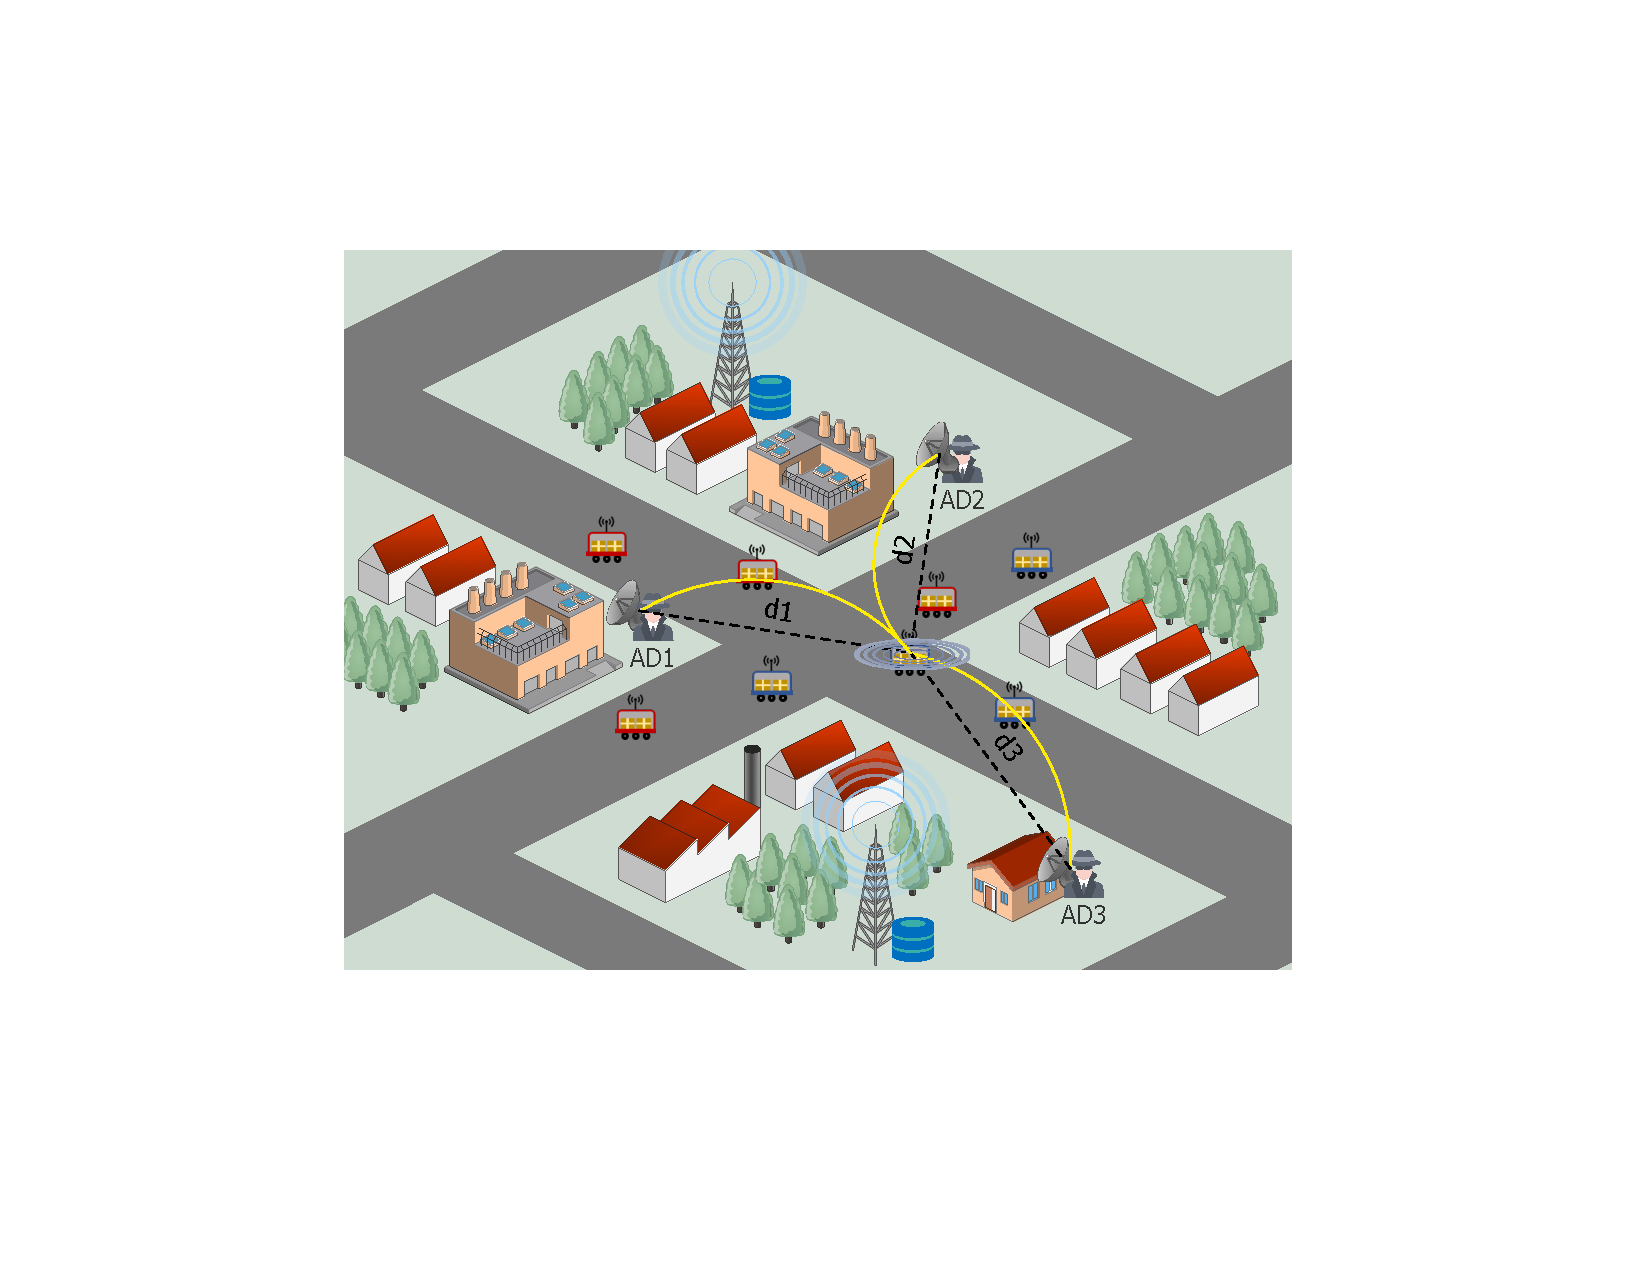
\includegraphics[scale=0.48]{./pic/Diagram22.pdf}
%\caption{An illustration of RSS based adversarial localization attack on an unmanned ground delivery system consisting of robotic vehicles belonging to two companies (differentiated by the colors). $d_1, d_2, d_3$ are distance estimations extracted from RSS measurements at three different positions, and are utilized to localize the target via trilateration technique.}\label{fg:trilate}
%\end{figure}
%
%With the expanding scale of IoT devices, the tremendous industrial data generated has put an increasing demand on bandwidth resources, which poses a significant challenge on the industrial spectrum management. To address the spectrum shortage, database-assisted spectrum access has been introduced where IoT are informed with the dynamic spectrum availability by a geo-location database, and access vacant licensed channels opportunistically \cite{TII-dynamic, TII-game}. The key challenge of dynamic spectrum access remains as how to coordinate the spectrum sharing in a distributed way, so that the mutual interference between devices having access to the same vacant channel can be effectively mitigated \cite{TII-game}. To this end, game theoretic models have been adopted for solving dynamic spectrum access problem, where devices are interpreted as selfish players making channel access decisions strategically to maximize their payoffs \cite{wang2010game}. 
%
%
%In addition to the spectrum scarcity, cyber-physical security remains to be another challenge for reliable operation of IIoT. As a main building block of industrial CPS, IIoT integrates the control, networking and computing components, providing fundamental supports for generation, collection and exchange of security-critical and privacy-sensitive data. The critical importance of IIoT makes itself an attractive and valuable target for cyber-physical attacks \cite{securitysuvey}. While extensive studies have been concerning the cyber-attacks and corresponding defenses, relatively less attention has been paid to the physical-layer attacks in IIoT. 
%%Among the many potential security attacks, the adversarial localization attack utilizing physical-layer information of victim's signals has been shown to be effective   []. 
%As a key vulnerability, the geo-location information of IoT devices, once being compromised, would put the device into great danger, which is extremely harmful for the reliability and safety of IIoT system. 
%
%In this study, we consider a practical RSS based adversarial localization attack that has been shown to be effective in pinpointing wireless IoT devices \cite{LocalizationLi}. 
%As illustrated in Fig. \ref{fg:trilate}, given a few RSS measurements collected within the vicinity of the victim, the adversary can easily carry out the localization attack using existing triangulation technique \cite{TOARSS}. Compared with localization approaches using other physical-layer informations (e.g., time of arrival (TOA), time difference of arrival (TDOA), angle of arrival (AOA) \cite{Gezici:08}), RSS based localization requires neither complex hardware nor active communication with the victim, which can be easily implemented by the adversary in practice.

%Many efforts have been made on developing countermeasures to mitigate physical-layer localization attacks, such as deploying directional antenna to limit transmission coverage \cite{antenna} and creating ghost locations to misguide adversaries via device-level cooperation \cite{Sangho12}. However, these approaches might be costly and difficult for widely system deployment, given the fact that IoT devices are generally of small size with limited computation and energy resources. Therefore, we consider using the light-weight power perturbation approach to combat the RSS based localization attack \cite{Jiang07}. The main idea behind is to add random noise to the transmission power level of IoT devices, with the aim to effectively lower the adversaries' localization accuracy \cite{EI10}. 
%
%Despite its practicability and effectiveness, the random power perturbation approach would result in inaccurate interference evaluation at IoT devices, which inevitably incurs performance degradation (e.g., throughput reduction) to the spectrum sharing system. Thus motivated, the goal of this study is to develop an effective spectrum sharing scheme in IIoT that can at the same time protect device's location privacy via transmission power perturbation. 
%
%Following \cite{Chenjournal}, we formulate the privacy-preserving spectrum access problem as a stochastic game where IoT devices update their channel selection choices dynamically with the objective of maximizing their utilities, as will be defined in Section \ref{sec:system-model}. 
%%To preserve the location privacy, IoT devices are allowed to judiciously add random noise to their transmission power levels.

为了在随机功率扰动影响下求解信道选择博弈的相关均衡(本文中简称为CE),本研究设计了一种双时间尺度的分布式学习算法。具体而言,在相对较大的时间尺度内,每个移动用户根据{\kaishu 带修正的无悔规则}\cite{Hart_areinforcement}来对其信道选择策略进行迭代。而在相对较小的时间尺度上,用户通过一个效用学习的动态过程不断更新其对于社交群体效用的估计,以解决由功率扰动引入的群体效用所含的随机噪声,提高在较大时间尺度上策略学习的效果。我们的分析指出,当学习过程的时间尺度满足一定温和的条件时,用户的联合决策的经验概率分布可以收敛于CE的集合。仿真结果验证得出,在随机功率扰动下,我们的双时间尺度学习算法优于仅使用信道选择策略自适应的单时间尺度学习算法。同时,评估结果表明我们所提出的双时间尺度学习算法有助于实现系统吞吐量和位置隐私保护之间的权衡。
%To solve for the CE of the channel selection game under the impact of random power perturbation, in this study we devise a two-timescale distributed learning algorithm. Specifically, at a slower timescale, each IoT device evolves her channel selection strategy according to a \emph{modified regret-based rule} \cite{Hart_areinforcement} using the locally maintained estimated utility. At a relatively faster timescale, the estimated utility keeps being updated via a learning process to address the randomness introduced by the power perturbation, which facilitates more effective strategy learning at the slower timescale. We show that under mild conditions on the learning timescales, the empirical frequency of users' joint actions converges to the set of CE. The simulation results show that, under the random power perturbation, our two-timescale learning algorithm outperforms the single timescale learning algorithm involving only the strategy adaptation of channel selection, which corroborates that the proposed two-timescale learning algorithm helps strike a balance between the system throughput and location privacy.

与大多数现有工作不同,本文的问题建模与求解过程中将频谱管理与用户位置隐私保护紧密地结合在一起。
%\cite{Bennis13}启发了提出的两时尺度学习算法的思想,该研究使用基于增强学习的算法研究了分散式小蜂窝网络中的干扰缓解。
%与我们较为相关的工作是\cite{ZhangGlobe},该文中作者使用博弈论模型研究了在具有社交意识的动态频谱访问情况下的位置隐私保护。在这项研究中,我们考虑了一个不同的均衡标准(即相关均衡),该标准通过放宽对玩家渠道选择策略的独立性假设来概括\cite{ZhangGlobe}中考虑的纳什均衡。此外,物联网设备旨在适应基于后悔规则\cite{Hart00asimple}的策略,而不是\cite{ZhangGlobe}中使用的随机虚拟对弈动态过程。
综上,我们的工作包含以下几点贡献:
%Summarizing, we have made the following contributions:
\begin{itemize}
\item 我们从双重网络外部性的视角阐释了频谱共享网络中存在的物理信号干扰(负网络外部性)与社交效应(正网络外部性),并通过社交群体效用函数的定义对两种效应进行了刻画。
\item 我们指出了在数据库辅助频谱接入系统中的基于RSS的位置隐私攻击隐患,并考虑了一种轻量级的功率扰动方法来降低隐私攻击者的定位精度。
%We identify the issue of RSS based adversarial localization attacks against IoT devices in database-assisted spectrum access, and consider a light-weight power perturbation approach to reduce the localization accuracy.
\item 我们通过一个隐私保护下信道选择博弈的建模来研究在动态频谱接入系统中进行位置隐私保护的问题。我们允许移动设备使用添加有扰动项的传输功率水平进行信号传输并策略性地做出信道选择决策以最大化其社交群体效用。
%We jointly study the dynamic spectrum access and location privacy protection by formulating a privacy-preserving channel selection game where IoT devices use perturbed transmission power level and strategically make channel selection decisions to maximize their utilities.
\item 我们提出了一种基于无悔学习规则的双时间尺度学习算法。该算法弱收敛于相关均衡集合,并且在用户使用随机功率扰动的情况下可以获得优于单一时间尺度学习算法的系统吞吐量指标。
%We propose a two-timescale learning algorithm based on regret learning rule, which converges weakly to the set of correlated equilibria and is shown to outperform the single timescale learning approach in alleviating the system throughput degradation from random power perturbation.
\end{itemize}
本章的其余部分安排如下。第\ref{sec:model}节首先介绍了隐私保护下具有社交意识的频谱共享的系统模型。第\ref{sec:game}节给出了用于频谱共享的SGUM博弈建模,并介绍了{\kaishu 无悔学习规则}(No-regret learning rule)。接下来,第\ref{sec:algorithm}节提出了隐私保护下频谱共享的双度尺度无悔学习算法,并在第\ref{sec:simulation}节中对算法的表现进行了评估。最后,第\ref{sec:con}节对本章进行了总结。
%The remainder of the paper is organized as follows. We first discuss the related work in Section \ref{sec:related}. In Section \ref{sec:model}, we describe the system model of socially-aware privacy-preserving spectrum sharing scheme. In Section \ref{sec:game}, we present the SGUM game formulation for spectrum sharing and introduce the no-regret based learning rule. Then we describe the two-time-scale regret-based learning algorithm for privacy-preserving spectrum sharing in Section \ref{sec:algorithm}, followed by the Section \ref{sec:simulation} which evaluates the effectiveness of the proposed algorithm. Finally, we conclude the paper in Section \ref{sec:con}.

%\section{研究现状}\label{sec:related}
%%Spectrum management techniques have been widely adopted into smart IIoT designs to meet the high QoS requirement for data communication, which helps to establish strong interconnection among industrial sensor, actuators and systems. For instances, Cao {\em et al.} in \cite{CaoCR} explored opportunistic accessibility of multiple channels to enhance the state estimation performance in a CPS with linear state dynamics. In \cite{TIICR}, Chiwewe {\em et al.} provided an overview of different techniques for spectrum management in cognitive radio based industrial wireless sensor network, and also explored the application of game theoretic modeling for spectrum sharing schemes.
%
%
%
%%We start with a brief review on related work on socially-aware spectrum sharing. Xing \emph{et al.}~proposed to use anthropological models in human society to enhance the performance of cognitive radio networks \cite{xing2008human}. Li \emph{et al.} \cite{li2011propagation} carried out social network analysis of the social behavior in cognitive radio networks. Another common approach for spectrum sharing based on social interactions is to model secondary users' interactions as noncooperative game (e.g., \cite{wang2010game} and many others) assuming they are \emph{selfish yet rational}. Notably, Chen \emph{et al.} \cite{chen2012spatial} developed a spatial spectrum access game framework to model the competitive spectrum access among the secondary users by taking the spatial reuse effect into account. 
%
%%Nie \emph{et al.} \cite{nie2005adaptive} designed a self-enforcing distributed spectrum access mechanism based on potential games. 
%%Law \emph{et al.} in \cite{law2009price} studied the system performance degradation due to the competition of secondary users in a distributed spectrum access game. 
%
%
%%Along a different avenue, industrial cyber-physical security issues have recently garnered much attention by both industry and academic communities, with great efforts focusing on the cyberattacks over industrial CPS \cite{securitysuvey}. In \cite{CPSsecurity}, the authors proposed a CPS security framework that distinguished the cyber, cyber-physical, and physical components in a CPS system, and surveyed over both potential and reported attacks as well as existing solutions. Particularly, in \cite{smartmeter}, the authors focused on the data privacy vulnerability of smart meters in smart grid system, and provided a thorough discussion on the state-of-the-art mitigation solutions. And in \cite{smartcity}, the authors discussed the the security and privacy challenges within emerging smart city applications such as intelligent healthcare and transportation system. 
%
%%By contrast, the adversarial localization attack considered in this study is a typical physical-layer attack targeting on wireless sensor networks in general \cite{Jiang07}. To combat such threats, one main approach is to obfuscate the physical information of the transmitted signal that can be potentially utilized by adversaries to infer the users' locations. In \cite{Jiang07} and \cite{EI10}, mobile devices were designed to strategically reduce their transmission power so as to reduce the number of adversaries that can collaboratively carry out RSS-based localization attacks, or to degrade the accuracy of the adversarial localization. In \cite{Ting11}, 
%%Oh {\em et al.} \cite{Sangho12} and Taha {\em et al.} \cite{Xuemin13} proposed solutions that create fake locations to mitigate the RSS-based localization attacks. 
%
%近些年来,有关于无线网络中位置隐私保护的相关问题获得了极大的关注。
%%Along a different avenue, location privacy has recently garnered much attention with great efforts focusing on privacy protection  at the application layer. 
%%The major approaches include location obfuscation (e.g., \cite{Agrawal:Privacy}), anonymization (e.g., \cite{Beresford:Mix, Gongjournal, Shin:AnonySense}), differential privacy (e.g., \cite{Dwork:Differential}) and cryptographic-based transformation (e.g., \cite{Ghinita:Private, Khoshgozaran:Blind}), each being suitable for different type of applications. 
%%Location-obfuscation schemes perturb users' location information by adding random noises to their locations. In anonymization, there are two different approaches: pseudonym (e.g., \cite{Beresford:Mix}) and $k$-anonymity (e.g., \cite{Shin:AnonySense}). The former decouples the link between users' real identity and their location information, while the latter ensures that there are at least $k$ users whose locations are indistinguishable. Differential privacy protects the information of each individual in the database while publishing statistical information (e.g., average) about the database. Cryptographic-based transformation encrypts users' location information to make it confidential. 
%%Nevertheless, these application-layer solutions have very limited effectiveness against the physical-layer location privacy attacks in wireless networks, which aim at localizing users based on the measurements of their transmitted signals.
%在一些网络物理层的位置隐私攻击模型中,攻击者主要利用信号的物理信息来推断用户的位置。因而使传输信号的物理信息变得模糊成为了一种防御物理层位置隐私攻击的主要手段。在\cite{Jiang07}和\cite{EI10}中,移动设备通过策略性地降低其传输功率,从而可以有效减少可参与协作进行RSS定位的攻击者数量,或降低攻击者RSS定位的准确性。 Wang等\cite{Ting11}则着重于定向天线的设计,以解决物理层位置隐私攻击的问题。Gao等\cite{location}所应用的位置隐私保护措施与本文中所使用的较为接近。然而与本文所考虑的基于RSS的定位攻击不同,\cite{location}中考虑的是通过推断目标用户所使用的信道来判断其位置。因而目标用户可以通过选择最有利的信道来缓解隐私攻击的威胁。
%%As for the physical-layer location privacy attacks in wireless networks, one main approach is to obfuscate the physical information of the transmitted signal that can be potentially utilized by adversaries to infer the users' locations. In \cite{Jiang07} and \cite{EI10}, mobile devices are allowed to strategically reduce their transmission power so as to reduce the number of adversaries that can collaboratively carry out RSS-based localization attacks, or to degrade the accuracy of the RSS-based localization. Wang {\em et al.} focused on the design of directional antenna to address the physical-layer location privacy attacks. In \cite{location}, Gao {\em et al.}  considered the location privacy protection in a cognitive radio network similar to ours. While instead of the RSS-based attack, they considered an attack model that inferred a secondary user's location through her used channels, and the threat was mitigated by choosing channels in favor of the most stable ones.
%
%与大多数现有工作不同,本文我们共同考虑频谱管理和位置隐私保护。\cite{Bennis13}启发了提出的两时尺度学习算法的思想,该研究使用基于增强学习的算法研究了分散式小蜂窝网络中的干扰缓解。也许与我们最相关的工作是\cite{ZhangGlobe},它使用博弈论模型研究了在具有社交意识的动态频谱访问情况下的位置隐私保护。在这项研究中,我们考虑了一个不同的均衡标准(即相关均衡),该标准通过放宽对玩家渠道选择策略的独立性假设来概括\cite{ZhangGlobe}中考虑的纳什均衡。此外,物联网设备旨在适应基于后悔规则\cite{Hart00asimple}的策略,而不是\cite{ZhangGlobe}中使用的随机虚拟游戏动力学。
%%Different from most of the existing works, in this paper we jointly consider the spectrum management and locational privacy protection. The idea of the proposed two-timescale learning algorithm is inspired by \cite{Bennis13}, which studied the interference mitigation in decentralized small-cells networks using a reinforcement learning based algorithms. Perhaps The most related work to ours is \cite{ZhangGlobe}, which investigated the location privacy protection under the scenario of socially-aware dynamic spectrum access by using game theoretic modeling. In this study, we consider a different equilibrium criteria (i.e., correlated equilibrium) which generalizes the Nash equilibrium considered in \cite{ZhangGlobe} by relaxing the independence assumption on the players' channel selection strategies. In addition, the IoT devices are designed to adapt strategy following the regret-based rule\cite{Hart00asimple} instead of the Stochastic Fictitious Play dynamics used in \cite{ZhangGlobe}. 
%
%%\section{System Model for Locational Privacy Preserving Spectrum Sharing}\label{sec:model}
\section{位置隐私保护下的频谱共享系统模型}\label{sec:model}


%\subsection{Basic Setting}\label{sec:system-model}
\subsection{基本设置}\label{sec:system-model}
根据FCC\cite{FCCApril52012}的规定,在数据库辅助频谱访问中,每个空白用户将首先向数据库发送频谱访问请求,然后数据库将向该用户显示在特定位置处空闲的TV信道。我们考虑这样的一个由主信道(例如电视频道)频谱集合$\mathcal{M}athcal{A}=\{1,2,\cdots,M\}$组成的频谱接入网络。在这个网络中有一组次级用户$\mathcal{M}athcal{V}=\{1,2,\cdots,N\}$会去尝试在信道未被主用户占用的情况下访问这些空闲的信道。具体来说,每个用户$n\in\mathcal{M}athcal{V}$可以访问数据库公布的一个可用信道子集$\mathcal{M}_n\subseteq\mathcal{M}athcal{A}$。显然,如果次级用户之间没有适当的协调,则可能会发生信道使用的冲突,且所产生的信道干扰会严重影响网络的性能。 {\kaishu 因此,在存在时变信道占用和干扰的环境中,数据库辅助频谱接入可以被归结为次级用户之间的动态信道分配。}
%According to the recent ruling by FCC \cite{FCC}, in database-assisted spectrum access, each white-space user will first send a spectrum access request to a database, and the database will reveal the vacant TV channels at a particular location to that user. We consider such a spectrum access network with a set $\mathcal{M}athcal{A}=\{1,2,\cdots,M\}$ of primary channels (e.g., TV channels). And a set $\mathcal{M}athcal{V}=\{1,2,\cdots,N\}$ of secondary users (i.e., IoT devices) try to access these channels when the channels are not occupied by licensed users. In particular, each user $n\in\mathcal{M}athcal{V}$ can access a subset of available channels $\mathcal{M}_n\subseteq\mathcal{M}athcal{A}$, as revealed by the database. Apparently, without proper coordination among secondary users, the conflict on channel usage may occur, and the generated interference could severely degrade the network performance. {\em Accordingly,  database-assisted spectrum access boils down to the dynamic channel allocation among secondary users, in a time-varying channel occupancy and interference environment.}
\begin{figure}[!t]
%\hspace{-0.35cm}
\centering
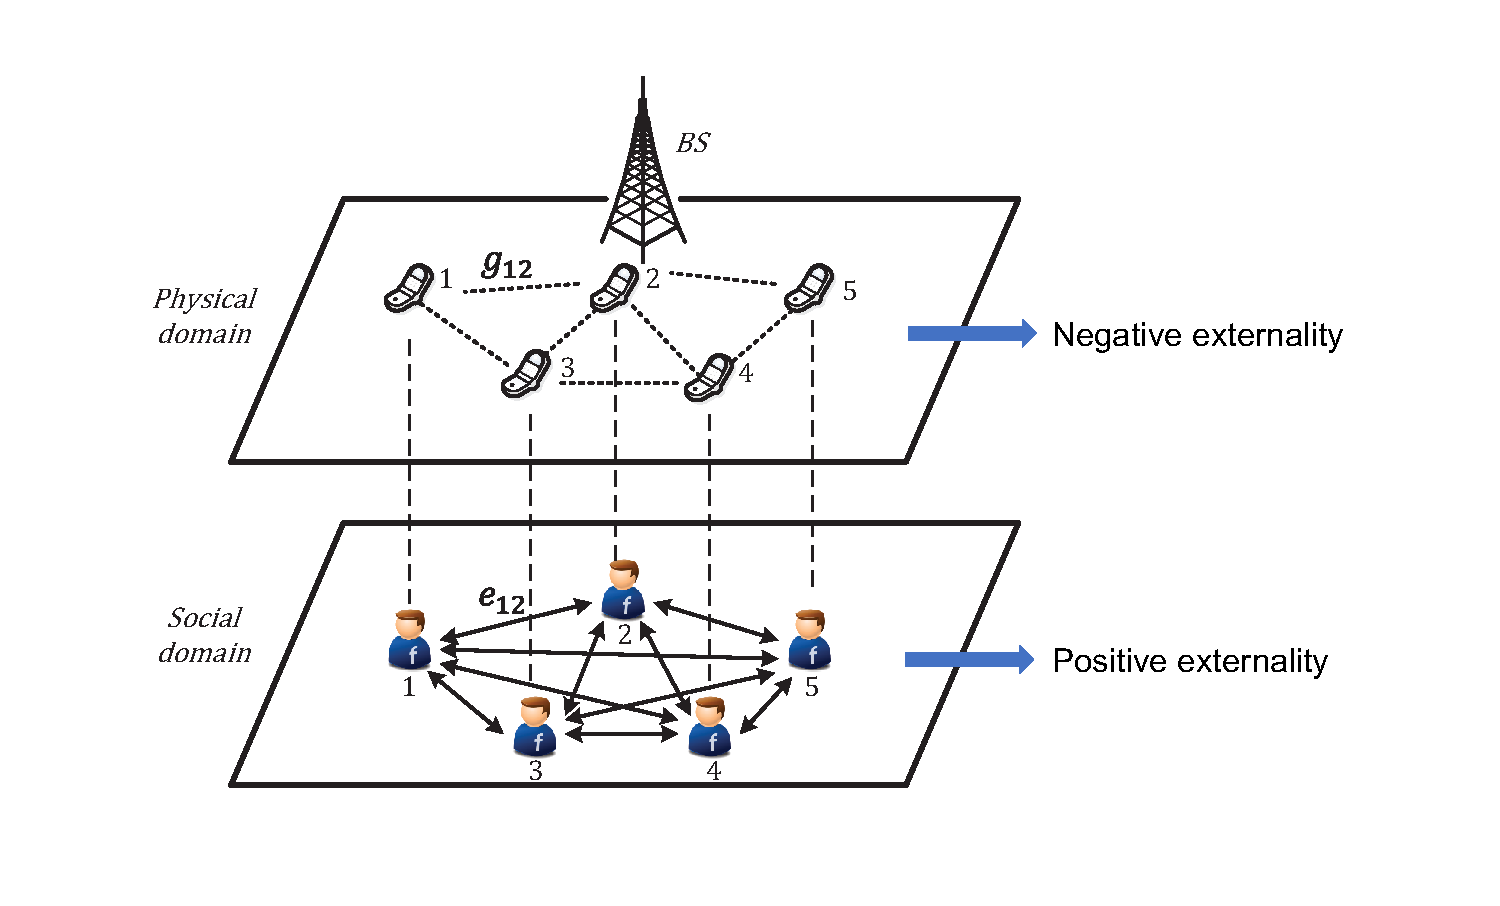
\includegraphics[scale=0.64]{./pic/sysfig11.pdf}
\caption{认知无线电网络的社交域-地理域说明}\label{fg:domain}
\end{figure}

参照文献\cite{Chenjournal},我们考虑一个具有社交意识的认知无线电网络(如图\ref{fg:domain}所示),其中每个次级用户在选择频道时都考虑了地理位置和社交关系所决定的双重网络外部性的影响。
%Following \cite{Chenjournal}, we consider a socially-aware cognitive radio network (as illustrated in Fig. \ref{fg:domain}), where each secondary user takes both physical and social aspects into account during channel selection. 
%In particular, the social relationships among secondary users are leveraged to facilitate cooperation in spectrum sharing. 
一方面,由于数据传输产生的信道干扰,次级用户在地理域中耦合,并希望通过减弱干扰来增加其传输效用。而接入同一信道的用户越多,单一用户的效用越差(负网络外部性)。另一方面,次级用户通过他们之间的社交联系在社交域中相互耦合。由于用户的大部分通信流量产生于同社交好友之间的互动,因此社交好友通信吞吐量的提升对于用户个人的效用带来非直接的正向影响(正网络外部性)。对于具有社交意识的次级用户,在进行通信时考虑与其有社交联系的其他次级用户的效用,将形成一种双赢的局面。
%On the one hand, secondary users are coupled in the physical domain due to the interference relationship in data transmissions, and would like to increase their utilities through interference mitigation. On the other hand, secondary users are coupled in the social domain via the social ties among them. It would be a win-win case for socially-aware secondary users to consider the utilities of those users having social trust with him (her).

我们使用一个信道干扰模型来刻画设备之间的地理位置上的耦合。具体来说,我们令$a_n\in\mathcal{M}_n$表示为用户$n\in\mathcal{M}athcal{V}$所访问的信道,并将其通信链接上的信道增益表示为$g_{nn}^{a_n}$。然后我们令$g_{mn}^{a_n}$表示用户$m\in\mathcal{M}athcal{V}$和用户$n$的通信链路之间在信道$a_n$上的干扰增益。我们用$N_{a_n}$表示用户$n$的链路在信道$a_n$上的噪声,对应的信噪比(SINR)$\gamma_n(P_n)$可以表示为
%To capture the physical coupling among devices, we assume a physical interference model. Specifically, we denote $a_n\in\mathcal{M}_n$ as the channel that user $n\in\mathcal{M}athcal{V}$ have accessed, and denote the channel gain on her communication link as $g_{nn}^{a_n}$. We then let $g_{mn}^{a_n}$ denote the channel gain of $a_n$ over the interference link between user $m\in\mathcal{M}athcal{V}$ and user $n$. The noise of channel $a_n$ on the link of user $n$ is denoted as $N_{a_n}$. The Signal-to-Interference and Noise Ratio (SINR) $\gamma_n(P_n)$ of user $n$ can be written as
\begin{equation}
\small
\gamma_n(P_n)=\frac{P_{n}g_{nn}^{a_n}}{\sum_{m\in \mathcal{M}athcal{V}/\{n\}}P_{m}g_{mn}^{a_n}\mathcal{M}athds{1}_{\{a_m=a_n\}}+N_{a_n}},
\end{equation}
其中$P_n$是用户$n$使用的传输功率;当用户$m$和用户$n$访问同一信道时,指示函数$\mathcal{M}athds{1}_{\{a_m = a_n\}}$等于1,反之等于零。我们用$W$表示带宽,并将功率水平为$P_n$时的吞吐量定义为用户$n$的个体效用函数,即
%where $P_n$ is the transmission power used by user $n$; the indicator function $\mathcal{M}athds{1}_{\{a_m=a_n\}}$ is equal to 1 when user $m$ and user $n$ access to the same channel (i.e., $a_m=a_n$), and zero otherwise. We let $W$ denote the bandwidth, and define the individual utility of user $n$ as her throughput with power level $P_n$,
\vspace{-0.2cm}
\begin{equation}\label{indiu}
U_n=W\log[1+\gamma_n(P_n)].
\end{equation}

我们使用无向社交图$G^S=\{\mathcal{M}athcal{V},E\}$来对用户之间的社交耦合进行建模。其中每个顶点对应于集合$\mathcal{M}athcal{V}$中的一个用户,用图中无向的边表示用户之间的社交关系。特别的,我们对于联结任意两个用户$n$和$m$的边赋予一个权重$e_{nm}\in [0,1]$来量化两个用户之间社交关系的亲密程度。此外,我们所定义的权重具有以下特性:$e_{nm}=e_{mn},e_{nn}=1, \forall n,m\in\mathcal{M}athcal{V}$。
%The social coupling among users is modeled by using an undirected social graph $G^S=\{\mathcal{M}athcal{V},E\}$, with each vertex corresponding to a user within set $\mathcal{M}athcal{V}$, and undirected edges indicating the social relationship among users. In particular, we assign a weight $e_{nm}\in [0,1]$ to the edge connecting two arbitrary users $n$ and $m$ to quantify the closeness of the social relationship between the two users. Further, the edge weights have the following characteristics: $e_{nm}=e_{mn},e_{nn}=1, \forall n,m\in\mathcal{M}athcal{V}$.
%\subsection{Social Group Utility Maximization (SGUM) for Spectrum Access}
%As hand-held devices are carried by human beings, the social relationships among users can be leveraged to enable such collaborations among users. Intuitively, by taking into consideration of the social aspect, users are expected to select channels more wisely instead of in a fully selfish manner. 
我们使用社交群体效用模型来刻画存在社交联系的设备之间潜在的社交耦合,在这里,我们定义用户$n$的社交群体效用函数为
\vspace{-0.2cm}
\begin{equation}\label{sgu}
S_n=U_n+\sum_{m\in \mathcal{M}athcal{V}/\{n\}}e_{nm}U_m.
\end{equation}
该定义中用户的个体效用刻画了用户间的{\kaishu 负网络外部性}影响,而对于社交好友个体效用的加权求和则刻画了用户之间的{\kaishu 正网络外部性}效应。
%。直观地,$e_n$的值越大,设备$n$与其所关联的群体之间的社交联系越强。
%We use such a group utility model to capture the underlying social coupling among homogeneous IoT devices within the same group. Intuitively, the larger the value of $e_n$, the stronger the social connection that device $n$ has with respect to the group she is associated with.


%\subsection{Random Power Perturbation against RSS-based Location Privacy Attack}\label{sec:privacy-model}
\subsection{针对基于RSS的位置隐私攻击的随机功率扰动}\label{sec:privacy-model}
\subsubsection{基于RSS的位置隐私攻击}
在这项研究中,我们考虑了一个物理层攻击者模型,该模型采用基于接收信号强度(RSS)的定位技术来获取目标用户的位置隐私。基于RSS的定位可以捕获传输的信号,并可以根据信号传播模型\cite{Jiang07,EI10}建立距离与RSS之间的映射。每个攻击者可以采集一系列目标用户发射信号的RSS电平\footnote{例如,通过采集信号RSS并结合RF指纹技术\cite{TIEYuanchao},信号接收者可以通过分析信号模拟分量中的瑕疵来识别无线网卡。},并使用通过最大似然估计\cite{RSSguang}获得距离的估计。
%In this study, we consider a PHY-layer adversary model that employs the Received Signal Strength (RSS) based localization technique to compromise target users' location privacy. RSS-based localization captures the transmitted signal and can establish the mapping between the distance and the RSS according to the signal propagation model \cite{Jiang07,EI10}. As illustrated in Fig. \ref{fg:trilate}, each adversary can collect a sequence of RSS levels of the transmitted signal from the target user\footnote{For instance, through the RF fingerprint technique\cite{TIEYuanchao}, a receiver can identify a wireless card by analyzing imperfections in the analog components of the signal.}, and obtain an estimation of the distance using via Maximum Likelihood estimation \cite{RSSguang}. 
%According to the propagation model (e.g., the log-normal model), each adversary can obtain an estimation of the distance between the target user and herself.  sequence of RSS measurements
然后,攻击者可以通过使用一组距离估计结合其自身地理位置使用三角测量的方法近似地确定目标用户的位置。
%Then an approximate location of the target user can be jointly determined by a trilateration using a set of distance estimations and the corresponding physical positions of the adversary.


\subsubsection{传输功率随机扰动}
为了对抗基于RSS的位置隐私攻击,我们采用了一种本地传输功率随机扰动的方法,旨在增加攻击者定位结果的不确定性\cite{EI10}。为此,每个用户可以动态地随机改变其传输功率水平。攻击者收集到的带有噪声的RSS测量值会有效地扩大目标用户定位的不确定性区域,从而降低定位精度。
%To combat RSS-based location privacy attack, we employ a local random power perturbation approach aiming to introduce uncertainties to adversaries' localization outcome\cite{EI10}. To this end, each user is allowed to dynamically and randomly change her transmission power level on purpose. The noisy measurements of RSS obtained at the adversary could effectively enlarge the uncertainty region of target user's position, which reduces the localization accuracy.

为了避免对主用户的额外干扰,我们限制随机功率扰动分量为负偏值。具体来说,用户$n$扰动后的传输功率可表示为$P_n=p+\Delta p_n$,即常规传输功率电平$p> 0$和扰动项$\Delta p_n$的加和。扰动项可被表示为一个服从单边截断指数分布的随机变量,其概率密度函数的表达式为
%To avoid extra interference to the primary users, we restrict the random power perturbation component to be negative biased. Specifically, the perturbed transmission power of user $n$ is given by $P_n=p+\Delta p_n$, which is the sum of the regular transmission power level $p>0$ and a perturbation term $\Delta p_n$, generated following one-side truncated exponential distribution whose \emph{pdf} is given as
\begin{equation}\label{eq:noise}
%\small
f(\Delta p_n|b,\bar{p})=\frac{\frac{1}{b}\exp(\Delta p_n/b)}{1-\exp(\bar{p}/b)},~\Delta p_n\in(-\bar{p},0],
\end{equation}
其中$\bar{p}$表示最大扰动量。当扰动超出该范围时,将导致SINR过小而不满足正常数据传输的要求。参数$b>0$则刻画了用户指定的一个“平均”功率扰动水平,我们将在节\ref{sec:simulation}中对其做进一步讨论。

%with $\bar{p}$ denotes the maximum perturbation level beyond which the SINR of IoT device might be unacceptable for normal data transmission. The parameter $b>0$ characterizes the ``expected'' power perturbation level specified by the user, as will be further discussed in Section \ref{sec:simulation}.

%\section{Socially-aware Privacy-preserving Spectrum Sharing}\label{sec:game}
\section{隐私保护下带有社交意识的频谱共享}\label{sec:game}
在本节中,我们将频谱共享问题转换为社会团体效用最大化(SGUM)博弈,并介绍了无悔学习规则,该规则可以以分布式方式计算非合作博弈的相关均衡。
%In this section, we cast the spectrum sharing problem as a social group utility maximization (SGUM) game, and introduce the no-regret matching rule, which can calculate the correlated equilibrium of a non-cooperative game in a distributed manner.

%\subsection{Social Group Utility Maximization (SGUM) Game for Spectrum Sharing}\label{sec:SGUM}
\subsection{频谱共享中的社交群体效用最大化(SGUM)博弈}\label{sec:SGUM}
在我们的研究中,我们将系统中的每一对接收发射端视为一个用户,他们之间存在持续的策略性的交互,旨在从长远来看最大化他们各自的社交群体效用。
为此,我们将隐私保护下的频谱共享问题建模为一个社交群体效用最大化(SGUM)博弈,每一个用户对应于博弈中的一个玩家\footnote{是本章中,术语上“用户”和“玩家”可以互换。}。
%In our study, all the transmitter-receiver pairs in the system are modeled as self-interested users interacting strategically and repeatedly with each other, aiming to maximize their social group utilities in the long run. 
%To this end, we formulate the privacy-preserving spectrum sharing problem as a \emph{social group utility maximization (SGUM) game} with the players corresponding to the users\footnote{We use the terms ``user'' and ``player'' interchangeably throughout the paper.}.
%In addition, each $TR$ will actively perturb her transmission power in order to mitigate the threat of RSS based location privacy attack.
每个玩家$n\in\mathcal{M}athcal{V}$的行为空间在这里被定义为用户$n$可以接入的可用信道集合$\mathcal{M}_n$。我们令$\A=(a_1,a_2,\cdots,a_N)\in\mathcal{M}$表示所有用户的联合频谱接入选择方案,其中$\mathcal{M}\triangleq\prod_{n=1}^N\mathcal{M}_n$。
%The action space of each player $n\in\mathcal{M}athcal{V}$ is the set of available channels $\mathcal{M}_n$ that user $n$ can access. We let $\A=(a_1,a_2,\cdots,a_N)\in\mathcal{M}$ denote the joint spectrum access profile of all the users, where $\mathcal{M}\triangleq\prod_{n=1}^N\mathcal{M}_n$. 
%Since the observed social group utility is noisy due to the power perturbation implemented by each user, it makes more sense for each user to target on maximizing its 
为了便于评估每个用户的长期社交群组效用期望,我们令$\Delta\mathcal{M}_n$表示用户$n$的混合策略空间,并令$\pi_n=\left(\pi(a_{n,1}),\pi(a_{n,2}),\cdots,\pi(a_{n,|\mathcal{M}_n|})\right)\in\Delta\mathcal{M}_n$表示用户$n$的混合策略。其本质上可看作为是定义在$\mathcal{M}_n$上的一个概率分布,其中$q(a_{n,i})$代表用户选择信道$a_{n,i}$的概率。因此,所有玩家的联合混合策略可以被表示为$\p=(\pi_1,\pi_2,\cdots,\pi_N)\in\Delta\mathcal{M}\triangleq\prod_{n=1}^N\Delta\mathcal{M}_n$,而按照管理除用户$n$外的其他玩家的联合策略可以表示为$\p_{-n}=(\pi_1,\cdots,\pi_{n-1},\pi_{n+1},\cdots,\pi_N)$ 。我们进一步令$\pi(\A)$表示联合决策$\A\in\mathcal{M}$在博弈中出现的概率。


%To facilitate the evaluation of each user's long-term expected group utilities, we denote $\Delta\mathcal{M}_n$ as the mixed strategy space of user $n$, and let $\pi_n=\left(\pi(a_{n,1}),\pi(a_{n,2}),\cdots,\pi(a_{n,|\mathcal{M}_n|})\right)\in\Delta\mathcal{M}_n$ denote user $n$'s mixed strategy, a probability distribution over $\mathcal{M}_n$ with $q(a_{n,i})$ representing the probability of selecting the channel $a_{n,i}$. It follows that the joint mixed-strategy over all players is $\p=(\pi_1,\pi_2,\cdots,\pi_N)\in\Delta\mathcal{M}\triangleq\prod_{n=1}^N\Delta\mathcal{M}_n$, and the joint strategy of players excluding user $n$ can be denoted as $\p_{-n}=(\pi_1,\cdots,\pi_{n-1},\pi_{n+1},\cdots,\pi_N)$ by convention. We further denote $\pi(\A)$ as the probability of joint action $\A\in\mathcal{M}$ being played. 

基于以上模型,我们将隐私保护下的频谱共享问题视为一个非合作信道选择博弈,用一个三元组$\Gamma=\left(\mathcal{M}athcal{V},\Delta\mathcal{M},\{S_n\}_{n=1}^N\right)$来表示,博弈中每个玩家旨在最大化自身的期望社交群体效用。我们研究中考虑的均衡标准是{\kaishu 相关均衡(Correlated Equilibrium)}。由于相关均衡允许不同玩家的之间的策略存在相关性,因此可被看做是{\kaishu 纳什均衡(Nash Equilibrium)}的一个泛化。数学上来看,一个相关均衡对应一个凸多面体,凸面体的极值点对应于纳什均衡。因此,通常系统可以在达到相关均衡时比达到纳什均衡时获得更好的总体性能。
%Summarizing, we cast the privacy-preserving spectrum sharing problem as a non-cooperative game denoted by a 3-tuple $\Gamma=\left(\mathcal{M}athcal{V},\Delta\mathcal{M},\{S_n\}_{n=1}^N\right)$. The equilibrium criteria considered in our study is the \textsl{correlated equilibrium}, which generalizes the Nash equilibrium by permitting players' strategies to be dependent. Mathematically, a correlated equilibrium is a convex polytope with its extrema points corresponding to the set of Nash equilibria. Thereby, in general, a better overall performance can be achieved under the correlated equilibrium than that under a Nash equilibrium. 
我们在下面给出相关均衡的正式定义。
%The formal definition of correlated equilibrium is given below.


\begin{df}[相关均衡]
我们称定义在$\Delta\mathcal{M}$上的概率分布$\pi^*$为信道选择博弈$\Gamma$的一个相关均衡(CE),如果$\forall n\in\V$,$\forall a_{n,i},a_{n,j}\in\mathcal{M}_n$,社交群体效用$S_n$满足以下不等式,
%A probability distribution $\pi^*$ on $\Delta\mathcal{M}$ is a socially-aware correlated equilibrium (CE) of game $\Gamma$ if, $\forall n\in\V$, $\forall a_{n,i},a_{n,j}\in\mathcal{M}_n$, the expected group utility satisfies the following,
\begin{equation}
\sum_{\textbf{a}\in\mathcal{M}:a_n=a_{n,i}}\pi^*(\textbf{a})\left[S_n(a_{n,j},\textbf{a}_{-n})-S_n(\textbf{a})\right]\leq0.
\end{equation}
\end{df}

\noindent{\bf 备注}
为了获得对相关均衡更具体理解,我们可以将$\pi^*$看作频谱数据库提供的一个信道接入策略推荐。则对于每个用户而言,假设其他用户都遵循频谱数据库所推荐的相应均衡策略,则同样遵循频谱数据库所推荐的策略会是对于该用户最有利的选择。换句话说,用户不能依靠单方面背离CE推荐的策略获得期望社交群体效用的提升。
%To get a concrete sense of the correlated equilibrium herein, one can view $\pi^*$ as a strategy recommendation provided by the trusted spectrum database. With the implicit assumption that other users' strategies follow the given recommendation, it is of best interest of each user to also follow the recommended strategy. In other words, a user could not obtain a better expected group utility by deviating from the CE unilaterally. 

\begin{thm}(CE的存在性)
信道选择博弈$\Gamma$至少存在一个相关均衡(CE)。
%There exists at least a SCE in the stochastic channel selection game $\Gamma$.
\end{thm}
由于我们的信道选择博弈$\Gamma$中的玩家集合和策略集合都为有限集,因此属于有限博弈的范畴,继而保证存在一个非空的相关均衡集合\cite{Lasaulce2011}。
%Since our channel selection game $\Gamma$ consists of finite player set and action set, it falls into the category of finite game, which is guaranteed to possess a nonempty set of correlated equilibria\cite{Lasaulce2011}.


\subsection{无悔学习规则(No-regret learning rule)}\label{sec:noregret}
在本节中,我们简要介绍无悔学习规则,该规则是为以分布式的方式搜索非合作博弈的相关均衡而提出的\cite{Hart00asimple}。通过此规则,可以使用“遗憾度量”来量化玩家的策略调整所带来的性能收益或损失。
该规则的核心思想是让每个用户从每个特定策略的遗憾中学习,目的是最小化长期的平均遗憾度量。
%In this section, we briefly introduce the no-regret matching rule which is developed for searching a correlated equilibrium of a non-cooperative game in a distributed way\cite{Hart00asimple}. By this rule, a regret measure is used to quantify the performance gain or loss of players' action adjustments. 
%The key idea is to let each user learns the regret of playing each particular action, aiming to minimize the average regret over time. 

具体来说,对于每个用户$n\in\V$,给定其对手的策略$\A_{-n}$,则截止到$t$时刻,其在当前策略$a^t_n=a_{n,i}$与某一其他策略$a_{n,j}\neq a_{n,i}$下的平均群体效用之差为
%Specifically, for each user $n\in\V$, given her opponents' actions $\A_{-n}$, the difference between averaged group utility under current action $a^t_n=a_{n,i}$ and that under any other action $a_{n,j}\neq a_{n,i}$ until time $t$ can be measured as
\begin{align}\label{eq:reg1}
\small
D_n^t&(a_{n,j},a_{n,i})=\nonumber\\
&\frac{\sum_{l\leq t}S_n(a_{n,j},\A^l_{-n})\mathcal{M}athds{1}_{\{a^l_n=a_{n,i}\}}}{t}-\frac{\sum_{l\leq t}S_n(\A^l)\mathcal{M}athds{1}_{\{a^l_n=a_{n,i}\}}}{t},
\end{align}
其中第二项量化了用户$n$在策略$a_{n,i}$下截止到时间$t$时刻的平均群组效用,而第一项表明了如果用户如果在之前每次选择策略$a_{n,i}$时都换为使用策略$a_{n,j}$所能获得的平均群组效用。直观地来说,用户$n$会产生“遗憾”如果一个替代的策略可以带来更高的效用。在这里,我们就用$R^t_n(a_{n,j},a_{n,i})=\mathcal{M}ax\left\{D^t_n(a_{n,j},a_{n,i}),0\right\}$来表示用户因未使用$a_{n,j}$替代$a_{n,i}$所产生的“遗憾”。
%where the second term quantifies the average group utility perceived by user $n$ under action $a_{n,i}$ until time $t$, and the first term indicates the average utility she would have obtained if she had chosen $a_{n,j}$ every time when $a_{n,i}$ was played. Then user $n$'s ``regret'' for not having played action $a_{n,j}$, instead of $a_{n,i}$ in the previous plays, is given as $R^t_n(a_{n,j},a_{n,i})=\mathcal{M}ax\left\{D^t_n(a_{n,j},a_{n,i}),0\right\}$. Intuitively, user $n$ would regret if an alternate action could have brought her higher utility.

根据时间$t$时刻的遗憾度量,用户$n$将根据以下概率调整其策略,
%Based on the regret measures at time $t$, user $n$ adapts her action according to the probabilistic strategy given as follows,
\vspace{-0.3cm}
\begin{equation}\label{eq:st1}
\begin{cases}
q^{t+1}_n(a_{n,j})=\frac{1}{\mathcal{M}u}R^t_n(a_{n,j},a_{n,i}), ~~~~\forall a_{n,j}\in\mathcal{M}_n/\{a_{n,i}\}, \\
q^{t+1}_n(a_{n,i})=1-\sum_{a_{n,j}\neq a_{n,i}}q^{t+1}_n(a_{n,j}).
\end{cases}
\end{equation}
这里,选择某一替代策略$a_{n,j}\in\mathcal{M}_n/\{a_{n,i}\}$的概率正比于相应的遗憾度量$R^{t}_n(a_{n,j},a_{n,i})$。我们设定参数$\mathcal{M}u$为一个较大的值,以确保用户始终会以一定非负的概率维持当前所选择的信道。较大的$\mathcal{M}u$值会降低切换到其他可选信道的概率,因此$\mathcal{M}u$可以被视为一个“惯性”参数。类似的,在算法进行过程中用户不断地更新自己的遗憾度量。
%Here the probability of changing to an alternate action $a_{n,j}\in\mathcal{M}_n/\{a_{n,i}\}$ is proportional to the corresponding regret measure $R^{t}_n(a_{n,j},a_{n,i})$. The parameter $\mathcal{M}u$ is chosen to be a large value to guarantee that there is always a positive probability of remaining at the currently selected channel. A higher $\mathcal{M}u$ lowers the probability of switching to an alternate channel, therefore can be treated as an `inertia' parameter. The algorithm then moves on by users updating their regret measures at time step $t+1$. 
我们令$f^t(\A)\in\Delta\mathcal{M}$表示联合决策$\A\in\mathcal{M}$截止到$t$时刻的经验分布,表示为
%For each joint action $\A\in\mathcal{M}$, we let $f^t(\A)\in\Delta\mathcal{M}$ denote its empirical distribution by time slot $t$, expressed as
\vspace{-0.2cm}
\begin{equation}\label{eq:empi}
%\small
f^t(\A)=\frac{1}{t}\sum_{l\leq t}\mathcal{M}athds{1}_{\{\A^l=\A\}}.
%f^t(\A)=\frac{|l\leq t:\A^l=\A|}{t}.
\end{equation}
%\vspace{-0.2cm}
根据已有结果我们知道,对于一个非合作博弈,如果玩家遵循无悔学习规则来更新其策略,则当$t\rightarrow\infty$时,经验分布$f^t$会以概率1收敛到相关均衡的集合\cite{Hart00asimple}。
%It is well-known that for a non-cooperative game, with players updating their strategies following the no-regret matching rule, the empirical distributions $f^t$ converges (with probability one) to the set of correlated equilibria as $t\rightarrow\infty$\cite{Hart00asimple}. 

当我们尝试直接使用无悔学习规则来求解我们的随机信道选择博弈问题时会遇到了两个主要挑战。
%由于两个挑战的存在使得我们无法直接使用无悔匹配规则来解决我们的随机信道选择博弈。
首先,由于使用了随机功率扰动程序用以保护隐私,每个用户的群体效用会因随机噪声的引入而遭到损坏,这不可避免地导致了遗憾度量的不准确,并可能导致得到的CE实际表现较差。
%There are two challenges that hinders us from directly using the no-regret matching rule in solving our stochastic channel selection game. Firstly, due to the use of random power perturbation procedure, the group utility of each user is corrupted with random noise, which inevitably leads to inaccurate `regret' measurements and possibly problematic CE of the game.

此外,根据(\ref{eq:reg1})的定义,在计算未使用信道$a_{n,j}$所产生的遗憾时,用户$n$需要评估先前每次使用策略$a_{n,i}$时,若使用替代信道$a_{n,j}$所可以获得的社交群体效用$S_n(a_{n,j},\A^l_{-n})$。而这在实际中是不可行的,因为用户并不掌握其他用户的信道选择策略$\A_{-n}$,以及他们的群体效用函数这些系统全局信息。

%$ S_n(a_每次在时间步骤$ l <t $播放动作$ a_ {n,i} $时,$ a_ {n,j} $以下的{n,j},\ A ^ l _ {-n})$这是不可行的,因为用户$ n $不拥有其他用户的单个实用程序功能及其所选通道$ \ A _ {-n} $的全局信息。
%Further, according to (\ref{eq:reg1}), to compute the regret for not having chosen an alternative channel $a_{n,j}$ , user $n$ needs to evaluate her potentially perceivable group utility $S_n(a_{n,j},\A^l_{-n})$ under $a_{n,j}$ every time when action $a_{n,i}$ was played at time step $l<t$, which is infeasible since user $n$ does not possess the global information of other users' individual utility functions as well as their selected channels $\A_{-n}$. 

为了解决这两个挑战,在下一部分中,我们将设计一种双时间尺度的学习算法,通过该算法,用户可以在相对较小的时间尺度上学习其夹带有噪声的社交群体效用,同时在相对较大的时间尺度上通过一种经过修正的无悔规则来调整其信道选择策略。
%To tackle these two challenges, in the next section, we devise a two-timescale learning algorithm, by which users learn their underlying noisy group utilities in the `faster' learning process, while adapting their channel selection strategies following a modified regret-based rule in the `slower' learning process. 

%\section{Distributed Regret-based Learning for Privacy-Preserving Spectrum Sharing}\label{sec:algorithm}
\section{用于隐私保护下频谱共享的分布式无悔学习算法}\label{sec:algorithm}
在本节中,我们将提出一个双时间尺度的用于寻找信道选择博弈的CE的分布式算法,并对算法在温和条件下的长期弱收敛性进行理论上的分析。
%In this section, we introduce the two-timescale distributed algorithm for finding the CE for our channel selection game, and provide a theoretic analysis on the long-run weak convergence of the algorithm under mild conditions. 

\vspace{-0.2cm}

\subsection{双时间尺度无悔学习算法}

如算法\ref{alg:RCS}中所述,我们设计的学习算法包括一个在相对较小和一个相对较大的学习过程。具体地,在较小的时间尺度上,每个用户会持续地在每个时间步长内基于观察到的带有噪声的效用不断更新对应于每个可用信道的群体效用期望。以这些长期更新的期望团体效用为参照,每个用户同时在相对较大的时间尺度上使用无憾学习规则来调整其策略。接下来,我们分别详细介绍两个时间尺度上的学习过程。
%The learning algorithm, as outlined in Algorithm \ref{alg:RCS}, consists of a `faster' and a `slower' learning process. Specifically, on a faster timescale, each user continuously updates the expected group utility corresponding to each available channel given the noisy utility observation at each time step. Calibrating to the maintained expected group utility, each user adapts her strategy by following the regret-based learning rule at the `slower' time scale. In what follows, we elaborate further on `faster' and `slower' learning processes, respectively.

\subsubsection{较小时间尺度上的效用学习}
在较小的时间尺度上,用户$n$持续更新一个向量$\mathcal{M}athbf{\hat{s}^t_n}=\left(\hat{S}^t_n(a_{n,1}),\hat{S}^t_n(a_{n,2}),\cdots,\hat{S}^t_n(a_{n,|\mathcal{M}_n|})\right)$,其中每个元素$\hat{S}^t_n(a_{n,i})$表示在$t$时刻对于信道$a_{n,i}$所对应的群体效用的估计。随着算法的推进,群体效用的估计更新如下式所示
%In the `faster' learning process, user $n$ maintains a vector $\mathcal{M}athbf{\hat{s}^t_n}=\left(\hat{S}^t_n(a_{n,1}),\hat{S}^t_n(a_{n,2}),\cdots,\hat{S}^t_n(a_{n,|\mathcal{M}_n|})\right)$, with each element $\hat{S}^t_n(a_{n,i})$ denoting the estimated group utility under action $a_{n,i}$ at time step $t$. As time evolves, the estimated group utility is updated as follows:
\begin{equation}\label{estimation}
\hat{S}^t_n(a_{n,i})=(1-\lambda^t)\hat{S}^{t-1}_n(a_{n,i})+\lambda^t\mathcal{M}athds{1}_{\{a^t_n=a_{n,i}\}}S^t_n(a_n^t),
\end{equation}
其中$0<\lambda^t<1$表示学习率。具体地,为了得到$S^t_n(a^t_n)$,每个用户$n$首先观测自己受到的干扰并计算个体效用$U^t_n(a^t_n)$,并查询每个用户$m\in\mathcal{M}athcal{N}_n$所获得的效用$U^t_n(a^t_n)$\footnote{两个有社交关系的用户之间的信息交换可以通过一个公共控制信道来完成。},然后根据式(\ref{sgu})进行求和。在每次迭代$t$中,向量$\mathcal{M}athbf{s^t_n}$中只有元素$\hat{S}^t_n(a_{n,i})$会被更新。通过这种效用学习过程,用户$n$可以渐近地形成对期望群体效用的准确评估,从而确保在较大的时间尺度所进行的策略学习最终可以收敛到CE的集合中。
%where $0<\lambda^t<1$ denotes the learning rate. Specifically, for each user $n$, $S^t_n(a^t_n)$ is obtained by first measuring its own received interference $U^t_n(a^t_n)$, querying the $U^t_m$ received by each user $m\in\mathcal{M}athcal{N}_n$ \footnote{The information exchange among two users within a same group could be fulfilled via a common control channel.}, and then conducting the summation according to (\ref{sgu}). Note that at each iteration $t$, only the element $\hat{S}^t_n(a_{n,i})$ of vector $\mathcal{M}athbf{s^t_n}$ is actually updated. Through this recursive utility learning process, user $n$ can asymptotically form accurate evaluation of the expected group utility which ensures that the strategy learning on slower timescale can finally reach the set of CE.
\begin{algorithm}
\caption{双时间尺度分布式学习算法}
\label{alg:RCS}
\begin{algorithmic}[1]
\STATE \textbf{initialization:} 对于每个用户$n$,
\STATE 初始化$\mathcal{M}athbf{s^0_n}$和遗憾度量$R_n^0(a_{n,j},a_{n,i}), \forall a_{n,i}, a_{n,j}\in\mathcal{M}_n$.
\STATE 每个用户$i$以概率$q^0_n(a_{n,i})=\frac{1}{|\mathcal{M}_n|}$随机选择一个信道$a_{n,i}\in\A_n$。
\STATE 初始化学习率$\lambda^0$和$\epsilon^0$;初始化参数$\gamma$.
\STATE \textbf{end initialization}
\FOR {$n\in\mathcal{M}athcal{V}$}
\STATE \emph{效用学习(较小时间尺度):}
\STATE 观测受到的干扰并计算个体效用$U_n^t(a^t_n)$ by (\ref{indiu}).
\STATE 查询社交邻居的个体效用并根据式(\ref{sgu})计算即时社交群体效用$S_{n}^t(a^t_n)$
%Enquiry the individual utility of neighbors and compute instantaneous group utility $S_{n}^t(a^t_n)$ by (\ref{sgu}).
\STATE 基于式(\ref{estimation})更新对于期望群体效用$\hat{S}_{n}^t(a^t_n)$的估计
%Update the estimation of expected utility $\hat{S}_{n}^t(a^t_n)$ by (\ref{estimation}).
\STATE \emph{策略学习(较大时间尺度):}
\STATE 基于式(\ref{eq:insreg})计算即时遗憾$Q^t_n(a_{n,j},a_{n,i})$,基于式(\ref{eq:reg2})计算遗憾度量$D^t_n(a_{n,j},a_{n,i})$。
% according to (\ref{eq:insreg}), and compute the regret measures $D^t_n(a_{n,j},a_{n,i})$ according to (\ref{eq:reg2}).
\STATE 根据(\ref{eq:str2})更新信道选择策略$\{q^t_n(a_n)\}$,并基于$\{q^t_n(a_n)\}$随机选择下一时刻的信道$a^{t+1}_n$
%Update the channel selection strategy $\{q^t_n(a_n)\}$ according to (\ref{eq:str2}), and randomly select a channel $a^{t+1}_n$ based on $\{q^t_n(a_n)\}$.
\STATE $t\leftarrow t+1$.
\ENDFOR
\end{algorithmic}
\end{algorithm}
%\vspace{-0.2cm}

%\subsubsection{Strategy adaptation on a slower timescale}\label{sec:single}
\subsubsection{较大时间尺度上的策略学习}\label{sec:single}
我们对于节\ref{sec:noregret}中所介绍的标准无悔规则进行修正以用于较大时间尺度上的策略学习。
%At the slower timescale, we implement a modified regret-based learning procedure developed based on the standard no-regret rule as introduced in Section \ref{sec:noregret}. 

特别的,每个用户$n$更新其在当前决策$a^t_n=a_{n,i}$与某一其他决策$a_{n,j}\neq a_{n,i}$下的平均群体效用之差如下
%In particular, each user $n$ updates the averaged group utility difference $D^t_n(a_{n,j},a_{n,i})$ between each alternative action $a_{n,j}\in\mathcal{M}_n/\{a_{n,i}\}$ and the current action $a_{n,i}$ recursively as follows,
\begin{equation}\label{eq:reg2}
D^t_n(a_{n,j},a_{n,i})=(1-\epsilon^t)D^{t-1}_n(a_{n,j},a_{n,i})+\epsilon^tQ^t_n(a_{n,j},a_{n,i}),
\end{equation}
其中$Q^t_n(a_{n,j},a_{n,i})\triangleq[S_n(a_{n,j},\A^t_{-n})-S_n(\A^t)]\mathcal{M}athds{1}_{\{a^t_n=a_{n,i}\}}$定义了在时刻$t$使用了决策$a_{n,i}$而不是$a_{n,j}$所产生的即时遗憾。学习率$0<\epsilon^t<1$的取值决定了无悔策略学习的时间尺度,且应当在设置时与$\lambda^t$的值相对应以保证算法收敛到博弈的CE,这一点将在下文进一步讨论。值得注意的是,式(\ref{eq:reg2})是对式(\ref{eq:reg1})的推广,并且当学习率$\epsilon^t=1/t$时可以约简为式(\ref{eq:reg1})。
%where $Q^t_n(a_{n,j},a_{n,i})\triangleq[S_n(a_{n,j},\A^t_{-n})-S_n(\A^t)]\mathcal{M}athds{1}_{\{a^t_n=a_{n,i}\}}$ is defined as the instantaneous regret for not playing actions $a_{n,j}$ instead of $a_{n,i}$ at time $t$. The learning rate $0<\epsilon^t<1$ determines the timescale of the regret-based strategy learning, and should be set in accordance with the value of $\lambda^t$ to guarantee the convergence to the CE, to be discussed next.
%Note that (\ref{eq:reg2}) generalizes (\ref{eq:reg1}) and can reduce to (\ref{eq:reg1}) with learning rate $\epsilon^t$ being set to $1/t$.  

如上一节所提到的,时刻$t$时,在不知道其他用户的决策$\A^t_{-n}$以及他们的个体效用函数的情况下,计算某一替代决策$a_{n,j}\neq a_{n,i}$所对应的效用是非常困难的。
%As mentioned in the previous section, the perceivable utility under an alternate action $a_{n,j}\neq a_{n,i}$ at time $t$, $S_n(a_{n,j},\A^t_{-n})\mathcal{M}athds{1}_{\{a^t_n=a_{n,i}\}}$, is challenging to compute without the knowledge of other users' actions $\A^t_{-n}$ and their individual utility functions.
%\footnote{It is challenging to directly calculate the regret since the computation of group utility requires the information about group neighbors' individual utilities, which is difficult to get in practice.}. 
因此,我们使用一种经过修正的无悔学习规则\cite{Hart_areinforcement},并用估计项$\frac{q^t_n(a_{n,i})}{q^t_n(a_{n,j})}\mathcal{M}athds{1}_{\{a^t_n=a_{n,j}\}}S_n(\A^t)$来代替所需的明确群体效用,其中$q^t_n(a_{n,j})$和$q^t_n(a_{n,i})$分别为选择对应两个决策的概率。特别的,用户$n$将根据下式计算时刻$t$的瞬时遗憾度量:
%Thus, we resort to the modified no-regret matching rule \cite{Hart_areinforcement}, and replace the explicit perceivable utility with an estimated term $\frac{q^t_n(a_{n,i})}{q^t_n(a_{n,j})}\mathcal{M}athds{1}_{\{a^t_n=a_{n,j}\}}S_n(\A^t)$, where $q^t_n(a_{n,j})$ and $q^t_n(a_{n,i})$ are the probabilities of choosing the two actions being considered.
%In particular, user $n$ calculates her instantaneous regret at time $t$ according to the following equation:
\begin{equation}\label{eq:insreg}
Q^t_n(a_{n,j},a_{n,i})\triangleq\left[\frac{q^t_n(a_{n,i})}{q^t_n(a_{n,j})}\mathcal{M}athds{1}_{\{a^t_n=a_{n,j}\}}-\mathcal{M}athds{1}_{\{a^t_n=a_{n,i}\}}\right]\hat{S}^t_n(a_{n,i}).
\end{equation}
这里我们依旧定义用户因未使用$a_{n,j}$替代$a_{n,i}$所产生的“遗憾”度量为$R_n^t(a_{n,j},a_{n,i})=\mathcal{M}ax\{D_n^t(a_{n,j},a_{n,i}),0\}$。简单说来,遗憾度量表征了平均群体效用在决策$a_{n,j}$和决策$a_{n,i}$下的差异。而权值$\frac{q^t_n(a_{n,i})}{q^t_n(a_{n,j})}$的作用则是对即时群体效用进行归一化,以使得式(\ref{eq:insreg})中的两项具有可比性。
%And we again define the ``regret'' measure for not having played $a_{n,j}$ instead of $a_{n,i}$ as $R_n^t(a_{n,j},a_{n,i})=\mathcal{M}ax\{D_n^t(a_{n,j},a_{n,i}),0\}$. Simply put, the regret measure characterizes the difference of the averaged group utility between $a_{n,j}$ and $a_{n,i}$. And the weight $\frac{q^t_n(a_{n,i})}{q^t_n(a_{n,j})}$ is employed to normalize the instantaneous group utility to make the two terms in the brackets comparable.

基于遗憾度量$R_n^t(a_{n,j},a_{n,i})$,每个用户按照下式对其策略进行更新:
%With the regret measure $R_n^t(a_{n,j},a_{n,i})$, each user updates her strategy as follows:
\vspace{-0.1cm}
\begin{equation}\label{eq:str2}
\begin{cases}
q^{t}_n(a_{n,j})=&(1-\delta^t)\mathcal{M}in\left\{\frac{R^t_n(a_{n,j},a_{n,i})}{\mathcal{M}u},\frac{1}{|\mathcal{M}_n|-1}\right\}+\frac{\delta^t}{|\mathcal{M}_n|},\\ &~~\forall a_{n,j}\neq a_{n,i}, \\
q^{t}_n(a_{n,i})=&1-\sum_{a_{n,j}\neq a_{n,i}}q^t_n(a_{n,j}),
\end{cases}
\end{equation}
其中$\mathcal{M}u>2S_{max}(|\mathcal{M}|-1)$,$S_{max}$表示用户群组效用的上限。由于$\frac{q^t_n(a_{n,i})}{q^t_n(a_{n,j})}$的数值可以无限大,为保证$q^{t}_n(a_{n,i})\geq0$,我们采用加权遗憾项和$\frac{1}{|\mathcal{M}_n|-1}$中的较小的一个。每个用户基于这周策略更新的规则调整其信道选择,并在下一个时间步长内继续更新其遗憾度量。
%where $\mathcal{M}u>2S_{max}(|\mathcal{M}|-1)$ with $S_{max}$ denotes an upper bound on a user's group utiltiy. Since $\frac{q^t_n(a_{n,i})}{q^t_n(a_{n,j})}$ can go unbounded, to guarantee that $q^{t}_n(a_{n,i})\geq0$,  we take the minimum of the weighted regret term and $\frac{1}{|\mathcal{M}_n|-1}$. Given the updated strategy, each user then adjusts her channel selection and proceeds to update her regret measures in the next time step.

通过引入参数$\delta$,我们的策略更新规则(\ref{eq:str2})实现了探索与利用(Exploration and Exploitation)之间的权衡。一方面,导致更大“遗憾”的替代行动将有更大的概率被选择,这可以被视为对于更好策略的充分利用。另一方面,每个替代决策都会以至少$\frac{\delta^t}{|\mathcal{M}_n|}$的概率被选择,实现对于策略空间的充分探索。因此,每个决策可以被尝试足够多的次数,这是使策略学习和效用学习收敛所需要的。这里为保证策略学习的收敛性能,我们将权重参数设置为数值上递减的形式$\delta^t=1/t^\rho$ with $\rho<1/4$。
%Notice that by introducing the parameter $\delta$, the strategy update rule (\ref{eq:str2}) strikes an exploration-exploitation trade-off. On one hand, an alternate action with a larger `regret' will have a larger probability of being chosen, which can be regarded as the exploitation process for a better strategy. On the other hand, each of the alternate actions will be selected with a probability of at least $\frac{\delta^t}{|\mathcal{M}_n|}$, enabling the exploration of the strategy space. As a result, each action could be visited for enough amount of times, which is the necessity for the convergence of both strategy adaptation and utility learning. By standard, we set a diminishing weight $\delta^t=1/t^\rho$ with $\rho<1/4$ in order to guarantee the convergence of the strategy adaptation. 
\begin{figure}[!t]
%\hspace{-0.35cm}
\centering
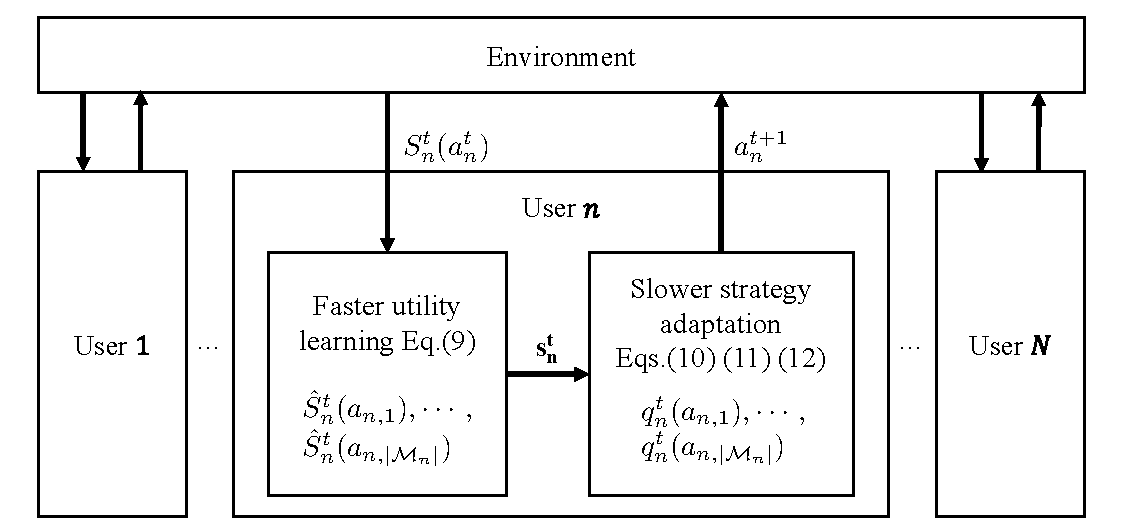
\includegraphics[scale=0.76]{./pic/scheme2.pdf}
%\caption{Illustration of the coupling of utility learning (on faster timescale) and strategy adaptation (on slower timescale) at time $t$.}\label{fg:scheme}
\caption{$t$时刻时效用学习与策略学习之间耦合关系的示意图}\label{fg:scheme}
\end{figure}
我们使用图\ref{fg:scheme}来进一步说明在任意时间步长$t$内效用学习与策略学习之间的耦合。简而言之,在提出的基于遗憾度量的双时间尺度学习算法中,用户在对其长期社交群体效用进行学习的同时,同步地进行策略上的迭代以调整到具有较高“遗憾”度量的信道选择上。在每次迭代中,每个用户都使用其维护的平均遗憾矩阵来计算瞬时遗憾度量(计算复杂度为$O(|\mathcal{M}_n|)$)。接下来,我们对于所提出的学习算法的收敛性能进行评估。
%For clarification, we use Fig. \ref{fg:scheme} to illustrate the coupling of the two learning processes at an arbitrary time step $t$. Simply put, in the proposed regret-based two-timescale learning algorithm, users synchronously learn their long-term group utilities in parallel to the adaptation of their strategies in favor of channels with higher `regret'. At each iteration, each user makes use of her maintained average regret matrix to calculate the instantaneous regret measure, leading to a computational complexity of $O(|\mathcal{M}_n|)$. Next, we evaluate the convergence performance of our proposed learning algorithm.
\vspace{-0.2cm}

\subsection{收敛性分析}\label{sec:conv}

在本节中,我们分析算法\ref{alg:RCS}的收敛性能。我们算法的核心思想是令效用学习和基于无悔学习的策略调整在不同的时间尺度上平行地进行,从而使在较大时间尺度上运行的策略学习可以视在较小时间尺度上运行的效用学习为准静态。我们将采用标准随机逼近理论在双时间尺度上的拓展来证明博弈$\Gamma$对于相关均衡集合的弱收敛性。以下定理给出了我们的主要结果。
%In this section, we analyze the convergence behavior of Algorithm \ref{alg:RCS}. We resort to the two-timescale extension of standard Stochastic approximation theory to show the weakly convergence of game $\Gamma$ to the set of correlated equilibria. The idea is to let the utility learning and regret-based strategy adaptation proceed simultaneously with different step-size schedules so that the regret-based strategy learning runs on a slower effective timescale and sees the utility learning as quasi-static. Our main result is given in the following theorem.
\begin{as}\label{as1}
对于每一个用户$n\in\V$,满足以下条件\textbf{C1-C3},
%For each user $n\in\V$, the conditions \textbf{C1-C3} are satisfied,
\vspace{-0.2cm}
\begin{align}
&\textbf{C1}:\lim_{t\rightarrow\infty}\sum_{t\geq0}\lambda^t_n=+\infty,~\lim_{t\rightarrow\infty}\sum_{t\geq0}(\lambda^t_n)^2<+\infty.\\
&\textbf{C2}:\lim_{t\rightarrow\infty}\sum_{t\geq0}\epsilon^t_n=+\infty,~\lim_{t\rightarrow\infty}\sum_{t\geq0}(\epsilon^t_n)^2<+\infty.\\
&\textbf{C3}:\lim_{t\rightarrow\infty}\frac{\epsilon^t_n}{\lambda^t_n}=0.
\end{align}
\end{as}
\vspace{-0.3cm}
\begin{thm}(算法\ref{alg:RCS}的收敛性)\label{thm:conv}
令$f^t\in\Delta\mathcal{M}$为式(\ref{eq:empi})中定义的经验分布。在满足假设\ref{as1}且式(\ref{eq:reg2})中$\epsilon^t=1/t$的条件下,算法\ref{alg:RCS}收敛到博弈$\Gamma$的相关均衡(CE)的集合$\{\p^*\}$,其中$\pi^*=(\pi^*_1,\pi^*_2,\cdots,\pi^*_N)\in\Delta\mathcal{M}$。特别的,我们有
%Let $f^t\in\Delta\mathcal{M}$ be the empirical distribution as defined in (\ref{eq:empi}). With $\epsilon^t=1/t$ in (\ref{eq:reg2}) and Assumption \ref{as1} being satisfied, Algorithm 1 converges almost surely to the set of CE $\{\p^*\}$ of the game $\Gamma$ with $\pi^*=(\pi^*_1,\pi^*_2,\cdots,\pi^*_N)\in\Delta\mathcal{M}$. In particular, we have,
\begin{align}\label{sne}
&\lim_{t\rightarrow\infty}\hat{S}^t_n(a_{n,i})=\bar{S}_n(a_{n,i},\p^*_{-n}),~\forall n\in\mathcal{M}athcal{V},~\forall i=1,\cdots,|\mathcal{M}_n|,\\
&\mathcal{M}box{and}~~f^t\xrightarrow[\text{}]{\text{a.s.}}\{\pi^*\}~\mathcal{M}box{as}~t\rightarrow\infty.
\end{align}
其中$\bar{S}_n(a_{n,i},\p^*_{-n})$是当用户$n$选择决策$a_{n,i}$,其他用户联合策略为$\pi^*_{-n}$时的期望社交群体效用。
%where $\bar{S}_n(a_{n,i},\p^*_{-n})$ is the expected group utility of user $n$ with action $a_{n,i}$ and others' strategies $\pi^*_{-n}$.
\end{thm}

%\textbf{Outline of the proof.}
定理证明的主要思想是首先引入离散学习过程(\ref{estimation})和(\ref{eq:reg2})的连续时间插值过程。首先,每个学习过程在数学上分别对应于一个微分包含(differential inclusion)\cite{Yin}。而其连续时间差值过程可被证明为对应的微分包含的半流渐近伪轨迹(asymptotic pseudotrajectory of the semiflow)。因而,我们可以通过微分包含来研究序列$\{S_n(\A)\}$和$\{\pi(\A)\}$的极限行为。在满足假设\ref{as1}的前提下,通过结合异步随机逼近框架\cite{Borkar1997},我们可以获得两个并行的学习过程的渐近弱收敛结果。由于篇幅所限,我们在线附录\ref{pf:thm:conv}部分提供详细的证明。
%The main idea of the proof is to first introduce the continuous time interpolated process of the discrete learning process (\ref{estimation}) and (\ref{eq:reg2}), which can be shown to be the asymptotic pseudotrajectory of the semiflow corresponding to the differential inclusion defined by the two learning dynamics\cite{Yin}. Thus the limiting behaviors of the sequences $\{S_n(\A)\}$ and $\{\pi(\A)\}$ can be studied via the differential inclusion. By combining the asynchronous stochastic approximation framework \cite{Borkar1997}, and under the Assumption \ref{as1}, we can obtain the asymptotic weak convergence result of the two concurrent learning processes. Due to the lack of space, we leave the detailed proof to the online appendix \cite{MY18}.

%\vspace{-0.2cm}
\section{性能评估}\label{sec:simulation}
在本节中,我们评估了用于隐私保护下频谱共享的双时间尺度分布式学习算法的性能。
%In this section, we evaluate the performance of the proposed two-timescale distributed learning algorithm for the privacy-preserving spectrum sharing.
%\vspace{-0.4cm}
\subsection{仿真设置}
我们考虑一个数据库辅助的频谱接入网络,该网络由$N=80$个次级用户组成,我们假设这些用户随机分布在$1km \times 1km$的正方形地理区域中。每个用户$n$对应于一个有数据发送需求的移动设备,其默认传输功率为$P_n=100$ mW\cite{FCCApril52012}。我们假设每个用户的可用信道集合即为总的可用信道集合,即$\mathcal{M}_n=\mathcal{M}athcal{A}$,并设置默认的信道总数为$M=5$。我们考虑瑞利信道衰落模型,其中用户$n$和$m$之间的信道增益反比于他们之间的物理距离(路径损耗因子$\alpha = 4$)。我们令$N_{a_n}$表示用户$n$使用信道$a_n$时的背景干扰功率,并假设其数值服从区间[-100,-90] dBm上的均匀分布。我们假设所有的用户被随机分到两个社交群体中,每个群体中用户$n$的权重因子$e_{n}$从均匀分布$\mathcal{M}athcal{U}(e_{min},1)$采样获得,并且设置$e_{min}$的默认值为0.5。
%We consider a database-assisted spectrum access network consisting of $N=80$ IoT devices that are randomly scattered in a square area of 1 km $\times$ 1 km and are categorized into either one of two groups with equal probability. For each secondary user $n$, we set the transmission power before being perturbed as $P_n=100$ mW \cite{FCC} and the available channel set $\mathcal{M}_n=\mathcal{M}athcal{A}$ with $M=5$ by default. We consider a Rayleigh fading channel environment where the channel gain between user $n$ and $m$ is inversely proportional to their physical distance powered by the path-loss factor $\alpha=4$. The background interference power $N_{a_n}$ for each user $n$ using channel $a_n$ is uniformly assigned in the interval of [-100,-90] dBm. The weight factor $e_{n}$ for each user $n$ in either group is generated following a uniform distribution $\mathcal{M}athcal{U}(e_{min},1)$ with $e_{min}=0.5$ by default.
如节\ref{sec:privacy-model}中所述,我们的设计中每个用户通过对其传输功率进行随机扰动以对抗基于RSS的定位攻击。功率扰动程度越大,对于攻击者定位准确性的影响越显著,继而对于位置隐私的保护作用越好。在实验中,我们使用功率扰动的期望值$E(\Delta p_n)$来量化隐私保护程度的大小。
根据式(\ref{eq:noise}),我们可以得出功率扰动项的期望值的表达式为$E(\Delta p_n)=b\left[\frac{1-(k+1)\exp(-k)}{1-\exp(-k)}\right]$,其中$k=\bar{p}/b>0$。我们固定$\bar{p}=15$ mW并默认设置$b=12$,以使平均功率扰动水平约为-6mW。
对于前文提出的双时间尺度学习算法\ref{alg:RCS},我们分别设置学习率为$\lambda^t=t^{-0.5}$和$\epsilon^t=t^{-0.2}$。在满足条件\textbf{C1-C3}的前提下,我们通过网格搜索确定超参数的取值。对于参数$\rho$,我们使用与文献\cite{Hart_areinforcement}中同样的设置,即$\rho=1/8$。
%In our experiment, we let each user randomly perturb her transmission power level to combat the RSS based localization attack (as introduced in Section \ref{sec:privacy-model}), where each user's privacy protection level is quantified by the expected value of power perturbation $E(\Delta p_n)$. According to (\ref{eq:noise}), we can derive the expression for the expected value of power perturbation term as $E(\Delta p_n)=b\left[\frac{1-(k+1)\exp(-k)}{1-\exp(-k)}\right]$, where $k=\bar{p}/b>0$. We fix $\bar{p}=15$mW and set $b=12$ by default such that the mean perturbation level is about -6mW.
%For the two-timescale learning algorithm, we set the learning rate $\lambda^t=t^{-0.5}$ and $\epsilon^t=t^{-0.2}$ in Algorithm 1. The value of hyperparameters are determined through a tuning process so that the conditions \textbf{C1-C3} are satisfied. In addition, we let $\rho=1/8$ as it is used in \cite{Hart_areinforcement}. 

%\vspace{-0.2cm}
\subsection{结果与讨论}
\subsubsection{收敛表现}
我们首先检查算法的收敛性能。在默认设置$E(\Delta p_n)=-6$ mW,$e_{min}=0.5$的条件下,我们针对不同数量的可用信道集合进行实验,即$M=4,5,6$。我们使用网络吞吐量$T=\frac{1}{N}\sum_{n\in\mathcal{M}athcal{V}}T_n$作为性能指标,其中$T_n$表示用户$n$的平均吞吐量。从图\ref{fg:conv1}中我们观察到算法在1500次迭代内可以收敛,而通道总数的增加会导致收敛时间的增长。同时可以看出,系统可实现的最大网络吞吐量大约占网络吞吐量最优值的90%,且并不会受到信道集合大小变化的影响。图\ref{fg:conv2}则分别展示了任意选择的一个用户(\#10)所对应的每一个信道的策略的收敛性表现。
%We first examine the convergence performance of our algorithm. We adjust the value of $b$ so that the mean value of power perturbation magnitude is -5 mW and the minimum group-relationship strength $e_{min}=0.5$. We first run the experiment with different number of available channels, $M=4,5,6$. The network throughput $T=\frac{1}{N}\sum_{n\in\mathcal{M}athcal{V}} T_n$ is used as the performance metric, where $T_n$ denotes the average throughput of user $n$. From Fig. \ref{fg:conv1}, we observe that the proposed algorithm converges within 1500 iterations in general with increased number of channels leading to longer convergence time. It can be observed that changing the size of channel set does not impact the maximum achievable network throughput, which accounts for about 90\% of the optimal network throughput. For an arbitrary selected user \#10, we further evaluate the convergence of her strategies over each of the available channels, as shown in Fig. \ref{fg:conv2}.
%\begin{figure}[htb]
%\centering
%\subfloat[]{
%	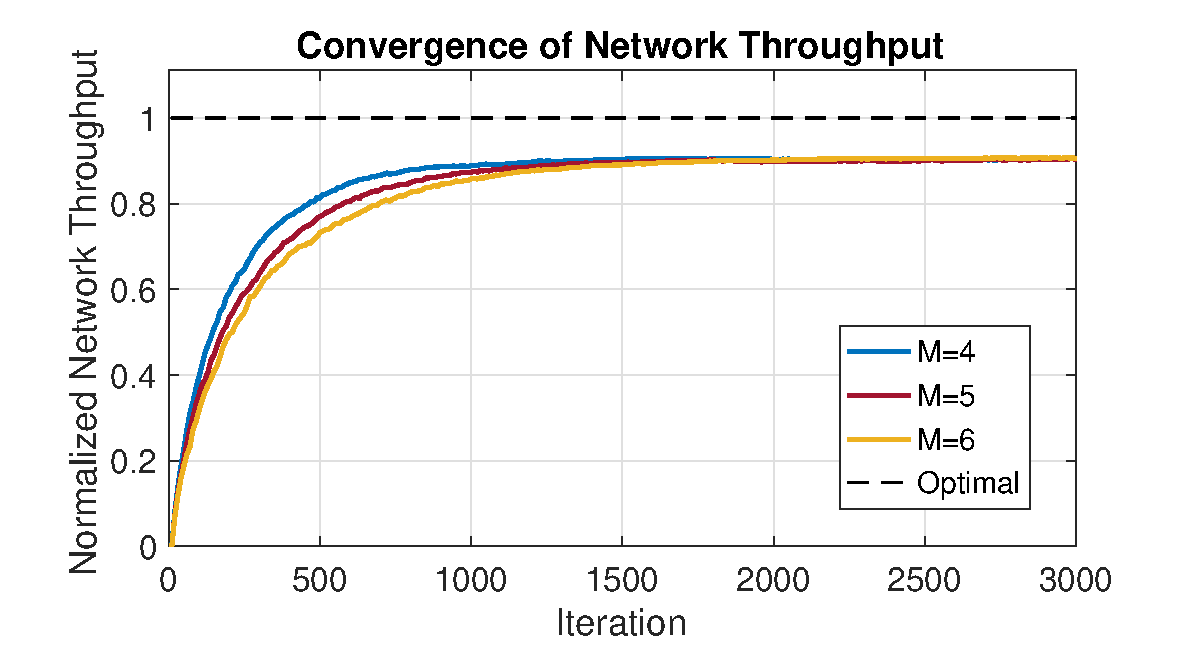
\includegraphics[scale=0.41]{./pic/conv_ch3.eps}\label{fg:conv1}}
%\vfill
%%\vspace{-0.3cm}
%\centering
%\subfloat[]{
%	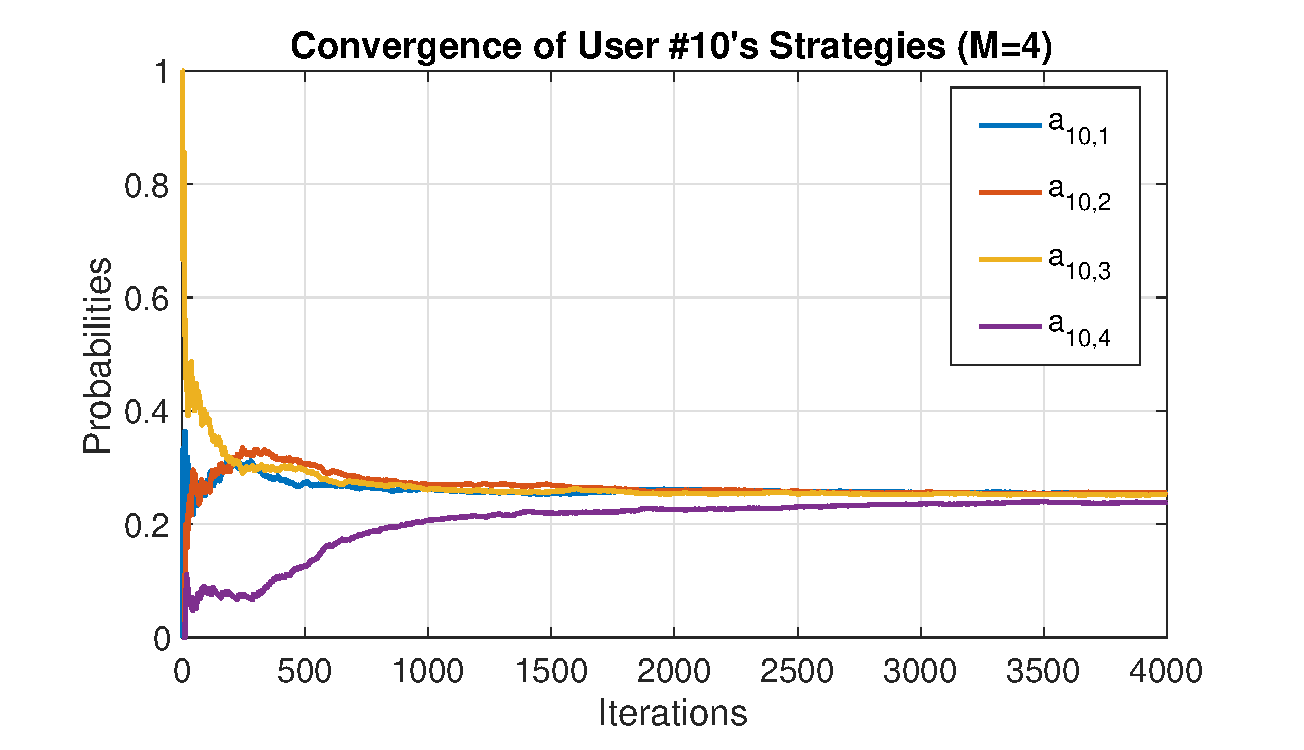
\includegraphics[scale=0.4]{./pic/str_conv4.eps}\label{fg:conv2}}
%%\hfill
%\caption{Convergence performance of two-timescale distributed learning algorithm.}\label{fg:Fig11}
%\end{figure}

%\begin{figure*}[!t]
%	\begin{minipage}[t]{0.48\textwidth}
%		\centering
%		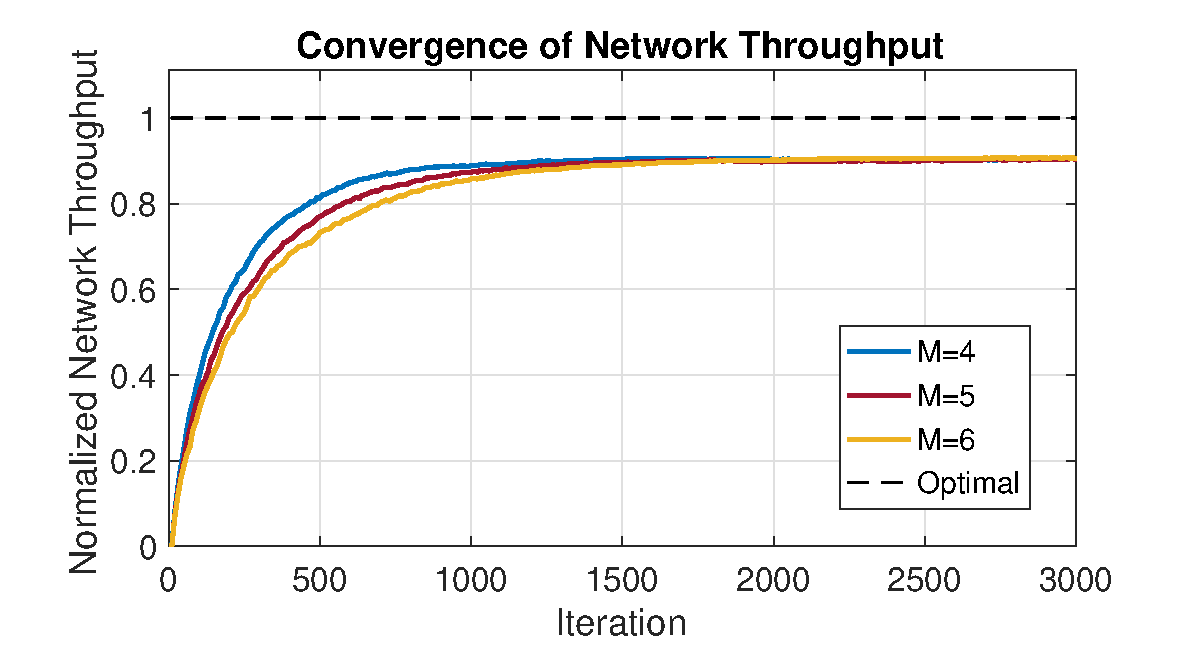
\includegraphics[scale=0.44]{./pic/conv_ch3.eps}
%		\caption{网络吞吐量的收敛表现}\label{fg:conv1}
%	\end{minipage}
%	\hfill
%	\begin{minipage}[t]{0.48\textwidth}
%		\centering
%		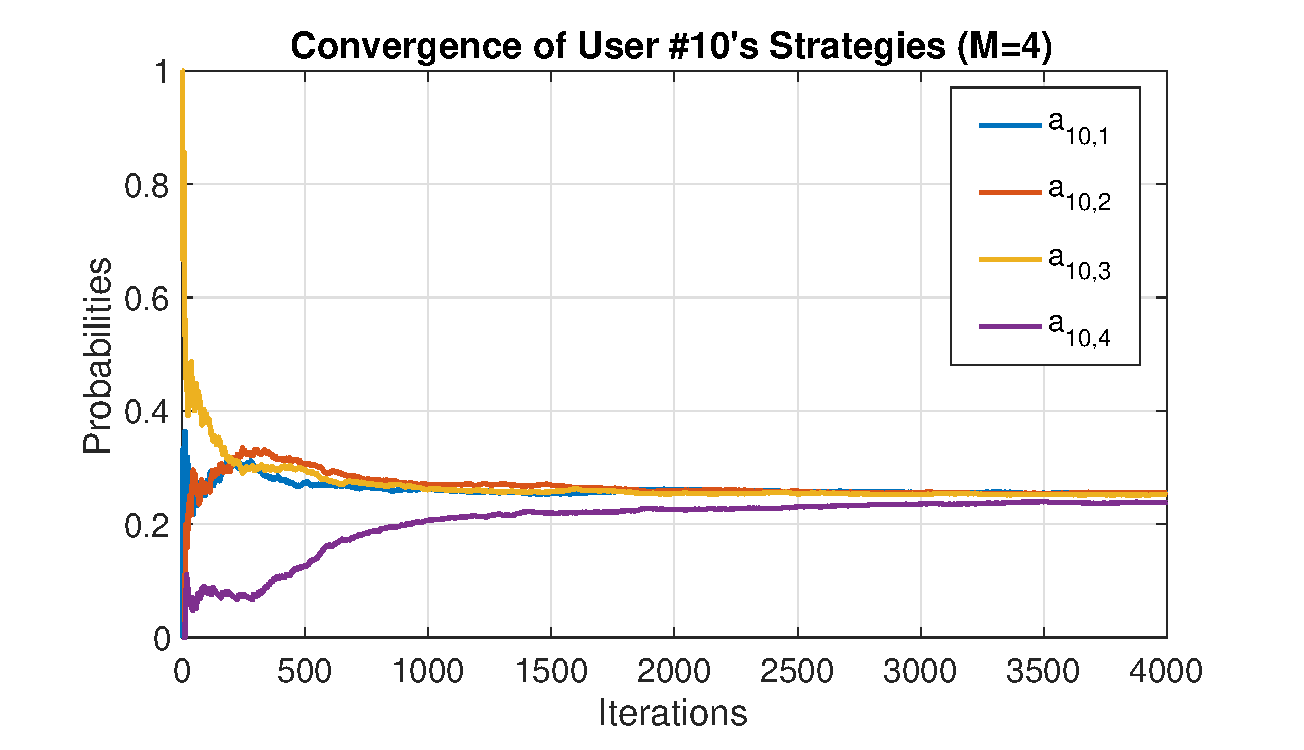
\includegraphics[scale=0.42]{./pic/str_conv4.eps}
%		\caption{用户\#10的策略收敛表现 (M=4)}\label{fg:conv2}
%	\end{minipage}
%	\caption{双时间尺度分布式学习算法的收敛性表现}
%	\label{fg:Fig11}
%\end{figure*}

\begin{figure*}[!t]
%	\begin{minipage}[t]{0.48\textwidth}
		\centering
		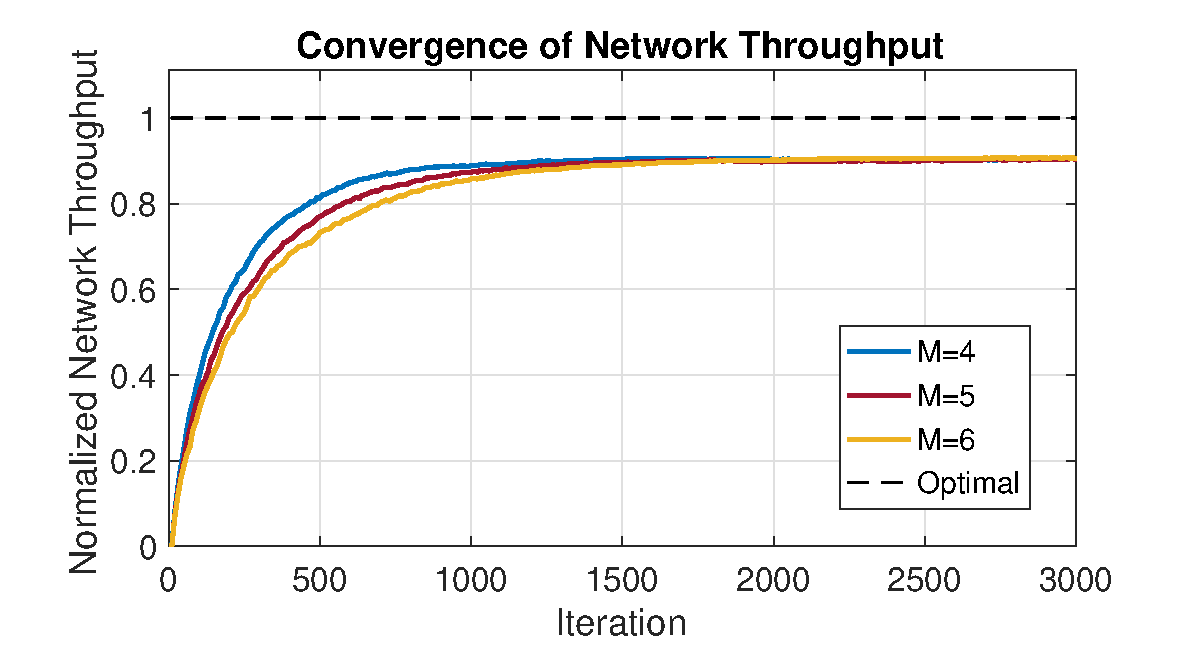
\includegraphics[scale=0.65]{./pic/conv_ch3.eps}
		\caption{网络吞吐量的收敛表现}\label{fg:conv1}
\end{figure*}
%	\end{minipage}
%	\hfill
%	\begin{minipage}[t]{0.48\textwidth}
\begin{figure*}[!t]
		\centering
		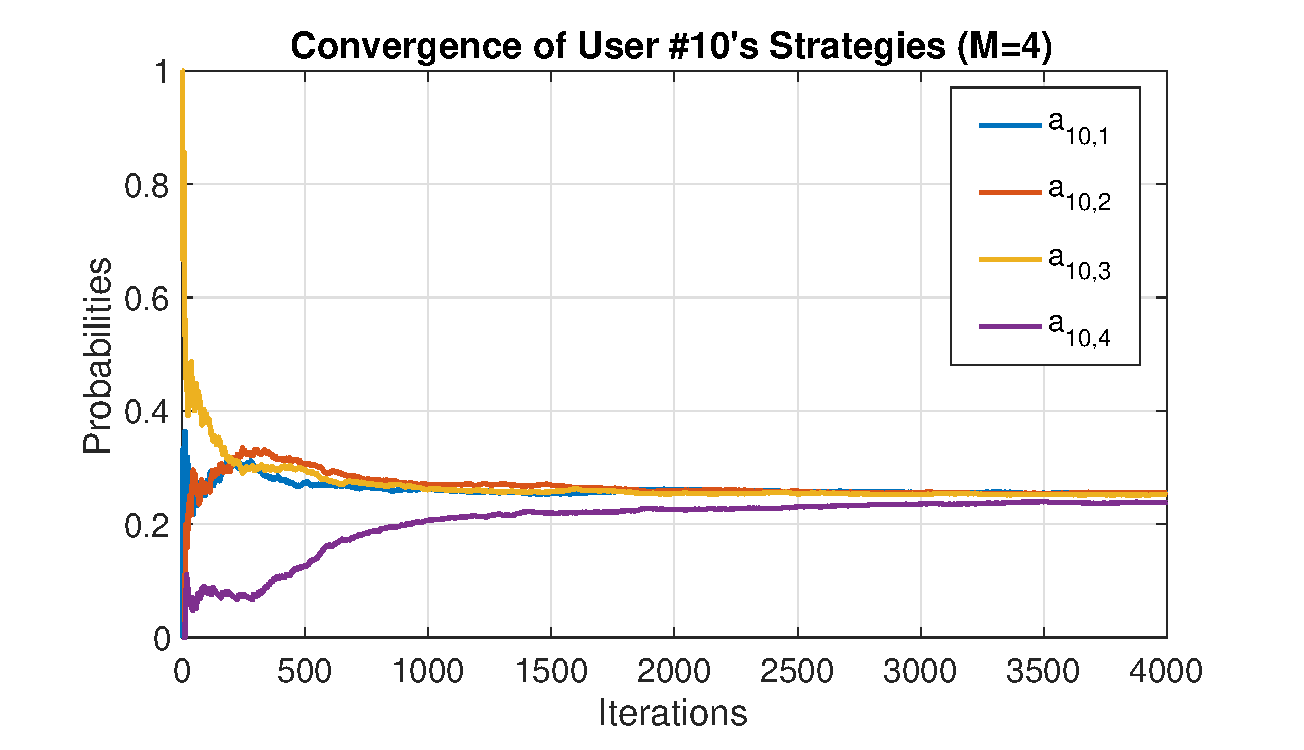
\includegraphics[scale=0.64]{./pic/str_conv4.eps}
		\caption{用户\#10的策略收敛表现 (M=4)}\label{fg:conv2}
%	\end{minipage}
%	\caption{双时间尺度分布式学习算法的收敛性表现}
%	\label{fg:Fig11}
\end{figure*}



\subsubsection{关于吞吐量-隐私权衡的比较性实验}
%\subsubsection{Comparative studies on the throughput-privacy tradeoff}
我们接下来研究在不同功率扰动水平下网络吞吐量与位置隐私之间的权衡。我们使用默认设置$M = 5$,$e_ {min} = 0.5$,并在不同功率扰动级别下运行实验。具体来说,我们通过更改参数$b$的值,使得扰动功率的平均值在0mW至-9mW之间变化。为了进行比较研究,我们考虑了两个基准:(a)单一时间尺度学习算法,该算法仅使用\ref{sec:single}节中所介绍的修正后的无悔学习规则进行策略上的调整而不引入对于效用的学习; (b)双时间尺度学习算法,其中包括在较小时间尺度上对于效用的学习以及在较大时间尺度上使用随机虚拟对弈(Stochastic Fictitious Play)\cite{ZhangGlobe}进行策略调整。

%We next investigate the tradeoffs between network throughput and location privacy under different levels of power perturbation. We use the default setting of $M=5$, $e_{min}=0.5$, and run the experiment under different levels of power perturbation. Specifically, we change the value of parameter $b$ so that the mean value of perturbation power level varies from 0mW to -9mW. For the comparative study, we consider two benchmarks: (a) the single timescale learning algorithm that merely consists of strategy adaptation based on modified regret based learning (RBL) as introduced in Section \ref{sec:single}; (b) the two-timescale learning algorithm involving a utility learning as well as a strategy adaptation following the Stochastic Fictitious Play (SFP) \cite{ZhangGlobe}. 

如图\ref{fg:Fig33}所示,正如所预期的,系统吞吐量会随平均功率扰动水平的增加而降低。同时,很明显,使用单一时间尺度的学习算法在隐私保护级别升高时,网络吞吐量较其他两种算法相比下降得更快。这表明引入平行的效用学习来校准带有噪声的效用观测值的有效性。这也有助于我们可以在位置隐私保护与保证网络性能(即系统吞吐量)之间取得权衡。
%As shown in Fig. \ref{fg:Fig33}, in general, the system throughput decreases as expected with the increase of mean power perturbation level. Meanwhile, it is clear that the throughput of single timescale learning using RBL degrades much faster as the privacy preserving level increases, compared with other two approaches that involve both utility learning and strategy adaptation. This indicates the effectiveness of using a parallel utility learning to calibrate the noisy utility observation, which helps balance the location privacy protection with the network performance (i.e., system throughput). 

从图\ref{fg:Fig33}中还可以看出,我们所提出的基于无悔学习的双时间尺度算法所获得的平均吞吐量比使用\cite{ZhangGlobe}中提出的双时间尺度学习方法所获得的平均吞吐量平均要高5%。这样的结果可以由两种方案中所使用的不同均衡标准来解释。文献\cite{ZhangGlobe}中提出的算法针对的是纳什均衡。根据定义,纳什均衡假设博弈参与者的策略之间是相互独立的,而本研究中所考虑的相关均衡则允许参与者的策略之间存在相关性,因此相比纳什均衡更具一般性。由于相关平衡的集合在数学上等价于一个凸多胞形,并且凸多胞形的每一个极值点即对应于一个纳什均衡点,因此一般而言以相关均衡为考虑对象可以使得结果展现出更好的性能。
%It can also be seen that the throughput obtained by our proposed algorithm outweighs the one obtained using the two-timescale learning approach introduced in \cite{ZhangGlobe} by 5\% in average. This can be explained by the different  Equilibrium criteria used in the two studies. By definition, Nash equilibrium uses an underlying assumption that players' strategies are mutually independent. While the correlated equilibrium considered in this study generalizes the Nash equilibrium by allowing the strategies to be dependent among players. As the correlated equilibrium is mathematically equivalent to a convex polytope with its extrema points corresponding to the set of Nash equilibria, it is likely to exhibits better performance in general. 
\begin{figure}[htb]
\centering
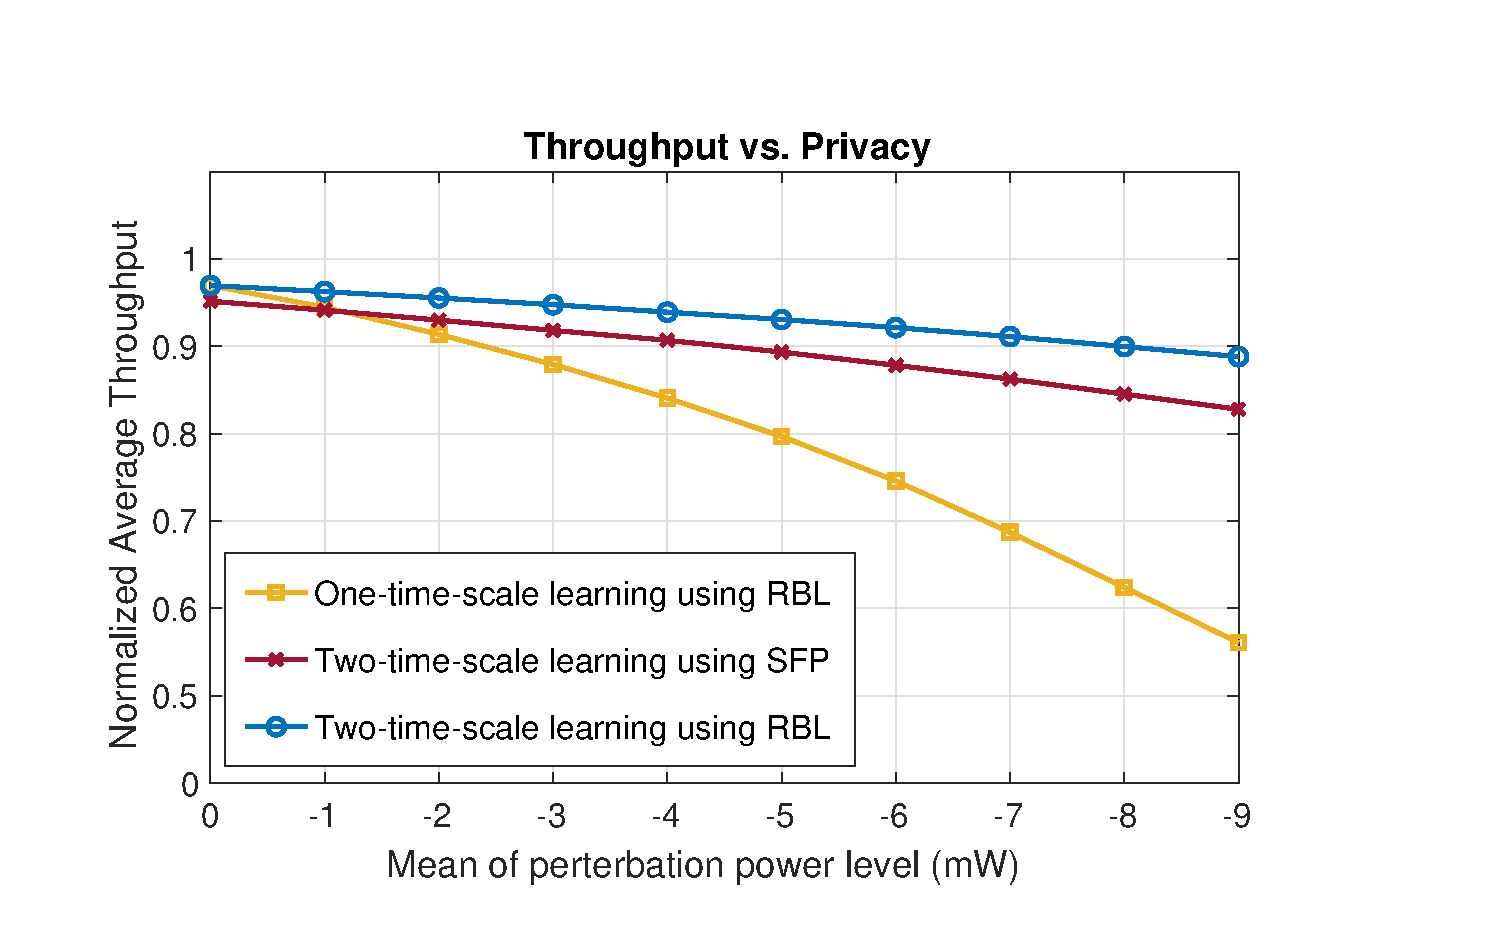
\includegraphics[scale=0.58]{./pic/thp_pert_new3.eps}
%\vspace{-0.0cm}
%\caption{Performance comparisons among different learning algorithms under varying power perturbation level.}
\caption{几种学习算法在不同功率扰动水平下的性能比较}\label{fg:Fig33}
\end{figure}
%\vspace{-0.2cm}
\begin{figure}[htb]
\centering
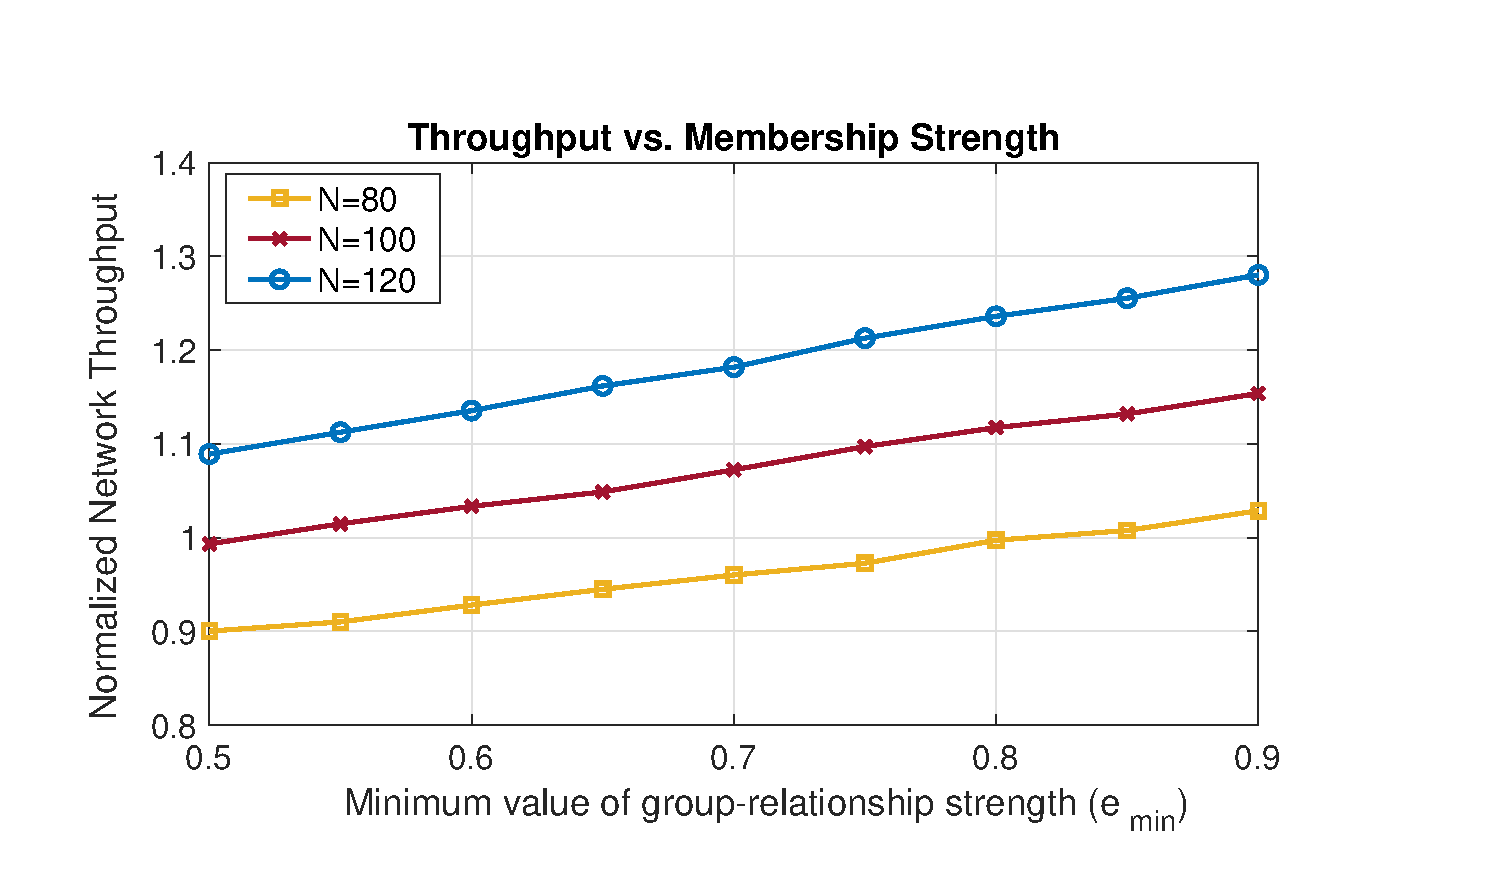
\includegraphics[scale=0.58]{./pic/thp_soc_new3.eps}
%\vspace{-0.3cm}
\caption{社交联系强度对吞吐量的影响}\label{fg:Fig22}
\end{figure}
\subsubsection{网络外部性对于系统吞吐量的影响} 我们最后对网络外部性对系统性能的影响进行评估。实验中我们分别针对三种网络规模(即$N = 80, 100, 120$)在将社交关联强度参数$e_ {min}$取值从0.5增加到0.9的过程中对系统的吞吐量进行了考察。如图\ref{fg:Fig22}所示,随着系统规模的扩大,网络吞吐量呈逐步增长的趋势。另外,可以看出,系统吞吐量会随着社交关联强度的增加而单调增加。具体的,对于$N = 80, 100, 120$的三种情况,当$e_ {min}$从0.5增加到0.9时,系统性能分别可以获得大约14.5%,15%和16.4%的提升。这说明正向的网络外部性影响有助于提升系统的表明。
%We finally examine the network impact to the system performance. We run the experiment with increasing $e_{min}$ from 0.5 to 0.9 for three cases with different network scale, i.e., $N=80, 100, 120$. As illustrated in Fig. \ref{fg:Fig22}, the network throughput grows in general as the system scale enlarges. Also, it can be seen that the throughput experiences a monotonically increase as the strength of in-group relationship increases. For the cases with $N=80, 100, 120$, approximately 14.5\%, 15\%, and 16.4\% performance gains are achieved, respectively, when $e_{min}$ is increased from 0.5 to 0.9, which indicates that the system would benefit from users behaving more altruistically. 

%\vspace{-0.2cm}
\section{本章小节}\label{sec:con}
本章关注了认知无线电网络中的数据库辅助频谱共享技术,其中次级用户在双重网络外部性的作用下分别在社交域和物理域中都存在相互耦合。针对潜在的基于RSS的位置隐私攻击,次级用户使用随机功率扰动的方法来降低攻击者的定位精度。本文将隐私保护下具有社会意识的频谱共享建模为次级用户之间的随机信道选择博弈。基于无悔学习的规则,本文设计了一种双时间尺度的分布式学习算法。算法中,每个用户持续对自己带有噪声的期望社交团体效用进行估计,并根据降低遗憾度量的目标调整其信道选择策略。本文所提出的算法具有针对相关均衡集合的弱收敛性。数值结果证实较高的隐私保护级别将导致更严重的网络吞吐量下降。
%In this paper, we studied database assisted spectrum sharing where secondary users are coupled both in the social domain and in the physical domain. To address the RSS-based location privacy attack, a random power perturbation approach is applied to reduce the localization accuracy. We cast the socially-aware privacy-preserving spectrum sharing as a stochastic channel selection game among secondary users. Based on no regret dynamics, we develop a two-time-scale distributed learning algorithm in which each user continuously estimates her social group utility and adapts her strategy in favor of reduced regrets. Our algorithm is shown to weakly converge towards the set of correlated equilibrium. The numerical results corroborate that higher privacy protection level would lead to severer network throughput degradation.



%\chapter{毫米波蜂窝系统基站天线资源分配与优化研究}

\textbf{本章摘要:} 
Mobile crowdsensing (MCS) is an emerging technology that exploits the enormous sensing power of widely used mobile devices to complete sensing tasks in a cost-efficient manner. Among all outstanding issues of current MCS systems, the concern of lacking privacy protection for the sensing data of participants has drawn increasing attention recently. Various privacy-preserving MCS mechanisms have been proposed for the static scenario where users' privacy protection requirements remain unchanged. In practice, however, users' requirements for privacy protection can be time-varying, which further complicates the design of privacy-preserving MCS. In this article, we first give an overview of multiple promising approaches for privacy-preserving MCS, based on which we make a first attempt to explore the privacy-preserving MCS in a dynamic scenario, which is cast as a Markov Decision Process. Specifically, we develop a reinforcement learning based approach, by which the platform can dynamically adapt its pricing policy catering to the varying privacy-preserving levels of participating users. We further use a case study to evaluate the performance of our proposed approach.

\textbf{关键词:}频谱接入;ICPS安全;分布式算法;博弈论
%\keywords{毫米波通信;Massive MIMO;整数规划}

\section{引言}
Recently, mobile crowdsensing (MCS) has emerged as a popular and effective approach for various sensing tasks (e.g., air quality monitoring, civil noise level measurement, and traffic congestion monitoring \cite{waze, hu2015smartroad, cheng2014aircloud}). In the spirit of crowdsourcing, MCS outsources a collection of sensing tasks to human-carried smart devices equipped with various sensors (e.g., camera, micro-phone, GPS, gyroscope, and accelerometer). Compared with conventional sensor networks, MCS can collect fine-grained information in a more flexible and cost-efficient manner. 

Sensing data contributed by mobile users may contain users' sensitive (private) information, thereby giving rise to privacy concerns when being released to an untrusted party. This becomes a key challenge of designing a MCS system, i.e., how to design efficient incentive mechanisms to stimulate users' participation while preserving user privacy. Traditionally, extensive studies have employed economic approaches to design incentive schemes to attract mobile users' participation, such as auction, game theory, and contract theory \cite{jin2016, zhang2016privacy, wang2016value}. One common assumption made in these works is that system parameters such as sensing utility and mobile users' profiles do not change with time. 

Recently, unified crowdsensing platform design has drawn much attention. In such a platform, participated users can simultaneously fulfill multiple complex sensing tasks for different applications, possibly across a long time period. It is possible that users have different privacy protection requirements when completing different sensing tasks. For example, a user may have higher privacy-preserving level when performing a sensing task for medical applications, in contrast to a lower privacy-preserving level for location based applications. Further, their privacy-preserving levels may change over time (e.g., people may raise the privacy-preserving levels for medical applications when they get sick). This calls for a new approach for such dynamic scenarios where the system parameters are time-varying. 

In this article, we first present an overview of existing incentive mechanisms for MCS that designed to meet static privacy protection requirements. We then focus on the dynamic scenario where each participated user is empowered to locally perturb her sensing data according to a self-specified and time-variant privacy-preserving level. Without knowing users' payoff functions and the changing dynamics of their privacy-preserving levels, it is challenging for the platform to determine the pricing policy via offline approaches. To this end, we propose a learning based approach to adaptively adjust the pricing for sensing tasks while preserving mobile users' privacy. Specifically, the MCS system is modeled as a Markov Decision Process, where each state corresponds to the current privacy-preserving levels of all users. Based on the the observed system state and the perceived reward, the platform adapts its pricing policy dynamically to optimize its utility using a Q-learning based algorithm\cite{Sutton98a}. Intuitively, more payment would be awarded to users with low privacy-preserving levels in order to encourage the contribution of high-quality data. Notably, compared with existing solutions, our proposed learning based pricing mechanism does not require any knowledge about mobile users' payoff function, and enables users to autonomously specify their privacy-preserving requirements under different situations. 

The remainder of this article is organized as follows: In Section \ref{sec:s2}, we review a data privacy attack model as well as two effective data perturbation methods. In Section \ref{sec:s3}, we provide an overview of the existing designs that have integrated the data privacy protection with incentive mechanism. Next, in Section \ref{sec:s4}, we study the MCS scenario where users' privacy-preserving requirements are time-varying and propose a Q-learning based dynamic pricing mechanism. Finally, Section \ref{sec:s5} concludes this article.

\section{研究现状Data Privacy in MCS}\label{sec:s2}
In this article, we consider a semi-trustworthy platform, who collects the sensing data provided by the mobile users. In the following, we first introduce the Bayesian attack model that aims to infer users' sensitive sensing data. Then, we introduce the differential privacy mechanism that can effectively combat the Bayesian privacy attack in MCS.

\subsection{Bayesian Privacy Attack Model}
We assume that a mobile user has private sensing data $x\in\ca{X}$ with $\ca{X}$ denoting the domain of the data value. We also assume that an adversary has the \emph{prior} knowledge about the probabilistic distribution $\pi(x)$ of a participated user's sensing result $x\in\ca{X}$, as well as the probability $p(x^*|x)$ under which a sensing data $x\in\ca{X}$ is obfuscated to $x^*\in\ca{X}$. Then, with the observation of $x^*$, the attacker can derive a \emph{posterior} distribution of user's true sensing result, $p(x|x^*)$, based on Bayes' rule\cite{Leye}:
\begin{equation}
p(x|x^*)=\frac{p(x^*|x)\cdot\pi(x)}{\sum_{x'\in\ca{X}}p(x^*|x')\cdot\pi(x')}.
\end{equation}
In order to combat this Bayesian privacy attack, we design a privacy-preserving mechanism that can bound the improvement of the attacker's \emph{posterior} knowledge over her \emph{prior} knowledge. In other words, it is desirable to have the value of $p(x^*|x)$ and $p(x^*|x')$ close enough so that, given the observation $x^*$, the attacker can hardly distinguish $x$ and $x'$. To this end, we resort to the celebrated notion of differential privacy.

\subsection{Data Differential Privacy}
Following \cite{wang2016value}, we define the differential privacy-preserving level of a user as follows.

\begin{df}[Differential-Privacy-Preserving Level]\label{def1}
The differential privacy-preserving level (DPL) of a user, denoted by $\epsilon$, is defined as
\begin{equation}
\epsilon = \max\left\{\ln\left(\frac{p(x^*|x)}{p(x^*|x')}\right)\right\}, ~\forall x, x'\in\ca{X}.
\end{equation}
\end{df}
A user's $DPL$ quantifies the potential leakage of privacy under the \emph{prior} knowledge of attacker by measuring the indistinguishability between the conditional probability of the reported data. It can be easily proved that with $DPL=\epsilon$, the knowledge gain of an attacker, $g=p(x|x^*)/p(x)$, is bounded as $1/e^\epsilon\leq g\leq e^\epsilon$ with \emph{prior} knowledge $p(x)$. Clearly, the smaller the $\epsilon$, the harder for the attacker to correctly infer out the true data, and hence the better the privacy-preserving performance. We next review two local data perturbation methods, by which a certain differential privacy-preserving level for a user's data can be achieved.

\textbf{Laplace mechanism.}
Laplace mechanism is a widely used technique that provides differential privacy gurantees\cite{dwork2014algorithmic}. In this paper, we are interested especially in a variant version of Laplace mechanism, in which a Laplacian noise $\eta\sim Lap(\Delta/\epsilon)$ is added locally to each individual user's data where $\Delta \triangleq \max_{x,x'\in\ca{X}}|x-x'|$ is defined as the local sensitivity and $\epsilon$ is the $DPL$ of that user.  

\textbf{Randomized response.}
Randomized response is another tool that can provide local differential privacy guarantees\cite{dwork2014algorithmic}. With certain probability, the individual user sends a random instance of her real data to the untrusted data collector. The parameters of randomized response mechanism are carefully chosen to limit the platform's ability to learn with confidence about the true value of the data. %As an illustrating example, when the data is one bit binary data, the data owner can flip a biased coin, and report the truth to the platform if the coin comes up head, and tell the opposite answer if it comes up tail. The data owner thus preserves the data privacy due to the coin randomness.

\section{Noise Injection based Privacy-preserving Approaches in MCS}\label{sec:s3}
In this section, we give an overview of several state-of-art privacy-preserving MCS designs that integrate differential-private noise injection with incentive mechanism design. We classify these works according to the types of incentive mechanisms they used, which includes \emph{auction} based approach, \emph{game theory} based approach, and \emph{contract theory} based approach.



\subsection{Auction based Approach}
The (reverse) auction mechanism is one of the most popular approaches for platform-centric MCS incentive mechanism design. In specific, the platform acts as the auctioneer and the mobile users report their bids reflecting their participation costs to the platform. The platform selects the participants and determines the corresponding payments, aiming to minimize the total payment or to maximize the platform utility under the budget constraint, or to maximize the participants' social welfare\cite{DejunJ}. 

In the seminar work by Ghosh and Roth \cite{ghosh2015selling}, an auction mechanism was proposed, where the private data is treated as goods procured by a data analyzer running a survey. Each individual's privacy cost is modeled as a linear function of her differential-privacy-preserving level $\epsilon$. The designed auction mechanism satisfies two fundamental requirements for incentive mechanism design, i.e., truthfulness and individual rationality:
\begin{itemize}
\item Truthfulness: A participated user cannot benefit from bidding untruthfully.
\item Individual Rationality: Each participated user receives a payment that is larger than or equal to her privacy cost.
\end{itemize}
This work\cite{ghosh2015selling} characterizes the tradeoff between the total payment and the result accuracy from the following two perspectives: 1) to minimize the total payment given an accuracy requirement, or 2) to maximize the result accuracy under a payment budget. 

Along this line, Jin \textsl{et al.} developed a combinatorial auction based framework for preserving data privacy in MCS \cite{jin2016}. Specifically, the privacy cost is modeled as part of each user's sensing cost. In addition, the reliability of mobile users, which influences the accuracy of aggregated sensing results, is further considered during the user selection. Related works \cite{zhang2016privacy} considered a setting where the mobile users are embedded in a social network. Worth noting is that both assumed a trusted data collector in their models.

% In addition, they also considered the case of real-time data aggregation in which their proposed mechanism provides long-term incentives aiming to maintain continuous participation. 
%Although the above mentioned works posses some differences in the models they used, all of them apply the Laplacian mechanism for data perturbation. 

\subsection{Game Theory based Approach}
The game theoretic model is another popular approach for incentive mechanism design \cite{DejunJ, he2017exchange,Yang17}. 
%As a user-centric approach, game theory based approach enables mobile users more involvements into the payment determination process. 
Similar to the auction based mechanism design, game-theoretic approaches need to specify a payment policy that incentives users' participation. However, in game based approaches, the participated users are not selected by the platform; instead, given the payment policy of the platform, users make strategic participation decisions. 

Wang \textsl{et al.} in \cite{wang2016value} devised a game-theoretic mechanism in a setting where a data collector purchases users' private data which represents their knowledge about an underlying system state. Different from \cite{ghosh2015selling,jin2016,zhang2016privacy} where a trusted platform carries out centralized data perturbation over aggregated data, an underlying assumption in \cite{wang2016value} is that the data collector is not trustworthy, in which case each participated user is allowed to locally perturb her raw data strategically before releasing it to the data collector. In their game theoretic model, individual users are the players of the game whose actions correspond to their data perturbation strategies. And the pricing strategy is carefully designed by the data collector, so that a Nash equilibrium of the game can be achieved with participated users' privacy cost being compensated and the accuracy requirement of the collected data being satisfied.

\subsection{Contract based Approach}
In a contract-based mechanism, the contract designer would sophistically design a menu of effort-payment pairs to incentivize the participation of individuals with different types, while at the same time optimize its own payoff. Instead of requiring real-time bid information, contract-based approach exploits the statistical information of individuals' costs to determine payment contracts, which overcomes the information asymmetry and reduces communication and computation overhead. In \cite{Kun1}, a contract-based privacy-preserving MCS framework was proposed. Specifically, the platform designs and broadcasts a menu of contracts, each of which specifies one type of differential-privacy-preserving level and the corresponding payment that a user will receive if she agrees with that contract. Each user then chooses one of the contracts that maximizes her utility. The authors derived the quantitative relationship between individual privacy and aggregation accuracy with proper metrics. 

The three approaches reviewed above are summarized in Table 1. Although they applied different mechanism design approaches, their is one common thread: the $DPL$ of each individual user remains unchanged throughout the crowdsensing procedure. In the next section, we extend the current scenario to a more general one, in which case the mobile users' $DPL$s are not static and the platform needs to dynamically adjust the pricing policy to optiize the operation of the MCS system.

\begin{table*}[!htp]
	\caption{Summary of existing data privacy-preserving approaches for mobile crowdsensing}
	\centering
	\tabcolsep=10pt
	\begin{tabular}[c]{|c|c|c|c|c|c|c|c|}
		\hline \label{table:comparison}
		Reference & Mechanism Type & Platform Trusted &  Data Perturbation & $DPL$ & Features \\ \hline\hline
		
		\cite{jin2016}	  & Auction  	   &        Yes		  &	Laplace mechanism	&  Static & Consider users' reliability	\\ \hline

%		\cite{Kun1}	  & Auction	       &        No  	  & Laplace mechanism & Provide long-term incentive mechanism 	\\ \hline
		
		\cite{zhang2016privacy}	  & Auction		   &        Yes 	      & Laplace mechanism  &  Static & Consider social relationship among users	\\ \hline

		\cite{wang2016value}	  & Game		   &        No 	      &   Randomized response	& Static & Analyze users' equilibrium behaviors	\\ \hline

		\cite{Kun1}	  & Contract	   &		No		  & Laplace mechanism & Static & Overcome information asymmetry \\ \hline

		This paper & -- &		No		  & Laplace mechanism  & Dynamic & Apply learning based online pricing	\\ \hline
	\end{tabular}
\end{table*}

\section{Learning based Dynamic Pricing for Privacy-preserving MCS}\label{sec:s4}
In this section, we develop a reinforcement learning approach for the dynamic pricing problem in a MCS system. In the game-based privacy-preserving MCS approach, the computation of the Nash Equilibrium requires the knowledge about the users' payoff functions and $DPL$s, which is challenging to attain. For the contract based approach, the platform needs at least the statistical information of users' privacy cost for the contract design, which may not be available. In the platform-centric auction based approach, users have little power on deciding their participation status. The learning based approach proposed here can be leveraged to address the information asymmetry problem between the platform and mobile users. In addition, it can be applied in the scenario where users' $DPL$s are time-varying.

\subsection{Problem Statement}
We consider a MCS consisting of a semi-trustworthy platform and a set $\ca{N}\triangleq\{1,2,\cdots,N\}$ of $N$ mobile users. We assume the users are confront with Bayesian data inference attack as introduced in Section \ref{sec:s2}, and have varying differential-privacy-preserving levels ($DPL$s). We let $\bot$ denote the choice of not participating into sensing task and let discrete set $E=\{\epsilon_{(1)},\cdots,\epsilon_{(L)}\}$ be the set of possible values of participated users' $DPL$s, with $\epsilon_{(L)}>\cdots>\epsilon_{(1)}>0$. We use $\epsilon_i^t$ to denote the decision made by mobile user $i$ at stage $t\in \{0,1,2,\cdots\}$. In practice, each user $i$ first decides whether to participate or not. Each participated user would specify a semantic privacy preference level among a list of available options such as \emph{low}, \emph{medium}, \emph{high}, or \emph{very high}; and each one of these options corresponds to a value of $DPL$ provided in set $E$. According to Definition \ref{def1}, the smaller the $\epsilon_i^t$, the higher the privacy-preserving level. 

We assume that each user $i$ owns private sensing data, denoted as $x_i\in\cal{X}$, but only reveals a locally perturbed data, denoted as $\tilde{x}_i\in\ca{X}$, to the semi-trusted platform. The vector $\mathbf{d}=[\tilde{x}_1,\cdots,\tilde{x}_S]$ represents all the data collected by the platform, and $r=f(\mathbf{d})$ is the obtained aggregated result via real-valued function $f$. The local data perturbation and data aggregation processes are illustrated in Fig. \ref{pert}.
\begin{figure}[t]
%\hspace{-0.35cm}
\centering
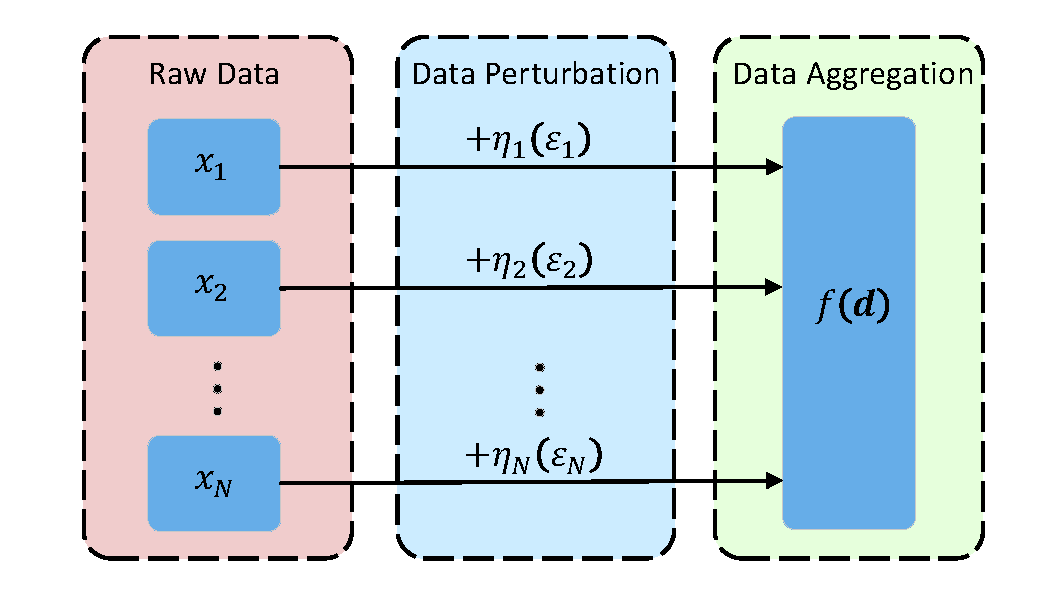
\includegraphics[scale=0.5]{./pic/pert.pdf}
\caption{An illustration of the local data perturbation and data aggregation processes.}\label{pert}
\end{figure}

We define $n_l^t=\sum_{i=1}^N\mathds{1}\{\epsilon^t_i=\epsilon_{(l)}\},~l\in\{1,\cdots,L\}$ as the number of users whose privacy-preserving levels equal to $\epsilon_{(l)}$ at stage $t$, and define the vector $\mathbf{n}^t=(n^t_1,\cdots,n^t_L)$ as the overall privacy-preserving level profile of the mobile crowds. We further denote $\mathbf{p}^t=(p^t_1,\cdots,p^t_L)\in P$ as a pricing profile specified by the platform, where each element $p^t_l\geq0$ indicates the payment to the user with $DPL=\epsilon_{(l)}$. We let $R(\mathbf{n}^t)$ denote the reward perceived by the platform at stage $t$, which is a function of the overall privacy-preserving level profile $\mathbf{n}^t$. The utility of the platform at stage $t$ is defined as the difference between the reward and the total payment, i.e., $u^t_0=R(\mathbf{n}^t)-\mathbf{p}^t\cdot\mathbf{n}^t$. Finally, we define the individual payoff of each user $i\in\ca{N}$ as $u^t_i=p_l^t-\epsilon_{(l)}c^t_i$, where $c^t_i$ is the unit privacy cost of user $i$ at stage $t$. 

\subsection{Q-learning based Dynamic Pricing}
At each stage of our MCS, user $i$ would drop out from participation if the monetary payment could not compensate their privacy loss, i.e., $\max_{\epsilon\in E} u^t_i(\epsilon,\mathbf{p}^t)<0$. Otherwise, user $i$ participates and chooses the $DPL$ that maximizes her payoff, that is, $\epsilon_i^*=\arg\max_{\epsilon\in E}u_i^t(\epsilon,\mathbf{p}^t)$. Next, user $i$ reports to the platform about her $DPL$ as well as the noisy sensing data, which is perturbed in a differentially-private manner parameterized by her $DPL$. Worth noting is that although the platform knows the $DPL$ of each user, she is incapable to restore the original data of each user with high confidence, which fulfills the effective protection of users' data privacy. 
%with probability $1-\delta_i$, and sets her $DPL$ randomly to each of the rest $L-1$ levels with probability $\frac{\delta_i}{L-1}$. The reason of introducing randomness to the decision making is because in reality it might be difficult for the user to perfectly evaluate her payoff

Observing that mobile users' unit privacy costs $\{c^t_i\}_{i\in\ca{N}}$ are time-varying and unknown to the platform and other mobile users, we resort to a learning based approach which is designed to enable the platform to learn out the optimal pricing policy via trial and error. 
\begin{figure}[h]
%\hspace{-0.35cm}
\centering
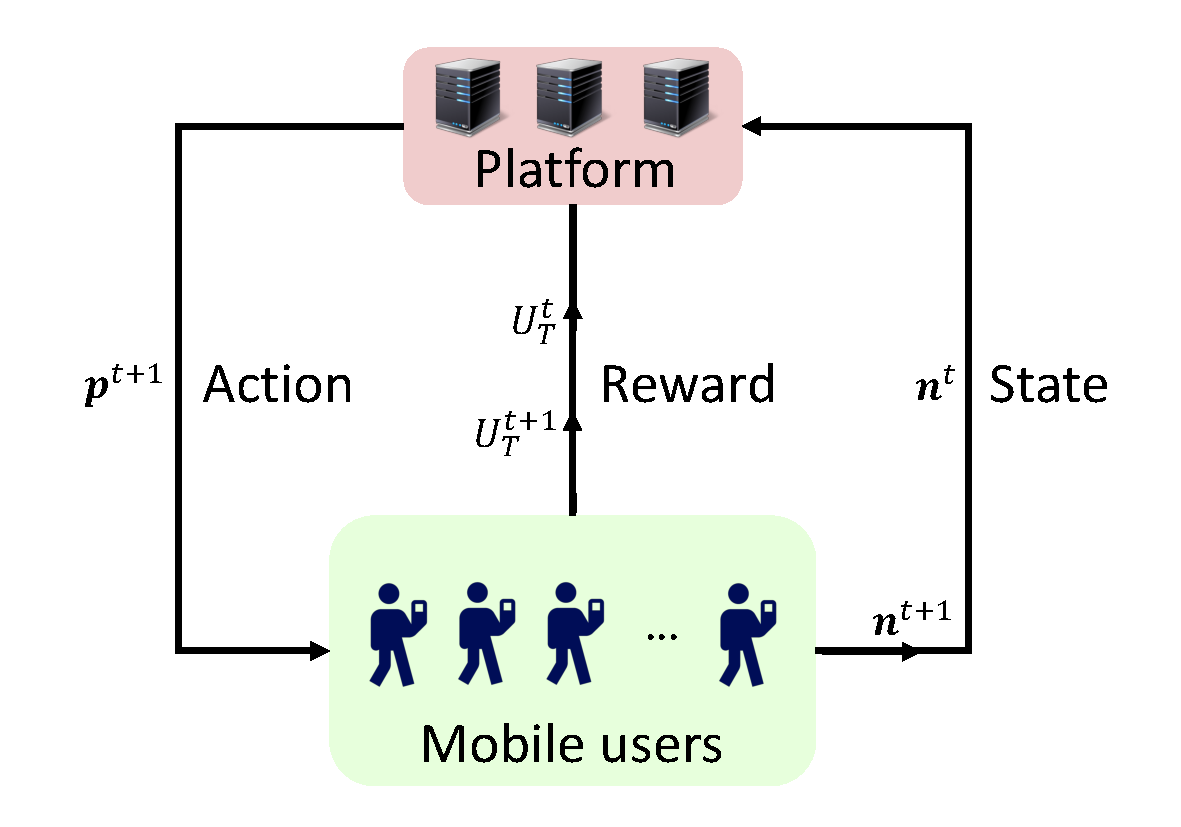
\includegraphics[scale=0.44]{./pic/rl2.pdf}
\caption{An illustration of the principle of the Q-learning based dynamic pricing mechanism.}\label{RL}
\end{figure}
Recently, Xiao \textsl{et al.} casted the interaction between MCS platform and selfish mobile users as a dynamic game and modeled the pricing process of the platform to a Markov Decision Process \cite{Xiao}. Inspired by \cite{Xiao}, we model the MCS platform's pricing process as a Markov Decision Process (MDP). Different from\cite{Xiao}, we do not address the pricing problem from the game-theoretic perspective. In our model, the state space of MDP corresponds to the overall privacy-preserving-level profile, i.e., $\{\mathbf{n}\}\subseteq\mathds{R}^{L}$. We device a Q-learning based algorithm for solving the MDP\cite{Sutton98a}. Specifically, we let $Q(\mathbf{n}^t,\mathbf{p}^t)$ denote the Q-function of state and pricing policy at stage $t$. The platform updates the Q-function according to the following procedure:
\begin{equation}\label{update}
\begin{cases}
Q(\mathbf{n}^t,\mathbf{p}^t)=(1-\alpha)Q(\mathbf{n}^t,\mathbf{p}^t)+\alpha(u^t_0(\mathbf{n}^t,\mathbf{p}^t)+\eta V(\mathbf{n}^{t+1})),\\
V(\mathbf{n}^t)=\underset{\mathbf{p}}{\max}Q(\mathbf{n}^t,\mathbf{p}).
\end{cases}
\end{equation}
where $\alpha\in(0,1]$ is the learning rate, $\eta\in[0,1]$ is the discount factor indicating the myopic nature of the server, $V(\cdot)$ is the highest value of the state. The principle of the learning process is illustrated in Fig. \ref{RL}. The platform is assumed to apply the $\sigma$-greedy policy to determine her pricing strategy $\mathbf{p}$ at each stage. Specifically, the optimal price $\mathbf{p^*}=\arg\max_{\mathbf{p}}Q(\mathbf{n}^{t+1},\mathbf{p})$ will be chosen with probability $1-\sigma$, and the other payment policies are uniformly randomly chosen with relatively smaller probability. The Q-learning based dynamic pricing mechanism for the platform is summarized in Algorithm \ref{alg:Q}.

\begin{algorithm}
\caption{Q-learning based dynamic pricing in MCS}
\label{alg:Q}
\begin{algorithmic}[1]
\STATE \textbf{initialization:}
\STATE Set $\alpha\in(0,1]$, $\eta\in[0,1]$, $Q(\mathbf{n},\mathbf{p})=0$, $V(\mathbf{n})=0$, $\forall\mathbf{n}, \mathbf{p}$.
%\State \textbf{end initialization}
\STATE Observe the initial system state $\mathbf{n}^0$;
\FOR {$t=1,2,3,...$}
\STATE Choose the pricing strategy $\mathbf{p}^t=\arg\max_{\mathbf{p}}Q(\mathbf{n}^{t+1},\mathbf{p})$ with probability $1-\sigma$; otherwise, randomly select a pricing policy $\mathbf{p}^t\in P$ with probability $\frac{\sigma}{|P-1|}$.
\STATE Observe the system state by calculating $\mathbf{n}^t=(n^t_1,\cdots, n^t_L)$.
\STATE Calculate the immediate utility $u^t_0$;
\STATE Update $Q(\mathbf{n}^t, \mathbf{p}^t)$ according to (\ref{update});
\STATE Update $V(\mathbf{n}^t)$ according to (\ref{update});
%\State Count down until the timer expires.
%\State $t\leftarrow t+1$
%\State \emph{`Faster' learning process:}
%\State Enquiry social neighbors' individual utility and compute instantaneous social group utility $S_{n}^t(a^t_n)$.
%\State Update estimation of expected payoff $\hat{R}_{n}^t(a^t_n)$ according to (\ref{estimation}).
%\State \emph{`Slower' learning process:}
%\If{the user $n$'s timer expires}
%\State Calculate the smooth best response $b^t_n(a_{n};\vv^t_{n},\beta)$ according to (\ref{sbr}).
%\State Update the mixed-strategy vector $q^t_n(a_n)$ according to (\ref{strategy}) and choose a channel $a^{t+1}_n$ according to $q^t_n(a_n)$.
%\EndIf
\ENDFOR
\end{algorithmic}
\end{algorithm}


\subsection{Case Studies}
In this section, we demonstrate the performance of our Q-learning based dynamic pricing mechanism through simulations. We set the default number of agents in the system as $N=200$, and the four possible $DPL$s  as $\epsilon_{(1)}=0.1$ (very high level), $\epsilon_{(2)}=0.2$ (high level), $\epsilon_{(3)}=0.3$ (medium level), and $\epsilon_{(4)}=0.4$ (low level). 
%Specifically, when user $i$ is in a state with highly-sensitive personal data, the monetary compensation from the platform might not be able to compensate her privacy cost (i.e., $\max_{\epsilon\in E} u^t_i(\epsilon,\mathbf{p}^t)<0$). In this case, user $i$ would set her $DPL$ to $\epsilon_{(0)}$ if $\max_{\epsilon\in E} u^t_i(\epsilon,\mathbf{p}^t)<0$, in which case the user's privacy . Otherwise, user $i$ sets her $DPL$ to $\epsilon^*=\arg\max_{\epsilon\in E}u_i^t(\epsilon,\mathbf{p}^t)$ with probability $1-\delta_i$, and sets her $DPL$ randomly to each of the rest three levels with probability $\delta_i/3$. The reason of introducing randomness to the 
%among other options eveandparticipates and specifies her $DPL$ according to a $\delta$-greedy policy \cite{Xiao} as follows:
%\begin{equation}
%\pi^t(\epsilon_i^t)=
%\begin{cases}
%1-\delta_i,~\epsilon^t_i=\epsilon^*=\arg\max_{\epsilon\in E}u_i^t(\epsilon,\mathbf{p}^t),\\
%\delta_i/3,~\epsilon^t_i=\epsilon_{(l)},~\forall\epsilon_{(l)}\in E/\{\epsilon^*,\epsilon_{(0)}\}.
%\end{cases}
%\end{equation}

Following equation (2.2) in \cite{DejunJ}, we define the reward function of the platform as $R(\mathbf{n}^t)=M\log(\mathbf{a}\cdot\mathbf{n}^t+1)$. The \emph{log} function characterizes the platform's diminishing return on users' participations. And the scaling factor $M$ is a system parameter customized by the platform. The weight vector $\mathbf{a}=(a_1,a_2,a_3,a_4)$ quantifies the contribution of sensing data from users with different privacy-preserving levels, and is set as $\mathbf{a}=(2, 1.5, 1, 0.5)$ in our case study. For ease of exposition, we generate the unit privacy cost of each user at a single stage according to \emph{iid} normal distribution, i.e., $c_i\sim\mathcal{N}(\mu,0.1)$. Empirically, we set the parameters for our learning algorithm as $\alpha=0.2$, $\eta=0.8$, and $\sigma=0.2$. 

We run the experiments for different levels of users' mean unit privacy costs (i.e., $\mu=1.0, 1.5, 2.0$). Fig. \ref{conv} shows the changing trend of platform utility as the number of iterations increases under different values of user's mean unit privacy cost $\mu$. It can be seen that our algorithm converges quickly after 300 iterations. The result also indicates that the achievable utility of platform is larger for smaller unit privacy cost. In Fig. \ref{cmax}, we illustrate the effect of total number of users on the platform's utility. Specifically, as the number of users increases from 100 to 300, the achievable utility increases monotonically for all three cases of different mean unit privacy cost. In addition, it can be observed that the marginal increase of utility reduces as the total number of users increases. This is due to the concave property of the reward function we used in our case study, which also agrees with the fact that after enough amount of sensing data being collected, the value brought by the newly collected data will shrink.



\begin{figure}[t]
%\hspace{-0.35cm}
\centering
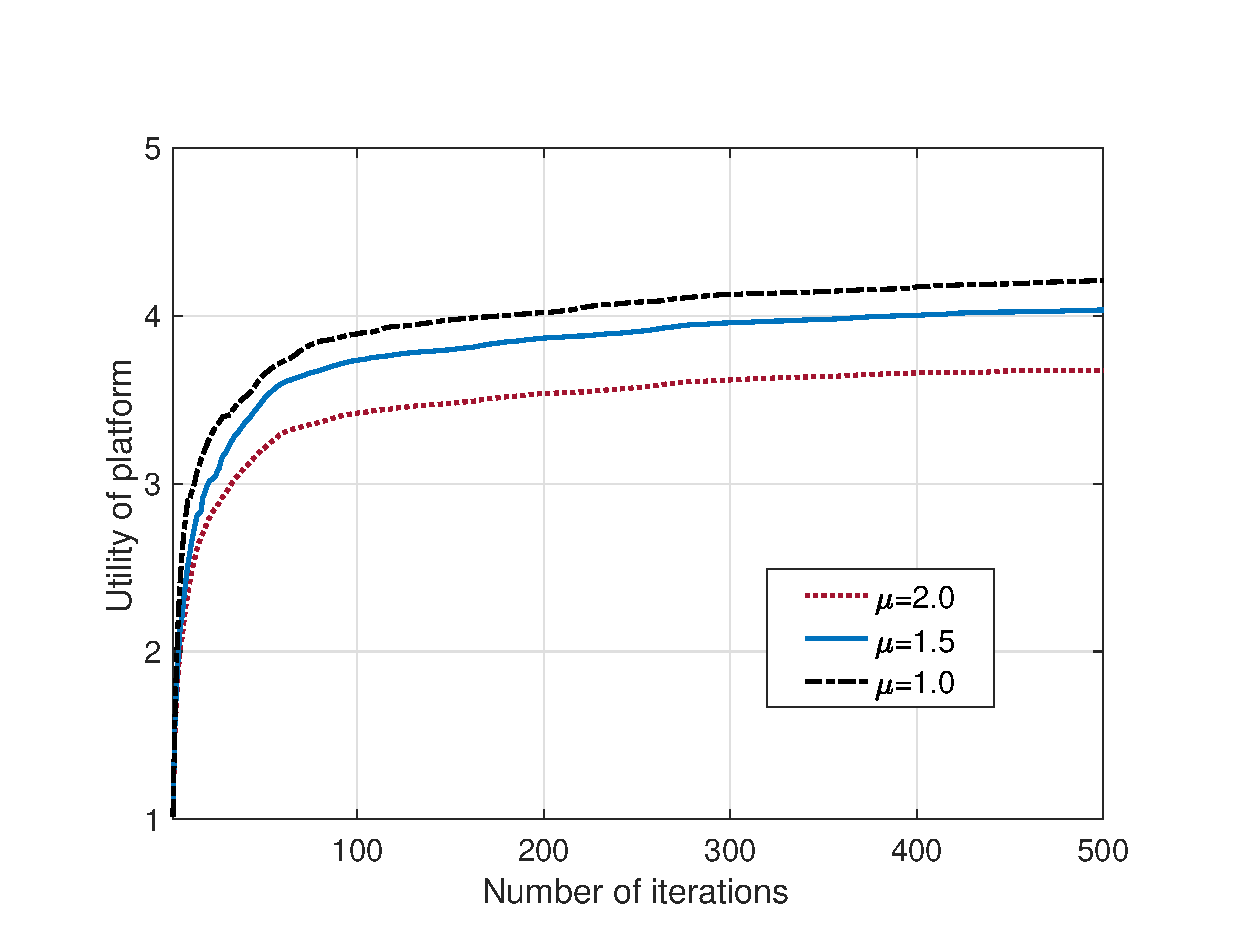
\includegraphics[scale=0.44]{./pic/conv4.eps}
\caption{Illustration of the convergence performance of the learning algorithm.}\label{conv}
\end{figure}
\begin{figure}[t]
%\hspace{-0.35cm}
\centering
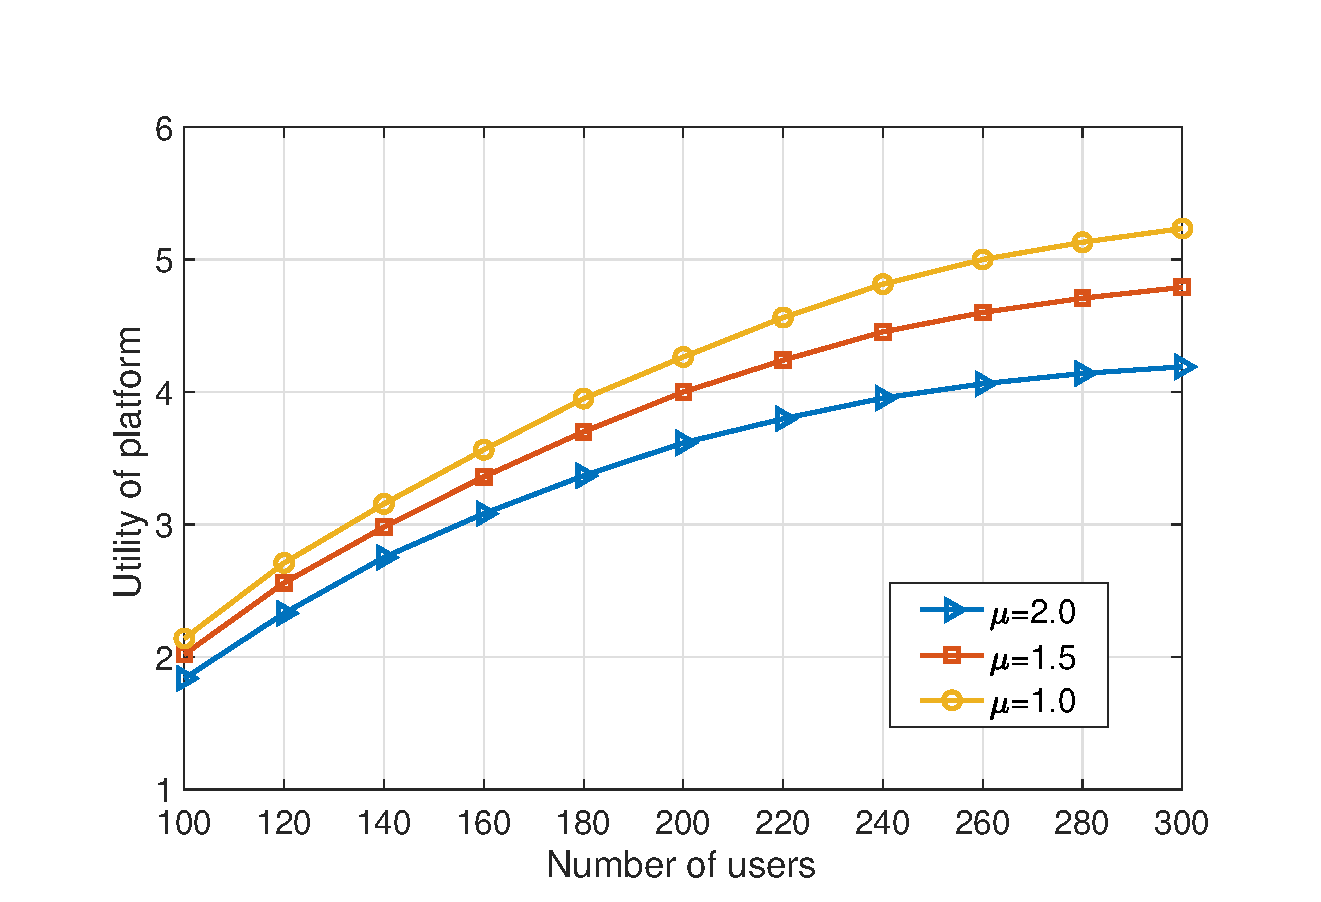
\includegraphics[scale=0.44]{./pic/u_num4.eps}
\caption{Illustration of the impact of amount of users on the platform utility.}\label{cmax}
\end{figure}


\section{Conclusion}\label{sec:s5}
In this article, we give an overview of several state-of-art privacy-preserving approaches for mobile crowdsensing that stimulate the participation of mobile users with privacy concerns of releasing their sensitive data. To address the challenge that participated users' privacy-preserving requirements may be time-varying, we proposed a Q-learning based pricing mechanism through which the MCS platform can dynamically adapt its pricing policy to optimize its utility. A case study is further provided to evaluate the performance of our proposed approach.



\chapter{双重网络外部性下移动数据服务提供商收益最大化研究}

\textbf{本章摘要:} 
移动社交网络极大地增强了人们的在线社交互动,产生了海量的移动数据流量,为无线服务提供商带来了可观的收入。然而,潜在的收入增长正面临着通信基础设施网络容量的限制,以及服务提供商之间竞争的影响。本章研究了竞争性数据服务市场中多个服务提供商的定价策略,其中移动用户的数据消费行为受到两方面因素的影响:社交效应(正网络外部性)和拥塞效应(负网络外部性)。为了分析移动用户和服务提供商之间的策略互动,我们设计了一个两阶段的斯塔克伯格博弈,分别由第一阶段的提供商博弈和第二阶段的用户博弈组成。针对用户博弈,本章刻画了均衡解的特征并建立了它的唯一存在性。对于提供商博弈,本章的分析表明,在提供商行为理性的场景以及提供商行为有限理性的场景下,混合策略均衡解的存在性都是有所保证的。进一步,本章提出了一种分布式学习算法,用于寻找混合策略均衡解决方案。本章第6节的的数值仿真结果对于社交效应和拥塞效应如何影响系统性能提出了见解,并验证了提供商有限理性行为为其收益带来的损失。

%Mobile social networks have greatly strengthened people's online social interactions, generating massive volume of mobile data traffic, and bringing remarkable revenues to the wireless service providers. Meanwhile, the potential revenue growth is restrained by the network capacity of physical communication infrastructure, and also challenged by the competition among service providers themselves. In this paper, we study the pricing strategies of multiple service providers in a competitive data service market, where mobile users' data consumption behaviors are influenced by two effects: the positive network effect and the congestion effect. To analyze the strategic interactions between mobile users and service providers, we device a two-stage Stackelberg game consisting a pricing game in Stage I and a usage game in Stage II, respectively. In particular, for the usage game, we characterize the equilibrium solution and establish its uniqueness. For the pricing game, our analysis indicates that a mixed-strategy equilibrium solution is guaranteed for the scenario with rational providers as well as the scenario with providers of bounded rationality. We further develop a distributed learning algorithm for finding a mixed-strategy equilibrium solution in the second scenario. Our numerical results provide insights into how positive network effect and congestion effect would impact the system performance, and demonstrate that the bounded rational behavior incurs degradation to service providers' revenues.

\textbf{关键词:}移动社交网络;网络定价;网络外部性;博弈论;展望理论
%\keywords{多目标跟踪;实时性;整数规划}

\section{引言}

在过去的十年中,人们对于移动智能设备的使用量经历了巨大的增长。对于不同背景和年龄的人群,移动智能设备如今已然成为他们日常生活中不可或缺的一部分。近年来,智能设备的普及也同时给在线社交网络(例如Facebook \cite{FB},Twitter \cite{Twitter})带来了巨大成功,极大地促进了人们的在线社交互动。统计数据显示,由于智能设备和在线社交网络的激增,全球移动社交用户数量早在2017年1月就已超过25亿,占社交媒体用户总数的91%\cite{Wearesocial}。
%The use of smart devices has experienced immense growth in the past decade, becoming an indispensable part of the daily life for most people around world, regardless of their backgrounds and age. In line with the pervasive penetration of smart devices, recent years have also witnessed the spectacular success of online social networks (e.g., Facebook\cite{FB}, Twitter\cite{Twitter}), which have greatly strengthened people's online social interactions.  Attributed to the proliferation of both smart devices and online social networks, the mobile social users has increased by 30\% year-over-year to surpass 2.5 billion globally in January 2017, accounting for 91\% of the total social media users \cite{Wearesocial}.

移动社交用户的激增不仅为社交网络平台带来了丰厚的利润,而且还为无线服务提供商带来了可观的收入。直观上,如今市场上众多经过精心设计的移动社交应用程序,使得人们可以随时随地与他们现有的朋友或未曾相似的用户进行在线互动(通过互发信息,多媒体共享和在线游戏等方式)。在这种{\kaishu 正网络外部性}作用\cite{David10}下,用户间社交关系的增强与扩展会反过来激发更多数据流量消费。例如,市场调研结果表明,如果某个手机游戏在一个用户的社交好友圈中非常受欢迎,那么该用户通常也会更喜欢玩该游戏。心理学上对这种潜在影响的分析为:个体通常希望自己可以被视为同伴中的一部分。这种正网络外部性可以在整个移动社交网络中广泛传播,从而导致数据使用量整体激增,为无线提供商带来可观的潜在收入。
%The explosion of mobile social users not only brings remarkable profit to the social network platforms, but also delivers great revenues to the wireless service providers. Intuitively, mobile social applications are well-designed nowadays to encourage peopzule's online interaction with either their known friends or other unacquainted users anytime and anywhere (e.g., via messaging, media sharing, and online gaming, etc.). The strengthened and expanded social relationship will in turn give rise to greater data consumption owing to {\em positive network effect}\footnote{The network effect is a concept in economic and business describing that the value of a good or service to one user is influenced by others' valuation on that good or service. A positive network effect normally refers to the phenomenon whereby a product or service becomes more valuable as more people accept it, encouraging ever-increasing numbers of users.\\}\cite{David10}. For instance, a user usually becomes more involved into playing a mobile game if that game has gained much popularity among her social friends. A psychological explanation of this effect is that users always want to be perceived as part of their peers.
%As another example, a user online video-streaming, her social friends are playing the same mobile gameher friendsor watching an online streaming video if her social friends areor the public, even if she is not quite interested into it at the beginning. 
%Such kind of positive network effect could be conveyed extensively throughout the mobile social network, resulting a fire-up of data consumption that has potential to generate significant revenues for the wireless providers. 
然而与此同时,无线通信网络的有限容量已逐渐成为正网络外部性下流量增长的主要制约。以在线手机游戏平台为例,由于无线通信带宽有限,在每天高峰时间段,活跃用户数量的增加以及所产生的累积数据流量时常导致数据传输的拥塞与服务的延迟。这种{\kaishu 负网络外部性}效应下用户体验上的影响将降低那些对延迟较为敏感的用户的活跃度,给服务提供商带来收入上的损失。
%However, with increasingly many on-the-shelf mobile applications being data-hungry, the potential growth of providers' revenues from network effect is constrained by the capacity of wireless communication network. Take the online mobile game platform as an example, the increasing number of active users at the peak time and the generated accumulated data traffic will result in serious congestion (hence service delays) due to limited bandwidth. And the resulted bad user experience would discourage users' data usage in such kind of delay-sensitive applications, which brings revenue loss to service providers.

使用合理的定价机制是一种重要的网络流量调控手段。传统通信网络中的定价问题已经在文献\cite{Walrand08,Huang10,Xinbin,CaoTVT,Xiaoming}中得到了较好的解决。对于移动无线通信网络中的定价问题,一些研究工作也已经将用户数据使用行为所受到的正网络外部性影响考虑进来\cite{Hartline08,Candogan12,SwapnaES12}。
近期,Gong等\cite{GongDCZ17}对单一服务提供商的无线数据服务市场中移动用户在网络效应和拥塞效应下数据消费行为进行了研究。然而在一些现实场景中,移动用户已经不再局限于单个服务提供商,而是可以选择从多个无线服务提供商购买服务\footnote{例如,在美国,移动用户可以通过订阅例如Google的Project Fi \cite{GoogleFi}这样的虚拟网络运营商来使用T-mobile和Sprint的数据服务。}。另一方面,实际中的一些迹象表明个体决策通常会偏离期望效用理论(Expected Utility Theory)框架\cite{Von}所预期的理性决策。在行为经济学领域进行的一些现有研究工作\cite{camerer2011behavioral}指出,个体的非理性行为时常归因于以下事实:当面对竞争和不确定性时,不同的个体会对他们的风险和收益进行不同且主观的评估。基于以上的观察与发现,本章考虑了多个服务提供商策略性争夺无线服务市场份额的问题场景,研究了在双重网络外部性效应下服务提供商以最大化其业务收益为目标的定价机制设计问题,并在建模中对于提供商的一些非完全理性行为进行了充分的考量。

%以上这些发现,使得对无线服务商寡头市场中定价决策的研究变得尤为有意义。
%Recently, the authors in\cite{GongDCZ17} have investigated the mobile users' data consumption behavior under both the network effect and the congestion effect in a single wireless service provider market. Meanwhile, instead of being restricted to a single service provider, mobile users nowadays have had the option to purchase services from multiple wireless service providers\footnote{For example, mobile users can subscribe to the service of both T-mobile and Sprint via virtual network operator such as Google's Project Fi \cite{GoogleFi}.}. Motivated by this observation, this study considers a scenario where multiple service providers need to compete strategically for the shares of the wireless service market to maximize their business revenues. Another observation inspiring this study is that individuals' decision making in reality usually deviate from the rational ones expected according to the well-established Expected Utility Theory framework \cite{Von}. Some existing research works done within the field of behavior economics \cite{camerer2011behavioral} have indicated that the irrationality is attributed to the fact that different individuals would have different and subjective evaluations on their risks and revenues when facing with competitions and uncertainties in practice.
%In order to optimize their utilities, the mobile users thereby need to strategically determine their data consumption from each of the service providers, with consideration of the social influence and congestion effect. On the other side, multiple service providers have to compete against each other for mobile users by adjusting their service prices in order to maximize their revenues in the market. Further, 
%With all these insights, it is of great interest to study the pricing-usage decision interaction in an oligopoly market of multiple wireless service providers.

简而言之,本章研究了一个具有多个服务提供商的竞争型无线数据服务市场,其中移动用户在确定其数据使用量时同时考虑两方面因素的影响,即对应于正网络外部性的社交效应以及对应于负网络外部性的拥塞效应。本文使用斯塔克伯格(Stackelberg)博弈\cite{osborne}的模型将提供商定价问题与用户数据使用问题结合起来进行建模。当博弈中服务提供商和个人用户的策略行为达到均衡状态时,任何独立的个体无法通过改变其策略获得更好的自身效用。对于刻画用户博弈均衡时的一个挑战在于每个用户的策略空间为多维空间(每个用户可以同时选用多个服务提供商的数据服务)。为了应对这一挑战,本文将连接任一用户和任一提供商的链接视为一个“虚拟用户”,并相应地对于每个“虚拟用户”的数据使用量进行考量。具体来说,在博弈的第一阶段,提供商会审慎地对其数据服务的单价进行设置以最大程度提高其潜在收益。在博弈的第二阶段中,给定每个提供商的单位数据服务价格,每个“虚拟用户”会策略性地确定其数据使用量,以优化其自身所获得的效用。在满足一定条件时,“虚拟用户”之间博弈均衡解的存在性以及唯一性可以被证明。在此基础上,可以进一步证明提供商定价博弈中$\epsilon$-混合策略价格均衡的存在性。
%In a nut shell, this paper studies a wireless service market with multiple competitive service providers, and a group of data consuming mobile users that strategically determine their data usage subject to the two different effects, namely positive network effect and congestion effect. To this end, we formulate the pricing-usage problem as a \emph{Stackelberg game}\cite{osborne}, in which service providers and individual users determine their strategies aiming to get to an equilibrium state, where no one could be better off by unilaterally deviate from the equilibrium point. One key challenge in characterizing the game lies in the high dimensionality of each user's strategy space. To tackle this challenge, we treat each link connecting one user and one provider as a ``virtual user'', and quantify the data usage of each ``virtual user'' accordingly. Specifically, in Stage I of the game, providers deliberately set the unit price of their data service in order to maximize her potential revenue. In Stage II, each ``virtual user'' determines her data usage strategically to optimize the corresponding payoff, given the service price of each provider. Under some technical conditions, we show both the existence and uniqueness of the equilibrium solution among ``virtual users'', based on which, we further show the existence of an $\epsilon$-mixed-strategy pricing equilibrium for the providers.

为了描述有限理性提供者的定价决策行为,本章第5节应用{\kaishu 展望理论}\cite{Kahneman}对第一阶段提供商之间的定价博弈作了进一步分析研究。作为诺贝尔经济学奖获奖理论,展望理论被用以模拟和解释存在风险和不确定性下的个人决策\cite{Tianming,Yu},并已被应用于一些实际问题场景中。例如,Li等\cite{Tianming}研究了一种无线环境下的随机接入博弈,其中用户考虑了展望理论中的{\kaishu 概率失真效应}作用,策略性地确定其在冲突信道上的传输概率。
%Yu等\cite{Yu}研究了一种数据市场模型,模型中用户需要选择成为数据卖方还是数据买方,并确定交易的数据量。他们考虑了展望理论中的{\kaishu 概率失真效应}和{\kaishu 效用框架效应}对用户决策行为的影响,并将该问题表述为非凸优化问题。
本章同时考虑了展望理论所涉及的两个主要现象:{\kaishu 概率失真效应}和{\kaishu 效用框架效应}。本章的分析表明,在这两种效应影响下​​,给定一定条件,$\epsilon$-混合策略定价均衡仍然存在。由于这种情况下服务提供商的收益函数不再被假设为已知信息,本文诉诸于分布式学习算法,使得服务提供商通过观察到的部分信息可以学习得到$\epsilon$-混合策略的定价均衡。数值结果表明,提供商的有限理性行为最终会导致其期望收入的下降。
%In order to characterize the pricing behaviors of bounded rational providers, we further study the pricing game in Stage II by appealing to \emph{Prospect Theory}\cite{Kahneman}. This Nobel-prize-winning theory has been utilized in several real-life applications to model and explain individuals' decisions under risks and uncertainty \cite{Tianming, Yu}. In this study, we particularly consider two main aspects of Prospect Theory: the \emph{probability distortion effect} and the \emph{utility framing effect}. We show that the existence of an $\epsilon$-mixed-strategy pricing equilibrium still holds under the two effects given a mild condition. Since service providers' payoffs are no longer public information, we resort to a distributed learning algorithm, by which service providers with partial observation can learn to play out an $\epsilon$-mixed-strategy pricing equilibrium. Through numerical results, we show that the expected revenue of provider suffers from a degradation as a result of providers' bounded rational behaviors.

本章的剩余部分组织如下。第\ref{sec:tvtmodel}节描述了无线服务提供商和移动用户之间的两阶段斯塔克伯格博弈的基本建模。第\ref{sec:stageII}节研究了针对用户之间流量使用的用户博弈,并描述了博弈的联边需求均衡解。第\ref{sec:stageI}节对提供商之间的定价博弈进行讨论和分析。最后,第\ref{sec:stageI2}节从展望理论的角度重新审视了服务提供商之间的定价博弈问题。相关的数值仿真结果在第\ref{sec:sim}节中给出,第\ref{sec:tvtcon}节对本章进行了总结。
%The remainder of the paper is organized as follows. We first discuss the related work in Section \ref{sec:related}. In Section \ref{sec:model}, we describe the basic formulation of the two-stage Stackelberg game between wireless service providers and mobile users. In Section \ref{sec:stageII}, we study the usage game among mobile users and characterize the link demand equilibrium of the game. Then we study the pricing game among providers in Section \ref{sec:stageI}, followed by the Section \ref{sec:stageI2} which revisits the pricing game by appealing to Prospect Theory. Numerical results are given in Section \ref{sec:sim}, and Section \ref{sec:con} concludes the paper.

%\section{研究现状}\label{sec:tvtrelated}
%
%在通信网络中,当流量负载增加到超出基础架构的物理性质确定的容量时,就会发生拥塞。拥塞效应在一些数据速率较低的通信场景(例如\cite{Jiming}和\cite{Deng})中的影响可能并不突出。然而它的影响在许多数据通信速率较高的系统中变得尤为显著,目前已有相关文献对其做了进行了深入的研究(参见\cite{Asuman07,Fang09,Tran12}及其中的参考文献)。
%%In communication networks, congestion occurs as traffic load increases beyond the capacity determined by the physical nature of the infrastructure. The impact of congestion effect might not be prominence in some low-data-rate communication schemes (e.g., \cite{Jiming} and \cite{Deng}). While it is much more significant in many high-data-rate communication systems and has been studied extensively in related literatures (see, e.g. \cite{Asuman07,Fang09,Tran12} and the references therein). 
%
%近年来,移动网络的社交影响引起了服务提供商以及平台开发人员的广泛关注。如今,越来越多的移动用户通过在线社交网络(例如Facebook \cite{FB},Twitter\cite{Twitter})进行联络,用户的影响力和信息传播速度比以往任何时候都快\cite{Niyato}。在\cite{David10}中,作者将用户之间的社交效应建模为一种正面的网络效应。在\cite{Baochun}中,作者采用了类似的想法来刻画众包系统中不断增长的社交用户数量所带来的内在收益的增长,及其对于平台所应提供的部分外在奖励的节省。在\cite{social}中,为了减少峰值蜂窝负载,作者提出了一系列算法根据用户在社交网络中的位置选择出特定用户,并将内容主动地推送给这些用户。
%%In recent years, the social aspect of mobile networking has attracted much attention of service providers and also platform developers. As more and more mobile users are nowadays connected by online social networks (e.g., Facebook \cite{FB}, Twitter \cite{Twitter}), both the influences and information of users can propagate within the crowds faster than ever \cite{Niyato}. In \cite{David10}, the social effect among users has been modeled as a kind of positive network effect. In \cite{Baochun}, similar idea was adopted to characterize the effect that growing population of socially connected users in crowdsourcing system results in more intrinsic rewards, which helps save a part of extrinsic rewards that are supposed to be provided by the platform. In \cite{social}, in order to reduce the peak cellular load, the authors proposed a family of algorithms that proactively push content to particular users that are selected based on their positions in the social network. 
%
%在另外一些研究工作中,个体间的社交影响已经被用在解决许多网络设计和优化问题中。Chen等\cite{Chen13}利用社交信任和互惠互利因素,通过将问题转化为联盟博弈来改进D2D合作通信。XX等人则利用用户之间的社交距离进行用户关联,以增强具有底层D2D通信的小型蜂窝网络的系统性能\cite{Ashraf}。Yang等\cite{Guang}提出了一种移动群智感知系统设计,利用移动用户之间的社交联系来激励他们的参与和合作,以获取更高的回报。Chen等\cite{Chen14}提出了一个社交团体效用最大化(SGUM)框架,其中每个用户关注的是由自己的个人效用与社交朋友的效用所组成的“团体效用”。
%%Along another line of literatures, social influences among individuals have been utilized in solving many network design and optimization problems. In \cite{Chen13}, Chen \emph{et al.} have leveraged social trust and social reciprocity to enhance cooperative D2D communication by casting the problem to a coalitional game. In\cite{Ashraf}, the social distances between user equipments were exploited for the user association to enhance the system performance of a small cell network with underlaid D2D communication. 
%%In \cite{Huang17}, Cheung \emph{et al.} proposed a socially-aware reward mechanism for mobile crowdsensing system, where the platform exploits users' social relationship for profit maximization. 
%%In \cite{Guang}, Yang \emph{et al.} proposed a mobile crowd sensing system design that leverages social ties among mobile users to incentivize their participation and global cooperation for higher payoffs. In \cite{Chen14}, the authors developed a social group utility maximization (SGUM) framework, in which each user cares about the ``group utility'' consisting of her own utility as well as her social friends' utilities.  
%
%通信网络中的定价问题已经在文献\cite{Walrand08,Huang10,Xinbin,CaoTVT,Xiaoming}中得到了较好的解决。在一些重点关注单个服务提供商定价策略的研究工作中,移动用户的数据使用行为所受到正面网络影响已经被考虑进来,如\cite{Hartline08,Candogan12,SwapnaES12}。而据我们所知,目前还很少有在研究网络服务定价问题中同时考虑到网络效应和拥塞效应的影响。最近,Gong等\cite{GongDCZ17}首先研究了垄断市场中单个服务提供商的定价策略,在该市场中,移动用户的数据使用行为会同时受到这两种影响。相比于上述工作中所考虑的垄断市场,我们的前期工作\cite{MYCISS16}研究了寡头市场环境下的定价问题,即存在多个服务提供商之间争夺移动用户的数据市场的竞争。
%%The pricing problem in communication networks has been addressed extensively in the literature \cite{Walrand08,Huang10,Xinbin,CaoTVT,Xiaoming}. There has been a line of works focusing on investigating the pricing strategies of a single service provider, with the mobile users' data usage behavior subject to positive network effect (see, e.g., \cite{Hartline08,Candogan12,SwapnaES12}). 
%%Hartline \emph{et al.} propose a basic ``Influence and Exploit Marketing'' strategy in \cite{Hartline08}, which takes into consideration of sequential purchases, where myopic consumers make their consumption decisions based on their neighboring consumers who have already bought the product. Candogan \emph{et al.} in \cite{Candogan12} consider a simultaneous consumption decision making model for rational agents embedded in a social network. They formulate the interactions between the monopolist and agents as a Stackelberg game with linear-quadratic utility function for the agents. 
%%To the best of our knowledge, very little works on network pricing have considered the impact of both network effect and congestion effect. 
%%\cite{Johari10} has studied users' behaviors, when they experience both network effect and congestion effect. However, it assumes that the network effect is the same for all users, which does not capture the fact that users experience different levels of network effect based on their diverse social ties as considered in this paper. 
%%The authors in \cite{GongDCZ17} first studied the pricing strategy of a single service provider in a monopoly market where mobile users' data usage behaviors are subject to both the two effects. In contrast to \cite{GongDCZ17}, our preliminary work \cite{MYCISS16} investigated the pricing problem in an oligopoly market setting, where multiple service providers compete against each other for mobile users' data consumption.
%
%近些年,人们在解决一些实际的无线网络中的决策问题时,采用了展望理论(Prospect Theory)\cite{Kahneman}对决策过程进行建模。 例如,Li等\cite{Tianming}研究了一种无线环境下的随机接入博弈,其中用户考虑了展望理论中的概率失真效应作用,策略性地确定其在冲突信道上的传输概率。Yu等\cite{Yu}研究了一种数据市场模型,模型中用户需要选择成为数据卖方还是数据买方,并确定交易的数据量。他们考虑了展望理论中概率失真效应和效用框架效应对用户决策行为的影响,并将该问题表述为非凸优化问题。
%%Recently, Prospect Theory \cite{Kahneman} has been employed to model the decision making process within wireless networks in practice. In \cite{Tianming}, Li \emph{et al.} studied a wireless random access game, where users strategically determine their transmission probabilities over a collision channel under the probability distortion effect of Prospect Theory. Yu \emph{et al.} in \cite{Yu} studied a data market model, where users need to choose to be a data seller or a data buyer, and also determine the amount of data being traded. They formulated the problem as a non-convex optimization problem considering both the probability distortion effect and the utility framing effect on users' decision behaviors. 
%
%在本文中,我们考虑了可能存在的服务提供商行为有限理性的情况。在这种更为一般性的背景下,我们证明了用户博弈的混合策略定价均衡的存在,并给出了均衡唯一的条件。我们的数值结果表明,服务提供商的有限理性行为会导致总收入下降。
%%虽然部分工作已在\cite{MYCISS16}中进行了介绍,但本文中已添加了主要结果的完整证明,以帮助读者更好地理解。
%%In this paper, we extend our discussion in preliminary work \cite{MYCISS16} to a broader scope by considering the case where service providers can be of bounded rationality. And in this more general setting, we show the existence of a mixed-strategy pricing equilibrium of a usage game, and establish the condition under which the equilibrium is unique. Our numerical result indicates that service providers' bounded rationality can lead to degradation on the total revenues. While part of this work has been presented in \cite{MYCISS16}, complete proofs for the main results have been added in this paper to facilitate readers' better understanding.

\section{社交关系影响下移动数据的价格竞争}\label{sec:tvtmodel}

在本节中,我们首先提出了无线数据服务的寡头市场模型,在该模型中,互相之间具有社交关系的移动用户可以从一组服务提供商那里购买和使用数据服务。我们使用两阶段的\emph{斯塔克伯格博弈}对提供商和用户之间的交互进行建模。我们接下来对建模进行具体介绍。
%In this section, we first provide the oligopoly market model for the wireless data service, in which a crowd of socially connected mobile users can purchase and consume the data service from a group of service providers. We next describe the two-stage \emph{Stackelberg game} formulation that models the interactions between providers and users. 

%To tackle the challenge in characterizing the game in Stage II due to the multidimensional strategy space of each user, the data usage problem among users is cast as a game played by virtual players.

%\subsection{Socially-aware Mobile Data Usage and Wireless Providers' Pricing Strategies}
\subsection{系统模型}

我们考虑一组移动用户$\N\triangleq\{1,\cdots,N\}$从一组无线服务提供商$\K\triangleq\{1,2,\cdots,K \} $那里购买使用具有可替代性的无线数据服务\footnote{此处可替代性意味着使用来自不同服务提供商的等量数据对于用户来讲具有相同价值。}。每个用户可以从一个以上的服务提供商那里购买服务,其中用户$i$从服务提供商$k$消费的数据量(由$x^k_i$表示)。我们令$\mathbf{X}\in\mathbb{R}^{N\times K}$表示所有用户的使用情况,用$\mathbf{X}_{-i}$表示排除用户$i$后剩余用户的使用情况。
%Consider a set of mobile users $\N\triangleq\{1,\cdots,N\}$ consuming perfectly substitutable wireless services\footnote{Perfectly substitutable wireless services here means that the same amount of data usage from different service providers has the same valuation to a mobile user.} from a set of wireless service providers $\K\triangleq\{1,2,\cdots,K\}$. Each user can subscribe to more than one service providers with the data consumed by user $i$ from service provider $k$ denoted by $x^k_i$.
%Consider a market with a set of wireless service providers $\K\triangleq\{1,2,\cdots,K\}$, who provide perfectly substitutable wireless services\footnote{The same amount of data usage from different service providers has the same valuation to each mobile user.} to a set of mobile users $\N\triangleq\{1,\cdots,N\}$. Each user $i\in\N$ can subscribe to all $K$ service providers and the data usage consumed from service provider $k\in\K$ is denoted by $x_i^k$. 
%We let $\mathbf{X}\in\mathbb{R}^{N\times K}$ denotes the usage profile of all the users, and $\mathbf{X}_{-i}$ denotes the joint usage profile without user $i$.

我们假定移动用户之间存在社交关联,并使用社交联系量$g_ {ij}\in[0,1]$来量化用户$j$对用户$i$的社交影响。而社交影响所引发的{\kaishu 正网络外部性}使得移动用户随着其社交朋友数据使用量的增加获得更多的效用。
%The mobile users are assumed to be socially connected, with the social impact of user $j$ on user $i$ quantified by a positive social tie $g_{ij}\in[0,1]$. The social impact induces \emph{positive network effect}, under which mobile users are inclined to experience more utility gain as the usages of their social friends increase.
%which can be modeled by the product term $g_{ij}x_{i}^{k}x_j^k$ as in \cite{GongDCZ17} and \cite{Candogan12}.
%Due to the fact that social services encourage mobile users to demand more data usage (i.e., the positive network effect), we model this effect by using a social tie $g_{ij}\in[0,1]$ to quantify the social influence from user $j$ to user $i$. As in \cite{GongDCZ17} and \cite{Candogan12}, the product $g_{ij}x_{i}^{k}x_j^k$ can capture that a user derives more utility by increasing her usage in social services, and the marginal gain of social utility increases as her social friends increase their usage. 
另一方面,随着用户整体数据消耗的增加,拥塞效应(例如,服务延迟现象)作为一种{\kaishu 负网络外部性}效应将变得尤为显著。由此,本章在建模时所需要明确地将每个移动用户的个人效用分成四部分:固有效用,数据使用成本,社交效应和拥塞效应。具体来说,给定每个提供商收取的单位服务价格,用户$i$的单个效用可以写为
%As data consumption increases, the congestion effect (e.g., service delays) will become prominent, and need to be explicitly considered in our model. To this end, the individual utility of each mobile user includes four parts: the intrinsic utility, the data usage cost, the network effect, and the congestion effect. Specifically, given the unit service price charged by each provider, the individual utility of user $i$ can be written as
\begin{align}\label{eq:userU}
%\small
u_i&(\mathbf{x}_i,\mathbf{X}_{-i},\mathbf{p})=\underbrace{a_i\sum_{k\in\K}x^k_i-\frac{1}{2}b_i(\sum_{k\in\K}x^k_i)^2}_{\text{固有效用}}-\underbrace{\sum_{k\in\K}p_kx^k_i}_{\text{数据使用成本}}\nonumber\\
&+\underbrace{\sum_{k\in\K}x^k_i\sum_{j\in\N}g_{ij}\sum_{m\in\K}x^m_j}_{\text{社交效应(正网络外部性)}}-\underbrace{\frac{c}{2}\sum_{k\in\K,x_i^k>0}(\sum_{j\in\N}x^k_j)^2}_{\text{拥塞效应(负网络外部性)}},
\end{align}
其中$\mathbf{x}_i = (x_i^1,x_i^2,\cdots,x_i^K)$表示用户$i$的使用情况,而$\mathbf{p} = (p_1,\cdots, p_K)$表示所有服务提供商的定价策略,其中$p_k$表示来自提供商$k\in\K$的数据服务单价。同工作\cite{GongDCZ17}和工作\cite{Candogan12}相同,我们采用了二次函数形式的内在效用函数,其对类型广泛的一些凹函数来说是很好的二阶近似。具体来说,$a_i>0$和$b_i>0$是两个内在系数,用于表征使用数据服务对于用户$i$的固有效用。双重网络外部性中的社交效应被建模为来自用户$i$的总数据需求量的线性函数,因而其边际效用取决于其社交好友的总数据使用量乘以对应社会联系的加权总和(即$\sum_{j\in\N}g_{ij}\sum_{m\in\K}x^m_j$)。而对于双重网络外部性中的拥塞效应,本文建模中假设用户从单个服务提供商处所受到的拥塞影响与该服务提供商的总数据流量的平方成正比,其中参数$c>0$用以刻画物理通信介质的状况。用户受到的总拥塞影响是其受到各服务提供商拥塞影响的总和。
%where $\mathbf{x}_i=(x_i^1,x_i^2,\cdots,x_i^K)$ denotes the usage profile of user $i$, and $\mathbf{p}=(p_1,\cdots,p_K)$ denotes the joint pricing profile of all the service providers where $p_k$ denoting the unit price of data service from provider $k\in\K$. Following \cite{GongDCZ17} and \cite{Candogan12}, we apply a quadratic form intrinsic utility function, which serves as a good second-order approximation for a broad class of concave utility functions. Specifically, $a_i>0$ and $b_i>0$ are two intrinsic coefficients that characterize user $i$'s intrinsic valuation of her data consumption. The network effect is modeled as a linear function of the total data demand from user $i$, so that her marginal utility depends on the aggregated data demand of her social friends weighted by the social tie weights (i.e., $\sum_{j\in\N}g_{ij}\sum_{m\in\K}x^m_j$). The congestion effect a user experiences from a single service provider is proportional to the square of total data traffic of that service provider, with parameter $c > 0$ models the condition of the physical communication medium. The total congestion effect a user experiences is the aggregated congestion effect from all service providers that she has connection with. 

对于每个服务提供商$k\in\K$,我们令$q_k$表示其单位服务成本,并将其收入$v_k$表示为其收到的总付款减去她产生的总服务成本,
%For each service provider $k\in\K$, we denote $q_k$ as her customized unit service cost, and model her revenue $v_k$ as the the total payment she received minus the total service cost she incurred,
%The revenue of each  provider is as the difference between the total payment received and the total service cost. Let $q_k$ denote the customized unit service cost of provider $k\in\K$. Her revenue can be written as
\begin{equation}\label{eq:SPrev}
  v_k=p_k\sum_{j\in\N}x^k_j-q_k\sum_{j\in\N}x^k_j,~~\forall k\in\K,
\end{equation}
其中$p_k$由提供商$k$通过从包含$M_k$个不同价格水平的离散价格空间$\mathcal{P}_k\triangleq\{p_k^1,p_k^2,\cdots,p_k^{M_k}\}$中选择一个值来确定。所有服务提供商的联合价格空间定义为$\mathcal{P}\triangleq\prod_ {k\in\K}\mathcal{P}_{k}$。图\ref{fg:scheme}展示了系统模型以及服务提供商和移动用户之间的交互关系。简单来说,服务提供商通过策略性地制定服务价格来争夺数据需求大的移动用户。而在给定提供商的服务定价后,自利的移动用户需要在社交效应和拥塞效应的影响下决定其数据使用情况。在下一部分中,我们将介绍问题的博弈论表述。
%where $p_k$ is determined by provider $k$ by choosing a value from her price space $\mathcal{P}_k\triangleq\{p_k^1,p_k^2,\cdots,p_k^{M_k}\}$, which consists of $M_k$ different price levels. The joint price space of all service providers is defined as $\mathcal{P}\triangleq\prod_{k\in\K}\mathcal{P}_{k}$. Fig. \ref{fg:scheme} illustrates the system model and the interactions among service providers and mobile users. Basically, the service providers compete for data demanding mobile users by strategically pricing their services; given the pricing profiles, the self-interested mobile users need to decide their data usage profile under the impacts of network effect and congestion effect. In the next section, we introduce the game theoretic formulation of the problem.
\begin{figure}[htb]
\centering
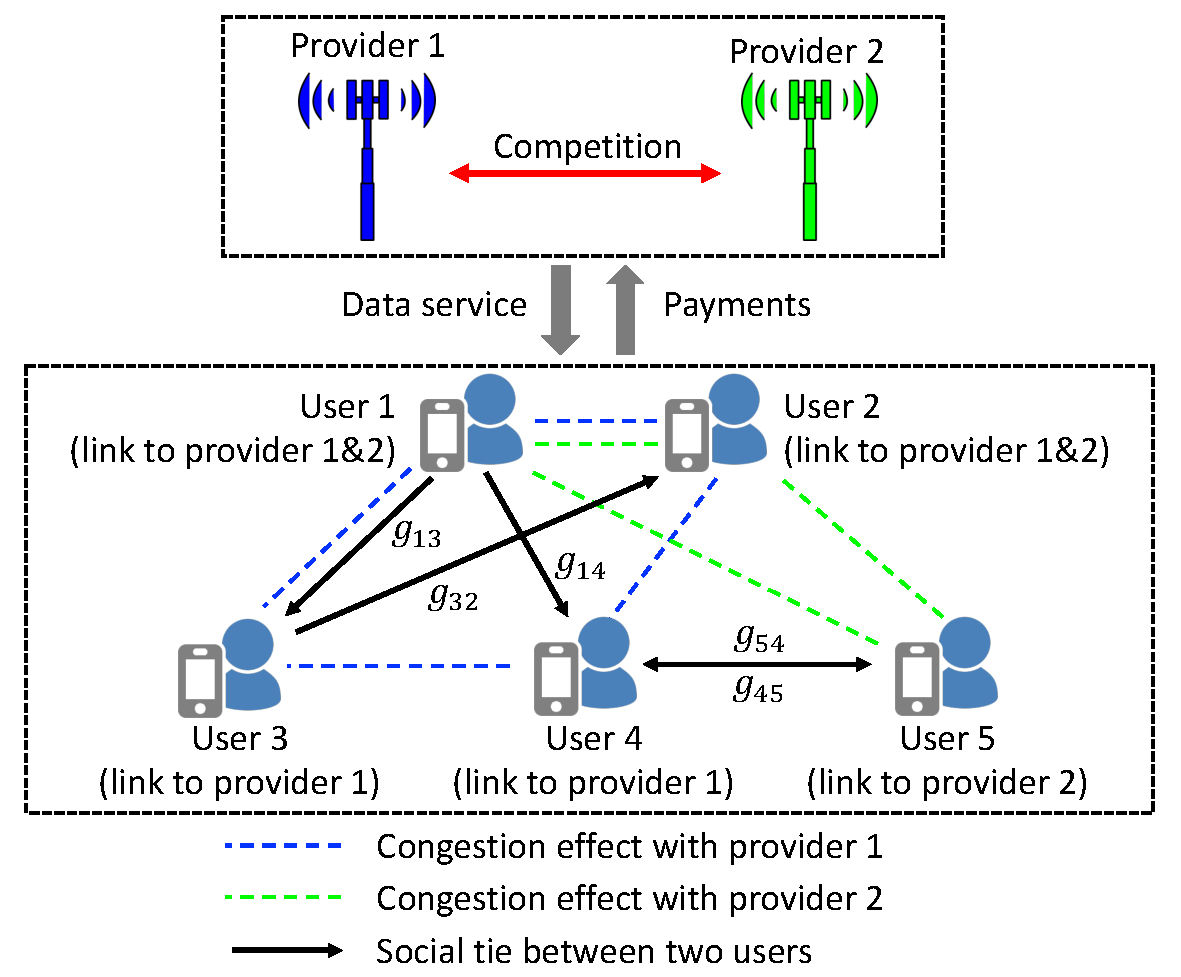
\includegraphics[scale=0.6]{./pic/scheme0.pdf}
\vspace{-0.0cm}
%\caption{An illustration of the system model and interactions among service providers and mobile users.}\label{fg:scheme}
\caption{系统模型以及服务提供商和移动用户之间的交互关系示意图。}\label{fg:scheme}
\end{figure}


\subsection{斯塔克伯格博弈建模}
在本节中,我们将提供商定价-用户数据使用的问题建模为一个两阶段的\emph{斯塔克伯格博弈}。服务提供商通过阶段\uppercase\expandafter{\romannumeral1}中的非合作博弈来确定其服务定价,而其定价策略是基于第二阶段子博弈中用户之间的子博弈所确定的。
%In this section, we cast the pricing-usage problem as a two-stage \emph{Stackelberg game} where service providers determine their pricing profiles via a non-cooperative game in stage I, based on the total data demands determined by mobile users via a subgame in stage II.
%The equilibrium of the game (if exists) would provide a satisfying solution in the sense that no one could be better off by unilaterally deviate from the equilibrium strategy.
%Specifically, in Stage I, given the pricing strategies of other providers, each provider determines the unit service price to maximize its revenue, and then announces the price to users. In Stage II, given the price from each  provider, each mobile user decides her data usage from each provider to maximize her individual utility. 
与文献[\citenum{GongDCZ17}]中考虑的垄断市场不同,在我们的案例中,每个移动用户的战略空间都是多维的,这给刻画用户博弈的均衡解增添了挑战。针对这一挑战,我们把联结一个移动用户和一个服务提供商的链接视为一个\emph{虚拟玩家},并将用户之间的数据使用问题视为虚拟玩家(链接)间的非合作博弈。我们令$\mathcal{L}\triangleq\{(i,k)\}_{i\in\N,k\in\K}$表示$L = N\times K$个链接的集合。虚拟玩家$(i,k)$的纯策略是指流经链接$(i,k)$的数据量$x^{k}_{i}$,而玩家$(i,k)$的收益对应于$u_{i}$(即始于同一用户的虚拟玩家具有相同的收益)。进而链接$(i',k')$对链接$(i,k)$的社交效应可以通过用户$i$和$i'$之间的社交联系量$g_{ii'}$来表征。我们令$\mathbf{x}=(\mathbf{x}_{1},\mathbf{x}_{2},\cdots,\mathbf{x}_{K})$表示所有链接上的数据使用量,并用$\mathbf{x}_{-(i,k)}$表示排除联结$(i,k)$后其他链接上的数据使用量。两阶段博弈的定义如下:
%Different from the monopoly market considered in \cite{GongDCZ17}, the strategy space of each mobile user in our case is multidimensional, making it more challenging to characterize the equilibrium of the usage game. To tackle this challenge, we treat the link connecting a mobile user and a provider as a \emph{virtual player}, and cast the data usage problem among users as a non-cooperative game played by virtual players (links). Let $\mathcal{L}\triangleq\{(i,k)\}_{i\in\N,k\in\K}$ denote the set of $L=N\times K$ user-provider links. The pure strategy of virtual player $(i,k)$ is the data usage $x^{k}_{i}$ over the link $(i,k)$ with its payoff corresponds to $u_{i}$ (i.e., the links starting from the same user have the same payoff). And it follows that the social network effect that link $(i',k')$ has on link $(i,k)$ can be characterized by the social tie $g_{ii'}$ between user $i$ and $i'$. We denote $\mathbf{x}=(\mathbf{x}_{1}, \mathbf{x}_{2},\cdots,\mathbf{x}_{K})$ as the joint link usage profile of all links, and use $\mathbf{x}_{-(i,k)}$ to denote the joint usage profile excluding $(i,k)$. And the two-stage game can be formally defined as follows:

\begin{df}[两阶段提供商定价-用户数据使用博弈]\label{def:mlmf}
\mbox{}
\begin{itemize}
    \item \emph{阶段\uppercase\expandafter{\romannumeral1}(提供商定价博弈 $\mathcal{G}_P\triangleq\{\K,\mathcal{P},\{v_k\}_{k\in\K}\}$):} \\
    在用户(链接)数据使用量为$\mathbf{x}$的情况下,给定其他提供商的定价策略$\mathbf{p}_{-k}$,每个提供商$k\in\K$选择$p_k$来最大化其收入$v_k$。定价博弈的均衡解可表示为一个联合定价策略$\mathbf{p}^*=(p^{*}_{1}\cdots,p^{*}_{K})$满足下式
    %Under the links' usage profile $\mathbf{x}$, each provider $k\in\K$ chooses $p_k$ to maximize its revenue $v_k$, given other providers' pricing strategies $\mathbf{p}_{-k}$. The pricing equilibrium is a joint pricing profile $\mathbf{p}^*=(p^{*}_{1}\cdots,p^{*}_{K})$ such that 
        \begin{equation}
          p^*_k=\arg\max_{p_k\in\mathcal{P}_k}v_k(p_k,\mathbf{p}^{*}_{-k},\mathbf{x}), ~\forall k\in\K.
        \end{equation}
        
    \item \emph{阶段\uppercase\expandafter{\romannumeral2}(用户数据使用博弈$\mathcal{G}_U\triangleq\{\mathcal{L},\mathbb{R}_+^L,\{u_i\}_{i\in\N}\}$):}\\
    给定提供商的定价策略$\mathbf{p}$和其他链接的数据使用量$\mathbf{x}_{-(i,k)}$,每个链接$(i,k)\in\mathcal{L}$选择从服务商$k$处使用量为$x^{k}_i$的服务以最大化其收益$u_ {i}$。用户数据使用博弈的均衡解可表示为$\mathbf{x^*}=(\mathbf{x}^*_{1},\mathbf{x}^*_{2},\cdots,\mathbf{x}^*_{K})$,这种情况下任何用户都无法通过单方面更改其使用量来增加其个人收益:
    %Given providers' pricing profile $\mathbf{p}$, each link $(i,k)\in\mathcal{L}$ chooses a usage demand $x^{k}_i$ to maximize her payoff $u_{i}$ given other links' usage profile $\mathbf{x}_{-(i,k)}$. The link demand equilibrium is a joint usage profile $\mathbf{x^*}=(\mathbf{x}^*_{1}, \mathbf{x}^*_{2},\cdots,\mathbf{x}^*_{K})$ such that no user can increase its payoff by unilaterally changing its usage profile:    
        \begin{equation}
          x^{k*}_i=\arg\max_{x^{k}_i\in \mathbb{R}_+}u_i(x^{k}_i,\mathbf{x}^*_{-(i,k)},\mathbf{p}), ~\forall i\in\N.
        \end{equation}
\end{itemize}
\end{df}

当博弈问题处于均衡解时任何参与博弈的玩家单方面偏离其均衡策略的行为都将导致其自身的收益降低。按照惯例,我们采用反向归纳法\cite{osborne}来分析斯塔克伯格博弈。我们首先来研究阶段\uppercase\expandafter{\romannumeral2}中的数据使用博弈。
%The equilibrium solution of the game (if exists) would provide a satisfying solution in the sense that any unilaterally deviation from the equilibrium solution would lead to a payoff degradation. By convention, we appeal to the backward induction approach\cite{osborne} to analyze the Stackelberg game. Next, we first study the usage game in Stage II. 

\section{用户数据使用博弈中的联结需求均衡}\label{sec:stageII}

在本节中,我们将在给定服务提供商定价策略的情况下研究提供商-用户链接的数据使用需求。根据公式(\ref{eq:userU})和一阶条件$\frac{\partial u_{i}}{\partial x^{k}_{i}} = 0$,我们获得了链接$(i,k)$的最佳响应函数为
%In this section, we study the usage demand over links given the joint pricing profile of service providers. Using function (\ref{eq:userU}) and the first-order condition, $\frac{\partial u_{i}}{\partial x^{k}_{i}}=0$, we obtain the best response function of link $(i,k)$ as
\begin{align}\label{br1}
%\small
\bold{B}^{k}_{i}\left(\mathbf{x}_{-(i,k)}\right)=&\max\left\{0,\frac{a_i-p_k}{b_i+c}-\frac{b_i\sum_{k'\neq k}x^{k'}_i}{b_i+c}\right.\nonumber\\
&\left.+\frac{\sum_{j\neq i}g_{ij}\sum_{m\neq k}x_{j}^{m}}{b_i+c}+\frac{\sum_{j\neq i}(g_{ij}-c)x_{j}^{k}}{b_i+c}\right\}.
\end{align}

根据(\ref{br1}),每个链接的最佳响应包括两部分:独立于其他链接的内在需求$\frac{a_i-p_k}{b_i + c}$,和取决于其他链接的外部需求$-\frac{b_i\sum_{k'\neq k}x^{k'}_i}{b_i + c} + \frac {\sum_{j\neq i}g_{ij}\sum_{m\neq k}x_{j}^{m}}{b_i + c} + \frac{\sum_{j\neq i}(g_{ij} -c)x_{j}^{k}}{b_i + c}$。具体来说,对于外部需求,第一项$-\frac{b_i \sum_{k'\neq k}x^{k'}_i}{b_i + c}$表征了其他同样始于用户$i$的链接对链接$(i,k)$的负面影响,这体现了使用除去提供商$k$以外的其他提供商的数据服务将削弱对于服务提供商$k$的数据使用。第二项$\frac{\sum_{j\neq i}g_{ij}\sum_{m\in\K}x_{j}^{m}}{b_i + c}$刻画了联结除用户$i$和提供商$k$的其他链接对于$(i,k)$所产生的正面网络外部性影响。第三项中的系数$\frac{g_{ij}-c}{b_i + c}$则刻画了与提供商$k$连接的其他链接对链接$(i,k)$上需求的边际影响。显然,如果社会效应主导了拥挤效应(即$g_{ij}\geq c$),则边际影响是正面的;而如果拥塞效应占主导地位(即$g_{ij} <c$),则边际影响为负面的。
%According to (\ref{br1}), the best response of each link consists of two parts: the internal demand, $\frac{a_i-p_k}{b_i+c}$, which is independent of other links, and the external demand, $-\frac{b_i\sum_{k'\neq k}x^{k'}_i}{b_i+c}+\frac{\sum_{j\neq i}g_{ij}\sum_{m\neq k}x_{j}^{m}}{b_i+c}+\frac{\sum_{j\neq i}(g_{ij}-c)x_{j}^{k}}{b_i+c}$, which depends on those links that are owned by the same user or are connected with the same service provider. Specifically, the first term $-\frac{b_i\sum_{k'\neq k}x^{k'}_i}{b_i+c}$ characterizes the negative effect on link $(i,k)$ from other links starting from user $i$, implying that the data usage from providers other than $k$ would dampen the usage from service provider $k$. The second term $\frac{\sum_{j\neq i}g_{ij}\sum_{m\in\K}x_{j}^{m}}{b_i+c}$ indicates the level of positive network effect on link $(i,k)$ from the links that connect user $i$'s social neighbors and service providers excluding $k$. The coefficient $\frac{g_{ij}-c}{b_i+c}$ characterizes the marginal impact on the demand of link $(i,k)$ from other links that also connect with provider $k$. Clearly, if the social effect dominates the congestion effect (i.e., $g_{ij}\geq c$), the marginal impact is positive; while if the congestion effect dominates (i.e., $g_{ij}<c$), the marginal impact is negative.

%\footnote{我们有$\forall i,i'\in\N$,如果$i<i'$,则\tau(i,k)<\tau(i',k)$;$\forall k,k'\in\K$,如果$k<k'$,则$\tau(i,k)<\tau(i,k')$。}


\subsection{联结需求均衡的存在性与唯一性}
我们首先讨论用户博弈中链接需求均衡的存在性。在不失一般性的前提下,我们仅关注数据使用量大于零的链接,而那些具有零使用量的链接在策略求解中是冗余的。令$\mathcal{L}^{+}$表示具有正数据使用量的链接集合,即$x^{k}_{i}> 0,\forall(i,k)\in\ca{L }^{+}$。我们定义$\tau:\ca{L}^{+}\rightarrow(1,2,\cdots,L^+)$为一个映射使得$\tau(i,k)$使用索引$l\in\{1,\cdots,L^+\}$\footnote{$\forall i,i'\in\N$,如果$i<i'$则$\tau(i,k)<\tau(i',k)$;$\forall k,k'\in\K$,如果$k<k'$,则$\tau(i,k)<\tau(i,k')$。}对链接$(i,k)\in\ca{L}^{+}$进行标记。为了方便起见,我们令$\mathbf{u}^+ =(u^{+}_{1},\cdots,u^{+}_{L^{+}})$表示效用向量,其中$u^{+}_{\tau(i,k)} = u_{i}$,$\mathbf{x}^{+} =(x^{+}_{1}, \cdots, x^{+}_{L^{+}})$表示使用向量,其中$x^{+}_{\tau(i,k)} = x^{k}_{i}$,$\mathbf{p}^+=(p^{+}_{1}, \cdots, p^{+}_{L^{+}})$表示价格向量,其中$p_{\tau(i,k)}^+ = p_k$表示链接$(i,k)$和$\mathbf{a}^+ =(a^{+}_{1}, \cdots, a^{+}_{L^{+}})$表示系数向量,其中$a_{\tau(i,k)}^+ = a_i$表示链接$(i,k)$的固有系数。我们通过图\ref{fg:layout}中的示例说明了注释规则,其中系统由三个服务提供商和四个移动用户组成。因此,我们有$L^+= |\mathcal{L}| = 9$,$\mathbf{a}^+=(a_1,a_1,a_1,a_2,a_2,a_3,a_3,a_3,a_4)$,和$\mathbf{p}^+=(p_1,p_1,p_1,p_2,p_2,p_3,p_3,p_3,p_4)$。
%We first discuss the existence of a link demand equilibrium for the usage game. Without loss of generality, we focus only on the links with positive usage, as those links with zero usage are strategically redundant to the network. Let $\mathcal{L}^{+}$ denote the set of links with positive data usage, i.e., $x^{k}_{i}>0,\forall (i,k)\in\ca{L}^{+}$, and define $\tau:\ca{L}^{+}\rightarrow(1,2,\cdots,L^+)$ as a mapping, such that $\tau(i,k)$ labels the link $(i,k)\in\ca{L}^{+}$ with an index $l\in\{1,\cdots,L^+\}$\footnote{In particular, we have $\tau(i,k)<\tau(i,k')$, if $k<k'$ and $\tau(i,k)<\tau(i',k)$, if $i<i'$, $\forall i,i'\in\N$, and $\forall k,k'\in\K$.}. For convenience, let $\mathbf{u}^+=(u^{+}_{1},\cdots,u^{+}_{L^{+}})$ denote the utility vector with $u^{+}_{\tau(i,k)}=u_{i}$, $\mathbf{x}^{+}=(x^{+}_{1},\cdots,x^{+}_{L^{+}})$ denote the usage vector with $x^{+}_{\tau(i,k)}=x^{k}_{i}$, $\mathbf{p}^+=(p^{+}_{1},\cdots,p^{+}_{L^{+}})$ denote the price vector with $p_{\tau(i,k)}^+=p_k$ indicating the service price on link $(i,k)$, and $\mathbf{a}^+=(a^{+}_{1},\cdots,a^{+}_{L^{+}})$ denote the coefficient vector with $a_{\tau(i,k)}^+=a_i$ representing the intrinsic coefficient of link $(i,k)$. We illustrate the notation rules via an example as shown in Fig. \ref{fg:layout}, where the system consists of three service providers and four mobile users. Accordingly, we have $L^+=|\mathcal{L}|=9$, $\mathbf{a}^+=(a_1,a_1,a_1,a_2,a_2,a_3,a_3,a_3,a_4)$, and $\mathbf{p}^+=(p_1,p_1,p_1,p_2,p_2,p_3,p_3,p_3,p_4)$.

\begin{figure}
\centering
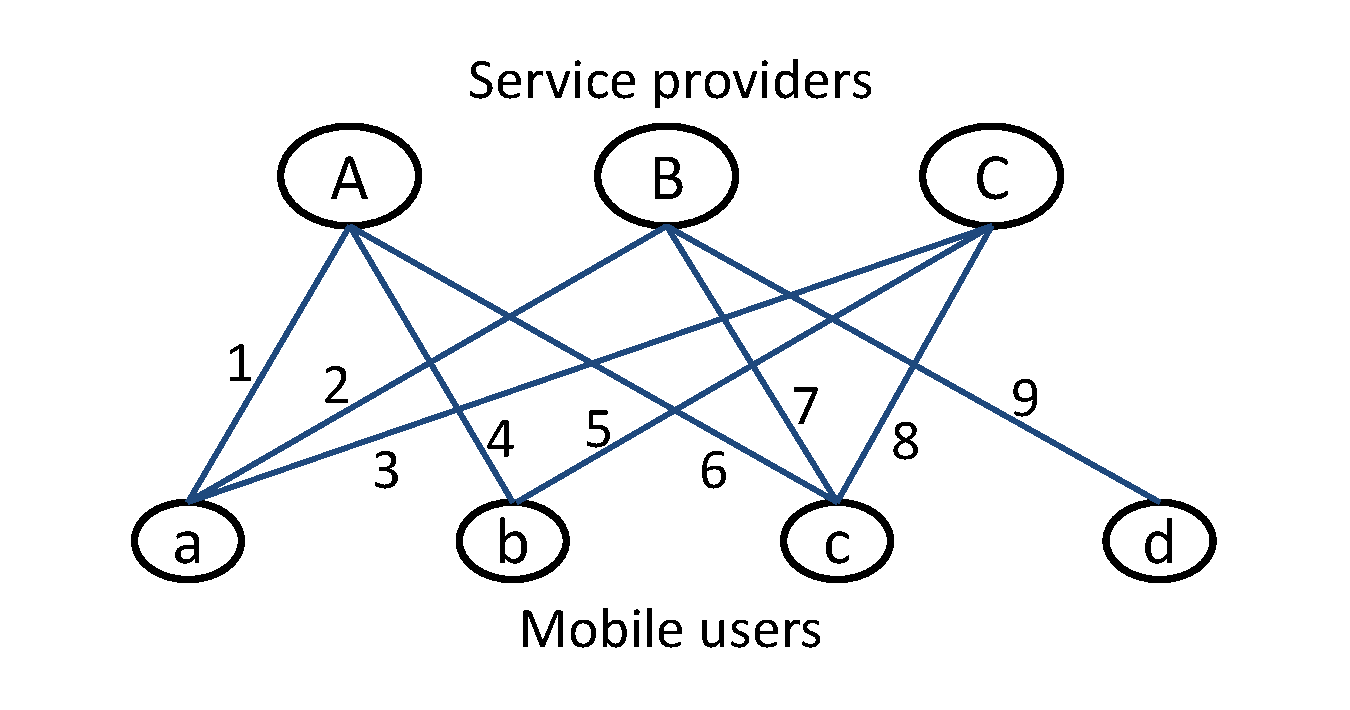
\includegraphics[scale=0.4]{./pic/layout.pdf}
%\caption{Illustration of a system with three service providers and four mobile users with nine positive usage links.}\label{fg:layout}
\caption{包含三个服务提供商和四个移动用户的系统示意图,系统中存在9条链接。}\label{fg:layout}
\end{figure}

接下来,我们通过引理\ref{lm:LCP}证明用户数据使用博弈$\ca{G}_U^{+}\triangleq(\mathcal{L}^+,\mathbb{R}_+^L,\{u_i\}_{i\in\N})$的链接需求均衡解是最佳响应函数(\ref{br1})所对应的以下线性互补问题(LCP)\cite{lcp}的解。
%In the sequel, we show that all the link demand equilibria of the usage game $\ca{G}_U^{+}\triangleq(\mathcal{L}^+,\mathbb{R}_+^L,\{u_i\}_{i\in\N})$ are the solutions to the following linear complementarity problem (LCP)\cite{lcp} formed based on the best response function (\ref{br1}), as presented in Lemma \ref{lm:LCP}. 


\begin{lm}\label{lm:LCP}

给定价格向量$\mathbf{p}^{+}$,联合数据使用量$\mathbf{x}^{+*}\in\mathbb{R}^{L^+}_+$是博弈$\ca{G}_U^{+}$的一个链接需求均衡当且仅当$\mathbf{x}^{+*}$是如下定义的线性互补性问题$LCP(W,\mathbf{x}^{+})$的解:
%Given price vector $\mathbf{p}^{+}$, a joint usage profile $\mathbf{x}^{+*}\in\mathbb{R}^{L^+}_+$ is a link demand equilibrium of game $\ca{G}_U^{+}$, if and only if $\mathbf{x}^{+*}$ is the solution to the linear complementarity problem $LCP(W,\mathbf{x}^{+})$ defined by the following inequalities:
\begin{equation}\label{eq:LCP}
%\small
\begin{cases}
    \mathbf{x}^{+}>0\\
    \mathbf{a}^{+}-\mathbf{p}^{+}-W\mathbf{x}^{+}\leq 0\\
    (\mathbf{x}^{+})^T(\mathbf{a}^{+}-\mathbf{p}^{+}-W\mathbf{x^{+}})=0
\end{cases},
\end{equation}
\noindent 其中$W$是$L^+\times L^+$维的加权邻接矩阵,其中位于$\tau(i,k)$行$\tau(i',k')$列中的元素定义为如下:
%\noindent where $W$ is a $L^+\times L^+$ weighted adjacency matrix with the element at row $\tau(i,k)$ and column $\tau(i',k')$ defined as follows:
\begin{equation}
%\small
w_{\tau(i,k),\tau(i',k')}=
\begin{cases}
  b_i+c,~~~&\mbox{if $i=i', k=k'$};\\
  b_i,~~~&\mbox{if $i=i', k\neq k'$};\\
  c-g_{ii'},~~~&\mbox{if $i\neq i', k=k'$};\\
  -g_{ii'},~~~&\mbox{if $i\neq i', k\neq k'$}.
\end{cases}
\end{equation}
\end{lm}

首先,我们声明用户数据使用博弈存在一个链接需求均衡解。
%Firstly, we claim the existence of a link demand equilibrium for the usage game.

\begin{thm}
对于用户数据使用博弈$\ca{G}_U^+$存在至少一个链接需求平衡$\mathbf{x}^{+*}$。
 % The existence of a link demand equilibrium $\mathbf{x}^{+*}$ is guaranteed for the link usage game $\ca{G}_U^+$.
\end{thm}
上述定理的证明并不复杂。由于一组链接的最佳响应定义了一个从凸紧致欧氏子空间到自身的映射,因此我们可以使用Brouwer不动点定理证明链接需求均衡的存在。 
%The proof is straightforward given the fact that the set of link best responses defines a continuous mapping from a convex compact subset of a Euclidean space into itself, based on which we can use Brouwer's fix-point Theorem to demonstrate the existence of a link demand equilibrium.


接下来,基于引理\ref{lm:LCP},我们来证明在以下条件下链路需求均衡的唯一性。
%Next, based on Lemma \ref{lm:LCP}, we show the uniqueness of the link demand equilibrium under the following conditions.


\begin{thm}\label{thm:unique}
矩阵$W$在满足对角优势条件情况下,即$\forall(i,k)\in\ca{L}$,
 % Under the diagonal dominance condition of matrix $W$, that is, $\forall (i,k)\in\ca{L}$, 
\begin{equation}\label{eq:condition}
  \begin{cases}
  %\small
  w_{(\tau(i,k),\tau(i,k))}\geq\sum_{(i',k')\in\ca{L}/(i,k)}|w_{\tau(i,k),\tau(i',k')}|, \\
  w_{(\tau(i,k),\tau(i,k))}\geq\sum_{(i',k')\in\ca{L}/(i,k)}|w_{\tau(i',k'),\tau(i,k)}|,
  \end{cases}
 \end{equation}
 用户数据使用博弈$\ca{G}_U^+$存在以下唯一的链接需求均衡,
% the link usage game $\ca{G}_U^+$ admits a unique link demand equilibrium, given by
  \begin{equation}\label{eq:LDE}
  	\mathbf{x}^{+*}=W^{-1}(\mathbf{a}^{+}-\mathbf{p}^{+}).
  \end{equation}
\end{thm}
\begin{proof}
为了证明链接需求均衡的唯一性,我们证明用户数据使用博弈$\ca{G}_U^+$在满足条件(\ref{eq:condition})的情况下属于凹博弈。收益函数$\mathbf{u}^+(\mathbf{x})$ 的雅克比矩阵$\nabla\mathbf{u}^+(\mathbf{x})$ 如下所示, 
\begin{equation}
\begin{array}
[c]{lll}%
\mathbf{X}&=
  \begin{bmatrix}
   \frac{\partial^2u_1^+(\mathbf{x}^+)}{{\partial x^{+}_1}^2}  &  \frac{\partial^2u_1^+(\mathbf{x}^+)}{\partial x^{+}_1\partial x^{+}_2}  &  ~\cdots  &  \frac{\partial^2u_1^+(\mathbf{x}^+)}{\partial x^{+}_1\partial x^{+}_{L^+}}\\
   \frac{\partial^2u_2^+(\mathbf{x}^+)}{\partial x^{+}_2\partial x^{+}_1}  &  \frac{\partial^2u_1^+(\mathbf{x}^+)}{{\partial x^{+}_2}^2}  &  ~\cdots  &  \frac{\partial^2u_2^+(\mathbf{x}^+)}{\partial x^{+}_2\partial x^{+}_{L^+}}\\
    \vdots  &  \vdots  &  ~\ddots  &  \vdots\\
   \frac{\partial^2u_{L^+}^+(\mathbf{x}^+)}{\partial x^{+}_{L^+}\partial x^{+}_1}  &  \frac{\partial^2u_{L^+}^+(\mathbf{x}^+)}{\partial x^{+}_{L^+}\partial x^{+}_2}  &  ~\cdots  &  \frac{\partial^2u_{L^+}^+(\mathbf{x}^+)}{{\partial x^{+}_{L^+}}^2}\\
  \end{bmatrix}\\[45pt]  
  &=-W
\end{array}
\end{equation}
在条件(\ref{eq:condition})的情况下,矩阵$W$即满足行对角占优同时也满足列对角占优,同时其转置$W^T$也是对角占优的。于是我们有
\begin{equation}
 \nabla\mathbf{u}^+(\mathbf{x}) + \nabla\mathbf{u}^+(\mathbf{x})^T = -W - W^T
\end{equation}
是严格对角占优且对称的。根据文献\cite{Horn85}中的现有结论,当一个严格对角占优对称矩阵的对角元素为非负实数时,该矩阵为正定的。因此在这里,我们有$\nabla\mathbf{u}^+(\mathbf{x}) + \nabla\mathbf{u}^+(\mathbf{x})^T$是负正定的矩阵。依据文献\cite{econometrica}中的定理,我们可以得到$\nabla\mathbf{u}^+(\mathbf{x})$是严格对角凹的。因此,利用文献\cite{econometrica}中定理2的结果,我们可以得到博弈$\ca{G}_U^+$ 存在唯一的链接需求均衡。
\end{proof}
定理\ref{thm:unique}的证明基于以下事实:在条件\ref{eq:condition}下,式(\ref{eq:LCP})所定义的线性互补问题$LCP(W,\mathbf{x}^{+})$对应于一个凹博弈(Concave game),因此解$\mathbf{x}^{+*}$是唯一的。基于引理\ref{lm:LCP}所述的,即问题$LCP(W,\mathbf{x}^{+})$的解与博弈$\ca{G}_U^{+}$的均衡点对应,我们可据此确定链接需求均衡点在特定条件下的唯一性。详细的证据参见附录A。正如(9)所示,我们可以显式地将链接需求均衡点表述为$\mathbf{a}^{+}$和$\mathbf{p}^{+}$的线性组合。因此,当达到链接需求均衡点时每名用户$i\in\N$的使用消耗量$\sum_{k\in\K}x^{+*}_{\tau(i,k)}$应是$\mathbf{a}=(a_1,\cdots,a_N)$和$\mathbf{p}=(p_1,\cdots,p_K)$的线性函数。

%The proof of Theorem \ref{thm:unique} follows from the fact that under the condition (\ref{eq:condition}), the linear complementarity problem $LCP(W,\mathbf{x}^{+})$ defined in (\ref{eq:LCP}) corresponds to a concave game, thus has a unique solution $\mathbf{x}^{+*}$. Since the solution of problem $LCP(W,\mathbf{x}^{+})$ corresponds to the equilibrium of the game $\ca{G}_U^{+}$ as indicated by Lemma \ref{lm:LCP}, we can thereby establish the conditional uniqueness of the link demand equilibrium. The detailed proof has been relegated to the Appendix A. As shown in (\ref{eq:LDE}), we can explicitly express the link usage equilibrium as a linear combination of $\mathbf{a}^{+}$ and $\mathbf{p}^{+}$. As a result, the usage consumption of each user $i\in\N$ under the link demand equilibrium, $\sum_{k\in\K}x^{+*}_{\tau(i,k)}$, should be a linear function of $\mathbf{a}=(a_1,\cdots,a_N)$ and $\mathbf{p}=(p_1,\cdots,p_K)$. 

\section{理性服务提供商之间的定价博弈}\label{sec:stageI}
%\section{Pricing Game among Rational Service Providers}\label{sec:stageI}
在上一节中,我们已经说明了阶段\uppercase\expandafter{\romannumeral2}数据使用博弈存在链接需求均衡点并且均衡点具有唯一性。接下来,我们来说明第一阶段无线提供商服务价格的确定。从理论上讲,每个服务提供商都可以在一个连续的价格变量上优化其收入。实际上,服务提供商宣布的价格通常落在离散样本空间内,并在一组离散价格水平上服从指定概率分布。为了刻画这个特征,在我们所关注的定价博弈中,服务提供商针对其他用户的策略通过选择概率定价策略来最大化其期望收入。在本节中,我们考虑传统的情况,即理性的服务提供商客观地评估自己的收入和其他用户的策略。我们确定了博弈混合策略定价均衡点的存在性。
%In the previous section, we have shown the existence and uniqueness of the link demand equilibrium for the usage game in Stage II. Next, we move on to the determination of service prices for wireless providers in Stage I. Theoretically, each service provider can optimize his revenue over a continuous price variable. While in practice, the price announced by the service provider usually falls within a discrete sample space with a probabilistic distribution specified over a set of discrete price levels. To capture this feature, our discussion focuses on the pricing game that service providers maximize their expected revenues via choosing probabilistic pricing strategies against other users' strategies. In this section, we consider the conventional scenario where rational service providers evaluate their own revenue and other users' strategies objectively. We establish the existence of a mixed-strategy pricing equilibrium for the game. 

\subsection{混合策略定价均衡点的存在性}\label{sec:exist1}
我们将提供商$k$的混合策略定义为$\pi_{k}=(\pi_k(p_{k}^1),\pi_k(p_{k}^2),\cdots,\pi_k(p_{k}^{M_{k}}))\in\Delta \mathcal{P}_{k}$, 其中$\pi_k(p_{k}^m)\in[0,1]$是提供者$k$选择价格$p_{k}^m\in\mathcal{P}_k$的概率。既而我们有$\sum_{m=1}^{M_k}\pi_k\left(p_{k}^{m}\right)=1$。我们定义一个联合的混合策略定价策略$\pi=(\pi_{1},\cdots,\pi_{K})$为一个笛卡尔积$\Delta \mathcal{P}\triangleq\prod_{k\in\K} \Delta \mathcal{P}_{k}$。遵循冯·诺依曼·摩根斯坦恩的期望效用理论(EUT)\cite{Von},在混合策略下,提供商$k\in\K$的收入$z_k^{EUT}$可以表示为
%We define the mixed-strategy of provider $k$ as $\pi_{k}=(\pi_k(p_{k}^1),\pi_k(p_{k}^2),\cdots,\pi_k(p_{k}^{M_{k}}))\in\Delta \mathcal{P}_{k}$, where $\pi_k(p_{k}^m)\in[0,1]$ is the probability that provider $k$ chooses price $p_{k}^m\in\mathcal{P}_k$, with $\sum_{m=1}^{M_k}\pi_k\left(p_{k}^{m}\right)=1$. A joint mixed-strategy pricing profile $\pi=(\pi_{1},\cdots,\pi_{K})$ is defined as a joint probability distribution over the Cartesian product $\Delta \mathcal{P}\triangleq\prod_{k\in\K} \Delta \mathcal{P}_{k}$. Following Von Neumann-Morgenstern's Expected Utility Theory (EUT) \cite{Von}, the revenue of a provider $k\in\K$ under mixed strategies, denoted by $z_k^{EUT}$, can be written as
\begin{equation}\label{eq:EUT}
%\small
z_{k}^{EUT}(\pi_{k},\pi_{-k})=\sum_{\mathbf{p}\in \mathcal{P}}\left(\prod_{k\in\K}\pi_k(p_{k})\right)v_k,
\end{equation}
其中$\pi_{-k}\in\prod_{k'\in\K,k'\neq k}\Delta\mathcal{P}_{k'}$表示除提供商$k$外的所有其他提供商的混合策略。这里,$v_k$可以根据(\ref{eq:SPrev})计算得到,其中总数据使用量从阶段\uppercase\expandafter{\romannumeral2}的链路需求均衡$\mathbf{x}^{+*}$获得(如上节\ref{sec:stageII}所述)。
%where $\pi_{-k}\in\prod_{k'\in\K,k'\neq k}\Delta\mathcal{P}_{k'}$ denotes the mixed strategies of all other providers except provider $k$. Here, $v_k$ can be calculated according to (\ref{eq:SPrev}), in which the aggregated consumption is obtained from the link demand equilibrium $\mathbf{x}^{+*}$ of Stage I (as discussed in Section \ref{sec:stageII}).

我们根据期望效用理论将定价博弈重新定义为$\mathcal{G}_P^{EUT}\triangleq(\mathcal{K},\Delta\mathcal{P},\{z^{EUT}_k\}_{k\in\mathcal{K}})$。定价博弈的混合策略纳什均衡定义如下。
%We redefine the pricing game under Expected Utility Theory as $\mathcal{G}_P^{EUT}\triangleq(\mathcal{K},\Delta\mathcal{P},\{z^{EUT}_k\}_{k\in\mathcal{K}})$. The mixed-strategy Nash equilibrium for the pricing game is defined as follows.

\begin{df}[混合价格策略均衡]
我们认为如果对于每个服务提供商$k\in\mathcal{K}$,以下条件满足
%The mixed-strategy pricing profile $\pi^*=(\pi_{1}^*,\cdots,\pi_{K}^*)\in\Delta\mathcal{P}$ is a mixed-strategy pricing equilibrium, if for every service provider $k\in\mathcal{K}$, we have
\begin{equation}\label{eq:exrev1}
z_{k}(\pi_{k}^*,\pi_{-k}^*)\ge z_{k}(\pi_{k},\pi_{-k}^*),~\forall \pi_k\ne\pi_k^*.
\end{equation}
则混合定价策略$\pi^*=(\pi_{1}^*,\cdots,\pi_{K}^*)\in\Delta\mathcal{P}$是一个混合策略价格均衡。
\end{df}

在下面的定理中,我们说明了博弈$\mathcal{G}^{EUT}_{P}$中存在混合策略定价均衡。
%In the following Theorem, we show the existence of a mixed-strategy pricing equilibrium for the game $\mathcal{G}^{EUT}_{P}$.
\begin{thm}\label{thm:exist}
定价博弈$\mathcal{G}^{EUT}_{P}$至少存在一个混合策略的定价均衡$\pi^{*}\in\Delta\mathcal{P}$。
%There exists at least one mixed-strategy pricing equilibrium $\pi^{*}\in\Delta\mathcal{P}$ for the pricing game $\mathcal{G}^{EUT}_{P}$.
\end{thm}
\begin{proof}
根据我们的模型,每个无线服务提供商$k\in\K$会从$M_k$个价格中选择并进行定价。由于服务提供商的数量和每个服务提供商的定价策略空间都是有限的,因此定价游戏$\mathcal{G}^{EUT}_{P}$属于有限博弈。而混合策略定价均衡$\pi^*$是最佳响应对应(Best response correspondence)的固定点。根据Kakutani不动点定理,价格博弈$\mathcal{G}^{EUT}_{P}$至少存在一个混合策略的纳什均衡\cite{osborne}。
%According to our model, each wireless service providers $k\in\K$ sets the price from $M_k$ pricing strategies. Since both the number of service providers and the pricing strategy space of each service provider are finite, the pricing game $\mathcal{G}^{EUT}_{P}$ falls into the class of finite game. A mixed-strategy pricing equilibrium $\pi^*$ is a fixed point of the best-response correspondence. By the Kakutani's fixed point theorem, the existence of at least one mixed-strategy Nash equilibrium is guaranteed for the pricing game $\mathcal{G}^{EUT}_{P}$\cite{osborne}.
\end{proof}

在实际中,为了避免收敛时间慢和寻找平衡点所需的不必要开销,我们可以考虑落在混合策略纳什平衡点附近足够小邻域内的近似平衡点。我们因此定义以下$\epsilon$价格均衡:
%In practice, to avoid slow convergence time and unnecessary overhead of finding equilibria, we can consider approximate equilibrium solutions that fall within a small enough neighborhood of the mixed-strategy Nash Equilibrium. Consider an $\epsilon$-pricing equilibrium defined as follows:
\begin{df}[$\epsilon$-价格均衡]
如果对于每个服务提供商$k\in\mathcal{K}$,我们有
%A mixed-strategy pricing profile $\pi^*=(\pi_{1}^*,\cdots,\pi_{K}^*)\in\Delta\mathcal{P}$ is an $\epsilon$-pricing equilibrium, if for each service provider $k\in\mathcal{K}$, we have
\begin{equation}\label{approxNE}
%\small
z_{k}(\pi_{k}^*,\pi_{-k}^*)\ge z_{k}(\pi_{k},\pi_{-k}^*) + \epsilon,~\forall \pi_k\ne\pi_k^*.
\end{equation}
则混合策略定价均衡$\pi^*=(\pi_{1}^*,\cdots,\pi_{K}^*)\in\Delta\mathcal{P}$是一个$\epsilon$定价均衡。
\end{df}
由定理\ref{thm:exist},我们可以直接得出$\epsilon$定价平衡的存在性。为了明确地寻找一个$\epsilon$定价均衡,我们可以诉诸于论文\cite{MYCISS16}中第五节中提出的集中式算法。
%The existence of an $\epsilon$-Pricing Equilibrium follows directly from Theorem \ref{thm:exist}. To explicitly search for an $\epsilon$-pricing equilibrium, we can resort to a centralized algorithm proposed in Section V of our previous paper \cite{MYCISS16}.

%\section{Pricing Game among Service Providers with Bounded Rationality}\label{sec:stageI2}
\section{有限理性服务提供商之间的定价博弈}\label{sec:stageI2}
在第五节中,服务提供商的收入是基于期望效用理论建模的,其前提假设是完全理性的提供商在价格竞争中采取客观的行为。但是我们观察到,卖方在实践中的行为通常偏离经典的期望效用理论\cite{Kahneman}所预测的理性行为路径。具体来说,服务提供商可能会对其对手的概率定价策略以及自己的收益函数进行主观评估。我们使用展望理论(PT)来捕捉定价博弈中的行为因素。
%In Section V, service provider's revenue is modeled based on Expected Utility Theory assuming fully rational providers acting objectively during the pricing competition. However, it has been observed that, sellers' behavior in practice usually deviate from the rational path predicted by this classic Expected Utility Theory \cite{Kahneman}. Specifically, service providers may have subjective evaluation on the probabilistic pricing strategy of their opponents as well as their own revenue functions, which are used for decision making. In order to capture such behavioral factors in our proposed pricing game, we resort to Prospect Theory (PT).

\subsection{前景理论下的提供商收入期望}
%\subsection{Provider's Expected Revenue under Prospect Theory}

我们考虑前景理论的两个主要特征。第一个是\emph{概率失真效应},指现实中决策者倾向于看重小概率事件,但是看轻中等和大概率事件。
%具体而言,这种特性可以通过将客观概率$p$映射到主观概率的概率失真函数$w(p)$来刻画。
我们考虑同类服务提供商并使用较为广泛的概率失真函数有Prelec函数\cite{Prelec}。则
%We consider two main features of Prospect Theory. The first one is the \emph{probability distortion effect}, which states that decision maker is prone to overweigh events with small probability, but underweight medium and large probability events. Specifically, this characteristic can be captured by a probability distortion function $w(p)$ that maps an objective probability $p$ to a subjective one. A widely used probability distortion function is the Prelec function \cite{Prelec}:
%\begin{equation}\label{eq:distortion}
%w(p)=\exp(-(-\ln p)^{\alpha}), 0<\alpha\leq 1,
%\end{equation}
%其中$p$是事件的真实概率,$\alpha$是概率失真参数,$w(p)$是对应的主观概率。图\ref{fg:dist_func}阐明了具有不同参数的概率失真函数(\ref{eq:distortion})。我们可以看到所有曲线在点$1/e$相交。此外,当$0\leq p < 1/e$时,函数是凸的,$w(p)<p$(即低估客观概率);而当$1/e\leq p<1$时,函数是凹的,我们有$w(p)\geq p$(即高估客观规律)。失真参数$\alpha$的值越小,则概率失真效应越明显。当$\alpha$设置为1时,该函数即变为客观概率。
提供商的主观评估可以通过式(\ref{eq:distortion})中给出的具有相同$\alpha$取值的失真函数来表征。同时,我们假设服务提供商能够客观地评估自身的策略。因而在前景理论下,用户$k$对联合定价策略$\mathbf{p}\in\Delta\mathcal{P}$的评估可以表示为$\pi_k(p_k)w(\prod_{k'\in\K,k'\neq k}\pi_{k'}(p_{k'}))$。
%where $p$ is the real probability of an event, $\alpha$ is the probability distortion parameter, and $w(p)$ is the corresponding subjective probability. Fig. \ref{fg:dist_func} illustrates the probability distortion function (\ref{eq:distortion}) with different parameters. We can see that all the curves intersect at the point $1/e$. Besides, we have when $0\leq p < 1/e$, the function is convex, and $w(p)<p$ (under-weighting); when $1/e\leq p<1$, the function is concave, and we have $w(p)\geq p$ (over-weighting). A smaller value of distortion parameter $\alpha$ corresponds to a more significant probability distortion effect. When $\alpha$ is set to 1, the function reduces to the objective probability. In our work, we consider homogeneous service providers whose subjective evaluation can be characterized by the distortion function given in (\ref{eq:distortion}) with a same fixed value of $\alpha$. Meanwhile, we assume that service providers are able to evaluate their own strategies objectively. Thus, user $k$'s evaluation for a joint pricing strategy $\mathbf{p}\in\Delta\mathcal{P}$ under Prospect Theory can be expressed as $\pi_k(p_k)w(\prod_{k'\in\K,k'\neq k}\pi_{k'}(p_{k'}))$.
%\begin{figure}
%\centering
%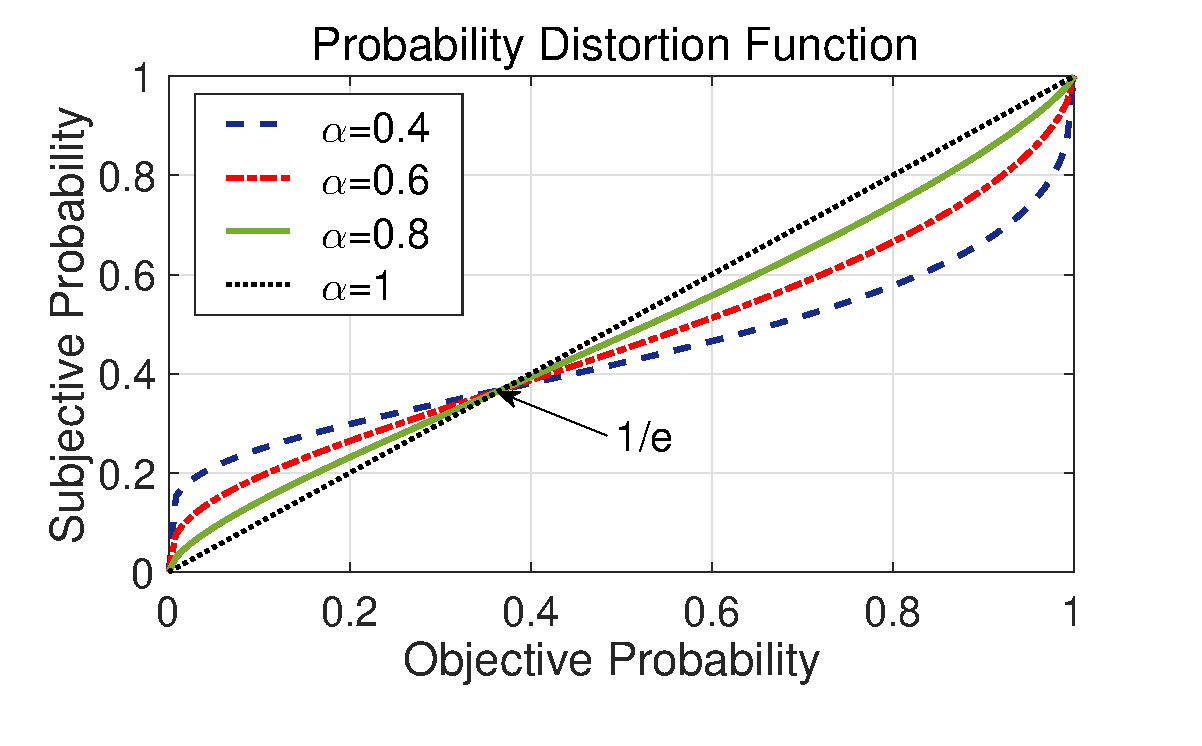
\includegraphics[scale=0.58]{./pic/dist_func.eps}
%%\caption{Probability distortion functions under different distortion parameters $\alpha$.}\label{fg:dist_func}
%\caption{失真参数$\alpha$不同取值下的概率失真函数。}\label{fg:dist_func}
%\vspace{0.1cm}
%\centering
%\includegraphics[scale=0.58]{./pic/fram_func.eps}
%%\caption{Framing functions under different utility aversion parameters $\beta$ and loss penalty parameter $\lambda$.}\label{fg:fram_func}
%\caption{不同效用规避参数$\beta$和损失惩罚参数$\lambda$下的框架函数。}\label{fg:fram_func}
%\end{figure}

我们考虑的前景理论的另一个特征是\emph{效用框架效应}。此效应反映了每个服务提供商对自己的收益进行主观评估的实际情况。
%实际中,仅当其收入超过参照点$R$($R$无需等于零)时,每名用户才会将其视为收益增益,否则将视为收益损失。同样,在给定参考点$R$的情况下,S型单调框架函数$f(\cdot)$会进一步调整客观收入,其中函数在$v>R$侧为凹函数,而在$v<R$一侧是凸函数。此外,在$R$附近,收益损失比收益增益增长得更快,表明收益损失的边际效用大于收益增益的边际效用。
在本文中,我们使用基于Kahneman提出的框架函数\cite{Kahneman},
%Another characteristic of Prospect Theory we considered is the \emph{utility framing effect}. This effect captures the practical situation where each service provider has subjective evaluation of her own payoff. In practice, each user might consider her payoff as a gain only if it is above a reference point $R$ (not necessarily equals zero), and consider it as a loss otherwise. Also, given the reference point $R$, the objective payoff is further tuned by a S-shaped monotone framing function $f(\cdot)$, which is concave at the side where $v>R$, and convex at the side where $v<R$. In addition, in the neighborhood of $R$, the losses loom larger than gains indicating that the marginal utility in losses is larger than in gains. In this work, we use a framing function based on the one proposed in \cite{Kahneman},
%\begin{equation}\label{eq:framing}
%f(x;R)=
%\begin{cases}
%(v - R)^{\beta}, &v\geq R\\
%-\lambda(R-v)^{\beta}, &v<R
%\end{cases}
%\end{equation}
%其中参数$0<\beta\leq 1$和$\lambda\geq 1$分别用于刻画风险规避和损失规避的因素。图\ref{fg:fram_func}展示了不同参数取值下的框架函数。特别地,当博弈参与者收入远离参照点时,$\beta$值越大,表示风险规避程度较小;$\lambda$值的增大则刻画了博弈参与者在客观上经历等同的收益的损失和增益时,所主观上体验到的损失要大于所体验到的增益。容易看出,当$\beta=\lambda=1$时,主观收益曲线与原始的客观收益曲线一致。我们假设每个服务提供商$k$基于式(\ref{eq:framing})来评估其收入。
则在前景理论模型下,服务提供商$ k\in\K$的预期收入$z_k^{PT}$可写为
%where the parameters $0<\beta\leq 1$ and $\lambda\geq 1$ model the risk aversion and loss aversion respectively. Fig. \ref{fg:fram_func} illustrates the framing function with different parameters. In particular, a larger $\beta$ characterizes less degree of risk aversion when the player's payoff is away from the reference point; and a larger $\lambda$ captures the greater loss experienced by the player with her payoff being reduced by a certain amount, in comparison to the corresponding gain she experiences with the same amount of the payoff increase. It is easy to see that when $\beta=\lambda=1$, the subjective payoff boil down to the original objective payoff. We assume each service provider $k$ evaluate her revenue using (\ref{eq:framing}) with parameter $\beta_k$, and reference point $R_k, \forall k\in\K$. Under Prospect Theory model, the expected revenue $z_k^{PT}$ of service provider $k\in\K$ can be written as

\begin{equation}\label{eq:PT}
%\small
z_{k}^{PT}(\pi_{k},\pi_{-k})=\sum_{\mathbf{p}\in \mathcal{P}}\pi_k(p_k)w\left(\prod_{k'\in\K,k'\neq k}\pi_{k'}(p_{k'})\right)f_k(v_k).
\end{equation}

我们将前景理论讨论下的定价博弈表示为$\mathcal{G}_P^{PT}\left(\mathcal{K},\Delta\mathcal{P},\{z_k^{PT}(R_k)\}_{k\in\mathcal{K}}\right)$,并在下一节中重新讨论价格博弈的均衡解的存在。
%We denote the pricing game under Prospect Theory as $\mathcal{G}_P^{PT}\left(\mathcal{K},\Delta\mathcal{P},\{z_k^{PT}(R_k)\}_{k\in\mathcal{K}}\right)$, and revisit the existence of equilibrium solution for the pricing game in the next section.


\subsection{混合策略定价均衡点的存在性}
在节\ref{sec:exist1}中建立混合策略纳什均衡的存在时,概率上期望收入(\ref{eq:EUT})的线性性起着关键作用。然而正如前一节所述,在前景理论中参与者对通过非线性失真函数建模的信念进行主观加权。因此,我们需要重新评估游戏定价均衡的存在。我们首先对前景理论下的混合策略纳什均衡给出以下定义。
%The mixed-strategy Nash equilibrium requires players optimally choosing their strategies given their beliefs of other players' strategies. The linearity of expected revenue (\ref{eq:EUT}) in probabilities plays a key role in establishing the existence of a mixed-strategy Nash equilibrium. However, as mentioned in the previous section, players will subjectively weight their beliefs modeled via non-linear distortion function on the probabilities under Prospect Theory. Thus, we need to reevaluate the existence of the pricing equilibrium of the game. We first provide the following definition for the mixed-strategy Nash equilibrium under Prospect Theory.

\begin{df}[前景理论(PT)下的混合策略价格均衡]
如果对于每个服务提供商$k\in\mathcal{K}$有,
%We call a mixed-strategy profile $\pi^*=(\pi_{1}^*,\cdots,\pi_{K}^*)\in\Delta\mathcal{P}$ a mixed-strategy pricing equilibrium under Prospect Theory, if for each service provider $k\in\mathcal{K}$,
\begin{equation}
%\small
z_{k}^{PT}(\pi_{k}^*,\pi_{-k}^*)\geq z_{k}^{PT}(\pi_{k},\pi_{-k}^*),~\forall \pi_k\ne\pi_k^*.
\end{equation}
则我们称该混合价格策略$\pi^*=(\pi_{1}^*,\cdots,\pi_{K}^*)\in\Delta\mathcal{P}$为前景理论下的混合策略定价均衡。
\end{df}

我们在以下定理中证明,当每个服务提供商的参考点固定时,我们的定价博弈$\mathcal{G}_{P}^{PT}$存在混合纳什均衡。
%We show in the following Theorem that our pricing game $\mathcal{G}_{P}^{PT}$ admits a mixed Nash equilibrium under the condition that each service provider's reference point is fixed.
\begin{thm}\label{thm:exist2}
如果服务提供商的参考点$\{R_k\}_{k\in\mathcal{K}}$都是固定的,则定价博弈$\mathcal{G}^{PT}_{P}$存在至少一个混合策略均衡点$\pi^{*}\in\Delta\mathcal{P}$。
%At least one mixed-strategy pricing equilibrium $\pi^{*}\in\Delta\mathcal{P}$ is guaranteed for the pricing game $\mathcal{G}^{PT}_{P}$, if service providers' reference points $\{R_k\}_{k\in\mathcal{K}}$ are all fixed.
\end{thm}
\begin{proof}
对于每个$k\in\mathcal{K}$,给定任意$R_k\in \mathbb{R}$和$\pi_{-k}\in\Delta\mathcal{P}_{-k}$,对于每个价格$p_k\in\mathcal{P}_k$,期望收入$z_{k}^{PT}(\pi_k, \pi_{-k})$是$\pi_k(p_k)$的线性函数。由于$\Delta\mathcal{P}_{k}$是紧凑集合,因此最佳响应策略集$\bold{B}_k(\pi_{-k})\triangleq\{\pi'_k\in\Delta\mathcal{P}:z_{k}^{PT}(\pi'_k, \pi_{-k})\geq z_{k}^{PT}(\pi_k, \pi_{-k})\}$是非空的,紧凑的且凸的。注意到$\pi_{-k}$是通过$w(\cdot)$以$\pi_{-k}(p_{-k})=\prod_{k'\in\K, k'\neq k}\pi_{k'}(p_{k'})$的形式引入到$z_{k}^{PT}(\cdot)$ 。由于式(\ref{eq:distortion})中给出的概率失真函数$w(p)$是$p$的连续函数,因此$z_{k}^{PT}(\pi_k, \pi_{-k})$对于每个$\pi_{-k}\in\Delta\mathcal{P}_{-k}$是连续的。根据Berge最大值定理,最佳响应对应$B_k(\pi_{-k})$是上半连续的。根据Kakutani固定点定理,存在$\pi^*\in\Delta\mathcal{P}$,使得对于所有$k\in\mathcal{K}$,$\pi_k\in B_k(\pi_{-k})$成立。因此,定理\ref{thm:exist2}中的论述成立。
%For each $k\in\mathcal{K}$, given any $R_k\in \mathbb{R}$ and $\pi_{-k}\in\Delta\mathcal{P}_{-k}$, the expected revenue $z_{k}^{PT}(\pi_k, \pi_{-k})$ is linear in $\pi_k(p_k)$ for each $p_k\in\mathcal{P}_k$. As $\Delta\mathcal{P}_{k}$ is compact, the set of best responses strategies: $\bold{B}_k(\pi_{-k})\triangleq\{\pi'_k\in\Delta\mathcal{P}:z_{k}^{PT}(\pi'_k, \pi_{-k})\geq z_{k}^{PT}(\pi_k, \pi_{-k})\}$ is nonempty, compact and convex valued. Note that $\pi_{-k}$ enters $z_{k}^{PT}(\cdot)$ via $w(\cdot)$ in the form of $\pi_{-k}(p_{-k})=\prod_{k'\in\K, k'\neq k}\pi_{k'}(p_{k'})$. Since the probability distortion function $w(p)$ given in (\ref{eq:distortion}) is continuous in $p$, $z_{k}^{PT}(\pi_k, \pi_{-k})$ is continuous in $\pi_{-k}$ for each $\pi_{-k}\in\Delta\mathcal{P}_{-k}$. By Berge's Maximum Theorem, the correspondence $B_k(\pi_{-k})$ is upper hemicontinuous. And by Kakutani's Fixed Point Theorem, there exists some $\pi^*\in\Delta\mathcal{P}$ such that $\pi_k\in B_k(\pi_{-k})$ for all $k\in\mathcal{K}$. Therefore, the claim in the Theorem \ref{thm:exist2} holds.
\end{proof}


\noindent\textbf{备注:}我们关于展望理论混合策略定价均衡点是否存在的讨论针对较为普遍的情况,即服务提供商收益参考点为固定值,且由服务商自行确定。然而当参照点不固定时,很容易发现,即使在仅有两个博弈玩家且每人只有两个纯策略的情况下,混合策略定价均衡点也不一定存在。而如果服务提供商$k$参照点的取值同时取决于其他人的参照点,则均衡点的分析会变得更为复杂。
%\noindent\textbf{Remarks.} Our discussion about the existence of mixed-strategy pricing equilirbium under Prospect Theory is for fairly common case where service providers' reference points $\{R_k\}_{k\in\K}$ are fixed and determined solely by service providers themselves. Nevertheless, when the reference points are not fixed, it can be easily shown that the mixed-strategy pricing equilibrium might not exist even for a two-player case, where each player has two pure pricing strategy. If the reference point of service provider $k$ is also dependent on others, the equilibrium analysis will become even complicated.

\subsection{混合策略定价均衡的分布式学习算法}
%\subsection{Distributed Learning Algorithm for Finding Mixed-strategy Pricing Equilibrium}
在本节中,我们为有限理性的服务提供商设计寻找混合策略定价均衡的算法,而其中的挑战主要来自前景理论模型的效用框架效应。具体来说,参数$\beta_k$和$R_k$都是仅服务提供商$k$自己所掌握的私有信息。因而没有一个集中式的个体知道所有服务提供商的效用函数,而这恰恰是对于计算$\epsilon$-混合策略纳什均衡所需的。
%In this section, we develop the algorithm for service providers of bounded rationality to find a mixed-strategy pricing equilibrium. One main challenge is raised by the utility framing effect of Prospect Theory model. Specifically, the parameters $\beta_k$ and $R_k$ are all private information only known to service provider $k\in\K$. As a result, no centralized party has the knowledge of all service providers' utility function, which are necessary for calculating an $\epsilon$-mixed-strategy Nash equilibrium. 

为了应对这一挑战,我们采用了基于虚拟对弈的分布式学习算法。通过该算法,博弈参与者可以通过观察对手的动作学习得到均衡策略。基于纳什均衡和最佳响应之间的直接联系,如果在算法结束时信念成功收敛,则可以达到纳什均衡。但是,这种标准的虚拟对弈算法并不总是能很好地发挥作用,因为在某些博弈中这些信念无法收敛。在某些其他情况中,虽然信念收敛,但是混合策略或收入无法收敛。
%To tackle this challenge, we resort to distributed Fictitious Play based learning algorithm, through which players can learn to play out the equilibrium strategies via observations of their opponents' actions. Given the direct connection between the Nash equilibrium and the best response, it is expected that a Nash equilibrium should be obtained if the beliefs converge successfully at the end of the algorithm. However, such kind of standard Fictitious Play algorithm does not always work well: the beliefs can not converge for some games;
%\footnote{A sufficient condition for convergence is that the game belongs to potential game, and a sufficient condition for non-convergence of beliefs is the existence of cycles in the game.}
在其他一些情况下,尽管信念会聚,但混合策略或收益不会收敛。在一些标准虚拟对弈中策略和收益不收敛的原因是由于博弈策略不是信念的连续函数。因此,我们采用了随机虚拟对弈算法(标准虚拟对弈的一个修改版本);其中,每个博弈参与者所做出的策略都是平滑的最佳响应,而不是标准的最佳响应。
%in some other cases, although the beliefs converge, the mixed-strategy or the payoff does not converge. The non-convergence of strategies and payoffs in standard Fictitious Play is due to the fact that played strategy is not a continuous function of beliefs. Therefore, we employ the Stochastic Fictitious Play algorithm, a modified version of Fictitious Play, in which each player makes smooth best response instead of the standard best response.

\begin{df}[平滑最佳响应]
对于收益为$z^{PT}_k(\pi_k,\pi_{-k})$的博弈参与者$k\in\mathcal{K}$,给定其对手的联合混合策略$\p_{-k}$,平滑最佳响应$\bold{b}_k(\p_{-k};\eta)\in\Delta\mathcal{P}_k$对应于以下定义的混合策略:
%For each player $k\in \mathcal{K}$ with payoff $z^{PT}_k(\pi_k,\pi_{-k})$, given its opponents' joint mixed-strategy $\p_{-k}$, the smooth best response $\bold{b}_k(\p_{-k};\eta)\in\Delta\mathcal{P}_k$ corresponds to the mixed-strategy defined as:
\begin{equation}\label{sbr0}
\bold{b}_k(\p_{-k};\eta)=\underset{\pi_k\in\Delta\mathcal{P}_k}{\arg\max}\left\{z_k^{PT}(\pi_k,\p_{-k})+\frac{1}{\eta}E(\pi_k)\right\},
%=&\underset{\pi_n\in\Delta\mathcal{A}_n}{\arg\max}\left\{\sum_{i=1}^{|\mathcal{A}_n|}q(a_{n,i})R_n(a_{n,i},\p_{-n})+\frac{1}{\beta}\upsilon_n(\pi_n)\right\}.
\end{equation}
其中$\eta>0$是温度参数,$E(\pi_k):\Delta\mathcal{P}_k\rightarrow \mathbb{R}$是严格可微的凹函数,导致当$\pi_k$趋近于$\Delta\mathcal{P}_k$的边界时,$E(\pi_k)$具有无限大的斜率。
%where $\eta>0$ is a temperature parameter and $E(\pi_k):\Delta\mathcal{P}_k\rightarrow \mathbb{R}$ is a strictly differentiable and concave function, causing an infinite slope of $E(\pi_k)$ as $\pi_k$ approaches the boundary of $\Delta\mathcal{P}_k$.
\end{df}

由于平滑最佳响应在$\pi_{-k}$中是连续的,因此信念的收敛意味着混合策略的收敛。我们采用常用的熵形式的平滑函数$E(\pi_k)=-\sum_{m=1}^{M_k}\pi_k(p_{k}^{m})\ln \pi_k(p_{k}^{m})$。这种情况下当$\eta\rightarrow\infty$时,平滑最佳响应$\bold{b}_k(\pi_{-k}; \eta)$恰好可化为标准的最佳响应。另一方面,当$\eta\rightarrow0$时,熵部分被最大化,从而导致定价策略下的可用价格服从均匀分布。可以进一步证明,每个价格水平$p_k^{m}\in\mathcal{P}_k$对应的平滑最佳响应服从一个Gibbs-Boltzmann规则的形式:
%Since the smooth best response is continuous in $\pi_{-k}$, convergence of beliefs implies convergence of mixed strategies. We employ the commonly used entropy-form smooth-function $E(\pi_k)=-\sum_{m=1}^{M_k}\pi_k(p_{k}^{m})\ln \pi_k(p_{k}^{m})$. As a result, when $\eta\rightarrow\infty$, the smooth best response $\bold{b}_k(\pi_{-k}; \eta)$ reduce exactly to the best response. On the other extreme, as $\eta\rightarrow0$, the entropy part is maximized so that a uniform distribution is assigned to the set of available price levels. It can be shown that, the smooth best response for each price level $p_k^{m}\in\mathcal{P}_k$ is in the form of Gibbs-Boltzmann rule:
\begin{equation}\label{eq:gibbs}
\bold{b}_k(\p_{-k};\eta)(p_k^{m})=\frac{\exp[\eta z^{PT}_k(p_k^{m}, \pi_{-k})]}{\sum_{p_k^n\in\mathcal{P}_k}\exp[\eta z^{PT}_k(p_k^n, \pi_{-k})]}.
\end{equation}

接下来,我们详细描述学习算法(如算法\ref{alg:4}中所述)。在初始化阶段,每个服务提供商$k\in\K$根据其初始混合定价策略$\pi_k^{(0)}\in\mathcal{P}_k$设置其初始价格水平。初始化后,每个提供者只有在等待一个随机退避时间后才能获得更新策略的机会。这个随机退避时间是由参数为$\tau$的指数分布中采样得到的。因而,策略的更新过程为一个异步过程\footnote{根据指数分布的属性,有多于一个提供商同时更新其策略的概率为零。}。在阶段$t$,每个服务提供者$k\in\K$观察其对手$l\in\K$的当前行为并基于下式更新其对于对手$l$的信念:
%Next we describe the learning algorithm (as outlined in Algorithm \ref{alg:4}) in details. At the initialization stage, each service provider $k\in\K$ sets her initial mixed pricing strategy $\pi_k^{(0)}$ over her pricing strategy space $\mathcal{P}_k$, based on which she chooses an initial pricing level. After the initialization, each provider can have the revision opportunity only after waiting for a random back-off time sampled from an exponential distribution with rate $\tau$, i.e., an asynchronous strategy updating process\footnote{Appealing to the property of exponential distribution, the probability that more than one providers simultaneously update their channel selection strategies equals to zero.}. At stage $t$, each service provider $k\in\K$ observes her opponent $l$'s current action and updates her belief as follows \cite{Fudenberg98}:
\begin{align}\label{eq:belief}
\pi_l^{(t)}(p_l^m)&=\pi_l^{(t-1)}(p_l^m)+\frac{1}{t}\left\{\mathds{1}_{\{p_l^{(t)}=p_l^m\}}-\pi_l^{(t-1)}(p_l^m)\right\},\nonumber\\
&\forall p^m_l\in\mathcal{P}_l.
\end{align}

每次当服务提供商$k$更新价格时,其首先基于其对于对手策略的当前信念计算其在使用不同价格水平时所可以获得的期望收益(即$z^{PT(t)}_k(p^m_k,\pi^{(t)}_{-k}),\forall p^m_k\in\mathcal{P}_k$)。然后,她基于分布$\bold{b}_k(\p_{-k}^{(t)};\eta)=\left(\bold{b}_k(\p_{-k}^{(t)};\eta)(p_k^{1}),\cdots,\bold{b}_k(\p_{-k}^{(t)};\eta)(p_k^{M_k})\right)$(\ref{eq:gibbs})做出平滑最优响应。最后,提供商依据下式推进其对于混合策略的学习演化:
%When service provider $k$ updates the price level, she first calculates her expected payoff under all possible actions with respect to the current beliefs of her opponents (i.e., $z^{PT(t)}_k(p^m_k,\pi^{(t)}_{-k}),\forall p^m_k\in\mathcal{P}_k$). Then she makes the smooth best response by randomly selecting a price level with respect to the distribution $\bold{b}_k(\p_{-k}^{(t)};\eta)=\left(\bold{b}_k(\p_{-k}^{(t)};\eta)(p_k^{1}),\cdots,\bold{b}_k(\p_{-k}^{(t)};\eta)(p_k^{M_k})\right)$ as calculated according to (\ref{eq:gibbs}). Finally, she evolves the learning of her mixed-strategy by
\begin{equation}\label{eq:mixed}
\pi_k^{(t)}=(1-\theta^t)\pi_k^{(t-1)}+\theta^t\bold{b}_k(\p_{-k}^{(t)};\eta).
\end{equation}
其中$\theta^t>0$表示学习率。%where $\theta^t>0$ denotes the learning rate.
\begin{algorithm}
\caption{分布式学习算法}
\label{alg:4}
\begin{algorithmic}[1]
\STATE \textbf{initalization:} 
\STATE ~~\textbf{for all} $k\in\K$ \textbf{do} 
\STATE ~~~~初始化策略空间$\mathcal{P}_k$上的均匀分布$\pi_{k}^{(0)}$。%Initialize a uniform distribution  $\pi_{k}^{(0)}$ over space $\mathcal{P}_k$. 
\STATE ~~~~初始化 
\begin{equation}
~~~~\mathbf{z}_k^{PT(0)}=\left(z_k^{PT(0)}(p_k^1, \pi^{(0)}_{-k}), \cdots, z_k^{PT(0)}(p_k^{M_k},\pi^{(0)}_{-k})\right).\nonumber%\mathbf{z}_k^{PT(0)}=\left(z_k^{PT(0)}(p_k^1, \pi^{(0)}_{-k}), \cdots, z_k^{PT(0)}(p_k^{M_k},\pi^{(0)}_{-k})\right).\nonumber
\end{equation}\vspace{-0.8cm}
\STATE \textbf{end initialization}
\STATE \textbf{loop} 并行地对于每个服务提供商$k\in\mathcal{K}$:%\textbf{loop} for each service provider $k\in\mathcal{K}$ in parallel:
\STATE ~~设置一个计时器,该计时器从均值等于$\frac{1}{\tau}$的指数分布中采样。%Set up a timer with the value sampled from an exponential distribution with mean equal to $\frac{1}{\tau}$.
\STATE ~~倒数直到计时器归零。%Count down until the timer expires.
\STATE ~~$t\leftarrow t+1$
\STATE ~~根据(\ref{eq:belief})更新其他服务提供商的信念。%Update the beliefs of other service providers according to (\ref{eq:belief}).
\STATE ~~\textbf{if}服务提供商$k$的计时器到期\textbf{then}%\textbf{if} service provider $k$'s timer expires \textbf{then}
\STATE ~~~~根据(\ref{eq:gibbs})计算平滑的最佳响应$\bold{b}_k(\p_{-k}^{(t)};\eta)$,并使用平滑的最佳响应更新价格水平。%Calculate the smooth best response $\bold{b}_k(\p_{-k}^{(t)};\eta)$ according to (\ref{eq:gibbs}) and update the price level using smooth best response.
\STATE ~~~~根据(\ref{eq:mixed})更新混合策略$\pi_k^{(t)}$。%Update the mixed-strategy $\pi_k^{(t)}$ according to (\ref{eq:mixed}).
\STATE ~~\textbf{end if}
\STATE \textbf{end loop}
\end{algorithmic}
\end{algorithm}

接下来,我们分析算法\ref{alg:4}的收敛性质。如上所述,随机虚拟博弈的使用内在地保证了信念的收敛导致混合策略的收敛。因此,证明算法收敛于混合策略纳什均衡等同于证明服务提供商信念的收敛。与标准虚拟博弈相比,使用随机虚拟博弈会在原始混合策略定价均衡对应的解与$\epsilon$-混合策略定价均衡对应的解之间引入一个间隙,这是对于更好的收敛性能的折衷。我们关于算法\ref{alg:4}收敛的主要结论如下:
%We next analyze the convergence of Algorithm \ref{alg:4}. As mentioned above, the use of Stochastic Fictitious Play inherently guarantees that the convergence of beliefs leading to the convergence of mixed strategies. Thus, proving the convergence of the algorithm to a mixed-strategy Nash equilibrium is equivalent to proving the convergence of service providers' beliefs. In comparison to the standard Fictitious Play, using stochastic Fictitious Play induces a gap between the original mixed-strategy pricing equilibrium and the achievable $\epsilon$-mixed-strategy pricing equilibrium, as the tradeoff of better convergence performance. Our main results for the convergence of Algorithm \ref{alg:4} are given as follows:
\begin{thm}[算法\ref{alg:4}的收敛]\label{thm:5}
对于一个温度参数$\eta>0$,算法\ref{alg:4}几乎肯定收敛至一个$\epsilon$-混合策略定价均衡,即$\forall k\in\K$,
%With the temperature parameter $\eta>0$, Algorithm \ref{alg:4} converges almost surely to an $\epsilon$-mixed-strategy pricing equilibrium, i.e., $\forall k\in\K$,
\begin{align}
\lim_{t\rightarrow\infty}\pi^{(t)}_k=\pi^*_k
\end{align}
其中
\begin{equation}\label{epsilon}
\epsilon(\eta)=\max_{k\in\mathcal{K}}\left(\frac{1}{\eta}\ln(|\mathcal{P}_k|)\right).
\end{equation}
\end{thm}

\begin{proof}
为了证明算法\ref{alg:4}的收敛,我们首先说明服务提供商之间的定价博弈是一个超模博弈。
%\begin{lm}\label{lm2}
%定价博弈$\mathcal{G}^{PT}_{P}$是一个超模博弈。
%\end{lm}
对于每个服务商$k\in\K$,其收益$v_k$是联合定价策略$\mathbf{p}\in\Delta\mathcal{P}$的二次函数。进一步,给定条件\ref{eq:LDE},我们可以得到对于任意提供商$k'\in\K/\{k\}$不等式$\frac{\partial v_k}{\partial p_kp_{k'}}\geq 0$满足。根据超模博弈的定义\cite{Fudenberg},我们可以得到博弈$\mathcal{G}^{PT}_{P}$是一个超模博弈。根据文献[\citenum{Hofbauer02}]中的结论,对于一个超模博弈,虚拟对弈算法在时间平均意义上可以收敛到其混合策略纳什均衡。因此我们的分布式学习算法从长期来看可以收敛至博弈$\mathcal{G}^{PT}_{P}$的混合价格策略均衡。

我们接下来证明定理的第二部分。我们的算法中使用了熵形式的平滑函数$E(\pi_k)=-\sum_{m=1}^{M_k}\pi_k(p_{k}^{m})\ln \pi_k(p_{k}^{m})$,根据其性质我们有
\begin{align}
\max_{\pi_k\in\Delta\mathcal{P}_k}&z_k^{PT}(\pi_k,\p^*_{-k})\leq\max_{\pi_k\in\Delta\mathcal{P}_k}\left(z_k^{PT}(\pi_k,\pi^*_{-k})+E_k(\pi_k)\right)\nonumber\\
&\leq z_k^{PT}(\pi^*_k,\p^*_{-k})+\max\left(-\frac{1}{\eta}\sum_{m=1}^{|\mathcal{P}_k|}\pi_k(p_k^m)\right).\nonumber
\end{align}
由于$0\leq -\frac{1}{\eta}\sum_{m=1}^{|\mathcal{P}_k|}\pi_k(p_k^m)\ln \pi_k(p_k^m)\leq\frac{1}{\eta}\ln(|\mathcal{P}_k|)$,我们可以得到式(\ref{epsilon}
)中的$\epsilon$的解析表达。
\end{proof}

\noindent\textbf{备注:} 使用平滑的最佳响应会导致探索与利用之间的权衡,而从另一方面看这也符合我们的假设,即服务提供商作为博弈的参与者其行为具有有限的理性。具体来说,一方面,对应于较高预期收益的行动将以较高的概率被选择,这可以被视为对于较好策略的利用。另一方面,博弈参与者可能会选择任一具有非零概率的动作,以对策略空间进行充分探索。温度参数$\eta$用于控制这种权衡。
%\noindent\textbf{Remarks.} The use of smooth best response results in an exploration-exploitation trade-off, which is consistent with our assumption that service providers, as players of the game, are of bounded rationality. On one hand, the action with larger expected revenue will be chosen with a higher probability, which can be regarded as the exploitation aspect of a better strategy (rational behavior). On the other hand, all of the actions with positive probability might be selected, which enables the exploration of the strategy space (bounded rational behavior). And the `temperature' parameter $\eta$ is employed to control this trade-off. 

\section{仿真验证}\label{sec:sim}

本节中我们通过数值仿真来评估本文所讨论的无线数据服务寡头市场的系统性能。为了便于说明,我们考虑一个双强垄断市场,这其中包括$N$个互相之间具有社交联结的移动用户和两个无线提供商$A$和$B$。
%We evaluate the system performance of the oligopoly wireless service market via numerical results in this section. For ease of exposition, we consider a duopoly market including $N$ socially connected mobile users and two wireless providers $A$ and $B$. 

我们使用了Erd\H{o}s-R\'{e}nyi图模型来对移动用户间潜在的社交关系进行建模\cite{GongDCZ17}。具体而言,这种模型下每对用户之间的无方向社交联结以固定概率$e$存在,其值表征了特定社交网络的密集程度。我们进一步令用户$i$和$j$之间的社交联系$g_{ij}$权重服从正态分布$\mathcal{N}(\mu_G,1)$。对于每个用户$i$,内在系数$a_{i}$和$b_{i}$服从正态分布$\mathcal{N}(\mu_{a},5)$和$\mathcal{N}(\mu_{b},5)$。参数具有以下默认值:$N=10$,$e=0.5$,$\mu_{a}=\mu_{b}=20$,$c = 1$,$q_{A}=1$并且$q_{B}=3$。每个服务提供商的价格空间设置为$\mathcal{P}_A=\mathcal{P}_B=\{0.96,0.98,1.00,1.02,1.04,1.06,1.08,1.10\}$。
%We have used the Erd\H{o}s-R\'{e}nyi (ER) graph model\cite{Erdos} for the underlying social network among mobile users \cite{GongDCZ17}. Specifically, the undirected social tie between each pair of users exists with a fixed probability $e$, whose value characterizes the dense level of the particular social network. We further let the weight of an existed social tie $g_{ij}$ between user $i$ and $j$ following a normal distribution $\mathcal{N}(\mu_G,1)$. For each user $i$, the intrinsic coefficients $a_{i}$ and $b_{i}$ follow the normal distributions $\mathcal{N}(\mu_{a},5)$ and $\mathcal{N}(\mu_{b},5)$, respectively. The parameters have the following default values: $N=10$, $e=0.5$, $\mu_{a}=\mu_{b}=20$, $c=1$, $q_{A}=1$ and $q_{B}=3$. The price space for each service provider is set to be $\mathcal{P}_A=\mathcal{P}_B=\{0.96, 0.98,1.00 ,1.02,1.04, 1.06, 1.08, 1.10\}$. 

\begin{figure}[t]
\centering
\includegraphics[scale=0.54]{./pic/normusage2.eps}
\vspace{-0.0cm}
%\caption{Impact of mean of social tie $\mu_{G}$ on total data usage.}\label{fg:Fig1}
\caption{社交联结权值平均值$\mu_{G}$对总数据使用量的影响。}\label{fg:Fig1}
\end{figure}

\begin{figure}[htb]
\centering
\includegraphics[scale=0.54]{./pic/normrev2.eps}
\vspace{-0.0cm}
%\caption{Normalized optimal revenue versus number of users $N$.}\label{fg:Fig2}
\caption{归一化最佳收益与用户数量$N$变化关系。}\label{fg:Fig2}
\end{figure}

\begin{figure}[htb]
\centering
\includegraphics[scale=0.54]{./pic/cost2.eps}
\vspace{-0.0cm}
%\caption{Normalized optimal revenue versus service cost difference.}\label{fg:Fig3}
\caption{归一化的最佳收益与服务成本差异之间的关系。}\label{fg:Fig3}
\end{figure}

\begin{figure}[htb]
\centering
\includegraphics[scale=0.54]{./pic/prospect2.eps}
\vspace{-0.0cm}
%\caption{Impact of bounded rationality on service providers' total revenue.}\label{fg:prospect}
\caption{有限理性对服务提供商总收益的影响。}\label{fg:prospect}
\end{figure}

我们首先考虑理性服务提供商的情况,来模拟服务商定价-用户数据使用博弈,并设置参数$\epsilon=0.4$。为了评估在均衡状态下网络外部性对用户数据使用的影响,我们分别针对拥有20个用户的市场和拥有50个用户的市场两种情况,将拥塞系数固定在默认值,同时将社交联结权值均值$\mu_{G}$从2增加到5。图\ref{fg:Fig1}说明了移动用户的数据总使用量随$\mu_{G}$取值增加而单调增加;对于50个用户的情况,数据使用量整体上更多。该结果清楚地表明,通过加强社交联系以增强正网络外部性效应可以推动移动用户从服务提供商那里消费更多数据。
%We first consider the scenario with rational service providers and simulate the pricing-usage game using the algorithm proposed in our previous paper \cite{MYCISS16}, with parameter $\epsilon$ set to be 0.4. To evaluate the impact of enhancing network effect on users' data usage at equilibrium, we increase the mean social tie strength $\mu_{G}$ from 2 to 5, for a market with 20 users and one with 50 users respectively, letting the congestion coefficient being set as default. Fig. \ref{fg:Fig1} illustrates that mobile users' normalized total usage increases monotonically with $\mu_{G}$, and the normalized total usage is greater for the case with 50 users. This result clearly demonstrates that strengthened social connections, hence a stronger network effect, can push the mobile users to consume more data from service providers.

接下来,我们分析评估无线服务提供商可实现的收益。我们将平均社会联结强度固定为$\mu_{G}=2$,并针对轻度拥塞($c=1$)和重度拥塞($c=3$)分别将系统用户数量从10增加到50两种情况进行仿真。如图\ref{fg:Fig2}所示,服务提供商在均衡状态下的标准化收益随市场规模的增加而单调增加。而且正如预期的那样,当系统自身拥塞情况较轻微时,服务提供商将获得更高的收益。
%We then turn to evaluate the attainable revenues for the wireless service providers. We fix the mean social tie strength as $\mu_{G}=2$ and simulate the system with user amount changing from 10 to 50, for both a light congestion scheme ($c=1$) and a heavy congestion scheme ($c=3$). As illustrated in Fig. \ref{fg:Fig2}, the service providers' normalized revenues at equilibrium increase monotonically as the size of market increases. Also, as expected, service providers receive higher revenues when the congestion level is lower. 

我们进一步评估服务提供商之间的竞争对其各自收益的影响。我们令$q_{a}=1$将$q_{b}$的值从3改变到9,从而使得服务成本差异从2增长到8(提供商$A$相比提供商$B$在服务成本上更具竞争力)。如图\ref{fg:Fig3}所示,随着成本差异的扩大,服务提供商$A$的收益不断增加,而提供商$B$的收益却不断下降。当达到一定成本差异时,提供商$B $的收入减少到零,并且提供商$A$的收益趋于饱和,这意味着所有用户都选择使用服务提供商$A$的数据。
%We next evaluate the impact on the normalized revenues from the competition between the two service providers. We set $q_{a}=1$ and changed $q_{b}$ from 3 to 9 so that the service cost difference was altered from 2 to 8 (provider $A$ is more competitive compared to provider $B$ in terms of the service cost). As illustrated in Fig. \ref{fg:Fig3}, with the enlarging cost difference, service provider $A$ has an increasing normalized revenue while the revenue of provider $B$ keeps decreasing. At a certain level of cost difference, the revenue of provider $B$ diminishes to zero and the revenue of provider $A$ becomes saturated, which means that all users choose to consume data from service provider $A$. 

最后,我们通过比较PT模型下的最优收益与传统EUT模型下的最优收益,来分析服务提供商行为理性的影响。对于PT模型,在仿真中我们为两个服务提供商选择相同的参考点和风险规避参数(即$R_A=R_B= R$,$\beta_A=\beta_B=\beta$)。我们进一步设置概率失真参数$\alpha=0.6$和损失惩罚参数$\lambda=1.5$。对于分布式学习算法,我们设置学习参数$\theta^t=1/t$,温度参数$\eta=5$。我们为风险规避参数选择三个不同的值(即$\beta=1,0.8,0.6$),然后对于$R$取值在0到3的范围内进行仿真。如图\ref{fg:prospect}所示,总收益会随着参考点取值的增加而减少。从本质上讲,参考点取值偏离零值越多,将导致服务提供商的客观评估发生更大的偏移,从而使他们对收益增益的重视程度降低,而对收益损失的重视程度更高。此外,较小的$\beta$值会导致收益进一步下降,因为当服务提供商风险规避程度增加时,等量收益增益对于提供商的价值会降低。通过设置$\beta=1$,我们移除了参数$\beta$的影响;在$R=0$处EUT曲线和PT曲线之间的间隙表示近由于概率失真效应而导致的收入下降。
%At last, we investigate the impact of rationality of service providers by comparing the optimal revenue under the PT model (via using Algorithm 1) to the one under the conventional EUT model. For the case with PT model, we choose the same reference point and utility aversion parameter for both service providers (i.e., $R_A=R_B=R$, $\beta_A=\beta_B=\beta$). We further set the probability distortion parameter $\alpha=0.6$ and the loss penalty parameter $\lambda=1.5$. For the distributed learning algorithm, we set the learning parameter $\theta^t=1/t$, and the temperature parameter $\eta=5$. We choose three different values for the utility aversion parameters (i.e., $\beta=1, 0.8, 0.6$), and run the simulation with $R$ increasing from 0 to 3. As illustrated in Fig. \ref{fg:prospect}, the total revenue decreases as the reference point increases. In essence, a larger reference point will lead to a greater shift of service providers' objective evaluation, so that they value less on their gain but more on their loss. In addition, a smaller value of $\beta$ leads to further degradation of revenue since service providers value their gain less when they become more gain-averse. It is also shown that the degradation due to smaller $\beta$ reduces as the reference point increases. We eliminate the impact of parameter $\beta$ by setting $\beta=1$; the gap between the EUT curve and PT curve at $R=0$ indicates the revenue degradation solely due to the probability distortion effect.

\section{本章小结}\label{sec:tvtcon}
在本文中,我们探讨了在社交效应与拥塞效应形成的双重网络外部性影响下无线服务提供商的定价策略和移动用户的数据消费行为。为了刻画移动用户和服务提供商之间的交互,我们使用了斯塔克伯格博弈的问题建模并分析了其均衡解。特别地,我们首先求解了博弈第二阶段的链接需求均衡,并证明了博弈均衡的唯一性特征。接着我们分别在传统的完全理性服务提供商场景和更实际的有限理性服务提供商场景下证明了第二阶段中混合策略定价均衡的存在。我们的数值结果体现了社交效应和拥塞效应对系统性能的影响,以及有限理性行为对服务提供商收入造成的负面影响。
%In this paper, we explored the wireless service providers' pricing strategies and mobile users' data consumption behavior. To characterize the interactions between mobile users and service providers, we appealed to the Stackelberg game model and analyzed its equilibrium solution. Particularly, we first solved the link demand equilibrium in Stage II of the game and showed its uniqueness property. We then established the existence of a mixed-strategy pricing equilibrium in Stage I, under both the conventional scenario with rational service providers and the more realistic scenario with bounded rational providers. Our numerical results provide insight on the impact of positive network effect and congestion effect over the system performance, as well as the negative influence on service providers' revenues caused by their bounded rational behavior.

%在以后的工作中,我们将考虑使用替代模型来更好地描述拥塞效应。另一个未来的方向是进行一些基于真实数据的实验,以验证网络效应和拥塞效应对系统性能的影响。
%For future work, we will consider alternative model to better characterize the congestion effect. Another future direction is to conduct some real-data based experiment to verify the impacts of network effect and congestion effect on the system performance.


\chapter{总结与展望}
\textbf{本章摘要:} 本章总结了全文的主要工作和主要结论,对需要进一步研究的方向和问题进行了展望。

\section{全文总结}
%\rv{本文旨在研究毫米波通信系统中资源分配与优化问题。毫米波有着丰富的非授权频谱资源,可以极大提高通信速率,解决现有无线网络系统中频谱资源紧张等问题,为下一代无线通信系统提供了关键的技术支撑,拥有着巨大的应用潜力。毫米波信号在空间中衰减很快,需要通过Massive MIMO天线阵列结合波束成形技术将信号集中成极窄的方向性波束进行传输。新的技术为无线通信系统带来了无限可能,同时也带来了新的挑战,如何在资源受限的情况下提高系统各项性能便成为了毫米波通信系统中急需解决的重要问题。}

%移动通信和移动互联网的发展给人们的生活带来了巨大的改变,人们日常生活中的学习、工作、娱乐、社交活动已经与移动设备紧密地结合在一起。近年来,5G通信技术的成熟大大促使了移动流量的增长,移动社交网络的盛行则使得移动网络呈现出显著的社交效应。然而,由于频谱资源、网络容量的有限性,通信信号干扰、网络拥塞等问题仍然是阻碍移动通信网络发展的主要挑战。从网络经济学的角度,移动网络中的社交效应以及信号干扰、网络拥塞都是网络外部性在移动网络中的具体表现。现有的网络性能优化与机制设计的工作中仍然缺乏对于网络外部性效应的充分挖掘与分析,没有对于个体非完全理性的行为模型进行充分的考量,同时缺乏对于网络性能优化与隐私保护之间权衡的分析。本文针对现有相关研究工作中的不足,结合国内外最新的研究成果,考虑了不同场景中网络外部性影响下移动网络机制设计、性能优化与隐私保护的问题,对不同场景中的网络外部性效应进行了刻画,提出了相应的机制设计以及求解算法。本文的主要结论可以概括为以下几个方面:

信息网络的出现引发和推进了人们生活生产方式和经济社会形态的深刻变革。其中移动网络以其自身的特点和优势,已成为人们学习、工作、生活和经济社会发展离不开的崭新空间。随着经济社会的不断发展和进步,人们对移动网络的服务质量的要求日益增高、对隐私保护和安全风险的担忧日益加深。因此,针对移动网络效用优化机制的创新设计越来越重要的现实意义。研究者们针对移动网络中的性能效用优化及机制设计研究取得了很多进展,然而现有研究难免存在诸多不足。比如:在解决网络效用优化问题时对网络外部性的作用认识不够充分,缺乏从网络外部性角度的深入分析和讨论;优化网络性能与用户隐私保护相结合的研究分析还较少,缺乏针对性能提升—隐私保护之间权衡的考量与刻画;现有激励机制设计中对于用户个体在交互中的策略性行为假设还过于理想,与实际情况存在差距导致其效果也有明显局限性。这些问题都有待作进一步的深化细化研究。

本文在国内外相关问题现有研究的基础上,围绕提升移动网络运行中各主体的整体效用,以网络外部性为重要视角,运用运筹优化原理及博弈论与机制设计理论工具,对移动网络中群智感知、频谱共享、数据服务三个基本场景中的网络效用优化问题进行了基础理论层面的研究,相应提出了激励相容机制、频谱共享机制、数据定价机制及隐私保护机制设计的改进方案及协议算法。本文的研究成果丰富了移动网络效用优化理论,对移动网络机制设计实践具有指导意义。本文的创新之处和主要贡献有:

\begin{enumerate}
%    \item 研究了在毫米波无线通信系统中多用户跟踪实时性问题。毫米波信号需要基站通过极窄的方向性波束与用户进行通信。获取用户精确的位置信息能够帮助更好地进行波束对准,因此基站需要实时准确地感知并估计小区内的目标个数及其各自的位置信息,即一个多目标跟踪实时性问题。现有的高效多目标跟踪算法难以做到流水线化计算,制约了实时性的进一步提高。本文提出了一种改进的重采样算法,通过引入粒子复制序列集合及待复制粒子列表,使得需要重采样的粒子在只获得自身及之前重采样粒子信息时即可进行粒子复制运算。通过引入此改进重采样算法,整个多目标概率假设密度粒子滤波器能够实现完全流水线化运算。在此基础上,本文提出了基于多核处理器平台的资源分配优化问题,通过解决一系列混合整数规划问题,得到了高时效的处理器资源分配方案。仿真结果验证了提出的算法在能保证跟踪精度的前提下,显著降低整个滤波算法的计算时延,有效地提高了用户跟踪的实时性,为基站与每个用户的低时延通信提供了保证。此项工作为之后的毫米波通信过程提供了实时准确的用户位置信息,是毫米波通信系统过程中不可或缺的部分,具有重要的研究意义。
%    \item 在实时得到用户准确位置信息的基础上,以蜂窝小区基站为例研究了毫米波通信在星型网络中的资源优化分配问题。提出了基站在已知小区内多用户位置的前提下,如何分配其巨大数量的天线阵列资源以最大化系统收益的方法。基站上的Massive MIMO天线阵列虚拟的分成若干个均匀线性子阵列,分别利用波束成形技术与对应的用户进行通信。由于大规模天线阵列与每个均匀线性子阵列都有着一定的形状,因此问题建模为如何在矩形阵列中得到合适的线性子阵列分配及放置方式,使得系统吞吐量最大。这不仅需要考虑每个用户所对应子阵列的天线数量,还需要考虑这些线性子阵列在矩形阵列中的位置分配。此场景中按照放置方式不同又包含两种情况:1)所有线性子阵列都互相平行于矩形阵列的一条边;2)为了进一步提高系统收益,线性子阵列可以相互垂直放置。针对两个NP-hard问题,将每种情况都进行子问题分解并逐步解决。通过解决一系列的多选择背包问题、多背包问题和带状装箱等组合优化问题,得到了两种情况下的多项式时间近似算法,并给出了每个算法的计算复杂度和理论下界。仿真结果验证了提出的两种算法在不同的情况下都能有效地分配天线资源,得到有性能保证的系统收益。此项工作主要研究基站侧资源优化问题,可以进一步推广到毫米波通信其他星型结构网络应用中。
     \item 围绕基于单重网络外部性影响的移动群智感知系统平台成本最小化目标,提出了一种用于移动群智感知中隐私数据聚合的拍卖框架及激励机制。针对群智感知系统平台数据采集与移动用户隐私数据保护之间存在的矛盾关系提出了一种用户本地数据加噪的方案。其中用户所允许添加的噪声分布由感知平台设计决定,使得用户的数据隐私可以从差分隐私的量化指标上进行衡量。进一步,本文揭示了用户间所存在的负网络外部性效应并根据用户对于隐私保护级别的偏好,分成“消极隐私保护”和“积极隐私保护”两种场景进行问题的建模与求解。基于问题隐藏的单调性特性,针对两种场景分别提出了具有诚实性、个体理性、且计算高效的激励机制设计,使得感知平台可以近似地最小化感知平台的成本,同时满足对于聚合结果准确性的要求。本文通过理论分析结合充分的仿真实验验证了所提出的算法。

   \item 围绕基于双重网络外部性影响的隐私保护下频谱共享网络吞吐量最大化目标,提出了一种分布式信道选择接入机制。其中移动用户对信号传输功率水平添加随机扰动,以削弱基于RSS的潜在位置隐私攻击的威胁,而在制定频谱共享决策时同时考虑了其与其他用户在地理位置上和社交联系上的耦合关系。本文通过对于用户社交群体效用的定义刻画了社交效应(正网络外部性)和信号干扰(负网络外部性)影响下用户的实际效用,并将隐私保护下次级用户的信道共享问题建模成一个社交群体效用最大化(SGUM)博弈。进一步,本文针对性地提出了一个双时间尺度分布式学习算法。算法在较快时间尺度上进行效用学习,在较慢时间尺度上进行基于无悔学习的策略迭代。理论上可以证明提出的算法以概率1收敛至博弈的相关均衡集合。数值结果证实算法可以在隐私保护与网络吞吐量最大化的目标之间进行权衡。
%    \item 在以蜂窝基站为对象研究了星型毫米波通信网络之后,继续研究了毫米波通信在网状网络中的资源优化问题,场景设置为无线数据中心网络。随着数据流量特性的变化,数据中心网络中涌现的极度不平衡流量严重降低了网络传输效率。考虑在下一代数据中心网络中,利用毫米波高速无线传输代替传统服务器间的有线连接,以提高数据中心网络的灵活性及可扩展性等性能。利用60GHz毫米波天线阵列建立了服务器间点对点的直接通信,并优化调整不同任务流量所使用的通信资源以减少通信热点带来的通信性能下降。首先根据毫米波通信的特点,在每个服务器机架顶布置毫米波阵列天线,建立了单层和三层两种无线数据中心网络硬件布置方法与拓扑结构,并提出了网络中节点与边的生成方式。在此基础上提出了天线资源分配优化问题,通过变量替换等方式将其转化为几何规划问题并求解,所得算法降低了整个系统内所有任务流量的最大传输时延。仿真结果验证了所提出毫米波无线网络架构与算法的有效性。此项工作同时对系统内发射与接收双方进行资源优化管理,可以进一步推广到毫米波网状网络中的其他优化问题中。
   
  \item 围绕双重网络外部性的竞争性市场中数据服务提供商收益最大化目标,提出了基于两阶段斯塔克伯格博弈的数据定价机制。首先,揭示了该场景中的双重网络外部性效应,也就是移动用户的数据消费行为同时受到两方面因素的影响:社交效应( 正网络外部性)和拥塞效应(负网络外部性)。其次,将移动用户和服务提供商之间的策略互动,设计为一个两阶段的斯塔伯尔格博弈,分别由第一阶段的提供商博弈和第二阶段的用户博弈组成。针对用户博弈,本文刻画了均衡解的特征并建立了它的唯一性。对于提供商博弈,分析表明,对于提供商行为理性的情形以及提供商行为有限理性的情形,混合策略均衡解均是有保证的。进一步,本文提出了一种分布式学习算法,用于寻求提供商博弈的混合策略均衡解。最后,数值仿真结果对于正网络外部性和负网络外部性是如何影响系统性能的提供了见解,并验证了提供商有限理性行为对其收益所产生的负面影响。
  
 \item 探索技术与经济相结合的研究方法,创新性地从网络外部性效应的视角研究移动网络的效用优化问题。随着移动网络规模的快速增长,现代经济学所定义的网络外部性效应在移动网络中的表现日益凸显且典型,给网络效用和性能优化问题分析建模提出了更高要求。本文选择三个相对独立的移动网络场景,分别揭示了其中带有规律性的网络外部性影响,并针对性提出了网络效用优化方案。研究表明,深刻认识和准确把握移动网络的网络外部性特征,对于增强机制设计的可行性、提升效用优化的科学性是很必要的甚至是不可或缺的。同时,这也是对网络经济理论研究的延伸和丰富。此外,本文研究中运用的基础理论工具,既重视选用博弈论和机制设计及理性行为等前沿并成熟的理论模型,更注意把握了其在移动网络领域的实际适用性。
  
%  \item 研究了无线服务提供商收益最大化问题,其中移动用户的数据使用同时受到社交效应(正网络外部性)和拥塞效应(负网络外部性)的影响。为了刻画移动用户和服务提供商之间的交互,我们使用了斯塔克伯格博弈的问题建模并分析了其均衡解。特别地,我们首先求解了用户博弈的链接需求均衡,并证明了其唯一性特征。接着我们分别在完全理性服务提供商情形和有限理性服务提供商的情形下证明了服务提供商博弈中混合策略定价均衡的存在。我们的数值结果体现了正面网络效应和负面拥塞效应对系统性能的影响,以及有限理性行为对服务提供商收入造成的负面影响。
     
\end{enumerate}

随着移动网络规模的增长,网络外部性效应在大量移动网络场景中的影响日益凸显出来,为网络优化问题建模分析提出了更高的要求。本文聚焦于三个独立的移动网络场景,分析揭示了其中存在的网络外部性影响,并针对性地提出了有效的网络性能优化机制。同时,本文关注了移动网络中的潜在隐私泄露隐患,在网络性能优化机制设计中结合了隐私保护的措施,研究了隐私保护与性能优化之间的权衡。本文的研究成果为在真实移动网络场景中的性能优化设计提供了一定的指导意义。
%\rv{新的技术带来了丰富的计算与通信资源,也同时对资源的分配与应用提出了巨大的挑战。本文抓住了各种系统资源与通信时延及通信吞吐量等之间的关系,对基站中的计算资源、天线资源等进行优化,提升了系统性能。所得结果对毫米波无线通信系统中的资源分配与优化研究具有一定意义。

\section{研究展望}
本文由于可用时间和相关条件所限,现有的研究在前瞻性、实证性等方面还存有不尽人意的遗憾。同时,本文所研究的问题还存有进一步深入研究和探索的空间。同时,本文的一些成果对于其他一些移动网络性能优化问题场景也存在一定的借鉴意义价值。现将一些未来潜在的研究方向总结如下:

%本文针对下一代毫米波通信系统中的资源分配及优化展开研究,在毫米波无线网络的通信实时性、吞吐量提高等方面得到了一些新的结果。 毫米波通信本身涵盖了无线数字通信技术、信号处理技术、网络技术以及计算机技术等多个研究领域,仍有大量的问题亟待解决。就本文所研究的问题而言,可以在以下几个方面展开进一步研究:
\begin{enumerate}
%    \item 毫米波需要依靠波束成形技术应用在大规模天线阵列上,本文所研究的子阵列形状为均匀线性阵列。事实上有研究考虑矩形阵列、圆形阵列或其他异形阵列等平面阵列。如何将这些子阵列合理的布置在基站的天线阵列上以获取最优的系统收益将会是一个巨大的研究挑战。
%    \item 毫米波无线网络应用在数据中心网络系统中可以大大提高通信速率与网络的可扩展性,本文提出的单层网络或是三层网络拓扑结构事实上都处于同一个层级。在之后的研究中可以将Fat-tree等网络结构与本文所提网络结构结合,在架顶天线层级外再加入汇聚层或是核心层阵列天线进行转发,通过中继的方式在一定的路径跳数内提高服务器间无线通信范围。
%    \item 本文所研究的毫米波无线网络资源分配与优化主要是针对实时性、系统吞吐量以及公平性等目标,事实上还有其他优化目标例如可靠性、误码率、覆盖范围、频谱效率、能量效率以及多目标联合优化方案等可以进行优化设计。
%    \item 相较于软件仿真实验,硬件实现更能够反映算法在真实情况下的工作性能。因此,硬件试验平台构建是毫米波通信资源优化问题研究中的重要步骤。搭建毫米波通信实验平台并将优化算法应用在硬件平台上会是一项非常有意义的工作。
    \item 在移动群智感知平台成本最小化问题中,本文重点考虑了单一感知任务,且总用户集合固定不变的场景。当时间尺度拉大后,将出现多任务用户集合动态变化的情况。在这种更为复杂的情况下,如何对于任务进行分配,为用户提供长期的激励是一个有趣同时具有挑战的问题。此外,进一步的研究应当考虑构建一个保隐私群智感知测试平台,并基于平台上的系统实验对设计提出的激励机制进行验证和改进,以最大程度减小研究成果与实际应用效果之间的距离。
    \item 在频谱共享网络吞吐量最大化问题中,本文所使用的社交群体效用最大化框架(SGUM)对于其他一些移动网络中存在社交效应的问题场景具有一定的通用性,可以用于其他网络性能目标的优化问题中。此外,本文中的模型假设用户之间的社交联系强度为固定的且为用户所已知的信息。而在一些实际情况下,用户之间的社交联系强度可能带有一定的随机性,且需要用户通过社交学习(Social learning)的方式获得。这种情况下,如何设计有效的机制使系统达到对应的均衡状态是未来的一个潜在研究方向。
    \item 在移动网络服务提供商收益最大化问题中,本文使用了二次函数来刻画用户固有效用函数,使用了流量交叉乘积项来刻画用户之间的社交效应。进一步的研究可以去探索是否有更合适的函数形式可以被用来对用户的个体固有效用、用户间的网络外部性效应进行建模。另外,本研究中提供商的定价策略局限于静态定价模式且定价对于不同用户不进行区分,其好处是使得模型更为简洁,在实际中易于执行。而换用动态定价模式以及对于用户进行差异化定价是否可以在不付出太多机制复杂性代价的情况下提高系统的综合性能是值得深入探讨的问题。
\end{enumerate}









%\chapter{其他一些反馈的问题}

以下将对一些在这个模版发布两年间,
使用的各位网友发给我邮件询问相关问题的内容的解答作一个集中记录。
其中的一些问题及我提供的解决方案可以供广大有不同需要的网友们参考。

\section{关于使用author year 参考文献引用方式的问题}

这是我收到的第一封回复邮件,
问题相对比较简单,
是一个叫Jerry Chen的网友提给我的,
这个模版默认是使用数字编号对标示参考文献引用的,
Jerry Chen 网友希望使用author year这种格式进行参考文献的标注。
就像如下的格式。

\begin{center}
\begin{tabular}{p{3cm}cp{5cm}}
$\backslash$citet\{jon90\} & --> & Jones et al. (1990) \\
\end{tabular}
\end{center}

要实现这个显示校果,需要对ZJUthesis.cls文件以及ZJUthesis.bst文件进行修改,
其中对ZJUthesis.bst文件修改可以通过修改dbjfile\_wdj\_V1.0.dbj文件的方式进行修改。
分别如下:

\begin{itemize}
\item{ZJUthesis.cls文件中}

第41行是关于正文中参考文献引用标记格式设置的。
把它由数字排序方式变为作者年代的排序方式,即
由:

{
\zihao{-5}
\verb+\RequirePackage[sort&compress,longnamesfirst,square,super]{natbib}+
}

修改为:

{
\zihao{-5}
\verb+\RequirePackage[longnamesfirst,round,authoryear]{natbib}+
}

第654行是关于正文后参考文献列表的结构格式,
将其由数字标号方式改为作者年代标记方式。
即由:

{
\zihao{-5}
\verb+\setcitestyle{numbers, round, comma, aysep={}, yysep={,}, notesep={,}}+
}

修改为:

{
\zihao{-5}
\verb+\setcitestyle{authoryear, round, comma, aysep={}, yysep={,}, notesep={,}}+
}

\item{dbjfile\_wdj\_v1.0.dbj文件中}

对选项
\%STYLE OF CITATIONS: 
修改为:  ay

对选项
\%MAX AUTHORS BEFORE ET AL: (if regular cite not selected)
修改为:  mct-1,\%: One et al

\end{itemize}

然后再生成新的ZJUthesis.bst文件即可,该文件的生成方式见第五章内容中介绍。

\section{关于chapter居中格式的问题}

这个模版中,每一章的标题默认是左对齐设置的,
当然有的同学想设置成居中,比如给我发邮件的dongliang同学。这个也很简单,
只要修改ZJUthesis.cls文件中的第569行,
由:

{
\zihao{-5}
\verb+\CTEXsetup[format={\noindent}]{chapter}+
}

修改为:

{
\zihao{-5}
\verb+\CTEXsetup[format={\centering}]{chapter}+
}

即可,关于该处设置的含义可以参考CTeX自带的帮助文档ctex.pdf。


\section{关于章级目录有时居中有时不居中的解决方案}

这个问题有点儿类似上面的情况,
要求更复杂一些,是由叫zwb的网友提给我的。
但这个问题的解决方案更简单,只要在需要居中的章节前加上

{
\zihao{-5}
\verb+\CTEXsetup[format={\centering}]{chapter}+
}

在需要左对齐的章名前加上

{
\zihao{-5}
\verb+\CTEXsetup[format={\noindent}]{chapter}+
}

即可。


\section{关于标题两行还写不下的问题}

这是一个叫FRW的同学提给我的,Ta的标题太长,
我的模版里只设置了两行写标题,需要第三行,
这就需要修改ZJUthesis.cls文件来适应这个问题了。
其实跟添加第二行的方式一样,只是增加了一个第三行内容的命令及
与第二行相同的判断。

首先增加两个命令
$\backslash$EtitleB 和 $\backslash$englishtitleB,
再对这两个命令的使用位置进行定义。

这两个命令的定义语句如下:

{\zihao{-5}
\verb+\newcommand\EtitletB[1]{\def\ZJU@value@EtitletB{#1}}+

\verb+\newcommand\englishtitletB[1]{\def\ZJU@value@englishtitletB{#1}}+
}

在两处对标题多行判断的后面加上这样几句:

\begin{itemize}
\item{在首页上的题目部分}

{
\zihao{-5}
\begin{verbatim}
        \fi\\[3mm]
        % 第三行英文标题
        &
        \ifx\ZJU@value@EtitletB\undefined
	  \hfil
	\else
	  {\bfseries\zihao{-2}\ZJUunderline[260pt]{\ZJU@value@EtitletB}}
        \fi\\
\end{verbatim}
}
第一行的\verb+\fi\\[3mm]+意思是从这个\verb+\\fi\\+处后面开始加代码,
这个3mm是为了每一行高度都一样设置,这个从上面第一行最后一句就可以看出来。
增加代码中的“\&”符号是因为这个地方用的是tabular环境用于对齐。

\item{在英文标题页的部分}

{
\zihao{-5}
\begin{verbatim}
% 判断英文标题有无第三行
      \ifx\ZJU@value@englishtitletB\undefined
        \hfil
      \else
        \ZJUunderline[300pt]{\ZJU@value@englishtitletB}
      \fi}
\end{verbatim}
}

增加的代码与上面一条类似,不再多述。

\end{itemize}


\section{目录层次与子目录分层缩进}

FRW同学还提出了另一个问题,
这个模版的目录中只有两层标题,想要三层标题,
而且这个模版中目录两层标题的字体字号都一样,
想要不同层次有不同缩进。
这个问题也容易解决,都在ZJUthesis.cls中有相应命令设置。
第601至第620行是关于目录的格式设置,
比如增加及修改下面的所列,就可以满足上面的要求。

{
\zihao{-5}
\begin{verbatim}
  \renewcommand{\cftsecpagefont}{\rm\zihao{-4}}
  \renewcommand{\cftsubsecleader}{\cftdotfill{\cftdot}}
  \renewcommand{\cftsubsecfont}{\fangsong\zihao{-4}}
  \renewcommand{\cftsubsecdotsep}{\cftdotsep}
  \renewcommand{\cftsubsecpagefont}{\rm\zihao{-4}}
  \setlength{\cftbeforechapskip}{-2pt}
  \setlength{\cftbeforesecskip}{-2pt}
  \setlength{\cftbeforesubsecskip}{-2pt}
  \setlength{\cftsecindent}{2eM}
  \setlength{\cftsubsecindent}{4eM}
  \setcounter{tocdepth}{2}
\end{verbatim}
}

这几句增加了subsection一级的目录显示格式,
把section及subsecion目录列表前面的缩进设置为2个字符和4个字符,
最后又把目录的显示深度由原来的1设置为2,就可以显示三级标题了。

\section{关于分章参考文献的用法}

这个模版里头的参考文献是一个章节格式的,
全文只有一个参考文献章,这是一个一般的情况。
当然有的同学希望能采用每一章都有自己参考文献的解决方案。
这个方案也比较简单,只用修改如下几个地方。

\begin{enumerate}
\item{使用chapterbib包}

首先在导言区,加入chapterbib包,带上sectionbib选项。

\item{每章增加参考文献命令}

这个模版的源文件每一章都是一个甚至多个独立的tex文件,
并在主文件“论文模版示例.tex”中用“include”命令
\footnote{这个地方要注意不要使用“input”命令,使用这个命令不能实现分章参考文献}
将其包含在主文件中。
要在每章的tex文件的最后,加上
\verb+\ZJUthesisbib{thesisbib}+
这一条命令,假如是把所有章的参考文献数据库都写在一个文件里,
比如这个模版中的thesisbib.bib,
那这个命令的参数在所有章中都是“thesisbib”。
如果每章的参考文献数据库都有各自的独立的数据库文件,
那么每章中这个命令的参数就不同。

\item{删去原来的参考文献引用命令}

把全篇最后的参考文献引用命令删去,用不到了。

\item{修改编译命令}

原来生成PDF文件时,bibtex运行是一条命令“bibtex 论文模版示例”,
现在就要根据有几章有参考文献列几条不同的bibtex命令了。
即:

{
\zihao{5}
\begin{verbatim}
bibtex .\Chapter\chap1
bibtex .\Chapter\chap2
bibtex .\Chapter\chap3
bibtex .\Chapter\chap4
bibtex .\Chapter\chap5
bibtex .\Chapter\chap6
\end{verbatim}
}

\end{enumerate}

\section{第X章格式的修改}

这个模版的每一章的章节号直接是阿拉伯数字,
有同学想用第X章这种格式,
修改也很简单,根据CTeX自带的帮助文档ctex.pdf,
只要将ZJUthesis.cls中的第492行由

{
\zihao{5}
\verb+\CTEXsetup[name={,}]{chapter}+
}

修改为:

{
\zihao{5}
\verb+\CTEXsetup[name={第,章}]{chapter}+
}

即可。
至于字体修改,居中还是偏左,都是在这几行里进行修改,
具体命令参数意义参考ctex.pdf。

\subsection{后续修订说明}
LJW同学给我发邮件说,采用上面的办法,目录中标题前缀与内容会重叠。
这个问题很好解决,只要在导言区或者cls文件中相应位置增加这两句即可:

{
\zihao{5}
\begin{verbatim}
\renewcommand{\cftchapnumwidth}{3.5em}
\CTEXsetup[nameformat={\bfseries\fangsong\zihao{-3}}]{chapter}
\end{verbatim}
}

这两个命令的参考文档:tocloft.pdf和ctex.pdf。
3.5em可以自行设置。比如4em,3.9em,3.2em等等,以好看为准则。


\section{多个参考文献文中标格式}

如果在正文中某处引用多个参考文献,
且是用数字序号进行标注,
那么就牵涉一个数字标号间标点符号以及连续数字序号的缩写问题。
这些设置都在natbib包引用时候的参数中。
本论文模版的natbib包引用在ZJUthesis.cls文件的第37-41行,有关代码如下:

{
\zihao{5}
\begin{verbatim}
% sort&compress参数用于按引用顺序排列参考文献
% longnamesfirst参数用于处理长人名顺序,将first name排前面,用于外国人名
% square参数,引用标号用方括号括起
% super参数,引用标号为上标格式
\RequirePackage[sort&compress,longnamesfirst,square,super]{natbib}
\end{verbatim}
}

chenchao同学曾发邮件问我如何实现类如[1-6]这种文献引用标注的,
这个实现就是靠sort\&compress这个参数。
同时,这些设置最后的形如[2;4;7-9]这种引用标注中用的是分号,
如果要改用逗号,只要在参数中增加一个comma参考即可,
即:

{
\zihao{5}
\begin{verbatim}
\RequirePackage[sort&compress,longnamesfirst,square,super,comma]{natbib}
\end{verbatim}
}

\section{关于每一章标题头上的空白部分}

有的同学觉得这个模版每一章的标题前到页眉的空白太大,想作调整,
这个地方的调整也是参考CTeX的帮助文件ctex.pdf,
其中关于beforeskip和afterskip部分的设置方式,将其设置小一些即可。

此外,还有同学问我如何让每一章标题那页上也有页眉,
这个问题也比较简单,只要把ZJUthesis.cls第517行至527行对
plain类型页眉页脚的定义改成与下面紧接着的fancy类型一样就可以了。
不过这里我并不建议这样做,
因为每章的第一页还是不加页眉比较好看一些。


\section{GBK与UTF版本的问题}

有的同学希望用UTF-8版本,这个版本现在已经解决了GBK与UTF-8版本兼容的问题,
这个模版同时发布两个版本,分别为GBK版与UTF-8版,
给不同需要的同学使用,两个版本生成的文档除英文字体略有不同外,
其余格式是完全相同的,
且两个版可以互相直接转换。

GBK版与UTF-8版的唯一一点区别在一个字体包的引用。
在UTF-8版中,使用的是fontspec包,
在GBK版中,使用的是times包。
这两个包的引用在ZJUthesis.cls最前面可以找到。


\section{2016年新版CTeX的问题}

2015年底,CTeX推出了新版构架,整个版本由1.X升级到了2.X,部分老的命令也相应被放弃,
针对这些变化,也对该模版进行了一定的修改。
新增加一个模板ZJUthesisv2,使用新版CTeX的朋友可以使用这个模版。

此外,由于fontspec包的更新,导致CTeX设置字体时会有未知命令的错误。
这个错误可以通过在调用class包前预定义:

\verb+\expandafter\def\csname CTEX@spaceChar\endcsname{\hspace{1em}}+

进行解决,该解决方案已整合进ZJUthesisv2中去。使用ZJUthesis.cls的朋友,如果遇到
\verb+CTEX@spaceChar+命令未定义的错误,按上面方法处理即可。

另外,GBK版本暂时没有这个问题。


\section{非正文部分不带页眉的方法}

HQS同学给我发邮件说,他们系要求有页眉的章节自正文开始,而这个模板是全文都带有页眉的,这个问题怎么解决呢。也比较简单,按如下操作。

首先,把cls文件中的全局的关于一般页的页眉的设置代码进行修改。原来是这样的:

{
\zihao{-5}
\begin{verbatim}
\fancypagestyle{plain}{%
\fancyhf{}% 先清除当前页面的页眉页脚定义,是fancyhdr包中的定义
\renewcommand{\headrulewidth}{0pt}%
\renewcommand{\footrulewidth}{0pt}%
\if@twoside
\fancyfoot[RO]{\zihao{-5} ~\thepage~}
\fancyfoot[LE]{\zihao{-5} ~\thepage~}
\else
\fancyfoot[C]{\zihao{-5} ~\thepage~}
\fi
}

% L靠左 R靠右 O奇数页 E偶数页
% 一般页的页眉页脚样式
\pagestyle{fancy}
\fancyhf{} %fancyhf实际是fancyhead与fancyfoot的合体,它的参数用H和F指定
% 分单双面判断页眉的设置
\if@twoside
\fancyhead[CE]{\songti\zihao{-5}\ZJU@value@school\ZJU@value@degree\ZJU@label@thesis}
\fancyhead[CO]{\songti\zihao{-5}\leftmark}
\fancyfoot[RO]{\zihao{-5} ~\thepage~}
\fancyfoot[LE]{\zihao{-5} ~\thepage~}
\else
\fancyhead[L]{\songti\zihao{-5}\ZJU@value@school\ZJU@value@degree\ZJU@label@thesis}
\fancyhead[R]{\songti\zihao{-5}\leftmark}
\fancyfoot[C]{\zihao{-5} ~\thepage~}
\fi
\end{verbatim}
}

每一章的第一页是没有页眉的,这部分就不需要进行修改了。一般页需要把页眉设置部分删去,同时,把页眉线的宽度设置为零,就像下面这样。

{
\zihao{-5}
\begin{verbatim}
% L靠左 R靠右 O奇数页 E偶数页
% 一般页的页眉页脚样式
\pagestyle{fancy}
\fancyhf{} %fancyhf实际是fancyhead与fancyfoot的合体,它的参数用H和F指定
\renewcommand{\headrulewidth}{0pt}%
\renewcommand{\footrulewidth}{0pt}%
% 分单双面判断页眉的设置
\if@twoside
\fancyfoot[RO]{\zihao{-5} ~\thepage~}
\fancyfoot[LE]{\zihao{-5} ~\thepage~}
\else
\fancyfoot[C]{\zihao{-5} ~\thepage~}
\fi
\end{verbatim}
}

只是这样修改的话,会发现正文中也没有页眉了,这怎么办?也很简单,在进入正文前把它改回来就行了,这里直接在\verb+\ZJUmainmatter+的定义中添加如下代码:

{
\zihao{-5}
\begin{verbatim}
 % 修改页眉页脚
 \pagestyle{fancy}
\fancyhf{} %fancyhf实际是fancyhead与fancyfoot的合体,它的参数用H和F指定
\renewcommand{\headrulewidth}{0.4pt}%
\renewcommand{\footrulewidth}{0pt}%
% 分单双面判断页眉的设置
\if@twoside
\fancyhead[CE]{\songti\zihao{-5}\ZJU@value@school\ZJU@value@degree\ZJU@label@thesis}
\fancyhead[CO]{\songti\zihao{-5}\leftmark}
\fancyfoot[RO]{\zihao{-5} ~\thepage~}
\fancyfoot[LE]{\zihao{-5} ~\thepage~}
\else\fancyhead[L]{\songti\zihao{-5}\ZJU@value@school\ZJU@value@degree\ZJU@label@thesis}
\fancyhead[R]{\songti\zihao{-5}\leftmark}
\fancyfoot[C]{\zihao{-5} ~\thepage~}
\fi
\end{verbatim}
}

这里代码的区别就在于把页眉线宽度改回0.4pt,这样正文页中的页眉就又出现了。

这个修改好的cls文件命名为ZJUthesisv2\_1.cls


\section{第三方的参考文献模板}

近一年国内也出现了几个制作符合GB/T7714-2105文献格式引用标准TeXer,这个模板也可以直接引用这些参考文献格式定义文件,使用方法也很简单,直接在cls文件中,把\verb+  \bibliographystyle{ZJUthesis}+改成\verb+  \bibliographystyle{XXX}+即可。这里的“XXX”就是第三方提供的bst格式文件的文件名。这些bst文件的提供者有Lee Zepeng(https://github.com/ustctug/gbt-7714-2015),Hu Haixing(https://github.com/Haixing-Hu/GBT7714-2005-BibTeX-Style),胡振震(http://bbs.ctex.org/forum.php?mod=viewthread\&tid=152755)等。


\section{关于使用UTF-8版时中文字体不能加粗的问题}

这个问题也是有同学提给我的,我原来一直在linux下用,一直是能够正常加粗的,但在Windows下不能正常加粗,这个问题是由于windows下的字体加粗是伪加粗,即不是真的有一套加粗字体,所以不以正常加粗。解决这个问题也很简单,在模版调入时增加一个选项:AutoFakeBold=true 即可,即

\verb|\documentclass[oneside,AutoFakeBold=true]{ZJUthesisv2}|。

%\chapter{beamer的使用}


做好了论文,也要准备答辨的PPT了。当然用PowerPoint做是没有任何问题的。
演示也可以用\LaTeX{}做的,这一章就介绍用beamer模版做一个演示用的PDF版PPT。

\section{模版工具包}

首先,新建一个\TeX{}文件,使用beamer这个cls包,为使用中文,还需要CTeX扩展包,如果在演示中使用表格,还需要有booktabs包,multirow包等等。
beamer有一些整体的风格模版(theme),有Warsaw,Madrid,Pittsburgh,Rochester,等以城市命名的若干模版,这些模板的式样可以在/usr/share/texmf/doc/latex/beamer目录中找到相应的例子,根据例子选择合适的模版即可。这里使用的是Warsaw模版。
相关的代码如下所示:

{
\linespread{1}
\zihao{5}\noindent
\begin{verbatim}
\documentclass{beamer}
\usepackage{ctex}
\usepackage{booktabs}
\usepackage{multirow}
\usepackage{upgreek}
\usetheme{Warsaw}
\end{verbatim}
}

\section{标题及作者等}

与论文略有不同的是,在\verb+\begin{document}+之前,就需要对这个演示的标题及作者以及日期进行相应的设置。相关代码如下:

{
\linespread{1}
\zihao{5}\noindent
\begin{verbatim}
\title{题目第一行\\题目第二行}
\author[WANG]{王东举}
\date{2015年6月12日}
\end{verbatim}
}

关于\verb|\author[WANG]{王东举}|中的WANG是一个出现在演示每页下面名字的简写。这个参数也可以不写。

\section{正文部分}

在例行的\verb|\begin{document}|命令之后,就进入到了演示页的正文部分。
beamer文档的正文的主要组成部分是frame环境,
每个frame就是一页,在frame内部,写法与论文正文的写法相似,可以有文字、列举(enumerate)环境,图形,表格,小页等。
在frame之外,可以有section,subsection这样的分章节命令,相应命令给出的章节表,会自动同步到目录以及每页页头上去。

\subsection{题目页}

首先生成题目题目页,相应的代码如下:

{
	\linespread{1}
	\zihao{5}\noindent
	\begin{verbatim}
	\begin{document}
	\begin{frame}
	\titlepage
	\end{frame}
	\end{verbatim}
}

\subsection{目录页}

目录可以自动生成,相应的代码如下:

{
	\linespread{1}
	\zihao{5}\noindent
	\begin{verbatim}
	\frametitle{目录}
	\tableofcontents
	\end{frame}
	\end{verbatim}
}

\subsection{正文页}

在写正文frame之前,相应的section,subsection题目要写在frame环境之外。相应代码如下:

{
	\linespread{1}
	\zihao{5}\noindent
	\begin{verbatim}
	\section{第一章}
	\begin{frame}
	\frametitle{绪论}
	\framesubtitle{小标题}
	这是frame里面的正文部分
	\begin{enumerate}
	\item{}内容1
	\item{}内容2
	\item{}内容3
	\end{enumerate}
	\end{frame}
	\end{verbatim}
}

\subsection{block环境}

beamer中的block环境可以起到醒目作用,block的颜色风格与整个演示的风格是相符的。下面是一个例子。

{
	\linespread{1}
	\zihao{5}\noindent
	\begin{verbatim}
	\section{第二章}
	\begin{frame}
	\frametitle{block环境}
	\framesubtitle{小标题}
	这是frame里面的正文部分
	\begin{block}{这是一个block}
	这个block可以用来写一些定义等。
	\end{block}
	\end{frame}
	\end{verbatim}
}


\subsection{插入图片}

在frame中插入图片与在正文中插入图片的方式相同。如下面代码为例:

{
	\linespread{1}
	\zihao{5}\noindent
	\begin{verbatim}
\begin{frame}
	\frametitle{一个图片的例子}	
	\includegraphics[width = 0.6\textwidth]{../Pictures/LHS.eps}
\end{frame}
	\end{verbatim}
}

也可以既有文字又不图片,做一个相应的排布,这个地方利用columns这个环境对frame进行分列。相应代码如下:

{
	\linespread{1}
	\zihao{5}\noindent
	\begin{verbatim}
\begin{frame}
	\frametitle{columns分列}	
	\begin{columns}
		\begin{column}{0.5\textwidth}			
		\includegraphics[width = 0.8\textwidth]{../Pictures/LHS.eps}
		\end{column}
		\begin{column}{0.5\textwidth}			
			\begin{enumerate}
			\item{}内容1
			\item{}内容2
			\item{}内容3
			\end{enumerate}			
		\end{column}
	\end{columns}	
\end{frame}
	\end{verbatim}
}

注意上面代码中相应比例宽度的设置。每列0.5倍的文字宽,在每个column中,相应的textwidth是这个column的宽度。

\subsection{插入表格}

在frame中插入表格与在正文中插入表格的方式相同。如下面代码为例:

{
	\linespread{1}
	\zihao{5}\noindent
	\begin{verbatim}
	\begin{frame}
	\frametitle{一个表格的例子}	
	\begin{table}[htb]
	\centering
	\begin{tabular}[t]{c|l|r|p{4cm}}
	\hline
	居中 & 靠左 & 靠右 & 靠左宽4cm\\
	\hline
	Center & Left & Right & Width=4cm\\
	\hline
	\end{tabular}
	\end{table}
	\end{frame}
	\end{verbatim}
}

\section{动态效果}

beamer还可以实现在同一页中的不同几项依次出现的效果。
实现方式是利用pause命令,相应代码如下:

这是一个举例,下面利用itemize来进行列举。

{
	\linespread{1}
	\zihao{5}\noindent
	\begin{verbatim}
	\begin{frame}
	\frametitle{一个依次出现的例子}		
	\begin{itemize}
	\item 这是第一个例子
	\pause
	\item 这是第二个例子
	\pause
	\item 这是第三个例子
	\end{itemize}
	\end{frame}
	\end{verbatim}
}


%%%%%%%%%%%%%%%%%%%%%%%%%%%%%%
%% 附录
%%%%%%%%%%%%%%%%%%%%%%%%%%%%%%
\appendix
\renewcommand{\theequation}{\thesection.\arabic{equation}}
\chapter{第三章相关推导证明}
\section{定理\ref{thm:ratio}和推论\ref{cor:ratio}的证明}\label{pf:thm:ratio}
证明定理\ref{thm:ratio}需要首先对问题(\ref{eq:problem3})的最优分配解$\mathbf{x}^{R*}$进行刻画,并在此基础上进一步建立算法DPDA的输出与问题(\ref{eq:problem1})最优解之间的联系。
%To show Theorem \ref{thm:ratio}, we will first characterize the optimal allocation $\mathbf{x}^{R*}$ of problem (\ref{eq:problem3}), based on which we can establish the relationship between the outputs of DPDA and the optimal solution to problem (\ref{eq:problem1}). 
	
	首先,建立问题(\ref{eq:problem3})与以下问题的等价关系:
	%First, we need to establish the equivalence between problem (\ref{eq:problem3}) and the following problem: 
	\begin{equation}%
	\hspace{-0.0cm}
	\begin{array}
	[c]{lll}%
	&{\text{minimize}}&~\sum_{i=1}^{N}b_iw_ix_i-C\sum_{i=1}^{N}w_i(1-x_i)
	\\
	&\text{subject to}&~ \sum_{i\in\N}w_ix_i\ge W,\\
	&&~ 0\le x_i\le 1, \forall i\in\N.
	\end{array}
	\label{eq:problem4}
	\end{equation}
	
	\begin{lm}\label{lm:equivalence}
		问题(\ref{eq:problem3})的最优分配解$\mathbf{x}^{R*}$与问题(\ref{eq:problem4})的最优分配解一致。
		%The optimal allocation $\mathbf{x}^{R*}$ of problem (\ref{eq:problem3}) is the same as the optimal allocation of problem (\ref{eq:problem4}).
	\end{lm}
	\begin{proof}
		由于问题(\ref{eq:problem3})和问题(\ref{eq:problem4})有相同的可行域,任何对于问题(\ref{eq:problem3})的可行解$\mathbf{x}$同样为问题(\ref{eq:problem4})的可行解。注意到$C$是问题(\ref{eq:problem3})的最优值,即$C=\sum_{i=1}^{N}b_iw_ix_i^{R*}/\sum_{i=1}^{N}w_i(1-x_i^{R*})$。因此,对于任何可行的$\mathbf{x}$,我们有$C\le\sum_{i=1}^{N}b_iw_ix_i/\sum_{i=1}^{N}w_i(1-x_i)$。通过一些简单的变换,可以得到$\sum_{i=1}^{N}b_iw_ix_i-C\sum_{i=1}^{N}w_i(1-x_i)\ge 0$,其中等号对于$\mathbf{x}^{R*}$成立。换句话说,$\mathbf{x}^{R*}$是问题(\ref{eq:problem4})的最优解。因此,引理成立。		
		%Since problem (\ref{eq:problem3}) and problem (\ref{eq:problem4}) have the same feasible set, any feasible $\mathbf{x}$ for problem (\ref{eq:problem3}) must be feasible for (\ref{eq:problem4}). Note that $C$ is the optimal value of problem (\ref{eq:problem3}), i.e., $C=\sum_{i=1}^{N}b_iw_ix_i^{R*}/\sum_{i=1}^{N}w_i(1-x_i^{R*})$. Therefore, for any feasible $\mathbf{x}$, we have $C\le\sum_{i=1}^{N}b_iw_ix_i/\sum_{i=1}^{N}w_i(1-x_i)$. By some algebra, we have $\sum_{i=1}^{N}b_iw_ix_i-C\sum_{i=1}^{N}w_i(1-x_i)\ge 0$, which holds with equality at $\mathbf{x}^{R*}$. In other words, $\mathbf{x}^{R*}$ is the optimal solution to problem (\ref{eq:problem4}). Therefore, the lemma holds.
	\end{proof}
	
	基于引理\ref{lm:equivalence},下一步可以利用问题的单调性特性来刻画问题(\ref{eq:problem4})的最优解,以此来描述最优分配解$\mathbf{x}^{R*}$。我们有以下引理。
	%Based on Lemma \ref{lm:equivalence}, to characterize the optimal allocation $\mathbf{x}^{R*}$, we can characterize the optimal solution to problem (\ref{eq:problem4}) by leveraging the monotonicity property, which is given by the following lemma.
	\begin{lm}\label{lm:optx}
		定义$l=\max\{j:\sum_{i=1}^{j}b_iw_i-C(\sum_{i=j+1}^{N}w_i)\le 0,~\forall j=1,\dots,N\}$,则问题( \ref{eq:problem4})的最优解$\mathbf{x}^{R*}$如下所示:
		\begin{equation}\label{eq:xR}
		x_i^{R*}=\left\{
		\begin{array}{*{20}c}
		1, & \text{if}~i\le l  \\
		\frac{C\sum_{i=l+1}^N w_i-\sum_{i=1}^l b_iw_i}{(b_{l+1}+C)w_{l+1}}, & {\text{if}~i=l+1}  \\
		0, & \text{if}~i>l+1
		\end{array} \right..
		\end{equation}
	\end{lm}
	\begin{proof}
		首先需要证明$l$和$x_i^{R*}$是存在的。定义$p(k)=\sum_{i=1}^{k}b_iw_i-C(\sum_{i=k+1}^{N}w_i)$,其中$k=0,1,\dots,N$。如果$k=0$,则$p(0)=-C\sum_{i=1}^{N}w_i<0$;而如果$k=N$,则$p(N)=\sum_{i=1}^{N}b_iw_i>0$。 注意到$p(k)$是随$k$严格递增的。因此,存在$l$使得$p(l)\le 0$且$p(l+1)>0$。进一步,定义$q(x_{l+1})=p(l)+(b_{l+1}w_{l+1}-Cw_{l+1})x_{l+1}$ with $0\le x_{l+1}\le 1$,其中$q(0)=p(l)\le 0$并且$q(1)=p(l+1)>0$。由于$q(x_{l+1})$关于$x_{l+1}$是连续且严格递增的,可知存在唯一的$x_{l+1}^{R*}\in[0,1]$使得$q(x_{l+1}^{R*})=0$。接下来,利用问题(\ref{eq:problem4})的KKT条件来验证式(\ref{eq:xR})中的最优解 $\mathbf{x}^{R*}$。式(\ref{eq:problem4})的拉格朗日表达式可以写为
		%First, we show the existence of $l$ and $x_i^{R*}$. Define $p(k)=\sum_{i=1}^{k}b_iw_i-C(\sum_{i=k+1}^{N}w_i)$, where $k=0,1,\dots,N$. If $k=0$, $p(0)=-C\sum_{i=1}^{N}w_i<0$; if $k=N$, $p(N)=\sum_{i=1}^{N}b_iw_i>0$. Note that $p(k)$ is strictly increasing with $k$. Therefore, there exists $l$ such that $p(l)\le 0$ and $p(l+1)>0$. Further, define $q(x_{l+1})=p(l)+(b_{l+1}w_{l+1}-Cw_{l+1})x_{l+1}$ with $0\le x_{l+1}\le 1$, where $q(0)=p(l)\le 0$ and $q(1)=p(l+1)>0$. As $q(x_{l+1})$ is continuous and strictly increasing with $x_{l+1}$, there exists a unique $x_{l+1}^{R*}\in[0,1]$ such that $q(x_{l+1}^{R*})=0$. Next, to verify the optimal solution $\mathbf{x}^{R*}$ in (\ref{eq:xR}), we can leverage the KKT conditions for problem (\ref{eq:problem4}). Specifically, the Lagrangian for problem (\ref{eq:problem4}) is
		\begin{equation}%
		\hspace{-0.0cm}
		\begin{array}
		[c]{lll}%
		L(\mathbf{x},\lambda,\mu,\nu)&=\sum_{i=1}^{N}b_iw_ix_i-C\sum_{i=1}^{N}w_i(1-x_i)\\
		&~~+\lambda(W-\sum_{i=1}^Nw_ix_i)+\sum_{i=1}^N\mu_i(x_i-1)-\sum_{i=1}^N\nu_ix_i\\
		&=\sum_{i=1}^{N}(b_iw_i+Cw_i-\lambda w_i+\mu_i-\nu_i)x_i\\
		&~~-C\sum_{i=1}^{N}w_i+\lambda W-\sum_{i=1}^{N}\mu_i,
		\end{array}
		\label{eq:L}
		\end{equation}
		其中$\lambda$、$\mu$和$\nu$为拉格朗日乘子。从式(\ref{eq:L})可以得出对于所有的$x_i$,$b_iw_i+Cw_i-\lambda w_i+\mu_i-\nu_i=0$成立。很容易证实当$\lambda^*=b_{l+1}+C$,$\mu_i^*=\mathbf{1}_{\{i\le l\}}(b_{l+1}-b_i)w_i$并且$\nu_i^*=\mathbf{1}_{\{i>l+1\}}(b_i-b_{l+1})w_i$时,由引理\ref{lm:optx}得到的$x_i^{R*}$满足KKT条件。其中$\mathbf{1}_{\{condition\}}$为指示函数,即条件成立时$\mathbf{1}_{\{condition\}}=1$,不成立时为0。由此,引理可证。
		%where $\lambda$, $\mu$ and $\nu$ are Lagrangian multipliers. From (\ref{eq:L}), we have $b_iw_i+Cw_i-\lambda w_i+\mu_i-\nu_i=0$ for all $x_i$. It is easy to verify that $x_i^{R*}$ given by Lemma \ref{lm:optx} satisfies KKT conditions with $\lambda^*=b_{l+1}+C$, $\mu_i^*=\mathbf{1}_{\{i\le l\}}(b_{l+1}-b_i)w_i$, and $\nu_i^*=\mathbf{1}_{\{i>l+1\}}(b_i-b_{l+1})w_i$, where $\mathbf{1}_{condition}$ denotes the indicator function, i.e., $\mathbf{1}_{condition}=1$ if the condition holds and $\mathbf{1}_{condition}=0$, otherwise. Therefore, the lemma holds.
	\end{proof}
	
	基于引理\ref{lm:optx},易得到算法DPDA将选择$l+1$个用户同时满足准确性要求。
	%Based on Lemma \ref{lm:optx}, it is easy to show that DPDA chooses $l+1$ workers and satisfies the accuracy requirement.
	
	\begin{lm}\label{lm:k}
		令$l$的定义如引理\ref{lm:optx}中所述,$k$为算法DPDA所选的赢家的数量。于是我们有$k=l+1$且DPDA算法满足准确性要求,即$\delta(\mathbf{x})\le \Delta$。
		%Let $l$ be as defined in Lemma \ref{lm:optx} and $k$ be the number of winners chosen by DPDA. Then, we have $k=l+1$ and DPDA satisfies the accuracy requirement  (i.e., $\delta(\mathbf{x})\le \Delta$).
	\end{lm}
	\begin{proof}
		算法DPDA的设计使得其会选择最小的整数$k$使得$\sum_{i=1}^{k}b_iw_i-C(\sum_{i=k+1}^{N}w_i)\ge 0$。根据引理\ref{lm:optx},其对应于用户$1, 2,\dots,l+1$。同时,由于$x_{l+1}^{R*}\in[0,1]$,不等式$\sum_{i=1}^{l+1}w_i\ge\sum_{i=1}^{l}w_i+w_{l+1}x_{l+1}^{R*}\ge W$可以满足,因此引理得证。
		%By construction, DPDA will choose the smallest $k$ such that $\sum_{i=1}^{k}b_iw_i-C(\sum_{i=k+1}^{N}w_i)\ge 0$, which are workers $1, 2,\dots,l+1$ from Lemma \ref{lm:optx}. Moreover, $\sum_{i=1}^{l+1}w_i\ge\sum_{i=1}^{l}w_i+w_{l+1}x_{l+1}^{R*}\ge W$, since $x_{l+1}^{R*}\in[0,1]$, which concludes the proof.
	\end{proof}
	
	接下来,证明对于平台最优总支付算法DPDA可以得到$\alpha$-近似解即等价于在引理\ref{lm:transform}和引理\ref{lm:equivalence}满足的条件下证明算法DPDA可以得到针对问题(\ref{eq:problem4})最优解的$\alpha$-近似解。注意到式(\ref{eq:problem4})中的目标函数包含一个常数$C\sum_{i=1}^{N}w_i$,而去掉这个常数并不影响问题(\ref{eq:problem4})的优化。因而证明只需关注针对于项$h(\mathbf{x})=\sum_{i=1}^{N}(b_i+C)w_ix_i$算法DPDA的近似表现。令$\mathbf{x}^{DPDA}$代表算法DPDA得到的分配解,$\mathbf{x}^*$代表最优分配$\text{OPT}=h(\mathbf{x}^*)$对应的最优分配解。由于问题(\ref{eq:problem4})是问题(\ref{eq:problem2})的一个松弛,因而有$h(\mathbf{x}^{R*})\le \text{OPT}$。我们接下来证明$h(\mathbf{x}^{DPDA})\le\alpha\text{OPT}$。
	基于引理\ref{lm:k},我们有	
	%Now, we will show that DPDA is $\alpha$-approximation with respect to the optimal total payment, which is equivalent to showing that DPDA is $\alpha$-approximation with respect to the optimal value of problem (\ref{eq:problem4}), based on Lemma \ref{lm:transform} and Lemma \ref{lm:equivalence}. Note that the objective function in (\ref{eq:problem4}) contains a constant $C\sum_{i=1}^{N}w_i$ and removing this constant will not impact the result of the optimization problem (\ref{eq:problem4}). In other words, we can focus on the approximation of DPDA with respect to the function $h(\mathbf{x})=\sum_{i=1}^{N}(b_i+C)w_ix_i$. Let $\mathbf{x}^{DPDA}$ be the allocation by DPDA and $\mathbf{x}^*$ be the optimal allocation with $\text{OPT}=h(\mathbf{x}^*)$ Since problem (\ref{eq:problem4}) is a relaxation of problem (\ref{eq:problem2}), $h(\mathbf{x}^{R*})\le \text{OPT}$. In what follows, we will show $h(\mathbf{x}^{DPDA})\le\alpha\text{OPT}$.
%	Based on Lemma \ref{lm:k}, we have
	\begin{equation}%
	\hspace{-0.0cm}
	\begin{array}
	[c]{lll}%
	h(\mathbf{x}^{DPDA})&=&\sum_{i=1}^{l+1}(b_i+C)w_i\\
	&=&\sum_{i=1}^{l}(b_i+C)w_i+(b_{l+1}+C)w_{l+1}x_{l+1}^{R*}\\
	&&+(b_{l+1}+C)w_{l+1}(1-x_{l+1}^{R*})\\
	&=&h(\mathbf{x}^{R*})+(b_{l+1}+C)w_{l+1}(1-x_{l+1}^{R*}),
	\end{array}
	\label{eq:h}
	\end{equation}
	其中基于(\ref{eq:xR}),有$h(\mathbf{x}^{R*})=\sum_{i=1}^{l}(b_i+C)w_i+(b_{l+1}+C)w_{l+1}x_{l+1}^{R*}$。于是,
	\begin{equation}%
	\hspace{-0.0cm}
	\begin{array}
	[c]{lll}%
	\frac{h(\mathbf{x}^{R*})+(b_{l+1}+C)w_{l+1}(1-x_{l+1}^{R*})}{h(\mathbf{x}^{R*})}
	&=& 1+ \frac{(b_{l+1}+C)w_{l+1}(1-x_{l+1}^{R*})}{h(\mathbf{x}^{R*})}\\
	&\mathop{\le}\limits^{(a)}&  1+ \frac{(b_{l+1}+C)w_{l+1}(1-x_{l+1}^{R*})}{(b_{l+1}+C)w_{l+1}x_{l+1}^{R*}}\\
	&=&\frac{(b_{l+1}+C)w_{l+1}}{C\sum_{i=l+1}^N w_i-\sum_{i=1}^{l} b_iw_i}\\
	&=&\frac{1}{x_{l+1}^{R*}}
	\end{array}
	\label{eq:h}
	\end{equation}
	其中不等式(a)由不等式$h(\mathbf{x}^{R*})\ge (b_{l+1}+C)w_{l+1}x_{l+1}^{R*}$得到。由于$x_{l+1}^{R*}<1$,可得$\alpha\geq 1$。因此,可以得出$h(\mathbf{x}^{DPDA})\leq\alpha h(\mathbf{x}^{R*})\leq \alpha OPT$,即完成了定理\ref{thm:ratio}的证明。	
	%where (a) follows from the fact that $h(\mathbf{x}^{R*})\ge (b_{l+1}+C)w_{l+1}x_{l+1}^{R*}$. Since $x_{l+1}^{R*}<1$, we have that $\alpha\geq 1$. Therefore, $h(\mathbf{x}^{DPDA})\leq\alpha h(\mathbf{x}^{R*})\leq \alpha OPT$, which concludes the proof of Theorem \ref{thm:ratio}. 
	基于定理\ref{thm:ratio}和假设\ref{as:small},令$k=l+1$,可以得到以下关系,
	%Given Theorem \ref{thm:ratio} and Assumption \ref{as:small}, let $k=l+1$, we have,
	\begin{equation}%
	\hspace{-0.0cm}
	\begin{array}
	[c]{lll}%
	\frac{h(\mathbf{x}^{DPDA})}{h(\mathbf{x}^{R*})}
	&\leq&\frac{(b_{k}+C)w_{k}}{C\sum_{i=k}^N w_i-\sum_{i=1}^{k-1} b_iw_i}\\
	&\leq& \frac{Cw_{k}+b_kw_k}{C w_k-\sum_{i=1}^{k-1} b_iw_i}\\
	&\leq& \frac{Cw_{k}+b_kw_k}{C w_k-(k-1)b_kw_k}\\
	&=& \frac{C+b_k}{C-(k-1)b_k}\\
	&\leq&\frac{C+C/\beta}{C-(k-1)C/\beta}\\
	&=&\frac{1+1/\beta}{1+1/\beta-k/\beta}\\
	&=&\frac{1}{1-k/(\beta+1)}=\alpha,
	\end{array}
	\label{eq:h}
	\end{equation}
	由于$\beta>N\geq k$,可以得出$\alpha > 1$。因而可以得到$h(\mathbf{x}^{DPDA})\leq \alpha h(\mathbf{x}^{R*})\leq \alpha OPT$,推论\ref{cor:ratio}得证。
	%where $\alpha > 1$ given that $\beta>N\geq k$. Therefore, $h(\mathbf{x}^{DPDA})\leq \alpha h(\mathbf{x}^{R*})\leq \alpha OPT$, which concludes the proof of Corollary \ref{cor:ratio}.



% you can choose not to have a title for an appendix
% if you want by leaving the argument blank
\section{引理\ref{lm:formulation2}的证明}\label{app2}
	本小节根据与引理\ref{lm:transform}和引理\ref{lm:lp}相同的证明思路对引理\ref{lm:formulation2}进行证明。首先,建立问题(\ref{eq:problem1b})与以下问题的等价性:
	%We prove Lemma \ref{lm:formulation2} following the same procedure used in proving Lemma \ref{lm:transform} and Lemma \ref{lm:lp}. First, we establish the equivalence between problem (\ref{eq:problem1b}) and the following problem:
		\begin{equation}%
		\hspace{-0.0cm}
		\begin{array}
		[c]{lll}%
		&{\text{minimize}}&~\sum_{i\in\N}b_i\e_i(\mathbf{x})
		\\
		&\text{subject to}&~ \sum_{i\in\N}w_ix_i\ge W,\\
		&&~ \sum_{j\in\N}w_jx_j+\frac{w_i}{g_i}x_i\leq\sum_{j\in\N}w_i, \forall i\in\N,\\
		&&~ x_i\in\{0,1\}, \forall i\in\N,
		\end{array}
		\label{eq:problem2b}
		\end{equation}
		问题(\ref{eq:problem2b})的分数松弛由下式给出:
		%The fractional relaxation of problem (\ref{eq:problem2b}) is given by:
		\begin{equation}%
		\hspace{-0.0cm}
		\begin{array}
		[c]{lll}%
		&{\text{minimize}}&~\sum_{i\in\N}b_i\e_i(\mathbf{x})
		\\
		&\text{subject to}&~ \sum_{i\in\N}w_ix_i\ge W,\\
		&&~ \sum_{j\in\N}w_jx_j+\frac{w_i}{g_i}x_i\leq\sum_{j\in\N}w_i, \forall i\in\N,\\
		&&~ 0\leq x_i\leq 1, \forall i\in\N,
		\end{array}
		\label{eq:problem2c}
		\end{equation}
	下一步建立问题(\ref{eq:problem2c})和问题(\ref{eq:lpb})之间的等价性。很容易得出对于问题(\ref{eq:lpb})的任意可行解也是问题(\ref{eq:problem2c})的可行解,且对应于同样的最优值,反之亦然。如果$\mathbf{x}$对于问题(\ref{eq:problem2c})是可行的,则$y_i=\frac{x_i}{\sum_{i\in\N}w_i(1-x_i)},~\forall i\in\N$和$z=\frac{1}{\sum_{i\in\N}w_i(1-x_i)}$对于问题(\ref{eq:lpb})是可行解,对应于同样的最优值$\sum_{i\in\N}b_iw_iy_i=\sum_{i\in\N}b_i\e_i(\mathbf{x})$。于是有问题(\ref{eq:problem2c})的最优值大于等于问题(\ref{eq:lpb})的最优值。反过来,如果$y_i$和$z$是问题(\ref{eq:lp})的可行解,则有$x_i=y_i/z$是问题(\ref{eq:problem3})的可行解,且具有同样的最优值。因此,问题(\ref{eq:problem2c})的最优值小于等于问题(\ref{eq:lpb})的最优值。于是可以得出问题(\ref{eq:problem2c})与问题(\ref{eq:lpb})的等价性。
	%We then establish the equivalence between problem (\ref{eq:problem2c}) and problem (\ref{eq:lpb}). It is easy to show that any feasible solution in problem (\ref{eq:lpb}) is also feasible in problem (\ref{eq:problem2c}) with the same objective value and vice versa. If $\mathbf{x}$ is feasible in problem  (\ref{eq:problem2c}), then  $y_i=\frac{x_i}{\sum_{i\in\N}w_i(1-x_i)},~\forall i\in\N$ and $z=\frac{1}{\sum_{i\in\N}w_i(1-x_i)}$ are feasible in problem (\ref{eq:lpb}), with the same objective value $\sum_{i\in\N}b_iw_iy_i=\sum_{i\in\N}b_i\e_i(\mathbf{x})$. It follows that the optimal value of problem  (\ref{eq:problem2c}) is greater than or equal to the optimal value of problem (\ref{eq:lpb}). Conversely, if $y_i$ and $z$ are feasible in problem (\ref{eq:lp}), then $x_i=y_i/z$ is feasible in problem (\ref{eq:problem3}) with the same objective value. Therefore, the optimal value of problem  (\ref{eq:problem2c}) is less than or equal to the optimal value of problem (\ref{eq:lpb}). Therefore, problem (\ref{eq:problem2c}) is equivalent to problem (\ref{eq:lpb}).

\chapter{第四章相关推导证明}
\section{定理\ref{thm:conv}的证明}\label{pf:thm:conv}
证明过程首先将两个迭代学习算法(\ref{estimation})和(\ref{eq:reg2})表示为两个随机逼近过程\cite{Yin} \cite{PartII}。为便于说明,以下证明过程省去下标$i$和$j$,可以得到
%We first express the two iterative learning algorithms (\ref{estimation}) and (\ref{eq:reg2}) as two stochastic approximation processes\cite{Yin} \cite{PartII}. For ease of exposition, we omit the subscript $i$ and $j$, and have the following,
%with corresponding Lipschitz continuous functions $F$ and martingale differences $M$.
\begin{subequations}\label{SA0}
%\small
\begin{numcases}{}
\hat{S}_n^t(a_n)=\hat{S}_n^{t-1}(a_n)+\lambda^t\left\{F_{\hat{S}_n}(\hat{S}_n^{t-1}(a_n),D_n^{t-1}(a_n))+M^t_{\hat{S}_n}\right\},\\
D_n^t(a_n)=D_n^{t-1}(a_n)+\epsilon^t\left\{F_{D_n}(\hat{S}_n^{t-1}(a_n),D_n^{t-1}(a_n))+M^t_{D_n}\right\}.
\end{numcases}
\end{subequations}
其中$F_{\hat{S}_n}$和$F_{D_n}$为Lipschitz函数,$M^t_{\hat{S}_n}$和$M^t_{D_n}$为鞅差异。具体的,Lipschitz函数(Lipschitz常数$L=1$)可以被表示为
%where $F_{\hat{S}_n}$ and $F_{D_n}$ are the Lipschitz functions and $M^t_{\hat{S}_n}$ and $M^t_{D_n}$ are the martingale differences. Specifically, the Lipschitz functions (with Lipschitz constant $L=1$) can be expressed as
\begin{subequations}\label{SA}
\begin{numcases}{}
F_{\hat{S}_n}(\hat{S}_n^{t-1}(a_n),D_n^{t-1}(a_n))=\mathbb{E}\left[\frac{\hat{S}_n^t-\hat{S}_n^{t-1}}{\lambda^t}|\hat{S}^t_n,D^t_n\right],\\
F_{D_n}(\hat{S}_n^{t-1}(a_n),D_n^{t-1}(a_n))=\mathbb{E}\left[\frac{D_n^t-D_n^{t-1}}{\epsilon^t}|\hat{S}^t_n,D^t_n\right].
\end{numcases}
\end{subequations}

给定鞅差异$M^t_{\hat{S}_n}$和$M^t_{D_n}$,在满足条件\textbf{C1}和\textbf{C2}的情况下,使用文献\citenum{Borkar1997}中的主定理即可证明序列$\left\{\sum_{t=0}^{k}\lambda^tM^t_{\hat{S}_n}\right\}_k$和$\left\{\sum_{t=0}^{k}\epsilon^tM^t_{D_n}\right\}_k$可以以概率1收敛。
%Given the martingale differences $M^t_{\hat{S}_n}$ and $M^t_{D_n}$, and with conditions \textbf{C1} and \textbf{C2} satisfied, we can prove that the sequences $\left\{\sum_{t=0}^{k}\lambda^tM^t_{\hat{S}_n}\right\}_k$ and $\left\{\sum_{t=0}^{k}\epsilon^tM^t_{D_n}\right\}_k$ converge almost surely by applying the main Theorem in \cite{Borkar1997}.

然后,根据随机逼近理论\cite{Yin}的常微分方程(ODE)方法,离散随机过程(\ref{SA0}a)和(\ref{SA0}b)可以看作是对于连续确定的ODE的有噪离散化形式:
%Then according to the ordinary differential equation (ODE) approach for stochastic approximation theory \cite{Yin}, the discrete stochastic processes (\ref{SA0}a) and (\ref{SA0}b) can be treated as noisy discretisation of the continuous determined ODEs as follows:
\begin{subequations}\label{ode}
\begin{numcases}{}
\dot{\hat{S}}_n(a_n)=F_{\hat{S}_n}(\hat{S}_n^{t-1}(a_n),D_n^{t-1}(a_n)),\\
\dot{D}_n(a_n)=F_{D_n}(\hat{S}_n^{t-1}(a_n),D_n^{t-1}(a_n)).
\end{numcases}
\end{subequations}
%which have the closed form of:
%\begin{subequations}\label{ode1}
%\begin{numcases}{}
%\dot{\hat{R}}_n(a_n)=q_n(a_n)\left(R_n(a_n,\pi_{-n})-\hat{R}_n(a_n)\right),\\
%\dot{q}_n(a_n)=b_n(\pi_{-n};\beta)-q_n.
%\end{numcases}
%\end{subequations}

首先,对于(\ref{ode}a),假设对于每个固定的集合$\{D^t_n\}_{n\in\mathcal{V}}$存在一个极限群体效用期望$S_n(a_n, \{D^t_n\}_{n\in\mathcal{V}})$为(\ref{ode}a)的一个唯一的全局渐近稳定点,则容易得到对于群体效用期望$\hat{S}^t_n(a_n)$的学习将收敛到一个极限效用期望$S_n(a_n,\{D^+_n\}_{n\in\mathcal{V}})$。因此,在条件\textbf{C3}下,算法\ref{alg:RCS}的随机稳定性分析简化为对于较慢时间尺度上遗憾学习过程的收敛性分析。

与针对效用学习的分析类似,我们应用随机逼近理论的ODE方法使得离散随机过程$\{D^t_n\}$的一个连续时间插值是一个由相应的ODE(\ref{ode}b)定义的半流的渐近伪轨迹。通过这种处理,随机逼近过程(\ref{SA0}b)的极限行为与ODE(\ref{ode}b)的轨迹的渐进行为直接相关。然后遵循文献\citenum{Leslie}中推论4.8的证明,定理中的收敛性结论可以得到证明。


%We first look at (\ref{ode}a). Assume that for each fixed set $\{D^t_n\}_{n\in\mathcal{V}}$, there exists a limiting expected group utility $S_n(a_n, \{D^t_n\}_{n\in\mathcal{V}})$, that is an unique globally asymptotically stable point for (\ref{ode}a), then it can be easily shown that the learning of expected group utility $\hat{S}^t_n(a_n)$ will converge to a limiting expected performance $S_n(a_n,\{D^+_n\}_{n\in\mathcal{V}})$. Thereby, under condition \textbf{C3}, the analysis of stochastic stability of Algorithm 1 reduces to the convergence analysis of the slower learning process of the regret $\{D^t_n\}_{n\in\mathcal{V}}$.

%Similar to the analysis for `utility' learning, we apply the ODE approach to stochastic approximation such that a continuous time interpolation of the discrete stochastic process $\{D^t_n\}$ is an asymptotic pseudotrajectory of the semiflow defined by the corresponding ODE (\ref{ode}b). By doing this, the limiting behaviour of the stochastic approximation process (\ref{SA0}b) is directly related to the asymptotic behaviour of trajectories of the ODE (\ref{ode}b). Then by following the proof of Corollary 4.8 in \cite{Leslie}, the convergence results can be established directly.  



%\chapter{第三章相关推导证明}\label{sec:appB}
\section{asdf}

\section{Proof of Theorem \ref{thm:ratio} and Corollary \ref{cor:ratio}}\label{pf:thm:ratio}
To show Theorem \ref{thm:ratio}, we will first characterize the optimal allocation $\mathbf{x}^{R*}$ of problem (\ref{eq:problem3}), based on which we can establish the relationship between the outputs of DPDA and the optimal solution to problem (\ref{eq:problem1}). 
	
	First, we need to establish the equivalence between problem (\ref{eq:problem3}) and the following problem: 
	\begin{equation}%
	\hspace{-0.0cm}
	\begin{array}
	[c]{lll}%
	&{\text{minimize}}&~\sum_{i=1}^{N}b_iw_ix_i-C\sum_{i=1}^{N}w_i(1-x_i)
	\\
	&\text{subject to}&~ \sum_{i\in\N}w_ix_i\ge W,\\
	&&~ 0\le x_i\le 1, \forall i\in\N.
	\end{array}
	\label{eq:problem4}
	\end{equation}
	
	\begin{lm}\label{lm:equivalence}
		The optimal allocation $\mathbf{x}^{R*}$ of problem (\ref{eq:problem3}) is the same as the optimal allocation of problem (\ref{eq:problem4}).
	\end{lm}
	\begin{proof}
		Since problem (\ref{eq:problem3}) and problem (\ref{eq:problem4}) have the same feasible set, any feasible $\mathbf{x}$ for problem (\ref{eq:problem3}) must be feasible for (\ref{eq:problem4}). Note that $C$ is the optimal value of problem (\ref{eq:problem3}), i.e., $C=\sum_{i=1}^{N}b_iw_ix_i^{R*}/\sum_{i=1}^{N}w_i(1-x_i^{R*})$. Therefore, for any feasible $\mathbf{x}$, we have $C\le\sum_{i=1}^{N}b_iw_ix_i/\sum_{i=1}^{N}w_i(1-x_i)$. By some algebra, we have $\sum_{i=1}^{N}b_iw_ix_i-C\sum_{i=1}^{N}w_i(1-x_i)\ge 0$, which holds with equality at $\mathbf{x}^{R*}$. In other words, $\mathbf{x}^{R*}$ is the optimal solution to problem (\ref{eq:problem4}). Therefore, the lemma holds.
	\end{proof}
	
	Based on Lemma \ref{lm:equivalence}, to characterize the optimal allocation $\mathbf{x}^{R*}$, we can characterize the optimal solution to problem (\ref{eq:problem4}) by leveraging the monotonicity property,
	which is given by the following lemma.
	
	\begin{lm}\label{lm:optx}
		Define $l=\max\{j:\sum_{i=1}^{j}b_iw_i-C(\sum_{i=j+1}^{N}w_i)\le 0,~\forall j=1,\dots,N\}$. The optimal solution $\mathbf{x}^{R*}$ to problem (\ref{eq:problem4}) is given as follows:
		\begin{equation}\label{eq:xR}
		x_i^{R*}=\left\{
		\begin{array}{*{20}c}
		1, & \text{if}~i\le l  \\
		\frac{C\sum_{i=l+1}^N w_i-\sum_{i=1}^l b_iw_i}{(b_{l+1}+C)w_{l+1}}, & {\text{if}~i=l+1}  \\
		0, & \text{if}~i>l+1
		\end{array} \right..
		\end{equation}
	\end{lm}
	\begin{proof}
		First, we show the existence of $l$ and $x_i^{R*}$. Define $p(k)=\sum_{i=1}^{k}b_iw_i-C(\sum_{i=k+1}^{N}w_i)$, where $k=0,1,\dots,N$. If $k=0$, $p(0)=-C\sum_{i=1}^{N}w_i<0$; if $k=N$, $p(N)=\sum_{i=1}^{N}b_iw_i>0$. Note that $p(k)$ is strictly increasing with $k$. Therefore, there exists $l$ such that $p(l)\le 0$ and $p(l+1)>0$. Further, define $q(x_{l+1})=p(l)+(b_{l+1}w_{l+1}-Cw_{l+1})x_{l+1}$ with $0\le x_{l+1}\le 1$, where $q(0)=p(l)\le 0$ and $q(1)=p(l+1)>0$. As $q(x_{l+1})$ is continuous and strictly increasing with $x_{l+1}$, there exists a unique $x_{l+1}^{R*}\in[0,1]$ such that $q(x_{l+1}^{R*})=0$. Next, to verify the optimal solution $\mathbf{x}^{R*}$ in (\ref{eq:xR}), we can leverage the KKT conditions for problem (\ref{eq:problem4}). Specifically, the Lagrangian for problem (\ref{eq:problem4}) is
		\begin{equation}%
		\hspace{-0.0cm}
		\begin{array}
		[c]{lll}%
		L(\mathbf{x},\lambda,\mu,\nu)=\sum_{i=1}^{N}b_iw_ix_i-C\sum_{i=1}^{N}w_i(1-x_i)\\
		+\lambda(W-\sum_{i=1}^Nw_ix_i)+\sum_{i=1}^N\mu_i(x_i-1)-\sum_{i=1}^N\nu_ix_i\\
		=\sum_{i=1}^{N}(b_iw_i+Cw_i-\lambda w_i+\mu_i-\nu_i)x_i\\
		~~-C\sum_{i=1}^{N}w_i+\lambda W-\sum_{i=1}^{N}\mu_i,
		\end{array}
		\label{eq:L}
		\end{equation}
		where $\lambda$, $\mu$ and $\nu$ are Lagrangian multipliers. From (\ref{eq:L}), we have $b_iw_i+Cw_i-\lambda w_i+\mu_i-\nu_i=0$ for all $x_i$. It is easy to verify that $x_i^{R*}$ given by Lemma \ref{lm:optx} satisfies KKT conditions with $\lambda^*=b_{l+1}+C$, $\mu_i^*=\mathbf{1}_{\{i\le l\}}(b_{l+1}-b_i)w_i$, and $\nu_i^*=\mathbf{1}_{\{i>l+1\}}(b_i-b_{l+1})w_i$, where $\mathbf{1}_{condition}$ denotes the indicator function, i.e., $\mathbf{1}_{condition}=1$ if the condition holds and $\mathbf{1}_{condition}=0$, otherwise. Therefore, the lemma holds.
	\end{proof}
	

	Based on Lemma \ref{lm:optx}, it is easy to show that DPDA chooses $l+1$ workers and satisfies the accuracy requirement.
	
	\begin{lm}\label{lm:k}
		Let $l$ be as defined in Lemma \ref{lm:optx} and $k$ be the number of winners chosen by DPDA. Then, we have $k=l+1$ and DPDA satisfies the accuracy requirement  (i.e., $\delta(\mathbf{x})\le \Delta$).
	\end{lm}
	\begin{proof}
		By construction, DPDA will choose the smallest $k$ such that $\sum_{i=1}^{k}b_iw_i-C(\sum_{i=k+1}^{N}w_i)\ge 0$, which are workers $1, 2,\dots,l+1$ from Lemma \ref{lm:optx}. Moreover, $\sum_{i=1}^{l+1}w_i\ge\sum_{i=1}^{l}w_i+w_{l+1}x_{l+1}^{R*}\ge W$, since $x_{l+1}^{R*}\in[0,1]$, which concludes the proof.
	\end{proof}
	
	Now, we will show that DPDA is $\alpha$-approximation with respect to the optimal total payment, which is equivalent to showing that DPDA is $\alpha$-approximation with respect to the optimal value of problem (\ref{eq:problem4}), based on Lemma \ref{lm:transform} and Lemma \ref{lm:equivalence}. Note that the objective function in (\ref{eq:problem4}) contains a constant $C\sum_{i=1}^{N}w_i$ and removing this constant will not impact the result of the optimization problem (\ref{eq:problem4}). In other words, we can focus on the approximation of DPDA with respect to the function $h(\mathbf{x})=\sum_{i=1}^{N}(b_i+C)w_ix_i$. Let $\mathbf{x}^{DPDA}$ be the allocation by DPDA and $\mathbf{x}^*$ be the optimal allocation with $\text{OPT}=h(\mathbf{x}^*)$ Since problem (\ref{eq:problem4}) is a relaxation of problem (\ref{eq:problem2}), $h(\mathbf{x}^{R*})\le \text{OPT}$. In what follows, we will show $h(\mathbf{x}^{DPDA})\le\alpha\text{OPT}$.
	
	Based on Lemma \ref{lm:k}, we have
	\begin{equation}%
	\hspace{-0.0cm}
	\begin{array}
	[c]{lll}%
	h(\mathbf{x}^{DPDA})&=&\sum_{i=1}^{l+1}(b_i+C)w_i\\
	&=&\sum_{i=1}^{l}(b_i+C)w_i+(b_{l+1}+C)w_{l+1}x_{l+1}^{R*}\\
	&&+(b_{l+1}+C)w_{l+1}(1-x_{l+1}^{R*})\\
	&=&h(\mathbf{x}^{R*})+(b_{l+1}+C)w_{l+1}(1-x_{l+1}^{R*}),
	\end{array}
	\label{eq:h}
	\end{equation}
	where $h(\mathbf{x}^{R*})=\sum_{i=1}^{l}(b_i+C)w_i+(b_{l+1}+C)w_{l+1}x_{l+1}^{R*}$ based on (\ref{eq:xR}). Then,
	\begin{equation}%
	\hspace{-0.0cm}
	\begin{array}
	[c]{lll}%
	\frac{h(\mathbf{x}^{R*})+(b_{l+1}+C)w_{l+1}(1-x_{l+1}^{R*})}{h(\mathbf{x}^{R*})}
	&=& 1+ \frac{(b_{l+1}+C)w_{l+1}(1-x_{l+1}^{R*})}{h(\mathbf{x}^{R*})}\\
	&\mathop{\le}\limits^{(a)}&  1+ \frac{(b_{l+1}+C)w_{l+1}(1-x_{l+1}^{R*})}{(b_{l+1}+C)w_{l+1}x_{l+1}^{R*}}\\
	&=&\frac{(b_{l+1}+C)w_{l+1}}{C\sum_{i=l+1}^N w_i-\sum_{i=1}^{l} b_iw_i}\\
	&=&\frac{1}{x_{l+1}^{R*}}
	\end{array}
	\label{eq:h}
	\end{equation}
	where (a) follows from the fact that $h(\mathbf{x}^{R*})\ge (b_{l+1}+C)w_{l+1}x_{l+1}^{R*}$. Since $x_{l+1}^{R*}<1$, we have that $\alpha\geq 1$. Therefore, $h(\mathbf{x}^{DPDA})\leq\alpha h(\mathbf{x}^{R*})\leq \alpha OPT$, which concludes the proof of Theorem \ref{thm:ratio}. 
	
	Given Theorem \ref{thm:ratio} and Assumption \ref{as:small}, let $k=l+1$, we have,
	\begin{equation}%
	\hspace{-0.0cm}
	\begin{array}
	[c]{lll}%
	\frac{h(\mathbf{x}^{DPDA})}{h(\mathbf{x}^{R*})}
	&\leq&\frac{(b_{k}+C)w_{k}}{C\sum_{i=k}^N w_i-\sum_{i=1}^{k-1} b_iw_i}\\
	&\leq& \frac{Cw_{k}+b_kw_k}{C w_k-\sum_{i=1}^{k-1} b_iw_i}\\
	&\leq& \frac{Cw_{k}+b_kw_k}{C w_k-(k-1)b_kw_k}\\
	&=& \frac{C+b_k}{C-(k-1)b_k}\\
	&\leq&\frac{C+C/\beta}{C-(k-1)C/\beta}\\
	&=&\frac{1+1/\beta}{1+1/\beta-k/\beta}\\
	&=&\frac{1}{1-k/(\beta+1)}=\alpha,
	\end{array}
	\label{eq:h}
	\end{equation}
	where $\alpha > 1$ given that $\beta>N\geq k$. Therefore, $h(\mathbf{x}^{DPDA})\leq \alpha h(\mathbf{x}^{R*})\leq \alpha OPT$, which concludes the proof of Corollary \ref{cor:ratio}.



% you can choose not to have a title for an appendix
% if you want by leaving the argument blank
\section{Proof of Lemma \ref{lm:formulation2}}\label{app2}
	We prove Lemma \ref{lm:formulation2} following the same procedure used in proving Lemma \ref{lm:transform} and Lemma \ref{lm:lp}. First, we establish the equivalence between problem (\ref{eq:problem1b}) and the following problem:
		\begin{equation}%
		\hspace{-0.0cm}
		\begin{array}
		[c]{lll}%
		&{\text{minimize}}&~\sum_{i\in\N}b_i\e_i(\mathbf{x})
		\\
		&\text{subject to}&~ \sum_{i\in\N}w_ix_i\ge W,\\
		&&~ \sum_{j\in\N}w_jx_j+\frac{w_i}{g_i}x_i\leq\sum_{j\in\N}w_i, \forall i\in\N,\\
		&&~ x_i\in\{0,1\}, \forall i\in\N,
		\end{array}
		\label{eq:problem2b}
		\end{equation}
		The fractional relaxation of problem (\ref{eq:problem2b}) is given by:
		\begin{equation}%
		\hspace{-0.0cm}
		\begin{array}
		[c]{lll}%
		&{\text{minimize}}&~\sum_{i\in\N}b_i\e_i(\mathbf{x})
		\\
		&\text{subject to}&~ \sum_{i\in\N}w_ix_i\ge W,\\
		&&~ \sum_{j\in\N}w_jx_j+\frac{w_i}{g_i}x_i\leq\sum_{j\in\N}w_i, \forall i\in\N,\\
		&&~ 0\leq x_i\leq 1, \forall i\in\N,
		\end{array}
		\label{eq:problem2c}
		\end{equation}
	We then establish the equivalence between problem (\ref{eq:problem2c}) and problem (\ref{eq:lpb}). It is easy to show that any feasible solution in problem (\ref{eq:lpb}) is also feasible in problem (\ref{eq:problem2c}) with the same objective value and vice versa. If $\mathbf{x}$ is feasible in problem  (\ref{eq:problem2c}), then  $y_i=\frac{x_i}{\sum_{i\in\N}w_i(1-x_i)},~\forall i\in\N$ and $z=\frac{1}{\sum_{i\in\N}w_i(1-x_i)}$ are feasible in problem (\ref{eq:lpb}), with the same objective value $\sum_{i\in\N}b_iw_iy_i=\sum_{i\in\N}b_i\e_i(\mathbf{x})$. It follows that the optimal value of problem  (\ref{eq:problem2c}) is greater than or equal to the optimal value of problem (\ref{eq:lpb}). Conversely, if $y_i$ and $z$ are feasible in problem (\ref{eq:lp}), then $x_i=y_i/z$ is feasible in problem (\ref{eq:problem3}) with the same objective value. Therefore, the optimal value of problem  (\ref{eq:problem2c}) is less than or equal to the optimal value of problem (\ref{eq:lpb}). Therefore, problem (\ref{eq:problem2c}) is equivalent to problem (\ref{eq:lpb}).

\chapter{附录B第四章相关推导证明}

这是附录B的内容。



\ZJUbackmatter
%%%%%%%%%%%%%%%%%%%%%%%%%%%%%%
%% 参考文献
%%%%%%%%%%%%%%%%%%%%%%%%%%%%%%
%\ZJUthesisbib{thesisbib}
\ZJUthesisbib{thesisbibcopy2}

%%%%%%%%%%%%%%%%%%%%%%%%%%%%%%
%% 索引
%%%%%%%%%%%%%%%%%%%%%%%%%%%%%%
\ZJUindex

%%%%%%%%%%%%%%%%%%%%%%%%%%%%%%
%% 个人简历
%%%%%%%%%%%%%%%%%%%%%%%%%%%%%%
%\begin{resume}
\begin{enumerate}
\item{第一条的内容}
\item{第二条内容}
\end{enumerate}
\end{resume}


%%%%%%%%%%%%%%%%%%%%%%%%%%%%%%
%% 发表论文目录
%%%%%%%%%%%%%%%%%%%%%%%%%%%%%%
\chapter*{攻读博士学位期间主要研究成果及参与的科研项目}



%\addcontentsline{toc}{chapter}{\heiti
%攻读博士学位期间主要研究成果及参与的科研项目}
%
%\renewcommand{\labelenumi}{[\arabic{enumi}]}

%\textbf{一、完成的学术论文}:\\
%
%\textbf{{在投期刊论文}}
%\begin{enumerate}
%\item ――(第一作者). Time Synchronization in WSNs: A Maximum-Value-Based Consensus Approach, Submitted to \textbf{IEEE Transactions on Automatic Control} (Regular paper), under Second Round Review.
%\item ――(第一作者). Multi-period Mean-variance Portfolio Optimization with High-order Coupled Asset Dynamics, Submitted to \textbf{IEEE Transactions on Automatic Control} (Regular paper).
%\item ――(第一作者). SATS: Secure Average-Consensus-based Time Synchronization in Wireless Sensor Networks, Submitted to \textbf{IEEE Transactions on Signal Processing} (Regular paper).
%\item ――(第一作者). Clock Synchronization for Random Mobile Sensor Networks: Algorithm and Theory, Submitted to \textbf{IEEE Transactions on Vehicular Technology} (Regular paper).
%\item ――(第一作者). Study of Consensus-based Time Synchronization in Wireless Sensor Networks, Submitted to \textbf{ISA Transactions} (Regular paper).
%\end{enumerate}
%
%\textbf{{在投会议论文}}
%\begin{enumerate}
%\item ――(第二作者). Discrete Average Consensus with Bounded Noise, Submitted to \textbf{IEEE CDC}.
%\item ――(第二作者). Consensus-based Time Synchronization in Sensor Networks: an Experimental Study, Submitted to \textbf{IEEE Globecom}.
%\end{enumerate}
%
%\textbf{{发表/录用的期刊论文}}
%\begin{enumerate}
%\item  ――(第一作者). Secured Time Synchronization in Wireless Sensor Networks: A Maximum Consensus Based Approach, \textbf{IEEE Transactions on Parallel and Distributed Systems}, accepted and to appear.
%
%\end{enumerate}
%
%\textbf{{发表/录用的会议论文}}
%\begin{enumerate}%[[1]]
%\item  ――(第一作者). Clock Synchronization for Random Mobile Sensor Networks,
%\textbf{IEEE CDC}, 2012.
%\item  ――(第一作者). Time Synchronization in WSNs: A Maximum Value Based Consensus Approach,
%\textbf{IEEE CDC-ECC}, 2011.
%\item  ――(第一作者). Study of the Dynamic Mean-variance Portfolio Optimization with Regard to Bankruptcy,
%\textbf{IEEE ICCA}, 2010.
%\end{enumerate}



\textbf{一、完成的学术论文}:\\

\textbf{{发表/录用的期刊论文}}

\begin{enumerate}
%\item \textbf{First author} \emph{et al}. REAP: An Efficient Incentive Mechanism for Reconciling Aggregation Accuracy and Individual Privacy in Crowdsensing, \textbf{IEEE Transactions on Information Forensics \& Security (TIFS}, 8(5): 2049-2061, 2017.
%\item  \textbf{First author} \emph{et al}. Bilateral Privacy-preserving Utility Maximization Protocol in Database-driven Cognitive Radio Networks, \textbf{IEEE Transactions on Dependable and Secure Computing (TDSC)}, accepted.
%\item \textbf{Third author} \emph{et al}. Throughput Modeling and Analysis of Random Access in Narrow-band Internet of Things, \textbf{IEEE Internet of Things Journal}, 5(3): 1485-1493, Jun, 2018.
\item \textbf{First author} \emph{et al}. Wireless Service Pricing Competition Under Network Effect, Congestion Effect, and Bounded Rationality, \textbf{IEEE Transactions on Vehicular Technology (TVT)}, 67(8): 7497-7507, 2018.
\item \textbf{First author} \emph{et al}. Dynamic Pricing for Privacy-preserving Mobile Crowdsensing: A Reinforcement Learning Approach, \textbf{IEEE Network Magazine},33(2): 160-165, Mar./Apr., 2019.
\item  \textbf{First author} \emph{et al}. Socially-Aware Database Assisted Spectrum Access: Location Privacy, Distributed Learning and Spectrum Sharing, \textbf{IEEE Transactions on Industrial Electronics (TIE)}, accepted in August 2019.
\item  \textbf{First author} \emph{et al}. VANET-Assisted Interference Mitigation for Millimeter-Wave Automotive Radar Sensors, \textbf{IEEE Network Magazine}, accepted in October 2019.
\end{enumerate}

\textbf{{发表/录用的会议论文}}
\begin{enumerate}%[[1]]
%\item \textbf{First author} \emph{et al}. CALM: Consistent Adaptive Local Marginal for Marginal Release under Local Differential Privacy, \textbf{ACM CCS}, 2018.
%\item \textbf{First author} \emph{et al}. Achieving Bilateral Utility Maximization and Location Privacy Preservation in Database-driven Cognitive Radio Networks, \textbf{IEEE MASS}, 2015.
%\item \textbf{Fouth author} \emph{et al}. Re-DPoctor: Real-time Health Data Releasing with w-day Differential Privacy, \textbf{IEEE GLOBECOM}, 2017.
%\end{enumerate}

\item \textbf{Second author} \emph{et al}. Crowd-Empowered Privacy-Preserving Data Aggregation for Mobile Crowdsensing, \textbf{ACM MobiHoc}, 2018.
\end{enumerate}

\textbf{{在投期刊论文}}
\begin{enumerate}
\item \textbf{First author} \emph{et al}. Privacy-Preserving Data Aggregation for Mobile Crowdsensing with Externality: An Auction Approach, submitted to \textbf{IEEE Transactions on Networking (TON)}
\item \textbf{Third author} \emph{et al}. LEPA: Incentivizing Long-term Privacy-perserving Data Aggregation in Crowdsensing, submitted to \textbf{IEEE Transactions on Networking (TON)}
\end{enumerate}

%\textbf{{在投会议论文}}
%\begin{enumerate}
%\item Mengjie Zhou, \textbf{Jianping He}, Peng Cheng and Jiming Chen. Discrete Average Consensus with Bounded Noise, Submitted to \textbf{IEEE CDC}.
%\item Hao Li, \textbf{Jianping He}, Peng Cheng and Jiming Chen. Consensus-based Time Synchronization in Sensor Networks: an Experimental Study, Submitted to \textbf{IEEE Globecom}.
%\end{enumerate}



\textbf{二、参与的科研项目}:

\begin{enumerate}

\item 国家自然科学基金项目:无线传感器网络分布式安全时钟同步算法研究
    (No.61503332)

\end{enumerate}



\end{document}
